\documentclass{article}

\usepackage{amsmath, amsthm, amssymb, amsfonts}
\usepackage{thmtools}
\usepackage{graphicx}
\usepackage{setspace}
\usepackage{geometry}
\usepackage{array}
\usepackage{float}
\usepackage{pxfonts}
\usepackage{rotating}
\usepackage{hyperref}
\usepackage[utf8]{inputenc}
\usepackage[english]{babel}
\usepackage{framed}
\usepackage[dvipsnames]{xcolor}
\usepackage{tcolorbox}
\usepackage[T1]{fontenc}
\usepackage{appendix}
\usepackage{blindtext}
\colorlet{LightGray}{White!90!Periwinkle}
\colorlet{LightOrange}{Orange!15}
\colorlet{LightGreen}{Green!15}
\newtheorem{example}{Example}[section]
\newtheorem{problem}{Exercise}[section]
\newtheorem{note}{Remark}[section]
\newtheorem{lemma}{Lemma}[section]
\newcommand{\HRule}[1]{\rule{\linewidth}{#1}}
\pagenumbering{roman}
\declaretheoremstyle[name=Theorem,]{thmsty}
\declaretheorem[style=thmsty,numberwithin=section]{theorem}
\tcolorboxenvironment{theorem}{colback=LightGray}

\declaretheoremstyle[name=Proposition,]{prosty}
\declaretheorem[style=prosty,numberlike=theorem]{proposition}
\tcolorboxenvironment{proposition}{colback=LightGray}

\declaretheoremstyle[name=Principle,]{prcpsty}
\declaretheorem[style=prcpsty,numberlike=theorem]{principle}
\tcolorboxenvironment{principle}{colback=LightGray}

\declaretheoremstyle[name=Definition,]{defsty}
\declaretheorem[style=defsty,numberlike=theorem]{definition}
\tcolorboxenvironment{definition}{colback=LightGray}

\declaretheoremstyle[name=Axiom,]{defsty}
\declaretheorem[style=defsty,numberlike=theorem]{axiom}
\tcolorboxenvironment{axiom}{colback=LightGray}

\declaretheoremstyle[name=Corollary,]{defsty}
\declaretheorem[style=defsty,numberlike=theorem]{corollary}
\tcolorboxenvironment{corollary}{colback=LightGray}

\setstretch{1.2}
\geometry{
    textheight=9in,
    textwidth=5.5in,
    top=1in,
    headheight=12pt,
    headsep=25pt,
    footskip=30pt
}
\usepackage{tikz}
% -----------------------------------------------------------------------------

\begin{document}

% -----------------------------------------------------------------------------
% Cover Page and ToC
% -----------------------------------------------------------------------------

\title{ \normalsize \textsc{}
		\\ [2.0cm]
		\HRule{1.5pt} \\
		\LARGE \textbf{\uppercase{Abstract Algebra}
		\HRule{2.0pt} \\ [0.6cm] \LARGE{} \vspace*{10\baselineskip}}
		}
\date{\today}
\author{\textbf{Author} \\ 
		Clarigatio \\
		}

\maketitle
\newpage

\tableofcontents
\newpage
% -----------------------------------------------------------------------------
\section*{Preface}
Hai Mei Xie
\begin{flushright}
    \begin{tabular}{c}
        Clarigatio\\
        \today
    \end{tabular}
\end{flushright}
\newpage
\pagenumbering{arabic}
\part{Abstract Algebra}
In this part, we give an introduction on basic algebraic structures, including groups, rings, modules and fields. Basic concepts and theorems on them are developed. The main reference for this part is Hungerford \textit{Algebra}. Some other references are listed below for readers to consult: \par
(a) 
\newpage
\section{Prerequisites and Preliminaries}
In this section, we summarize some basic material which is considered to be familiar to the readers. For further topics on set theory or the Axiom of choice, please refer to notes on Real Analysis.
\subsection{Sets and Classes}
We follow the Gobel-Bernay's form of axiomatic set theory, in which the primitive notions are  \textbf{class,membership} and \textbf{equality}. Intuitively, we consider a class to be a collection $A$ of objects such that given an object $x$ it is possible to determine whether it is in $A$ or not. We write $x\in A$, if $x$ is an element of $A$. Otherwise, we write $x\notin A$.
\begin{definition}
A class $A$ is called a defined to be a \textbf{set} if and only if there exists a class $B$ such that $A\in B$.
\end{definition}
By Definition of sets we know that a set is a class. We call classes that are not sets a \textbf{proper class}. Intuitively the distinction between a set and a class is not too clear. Roughly speaking, a set is a "small" class and a proper class is "large". We will give an example of a proper class, but before that let's see the axiom below:
\begin{axiom}
For any statement $P(y)$ in first-order predicate calculus involving a variable $y$, there exists a class $A$ such that $x\in A$ if and only if $P(x)$ is true.
\end{axiom}
The axiom above is called \textbf{axiom of class formation}, in which we denote the class $A=\{x:P(x)\}$.\par
Now we give an example of a proper class.
\begin{example}\em
The class that contains all sets is a proper class.
\end{example}
\begin{proof}
We denote the class $M=\{X:X is a set and X\notin X\}$, to proof $M$ is a proper class, we suppose $M$ were a set, hence either $M\in M$ or $M\notin M$. However, by the definition of $M$, if $M\in M$, then $M\notin M$, but if $M\notin M$, then $M\in M$, hence $M\in M$ and $M\notin M$ holds together, which is a contradiction!
\end{proof}
Now we introduce some more axioms in set theory.
\begin{axiom}
Two class with the same elements are equal (written:$A=B$).
\end{axiom}
The axiom above is called \textbf{axiom of extensionality}. Additionally, we assume the relation $"="$ satisfies the following properties: for all $A,B,C:A=A,A=B \Leftrightarrow B=A,A=B,B=C\Rightarrow A=C$.\par
We shall now review a number of familiar topics.
\begin{definition}
A class $A$ is called a \textbf{subclass} of $B$ (written $A\subset B$) if for all $x\in A,x\in A$ implies $x\in B$.
\end{definition}
By the axioms of extensionality and the properties of equality we have $A=f$ if and only if $A\subset B$ and $B\subset A$.
\begin{proof}
If $A=B$, then for all $x\in A$, by the properties of equality, we have $x\in B$ and vice versa. Hence we have $A\subset B$ and $B\subset A$. On the other hand, if $A\subset B$ and $B\subset A$, then for all $x\in A$, we have $x\in B$, and for all $y\in B$, we have $x\in A$. Hence by the axiom of extensionality we get $A=B$.
\end{proof}
\begin{definition}
The \textbf{empty set} (denoted $\emptyset$) is a set with no elements in it.
\end{definition}
Since the proposition $x\in\emptyset$ is always false, the implication $x\in A\Rightarrow x\in B$ is always true for $A=\emptyset$, hence $\emptyset$ is the subclass of any class $B$. We say $A$ is a proper subclass of $B$, if $A\ne\emptyset$.
\begin{axiom}
For every set $A$ the class $P(A)$ of all subsets of $A$ is a set.
\end{axiom}
The axiom above is called the \textbf{power axiom}. $P(A)$(sometimes also denote as $2^A$) is called the \textbf{power set} of $A$.\par
For a family of sets indexed by $I$, we define its \textbf{union} and \textbf{intersection} as follow:
\begin{definition}
Let $\{A_i:i\in I\}$ be a family of sets, then the \textbf{union} of $A_i$ equals to $\{x:x\in A_i\  \text{for some}\  i\in I\}$ while the \textbf{intersection} of $A_i$ is equals to $\{x:x\in A_i\  \text{for all}\  i\in I$\}.
\end{definition}
We denote the union of $A_i$ as $\bigcup_{i\in I}A_i$ while the intersection of $A_i$ as $\bigcap_{i\in I}A_i$. We can also define the \textbf{relatively complement} of $A$ in $B$ as $B-A=\{x:x\in B,x\notin A\}$. If all sets discussed are subsets of a fixed set $U$, then the relatively complement of $A$ in $U$ is simply called the complement of $A$ and denote as $A^c$. The reader should verify the following statements:
$$
A\cap \left( \bigcup_{i\in I}{B_i} \right) =\bigcup_{i\in I}{\left( A\cap B_i \right)},A\cup \left( \bigcap_{i\in I}{B_i} \right) =\bigcap_{i\in I}{\left( A\cup B_i \right)};
$$
and
$$
\left( \bigcup_{i\in I}{A_i} \right) ^c=\bigcap_{i\in I}{A_{i}^{C}},\left( \bigcap_{i\in I}{A_i} \right) ^c=\bigcup_{i\in I}{A_{i}^{C}}.
$$
\subsection{Relations and Partitions}
We first give the definition of a relation.
\begin{definition}
A subclass $R$ of $A\times B$ is called a \textbf{relation} on $A\times B$.
\end{definition}
Here is an example of a relation.
\begin{example}
Let $A$ and $B$ be two sets, the graph of a function $f:A\to B$ is a relation on $A\times B$. Here $R=\{(a,f(a):a\in A\}$.
\end{example}
\begin{definition}
A relation $R$ on $A\times A$ is called a \textbf{equivalence relation} if:\par
(i)reflexive:$(a,a)\in R$ for all $a\in A$;\par
(ii)symmetric:$(a,b)\in R\Rightarrow (b,a)\in R$;\par
(iii)transitive:$(a,b)\in R,(b,c)\in R\Rightarrow(a,c)\in R$.
\end{definition}
If $(a,b)\in R$, we write $a\sim b$, and the collection of all b satisfies $a\sim b$ is the \textbf{equivalence class} of $A$, which is denoted as $\overline{a}$. The class of all equivalence classes in $A$ is called the \textbf{quotient class} of $A$ by $R$, which is denoted as $A/R$. It is easy to see that let $A$ be a set and $R$ be a equivalence relation on $A$, then
$$A=\bigcup_{a\in A}\overline{a}=\bigcup_{\overline{a}\in A/R}\overline{a}.$$
What's more, we have the following statement:
\begin{proposition}
$\overline{a}=\overline{b}$ if and only if $a\sim b$.    
\end{proposition}
\begin{proof}
If $\overline{a}=\overline{b}$, then $a\in\overline{a}\Rightarrow a\in\overline{b}$, and hence $a\sim b$. Conversely, let $a\sim b$, then for all $c\in\overline{a}$, we have $c\sim a\Rightarrow c\sim b$ by $a\sim b$ and transitivity. This shows $c\in\overline{b}$ and hence $\overline{a}\subset\overline{b}$, by symmetric we have $\overline{a}=\overline{b}$.
\end{proof}
It is easy to verify that for all $a,b\in A$, either $\overline{a}\cap\overline{b}$ or $\overline{a}=\overline{b}$ holds. We skip the proof of this statement.
\begin{definition}
Let $A$ be a nonempty class and $\{A_i:i\in I\}$ be a family of subsets of $A$ satisfies:\par
(i)$A_i\ne\emptyset$ for each $i\in I$;\par
(ii)$\bigcup_{i\in I}A_i=A$ and $A_i\cap A_j=\emptyset$ for all $i\ne j$,\par
then $\{A_i:i\in I\}$ is called a \textbf{partition} of $A$.
\end{definition}
We have the following theorem:
\begin{theorem}
If $A$ is a nonempty set, then the assignment $R\mapsto A/R$ defines a bijection from the set $E(A)$ of all equivalence relations on $A$ onto the set $Q(A)$ of all partitions of $A$.
\end{theorem}
\begin{proof}
We proof the theorem with 3 steps:\par
(i)An equivalence class is a partition of $A$. From our discussion we have $A=\bigcup_{\overline{a}\in A/R}\overline{a}$ and $\overline{a}\cap\overline{b}=\emptyset$. It is trivial that $\overline{a}\ne\emptyset$ since $a\in\overline{a}$. Hence for all relations $R$ we may define $f:R\to A/R$.\par
(ii)For a partition $\{A_i:i\in I\}$ of $A$, we define a relation $\sim$: $a\sim b$ if and only if there exists $i\in I$ satisfies $a\in A_i$ and $b\in A_i$. It is easy to verify that $\sim$ is an equivalence relation. Hence we may define $g:Q(A)\to E(A)$ as $A/\sim\mapsto\sim$.\par
(iii)$fg=1_{Q(A)}$. For any partitions, we have $fg(A/\sim)=f(\sim)=A/\sim$, similarly we can verify that $gf=1_{E(A)}$, which finished our proof.
\end{proof}
\newpage
\section{Groups}
\subsection{Semi-groups, Monoids and Groups}
If $G$ is a nonempty set, then we can define a \textbf{binary operation} on $G$, which is a function $G\times G\to G$. For example, $a+b,a\cdot b$(additive notation and multiplicative notation) are all binary operations. For convenience we shall always use the multiplicative notation in this chapter.
\begin{definition}
A \textbf{semi-group} is a nonempty set $G$ together with a binary operation $\cdot$ which is:\par
(i)associative:\ $a(bc)=(ab)c$ for all $a,b,c\in G$;\par
A \textbf{monoid} is a semi-group which contains a
(ii)(two sided) identity element $e\in G$ such that $ae=ea=a$ for all $a\in G$;\par
A \textbf{group} is a monoid $G$ such that 
(iii)for all $a\in G$ there exists a (two sided) inverse element $a^{-1}\in G$ such that $a^{-1}a=aa^{-1}=e$.
\end{definition}
It is trivial to proof that the identity and the inverse in a group is unique. We skip the proof. We can also define the \textbf{order} of a group $|G|$ as the cardinal of $G$. We say a group is abelian, if its binary operation is commutative, which is $ab=ba$ for all $a,b\in G$.\par
The following proposition shows that the axioms that defined a group may be weakened:
\begin{proposition}
Let $G$ be a semi-group. Then $G$ is a group if and only if:\par
(i)there exists a left identity element $e$ such that $ea=a$ for all $a\in G$;\par
(ii)there exists a left inverse element $a^{-1}$ such that $a^{-1}a=e$ for all $a\in G$.\par
\end{proposition}
\begin{proof}
$\Rightarrow$:Trivial.\par
$\Leftarrow$:We proof the existence of right identity and right inverse element. In fact, observed that
$$(aa^{-1})(aa^{-1})=a(a^{-1}a)a^{-1}=aea^{-1}=aa^{-1}$$
and for all $c\in G$ we have 
$$cc=c\Rightarrow c^{-1}cc=c^{-1}c\Rightarrow ec=e\Rightarrow c=e,$$
hence 
$$aa^{-1}=(aa^{-1})^{-1}(aa^{-1})=e,$$
and 
$$ae=a(a^{-1}a)=(aa^{-1})a=ea=a,$$
we know by the definition of group that $G$ is a group. 
\end{proof}
\begin{proposition}
Let $G$ be a semi-group. Then $G$ is a group if and only if for all $a,b\in G$ the equations $ax=b$ and $ya=b$ has solutions in $G$.
\end{proposition}
\begin{proof}
$\Rightarrow$:Trivial.\par
$\Leftarrow$:We first proof that there exists left identity in $G$. For all $a\in G$, the equation $xa=a$ has solutions, we denote as $e$. Now for all $b\in G$, we have 
$$b=ax=eax=eb,$$
which shows that $e$ is the left identity of $G$. Then since the equation $xa=e$ has solutions, hence for all $a\in G$ there exists left inverse. By proposition 2.2 we know that $G$ is a group.
\end{proof}
We give some examples.
\begin{example}\em
Consider a square with vertices numbered $1,2,3$ and $4$, center at the origin and sides parallel to the axes:
\begin{center}
\tikzset{every picture/.style={line width=0.75pt}} %set default line width to 0.75pt        

\begin{tikzpicture}[x=0.75pt,y=0.75pt,yscale=-1,xscale=1]
%uncomment if require: \path (0,476); %set diagram left start at 0, and has height of 476

%Shape: Axis 2D [id:dp5301733644862636] 
\draw  (202,196.89) -- (419.67,196.89)(311.67,94) -- (311.67,298.55) (412.67,191.89) -- (419.67,196.89) -- (412.67,201.89) (306.67,101) -- (311.67,94) -- (316.67,101)  ;
%Shape: Square [id:dp9849820568686898] 
\draw   (260.67,145.89) -- (362.67,145.89) -- (362.67,247.89) -- (260.67,247.89) -- cycle ;

% Text Node
\draw (250,128.89) node [anchor=north west][inner sep=0.75pt]   [align=left] {1};
% Text Node
\draw (366,129.89) node [anchor=north west][inner sep=0.75pt]   [align=left] {2};
% Text Node
\draw (249,250.89) node [anchor=north west][inner sep=0.75pt]   [align=left] {3};
% Text Node
\draw (366,248.89) node [anchor=north west][inner sep=0.75pt]   [align=left] {4};
\end{tikzpicture}
\end{center}
Let $D_4^*$ be the following set of transformations of the square:
$$D_4^*=\{R,R_2,R_3,I,T_x,T_y,T_{13},T_{24}\},$$
where $R$ means a $90^\circ$ rotation counter-clockwise, $R_2$ means a $180^\circ$ rotation counter-clockwise and so on, $I$ means a $360^\circ$ rotation counter-clockwise. $T_x$ is a reflection about the $x$-axis, $T_y$ is a reflection about the $y$-axis, $T_{13}$ and $T_{24}$ are reflections about $y=-x$ and $y=x$. Define a binary operation on $D_4^*$ to be composition of transformations, then $D_4^*$ is a group, which is called the \textbf{group of symmetries of the square}.
\end{example}
\begin{example}\em
Let $S$ be a nonempty set and $A(S)$ the set of all bijections $S\to S$. Under the operation of composition of functions, $A(S)$ is a group, it is called the \textbf{group of permutations on the set $S$}, and the elements of $A(S)$ are called \textbf{permutations}. If $S=\{1,2,\cdots,n\}$, then $A(S)$ is called the \textbf{symmetric group on n letters} and denoted as $S_n$. For any $\sigma\in S_n$, we may denote it as a chart $\sigma =\left( \begin{matrix}
	1&		2&		\cdots&		n\\
	i_1&		i_2&		\cdots&		i_n\\
\end{matrix} \right) $. For example, in $S_4$, let 
$$
\sigma =\left( \begin{matrix}
	1&		2&		3&		4\\
	3&		1&		2&		4\\
\end{matrix} \right) \,\,\text{and}\, \tau =\left( \begin{matrix}
	1&		2&		3&		4\\
	4&		1&		2&		3\\
\end{matrix} \right) ,
$$
then 
$$
\sigma \tau =\left( \begin{matrix}
	1&		2&		3&		4\\
	3&		1&		2&		4\\
\end{matrix} \right) \left( \begin{matrix}
	1&		2&		3&		4\\
	4&		1&		2&		3\\
\end{matrix} \right) =\left( \begin{matrix}
	1&		2&		3&		4\\
	4&		3&		1&		2\\
\end{matrix} \right) 
$$
and
$$
\tau \sigma =\left( \begin{matrix}
	1&		2&		3&		4\\
	4&		1&		2&		3\\
\end{matrix} \right) \left( \begin{matrix}
	1&		2&		3&		4\\
	3&		1&		2&		4\\
\end{matrix} \right) =\left( \begin{matrix}
	1&		2&		3&		4\\
	2&		4&		1&		3\\
\end{matrix} \right) ,
$$
which also states that $S_n$ may not be abelian.
\end{example}
\begin{example}\em
We may construct new groups with old groups. For example, let $G$ and $H$ be groups with binary operations, define $G\times H$ with binary operation
$$(a,b)(a^\prime,b^\prime)=(aa^\prime,bb^\prime),\text{where}\ a,a^\prime\in G,b,b^\prime\in H,$$
then $G\times H$ is a group. If $G$ and $H$ were abelian, then $G\times H$ is abelian.
\end{example}
\begin{theorem}
Let $R(\sim)$ be an equivalence relation on a monoid $G$ such that $a_1\sim a_2$ and $b_1\sim b_2$ implies $a_1a_2\sim b_1b_2$ for all $a_i,b_i\in G,i=1,2$.Then $G/R$ is a monoid under the binary operation $\overline{a}\overline{b}=\overline{ab}$. If $G$ is an (abelian) group, then so is $G/R$.
\end{theorem}
\begin{proof}
We first proof that $G/R$ is well-defined. For $\overline{a_1}=\overline{a_2},\overline{b_1}=\overline{b_2}$ we have $a_1\sim a_2$ and $b_1\sim b_2$, and hence $a_1a_2\sim b_1b_2$, which is $\overline{a_1a_2}=\overline{b_1b_2}$. Next we verify $G/R$ is a monoid by definition. First,
$$
\overline{a}\left( \overline{b}\overline{c} \right) =\overline{a}\left( \overline{bc} \right) =\overline{abc},\left( \overline{a}\overline{b} \right) \overline{c}=\left( \overline{ab} \right) \overline{c}=\overline{abc},
$$
hence $G/R$ is associative. Then since $G$ is a monoid, then there exists $e\in G$ such that $e$ is the identity element of $G$. It is easy to verify that $\overline{e}$ is the identity element of $G/R$, which finished our proof.\par
If $G$ is a group, then it is trivial that for all $\overline{a}\in G/R$, $\overline{a^{-1}}$ is the inverse of $\overline{a}$, and if $G$ is abelian, then so is $G/R$.
\end{proof}
An equivalence relation on a monoid $G$ that satisfies the hypothesis above is called a \textbf{congruence relation} on $G$.
\begin{example}\em
Let $m$ be a fixed integer. Then congruence modulo $m$, denote as $\sim$, is a congruence relation. By theorem 2.4 we know that $\mathbb{Z}/\sim$(with additive notation) is an abelian group, we denote as $\mathbb{Z}_m$ and call it \textbf{group of integers modulo $m$}.
\end{example}
\begin{example}\em
The following relation on the additive group $\mathbb{Q}$ of rational numbers is a congruence relation:
$$a\sim b\Leftrightarrow a-b\in\mathbb{Z},$$
which will be proved in exercises. By Theorem 2.4 we know that the equivalence class(denoted as $\mathbb{Q}/\mathbb{Z}$) is an abelian group with infinite order. $\mathbb{Q}/\mathbb{Z}$ is called the \textbf{group of rationals modulo one}.
\end{example}
Next we discuss the product of a number of elements $a_1,a_2,\cdots$ in a semi-group. We may define the \textbf{meaningful product}(denote as $\prod_{i}a_i$) by induction: for one element $a_1$, the product is clearly $a_1$. Then for all $n>2$, we may denote the product of $a_1,a_2,\cdots,a_n$ as $\prod_{i=1}^na_i=\left(\prod_{i=1}^{n-1}a_i\right)a_n$.
\begin{theorem}
If $G$ is a semi-group and $a_1,a_2,\cdots,a_n\in G$, then any two meaningful products of $a_1,a_2,\cdots,a_n$ in this order are equal.
\end{theorem}
\begin{proof}
We proof by induction. For $n=1,2$, the statement is trivially true. For $m>2$, if $a_1a_2\cdots a_n=\left( a_1\cdots a_m \right) \left( a_{m+1}\cdots a_n \right) $, then we have 
$$
a_1a_2\cdots a_n=\left( \prod_{i=1}^m{a_i} \right) \left( \left( \prod_{i=n-m+1}^{n-1}{a_i} \right) a_n \right) =\left( \prod_{i=1}^m{a_i} \right) \left( \prod_{i=n-m+1}^{n-1}{a_i} \right) a_n=\prod_{i=1}^n{a_i},
$$
which finished our proof.
\end{proof}
In view of theorem 2.5 we may write any meaningful product of $a_1,a_2,\cdots,a_n\in G$ without any ambiguity.
\begin{corollary}
If $G$ is a commutative semi-group and $a_1,a_2,\cdots,a_n\in G$, then for any permutation $i_1,i_2,\cdots,i_n$ of $1,2,\cdots,n$, we have $a_1a_2\cdots a_n=a_{i_1}a_{i_2}\cdots a_{i_n}$.
\end{corollary}
\begin{proof}
Since $G$ is commutative, we may suppose that $i_k=1$, and hence
$$
a_{i_1}\cdots a_{i_{k-1}}a_{i_k}\cdots a_{i_n}=a_{i_1}\cdots \left( a_{i_{k-1}}a_{i_k} \right) \cdots a_{i_n}=a_{i_1}\cdots \left( a_{i_k}a_{i_{k-1}} \right) \cdots a_{i_n},
$$
repeat the process above, we have
$$
a_{i_1}\cdots a_{i_{k-1}}a_{i_k}\cdots a_{i_n}=a_1a_{i_1}\cdots a_{i_{k-1}}\cdots a_{i_n}.
$$
By same process we know that $a_{i_1}a_{i_2}\cdots a_{i_n}=a_1a_2\cdots a_n$, which finishes our proof.
\end{proof}
Let $G$ be a semi-group, $a\in G$ and $n\in\mathbb{N}$. The element $a^n\in G$ is defined to be the standard product $\prod_{i=1}^na_i$ with $a_i=i$ for all $1\le i\le n$. If $G$ is a monoid, then $a^0$ is defined to be the identity element $e$. If $G$ is a group, then $a^{-n}$ is defined to be $(a^{-1})^n\in G$. We have the following properties:
$$a^ma^n=a^{m+n},(a^m)^n=a^{mn}.$$
We skip the proof of this statement.
\begin{center}
\begin{large}
    \textbf{Exercises for 2.1}
\end{large}
\end{center}
\begin{problem}\em
Let $G$ be a group(written additively), $S$ is a nonempty set, and $M(S,G)$ the set of all functions $f:S\to G$. Define addition in $M(S,G)$ as follows:$(f+g):S\to G$ is given by $s\mapsto f(s)+g(s)\in G$. Proof that $M(S,G)$ is a group, which is abelian if $G$ is.
\end{problem}
\begin{proof}
We proof by definition.\par
(i)Associative: for all $f,g,h\in M(S,G)$ and $a\in S$, we have $f(a)+(g(a)+h(a))=(f(a)+g(a))+h(a)$ since $G$ is a group;\par
(ii)Let $e$ be the identity element of $G$ and let $f:a\mapsto e$ for all $a\in S$. Then for all $g\in M(S,G)$ and $a\in S$ we have $(f+g)(a)=f(a)+g(a)=g(a)$, hence $f+g=g$. Similarly we have $g+f=g$ and hence $M(S,G)$ is a monoid.\par
(iii)Let $f:S\to G$ be a function in $M(S,G)$. For any $a\in S$, since $G$ is a group, we may find $-f(a)\in G$ to be the inverse of $f(a)$. We define $g:a\mapsto -f(a)$ and $f+g=g+f=0$ by definition, hence $M(S,G)$ is a group.\par
(iv)If $G$ is abelian, then for all $f,g\in M(S,G)$ and $a\in S$, we have $(f+g)(a)=f(a)+g(a)=g(a)+f(a)=(g+f)(a)$, hence $M(S,G)$ is abelian.
\end{proof}
\begin{problem}\em
It is true that a semi-group which has a left identity element and in which every element has a right inverse is a group?
\end{problem}
\begin{proof}
The statement is not true. In this scenario we cannot use 
$$cc=c\Rightarrow c=e,$$
which is vital in the proof in proposition 2.2. In fact, we have the counter-example as follows:\par
Let $G$ be a group with two element $x,y$. Define a binary operation $\cdot:x\cdot y=y$. It is easy to verity that $G$ is a semi-group. By definition $x$ and $y$ are both left identity elements, and they all have a right inverse. Now if $G$ were a group, then $y=x\cdot x^{-1}=x^{-1},x=(x^{-1})^{-1}=y$, which is a contradiction!
\end{proof}
\begin{note}\em
The object defined above is sometimes called \textbf{floops}.
\end{note}
\begin{problem}\em
Prove that the symmetric group on $n$ letters $S_n$ has an order $n!$.
\end{problem}
\begin{proof}
An element $\sigma\in S_n$ is a rearrangement of elements in $\{1,2,\cdots,n\}$. We now identify each element in $\sigma$ one by one. For $\sigma(1)$ is has $n$ choices. For $\sigma(k)$ it has $n-k$ choices. By Multiplication Principle we know that there are $n!$ possible $\sigma$ in $S_n$, and hence $|S_n|=n!$
\end{proof}
\begin{problem}\em
Write out an addition table for $\mathbb{Z}_2\oplus\mathbb{Z}_2$.
\end{problem}
\begin{proof}
An addition table of $\mathbb{Z}_2\oplus\mathbb{Z}_2$ is as follows:
$$
\begin{array}{c|cccc}&(0,0)&(1,0)&(0,1)&(1,1)\\ \hline(0,0)&(0,0)&(1,0)&(0,1)&(1,1)\\ (1,0)&(1,0)&(0,0)&(1,1)&(0,1)\\ (0,1)&(0,1)&(1,1)&(0,0)&(1,0)\\ (1,1)&(1,1)&(0,1)&(1,0)&(0,0)\\ \end{array}
$$
\end{proof}
\begin{note}\em
$\mathbb{Z}_2\oplus\mathbb{Z}_2$ is called the \textbf{Klein four group}.
\end{note}
\begin{problem}\em
If $p$ is prime, then the nonzero elements of $\mathbb{Z}_p$ form a group of order $p-1$ under multiplication. Show that the statement is not true if $p$ is not a prime.
\end{problem}
\begin{proof}
Let $p$ be a prime number and $\mathbb{Z}_p=\{0,1,\cdots,p-1\}$(We do not distinguish $m$ and $\overline{m}$ here since there is no ambiguity). Let $\mathbb{Z}_p^*=\{1,2,\cdots,n\}$, it has an order of $p-1$. We now proof that it is a group under binary operation $\cdot:m\cdot n\mapsto mn$.\par
We first proof that the binary operation is well-defined on $\mathbb{Z}_p^*$, that is, for all $a,b\in\mathbb{Z}_p^*,ab\in\mathbb{Z}^*$. If not, then $ab=0$, which is $ab=kp$, here $k\in\mathbb{Z}$, then $p\mid kp=ab$. However, $(a,p)=(b,p)=1$, which is a contradiction! Hence the binary operation is well-defined.\par
Now we proof that $\mathbb{Z}_p^*$ is a group.\par
(i)Associative: let $a,b,c\in\mathbb{Z}_p^*$, then $a(bc)=(ab)c=abc$, hence $\mathbb{Z}_p$ is a semi-group.\par
(ii)Identity element: we proof that $1$ is the identity element since for all $a\in\mathbb{Z}_p^*$, we have $1\cdot a=a\cdot 1=a$. Hence $\mathbb{Z}_p^*$ is a monoid.\par
(iii)Inverse: for any $a\in\mathbb{Z}_p^*$, there are some $m,n\in\mathbb{Z}$ such that $a^m\equiv a^n(\mathrm{mod} p)$, or there will be infinitely many elements in $\mathbb{Z}_p^*$. Suppose $m<n$ without loss of generality, hence $1\equiv a^{n-m}(\mathrm{mod}p)$. Take the least $k$ that satisfies $a^k\equiv 1(\mathrm{mod} p)$, and if $k=1$, then $a=1$, if $k>1$, then $a^{k-1}\cdot a=1$, which gives us the inverse of $a$ and finished our proof.\par
We now give an example of $\mathbb{Z}_p^*$ not a group when $p$ is not prime. Let $p=4$, then $\mathbb{Z}_p^*=\{1,2,3\}$. However, $2\cdot 2=4\notin\mathbb{Z}_p^*$, and hence $\mathbb{Z}_4^*$ is not a group.
\end{proof}
\begin{problem}\em
(i)The relation given by $a\sim b\Leftrightarrow a-b\in\mathbb{Z}$ is a congruence relation on the additive group $\mathbb{Q}$;\par
(ii)The set $\mathbb{Q}/\mathbb{Z}$ of equivalence classes is an infinite abelian group.
\end{problem}
\begin{proof}
(i)It is trivial that $\sim$ is a equivalence relation. Now if $a_1\sim b_1$ and $a_2\sim b_2$, then $b_1-a_1\in\mathbb{Z},b_2-a_2\in\mathbb{Z}$, hence $(a_1+a_2)-(b_1+b_2)=(a_1-b_1)+(a_2-b_2)\in\mathbb{Z}$, which shows that $\sim$ is a congruence relation on the additive group $\mathbb{Q}$;\par
(ii)By theorem 2.4 we know that $\mathbb{Q}/\mathbb{Z}$ is a group, and since $\mathbb{Q}$ is abelian, so is $\mathbb{Q}/\mathbb{Z}$. Now we proof that $\mathbb{Q}/\mathbb{Z}$ has an infinite order. Let $m,n$ be positive integers and $m\ne n$, we proof that $\frac{1}{m}+\mathbb{Z}$ and $\frac{1}{n}+\mathbb{Z}$ denote different equivalence classes. If not, then $\frac{1}{m}-\frac{1}{n}\in\mathbb{Z}$, however, since $m\ne n$, then $0<\frac{1}{m}-\frac{1}{n}<1$, which is a contradiction! Since there are infinitely many $\frac{1}{m},m\in\mathbb{Z}_+$, we finished our proof.
\end{proof}
\begin{problem}\em
Let $p$ be a prime and let $\mathbb{Z}(p^\infty)$ be the following subset of $\mathbb{Q}/\mathbb{Z}$:
$$
\mathbb{Z} \left( p^{\infty} \right) =\left\{ \overline{\frac{a}{b}}\in \mathbb{Q} /\mathbb{Z} :a,b\in \mathbb{Z} \,\,\mathrm{and}\,\, b=p^i\,\,\mathrm{for} \,\,\mathrm{some}\,\, i\ge 0 \right\} .
$$
Show that $\mathbb{Z}(p^\infty)$ is an infinite group under addition operation of $\mathbb{Q}/\mathbb{Z}$.
\end{problem}
\begin{proof}
We define $R^p$ be the set of rationals whose denominator is a power of $p$. We first proof that $R^p$ is a group under ordinary addition operation of $\mathbb{Q}$.\par
We first proof that $R^p$ is well-defined. For $\frac{a}{p^i}$ and $\frac{b}{p^j}\in R^p$, we have 
$$
\frac{a}{p^i}+\frac{b}{p^j}=\frac{ap^j+bp^i}{p^{i+j}}\in R^p,
$$
hence addition operation is well-defined on $R^p$.\par
Now we proof that $R^p$ is a group.\par
(i)Associative: trivial.\par
(ii)Identity element: since $\frac{0}{p}=0\in R^p$ and for all $\frac{a}{p^i}\in R^p$, we have 
$$\frac{a}{p^i}+0=0+\frac{a}{p^i}=\frac{a}{p^i},$$
hence $R^p$ is a monoid.\par
(iii)Inverse: for all $\frac{a}{p^i}\in R^p$, we have $\frac{-a}{p^i}\in R^p$ such that $\frac{a}{p^i}+\frac{-a}{p^i}=0$, hence $R^p$ is a group.\par
Now we observed that $\mathbb{Z}(p^\infty)=R^p/\mathbb{Z}$, hence $\mathbb{Z}(p^\infty)$ is a group. We now proof that $\mathbb{Z}(p^\infty)$ has infinitely many elements. Let $\frac{1}{p^i}$ and $\frac{1}{p^j}\in\mathbb{Z}(p^\infty)$. If $\frac{1}{p^i}\sim\frac{1}{p^j}$, then $\frac{1}{p^i}-\frac{1}{p^j}\in\mathbb{Z}$, which forces $i=j$ and hence $\frac{1}{p^i}=\frac{1}{p^j}$, which finishes our proof.
\end{proof}
\begin{note}\em
The group $\mathbb{Z}(p^\infty)$ is called the \textbf{Prüfer p-group}.
\end{note}
\begin{problem}\em
The following conditions on a group $G$ are equivalent:\par
(i)$G$ is abelian;\par
(ii)$(ab)^2=a^2b^2$;\par
(iii)$(ab)^{-1}=a^{-1}b^{-1}$ for all $a,b\in G$;\par
(iv)$(ab)^n=a^nb^n$ for all $n\in\mathbb{Z}$ and $a,b\in G$;\par
(v)$(ab)^n=a^nb^n$ for three consecutive integers $n$ and all $a,b\in G$.\par
Show that (v)$\Rightarrow$(i) is false if "three" is replaced by "two".
\end{problem}
\begin{proof}
We proof by showing (i)$\Rightarrow$(ii)$\Rightarrow$(iii)$\Rightarrow$(iv)$\Rightarrow$(v)$\Rightarrow$(i).\par
(i)$\Rightarrow$(ii):Since $G$ is abelian, then $ab=ba$, hence $(ab)^2=abab=aabb=a^2b^2$.\par
(ii)$\Rightarrow$(iii):By cancellation and $(ab)^2=a^2b^2$ we know that $ab=ba$, hence $G$ is abelian. Observed that $a^{-1}b^{-1}ab=a^{-1}ab^{-1}b=e$, hence $a^{-1}b^{-1}=(ab)^{-1}$.\par
(iii)$\Rightarrow$(iv):Observed that 
$$
ba=\left( b^{-1} \right) ^{-1}\left( a^{-1} \right) ^{-1}=\left( a^{-1}b^{-1} \right) ^{-1}=\left( a^{-1} \right) ^{-1}\left( b^{-1} \right) ^{-1}=ab,
$$
hence $G$ is abelian, and 
$$
\left( ab \right) ^n=abab\cdots ab=aa\cdots abb\cdots b=a^nb^n.
$$\par
(iv)$\Rightarrow$(v):Trivial.\par
(v)$\Rightarrow$(i):Suppose $(ab)^k=a^kb^k$ for $k=n,n+1,n+2$. Then
$$
a^{n+1}b^{n+1}=\left( ab \right) ^{n+1}=\left( ab \right) ^n\left( ab \right) =a^nb^nab\Rightarrow ab^n=b^na,
$$
and 
$$
a^{n+2}b^{n+2}=\left( ab \right) ^{n+2}=\left( ab \right) ^{n+1}\left( ab \right) =a^{n+1}b^{n+1}ab\Rightarrow ab^{n+1}=b^{n+1}a.
$$
Observed that 
$$
bab^n=b\left( ab^n \right) =b^{n+1}a=ab^{n+1}\Rightarrow ba=ab,
$$
hence $G$ is abelian.\par
Now we give an example $G$ of two consecutive integers satisfies $(ab)^n=a^nb^n$, but not abelian. Consider the group $S_3$. Clearly for any $\sigma,\tau\in S_3$ we have $(\sigma\tau)^0=\sigma^0\tau^0$ and $(\sigma\tau)^1=\sigma^1\tau^1$, but $S_3$ is not abelian.
\end{proof}
\begin{problem}\em
If $G$ is a group, $a,b\in G$ and $bab^{-1}=a^r$ for some $r\in\mathbb{N}$, then $b^iab^{-i}=a^{r^j}$ for all $j\in\mathbb{N}$.
\end{problem}
\begin{proof}
Use the standard trick for conjugation. For $i=1$, the statement is trivial. For $i>1$, we have
$$
b^iab^{-i}=b\left( b^{i-1}ab^{-i+1} \right) b^{-1}=ba^{r^{i-1}}b^{-1}=ba\cdots ab^{-1}=\left( bab^{-1} \right) \left( bab^{-1} \right) \cdots \left( bab^{-1} \right) =a^{r^i},
$$
which finished the proof.
\end{proof}
\begin{problem}\em
If $a^2=e$ for all $a\in G$, then $G$ is abelian.
\end{problem}
\begin{proof}
By definition of $G$ we have $(ab)^2=e=ee=a^2b^2$, and hence $G$ is abelian(see exercise 2.8).
\end{proof}
\begin{note}\em
We call an element $a$ is an \textbf{involution}, if $a^2=e$.
\end{note}
\begin{problem}\em
If $G$ is a group of even order, then $G$ contains an element $a$ satisfies $a\ne e$ and $a^2=e$.
\begin{proof}
We proof by contradiction. If there is no such $a$ satisfies $a^2=e$, then suppose $|G|=2n$, we know that $|G\setminus\{e\}|=2n-1$. Since $G$ is a group, then for all $b\in G\setminus\{e\}$, we have $b^{-1}\in G\setminus\{e\}$, hence $|G\setminus\{e\}|$ should be even, which is a contradiction!
\end{proof}
\end{problem}
\begin{problem}\em
Let $G$ be a nonempty finite set with an associative binary operation such that for all $a,b,c\in G,ab=ac\Rightarrow b=c$ and $ba=ca\Rightarrow b=c$. Then $G$ is a group. Show that this conclusion may be false if $G$ is infinite.
\end{problem}
\begin{proof}
We denote $\left<a\right>=\{a^n:n\in\mathbb{N}\}$. Since $G$ is finite, then $\left<a\right>$ must be finite. Suppose $|\left<a\right>|=n$, then consider $a^{n+1}$. It is well-defined, hence there exists $1\le j\le n$ such that $a^{n+1}=a^j$. If $j=1$, then $a^{n+1}=a$. If not, then $a^{n+1-j+1}a^{j-1}=a^{n+1}=a^j=aa^{j-1}$, hence by cancellation we have $a^{n-j+2}=a$. Now we proved that there exists $k\in\mathbb{N}$ such that $a^k=a$. For all $b\in G$, we have $ba^k=ba$, hence by cancellation again we have $ba^{k-1}=b$. Similarly we have $a^{k-1}b=b$, hence $a^{k-1}$ is the identity element of $G$ and we denote it as $e$. Now observed that $a^{k-2}a=e$, hence $a^{k-2}$ is the inverse of $a$. Since $a$ is arbitrarily chosen in $G$, we proved that $G$ is a group.
\end{proof}
\subsection{Homomorphisms and Subgroups}
We discuss functions that preserve algebraic structures in the following scene.
\begin{definition}
Let $G$ and $H$ be semi-groups. A function $f:G\to H$ is a \textbf{homomorphism} if $f(ab)=f(a)f(b)$ for all $a,b\in G$.
\end{definition}
Let $f$ be a homomorphism. If $f$ is injective, then $f$ is called a \textbf{monomorphism}. If $f$ is surjective, then $f$ is called an \textbf{epimorphism}. If $f$ is bijective, then $f$ is called an \textbf{isomorphism}. In this case $G$ and $H$ are said to be \textbf{isomorphic} and written $G\cong H$. A homomorphism $f:G\to G$ is called an \textbf{endomorphism} of $G$ and an isomorphism $f:G\to G$ is called an \textbf{automorphism} of $G$.\par
Let $f:G\to H,g:H\to K$ be homomorphisms. It is easy to verify that the composition $gf$ is also a homomorphism. Likewise the composition of monomorphisms is a monomorphism, etc. If $G$ and $H$ are groups with identities $e_G$ and $e_H$, then a homomorphism $f:G\to H$ satisfies $f(e_G)=e_H$, but this is not always true for monoids.\par
Here are some examples.\par
\begin{example}\em
The map $f:\mathbb{Z}\to\mathbb{Z}_m$ given by $x\mapsto\overline{x}$ is an epimorphism of additive groups. $f$ is called the \textbf{canonical epimorphism} of $\mathbb{Z}$ to $\mathbb{Z}_m$. Similarly we have the map $g:\mathbb{Q}\to\mathbb{Q}/\mathbb{Z}$ given by $r\mapsto\overline{r}$, which is also an epimorphism of additive groups.
\end{example}
\begin{example}\em
Let $1<m,k\in\mathbb{N}_+$, the map $f:\mathbb{Z}\to\mathbb{Z}_{mk}$ given by $\overline{x}\mapsto\overline{kx}$ is a monomorphism.
\end{example}
\begin{example}\em
Given groups $G$ and $H$, there are four homomorphisms:
$$
G\small{\underset{\pi _1}{\overset{\tau _1}{\dashleftarrow}}}G\times H\underset{\tau _2}{\overset{\pi _2}{\dashleftarrow}}H
$$
here $\tau_1:g\mapsto(g,e_H)$ and $\tau_2:h\mapsto(e_G,h)$ are monomorphisms and $\pi_1:(g,h)\mapsto g$ and $\pi_2:(g,h)\mapsto h$ are epimorphisms.
\end{example}
\begin{definition}
Let $f:G\to H$ be a homomorphism of groups $G$ and $H$. The \textbf{kernel} of $f$(denoted $\mathrm{Ker}f$) is $\{a\in G:f(a)=e_H\}$. If $A$ is a subset of $G$, then $f(A)=\{f(a):a\in A\}$ is the \textbf{image} of $A$. The image of $G$ is called the image of $f$. If $B$ is the subset of $H$, then $f^{-1}(B)=\{a\in G:f(a)\in B\}$ is the \textbf{inverse image} of $B$.
\end{definition}
We have the following theorem:
\begin{theorem}
Let $f:G\to H$ be a homomorphism of groups. Then:\par
(i)$f$ is a monomorphism if and only if $\mathrm{Ker}f=\{e\}$;\par
(ii)$f$ is an isomorphism if and only if there exist a homomorphism $f^{-1}:H\to G$ satisfies $f^{-1}f=e_G$ and $ff^{-1}=e_H$.
\end{theorem}
\begin{proof}
(i)We proof with the additive group and for multiplicative groups the proof is similar.\par
$\Rightarrow$:Since $f$ is a monomorphism, we have $f(a)=0=f(0)$ and hence $a=0$.\par
$\Leftarrow$:Suppose $f(a)=f(b)$, we show that $a=b$. Observed that $f(a)-f(b)=f(a-b)=0$ and $\mathrm{Ker}f=\{0\}$, we have $a-b=0$ and hence $a=b$, which finished our proof.\par
(ii)$\Rightarrow$:Since $f$ is an isomorphism, it is a bijection. Hence there exists $f^{-1}$ satisfies $f^{-1}f=e_G$ and $ff^{-1}=e_H$. It is trivial that we can see $f^{-1}$ as a homomorphism.\par
$\Leftarrow$:We know that $f$ is a bijection due to the existence of $f^{-1}$, and since $f$ is a homomorphism, we immediately know that $f$ is an isomorphism.
\end{proof}
Let $G$ be a group and $H$ be a subset of $G$. For all $a,b\in H$, if the product $ab\in H$, we say $H$ is \textbf{closed} under the product of $G$. This is to say the binary operation on $G$ is also a binary operation when restricted to $H$.
\begin{definition}
Let $G$ be a group and $H$ be a nonempty subset of $G$ which is closed under the product on $G$. Then $H$ is said to be the \textbf{subgroup} of $G$, which is denoted as $H<G$.
\end{definition}
Two examples of the subgroup of a group $G$ are $G$ itself and the \textbf{trivial subgroup} $\{e\}$ with only one identity element in it. A subgroup that not equal to $G$ or $\{e\}$ is called a \textbf{proper group} of $G$.\par
We now give some examples of subgroups, and some of them will be further discussed in exercises.
\begin{example}\em
The set of all multiples of some fixed integer $n$ is a subgroup of $\mathbb{Z}$, which is isomorphic to $\mathbb{Z}$.
\end{example}
\begin{example}\em
In $S_n$, the set of all permutations that leave $n$ fixed forms a subgroup isomorphic to $S_{n-1}$.
\end{example}
\begin{example}\em
In $\mathbb{Z}_6$, both $\{0,3\}$ and $\{0,2,4\}$ are subgroups of $\mathbb{Z}_6$ under addition. However, when $p$ is prime, $\mathbb{Z}_p$ has no proper subgroups under addition.
\end{example}
\begin{example}\em
If $f:G\to H$ is a homomorphism of groups, then $\mathrm{Ker}f$ is a subgroup of $G$. If $A$ is a subgroup of $G$, then $f(A)$ is a subgroup of $H$. In particular $\mathrm{Im}f$ is a subgroup of $H$. If $B$ is a subgroup of $H$, then $f^{-1}(B)$ is a subgroup of $G$. 
\end{example}
\begin{example}\em
If $G$ is a group, then the set $\mathrm{Aut}G$ of all automorphisms of $G$ is a group with composition of functions as binary operation.
\end{example}
It is trivial that the identity element $e$ of any subgroup of $G$ is the identity element of $G$, and the inverse $a^{-1}$ of $a$ in a subgroup of $G$ is the inverse of $a$ in $G$.
\begin{theorem}
Let $H$ be a nonempty subset of $G$. Then $H$ is a subgroup of $G$ if and only if $ab^{-1}\in H$ for all $a,b\in H$.
\end{theorem}
\begin{proof}
Suppose $ab^{-1}\in H$ for all $a,b\in H$. Then for $a\in H$, we have $aa^{-1}=e\in H$. For $b\in H$, we have $eb^{-1}=b^{-1}\in H$. For $a,b\in H$, we have $a(b^{-1})^{-1}=ab\in H$, which shows that $H$ is a subgroup. The converse condition is trivial.
\end{proof}
\begin{corollary}
If $G$ is a group and $\{H_i:i\in I\}$ is a nonempty family of subgroups, then $\bigcap_{i\in I}H_i$ is a subgroup of $G$.
\end{corollary}
\begin{proof}
For all $a,b\in\bigcap_{i\in I}H_i$, since $H_i$ are subgroups of $G$, we have $ab^{-1}\in H_i$ for all $i\in I$, and hence $ab^{-1}\in\bigcap_{i\in I}H_i$, which, by theorem 2.11, finished our proof.
\end{proof}
\begin{definition}
Let $G$ be a group and $X$ be a subset of $G$. Let $\{H_i:i\in I\}$ be the family of all subgroups of $G$ that contain $X$. Then $\bigcap_{i\in I}$ is called the \textbf{subgroup of $G$ generated by $X$}, and denoted as $\left<X\right>$. 
\end{definition}
The elements of $X$ is called the \textbf{generator} of the subgroup $\left<X\right>$, which may also be generated by other subsets(that is, we may have $\left<X\right>=\left<Y\right>$, but $X\ne Y$). If $X$ is finite, we say $\left<\right>$ is \textbf{finitely generated}. If $a\in G$, the subgroup $\left<a\right>$ is called the \textbf{cyclic subgroup} generated by $a$.
\begin{theorem}
If $G$ is a group and $X$ is a nonempty subset of $G$, then the subgroup $\left<X\right>$ generated by $X$ consists of all finite products $\prod_{i\in I}a_i^{n_i},a_i\in X,n_i\in\mathbb{Z}$. In particular $\left<a\right>=\{a^n:n\in\mathbb{Z}\}$.
\end{theorem}
\begin{proof}
Let 
$$
H=\left\{ \prod_{i\in I}{a_{i}^{n_i}}:a_i\in X,n_i\in \mathbb{Z} \right\} .
$$
We first proof that $H$ is a subgroup of $G$ by showing that for all $a,b\in H$, we have $ab^{-1}\in H$. Actually, let 
$$
a=\prod_{i\in I}{a_{i}^{n_i}},b=\prod_{j\in J}{b_{j}^{m_j}},
$$
observed that
$$
ab^{-1}=\left( \prod_{i\in I}{a_{i}^{n_i}} \right) \cdot \left( \prod_{j\in J}{b_{j}^{m_j}} \right) ^{-1}=\prod_{i\in I}{\prod_{j\in J}{\left( a_im_j \right) ^{-n_jm_j}}}\in H,
$$
we know that $H<G$. Now we show that $H<\left<X\right>$. Let $H_i$ be a subgroup containing $\left<X\right>$ and $\prod_{j\in I}{a_{j}^{n_j}}\in H$, it is trivial that $\prod_{j\in J}{b_{j}^{m_j}}\in H_i$. However, $\left<X\right><H$ since $X<H$, which shows that $H<\left<X\right><H$ and finished our proof.
\end{proof}
\begin{example}\em
The additive group $\mathbb{Z}$ is a cyclic group with generator $1$ since $m1=1$ for all $m\in\mathbb{Z}$. Of course the powers of the generating element need not to be distinct as they are in $\mathbb{Z}$. The trivial subgroup $\left<e\right>$ is always cyclic. The multiplicative subgroup $\left<\mathrm{i}\right>$ in $\mathbb{C}$ is a cyclic group of order $4$. For each $m\in\mathbb{Z}$ the additive group $\mathbb{Z}_m$ is a cyclic group of order $m$ with generator $1$.
\end{example}
In next section, we will show that every cyclic group is isomorphic either to $\mathbb{Z}$ or $\mathbb{Z}_m$ for some $m$.\par
If $\{H_i:i\in I\}$ is a family of subgroups of a group $G$, then $\bigcup_{i\in I}H_i$ is not a subgroup of $G$ in general. The subgroup $\left<\bigcup_{i\in I}H_i\right>$ is called the \textbf{subgroup generated by the groups $\{H_i:i\in I\}$}. If $H$ and $K$ are subgroups, the subgroup $\left<H\cup K\right>$ is called the \textbf{join} of $H$ and $K$ and denote $H\vee K$(additive notation:$H+K$).
\begin{center}
\begin{large}
    \textbf{Exercises for 2.2}
\end{large}
\end{center}
\begin{problem}\em
If $f:G\to H$ is a homomorphism of groups, then $f(e_G)=e_H$ and $f(a^{-1})=[f(a)]^{-1}$. Show by example that the first statement may be false if $G$ and $H$ are monoids.
\end{problem}
\begin{proof}
By definition of a homomorphism we know that for all $a,b\in G$, we have $f(ab)=f(a)f(b)$. Let $b=e_G$, then $f(a)=f(a)f(e_G)$, hence by cancellation we have $f(e_G)=e_H$. Then let $b=a^{-1}$, we have $e_H=f(e_G)=f(a)f(a^{-1})$, hence $f(a^{-1})=[f(a)]^{-1}$.\par
Now we give an example that $f(e_G)\ne e_H$ where $G$ and $H$ are monoids. Let $f:\mathbb{Z}_3\to\mathbb{Z}_6$ be $f(\overline{0})=\overline{0},f(\overline{1})=\overline{4},f(\overline{2})=\overline{2}$. Then $\mathrm{Im}f=\{\overline{0},\overline{2},\overline{4}\}$, which has an identity element of $\overline{4}$, however evidently $f(\overline{0})\ne\overline{1}$.
\end{proof}
\begin{problem}\em
A group is abelian if and only if $a\mapsto a^{-1}$ is an automorphism.
\end{problem}
\begin{proof}
Let $G$ be an abelian group. Then for all $a,b\in G$, we have $(ab)^{-1}=a^{-1}b^{-1}$, which shows that $a\mapsto a^{-1}$ is an automorphism. Conversely, if $a\mapsto a^{-1}$ is an automorphism, then for all $a,b\in G$ we have$(ab)^{-1}=a^{-1}b^{-1}$, which shows $G$ is abelian.
\end{proof}
\begin{problem}\em
Let $Q_8$ be the group generated by the matrices $
\left( \begin{matrix}
	0&		1\\
	-1&		0\\
\end{matrix} \right) ,\left( \begin{matrix}
	0&		\mathrm{i}\\
	\mathrm{i}&		0\\
\end{matrix} \right) 
$ under usual matrix multiplication. Show that $Q_8$ is an unabelian group with order $8$.
\end{problem}
\begin{proof}
We first do some multiplications:
$$
A=\left( \begin{matrix}
	0&		1\\
	-1&		0\\
\end{matrix} \right) ,A^2=\left( \begin{matrix}
	-1&		0\\
	0&		-1\\
\end{matrix} \right) =-I,A^3=-A,A^4=I;
$$
$$
B=\left( \begin{matrix}
	0&		\mathrm{i}\\
	\mathrm{i}&		0\\
\end{matrix} \right) ,B^2=\left( \begin{matrix}
	-1&		0\\
	0&		-1\\
\end{matrix} \right) =-I,B^3=-B,B^4=I.
$$
Observed that $BA=A^3B$, hence $Q_8$ is not abelian. By theorem 2.14 we know that elements of $Q_8$ has a form of $A^iB^j$. Since $B^2=A^2$ and $B^3=-B$, we may consider the form of $A^iB$. Hence $Q_8=\{I,A,A^2,A^3,B,AB,A^2B,A^3B\}$ with $|Q_8|=8$.
\end{proof}
\begin{note}\em
The group $Q_8$ defined here is called the \textbf{quaternion group}.
\end{note}
\begin{problem}\em
Let $H$ be the group generated by the matrices $
\left( \begin{matrix}
	0&		1\\
	-1&		0\\
\end{matrix} \right) ,\left( \begin{matrix}
	0&		1\\
	1&		0\\
\end{matrix} \right) 
$ under usual  matrix multiplication. Show that $H\cong D_4^*$.
\end{problem}
\begin{proof}
We know that a matrix is indeed a linear transformation. Consider the rotation matrix
$$
R\left( \theta \right) =\left( \begin{matrix}
	\cos \theta&		-\sin \theta\\
	\sin \theta&		\cos \theta\\
\end{matrix} \right) 
$$
and let $\theta=-\frac{\pi}{2}$, we have 
$$
R\left( -\frac{\pi}{2} \right) =\left( \begin{matrix}
	0&		1\\
	-1&		0\\
\end{matrix} \right) ,
$$
which shows that the first matrix can be seen as $R\in D_4^*$. Also observed that $De_x=e_y$ and $De_y=e_x$, where $D=\left( \begin{matrix}
	0&		1\\
	1&		0\\
\end{matrix} \right) $, hence the second matrix can be seen as $T_{1,3}\in D_4^*$. Since $D_4^*$ is generated by $R$ and $T_{1,3}$, we have $H\cong D_4^*$.
\end{proof}
\begin{problem}\em
Let $S$ be a nonempty subset of group $G$ and define a relation $\sim$ on $G$ by $a\sim b$ if and only if $ab^{-1}\in S$. Proof that $S$ is the subgroup of $G$ if and only if $\sim$ is an equivalence relation.
\end{problem}
\begin{proof}
Let $\sim$ be an equivalence class. Then $a\sim a$ and hence $aa^{-1}=e\in S$. For $a,b\in S$, we have $e\sim a$ and $e\sim b$, then by transitivity we have $a\sim b$, and hence $ab^{-1}\in S$, which, by theorem 2.11 we know that $S$ is a subgroup of $G$. Conversely, let $S$ be the subgroup of $G$, then $e\in S$ and hence $a\sim a$. If $a\sim b$, then $ab^{-1}\in S$ and hence its inverse $ba^{-1}\in S$, which is $b\sim a$. Also if $a\sim b$ and $b\sim c$, we have $a\sim c$ since $ac^{-1}=ab^{-1}bc^{-1}\in S$, which shows that $\sim$ is an equivalence class.
\end{proof}
\begin{problem}\em
A nonempty finite subset $S$ of a group $G$ is a subgroup if and only if it is closed under the product in $G$.
\end{problem}
\begin{proof}
We proof by showing that cancellation holds in $S$, whence $S$ is a group by exercise 2.12. Let $a,b,c\in S$. If $ac=bc$, then since $a,b,c\in G$ and $G$ is a group, we know that $a=b$, which shows that cancellation holds in $S$ and therefore finished our proof.
\end{proof}
\begin{problem}\em
If $n$ is a fixed integer, then $n\mathbb{Z}=\{kn:k\in\mathbb{Z}\}\subset\mathbb{Z}$ is an additive subgroup of $\mathbb{Z}$, which is isomorphic to $\mathbb{Z}$.
\end{problem}
\begin{proof}
It is easy to verify that $n\mathbb{Z}$ is a group, and hence $n\mathbb{Z}$ is the subgroup of $\mathbb{Z}$. Now we proof that $n\mathbb{Z}\cong\mathbb{Z}$. Define $f:n\mathbb{Z}\to\mathbb{Z}$ by $kn\mapsto k$, then it is easy that $f$ is an isomorphism, which finished our proof.
\end{proof}
\begin{problem}\em
Let $f:G\to H$ be a homomorphism of groups, $A$ is a subgroup of $G$, and $B$ is a subgroup of $H$.\par
(a)$\mathrm{Ker}f$ and $f^{-1}(B)$ are subgroups of $G$.\par
(b)$f(A)$ is a subgroup of $H$.
\end{problem}
\begin{proof}
(a)We first proof that $\mathrm{Ker}f$ is a subgroup of $G$.\par
(i)$e_G\in\mathrm{Ker}f$ since $f(e_G)=e_H$.\par
(ii)If $a\in\mathrm{Ker}f$, then $a^{-1}\in\mathrm{Ker}f$. Actually we may observe that 
$$f(a^{-1})=[f(a)]^{-1}=e_H^{-1}=e_H.$$\par
Now we proof that $f^{-1}(B)$ is a subgroup of $G$.\par
(i)$e_G\in f^{-1}(B)$ since $B$ is a subgroup of $H$, whence $e_H\in B$ and hence 
$$e_G=f^{-1}(e_H)\in f^{-1}(B).$$\par
(ii)If $a\in f^{-1}(B)$, then $a^{-1}\in f^{-1}(B)$, since $B$ is a subgroup of $H$ and 
$$
a\in f^{-1}\left( B \right) \Rightarrow f\left( a \right) \in B\Rightarrow \left[ f\left( a \right) \right] ^{-1}\in B\Rightarrow f\left( a^{-1} \right) \in B\Rightarrow a^{-1}\in f^{-1}\left( B \right) .
$$\par
(b)We proof that $f(A)$ is a subgroup of $H$.\par
(i)$e_H\in f(A)$ since $A$ is a subgroup of $G$ and hence $e_G\in A$.\par
(ii)If $b\in f(A)$, then $b^{-1}\in f(A)$, since $A$ is a subgroup of $G$ and 
$$
b\in f\left( A \right) \Rightarrow \exists a\in A,f\left( a \right) =b\Rightarrow f\left( a^{-1} \right) =b^{-1}\in f\left( A \right) .
$$\par
\end{proof}
\begin{problem}\em
List all the subgroups of $\mathbb{Z}_2\oplus\mathbb{Z}_2$. Is $\mathbb{Z}_2\oplus\mathbb{Z}_2\cong\mathbb{Z}_4$?
\end{problem}
\begin{proof}
We list all subgroups of $\mathbb{Z}_2\oplus\mathbb{Z}_2$ and $\mathbb{Z}_4$:
$$
\begin{matrix}
	\mathrm{Order}&		&		\mathbb{Z} _2\oplus \mathbb{Z} _2&		&		\mathbb{Z} _4\\
	4&		&		\mathbb{Z} _2\oplus \mathbb{Z} _2&		&		\mathbb{Z} _4\\
	2&		\left< \left( 0,1 \right) \right>&		\left< \left( 1,0 \right) \right>&		\left< \left( 1,1 \right) \right>&		\left< \overline{2} \right>\\
	0&		&		\left\{ \left( 0,0 \right) \right\}&		&		\overline{0}\\
\end{matrix}
$$
Hence $\mathbb{Z}_2\oplus\mathbb{Z}_2$ does not isomorphic to $\mathbb{Z}_4$, they have different subgroups.
\end{proof}
\begin{problem}\em
If $G$ is a group, then $C=\{a\in G:ax=xa\ \text{for all}\ x\in G\}$ is an abelian subgroup of $G$.
\end{problem}
\begin{proof}
We first proof that $C$ is a subgroup of $G$. Trivially $ex=xe$ for all $x\in G$, hence $e\in C$. Then if $a\in C$, we have $ax=xa$ for all $x\in G$. Take the inverse on both side of $=$, we have $x^{-1}a^{-1}=a^{-1}x^{-1}$, hence $a^{-1}\in C$ and we proved that $C$ is a subgroup of $G$.\par
Now we proof that $C$ is abelian. Take $a,b\in C$, since $b\in G$, we have $ab=ba$ and hence finished our proof.
\end{proof}
\begin{note}\em
$C$ is called the \textbf{center} of $G$.
\end{note}
\begin{problem}\em
The group $D_4^*$ is not cyclic, but it can be generated by two elements $R$ and $T_{1,3}$. The same is true for $S_n$, but the proof of it is not trivial. What is the minimal number of generators for $\mathbb{Z}\oplus\mathbb{Z}$?
\end{problem}
\begin{proof}
For all $(a,b)\in\mathbb{Z}\oplus\mathbb{Z}$, we have $(a,b)=a(1,0)+b(0,1)$, hence it can be generated by two elements. We now proof that $\mathbb{Z}\oplus\mathbb{Z}$ is not cyclic. If cyclic, then $\mathbb{Z}\oplus\mathbb{Z}=\{n(a,b):n\in\mathbb{Z}\}$. However, if $a=b$, then $(1,0)$ will be excluded from $\mathbb{Z}\oplus\mathbb{Z}$. If $a\ne b$, then $(0,0)$ will be excluded from $\mathbb{Z}\oplus\mathbb{Z}$. Hence $\mathbb{Z}\oplus\mathbb{Z}$ is not cyclic and we finished our proof.
\end{proof}
\begin{problem}\em
If $G$ is a cyclic group generated by $a$ and $H$ is a group, then the homomorphism $f:G\to H$ is determined by the element $f(a)\in H$.
\end{problem}
\begin{proof}
Since $G$ is cyclic, every element $x\in G$ can be written as $a^n,n\in\mathbb{Z}$. For $n\ge 1$, we may proof that $f(a^n)=f^n(a)$ by induction. For $n\le -1$, we've proved that $f(a^{-1})=[f(a)]^{-1}$ and by induction again we have $f(a^n)=f^n(a)$ for all integers $n$(when $n=0$, it is trivial). Hence the homomorphism $f:G\to H$ is determined by the element $f(a)\in H$.
\end{proof}
\begin{problem}\em
Proof that the groups $\left<\mathrm{i}\right>$ in $\mathbb{C}$, additive group $\mathbb{Z}_4$ and $
\left< \left( \begin{matrix}
	1&		2&		3&		4\\
	2&		3&		4&		1\\
\end{matrix} \right) \right> 
$
 subgroup of $S_n$ are isomorphic.
\end{problem}
\begin{proof}
We denote 
$$
\left< \left( \begin{matrix}
	1&		2&		3&		4\\
	2&		3&		4&		1\\
\end{matrix} \right) \right> =\left\{ \left( \begin{matrix}
	1&		2&		3&		4\\
	2&		3&		4&		1\\
\end{matrix} \right) ,\left( \begin{matrix}
	1&		2&		3&		4\\
	3&		4&		1&		2\\
\end{matrix} \right) ,\left( \begin{matrix}
	1&		2&		3&		4\\
	4&		1&		2&		3\\
\end{matrix} \right) ,\left( \begin{matrix}
	1&		2&		3&		4\\
	1&		2&		3&		4\\
\end{matrix} \right) \right\}
$$
as$\left\{ \sigma _1,\sigma _2,\sigma _3,\sigma _0 \right\} $,now we proof $\left< \mathrm{i} \right> \cong \mathbb{Z} _4\cong \left< \sigma _1 \right> $.\par
(i)$\left<\mathrm{i}\right>\cong\mathbb{Z}_4$: We define $f:i^k\mapsto\overline{k}$, then $f$ is a bijection and 
$$f(\mathrm{i}^{m+n})=\overline{m+n}=\overline{m}+\overline{n}=f(\mathrm{i}^m)f(\mathrm{i}^n),$$
hence $f$ is an isomorphism.\par
(ii)$\mathbb{Z}_4\cong\left<\sigma_1\right>$: We define $g:\overline{k}\mapsto\sigma_k$, it is easy to verify that $g$ is an isomorphism.\par
(iii)$\left<\sigma_1\right>\cong\left<\mathrm{i}\right>$: We define $h:\sigma_k\mapsto\mathrm{i}^k$, it is easy to verify that $h$ is an isomorphism.
\end{proof}
\begin{problem}\em
Let $G$ be a group and $\mathrm{Aut}G$ be the set of all automorphisms on $G$.\par
(a)$\mathrm{Aut}G$ is a group with the composition of of functions as binary operation.\par
(b)Proof that $\mathrm{Aut}\mathbb{Z}\cong\mathbb{Z}_2$ and $\mathrm{Aut}\mathbb{Z}_6\cong\mathbb{Z}_2$; $\mathrm{Aut}\mathbb{Z}_8\cong\mathbb{Z}_2\oplus\mathbb{Z}_2$; $\mathrm{Aut}\mathbb{Z}_p\cong\mathbb{Z}_{p-1}$ where $p$ is prime.\par
(c)What is $\mathrm{Aut}\mathbb{Z}_n$ for arbitrary $n\in\mathbb{N}$?
\end{problem}
\begin{proof}
(a) We proof by the definition of a group.\par
Trivially $\mathrm{Aut}G$ is a semi-group. Observed that $1_\mathbb{G}:g\mapsto g$ satisfies $1_Gf=f1_G=f$, hence $1_G$ is the identity element of $\mathrm{Aut}G$ and $\mathrm{Aut}G$ is a monoid. By theorem 2.9 we know that each $f\in\mathrm{Aut}G$ has an inverse and then $\mathrm{Aut}G$ is a group.\par
(b) We first proof that $\mathrm{Aut}\mathbb{Z}\cong\mathbb{Z}_2$. We determine all elements in $\mathrm{Aut}\mathbb{Z}$. Trivially $1_\mathbb{Z}:n\mapsto n$ and $-1_\mathbb{Z}:n\mapsto -n$ are automorphisms. By exercise 2.24 we know that for all $\alpha\in\mathrm{Aut}\mathbb{Z}$, the element $\alpha(1)$ determines the whole $\alpha$. Since $\alpha$ is a bijection, the element $\alpha(1)$ must generated all elements in $\mathbb{Z}$, and hence $\alpha(1)=1$ or $\alpha(1)=1$. This shows $\mathrm{Aut}\mathbb{Z}=\{1_\mathbb{Z},-1_\mathbb{Z}\}$. Define $f:\mathrm{Aut}\mathbb{Z}\to\mathbb{Z}_2$ satisfies $f(-1_\mathbb{Z})=\overline{1}$, then $f$ is an isomorphism and hence $\mathrm{Aut}\mathbb{Z}\cong\mathbb{Z}_2$.\par
Then for $\mathbb{Z}_6$ is the same: consider all generators of $\mathbb{Z}_6$, which are $1$ and $5$ here, and each generator may define an automorphism, denote as $1_{\mathbb{Z}_6}$ and $-1_{\mathbb{Z}_6}$, and by the same reason as discussed above we have $\mathrm{Aut}\mathbb{Z}_6\cong\mathbb{Z}_2$.\par
Now we proof that $\mathrm{Aut}\mathbb{Z}_8\cong\mathbb{Z}_2\oplus\mathbb{Z}_2$. Consider all the generators of $\mathbb{Z}_8$, which are $1,3,5,7$ here, and each generator may define an automorphism, denote as $1_{\mathbb{Z}_8},-1_{\mathbb{Z}_8},3_{\mathbb{Z}_8}$ and $-3{\mathbb{Z}_8}$. It is easy to verify that each of these automorphism is an involution and hence isomorphic to $\mathbb{Z}_2\oplus\mathbb{Z}_2$.\par
For prime number $p$ we know that the generator of $\mathbb{Z}_p$ are $1,2,\cdots,p-1$. Hence there are $p-1$ automorphisms on $\mathbb{Z}_p$, denote as $1_{\mathbb{Z}_p},2_{\mathbb{Z}_p},\cdots,p-1_{\mathbb{Z}_p}$, and we define $f:\mathrm{Aut}\mathbb{Z}_p\to\mathbb{Z}_{p-1}$ by $k_{\mathbb{Z}_p}\mapsto\overline{k}$, it is easy to verify that $f$ is an isomorphism and hence $\mathrm{Aut}\mathbb{Z}_p\cong\mathbb{Z}_{p-1}$.\par
(c)$\mathrm{Aut}\mathbb{Z}_m\cong\mathbb{Z}_m^\times$, where $\mathbb{Z}_m^\times$ denote the group consists of all generators of $\mathbb{Z}_m$ under the multiplicative operation, since all automorphisms on $\mathbb{Z}_m$ are determined by generators and we may define an isomorphism $\mathrm{Aut}\mathbb{Z}_m\to\mathbb{Z}_m^\times$ by $k_{\mathbb{Z}_m}\mapsto\overline{k}$. 
\end{proof}
\begin{problem}\em
For each prime $p$ the additive subgroup $\mathbb{Z}(p^\infty)$ of $\mathbb{Q}/\mathbb{Z}$ is generated by the set $\left\{ \overline{{{1}/{p^n}}}:n\in \mathbb{N} _+ \right\} $.
\end{problem}
\begin{proof}
Observed that for all $\overline{a/b}\in\mathbb{Z}(p^\infty)$, by definition we have $b=p^k$ for some $k\in\mathbb{N}_+$ and $a\in\mathbb{Z}$, while $\overline{a/p^k}=a\overline{1/p^k}$, which finished our proof.
\end{proof}
\begin{problem}\em
Let $G$ be an abelian group and let $H,K$ be subgroups of $G$. Show that the join $H\vee K$ is the set $\{ab:a\in H,b\in K\}$. Extend this result to any finite number of subgroups of $G$.
\end{problem}
\begin{proof}
We denote $HK=\{ab:a\in H,b\in K\}$. Then for all $a\in H$, since $ae_K=a\in HK$, we know that $HK$ contains $H$. Similarly we have $HK$ contains $K$. Now we proof that $HK$ contains in $H\vee K$. For an arbitrarily chosen element $x$ in $H\vee K$, by theorem 2.14 we know that $x$ is a finite product of elements in $H$ and $K$. Since $H$ and $K$ are both abelian for they are subgroups of an abelian group, we may suppose that $x=h_1^{\alpha_1}\cdots h_i^{\alpha_i}k_1^{\beta_1}\cdots k_j^{\beta_j}$, where $h_m\in H$ and $k_n\in K$. Therefore $x=ab$, where $a\in H$ and $b\in K$.\par
For a finite number of subgroups of $G$, denote as $H_i,i=1,2,\cdots,n$, we may extend the result as follows: $H_1\vee H_2\vee\cdots\vee H_n=\{a_1a_2\cdots a_n:a_i\in H_i\}$.
\end{proof}
\begin{problem}\em
Let $G$ be a group and $\{H_i:i\in I\}$ be a family of subgroups.\par
(a)State and prove a condition that $\bigcup_{i\in I}H_i=\left<\bigcup_{i=\in I}H_i\right>$.\par
(b)Give an example that $\bigcup_{i\in I}H_i=\left<\bigcup_{i=\in I}H_i\right>$ may be false.
\end{problem}
\begin{proof}
(a)We proof that $\bigcup_{i\in I}H_i=\left<\bigcup_{i=\in I}H_i\right>$ when there is at least an upper bound for $\{H_i:i\in I\}$, that is, $\bigcup_{i\in I}H_i=H_j,j\in I$. Since $H_j$ is a subgroup of $G$, then it is trivial that $\bigcup_{i\in I}H_i=\left<\bigcup_{i\in I}H_i\right>$.\par
(b)Take the subgroups $\left<\overline{2}\right>$ and $\left<\overline{3}\right>$ as subgroups of $\mathbb{Z}_6$. There union is $\{\overline{0},\overline{2},\overline{3},\overline{4}\}$, but $\overline{2}+\overline{3}=\overline{5}$, which is not the element of the union.
\end{proof}
\subsection{Cyclic Groups}
The structure of cyclic groups are relatively simple. We shall completely characterize all cyclic group up to isomorphism.\par
\begin{theorem}
Every subgroup $H$ of the additive group $\mathbb{Z}$ is cyclic. Either $H=\left<0\right>$ or $H=\left<m\right>$, where $m$ is the least integer in $H$. If $H\ne\left<0\right>$, then $H$ is infinite. 
\end{theorem}
\begin{proof}
First, $\left<0\right>$ is a trivial subgroup of $\mathbb{Z}$, it is clearly a cyclic group. If $H\ne\left<0\right>$, then there exist a least integer $m$ in $H$ and we prove that $H=\left<m\right>$, then it is trivial that $H$ is infinite under such condition. Clearly $H\supset\left<m\right>$. For $h\in H$, by division algorithm let $h=km+r$, where $0\le r<m$, hence $r=h-km\in H$, which forces $r$ to be zero, therefore $H\subset\left<m\right>$ and we finished the proof.
\end{proof}
\begin{theorem}
Every infinite cyclic group is isomorphic to the additive group $\mathbb{Z}$ and every finite cyclic group of order $m$ is isomorphic to the additive group $\mathbb{Z}_m$.
\end{theorem}
\begin{proof}
For an infinite cyclic group $G$, let $\alpha:\mathbb{Z}\to G$ given by $k\mapsto a^k$, where $a$ is the generator of $G$, clearly $\alpha$ is an epimorphism. Now if $\mathrm{Ker}\alpha=0$, by theorem 2.9 we finished our proof. Otherwise $\mathrm{Ker}\alpha$ is a nontrivial subgroup of $\mathbb{Z}$. Let $m$ be the least integer that $a^m=e$ and hence $\mathrm{Ker}\alpha=\left<m\right>$. Define $\beta:\mathbb{Z}_m\to G$ given by $\overline{k}\mapsto a^k$, then for all $r,s\in\mathbb{Z}$, we have
$$
a^r=a^s\Rightarrow a^{r-s}=e\Rightarrow r-s\in \mathrm{Ker}\alpha \Rightarrow r-s\mid m\Rightarrow \overline{r}=\overline{s},
$$
hence $\beta$ is an epimorphism. Also observed that $\beta(\overline{k})=e\Rightarrow\overline{k}=\overline{0}$, then $\beta$ is a monomorphism and hence $\mathbb{Z}_m\cong G$.
\end{proof}
We have the following definition:
\begin{definition}
Let $G$ be a group and $a\in G$. The \textbf{order} of $a$ is the order of the cyclic group $\left<a\right>$ generated by $a$ and is denoted as $|a|$.
\end{definition}
We list some basic properties of order of elements in groups:
\begin{proposition}
Let $G$ be a group and $a\in G$. If $a$ has infinite order, then $a^k=e$ if and only if $k=0$, and the elements of $a^k$ are all distinct. If $a$ has a finite order $m$, then $m$ is the least positive integer such that $a^m=e$ satisfies:\par
(i)$a^k=e$ if and only if $m\mid k$;\par
(ii)$a^r=a^s$ if and only if $r\equiv s(\mathrm{mod} m)$;\par
(iii)$\left<a\right>$ consists all distinct elements $a,a^2,\cdots,a^m=e$;\par
(iv)For each $k$ such that $k\mid m$, $|a^k|=\frac{m}{k}$.
\end{proposition}
The proof of this proposition is trivial if we use $\left<a\right>\cong\mathbb{Z}$ when the order of $G$ is infinite and $\left<a\right>\cong\mathbb{Z}_m$ if $a$ has a finite order $m$. We skip the proof of this proposition.\par
\begin{theorem}
Every homomorphic image and every subgroup of a cyclic group $G$ is cyclic. In particular, if $H$ is a nontrivial subgroup of $G=\left<a\right>$ and $m$ is the least positive integer such that $a^m\in H$, then $H=\left<a^m\right>$.
\end{theorem}
\begin{proof}
We first proof that the homomorphic image of a cyclic group, denote as $\left<a\right>$, is a cyclic group. Indeed, for all $x\in G$, we have $x=a^n$. Let $f$ be a homomorphic of groups, then $f(a^n)=[f(a)]^n$ and hence the image of $G$ under $f$ is a cyclic group $\left<f(a)\right>$.\par
Now we proof that the subgroup of a cyclic group is a cyclic group. Let $H$ be a subgroup of $G$. Suppose $H\ne\left<0\right>$, or the statement is trivial. Then there exist a least integer $m$ satisfies $a^m\in H$, therefore $\left<a^m\right>\subset H$. Let $h\in H$, we may write $h$ in the form of $h=ra^k$, where $0<r<a$ and $k\in\mathbb{Z}$. Therefore $r=h/a^k\in H$, which forces $r=1$ and hence $h=a^k$, which shows that $H=\left<a^m\right>$ is a cyclic group.
\end{proof}
\begin{theorem}
Let $G=\left<a\right>$ be a cyclic group. If $G$ is infinite, then $a$ and $a^{-1}$ are the only generators of $G$. If $G$ is finite of order $m$, then $a^k$ is a generator of $G$ if and only if $(k,m)=1$. 
\end{theorem}
\begin{proof}
If $G$ is infinite, then $G\cong\mathbb{Z}$ and we proof the condition on $\mathbb{Z}$, which is trivial. If $G$ is finite, then suppose the order of $G$ is $m$, hence $G\cong\mathbb{Z}_m$. Now if $(k,m)=1$, then by Bezout's Theorem there exists $c,d\in\mathbb{Z}$ such that $ck+dm=1$, hence there exists $c\in\mathbb{Z}$ such that $ck=1-dm$, and $a^{ck}=a^{1-dm}=a$, by which $a^m$ generates all elements in $G$. Conversely, if $a^k$ generates all elements in $G$, then there exists $c$ such that $a^{ck}=a$, which is $a^{ck-1}=e=a^{dm}$ and hence $ck+dm=1$, which is $(k,m)=1$.
\end{proof}
What we need to point out is that techniques used above cannot extend to groups that being generated by more than $1$ generators. Even groups generated by at least $2$ generators are very complex(for example, they need not to be abelian). Eventually we shall be able to characterize all finitely generated abelian groups, but even this will require a great deal more machinery. 
\begin{center}
\begin{large}
    \textbf{Exercises for 2.3}
\end{large}
\end{center}
\begin{problem}\em
Let $a,b$ be elements of group $G$. Proof that $|a|=|a^{-1}|,|ab|=|ba|$ and $|a|=|cac^{-1}|$ for all $c\in G$.
\end{problem}
\begin{proof}
We first proof that $|a|=|a^{-1}|$, which is trivial when observed $\left<a\right>=\left<a^{-1}\right>=\{a^n:n\in\mathbb{Z}\}$. Then for $|ab|=|ba
|$, suppose $|ab|<\infty$, then there exists a least integer $n$ such that $(ab)^b=e$, hence $(ba)^{n-1}=a^{-1}b^{-1}$, which is $(ba)^n=e$ and therefore $|ab|\le |ba|$. However by symmetric we also have $|ba|\le |ab|$, which finished our proof. Then for $|a|=|cac^{-1}|$, also suppose that $a^n=e$, then $(cac^{-1})^n=ca^nc^{-1}=cc^{-1}=e$, hence $|cac^{-1}|$ has at least the order $n$. Again by symmetric we have $|a|=|cac^{-1}|$.
\end{proof}
\begin{problem}\em
Let $G$ be an abelian group and $a,b$ be two elements with order $m$ and $n$. Proof that there exists an element in $G$ such that has order of the least common multiple of $m,n$.
\end{problem}
\begin{proof}
We denote the least common multiple of $m,n$ as $[m,n]$. Observed that 
$$
\left[ m,n \right] \left( \left( m,n \right) a+b \right) =\left[ m,n \right] \left( m,n \right) a+\left[ m,n \right] b=mna+\left[ m,n \right] b=0,
$$
hence $k\mid[m,n]$, where $k$ is the order of element $(m,n)a+b$. Now we have 
$$k((m,n)a+b)=k(m,n)a+kb=0,$$
hence either $k(m,n)a=-kb$ or $k(m,n)a=kb=0$. For the first condition, we know that $a$ and $b$ generate each other and hence $m=n$, we simply take $a$ as the element. Otherwise, we have $m\mid k(m,n)$ and $n\mid k$, which implies $\left[n,\frac{m}{(m,n)}\right]=k$. However, $\left[n,\frac{m}{(m,n)}\right]=[m,n]$, hence the element $(m,n)a+b$ is the requested.
\end{proof}
\begin{problem}\em
Let $G$ be an abelian group with order $pq$, where $p$ and $q$ are relatively prime. Assume that there exists $a,b$ with order $p$ and $q$, proof that $G$ is cyclic.
\end{problem}
\begin{proof}
By exercise 2.31 we know that there exists $x\in G$ such that $|x|=pq$. Since $|G|=pq$, we know that $G=\left<x\right>$ and hence $G$ is cyclic.
\end{proof}
\begin{problem}\em
Let $f:G\to H$ be a homomorphism of groups. If $f(a)$ has finite order, then $a$ either has infinite order or has an order divides $|f(a)|$.
\end{problem}
\begin{proof}
We denote $|f(a)|=m$. Now suppose $a$ has finite order and denote as $n$, therefore $a^n=e$. Since $f$ is a homomorphism, we have $f(a^n)=e$, hence $m\mid n$.
\end{proof}
\begin{problem}\em
Let $G$ be multiplicative group of all non-singular $2\times 2$ matrices with rational entries. Show that $
a=\left( \begin{matrix}
	0&		-1\\
	1&		0\\
\end{matrix} \right) 
$ has an order $4$ and $
b=\left( \begin{matrix}
	0&		1\\
	-1&		1\\
\end{matrix} \right) 
$ has an order $3$, but $ab$ has infinite order. Conversely, show that in the additive group $\mathbb{Z}_2\oplus\mathbb{Z}$, there are two elements $a,b$ with infinite order, but $a+b$ has finite order.
\end{problem}
\begin{proof}
We calculate $a^4$ and $b^3$ as follows:
$$
a^4=\left( \begin{matrix}
	0&		-1\\
	1&		0\\
\end{matrix} \right) ^4=\left( \begin{matrix}
	1&		0\\
	0&		1\\
\end{matrix} \right) ,b^3=\left( \begin{matrix}
	0&		1\\
	-1&		1\\
\end{matrix} \right) ^3=\left( \begin{matrix}
	1&		0\\
	0&		1\\
\end{matrix} \right) .
$$
However, we have 
$$
ab=\left( \begin{matrix}
	0&		-1\\
	1&		0\\
\end{matrix} \right) \left( \begin{matrix}
	0&		1\\
	-1&		1\\
\end{matrix} \right) =\left( \begin{matrix}
	1&		1\\
	0&		1\\
\end{matrix} \right) ,
$$
hence 
$$
\left( ab \right) ^n=\left( \begin{matrix}
	1&		1\\
	0&		1\\
\end{matrix} \right) ^n=\left( \begin{matrix}
	1&		n\\
	0&		1\\
\end{matrix} \right) ,
$$
which has an infinite order. However, for $\mathbb{Z}_2\oplus\mathbb{Z}$, let $a=(\overline{0},1)$ and $b=(\overline{0},-1)$, therefore both $a$ and $b$ have infinite order, but $a+b=(\overline{0},0)$ has an order of $1$.
\end{proof}
\begin{problem}\em
If $G$ is a cyclic group with order $n$, and $k\mid n$, then there exists exactly one subgroup of $G$ with an order $k$.
\end{problem}
\begin{proof}
Since $k\mid n$, then there exists $m\in\mathbb{Z}$ such that $mk=n$. Then $a^m$ satisfies $a^{mk}=a^n=e$, and by proposition 2.18 we know that $|a^m|=k$, then $\left<a^k\right>$ is a subgroup with order $k$. Now if there exists an element $b\in G$ such that $\left<b\right>$ has order $k$, then $b^k=e$. Let $b=a^r$, we have $a^{rk}=e$, therefore $n\mid rk$, hence there exists $j\in\mathbb{Z}$ such that $nj=rk$, which is $r=\frac{nj}{k}$ and we finished our proof.
\end{proof}
\begin{problem}\em
We study the structure of $\mathbb{Z}(p^\infty)$. Let $H$ be a subgroup of $\mathbb{Z}(p^\infty)$.\par
(a) Every element of $\mathbb{Z}(p^\infty)$ has finite order $p^n$.\par
(b) If at least one element of $H$ has order $p^k$ and no element of $H$ has order greater then $p^k$, then $H$ is the cyclic group generated by $\overline{1/p^k}$, whence $H\cong\mathbb{Z}_{p^k}$.\par
(c) If there is no upper bound on the orders of elements of $H$, then $H=\mathbb{Z}(p^\infty)$.\par
(d) The only proper subgroups of $\mathbb{Z}(p^\infty)$ are the finite cyclic groups $C_n=\left<\overline{1/p^n}\right>(n=1,2,\cdots)$. Furthermore, $\left<0\right><C_1<\cdots<C_n<\cdots$.\par
(e) Let $x_1,x_2,\cdots$ be elements of an abelian group $G$ such that $|x_1|=p,px_2=x_1,px_3=x_2,\cdots$. The subgroup generated by the $x_i$ is isomorphic to $\mathbb{Z}(p^\infty)$.
\end{problem}
\begin{proof}
(a) Let $\overline{a/b}\in\mathbb{Z}(p^\infty)$, then $b=p^j$ for some $j\in\mathbb{Z}_+$. Hence $b^j\overline{a/b}=\overline{0}$, which implies the order of $\overline{a/b}$ is $p^n$ where $n\mid j$.\par
(b) We first proof that the element $\overline{1/p^k}$ has order $p^k$. Trivially $p^k\overline{1/p^k}=\overline{0}$, hence the order of $\overline{1/p^k}$ divides $p^k$. However, for $j<k$, we have $p^j\overline{1/p^k}\ne\overline{0}$, therefore the element $\overline{1/p^k}$ has an order $p^k$. Next we proof every element in $H$ that has order $p^k$ may generate $\overline{1/p^k}$, which we simply need to observe $a^{-1}bp^{-k}\overline{a/b}=\overline{1/p^k}$. Then we proof that for all element with an order less than $p^k$ may be generated by $\overline{1/p^k}$, which is guaranteed by $ap^{k+j}\overline{1/p^k}=\overline{a/b}$, here $j$ is the order the $\overline{a/b}$ and by the discussion above we know that $b=p^j$.\par
(c) For all $\overline{a/b}\in\mathbb{Z}(p^\infty)$, suppose $b=p^k$, then by (b) we know that $\overline{a/b}\in\left<\overline{1/p^k}\right>$, hence $\mathbb{Z}(p^\infty)<H$, therefore $H=\mathbb{Z}(p^\infty)$.\par
(d) Let $H$ be a subgroup of $\mathbb{Z}(p^\infty)$. Then either all elements in $H$ has finite order or exists one element that has infinite order. If the last one, by (c) we know that $H=\mathbb{Z}(p^\infty)$, which is not a proper subgroup of $\mathbb{Z}(p^\infty)$. If the first one, by (b) we know that $H=\left<\overline{1/p^k}\right>$. The relation $\left<0\right><C_1<\cdots<C_n<\cdots$ is trivial.\par
(e) We proof that the mapping $x_k\mapsto\overline{1/p^k}$ is an isomorphism. Clearly it is an epimorphism, then for $\overline{1/p^i}$ and $\overline{1/p^j}$, if $\overline{1/p^i}=\overline{1/p^j}$, we have $\frac{1}{p^i}-\frac{1}{p^j}=\frac{p^j-p^i}{p^ip^j}\in\mathbb{Z}$, hence $i=j$, which means the mapping is a monomorphism, and hence an isomorphism.
\end{proof}
\begin{problem}\em
A group that has only a finite number of subgroups must be finite.
\end{problem}
\begin{proof}
Suppose $G$ is an infinite group. Then either all elements in $G$ have finite order or exists at least one element in $G$ having infinite order. If the first, take $a_1\in G$ and $a_1\ne e$, then $\left<a_1\right>$ is a subgroup of $G$. Now take $a_2\in G$ and $a_2\notin\left<a_1\right>,a_2\ne e$, then $\left<a_2\right>$ is a subgroup of $G$. We may repeat such process since $G$ is infinite and hence $\left<a_n\right>,n\in\mathbb{Z}_+$ are an infinite number of subgroups of $G$, which is a contradiction! If the last, suppose $a\in G$ has infinite order. Then $\left<a_n\right>,n\in\mathbb{Z}_+$ are an infinite number of subgroups of $G$, which is again a contradiction!
\end{proof}
\begin{problem}\em
If $G$ is an abelian group, then the set $T$ of all elements of $G$ with finite order is a subgroup of $G$.
\end{problem}
\begin{proof}
Since $e$ has an order $1$, then $e\in G$. Now suppose $a,b\in T$ with $|a|=m$ and $|b|=n$, then $mn(a+b)=mna+mnb=0$ since $G$ is abelian, whence $a+b\in T$. And by exercise 2.30 we know that $|a|=|a^{-1}|$ and hence $a^{-1}\in T$. Then by definition of a subgroup we finished our proof.
\end{proof}
\begin{note}\em
The subgroup $T$ here is called the \textbf{Torsion Subgroup} of $G$.
\end{note}
\begin{problem}\em
An infinite group is cyclic if and only if it is isomorphic to each of its proper subgroups.
\end{problem}
\begin{proof}
If $G$ is an infinite cyclic group, then $G\cong\mathbb{Z}$. Proper subgroups of $\mathbb{Z}$ are $m\mathbb{Z}$ for all $m\in\mathbb{Z}$ and $m\ne 0,\pm 1$. Since $\mathbb{Z}\cong m\mathbb{Z}$, we finished our proof. Conversely, if $G$ is isomorphic to all of its subgroups, then take $a\in G$, we have $G\cong\left<a\right>$. Then by exercise 2.24 we know that the isomorphism is defined by $f(a)$ and $G=\left<f(a)\right>$, which finished our proof.
\end{proof}
\subsection{Cosets and Counting}
We first extend the concept of congruence of integers. In elementary number theory we say $a\equiv b(\mathrm{mod}m)$ if and only if $m\mid a-b$. We now extend this concept as follows:
\begin{definition}
Let $G$ be a group and $H$ be a subgroup of $G$, $a,b\in G$. Then we say \textbf{$a$ is right congruent to $b$ modulo $m$}(denote as $a\equiv_rb(\mathrm{mod}H)$) if and only if $ab^{-1}\in H$. Also we say \textbf{$a$ is left congruent to $b$ modulo $m$}(denote as $a\equiv_lb(\mathrm{mod}H)$) if and only if $a^{-1}b\in H$.
\end{definition}
We observed that if $G$ is abelian, then left congruence and right congruence modulo $H$ are coincide for 
$$
ab^{-1}\in H\Leftrightarrow \left( ab^{-1} \right) ^{-1}=ba^{-1}=a^{-1}b\in H.
$$
We may see that there also exists non-abelian groups and a subgroup of it such that left congruence and right congruence modulo $H$ are coincide, but this is not true in general.
\begin{theorem}
Let $H$ be a subgroup of a group $G$.\par
(i) Right(resp. left) congruence modulo $H$ is an equivalence relation on $G$.\par
(ii) The equivalence class of $a\in G$ under right(resp. left) congruence modulo $H$ is the set $Ha=\{ha:h\in H\}$(resp. $aH=\{ah:h\in H\}$).\par
(iii) $|Ha|=|H|=|aH|$.
\end{theorem}
\begin{proof}
We only proof the condition of right congruence and denote $a\equiv_rb(\mathrm{mod}H)$ as $a\sim b$.\par
(i) We proof by definition. First, $a\sim a$ since $aa^{-1}=e\in H$. Then if $a\sim b$, then $b\sim a$ since $ab^{-1}\in H\Rightarrow ba^{-1}=(ab^{-1})^{-1}\in H$. Finally, $a\sim b$ and $b\sim c$ implies $a\sim c$ for $ac^{-1}=ab^{-1}bc^{-1}\in H$.\par
(ii) By definition of right congruence we know that for $\overline{a}\in G/\sim$, we have 
$$\overline{a}=\{b:ba^{-1}\in H\}=\{b:ba^{-1}=h,h\in H\}=\{b:b=ha,h\in H\}=Ha.$$\par
(iii)It is trivial that the mapping $Ha\to H$ given by $ha\mapsto h$ is a bijection, hence $|Ha|=|H|$.
\end{proof}
The set $Ha$ is called the \textbf{right coset} of $H$ and $aH$ is called the \textbf{left coset} of $H$ in $G$. In general it is not true that a left coset is also a right coset.
\begin{corollary}
Let $H$ be a subgroup of a group $G$.\par
(i) $G$ is the union of the right(resp. left) cosets of $H$.\par
(ii) Two right(resp.left) cosets of $H$ in $G$ are either disjoint or equal.\par
(iii) For all $a,b\in G$, $Ha=Hb\Leftrightarrow ab^{-1}\in H$ and $aH=bH\Leftrightarrow a^{-1}b\in H$.\par
(iv) If $\mathcal{R}$ is the set of distinct right cosets of $H$ in $G$ and $\mathcal{L}$ is the set of distinct left cosets of $H$ in $G$, then $|\mathcal{R}|=|\mathcal{L}|$.
\end{corollary}
\begin{proof}
The first three statement is trivial for right congruence is an equivalence relation. For (iv), we define a mapping $f:\mathcal{R}\to\mathcal{L}$ by $Ha\mapsto a^{-1}H$, then $f$ is a bijection since 
$$
Ha=Hb\Leftrightarrow ab^{-1}\in H\Leftrightarrow \left( a^{-1} \right) ^{-1}b^{-1}\in H\Leftrightarrow a^{-1}H=b^{-1}H.
$$
\end{proof}
\begin{definition}
Let $H$ be a subgroup of a group $G$. The \textbf{index of $H$ in $G$}, denoted as $[G:H]$, is the cardinal number of the set of distinct right(resp. left) cosets of $H$ in $G$.
\end{definition}
By corollary 2.23 (iv) we know that the cardinal number of the set of distinct right cosets of $H$ in $G$ is the same as that of left cosets.\par
A \textbf{complete set of right coset representatives} of a subgroup $H$ in a group $G$ is a set $\{a_i\}$ consisting precisely one element from each right coset of $H$ in $G$. Clearly the set $\{a_i\}$ has cardinal $[G:H]$.
\begin{theorem}
If $K,H,G$ are groups with $K<H<G$, then $[G:K]=[G:H][H:K]$.
\end{theorem}
\begin{proof}
Let $G=\bigcup_{i\in I}a_iH$ and $H=\bigcup_{j\in J}b_jK$. Therefore $G=\bigcup_{i\in I}\bigcup_{j\in J}a_ib_jK$. We now only need to show that $a_ib_jK=a_rb_sK$ if and only if $i=r,j=s$. Observed that $a_iH=a_ib_jH=a_rb_skH=a_rH$ since $b_j,b_s,k\in H$, we have $i=r$, therefore we have $j=s$ and finished our proof.
\end{proof}
\begin{corollary}(Lagrange)
If $H$ is a subgroup of a group $G$, then $|G|=[G:H]|H|$. In particular if $G$ is finite, the order $|a|$ of $a\in G$ divides $G$.
\end{corollary}
\begin{proof}
Let $K=\left<e\right>$ and apply theorem 2.25.
\end{proof}
If $H$ and $K$ are subsets of a group $G$, then we denote $HK=\{ab:a\in H,b\in K\}$. If $H,K$ are all subgroups, then $HK$ may not be a subgroup of $G$.
\begin{theorem}
Let $H$ and $K$ be finite subgroups of a group $G$. Then $|HK|=|H||K|/|H\cap K|$.
\end{theorem}
\begin{proof}
Observed that $HK$ is some union of $Hk$ where $k\in K$ while $K$ is some union of $(H\cap K)k$. In fact, we have
$$
Ha=Hb\Leftrightarrow ab^{-1}\in H\Leftrightarrow ab^{-1}\in \left( H\cap K \right) \Leftrightarrow \left( H\cap K \right) a=\left( H\cap K \right) b,
$$
hence 
$\frac{\left| HK \right|}{\left| H \right|}=\frac{\left| K \right|}{\left| H\cap K \right|}$, which finished our proof.
\end{proof}
\begin{proposition}
Let $H$ and $K$ be finite subgroups of a group $G$. Then $[H:H\cap K]\le[G:K]$. If $[G:K]$ is finite, then $[H:H\cap K]=[G:K]$ if and only if $G=KH$.
\end{proposition}
\begin{proof}
Let $A$ be all cosets of $H\cap K$ in $H$ and $B$ be all cosets of $K$ in $G$. We define $\varphi$ by $(H\cap K)a\mapsto Ka$. Observed that 
$$
\left( H\cap K \right) a\ne \left( H\cap K \right) b\Leftrightarrow ab^{-1}\notin H\cap K\Leftrightarrow ab^{-1}\notin K\Leftrightarrow Ka=Kb,
$$
hence $\varphi$ is an injection and hence $[H:H\cap K]\le[G:K]$.\par
Now we suppose $[G:K]$ is finite. If $[H:H\cap K]=[G:K]$, then $\varphi$ is a bijection. Therefore for all $x\in G$, there exists $h\in H$ such that $x\in hK\subset HK\subset G$, hence $G=HK$. Conversely, if $G=HK$, then for all $x\in G$, let $x=hk$, hence $xK=hkK=hK$, therefore $\varphi$ is a bijective, which is $[H:H\cap K]=[G:K]$.
\end{proof}
\begin{proposition}
Let $H$ and $K$ be finite subgroups of finite index of a group $G$. Then $[G:H\cap K]$ is finite and $[G:H\cap K]\le[G:H][H:K]$. Furthermore, $[G:H\cap K]=[G:H][H:K]$ if and only if $G=HK$.
\end{proposition}
\begin{proof}
By theorem 2.25 and proposition 2.28 we know that 
$$
\left[ G:H\cap K \right] =\left[ G:H \right] \left[ H:H\cap K \right] \le \left[ G:H \right] \left[ H:K \right] ,
$$
and the equality holds when and only when $G=HK$.
\end{proof}
\begin{center}
\begin{large}
    \textbf{Exercises for 2.4}
\end{large}
\end{center}
\begin{problem}\em
Let $G$ be a group and $\{H_i:i\in I\}$ a family of subgroups. Then for any $a\in G$, $\left(\bigcap_{i}H_i\right)a=\bigcap_iH_ia$.
\end{problem}
\begin{proof}
Let $x\in\left(\bigcap_{i}H_i\right)a$, then there exists $h\in\bigcap_iH_i$ such that $x=ha$. Hence for all $i$ we have $x=ha\in H_ia$, therefore $\left(\bigcap_{i}H_i\right)a\subset\bigcap_iH_ia$. Conversely, let $x\in\bigcap_iH_ia$, then for each $i$ there exists an $h_i$ such that $x=h_ia$. However, for $i\ne j$, we have $h_ia=h_ja$ and by cancellation we have $h_i=h_j$. Therefore there exists one unique $h\in\bigcap_iH_i$ such that $x=ha$, whence $\left(\bigcap_{i}H_i\right)a\supset\bigcap_iH_ia$ and we finished our proof.
\end{proof}
\begin{problem}\em
(a) Let $H$ be the cyclic subgroup of $S_3$ generated by $
\left( \begin{matrix}
	1&		2&		3\\
	2&		1&		3\\
\end{matrix} \right) 
$. Then no left coset of $H$(except $H$ itself) is also a right coset. There exists $a\in S_3$ such that $aH\cap Ha=\{a\}$.\par
(b) Let $K$ be the cyclic group of $S_3$ generated by $
\left( \begin{matrix}
	1&		2&		3\\
	2&		3&		1\\
\end{matrix} \right) 
$, then every left coset of $K$ is also a right coset of $K$.
\end{problem}
\begin{proof}
(a) We proof by enumeration. All left cosets of $H$ are 
$$
\left\{ \left( \begin{matrix}
	1&		2&		3\\
	2&		1&		3\\
\end{matrix} \right) ,\left( \begin{matrix}
	1&		2&		3\\
	1&		2&		3\\
\end{matrix} \right) \right\} ,\left\{ \left( \begin{matrix}
	1&		2&		3\\
	3&		2&		1\\
\end{matrix} \right) ,\left( \begin{matrix}
	1&		2&		3\\
	2&		3&		1\\
\end{matrix} \right) \right\} ,\left\{ \left( \begin{matrix}
	1&		2&		3\\
	1&		3&		2\\
\end{matrix} \right) ,\left( \begin{matrix}
	1&		2&		3\\
	3&		1&		2\\
\end{matrix} \right) \right\} ,
$$
and there corresponding right cosets are 
$$
\left\{ \left( \begin{matrix}
	1&		2&		3\\
	2&		1&		3\\
\end{matrix} \right) ,\left( \begin{matrix}
	1&		2&		3\\
	1&		2&		3\\
\end{matrix} \right) \right\} ,\left\{ \left( \begin{matrix}
	1&		2&		3\\
	1&		3&		2\\
\end{matrix} \right) ,\left( \begin{matrix}
	1&		2&		3\\
	2&		3&		1\\
\end{matrix} \right) \right\} ,\left\{ \left( \begin{matrix}
	1&		2&		3\\
	3&		2&		1\\
\end{matrix} \right) ,\left( \begin{matrix}
	1&		2&		3\\
	3&		1&		2\\
\end{matrix} \right) \right\} ,
$$
hence there are no left cosets that also a right coset. But for $a=
\left( \begin{matrix}
	1&		2&		3\\
	2&		3&		1\\
\end{matrix} \right) 
$ or $a=
\left( \begin{matrix}
	1&		2&		3\\
	3&		1&		2\\
\end{matrix} \right) 
$, we have $aH\cap Ha=\{a\}$.\par
(b) Observed that $K$ has an order $3$ and by Lagrange's Theorem we have $[S_3:K]=2$. $K$ itself is a coset of $K$ in $S_3$. Then the complementary set of $K$ is another coset of $K$ in $S_3$. Since the discussion above doesn't involve the concept of left or right cosets, then the condition holds for both of them.
\end{proof}
\begin{problem}\em
The following conditions on a finite group $G$ are equivalent.\par
(a) $|G|$ is prime;\par
(b) $G\ne\left<e\right>$ and $G$ has no proper subgroups;\par
(c) There exists some prime $p$ such that $G\cong\mathbb{Z}_p$.
\end{problem}
\begin{proof}
(a)$\Rightarrow$(b): If $|G|$ is prime, then clearly $G\ne\left<e\right>$. Then by Lagrange's Theorem, if $H$ is a subgroup of $G$, then $|H|$ divides $|G|$. However, $|G|$ is prime, which implies $|H|=1$ or $|H|=p$.\par
(b)$\Rightarrow$(c): Since $G\ne\left<e\right>$ there exists $a\in G$ and $a\ne e$. Consider $\left<a\right>$, it is a subgroup of $G$. However, $G$ has no proper subgroups, hence $\left<a\right>=G$ and $G$ is a cyclic group. Then there exists some integer $p$ such that $G\cong\mathbb{Z}_p$. Now if $p$ is not prime, suppose $k\mid p$ and $k\ne 1$ or $p$, by properties of $\mathbb{Z}_p$ we know it has a proper subgroup with order $k$, which is a contradiction!\par
(c)$\Rightarrow$(a): Trivial.
\end{proof}
\begin{problem}\em
Let $a$ be an integer and $p$ a prime such that $p\nmid a$. Then $a^{p-1}\equiv 1(\mathrm{mod}p)$.
\end{problem}
\begin{proof}
Consider the group $\mathbb{Z}_p^\times$. Since the order of $\mathbb{Z}_p^\times$ is $p-1$, we have $\overline{a}\in\mathbb{Z}_p^\times$ satisfies $|\overline{a}|$ divides $p-1$ by Lagrange's Theorem. Hence $a^{p-1}\equiv a^{|a|}\equiv 1(\mathrm{mod}p)$.
\end{proof}
\begin{note}\em
This is \textbf{Fermat's Little Theorem}. Here we gave a proof with group theory. There are many ways to proof this theorem.
\end{note}
\begin{problem}\em
Prove that there are only two distinct groups of order $4$(up to isomorphism), namely $\mathbb{Z}_4$ and $\mathbb{Z}_2\oplus\mathbb{Z}_2$.
\end{problem}
\begin{proof}
Let $G$ be a group of order $4$. Then for all $a\in G$ except $e$, we have $|a|=2$ or $|a|=4$ by Lagrange's Theorem. If $a=4$, then $G$ is a cyclic group and hence $G\cong\mathbb{Z}_4$. If not, then all elements in $G$ has an order $2$ except $e$. By exercise 2.10 we know that $G$ is abelian. Suppose $G=\{e,a,b,c\}$, consider $ab$. If $ab=e$, then $a=b^{-1}=b$, contradiction. If $ab=a$ or $ab=b$, then $a=e$ or $b=e$, contradiction. Hence $ab=c$. Define $\varphi:G\to\mathbb{Z}_2\oplus\mathbb{Z}_2$ by $e\mapsto(0,0),a\mapsto(1,0),b\mapsto(0,1),c\mapsto(1,1)$, we may verify that $\varphi$ is an isomorphism and hence $G\cong\mathbb{Z}_2\oplus\mathbb{Z}_2$.
\end{proof}
\begin{problem}\em
Let $H$ and $K$ be subgroups of $G$. Prove that $HK$ is a subgroup of $G$ if and only if $HK=KH$.
\end{problem}
\begin{proof}
If $HK$ is a subgroup of $G$, then 
$$
\begin{aligned}
HK&=\left\{ hk:h\in H,k\in K \right\} =\left\{ h^{-1}k^{-1}:h\in H,k\in K \right\}\\
&=\left\{ \left( kh \right) ^{-1}:h\in H,k\in K \right\} =\left\{ kh:h\in H,k\in K \right\} =KH.    
\end{aligned}
$$
Conversely, if $HK=KH$, then $e\in HK$. Take $h_1k_1$ and $h_2k_2\in HK$, observed that 
$$
\left( h_1k_1 \right) \left( h_2k_2 \right) =h_1\left( k_1h_2 \right) k_2=h_1\left( h_{2}^{\prime}k_{1}^{\prime} \right) k_2=\left( h_1h_{2}^{\prime} \right) \left( k_{1}^{\prime}k_2 \right) \in HK.
$$
hence $HK$ is closed under multiplication. Then for $hk\in HK$, we have 
$$
\left( hk \right) ^{-1}=k^{-1}h^{-1}\in KH=HK,
$$
by which we finished our proof.
\end{proof}
\begin{problem}\em
Let $G$ be a group with order $p^km$ where $p$ is a prime and $(p,m)=1$, $H$ and $K$ are two subgroups of $G$ with order $p^k$ and $p^d,0<d\le k$.If $K\not\subset H$, show that $HK$ is not a subgroup of $G$.
\end{problem}
\begin{proof}
Since $H\not\subset K$, we have $|H\cap K|<|K|=p^d$. Now observed that 
$$
\left| HK \right|=\frac{\left| H \right|\left| K \right|}{\left| H\cap K \right|}=\frac{p^{k+d}}{\left| H\cap K \right|}>\frac{p^{k+d}}{p^d}=p^k,
$$
however since $(p,m)=1$ and $p$ is prime, then $|HK|\nmid|G|$, then by Lagrange's Theorem we know that $HK$ is not a subgroup of $G$.
\end{proof}
\begin{problem}\em
 If $H$ and $K$ are subgroups of finite index of a group $G$ such that $[G:H]$ and [$G:K]$ are relatively prime, then $G=HK$. 
\end{problem}
\begin{proof}
By proposition 2.28 we observed that 
$$
\left[ G:H\cap K \right] =\left[ G:H \right] \left[ H:H\cap K \right] \le \left[ G:H \right] \left[ G:K \right] ,
$$
we have $\left[ G:H \right] \mid \left[ G:H\cap K \right] $. Similarly we have $\left[ G:K \right] \mid \left[ G:H\cap K \right] $. Since $[G:H]$ and [$G:K]$ are relatively prime, we have $\left[ G:H \right] \left[ G:K \right] \mid \left[ G:H\cap K \right] $ and hence $\left[ G:H\cap K \right] =\left[ G:H \right] \left[ G:K \right] $, which implies $G=HK$ by proposition 2.29.
\end{proof}
\begin{problem}\em
Let $H,K,N$ be subgroups of $G$ and $N<H$. Show that $H(K\cap N)=HK\cap N$.
\end{problem}
\begin{proof}
We first show that $H(K\cap N)=HK\cap HN$, which only need to observe that 
\begin{small}
$$
H\left( K\cap N \right) =\left\{ hx:h\in H,x\in K\cap N \right\} =\left\{ hk:h\in H,k\in K \right\} \cap \left\{ hn:h\in H,n\in N \right\} =HK\cap HN.
$$    
\end{small}
Now we proof $HN=N$. On one hand, 
$$
HN=\left\{ hn:h\in H\subset N,n\in N \right\} \subset \left\{ n_1n:n_1,n\in N \right\} =N,
$$
on the other hand, 
$$
HN=\left\{ hn:h\in H,n\in N \right\} \subset eN=N,
$$
hence $HN=N$ and therefore we finished our proof.
\end{proof}
\begin{problem}\em
Let $H,K,N$ be subgroups of $G$ and $H<K,H\cap N=K\cap N$. If $HN=KN$ and $H\cap N=K\cap N$, prove that $H=K$.
\end{problem}
\begin{proof}
We give the mapping $\varphi:H/H\cap K\to G/K$ by $h(H\cap K)\mapsto hK$. Clearly it is well-defined. Now if $h_1(H\cap K)\ne h_2(H\cap K)$, then $h_1h_2^{-1}\notin H\cap K$. Since $h_1h_2^{-1}\in H$ we know that $h_1h_2^{-1}\in K$, therefore $h_1K=h_2K$ and hence $\varphi$ is an injection. Now we restrict the image of $\varphi$ onto $HK/K$. Elements in $HK/K$ are $hkK=hK$. Notice that we don't necessarily require $HK$ to be a group, so the restriction is proper. For $h_1K=h_2K$, we have $h_1h_2^{-1}\in HK$. Since $h_1h_2^{-1}\in H$ we know that $h_1h_2^{-1}\in H\cap K$, therefore $h_1(H\cap K)=h_2(H\cap K)$ and hence $\varphi$ is a bijection, which shows that $H/H\cap K\cong HK/K$ and hence $[H:H\cap K]=[HK:K]$. Now that 
$$
\left[ H:H\cap N \right] =\left[ HN:N \right] =\left[ KN:N \right] =\left[ K:K\cap N \right] ,
$$
and by $H\cap N=K\cap N$, we have $[H:K]=1$, hence $H=K$.
\end{proof}
\begin{problem}\em
Let $G$ be a group of order $2n$.\par
(a) $G$ contains an element of order $2$;\par
(b) If $n$ is odd and $G$ is abelian, then $G$ has only one element of order $2$.
\end{problem}
\begin{proof}
(a) We have proved the statement in exercise 2.11.\par
(b) Suppose there are two elements $a,b\in G$ such that they both have order $2$. Then consider $\left<a,b\right>$, we may proof that $ab$ are distinct from $a,b$ and $e$, hence $\left<a,b\right>=\{e,a,b,ab\}$ since elements here are all ordered $2$. However, $\left<a,b\right>$ can't be a subgroup of $G$, since $n$ is odd and hence $4\nmid 2n$, which contradict to Lagrange's Theorem!
\end{proof}
\begin{problem}\em
If $H$ and $K$ are subgroups of a group $G$, then $[H\vee K:H]\geq [K:H\cap K]$. 
\end{problem}
\begin{proof}
We give $\varphi :K/H\cap K\rightarrow H\lor K/H$ by $x\left( H\cap K \right) \mapsto xH$. Clearly $\varphi$ is well-defined. Now for $k_1\left( H\cap K \right) \ne k_2\left( H\cap K \right) $, we have $k_1k_2^{-1}\notin H\cap K$. However $k_1k_2^{-1}\in K$, hence $k_1k_2^{-1}\notin H$, therefore $k_1H\ne k_2H$, which is $[H\vee K:H]\geq [K:H\cap K]$.
\end{proof}
\begin{problem}\em
If $p>q$ are primes, a group of order $pq$ has at most one subgroup of order $p$. 
\end{problem}
\begin{proof}
Suppose $H$ and $K$ are two subgroups of $G$ with both order $p$. We first show that $H\cap K=0$. Since $H\cap K$ is a subgroup of $H$, then $|H\cap K|$ divides $|H|$. However, $|H|=p$ is prime, then $|H\cap K|$ equals either $1$ or $p$. If $|H\cap K|=p$, then $H=K$, which therefore is only one subgroup of $G$. So $|H\cap K|=1$. Now consider $H\vee K$. It is a subgroup of $G$, however
$$
\left| H\lor K \right|=\left[ H\lor K:H \right] \left| H \right|\ge p\left[ K:H\cap K \right] =p^2,
$$
by $p>q$ we know that for all $k\ge 0$ $p^2+k\nmid pq$, which contradicts to Lagrange's Theorem!
\end{proof}
\begin{problem}\em
Let $G=\left<a,b\right>$ be a group, where $a,b$ satisfies properties as follows: (i)$|a|=|b|=4$, (ii)$a^2=b^2$, (iii)$ba=a^3b=a^{-1}b$, (iv)$a\ne b$. Proof that $G\cong Q_8$, where $Q_8$ is the quaternion group.
\end{problem}
\begin{proof}
We construct a largest group that can be generated by such $a,b$, denote as $A$. Elements in $A$ should have the form $a^ib^j$. Since $|a|=|b|=4$, hence $i,j\le 4$. What's more, since $c=a^2=b^2$ and $ba=a^{-1}b$, we have 
$$
c(a^ib^j)=a^{2+i}b^j=a^icb^j=a^ib^{j+2}=(a^ib^j)c,
$$
which shows that $c$ is central in $Q_8$. Now that $a^ib^3=a^icb=a^{i+2}b$, hence elements in $A$ must have the form $a^ib^j$ where $j=0,1$. Hence $A=\{e,a,a^2,a^3,b,ab,a^2b,a^3b\}$, which happens to be $Q_8$.
\end{proof}
\subsection{Normality, Quotient Groups and Homomorphisms}
We shall now study those subgroups $N$ of a group $G$ such that left and right congruence are coincide. Such subgroups play an important role in determining the structure of the group $G$.
\begin{theorem}
Let $N$ be a subgroup of $G$, then the following statements are equivalent:\par
(i) Left and right congruence modulo $N$ coincide;\par
(ii) Every left coset of $N$ is a right coset;\par
(iii) $aN=Na$ for all $a\in G$;\par
(iv) For all $a\in G$, $aNa^{-1}\subset N$;\par
(v) For all $a\in G$, $aNa^{-1}=N$.
\end{theorem}
\begin{proof}
Denote the relation left modulo as $L$ and right modulo as $R$. We first show that (i),(ii) and (iii) are equivalent.\par
(i)$\Leftrightarrow$(ii): Observed that $N/L$ and $N/R$ coincide if and only if the equivalence class of $N$ under $L$ and $R$ are the same if and only if for any left coset of $N$, it is also a right coset of $N$.\par
(ii)$\Leftrightarrow$(iii): Let $aN=Nb$ for some $b\in G$. Then $a\in aN\cap Na=Nb\cap Na$. Since $Nb$ and $Na$ either has no intersection or $a=b$, we have $aN=Na$. The converse condition is trivial.\par
Now we proof (iii),(iv) and (v) are equivalent.\par
(iii)$\Rightarrow$(iv): Trivial.\par
(iv)$\Rightarrow$(v): Let $n\in N$. Since $aNa^{-1}\subset N$, we have $a^{-1}Na\subset N$. Therefore $n=a(a^{-1}na)a^{-1}\in aNa^{-1}$, which shows $N\subset aNa^{-1}$ and hence $N=aNa^{-1}$.\par
(v)$\Rightarrow$(iii): Trivial.
\end{proof}
\begin{definition}
If $N$ is a subgroup of $G$ and $N$ satisfies the equivalent conditions in theorem 2.30, then $N$ is a \textbf{normal subgroup} of $G$(or $N$ is \textbf{normal} in $G$), denote as $N\lhd G$.
\end{definition}
Here are some examples of normal subgroups except for the trivial subgroups.
\begin{example}\em
The group $A_3$ generated by $
\left( \begin{matrix}
	1&		2&		3\\
	2&		3&		1\\
\end{matrix} \right) 
$ is a normal subgroup of $S_3$ by exercise 2.4. $A_3$ is called the \textbf{alternating group}.
\end{example}
We shall prove in exercises that any subgroup $N$ of index $2$ in a group $G$ is normal, and the intersection of any family of normal subgroups is also a normal group. If $G$ is a group with subgroups $M$ and $N$ such that $M\lhd N$ and $N\lhd G$, it does not follow that $N\lhd G$. We will give an example in exercises. However, it is easy to see if $M\lhd G$, then for any subgroup $N$ of $G$ that contains $M$, the statement $M\lhd N$ is always true.
\begin{theorem}
Let $K$ and $N$ be subgroups of $G$ and $N$ be normal. Then\par
(i) $N\cap K$ is a normal subgroup of $K$;\par
(ii) $N$ is a normal subgroup of $N\vee K$;\par
(iii) $NK=KN=N\vee K$;\par
(iv) If $K$ is normal in $G$ and $K\cap N=\left<e\right>$, then $nk=kn$ for all $n\in N$ and $k\in K$.
\end{theorem}
\begin{proof}
(i): Let $x\in N\cap K$, then $x\in N$. For all $k\in K$, since $N\lhd G$, we have $kN=Nk$ and hence $kx=xk$ for all $x\in N\cap K$, that is $k(N\cap K)=(N\cap K)k$, then by definition of a normal group we have $(N\cap K)\lhd K$.\par
(ii): Clearly $N\vee K$ is a subgroup of $G$ contains $N$, hence $N\lhd(N\vee K)$.\par
(iii): We first proof $NK=N\vee K$, then $KN=N\vee K$ can be shown by same method. Clearly $HK\subset H\vee K$. Now let $x\in H\vee K$, then $x=n_1k_1n_2k_2\cdots n_rk_r$, here $n_i\in N$ and $k_i\in K$,$1\le i\le r$. Since $N\lhd G$, then for all $i,j=1,2,\cdots,r$ we have$k_jn_i=n_i^\prime k_j$, hence $x=n_1^\prime n_2^\prime\cdots n_r^\prime k_1k_2\cdots k_r$, whence $x\in NK$ and therefore $NK=N\vee K$.\par
(iv) Let $n\in K$ and $k\in K$. Since $N\lhd G$ and $K\lhd G$, we have $nkn^{-1}\in K$ and $kn^{-1}k^{-1}\in N$. Hence $nkn^{-1}k^{-1}\in H\cap K=\left<e\right>$. That is $nk=kn$.
\end{proof}
\begin{theorem}
Let $N$ be a normal subgroup of $G$ and $G/N$ be the set of all cosets of $N$, then $G/N$ is a group of order $[G:N]$ with binary operation $(aN)(bN)=abN$ for $a,b\in G$.
\end{theorem}
\begin{proof}
If $G/N$ is a group, then the statement that $|G/N|=[G:N]$ is trivial. Now we proof $G/N$ is a group, which simply need to show that the equivalent relation modulo $N$ is a congruent relation. Suppose $a_1\equiv b_1\left( \mathrm{mod}N \right) ,a_2\equiv b_2\left( \mathrm{mod}N \right) $, then $a_1b_{1}^{-1}\in N,a_2b_{2}^{-1}\in N$. It suffices to show $a_1a_2b_{2}^{-1}b_{1}^{-1}\in N$. Observed that $a_2b_{2}^{-1}\in N$ and $N\lhd G$, then there exists $n_1\in N$ such that $a_1a_2b_{2}^{-1}=n_1a_1$. Similarly there exists $n_2\in N$ such that $n_1a_1b_{1}^{-1}=n_2n_1$, therefore $a_1a_2b_{2}^{-1}b_{1}^{-1}=n_1a_1b_{1}^{-1}=n_2n_1$ and hence we finished our proof.
\end{proof}
If $N$ is a normal subgroup of $G$, then the group $G/N$ is called the \textbf{quotient group} or the \textbf{factor group} of $G$ by $N$. We now study the relationship between  normal subgroups, quotient groups, and homomorphisms.
\begin{theorem}
Let $f:G\to H$ be a homomorphism between groups $G$ and $H$, then $\mathrm{Ker}f\lhd G$. If $N$ is a normal subgroup of $G$ and $\pi:G\to G/N$ is given by $a\mapsto aN$, then $\pi$ is an epimorphism and $\mathrm{Ker}\pi=N$.
\end{theorem}
\begin{proof}
We first proof that $\mathrm{Ker}f\lhd G$. Let $x\in\mathrm{Ker}f$, then for all $a\in G$, since $f$ is a homomorphism, we have $f(axa^{-1})=f(a)f(x)f(a^{-1})=e$, hence $axa^{-1}\in\mathrm{Ker}f$. This is true for all $x\in\mathrm{Ker}f$ and hence $a\mathrm{Ker}fa^{-1}\subset\mathrm{Ker}f$, and by definition of a normal group we finished the proof. Now we proof $\pi$ is an epimorphism. Clearly $\pi$ is surjective, hence we only need to proof $\pi$ is a homomorphism. This is trivial since $\pi(ab)=abN=(aN)(bN)=\pi(a)\pi(b)$ for all $a,b\in G$. Now we show that $\mathrm{Ker}\pi=N$. This is because 
$$
\mathrm{Ker}\pi =\left\{ a\in N:\pi \left( a \right) =eN=N \right\} =\left\{ a\in N:aN=N \right\} =N.
$$
\end{proof}
The mapping $\pi:G\to G/N$ is called the \textbf{canonical epimorphism} or \textbf{projection}. Hereafter unless state otherwise $G\to G/N(N\lhd G)$ always denote the canonical epimorphism.
\begin{theorem}
If $f:G\to H$ is a homomorphism of groups $G$ and $N$ is a normal subgroup of $G$ contained in the kernel of $f$, then there is a unique homomorphism $\overline{f}:G/N\to H$ such that $\overline{f}(aN)=f(a)$ for all $a\in G$ and $\mathrm{Im}f=\mathrm{Im}\overline{f},\mathrm{Ker}\overline{f}=(\mathrm{Ker}f)/N$.$\overline{f}$ is an isomorphism if and only if $f$ is an epimorphism and $N=\mathrm{Ker}f$.
\end{theorem}
The essential part of the conclusion may be rephrased as follows:\par
There exists a unique homomorphism $\overline{f}:G/N\to H$ such that the diagram:
\begin{center}


\tikzset{every picture/.style={line width=0.75pt}} %set default line width to 0.75pt        

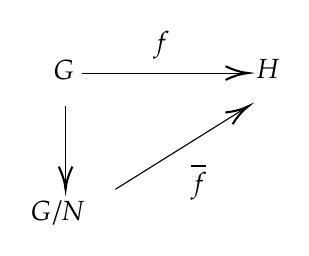
\begin{tikzpicture}[x=0.75pt,y=0.75pt,yscale=-1,xscale=1]
%uncomment if require: \path (0,476); %set diagram left start at 0, and has height of 476

%Straight Lines [id:da7538581077545223] 
\draw    (160,184) -- (238,184) ;
\draw [shift={(240,184)}, rotate = 180] [color={rgb, 255:red, 0; green, 0; blue, 0 }  ][line width=0.75]    (10.93,-3.29) .. controls (6.95,-1.4) and (3.31,-0.3) .. (0,0) .. controls (3.31,0.3) and (6.95,1.4) .. (10.93,3.29)   ;
%Straight Lines [id:da10873715429294717] 
\draw    (152,200) -- (152,238) ;
\draw [shift={(152,240)}, rotate = 270] [color={rgb, 255:red, 0; green, 0; blue, 0 }  ][line width=0.75]    (10.93,-3.29) .. controls (6.95,-1.4) and (3.31,-0.3) .. (0,0) .. controls (3.31,0.3) and (6.95,1.4) .. (10.93,3.29)   ;
%Straight Lines [id:da2888844088977629] 
\draw    (176,240) -- (238.3,201.06) ;
\draw [shift={(240,200)}, rotate = 147.99] [color={rgb, 255:red, 0; green, 0; blue, 0 }  ][line width=0.75]    (10.93,-3.29) .. controls (6.95,-1.4) and (3.31,-0.3) .. (0,0) .. controls (3.31,0.3) and (6.95,1.4) .. (10.93,3.29)   ;

% Text Node
\draw (145,176.4) node [anchor=north west][inner sep=0.75pt]    {$G$};
% Text Node
\draw (243,176.4) node [anchor=north west][inner sep=0.75pt]    {$H$};
% Text Node
\draw (134,244.4) node [anchor=north west][inner sep=0.75pt]    {$G/N$};
% Text Node
\draw (193,162.4) node [anchor=north west][inner sep=0.75pt]    {$f$};
% Text Node
\draw (211,226.4) node [anchor=north west][inner sep=0.75pt]    {$\overline{f}$};
\end{tikzpicture}
\end{center}
is commutative.
\begin{proof}
We first proof that $\overline{f}$ is well-defined. For any $b\in aN$, there exists $n\in N$ such that $b=an$. Now $f(b)=f(an)=f(a)f(n)=f(a)$ since $N\subset\mathrm{Ker}f$. Hence $\overline{f}$ has same effect on elements in $aN$. Observed that 
$$
\overline{f}\left( abN \right) =f\left( ab \right) =f\left( a \right) f\left( b \right) =\overline{f}\left( aN \right) \overline{f}\left( bN \right) ,
$$
hence $\overline{f}$ is a homomorphism. It is trivial by definition of $\overline{f}$ that $\mathrm{Im}\overline{f}=\mathrm{Im}f$. Now we proof that $\mathrm{Ker}\overline{f}=(\mathrm{Ker}f)/N$. Let $xN\in\mathrm{Ker}\overline{f}$, then $\overline{f}(xN)=f(x)=e$, hence $x\in\mathrm{Ker}f$ and therefore $xN\in(\mathrm{Ker}f/N)$. Conversely, if $yN\in(\mathrm{Ker}f)/N$, then $y\in\mathrm{Ker}f$ and hence $\overline{f}(yN)=f(y)=e$, which implies $yN\in\mathrm{Ker}\overline{f}$ and then $\mathrm{Ker}\overline{f}=(\mathrm{Ker}f)/N$. Now if $f$ is an epimorphism, then so is $\overline{f}$. If $N=\mathrm{Ker}f$, then $\mathrm{Ker}\overline{f}=\mathrm{Ker}f/\mathrm{Ker}f=\left<e\right>$. Therefore by theorem 2.9 we know that $\overline{f}$ is an isomorphism.
\end{proof}
\begin{corollary}(First Isomorphism Theorem)
If $f:G\to H$ is a homomorphism of groups, then $f$ induces an isomorphism $G/\mathrm{Ker}f\cong\mathrm{Im}f$.
\end{corollary}
This is an immediate corollary of theorem 2.35 for $G\to\mathrm{Im}f$ is epimorphic. We skip the proof.
\begin{corollary}
If $f:G\to H$ is a homomorphism of groups, $N\lhd G,M\lhd H$, and $f(N)<M$, then $f$ induces a homomorphism $\overline{f}:G/N\to H/M$, given by $aN\mapsto f(a)M$. $\overline{f}$ is an isomorphism if and only if $\mathrm{Im}f\vee M=H$ and $f^{-1}(M)\subset N$. In particular if $f$ is an epimorphism such that $f(N)=M$ and $\mathrm{Ker}f\subset N$, then $\overline{f}$ is an isomorphism.
\end{corollary}
\begin{proof}
We consider the composition 
$$
G\overset{f}{\longrightarrow}H\overset{\pi}{\longrightarrow}H/M,
$$
here $\pi f:G\to H/M$. Then by theorem 2.35 we know that $\pi f$ induces a homomorphism $\overline{f}:G/N\to H/M$ given by $aN\mapsto f(a)M$. By theorem 2.35 we know that $\overline{f}$ is an isomorphism if and only if $\pi f$ is an epimorphism and $\mathrm{Ker}\pi f=N$, which is equivalent to the condition $\mathrm{Im}f\vee M=H$ and $f^{-1}(M)\subset N$.
\end{proof}
This corollary can also be rephrased as the commutative diagram as follows:
\begin{center}
\tikzset{every picture/.style={line width=0.75pt}} %set default line width to 0.75pt        

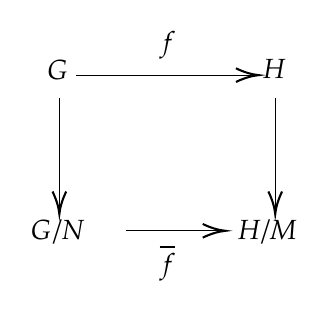
\begin{tikzpicture}[x=0.75pt,y=0.75pt,yscale=-1,xscale=1]
%uncomment if require: \path (0,476); %set diagram left start at 0, and has height of 476

%Straight Lines [id:da1481227158581686] 
\draw    (240,157) -- (326,157) ;
\draw [shift={(328,157)}, rotate = 180] [color={rgb, 255:red, 0; green, 0; blue, 0 }  ][line width=0.75]    (10.93,-3.29) .. controls (6.95,-1.4) and (3.31,-0.3) .. (0,0) .. controls (3.31,0.3) and (6.95,1.4) .. (10.93,3.29)   ;
%Straight Lines [id:da13347059157002916] 
\draw    (232,168) -- (232,222) ;
\draw [shift={(232,224)}, rotate = 270] [color={rgb, 255:red, 0; green, 0; blue, 0 }  ][line width=0.75]    (10.93,-3.29) .. controls (6.95,-1.4) and (3.31,-0.3) .. (0,0) .. controls (3.31,0.3) and (6.95,1.4) .. (10.93,3.29)   ;
%Straight Lines [id:da6724755868913452] 
\draw    (336,168) -- (336,222) ;
\draw [shift={(336,224)}, rotate = 270] [color={rgb, 255:red, 0; green, 0; blue, 0 }  ][line width=0.75]    (10.93,-3.29) .. controls (6.95,-1.4) and (3.31,-0.3) .. (0,0) .. controls (3.31,0.3) and (6.95,1.4) .. (10.93,3.29)   ;
%Straight Lines [id:da16316142037972892] 
\draw    (264,232) -- (310,232) ;
\draw [shift={(312,232)}, rotate = 180] [color={rgb, 255:red, 0; green, 0; blue, 0 }  ][line width=0.75]    (10.93,-3.29) .. controls (6.95,-1.4) and (3.31,-0.3) .. (0,0) .. controls (3.31,0.3) and (6.95,1.4) .. (10.93,3.29)   ;

% Text Node
\draw (225,148.4) node [anchor=north west][inner sep=0.75pt]    {$G$};
% Text Node
\draw (329,148.4) node [anchor=north west][inner sep=0.75pt]    {$H$};
% Text Node
\draw (217,225.4) node [anchor=north west][inner sep=0.75pt]    {$G/N$};
% Text Node
\draw (317,225.4) node [anchor=north west][inner sep=0.75pt]    {$H/M$};
% Text Node
\draw (279,134.4) node [anchor=north west][inner sep=0.75pt]    {$f$};
% Text Node
\draw (279,237.4) node [anchor=north west][inner sep=0.75pt]    {$\overline{f}$};


\end{tikzpicture}
\end{center}
\begin{corollary}(Second Isomorphism Theorem)
If $K$ and $N$ are subgroups of a group $G$, with $N$ normal in $G$, then $K/(N\cap K)\cong NK/N$.
\end{corollary}
\begin{proof}
Consider the composition 
$$
K\overset{\subset}{\longrightarrow}NK\overset{\pi}{\longrightarrow}NK/N
$$
$f$, which is a homomorphism with kernel $H\cap K$. Hence by the first Isomorphism Theorem we know that $K/(H\cap K)\cong\mathrm{Im}f$. Every element in $NK/N$ has a form of $nkN=kn^\prime N=kN$, hence $f$ is an epimorphism and $\mathrm{Im}f=KN/N$, which finished our proof.
\begin{center}
\tikzset{every picture/.style={line width=0.75pt}} %set default line width to 0.75pt        

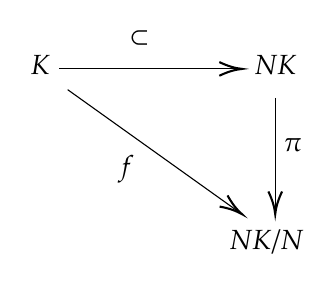
\begin{tikzpicture}[x=0.75pt,y=0.75pt,yscale=-1,xscale=1]
%uncomment if require: \path (0,476); %set diagram left start at 0, and has height of 476

%Straight Lines [id:da6768105974377752] 
\draw    (264,146) -- (350,146) ;
\draw [shift={(352,146)}, rotate = 180] [color={rgb, 255:red, 0; green, 0; blue, 0 }  ][line width=0.75]    (10.93,-3.29) .. controls (6.95,-1.4) and (3.31,-0.3) .. (0,0) .. controls (3.31,0.3) and (6.95,1.4) .. (10.93,3.29)   ;
%Straight Lines [id:da9794328893642172] 
\draw    (368,160) -- (368,214) ;
\draw [shift={(368,216)}, rotate = 270] [color={rgb, 255:red, 0; green, 0; blue, 0 }  ][line width=0.75]    (10.93,-3.29) .. controls (6.95,-1.4) and (3.31,-0.3) .. (0,0) .. controls (3.31,0.3) and (6.95,1.4) .. (10.93,3.29)   ;
%Straight Lines [id:da5963291247279754] 
\draw    (268,156) -- (350.37,214.84) ;
\draw [shift={(352,216)}, rotate = 215.54] [color={rgb, 255:red, 0; green, 0; blue, 0 }  ][line width=0.75]    (10.93,-3.29) .. controls (6.95,-1.4) and (3.31,-0.3) .. (0,0) .. controls (3.31,0.3) and (6.95,1.4) .. (10.93,3.29)   ;

% Text Node
\draw (249,138.4) node [anchor=north west][inner sep=0.75pt]    {$K$};
% Text Node
\draw (357,138.4) node [anchor=north west][inner sep=0.75pt]    {$NK$};
% Text Node
\draw (345,222.4) node [anchor=north west][inner sep=0.75pt]    {$NK/N$};
% Text Node
\draw (297,126.4) node [anchor=north west][inner sep=0.75pt]    {$\subset $};
% Text Node
\draw (371,178.4) node [anchor=north west][inner sep=0.75pt]    {$\pi $};
% Text Node
\draw (291,186.4) node [anchor=north west][inner sep=0.75pt]    {$f$};
\end{tikzpicture}
\end{center}
\end{proof}
\begin{corollary}(Third Isomorphism Theorem)
If $H$ and $K$ are normal subgroups of a group $G$ such that $K<H$, then $H/K$ is a normal subgroup of $G/K$ and $(G/K)(H/K)\cong G/H$.
\end{corollary}
\begin{proof}
Define $f:G/K\rightarrow G/H$ by $aK\mapsto aH$. From $K<H$ we know that $f$ is an epimorphism. Consider the kernel of $f$, we have 
$$
\mathrm{Ker}f=\left\{ aK:a\in H \right\} =H/K
$$
since $f(aK)\in H$ if and only if $a\in H$. Therefore $\mathrm{Ker}f=H/K\lhd G/K$ and hence 
$$
\mathrm{Im}f=G/H\cong \left( G/K \right) /\left( \mathrm{Ker}f \right) =\left( G/K \right) /\left( H/K \right) .
$$
\begin{center}
\tikzset{every picture/.style={line width=0.75pt}} %set default line width to 0.75pt        

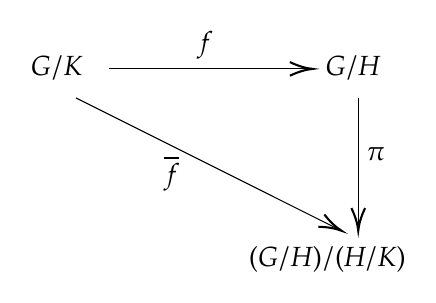
\begin{tikzpicture}[x=0.75pt,y=0.75pt,yscale=-1,xscale=1]
%uncomment if require: \path (0,476); %set diagram left start at 0, and has height of 476

%Straight Lines [id:da6750362936107648] 
\draw    (248,162) -- (344,162) ;
\draw [shift={(346,162)}, rotate = 180] [color={rgb, 255:red, 0; green, 0; blue, 0 }  ][line width=0.75]    (10.93,-3.29) .. controls (6.95,-1.4) and (3.31,-0.3) .. (0,0) .. controls (3.31,0.3) and (6.95,1.4) .. (10.93,3.29)   ;
%Straight Lines [id:da9589750420240954] 
\draw    (368,176) -- (368,238) ;
\draw [shift={(368,240)}, rotate = 270] [color={rgb, 255:red, 0; green, 0; blue, 0 }  ][line width=0.75]    (10.93,-3.29) .. controls (6.95,-1.4) and (3.31,-0.3) .. (0,0) .. controls (3.31,0.3) and (6.95,1.4) .. (10.93,3.29)   ;
%Straight Lines [id:da8916432325404353] 
\draw    (232,176) -- (358.21,239.11) ;
\draw [shift={(360,240)}, rotate = 206.57] [color={rgb, 255:red, 0; green, 0; blue, 0 }  ][line width=0.75]    (10.93,-3.29) .. controls (6.95,-1.4) and (3.31,-0.3) .. (0,0) .. controls (3.31,0.3) and (6.95,1.4) .. (10.93,3.29)   ;

% Text Node
\draw (209,154.4) node [anchor=north west][inner sep=0.75pt]    {$G/K$};
% Text Node
\draw (351,154.4) node [anchor=north west][inner sep=0.75pt]    {$G/H$};
% Text Node
\draw (314,246.4) node [anchor=north west][inner sep=0.75pt]    {$( G/H) /( H/K)$};
% Text Node
\draw (289,142.4) node [anchor=north west][inner sep=0.75pt]    {$f$};
% Text Node
\draw (371,198.4) node [anchor=north west][inner sep=0.75pt]    {$\pi $};
% Text Node
\draw (273,202.4) node [anchor=north west][inner sep=0.75pt]    {$\overline{f}$};


\end{tikzpicture}
\end{center}
\end{proof}
\begin{theorem}
If $f:G\to H$ is an isomorphism of groups, then the assignment $K\mapsto f(K)$ defines a one-to-one correspondence between the set $S_f(G)$ of all subgroups $K$ of $G$ which contain $\mathrm{Ker}f$ and the set $S(H)$ of all subgroups of $H$. Under this correspondence normal subgroups correspond to normal subgroups.
\end{theorem}
\begin{proof}
Denote $\varphi:S_f(G)\to S(H)$ given by $K\mapsto f(K)$. We first proof that $\varphi$ is bijective. By exercise 2.20 we know that for all $J\in S(H)$, $f^{-1}(J)$ is a subgroup of $G$. Since $J<H$, we have $\mathrm{Ker}f<f^{-1}(J)$ and hence $f(f^{-1}(J))=J$. That is, for all $J\in S(H)$, there exists $f^{-1}(J)\in S_f(G)$ such that $f(f^{-1}(J))=J$, hence $\varphi$ is surjective. By an exercise of this section(we shall admit this to be true here) we know that $f^{-1}(f(J))=J$ if and only if $\mathrm{Ker}f<J$, which is
$$
f\left( K \right) =f\left( J \right) \Rightarrow K=f^{-1}\left( f\left( K \right) \right) =f^{-1}\left( f\left( J \right) \right) =J\Rightarrow K=J,
$$
hence $\varphi$ is injective. For the last statement, we proof that $K\lhd G$ implies $f(K)\lhd H$, which is easy to verify by definition of a normal group. Similarly we have $J\lhd H$ implies $f^{-1}(J)\lhd G$.
\end{proof}
\begin{corollary}
If $G$ is a group and $N$ is a normal subgroup of $G$, then every subgroup of $G/N$ has a form of $K/N$, where $K$ is a subgroup of $G$ that contains $N$. Furthermore, $K/N$ is normal in $G/N$ if and only if $K$ is normal in $G$.
\end{corollary}
\begin{proof}
Apply theorem 2.40 to the canonical mapping $\pi:G\to G/N$. It is familiar to us that $\mathrm{Ker}\pi=N$, hence by theorem 2.40, any subgroup $K$ satisfies $N<K<G$ corresponds with a subgroup $K/N$ satisfies $K/N<G/N$. Since the correspondence is one-to-one, we know all subgroups of $G/N$ has such a form.Also if $K/N$ is a normal subgroup of $G/N$, then $K\lhd G$.The converse statement is also true since the correspondence is one-to-one.
\end{proof}
\begin{center}
\begin{large}
    \textbf{Exercises for 2.5}
\end{large}
\end{center}
\begin{problem}\em
If $N$ is a subgroup of index $2$ in a group $G$, then $N$ is normal in $G$.
\end{problem}
\begin{proof}
We consider all cosets of $N$ in $G$. Clearly $N$ itself is a coset of $N$. Since $[G:N]=2$, then another coset is the complement of $N$ since cosets completely separated $G$. Observed the discussion above does not involve the concept of a left coset or right coset, hence they are totally symmetric. By definition of normal group we have $N\lhd G$.
\end{proof}
\begin{problem}\em
If $\{N_i:i\in I\}$ is a family of normal subgroups of $G$, then $\bigcap_{i\in I}N_i$ is a normal subgroup of $G$.
\end{problem}
\begin{proof}
We proof by definition. Take $n\in\bigcap_{i\in I}N_i$, then for any $i\in I$ and $a\in G$ we have $ana^{-1}\in N_i$ since $N_i\lhd G$. Since this is generally true for all $i\in I$, we know that $ana^{-1}\in\bigcap_{i\in I}N_i$, which implies $a\left(\bigcap_{i\in I}N_i\right)a^{-1}\subset\bigcap_{i\in I}N_i$ and hence $\left(\bigcap_{i\in I}N_i\right)\lhd G$.
\end{proof}
\begin{problem}\em
Let $N$ be a subgroup of $G$. $N$ is normal in $G$ if and only if (right) congruence modulo $N$ is a congruence relation on $G$.
\end{problem}
\begin{proof}
Suppose $N$ is normal in $G$. If $a_1\equiv b_1(\mathrm{mod}N)$ and $a_2\equiv b_2(\mathrm{mod}N)$, then $a_1b_1^{-1}\in N,a_2b_2^{-1}\in N$. It suffices to show that $a_1a_2b_2^{-1}b_1^{-1}\in G$, which can be obtained by the same trick used in Theorem 2.33. Conversely, by definition of a congruence relation and $n\equiv e(\mathrm{mod}N)$, $a\equiv a(\mathrm{mod}N)$, here $n\in N$ and $a\in G$ are arbitrarily chosen, we have $an\equiv a(\mathrm{mod}N)$ and hence $ana^{-1}\in N$. Therefore $aNa^{-1}\subset N$ for all $a\in G$ and hence $N\lhd G$.
\end{proof}
\begin{problem}\em
Let $\sim$ be an equivalence relation on a group $G$ and let $N=\{a\in G:a\sim e\}$. Then $\sim$ is a congruence relation on $G$ if and only if $N$ is a normal subgroup of $G$ and $\sim$ is congruence modulo $N$.
\end{problem}
\begin{proof}
Let $\sim$ be a congruence relation on $G$. Hence for all $n\in N$ and $a\in G$ we have $ana^{-1}\sim e$ by the same method used in exercise 2.56, hence $ana^{-1}\in N$. Therefore $aNa^{-1}\in N$ and $N\lhd G$. What's more, if $a\sim b$, then $ab^{-1}\sim e$, which is $ab^{-1}\in N$, hence $\sim$ is congruence modulo $N$. The converse condition is trivial.
\end{proof}
\begin{problem}\em
Let $N<S_4$ consist of all those permutations $\sigma$ such that $\sigma(4)=4$. Is $N$ normal in $S_4$?
\end{problem}
\begin{proof}
No. Take 
$$
\sigma =\left( \begin{matrix}
	1&		2&		3&		4\\
	2&		3&		1&		4\\
\end{matrix} \right) \in N,\tau =\left( \begin{matrix}
	1&		2&		3&		4\\
	2&		3&		4&		1\\
\end{matrix} \right) \in S_4,
$$
then $\tau \sigma \tau ^{-1}\left( 4 \right) =2\ne 4$, hence $\tau\sigma\tau^{-1}\notin N$.
\end{proof}
\begin{problem}\em
Let $H<G$. Then the set $aHa^{-1}$ is a subgroup for each $a\in G$, and $H\cong aHa^{-1}$.
\end{problem}
\begin{proof}
First since $H$ is a subgroup then $e\in H$, we know that $e=aa^{-1}=aea^{-1}\in aHa^{-1}$. Then if $aha^{-1}\in aHa^{-1}$, since $G$ and $H$ are all groups, we have $a^{-1}\in G$ and $h^{-1}\in H$, therefore $ah^{-1}a^{-1}\in aHa^{-1}$. Hence $aHa^{-1}$ is a subgroup of $G$. Now define $f:aHa^{-1}\to H$ by $aha^{-1}\mapsto h$, it is easy to verify $f$ is an isomorphism and hence $H\cong aHa^{-1}$.
\end{proof}
\begin{problem}\em
Let $G$ be a finite group and $H$ be a subgroup of $G$ ordered $n$. If $H$ is the only subgroup of $G$ of order $n$, then $H$ is normal in $G$.
\end{problem}
\begin{proof}
Let $a\in G$. Then by exercise 2.59 we know that $H\cong aHa^{-1}$. Therefore $aHa^{-1}$ is also a subgroup of $G$ with order $n$. However there is only one such subgroup, we have $H=aHa^{-1}$ and hence $H\lhd G$.
\end{proof}
\begin{problem}\em
All subgroups of the quaternion group are normal.
\end{problem}
\begin{proof}
We denote 
$$
I=\left( \begin{matrix}
	0&		\mathrm{i}\\
	\mathrm{i}&		0\\
\end{matrix} \right) ,J=\left( \begin{matrix}
	0&		1\\
	1&		0\\
\end{matrix} \right) ,K=\left( \begin{matrix}
	\mathrm{i}&		0\\
	0&		-\mathrm{i}\\
\end{matrix} \right) ,L=-I.
$$
Then subgroups of $Q_8$ are $0,\left< L \right> ,\left< I \right> ,\left< J \right> ,\left< K \right> ,Q_8$. Both $0$ and $Q_8$ are trivial normal subgroups. Subgroups generated by $I,J$ and $K$ have an order $2$. Finally $L$ is the intersection of normal groups. Hence by exercise 2.54 and exercise 2.55 we finished our proof.
\end{proof}
\begin{note}\em
Notice that $Q_8$ is non-abelian. This exercise gives an example that a group with all its subgroups normal may not be abelian.
\end{note}
\begin{problem}\em
(a) If $G$ is a group, then the center of $G$ is normal subgroup of $G$.\par
(b) The center of $S_n$ is the identity subgroup for all $n>2$.
\end{problem}
\begin{proof}
(a) We denote the center of $G$ as $C$. For all $x\in C$ we have $ax=xa$, where $a\in G$ is arbitrarily chosen. Hence $aC=Ca$ holds for all $a$ and therefore $C\lhd G$.\par
(b) We denote the center of $S_n$ as $Z(S_n)$. If there exists such an element $\sigma$ that $\sigma\ne(1)$, WLOG we suppose $\sigma(1)=2$, then for $\tau=(23)$, we observed that $\sigma\tau(1)=2$ and $\tau\sigma=3$, which contradicts to the definition of the center of a group.
\end{proof}
\begin{problem}\em
Find subgroups $H$ and $K$ of $D_4^*$ such that $H\lhd K$ and $K\lhd D_4^*$, but $H$ is not normal in $D_4^*$.
\end{problem}
\begin{proof}
Consider the subgroup $H$ generated by $T_x$, which is a subgroup of the group $K$ generated by $R^2$ and $T_x$ with index $2$. Therefore by exercise 2.54 we know that $H$ is normal in $K$. Also $K$ is a subgroup of index $2$ in $D_4^*$, hence $K$ is normal in $D_4^*$. However, we may check that $H$ is not normal in $D_4^*$.
\end{proof}
\begin{note}\em
This exercise provided an example that normality may not be transitive.
\end{note}
\begin{problem}\em
If $H$ is a cyclic subgroup of a group $G$ and $H$ is normal in $G$, then every subgroup of $H$ is normal in $G$.
\end{problem}
\begin{proof}
Let $H=\left<a\right>$. Then if $K$ is a subgroup of $H$, take $k\in K$, it has the form $k=a^j$, here $j\in\mathbb{Z}$. Since $H$ is normal in $G$, then for all $g\in G$ we have $ga^jg^{-1}=(gag^{-1})^k=a^{mk}\in K$, hence $gKg^{-1}\subset K$ and therefore $K$ is normal in $G$.
\end{proof}
\begin{problem}\em
If $H$ is a normal subgroup of a group $G$ such that $H$ and $G/H$ are finitely generated, then so is $G$.
\end{problem}
\begin{proof}
Suppose $H$ is generated by a finite set $X$ and $G/H$ is generated by a finite group $Y$. It suffices to show that $G$ is generated by $X\cup Y$. Now observed that 
$$
G=\bigcup_{a\in G}{aH}=\bigcup_{x_i\in X}{\left( \prod_i{x_{i}^{r_i}H} \right)}=\bigcup_{x_i\in X}{\left( \prod_i{x_{i}^{r_i}\left( \bigcup_{y_j\in Y}{\prod_j{y_{j}^{s_j}}} \right)} \right)}=\bigcup_X{\bigcup_Y{\left( \prod_i{\prod_j{x_{i}^{r_i}y_{j}^{s_j}}} \right)}},
$$
hence $G$ is generated by $X\cup Y$ and we finished our proof.
\end{proof}
\begin{problem}\em
Let $H\lhd G,K\lhd G$. Show that $H\vee K$ is normal in $G$.
\end{problem}
\begin{proof}
Since $H$ and $K$ are normal in $G$, then $H\vee K=HK$ by Theorem 2.32. Hence for all $x\in H\vee K$, we may set $x=hk$. Now since $H$ and $K$ are all normal in $G$, for all $g\in G$ we have $gxg^{-1}=ghgg^{-1}kg\in HK$, hence $gHKg^{-1}\subset HK$ and therefore $H\vee K=HK$ is normal in $G$.
\end{proof}
\begin{problem}\em
If $N_1\lhd G_1,N_2\lhd G_2$ then $(N_1\times N_2)\lhd(G_1\times G_2)$ and $(G_1\times G_2)/(N_1\times N_2)\cong(G_1/N_1)\times(G_2/N_2)$.
\end{problem}
\begin{proof}
Let $(n_1,n_2)\in N_1\times N_2$. Then for $(g_1,g_2)\in G_1\times G_2$, then since $N_1\lhd G_1,N_2\lhd G_2$ we know that 
$$
\left( g_1,g_2 \right) \left( n_1,n_2 \right) \left( g_1,g_2 \right) ^{-1}=\left( g_1n_1g_{1}^{-1},g_2n_2g_{2}^{-1} \right) \in N_1\times N_2,
$$
hence $\left( g_1,g_2 \right) \left( N_1\times N_2 \right) \left( g_1,g_2 \right) ^{-1}\subset N_1\times N_2$, whence $N_1\times N_2$ is normal in $G_1\times G_2$. Now define $f:(G_1\times G_2)/(N_1\times N_2)\to(G_1/N_1)\times(G_2/N_2)$ by $\left( g_1,g_2 \right) \left( N_1\times N_2 \right) \mapsto \left( g_1N_1,g_2N_2 \right) $, it is easy to verify that $f$ is an isomorphism.
\end{proof}
\begin{problem}\em
Let $N\lhd G$ and $K\lhd G$. If $N\cap K=\left<e\right>$ and $N\vee K=G$, then $G/N\cong K$.
\end{problem}
\begin{proof}
We proof by the Second Homomorphism Theorem, by which we know that $HN/N\cong K/(H\cap K)$. However, since $N$ and $K$ are normal in $G$, we know by theorem 2.32 that $HN=H\vee N=G$. Also observed that $N\cap K=\left<e\right>$, hence $HN/N=G/N\cong K/(N\cap K)=K$.
\end{proof}
\begin{problem}\em
If $f:G\to H$ is a homomorphism, $H$ is abelian and $N$ is a subgroup of $G$ containing $\mathrm{Ker}f$, then $N$ is normal in $G$.
\end{problem}
\begin{proof}
We proof by the First Homomorphism Theorem, by which we know that $G/\mathrm{Ker}f\cong\mathrm{Im}f$. It suffices to show that $N/\mathrm{Ker}f\lhd G/\mathrm{Ker}f$ by theorem 2.40. Since $G/\mathrm{Ker}f\cong\mathrm{Im}f$, we only need to proof $N/\mathrm{Ker}f\lhd\mathrm{Im}f$. Since $H$ is abelian and $\mathrm{Im}f$ is a subgroup of $H$, clearly $\mathrm{Im}f$ is also abelian. Then $N/\mathrm{Ker}f\lhd\mathrm{Im}f$ follows immediately since all subgroups of an abelian group are normal, since $aha^{-1}=aa^{-1}h=h\in H$ for all $h\in N/\mathrm{Ker}f$ and $a\in\mathrm{Im}f$.
\end{proof}
\begin{problem}\em
(a) Consider the subgroups $\left<6\right>$ and $\left<30\right>$ of $\mathbb{Z}$ and show that $\left<6\right>/\left<30\right>\cong\mathbb{Z}_5$.\par
(b) For any $k,m>0$, $\left<k\right>/\left<km\right>\cong\mathbb{Z}_m$. In particular, $\mathbb{Z}/\left<m\right>\cong\mathbb{Z}_m$.
\end{problem}
\begin{proof}
(a) Observed that 
$$\left<6\right>/\left<30\right>=\{\left<30\right>,6+\left<30\right>,12+\left<30\right>,18+\left<30\right>,24+\left<30\right>\},$$
we may define $f:\left<6\right>/\left<30\right>\to\mathbb{Z}_5$ by $6m+\left<30\right>\mapsto\overline{m}$, which is easy to verify to be an isomorphism.\par
(b) Observed that 
$$
\left< m \right> /\left< km \right> =\left\{ \left< km \right> ,m+\left< km \right> ,2m+\left< km \right> ,\cdots ,\left( k-1 \right) m+\left< km \right> \right\} ,
$$
by same method used for (a) we may define an isomorphism from $\left<m\right>/\left<km\right>$ to $\mathbb{Z}_m$, which shows that $\left<k\right>/\left<km\right>\cong\mathbb{Z}_m$.
\end{proof}
\begin{problem}\em
If $f:G\to H$ is a homomorphism with kernel $N$ and $K<G$, then prove that $f^{-1}(f(K))=KN$.
\end{problem}
\begin{proof}
First observed 
$$
\begin{aligned}
f^{-1}\left( f\left( K \right) \right) &=\left\{ x\in G:f\left( k \right) =f\left( x \right) \,\,\mathrm{for} \mathrm{some} k\in K \right\} 
\\
&=\left\{ x\in G:kx^{-1}\in N,\in K \right\} =\left\{ x\in G:x\in kN,k\in K \right\} \subset KN,
\end{aligned}
$$
hence $f^{-1}f(K)\subset KN$. Conversely, for $x\in KN$, let $x=kn$, then 
$$
f^{-1}\left( f\left( kn \right) \right) =f^{-1}\left( f\left( k \right) f\left( n \right) \right) =f^{-1}\left( f\left( k \right) \right) \in f^{-1}\left( f\left( K \right) \right) ,
$$
therefore $f^{-1}(f(K))\supset KN$, hence $f^{-1}(f(K))=KN$.
\end{proof}
\begin{note}\em
By this exercise we know that $f^{-1}(f(K))=K$ if and only if $N<K$, which is used in the proof of theorem 2.40.
\end{note}
\begin{problem}\em
If $N\lhd G$, $[G:N]$ finite, $H<G$, $G$ finite, and $[G:N]$ and $|H|$ are relatively prime, then $H<N$.
\end{problem}
\begin{proof}
Let $G=N\cup a_1N\cup \cdots \cup a_nN$. It suffices to show $N\subset H$. Let $a\in H$, then $a=a_in,n\in N,i\in\{1,2,\cdots,n\}$. Since $N$ is normal in $G$, we have $(a_in)^{|H|}=e\Rightarrow a_i^{|H|}n^{|H|}=e$. However $a_i^{[G:N]}=e$ and $[G:N]$ and $|H|$ are relatively prime, hence $a_i\in N$, which implies $a\in N$ and we finished our proof.
\end{proof}
\begin{problem}\em
Let $H\ne\mathbb{Z}(p^\infty)$ be a subgroup of $\mathbb{Z}(p^\infty)$, prove that $\mathbb{Z}(p^\infty)/H\cong\mathbb{Z}(p^{\infty})$.
\end{problem}
\begin{proof}
First $H$ must be a cyclic subgroup with all its elements have a finite order by exercise 2.36. Let $H_i=\left<\overline{1/p^i}\right>$. Now we have the canonical projection homomorphisms $\pi_i:\mathbb{Z}(p^\infty)\to\mathbb{Z}(p^\infty)/H_i$. Notice the image contains elements $x_n=\overline{1/p^{n+i}}+H_i$, therefore
$$
px_{n+1}=pf\left( \overline{1/p^{\left( n+1 \right) +i}} \right) =f\left( \overline{p/p^{\left( n+1 \right) +i}} \right) =f\left( \overline{1/p^{n+i}} \right) =x_n,
$$
Also $i$ is finite, so $x_n$ exists for any $n\in\mathbb{Z}_+$. Therefore by exercise 2.36 we know that $\mathbb{Z}(p^\infty)/H\cong\mathbb{Z}(p^{\infty})$.
\end{proof}
\subsection{Symmetric, Alternating, and Dihedral Groups}
In this section we shall study in some detail the symmetric group $S_n$ and its subgroups. By definition $S_n$ is a bijection $I_n\to I_n$, where $I_n=\{1,2,\cdots,n\}$. We first introduce another notation of a permutation:
\begin{definition}
Let $i_1,i_2,\cdots,i_r$ be distinct elements of $I_n$, here $r\le n$. Then $(i_1i_2\cdots i_n)$ denotes a permutation that maps $i_1\mapsto i_2,i_2\mapsto i_3,\cdots,i_r\mapsto i_1$, and maps every other elements in $I_n$ onto itself. $(i_1i_2\cdots i_n)$ is called a \textbf{cycle with length $r$} or an \textbf{$r$-cycle}. In particular, a $2$-cycle is called a \textbf{transposition}.
\end{definition}
Here are some examples.
\begin{example}\em
A permutation $
\sigma =\left( \begin{matrix}
	1&		2&		3&		4\\
	2&		3&		4&		1\\
\end{matrix} \right) 
$ is a $4$-cycle denote as $(1234)$ or $(2341)$ or $(3412)$ or $(4123)$.
\end{example}
As we can see a cycle may be written in many different ways. However, one may eliminate ambiguities by context.\par
There is one condition that some cycles are commute.
\begin{definition}
The permutations $\sigma_1,\sigma_2,\cdots,\sigma_r$ of $S_n$ is said to be \textbf{disjoint} provided for each $1\le i\le r$, and every $k\in I_n,\sigma_i(k)\ne k$ implies $\sigma_j(k)=k$ for all $j\ne i$.
\end{definition}
In other words, $\sigma_1,\sigma_2,\cdots,\sigma_r$ are said to be disjoint if and only if no element of $I_n$ is moved by more than one of $\sigma_i,1\le i\le r$.
\begin{example}\em
In $S_4$, the transposition $(13)$ and $(24)$ are disjoint. It is easy to verify that disjoint cycles are commute since every element is only moved once.
\end{example}
We have the important theorem as follows:
\begin{theorem}
Every non-identity permutation in $S_n$ is uniquely a product of disjoint cycles, each of which has length at least $2$.
\end{theorem}
\begin{proof}
Let $\sigma$ be a non-trivial permutation in $S_n$. We first proof that there exists some disjoint cycles of length at least $2$, such that $\sigma$ is the product of them. We begin by define a relation on $I_n$: $a\sim b$ for $a,b\in I_n$ if and only if $b=\sigma^m(a)$ for some $m\in\mathbb{Z}$. Now we proof $\sim$ is an equivalence relation:\par
(i) $a\sim a$: This is trivial.\par
(ii) $a\sim b\Rightarrow b\sim a$: By $a\sim b$ we know that there exists $m\in\mathbb{Z}$ such that $b=\sigma^m(a)$, hence $a=\sigma^{-m}(b)$ and therefore $a\sim b$.\par
(iii) $a\sim b,b\sim c\Rightarrow a\sim c$: By $a\sim b$ and $b\sim c$ we know that there exists $m,n\in\mathbb{Z}$ such that $b=\sigma^m(a)$ and $c=\sigma^n(b)$, hence $c=\sigma^{m+n}(a)$, therefore $a\sim c$.\par
Now $\sim$ is an equivalence relation and therefore it induces equivalence classes $\{B_i\}$, where $B_i=\{x:x\sim x_i\}=\{\sigma^m(x_i):m\in\mathbb{Z}\}$, here $x_i$ is a select element in $I_n$. By properties of equivalent classes we know $B_i$ are disjoint. We call $B_i=\{\sigma^m(x_i):m\in\mathbb{Z}\}$ the \textbf{orbit of $x_i$ generated by $\sigma$}. Now we define $
\sigma _i\left( x \right) =\begin{cases}
	\sigma \left( x \right) ,x\in B_i,\\
	x,x\notin B_i,\\
\end{cases}
$ it is easy to verify $\sigma=\sigma_1\sigma_2\cdots\sigma_s$, here we assume the index class of $\{B_i\}$ is $1,2,\cdots,s$, that is, $1\le i\le s$. Now it suffices to show that for any $x\in I_n$ there exists $d\in\mathbb{Z}_+$ such that $\sigma^d(x)=x$, since $\sigma_j$ are disjoint and hence $\sigma(x)=\sigma_i(x)$ for some $i\in I_s$. First, we know that there exists a least $d$ such that $\sigma^d(x)=\sigma^j(x)$ for some $0\le j<d$, since $S_n$ is obviously finite. Therefore $\sigma^{d-j}(x)=x$, which forces $j=0$ and $\sigma^d(x)=x$. Now for any $m\in\mathbb{Z}$, there exists $a,b\in\mathbb{Z}$ such that $m=ad+b$, hence $\sigma^m(x)=\sigma^{ad+b}(x)=\sigma^b(x)\in B_i$ for a unique $i\in I_s$, therefore we proved that $\sigma_i$ is a cycle. Since $x\in I_n$ is arbitrarily chosen, the result is true for all $\sigma_j$.\par
Now we proof that the product of disjoint cycles are unique. If there is another presentation $\tau_1\tau_2\cdots\tau_t$, then for all $x\in I_n$, there exists unique $i$ and $j$ such that $\sigma_i(x)=\tau_j(x)$. Since $\sigma\tau_j=\tau_j\sigma$, we know that the orbit generated by $\sigma_i$ is precisely the orbit generated by $\tau_j$, and since permutations discussed here are all cycles, it suffices to show that cycles have only one non-trivial orbit. Let $(i_1i_2\cdots i_r)$ be a cycle. If $i_k\ne i_j,j=1,2,\cdots,r$, then $i_k$ generates a trivial orbit. Otherwise we have the orbit 
$$
i_k\rightarrow i_{k+1}\rightarrow \cdots \rightarrow i_r\rightarrow i_1\rightarrow \cdots \rightarrow i_{k-1},
$$
which is easy to see is equivalent for all $k\in I_r$. Hence by induction we finished our proof.
\end{proof}
\begin{corollary}
The order of a permutation $\sigma\in S_n$ is the least common multiple of the orders of its disjoint cycles.
\end{corollary}
\begin{proof}
By theorem 2.44 we know that $\sigma$ can be written as the product of some cycles $\sigma_1\sigma_2\cdots\sigma_r$. Now if $\sigma^m(x)=x$ for all $x\in I_n$, then $\sigma_j^m(x)=x$ for all $j=1,2,\cdots,r$. Therefore $m$ is multiple of the order of $\sigma_j$. Since this is true for all $j=1,2,\cdots,r$, we finished our proof.
\end{proof}
\begin{corollary}
Every permutation in $S_n$ can be written as a product of some transpositions(not necessarily disjoint).
\end{corollary}
\begin{proof}
By theorem 2.44 we know that $\sigma\in S_n$ can be written as the product of some cycles $\sigma_1\sigma_2\cdots\sigma_r$. It suffices to show that for all cycles $\sigma_j$, it can be written as product of some transpositions. This is clearly true since if the length of cycle is $2$, then it itself is a transposition, otherwise let $(i_1i_2\cdots i_r)$ be the cycle, observed that $(i_1i_2\cdots i_r)=(i_1i_r)(i_2i_r)\cdots(i_{r-1}i_r)$.
\end{proof}
\begin{definition}
A permutation $\tau\in S_n$ is said to be \textbf{even} [resp. \textbf{odd}] if $\tau$ can be written as a product of an even [resp. odd] number of transpositions.
\end{definition}
We have to check if an even [resp. odd] permutation is well-defined. That is, can a permutation be both even and odd?
\begin{theorem}
A permutation in $S_n(n\ge 2)$ is either odd or even.
\end{theorem}
\begin{proof}
Let $i_1,i_2,\cdots,i_n$ be integers $1,2,\cdots,n$ in some order. Define 
$$
\Delta \left( i_1,i_2,\cdots ,i_n \right) =\prod_{1\le j<k\le n}{\left( i_j-i_k \right)}.
$$
It is clear that $\Delta(i_1,i_2,\cdots,i_n)\ne 0$. Let $\sigma=(i_ci_d)$ be a transposition and we compute $\Delta(\sigma(i_1),\sigma(i_2),\cdots,\sigma(i_n))$:
$$
\Delta \left( \sigma \left( i_1 \right) ,\sigma \left( i_2 \right) ,\cdots ,\sigma \left( i_n \right) \right) =\prod_{1\le j<k\le n}{\left( \sigma \left( i_j \right) -\sigma \left( i_k \right) \right)}=\prod_{j<k,j,k\ne c,d}{\left( i_j-i_k \right)}\cdot \left( i_d-i_c \right) .
$$
Hence $\Delta(i_1,i_2,\cdots,i_n)=-\Delta(\sigma(i_1),\sigma(i_2),\cdots,\sigma(i_n))$. Now suppose $\sigma\in S_n$ is both even and odd, then 
$$
\Delta \left( \sigma \left( i_1 \right) ,\sigma \left( i_2 \right) ,\cdots ,\sigma \left( i_n \right) \right) =\left( -1 \right) ^s\Delta \left( i_1,i_2,\cdots ,i_n \right) =\left( -1 \right) ^t\Delta \left( i_1,i_2,\cdots ,i_n \right) ,
$$
therefore $\Delta(i_1,i_2,\cdots,i_n)=0$, a contradiction!
\end{proof}
\begin{theorem}
For each $n\ge 2$, let $A_n$ be the set of all even permutations of $S_n$. Then $A_n$ is a normal subgroup of $S_n$ of index $2$ and order $\frac{|S_n|}{2}$. Furthermore, $A_n$ is the only subgroup of $S_n$ of index $2$.
\end{theorem}
\begin{proof}
Let $C$ be the multiplicative group $\{-1,1\}$. Define a homomorphism $f:S_n\to C$ by $\sigma\mapsto\mathrm{sgn}\sigma$, where $\mathrm{sgn}\sigma$ is defined as follows:
$$
\mathrm{sgn} \sigma =\begin{cases}
	1,\sigma \,\,\mathrm{is}\, \mathrm{even},\\
	-1,\sigma \,\,\mathrm{is}\, \mathrm{odd},\\
\end{cases}
$$
Then by the First Isomorphism Theorem we have $S_n/\mathrm{Ker}f\cong\mathrm{Im}f$, where $\mathrm{Ker}f=A_n$. Since $\mathrm{Ker}f\lhd S_n$ we know that $A_n\lhd S_n$. What's more, $\mathrm{Im}f=C$ and hence $S_n/A_n\cong C$, therefore $[S_n:A_n]=2$ and $|A_n|=\frac{|S_n|}{2}$. We will proof the uniqueness in exercises.
\end{proof}
\begin{note}\em
The group $A_n$ is called the \textbf{alternating group on $n$ letters} or the \textbf{alternating group of degree $n$}.
\end{note}
\begin{definition}
A group $G$ is said to be \textbf{simple} if $G$ has no proper normal subgroups.
\end{definition}
The only abelian simple groups are $\mathbb{Z}_p$ where $p$ is prime as shown in exercise 2.42. There are many non-abelian simple groups. Now we proof that all $A_n$ except $A_4$ are simple groups.
\begin{theorem}
The alternating group $A_n$ is simple if and only if $n\ne 4$.
\end{theorem}
\begin{proof}
Let $N$ be a nontrivial normal subgroup of $A_n$. We proof $N=A_n$ by several steps.\par
(i) $N$ contains a $3$-cycle. Let $\sigma\in N$. First of all $\sigma$ must rearrange the position of at least $3$ elements in $I_n$, or otherwise $\sigma$ is a transposition, which is odd. If $\sigma$ rearrange precisely $4$ elements in $I_n$, then $\sigma=(a_1a_2)(a_3a_4)$, where $a_i(1\le i\le 4)$ are elements of $I_n$ being rearranged. Since $n\ge 5$, $\beta(a_3a_4a_5)\in A_n$, hence $\sigma_1=\beta\sigma\beta^{-1}=(a_1a_3a_4a_2\cdots)\cdots\in N$. Therefore $\sigma\sigma_1=(a_3a_4)(a_4a_5)=(a_3a_4a_5)\in N$. If $\sigma$ rearrange at least $5$ elements, then we discuss each case below separately:\par
\textbf{Case 1}: $\sigma$ contains a cycle of length more than $4$. Let $\sigma=(a_1a_2a_3a_4\cdots)\cdots$. Take $\beta=(a_2a_3a_4)\in A_n$, therefore $\sigma_1=\beta\sigma\beta^{-1}=(a_1a_3a_4a_2\cdots)\cdots\in N$. Hence there are at most $4$ elements being rearranged in $\sigma_1\sigma^{-1}$, a contradiction!\par
\textbf{Case 2}: $\sigma$ has its longest cycle of length $3$. Let $\sigma=(a_1a_2a_3)(a_4a_5\cdots)\cdots$. Since $\sigma$ rearranges at least $5$ elements in $I_n$, $\sigma$ is not a cycle of length $3$. Hence such $\sigma$ must rearrange at least $6$ elements. Take $\beta=(a_2a_3a_4)\in A_n$, then $\sigma_1=\beta\sigma\beta^{-1}=(a_1a_3a_4)(a_2a_5\cdots)\cdots\in N$, which rearrange at most $5$ elements, a contradiction!\par
\textbf{Case 3}: $\sigma$ be the product of some transpositions. Let $\sigma=(a_1a_2)(a_3a_4)\cdots$, it rearranges at least $6$ elements. Take $\beta=(a_2a_3a_4)\in A_n$, then $\sigma_1=\beta\sigma\beta^{-1}=(a_1a_3)(a_4a_2)\cdots\in N$, and $\sigma\sigma_1^{-1}$ rearranged only $4$ elements, a contradiction!\par
(ii) Let $a_1,a_2$ be distinct elements of $I_n$. Then $A_n$ is generated by the $3$-cycles $\{(a_1a_2a_k):k=3,4,\cdots\}$. Every element of $A_n$ is a product of terms of the form $(a_1a_2)(a_3a_4)$ or $(a_1a_2)(a_1a_3)$, since $(a_1a_2)(a_3a_4)=(a_1a_3a_2)(a_1a_3a_4)$ and $(a_1a_2)(a_1a_3)=(a_1a_3a_2)$, $A_n$ is generated by the set of all $3$-cycles. Any $3$-cycle is of the form 
$$(a_1a_ka_2),(a_1a_2a_k),(a_1a_ka_r),(a_2a_ka_r),(a_ka_ra_s),$$ where $a_k,a_r,a_s$ are distinct from each other and $a_1,a_2$. Since 
$$
\left( a_1a_ka_2 \right) =\left( a_1a_2a_k \right) ^2,\left( a_1a_ka_r \right) =\left( a_1a_2a_r \right) \left( a_1a_2a_k \right) ^2,
$$
$$
\left( a_2a_ka_r \right) =\left( a_1a_2a_r \right) ^2\left( a_1a_2a_k \right) ,\left( a_ka_ra_s \right) =\left( a_1a_2a_k \right) ^2\left( a_1a_2a_s \right) \left( a_1a_2a_k \right) ^2\left( a_1a_2a_k \right) ,
$$
we know that $A_n$ is generated by all $3$-cycles of the form $(a_1a_2a_k)$.\par
(iii) Now if $N$ is a nontrivial normal subgroup of $A_n$, then by (i) $N$ contains a $3$-cycle. If $(a_1a_2a_3)\in N$, then for all $a_k\in I_n$ and $a_k$ distinct from $a_1,a_2,a_3$, we observed that 
\begin{small}
$$
\left( a_1a_2a_k \right) =\left( a_1a_2 \right) \left( a_3a_k \right) \left( a_1a_2a_3 \right) ^2\left( a_3a_k \right) \left( a_1a_2 \right) =\left[ \left( a_1a_2 \right) \left( a_3a_k \right) \right] \left( a_1a_2a_3 \right) ^2\left[ \left( a_1a_2 \right) \left( a_3a_k \right) \right] ^{-1}\in N,
$$    
\end{small}
hence $N=A_n$ by (ii) and we finished our proof.
\end{proof}
Another important subgroup of $S_n$ is the subgroup $D_n$ generated by $a=(12\cdots n)$ and 
$$
b=\left( \begin{matrix}
	1&		2&		3&		\cdots&		i&		\cdots&		n-1&		n\\
	1&		n&		n-1&		\cdots&		n+2-i&		\cdots&		3&		2\\
\end{matrix} \right) =\prod_{2\le i<n+2-i}{\left( i\,\,n+2-i \right)}.
$$
$D_n$ is called the \textbf{dihedral group of degree $n$}. The group $D_n$ is isomorphic to and usually defined with the group of all symmetries of a regular polygon with $n$ sides, which we will show in exercises. In particular $D_4\cong A_4^*$.
\begin{theorem}
For each $n\ge 3$ the dihedral group $D_n$ is a group of order $2n$ whose generators $a$ and $b$ satisfy: \par
(i) $a^n=(1),b^2=(1),a^k\ne(1)$ for $0\le k<n$;\par
(ii) $ba=a^{-1}b$.\par
Any group $G$ generated by elements $a,b\in G$ satisfying (i) and (ii) for some $n\ge 3$(with $e\in G$ in place of $(1)$) is isomorphic to $D_n$.
\end{theorem}
\begin{proof}
We first verify $a,b$ in the definition of $D_n$ satisfy (i) and (ii), which is the relatively easy part in our proof. For (i), let $j\in I_n$, then $a^n(j)=a^{n-1}(j+1)=\cdots=a(j-1)=j$, hence $a^n=(1)$. Also we have $a^k\ne(1)$ through the proof. For $b^2$, if $j=1$, then it is trivial that $b^1(1)=1$. Otherwise $b^2(j)=b(n+2-j)=n+2-(n+2-j)=j$, hence $b^2=(1)$.\par
For (ii), again let $j\in I_n$. If $j=1$, trivial. Otherwise 
$$
ba\left( x \right) =b\left( x+1 \right) =n+1-x,a^{-1}b\left( x \right) =a^{-1}\left( n+2-x \right) =n+1-x,
$$
hence $ba=a^{-1}b$. It is easy to verify $a^ib^j(0\le i<n,j=0,1)$ are different elements and they are all elements in $D_n$, hence $|D_n|=2n$.
\par
Now we show that if $G$ is a group generated by $a,b$ satisfying (i) and (ii), then $G\cong D_n$. For an arbitrarily chosen element $x\in G$, it has the form $a^{m_1}b^{m_2}a^{m_3}b^{m_4}\cdots a^{m_{2k-1}}b^{m_{2k}}$. But we also observed that $ba=a^{-1}b$, hence we may rearrange and let $x=a^ib^j$. Then since $b^2=(1)$, we know that $j=0,1$. Now we define $f:G\to D_n$ by $a_1^ib_1^j\mapsto a^ib^j$, here $a_1,b_1$ is the generator of $G$ to eliminate the ambiguity. We proof this is an isomorphism. First, 
$$
\begin{aligned}
f\left( a_{1}^{i_1}b_{1}^{j_1}a_{1}^{i_2}b_{1}^{j_2} \right) 
&=f\left( a_{1}^{i_1}b_{1}^{j_1}a_{1}^{j_1}a_{1}^{i_2-j_1}b_{1}^{j_2} \right) =f\left( a_{1}^{i_1-j_1}b_{1}^{j_1}a_{1}^{i_2-j_1}b_{1}^{j_2} \right) 
\\
&=f\left( a_{1}^{i_1-j_1}a_{1}^{j_1-i_2}b_{1}^{j_1}b_{1}^{j_2} \right) =f\left( a_{1}^{i_1-i_2}b_{1}^{j_1+j_2} \right) =a^{i_1-i_2}b^{j_1+j_2}
\\
&=a^{i_1}a^{-i_2}b^{j_1}b^{j_2}=a^{i_1}b^{j_1}a^{i_2}b^{j_2}=f\left( a_{1}^{i_1}b_{1}^{j_1} \right) f\left( a_{1}^{i_2}b_{1}^{j_2} \right) ,
\end{aligned}
$$
hence $f$ is a homomorphism. Clearly it is an epimorphism. Now it suffices to show $\mathrm{Ker}f=\left<e\right>$. Suppose $f(a_1^ib_1^j)=e$, where $0\le i<n$ and $j=0,1$. If $j=1$, then $a^ib=e$, hence $a^i=b$, therefore $a^{i+1}=ba=a^{-1}b=a^{i-1}$, which implies $a^2=(1)$ and is a contradiction! If $j=0$, then $a^i=e$, hence $i=0$, that is $\mathrm{Ker}f=\left<e\right>$. Now we showed that $f$ is an isomorphism and hence $G\cong D_n$.
\end{proof}
\begin{center}
\begin{large}
    \textbf{Exercises for 2.6}
\end{large}
\end{center}
\begin{problem}\em
Find four different subgroups of $S_4$ that are isomorphic to $S_3$ and nine isomorphic to $S_2$.
\end{problem}
\begin{proof}
Consider subgroups generated by $(123),(124),(134),(234)$. They are subgroups of $S_4$ and isomorphic to $S_3$. Then consider subgroups generated by 
$$(12),(13),(14),(23),(24),(34),(12)(34),(13)(24),(14)(23),$$ they are subgroups of $S_4$ and isomorphic to $S_2$.
\end{proof}
\begin{problem}\em
(a) $S_n$ is generated by the $n-1$ transpositions $(12),(13),\cdots,(1n)$.\par
(b) $S_n$ is generated by the $n-1$ transpositions $(12),(23),\cdots,(n-1 n)$.
\end{problem}
\begin{proof}
(a) By corollary 2.46 we know that any element $\sigma\in S_n$ can be written as the product of some transpositions. Hence it suffices to show that every transposition can be generated by $(12),(13),\cdots,(1n)$, which only need to observe $(ij)=(1i)(1j)$.\par
(b) It suffices to show that every $(j j+1)$ can be written as the product of $(1k_1)(1k_2)\cdots$, which we only need to observe that $(j j+1)=(1 j-1)(j-1 j)(1j)$ and use induction.
\end{proof}
\begin{problem}\em
If $\sigma=(i_1i_2\cdots i_r)\in S_n$ and $\tau\in S_n$, then $\tau\sigma\tau^{-1}$ is the $r$-cycle $(\tau(i_1)\tau(i_2)\cdots\tau(i_r))$.
\end{problem}
\begin{proof}
Let $k\in I_n$. If $k=i_j$, then 
$$
\left( \tau \sigma \tau ^{-1} \right) \left( \tau \left( i_j \right) \right) =\tau \sigma \left( i_j \right) =\tau \left( i_{j+1} \right) .
$$
Otherwise 
$$
\left( \tau \sigma \tau ^{-1} \right) \left( j \right) =\left( \tau \sigma \right) \left( \tau ^{-1}\left( j \right) \right) =\tau \left( \tau ^{-1}\left( j \right) \right) =j.
$$
Hence we finished our proof.
\end{proof}
\begin{problem}\em
(a) $S_n$ is generated by $\sigma=(12)$ and $\tau=(12\cdots n)$.\par
(b) $S_n$ is generated by $\sigma=(12)$ and $\tau=(23\cdots n)$.
\end{problem}
\begin{proof}
(a) We denote $\sigma=\sigma_1$ and $\tau\sigma\tau^{-1}=(23)=\sigma_2$ and so on. Now by exercise 2.75 we know that $S_n$ can be generated by $\sigma_1,\sigma_2,\cdots$, hence $S_n$ can be generated by $\sigma$ and $\tau$.\par
(b) We use the same method of (a). Let $\sigma=\sigma_1$ and $\tau\sigma\tau=(13)=\sigma_2$ and so on. Again by exercise 2.75 we know that $S_n$ can be generated by $\sigma_1,\sigma_2,\cdots$, hence $S_n$ can be generated by $\sigma$ and $\tau$.
\end{proof}
\begin{problem}\em
Let $\sigma,\tau\in S_n$. If $\sigma$ is odd(even), so is $\tau\sigma\tau^{-1}$.
\end{problem}
\begin{proof}
Let $\sigma$ be an even permutation, hence we may write $\sigma=\prod_{1\le i\le n,2\mid n}(a_ib_i)$. By theorem 2.48 we know that if $\sigma$ is written in any other form of products of transpositions, then the sum of transpositions must be even. Hence let $\tau=\prod_{1\le j\le m}(a_i^\prime b_i^\prime)$, then 
$$
\tau \sigma \tau ^{-1}=\left( \prod_{1\le j\le m}{\left( a_{j}^{\prime}b_{j}^{\prime} \right)} \right) \left( \prod_{1\le i\le n,2\mid n}{\left( a_ib_i \right)} \right) \left( \prod_{1\le j\le m}{\left( a_{j}^{\prime}b_{j}^{\prime} \right)} \right) ^{-1},
$$
hence $\tau\sigma\tau^{-1}$ can be written as the product of $2m+n$ transpositions, which is even.
\end{proof}
\begin{problem}\em
$A_n$ is the only subgroup of $S_n$ of index $2$.
\end{problem}
\begin{proof}
Let $T$ be a subgroup of $S_n$ that $[S_n:T]=2$. We proof by showing that any $3$-cycle $\tau\in S_n$ with order $3$ must be in $T$. If not, then $\tau^{-1}\notin T$, either. Since $[S_n:T]=2$ we know that $\tau T$ is the only non-trivial coset of $T$ in $S_n$, hence 
$$T=\tau T\tau^{-1}T=\tau T\tau T=\tau^2 T=\tau^{-1} T=\tau T,$$
which is a contradiction! Hence $\tau\in T$. That is, any $\tau$ of $3$-cycle is contained in $T$ and therefore by the proof of theorem 2.51 we know that $T=A_n$.
\end{proof}
\begin{problem}\em
Show that $N=\{(1),(12)(34),(13)(24),(14)(23)\}$ is a normal subgroup of $S_4$ contained in $A_4$ such that $S_4/N\cong S_3$.
\end{problem}
\begin{proof}
Let 
$$
P_1=\left\{ \left\{ 1,2 \right\} ,\left\{ 3,4 \right\} \right\} ,P_2=\left\{ \left\{ 1,3 \right\} ,\left\{ 2,4 \right\} \right\} ,P_3=\left\{ \left\{ 1,4 \right\} ,\left\{ 2,3 \right\} \right\} ,
$$
and define $f:S_4\to S_3$ by $\sigma\mapsto\overline{\sigma}$, where 
$$\overline{\sigma}(P_1)=\{\{\sigma(1),\sigma(2)\},\{\sigma(3),\sigma(4)\}$$
and so on. It is easy to verify that $f$ is a homomorphism and hence by the First Isomorphism Theorem we have $G/\mathrm{Ker}f\cong\mathrm{Im}f$, where we may check $\mathrm{Ker}f=N$ and $\mathrm{Im}f=S_3$. Since $\mathrm{Ker}f$ is always the normal subgroup of $S_n$, hence $N\lhd S_4$. 
\end{proof}
\begin{problem}\em
The group $A_4$ has no subgroup of order $6$.
\end{problem}
\begin{proof}
Suppose $T$ is a subgroup of $A_4$ with order $6$. Then we take a $3$-cycle element $\tau\in A_4$ of order $3$ such that $\tau\notin T$. We claim such $\tau$ must exists, or otherwise by the proof of theorem 2.51 $T=A_4$. Now consider $T,\tau T$ and $\tau^2T$. Since the index of $T$ is $2$ and $T\ne\tau T$, there must be $T=\tau^2T$ or $T=\tau T$. However, by the same method used in exercise 2.79, we know this is impossible, hence there are no subgroups of order $6$ in $A_4$.
\end{proof}
\begin{problem}\em
For $n\ge 3$ let $G_n$ be the multiplicative group of complex matrices generated by 
$$
x=\left( \begin{matrix}
	0&		1\\
	1&		0\\
\end{matrix} \right) ,y=\left( \begin{matrix}
	e^{\frac{2\pi \mathrm{i}}{n}}&		0\\
	0&		e^{-\frac{2\pi \mathrm{i}}{n}}\\
\end{matrix} \right) , \text{where $i^2=-1$,}
$$
show that $G_n\cong D_n$.
\end{problem}
\begin{proof}
We show that $x$ and $y$ have the same properties as $a$ and $b$ shown in theorem 2.52, by which we may finish our proof. First observed that 
$$
x^2=\left( \begin{matrix}
	0&		1\\
	1&		0\\
\end{matrix} \right) \left( \begin{matrix}
	0&		1\\
	1&		0\\
\end{matrix} \right) =\left( \begin{matrix}
	1&		0\\
	0&		1\\
\end{matrix} \right) ,y^k=\left( \begin{matrix}
	e^{\frac{2k\pi \mathrm{i}}{n}}&		0\\
	0&		e^{-\frac{2k\pi \mathrm{i}}{n}}\\
\end{matrix} \right) ,
$$
hence $x^2=I,y^n=I$ and $y^k\ne I$ for $k=1,2,\cdots,n-1$. Also observed that 
$$
xy=\left( \begin{matrix}
	0&		1\\
	1&		0\\
\end{matrix} \right) \left( \begin{matrix}
	e^{\frac{2\pi \mathrm{i}}{n}}&		0\\
	0&		e^{-\frac{2\pi \mathrm{i}}{n}}\\
\end{matrix} \right) =\left( \begin{matrix}
	0&		e^{-\frac{2\pi \mathrm{i}}{n}}\\
	e^{\frac{2\pi \mathrm{i}}{n}}&		0\\
\end{matrix} \right) 
$$
and
$$
y^{-1}x=\left( \begin{matrix}
	e^{-\frac{2\pi \mathrm{i}}{n}}&		0\\
	0&		e^{\frac{2\pi \mathrm{i}}{n}}\\
\end{matrix} \right) \left( \begin{matrix}
	0&		1\\
	1&		0\\
\end{matrix} \right) =\left( \begin{matrix}
	0&		e^{-\frac{2\pi \mathrm{i}}{n}}\\
	e^{\frac{2\pi \mathrm{i}}{n}}&		0\\
\end{matrix} \right) ,
$$
therefore $xy=y^{-1}x$ and we finished our proof by theorem 2.52.
\end{proof}
\begin{problem}\em
Let $a$ be a generator of order $n$ of $D_n$. Show that $\left<a\right>\lhd D_n$ and $D_n/\left<a\right>\cong\mathbb{Z}_2$.
\end{problem}
\begin{proof}
We define a homomorphism from $D_n\to\mathbb{Z}_2$ given by $a^ib^j\mapsto \overline{0}$ if $j=0$ and $a^ib^j\mapsto\overline{1}$ if $j=1$. We may verify that $f$ given above is a homomorphism with kernel $\left<a\right>$. Hence $\left<a\right>\lhd D_n$ and by the First Isomorphism Theorem we know that $D_n/\left<a\right>\cong\mathbb{Z}_2$.
\end{proof}
\begin{problem}\em
Find all normal subgroups of $D_n$.
\end{problem}
\begin{proof}
We list all normal subgroups of $D_n$.\par
If $n$ is odd, then the only normal subgroups of $D_n$ are trivial subgroups and all $\left<a^k\right>$, here $1\le k<n$, which may be verified through the statement that subgroups of a cyclic group which is a normal subgroup of a group $G$ is normal in $G$.\par
If $n$ is even, then beside subgroups mentioned above, there are $\left<a^2,b\right>$ and $\left<a^2,ab\right>$ that verified also to be the normal subgroup of $D_n$.
\end{proof}
\begin{problem}\em
The center of the group $D_n$ is $\left<e\right>$ if $n$ is odd and isomorphic to $\mathbb{Z}_2$ if $n$ is even.
\end{problem}
\begin{proof}
We denote the center of $D_n$ as $Z(D_n)$. Now if $a^i\in Z(D_n)$, then $a^ib=ba^i=ba^{-i}$, hence either $i=0$ or $2i\mid n$, whence $2\mid n$. Now if $n$ is odd, then the elements in $Z(D_n)$ can only be the trivial $\left<e\right>$. Now if $n$ is even, then $i=\frac{n}{2}$. If $a^ib\in Z(D_n)$, then $a^ib=a^iba=a(a^ib)=a^{i+1}b$, hence $a^{i-1}=a^{i+1}$, which implies $n=2$ and $D_n\cong\mathbb{Z}_2\oplus\mathbb{Z}_2$ and the center is the entire group. Thus the center of $D_n$ is $\left<e\right>$ if $n$ is odd and isomorphic to $\mathbb{Z}_2$ if $n$ is even.
\end{proof}
\begin{problem}\em
For each $n\ge 3$ let $P_n$ be a regular polygon of $n$ sides. A symmetry of $P_n$ is a bijection $P_n\to P_n$ that preserves distances and maps adjacent vertices onto adjacent vertices.\par
(a) The set $D_n^*$ of all symmetries of $P_n$ is a group under the binary operation of composition of functions.\par
(b) Every $f\in D_n^*$ is completely determined by its action on the vertices of $P_n$. Number the vertices consecutively $1,2,\cdots,n$; then each $f\in D_n^*$ determines a unique permutation $\sigma_f$ of $\{1,2,\cdots,n\}$. The assignment $f\mapsto\sigma_f$ defines a monomorphism of groups $\varphi:D_n^*\to S_n$.\par
(c) $D_n^*$ is generated by $f$ and $g$, where $f$ is a rotation of $\frac{2\pi}{n}$ degrees about the center of $P_n$ and $g$ is a reflection about the diameter through the center and vertex $1$.\par
(d) $\sigma_f=(12\cdots n)$ and $
\sigma _g=\left( \begin{matrix}
	1&		2&		3&		\cdots&		n-1&		n\\
	1&		n&		n-1&		\cdots&		2&		1\\
\end{matrix} \right) 
$, whence $\mathrm{Im}\varphi=D_n$ and $D_n^*\cong D_n$.
\end{problem}
\begin{proof}
(a) We denote $R$ be a rotation counter-clockwise and $T_i$ be a flip along a certain axis of symmetry. Then the identity element of $D_n^*$ here is stay still, or $R^n$, and for each element it has an inverse for one may rotate back, or $R^{n-k}$ be the inverse of $R^k$ and $T_i$ itself be the inverse of $T_i$. Hence by definition of a group we finish our proof.\par
(b) It is trivial that the assignment defined above is a homomorphism. If two actions $a$ and $b$ turn the polygon into the same condition, then for each $k,k\in I_n$, it is transformed into another point $k^\prime$. Hence these two actions has the same image $k\mapsto k^\prime$, therefore $a=b$ and the assignment defined above is a monomorphism.\par
(c) Observed that $f$ and $g$ here is the $R$ and $T_i$ we used in (a).\par
(d) We verify $f$ and $g$ has the same property as $a,b$ mentioned in theorem 2.52. First, for a $n$-polygon, to rotate $n$ times is to stay still, hence $f^n=e$. However, to stay the same as the original state one must at least rotate $n$ times and hence $f^k\ne e$ for $1\le k<n$. It is also true for $g$ that $g^2=e$. Then we may verify, which is of a strong geometric intuition that $fg=g^{-1}f$ and hence by theorem 2.52 we know that $D_n^*\cong D_n$.
\end{proof}
\subsection{Categories: Products, Coproducts and Free Objects}
In this section, we will introduce the concept of a category, which is a useful language when dealing with a number of different mathematical situations.\par
The intuitive idea underlying the definition of a category is that a number of mathematical objects have been introduced (such as groups) or going to be introduced(such as rings, modules) together with the appropriate maps of these objects (such as functions or homomorphisms) have a number of formal properties in common. We now give the definition of a category.
\begin{definition}
A \textbf{category} is a class $\mathcal{C}$ of objects (denoted $A,B,C,\cdots$) together with\par
(i) a class of disjoint sets, denoted $\hom(A,B)$, one for each pair of objects in $\mathcal{C}$. An element $f\in\hom(A,B)$ is called a \textbf{morphism} from $A$ to $B$ and is denoted $A\to B$;\par
(ii) for each triple $(A,B,C)$ of objects of $\mathcal{C}$ a function
$$\hom(B,C)\times\hom(A,B)\to\hom(A,C),$$
all subject to the two axioms:\par
(I) Associativity. If $f:A\to B,g:B\to C,h:C\to D$ are morphisms of $\mathcal{C}$, then $h\circ(g\circ f)=(h\circ g)\circ f$.\par
(II) Identity. For each object $B$ of $\mathcal{C}$ there exists a morphism $1_B:B\to B$ such that for all $f:A\to B$ and $g:B\to C$, we have 
$1_B\circ f=f \ \text{and} \ g\circ 1_B=g$.
\end{definition}
For morphisms $f:A\to B,g:B\to C$ this function is written as $(g,f)\mapsto g\circ f$ and $g\circ f$ is called the \textbf{composite} of $f$ and $g$.\par
In a category $\mathcal{C}$ a morphism $f:A\to B$ is called an \textbf{equivalence} if there is in $\mathcal{C}$ a morphism $g:B\to A$ such that $g\circ f=1_A$ and $f\circ g=1_B$. The composite of two equivalences, when defined, is an equivalence. If $f:A\to B$ is an equivalence, $A$ and $B$ are said to be \textbf{equivalent}.\par
Here are some examples of categories:\par
\begin{example}\em
Let $\mathcal{S}$ be the class of all sets. For each $A,B\in\mathcal{S}$, $\hom(A,B)$ is the set of all functions $f:A\to B$. Then $\mathcal{S}$ is a category, a morphism in $\mathcal{S}$ is an equivalence if and only if it is a bijection.
\end{example}
\begin{example}\em
Let $\mathcal{G}$ be the class of all groups. For each $G,H\in\mathcal{G}$, $\hom(G,H)$ is the set of all homomorphisms $f:G\to H$. Then $\mathcal{G}$ is a category, a morphism in $\mathcal{G}$ is an equivalence if and only if it is an isomorphism.
\end{example}
\begin{example}\em
A multiplicative group $G$ can be considered as a category with one object $G$. The set $\hom(G,G)$ is defined simply elements of $G$ and there composition is simply multiplication of elements in $G$. Since $G$ is a group, every morphism of $G$ is an equivalence.
\end{example}
\begin{example}\em
Let the objects be partially ordered sets $(S,\le)$. A morphism $(S,\le)\to (T,\le)$ is a function $f:S\to T$ such that for $x,y\in S$, $x\le y\Rightarrow f(x)\le f(y)$.
\end{example}
\begin{example}\em
Let $\mathcal{C}$ be a category and define the category $\mathcal{D}$ whose objects are morphisms of $\mathcal{C}$. If $f:A\to B$ and $g:C\to D$ are two morphisms of $\mathcal{C}$, then $\hom(f,g)$ consists of all pairs $(\alpha,\beta)$, where $\alpha:A\to C$ and $\beta:B\to D$ are morphisms of $\mathcal{C}$ such that the following diagram is commutative:
\begin{center}


\tikzset{every picture/.style={line width=0.75pt}} %set default line width to 0.75pt        

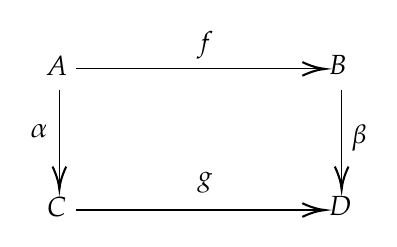
\begin{tikzpicture}[x=0.75pt,y=0.75pt,yscale=-1,xscale=1]
%uncomment if require: \path (0,476); %set diagram left start at 0, and has height of 476

%Straight Lines [id:da7570086255673307] 
\draw    (208,150) -- (326,150) ;
\draw [shift={(328,150)}, rotate = 180] [color={rgb, 255:red, 0; green, 0; blue, 0 }  ][line width=0.75]    (10.93,-3.29) .. controls (6.95,-1.4) and (3.31,-0.3) .. (0,0) .. controls (3.31,0.3) and (6.95,1.4) .. (10.93,3.29)   ;
%Straight Lines [id:da2086758955241419] 
\draw    (336,160) -- (336,206) ;
\draw [shift={(336,208)}, rotate = 270] [color={rgb, 255:red, 0; green, 0; blue, 0 }  ][line width=0.75]    (10.93,-3.29) .. controls (6.95,-1.4) and (3.31,-0.3) .. (0,0) .. controls (3.31,0.3) and (6.95,1.4) .. (10.93,3.29)   ;
%Straight Lines [id:da9244959521459397] 
\draw    (208,218) -- (326,218) ;
\draw [shift={(328,218)}, rotate = 180] [color={rgb, 255:red, 0; green, 0; blue, 0 }  ][line width=0.75]    (10.93,-3.29) .. controls (6.95,-1.4) and (3.31,-0.3) .. (0,0) .. controls (3.31,0.3) and (6.95,1.4) .. (10.93,3.29)   ;
%Straight Lines [id:da04532308225696924] 
\draw    (200,160) -- (200,206) ;
\draw [shift={(200,208)}, rotate = 270] [color={rgb, 255:red, 0; green, 0; blue, 0 }  ][line width=0.75]    (10.93,-3.29) .. controls (6.95,-1.4) and (3.31,-0.3) .. (0,0) .. controls (3.31,0.3) and (6.95,1.4) .. (10.93,3.29)   ;

% Text Node
\draw (193,142.4) node [anchor=north west][inner sep=0.75pt]    {$A$};
% Text Node
\draw (329,142.4) node [anchor=north west][inner sep=0.75pt]    {$B$};
% Text Node
\draw (193,210.4) node [anchor=north west][inner sep=0.75pt]    {$C$};
% Text Node
\draw (329,210.4) node [anchor=north west][inner sep=0.75pt]    {$D$};
% Text Node
\draw (265,130.4) node [anchor=north west][inner sep=0.75pt]    {$f$};
% Text Node
\draw (265,198.4) node [anchor=north west][inner sep=0.75pt]    {$g$};
% Text Node
\draw (185,175.4) node [anchor=north west][inner sep=0.75pt]    {$\alpha $};
% Text Node
\draw (340,175.4) node [anchor=north west][inner sep=0.75pt]    {$\beta $};


\end{tikzpicture}
\end{center}
\end{example}
\begin{definition}
Let $\mathcal{C}$ be a category and $\{A_i:i\in I\}$ a family of objects of $\mathcal{C}$. A \textbf{product} for the family $\{A_i:i\in I\}$ is an object $P$ of $\mathcal{C}$ together with a family of morphisms $\{\pi_i:P\to A_i:i\in I\}$ such that for any object $B$ and family of morphisms $\{\varphi_i:B\to A_i\}$, there is a unique morphism $\varphi:B\to P$ such that $\pi_i\circ\varphi=\varphi_i$ for all $i\in I$.
\end{definition}
We often denote the element $P=\prod_{i\in I}A_i$. We may rephrase the definition of product as that there exists a unique morphism $\varphi:B\to P$, such that the diagram for each $i\in I$
\begin{center}


\tikzset{every picture/.style={line width=0.75pt}} %set default line width to 0.75pt        

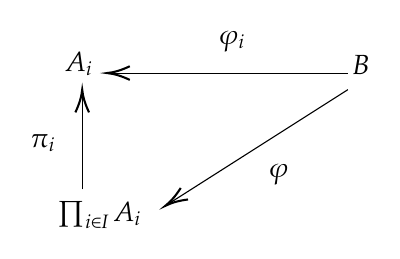
\begin{tikzpicture}[x=0.75pt,y=0.75pt,yscale=-1,xscale=1]
%uncomment if require: \path (0,476); %set diagram left start at 0, and has height of 476

%Straight Lines [id:da7917139115963452] 
\draw    (208,216) -- (208,170) ;
\draw [shift={(208,168)}, rotate = 90] [color={rgb, 255:red, 0; green, 0; blue, 0 }  ][line width=0.75]    (10.93,-3.29) .. controls (6.95,-1.4) and (3.31,-0.3) .. (0,0) .. controls (3.31,0.3) and (6.95,1.4) .. (10.93,3.29)   ;
%Straight Lines [id:da6002607042449972] 
\draw    (336,160) -- (222,160) ;
\draw [shift={(220,160)}, rotate = 360] [color={rgb, 255:red, 0; green, 0; blue, 0 }  ][line width=0.75]    (10.93,-3.29) .. controls (6.95,-1.4) and (3.31,-0.3) .. (0,0) .. controls (3.31,0.3) and (6.95,1.4) .. (10.93,3.29)   ;
%Straight Lines [id:da40319741776590323] 
\draw    (336,168) -- (249.69,222.93) ;
\draw [shift={(248,224)}, rotate = 327.53] [color={rgb, 255:red, 0; green, 0; blue, 0 }  ][line width=0.75]    (10.93,-3.29) .. controls (6.95,-1.4) and (3.31,-0.3) .. (0,0) .. controls (3.31,0.3) and (6.95,1.4) .. (10.93,3.29)   ;

% Text Node
\draw (199,148.4) node [anchor=north west][inner sep=0.75pt]    {$A_{i}$};
% Text Node
\draw (195,220.4) node [anchor=north west][inner sep=0.75pt]    {$\prod _{i\in I} A_{i}$};
% Text Node
\draw (337,150.4) node [anchor=north west][inner sep=0.75pt]    {$B$};
% Text Node
\draw (273,138.4) node [anchor=north west][inner sep=0.75pt]    {$\varphi _{i}$};
% Text Node
\draw (182,188.4) node [anchor=north west][inner sep=0.75pt]    {$\pi _{i}$};
% Text Node
\draw (297,202.4) node [anchor=north west][inner sep=0.75pt]    {$\varphi $};


\end{tikzpicture}
\end{center}
is commute.\par
A family of objects in a category need not have a product. In several familiar categories, however, products always exist. For example, in the category of sets the Cartesian product $\prod_{i\in I}A_i$ is a product of the family $\{A_i:i\in I\}$, which always exist. In the next section we will show that products exist in the category of groups.
\begin{theorem}
If $(P,\{\pi_i\})$ and $(Q,\{\psi_i\})$ are both products of the family $\{A_i:i\in I\}$ of objects of a category $\mathcal{C}$, then $P$ and $Q$ are equivalent.
\end{theorem}
\begin{proof}
Since $P$ and $Q$ are all products of $\{A_i:i\in I\}$, hence there exists morphisms $f$ and $g$ such that the following diagrams 
\begin{center}


\tikzset{every picture/.style={line width=0.75pt}} %set default line width to 0.75pt        

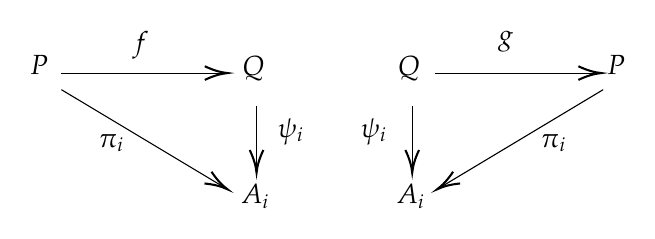
\begin{tikzpicture}[x=0.75pt,y=0.75pt,yscale=-1,xscale=1]
%uncomment if require: \path (0,476); %set diagram left start at 0, and has height of 476

%Straight Lines [id:da7225286591575897] 
\draw    (136,184) -- (214,184) ;
\draw [shift={(216,184)}, rotate = 180] [color={rgb, 255:red, 0; green, 0; blue, 0 }  ][line width=0.75]    (10.93,-3.29) .. controls (6.95,-1.4) and (3.31,-0.3) .. (0,0) .. controls (3.31,0.3) and (6.95,1.4) .. (10.93,3.29)   ;
%Straight Lines [id:da032279626256402905] 
\draw    (230,200) -- (230,230) ;
\draw [shift={(230,232)}, rotate = 270] [color={rgb, 255:red, 0; green, 0; blue, 0 }  ][line width=0.75]    (10.93,-3.29) .. controls (6.95,-1.4) and (3.31,-0.3) .. (0,0) .. controls (3.31,0.3) and (6.95,1.4) .. (10.93,3.29)   ;
%Straight Lines [id:da8049502306412264] 
\draw    (136,192) -- (214.29,238.97) ;
\draw [shift={(216,240)}, rotate = 210.96] [color={rgb, 255:red, 0; green, 0; blue, 0 }  ][line width=0.75]    (10.93,-3.29) .. controls (6.95,-1.4) and (3.31,-0.3) .. (0,0) .. controls (3.31,0.3) and (6.95,1.4) .. (10.93,3.29)   ;
%Straight Lines [id:da6416669281867011] 
\draw    (316,184) -- (394,184) ;
\draw [shift={(396,184)}, rotate = 180] [color={rgb, 255:red, 0; green, 0; blue, 0 }  ][line width=0.75]    (10.93,-3.29) .. controls (6.95,-1.4) and (3.31,-0.3) .. (0,0) .. controls (3.31,0.3) and (6.95,1.4) .. (10.93,3.29)   ;
%Straight Lines [id:da4963797883748118] 
\draw    (305,200) -- (305,230) ;
\draw [shift={(305,232)}, rotate = 270] [color={rgb, 255:red, 0; green, 0; blue, 0 }  ][line width=0.75]    (10.93,-3.29) .. controls (6.95,-1.4) and (3.31,-0.3) .. (0,0) .. controls (3.31,0.3) and (6.95,1.4) .. (10.93,3.29)   ;
%Straight Lines [id:da03213362948006537] 
\draw    (397,192) -- (318.71,238.97) ;
\draw [shift={(317,240)}, rotate = 329.04] [color={rgb, 255:red, 0; green, 0; blue, 0 }  ][line width=0.75]    (10.93,-3.29) .. controls (6.95,-1.4) and (3.31,-0.3) .. (0,0) .. controls (3.31,0.3) and (6.95,1.4) .. (10.93,3.29)   ;

% Text Node
\draw (120,174.4) node [anchor=north west][inner sep=0.75pt]    {$P$};
% Text Node
\draw (222,174.4) node [anchor=north west][inner sep=0.75pt]    {$Q$};
% Text Node
\draw (222,236.4) node [anchor=north west][inner sep=0.75pt]    {$A_{i}$};
% Text Node
\draw (169,162.4) node [anchor=north west][inner sep=0.75pt]    {$f$};
% Text Node
\draw (239,204.4) node [anchor=north west][inner sep=0.75pt]    {$\psi _{i}$};
% Text Node
\draw (153,212.4) node [anchor=north west][inner sep=0.75pt]    {$\pi _{i}$};
% Text Node
\draw (297,174.4) node [anchor=north west][inner sep=0.75pt]    {$Q$};
% Text Node
\draw (398,174.4) node [anchor=north west][inner sep=0.75pt]    {$P$};
% Text Node
\draw (297,236.4) node [anchor=north west][inner sep=0.75pt]    {$A_{i}$};
% Text Node
\draw (279,204.4) node [anchor=north west][inner sep=0.75pt]    {$\psi _{i}$};
% Text Node
\draw (345,162.4) node [anchor=north west][inner sep=0.75pt]    {$g$};
% Text Node
\draw (366,212.4) node [anchor=north west][inner sep=0.75pt]    {$\pi _{i}$};


\end{tikzpicture}
\end{center}
are commute for all $i\in I$. Now by composing these diagrams we get the following diagram:
\begin{center}


\tikzset{every picture/.style={line width=0.75pt}} %set default line width to 0.75pt        

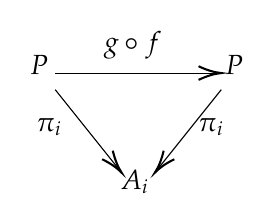
\begin{tikzpicture}[x=0.75pt,y=0.75pt,yscale=-1,xscale=1]
%uncomment if require: \path (0,476); %set diagram left start at 0, and has height of 476

%Straight Lines [id:da4312490537168616] 
\draw    (136,184) -- (214,184) ;
\draw [shift={(216,184)}, rotate = 180] [color={rgb, 255:red, 0; green, 0; blue, 0 }  ][line width=0.75]    (10.93,-3.29) .. controls (6.95,-1.4) and (3.31,-0.3) .. (0,0) .. controls (3.31,0.3) and (6.95,1.4) .. (10.93,3.29)   ;
%Straight Lines [id:da9269323080776339] 
\draw    (136,192) -- (166.75,230.44) ;
\draw [shift={(168,232)}, rotate = 231.34] [color={rgb, 255:red, 0; green, 0; blue, 0 }  ][line width=0.75]    (10.93,-3.29) .. controls (6.95,-1.4) and (3.31,-0.3) .. (0,0) .. controls (3.31,0.3) and (6.95,1.4) .. (10.93,3.29)   ;
%Straight Lines [id:da0759773200651006] 
\draw    (216,192) -- (185.25,230.44) ;
\draw [shift={(184,232)}, rotate = 308.66] [color={rgb, 255:red, 0; green, 0; blue, 0 }  ][line width=0.75]    (10.93,-3.29) .. controls (6.95,-1.4) and (3.31,-0.3) .. (0,0) .. controls (3.31,0.3) and (6.95,1.4) .. (10.93,3.29)   ;

% Text Node
\draw (123,174.4) node [anchor=north west][inner sep=0.75pt]    {$P$};
% Text Node
\draw (217,174.4) node [anchor=north west][inner sep=0.75pt]    {$P$};
% Text Node
\draw (167,229.4) node [anchor=north west][inner sep=0.75pt]    {$A_{i}$};
% Text Node
\draw (158,162.4) node [anchor=north west][inner sep=0.75pt]    {$g\circ f$};
% Text Node
\draw (126,204.4) node [anchor=north west][inner sep=0.75pt]    {$\pi _{i}$};
% Text Node
\draw (204,204.4) node [anchor=north west][inner sep=0.75pt]    {$\pi _{i}$};


\end{tikzpicture}
\end{center}
Thus $g\circ f:P\to P$ is a morphism such that $\pi_i\circ(g\circ f)=\pi_i$ for all $i\in I$. However by definition of a product, we know such morphism is unique and hence $g\circ f=1_P$. Similarly we know that $f\circ g=1_Q$ and hence $f:P\to Q$ is an equivalence.
\end{proof}
Since abstract categories involve only objects and morphisms, every statement about them has a dual statement, obtained by reversing all arrows(morphisms) in the original statement. For example, we know that the product can be state as the commuting diagram as follows:
\begin{center}


\tikzset{every picture/.style={line width=0.75pt}} %set default line width to 0.75pt        

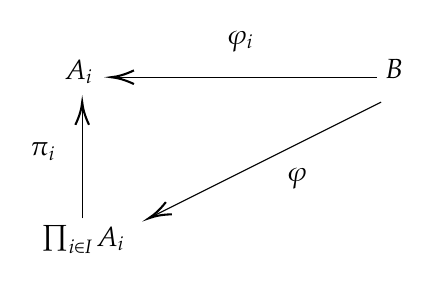
\begin{tikzpicture}[x=0.75pt,y=0.75pt,yscale=-1,xscale=1]
%uncomment if require: \path (0,476); %set diagram left start at 0, and has height of 476

%Straight Lines [id:da2649918540937004] 
\draw    (184,192) -- (184,138) ;
\draw [shift={(184,136)}, rotate = 90] [color={rgb, 255:red, 0; green, 0; blue, 0 }  ][line width=0.75]    (10.93,-3.29) .. controls (6.95,-1.4) and (3.31,-0.3) .. (0,0) .. controls (3.31,0.3) and (6.95,1.4) .. (10.93,3.29)   ;
%Straight Lines [id:da12188979211863638] 
\draw    (326,124) -- (200,124) ;
\draw [shift={(198,124)}, rotate = 360] [color={rgb, 255:red, 0; green, 0; blue, 0 }  ][line width=0.75]    (10.93,-3.29) .. controls (6.95,-1.4) and (3.31,-0.3) .. (0,0) .. controls (3.31,0.3) and (6.95,1.4) .. (10.93,3.29)   ;
%Straight Lines [id:da6877451403419319] 
\draw    (328,136) -- (217.79,191.11) ;
\draw [shift={(216,192)}, rotate = 333.43] [color={rgb, 255:red, 0; green, 0; blue, 0 }  ][line width=0.75]    (10.93,-3.29) .. controls (6.95,-1.4) and (3.31,-0.3) .. (0,0) .. controls (3.31,0.3) and (6.95,1.4) .. (10.93,3.29)   ;

% Text Node
\draw (175,114.4) node [anchor=north west][inner sep=0.75pt]    {$A_{i}$};
% Text Node
\draw (163,194.4) node [anchor=north west][inner sep=0.75pt]    {$\prod _{i\in I} A_{i}$};
% Text Node
\draw (329,114.4) node [anchor=north west][inner sep=0.75pt]    {$B$};
% Text Node
\draw (158,154.4) node [anchor=north west][inner sep=0.75pt]    {$\pi _{i}$};
% Text Node
\draw (253,100.4) node [anchor=north west][inner sep=0.75pt]    {$\varphi _{i}$};
% Text Node
\draw (282,166.4) node [anchor=north west][inner sep=0.75pt]    {$\varphi $};


\end{tikzpicture}
\end{center}
If we reverse all the arrows above, we get another commuting diagram: 
\begin{center}


\tikzset{every picture/.style={line width=0.75pt}} %set default line width to 0.75pt        

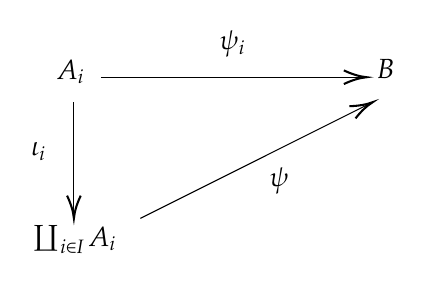
\begin{tikzpicture}[x=0.75pt,y=0.75pt,yscale=-1,xscale=1]
%uncomment if require: \path (0,476); %set diagram left start at 0, and has height of 476

%Straight Lines [id:da2649918540937004] 
\draw    (184,136) -- (184,190) ;
\draw [shift={(184,192)}, rotate = 270] [color={rgb, 255:red, 0; green, 0; blue, 0 }  ][line width=0.75]    (10.93,-3.29) .. controls (6.95,-1.4) and (3.31,-0.3) .. (0,0) .. controls (3.31,0.3) and (6.95,1.4) .. (10.93,3.29)   ;
%Straight Lines [id:da12188979211863638] 
\draw    (197,124) -- (323,124) ;
\draw [shift={(325,124)}, rotate = 180] [color={rgb, 255:red, 0; green, 0; blue, 0 }  ][line width=0.75]    (10.93,-3.29) .. controls (6.95,-1.4) and (3.31,-0.3) .. (0,0) .. controls (3.31,0.3) and (6.95,1.4) .. (10.93,3.29)   ;
%Straight Lines [id:da6877451403419319] 
\draw    (216,192) -- (326.21,136.89) ;
\draw [shift={(328,136)}, rotate = 153.43] [color={rgb, 255:red, 0; green, 0; blue, 0 }  ][line width=0.75]    (10.93,-3.29) .. controls (6.95,-1.4) and (3.31,-0.3) .. (0,0) .. controls (3.31,0.3) and (6.95,1.4) .. (10.93,3.29)   ;

% Text Node
\draw (175,114.4) node [anchor=north west][inner sep=0.75pt]    {$A_{i}$};
% Text Node
\draw (163,194.4) node [anchor=north west][inner sep=0.75pt]    {$\coprod _{i\in I} A_{i}$};
% Text Node
\draw (329,114.4) node [anchor=north west][inner sep=0.75pt]    {$B$};
% Text Node
\draw (162,154.4) node [anchor=north west][inner sep=0.75pt]    {$\iota _{i}$};
% Text Node
\draw (253,100.4) node [anchor=north west][inner sep=0.75pt]    {$\psi _{i}$};
% Text Node
\draw (277,166.4) node [anchor=north west][inner sep=0.75pt]    {$\psi $};


\end{tikzpicture}
\end{center}
From which we give the definition of coproducts:
\begin{definition}
A \textbf{coproduct} (or \textbf{sum}) for the family $\{A_i:i\in I\}$ of objects in a category $\mathcal{C}$ is an object $S$ of $\mathcal{C}$, together with a family of morphisms $\{\iota_i:A_i\to S\}$, such that for any object $B$ and family of morphisms $\{\psi_i:A_i\to B:i\in I\}$, there is a unique morphism $\psi:S\to B$ such that $\psi\circ\iota_i=\psi_i$ for all $i\in I$.
\end{definition}
By the same method used in theorem 2.55 one can proof that the coproduct is unique for a category $\mathcal{C}$. We skip the proof of this proposition.\par
In several of the categories mentioned above, every object in the category is in fact a set (usually with some additional structure) and every morphism in the category is a function on the "underlying sets". We formalize this idea in
\begin{definition}
A \textbf{concrete category} is a category $\mathcal{C}$ together with a function $\sigma$ that assigns to each object $A$ of $\mathcal{C}$ a set $\sigma(A)$(called the \textbf{underlying set} of $A$) in such a way that:\par
(i) every morphism $A\to B$ of $\mathcal{C}$ is a function on the underlying sets $\sigma(A)\to\sigma(B)$;\par
(ii) the identity morphism of each object $A$ of $\mathcal{C}$ is the identity function on the underlying set of $\sigma(A)$;\par
(iii) composition of morphisms in $\mathcal{C}$ agrees with the composition of functions on the underlying sets.
\end{definition}
Indeed, the function $\sigma$ has an effect to "forget" some structures of objects $A$ in the category $\mathcal{C}$. Actually such $\sigma$ is called a \textbf{forgetful functor}.\par
\begin{example}\em
The category of groups $\mathcal{G}$, equipped with the function that assigns to each group its underlying set in the usual sense, is a concrete category.
\end{example}
Concrete categories are frequently useful since one has available not only the properties of a category, but also certain properties of sets, subsets, etc. Since in virtually every concrete category we are interested in, the function $\sigma$ assigns to an object its underlying set in the usual sense, we shall denote both the object and its underlying set by the same symbol and omit any explicit reference to $\sigma$. There is little chance of confusion since we shall be careful in a concrete category $\mathcal{C}$ to distinguish morphisms of $\mathcal{C}$ and maps, which may not be a morphism on $\mathcal{C}$.
\begin{definition}
Let $F$ be an object in a concrete category $\mathcal{C}$. $X$ is a nonempty set, and $i:X\to F$ is a map (of sets). $F$ is \textbf{free on the set $X$} provided that for any object $A$ of $\mathcal{C}$ and map (of sets) $f:X\to A$, there exists a unique morphism $\overline{f}:F\to A$ in $\mathcal{C}$, such that $\overline{f}i=f$ (as a map of sets $X\to A$).
\end{definition}
Also this definition can be rephrased into a commute diagram:
\begin{center}


\tikzset{every picture/.style={line width=0.75pt}} %set default line width to 0.75pt        

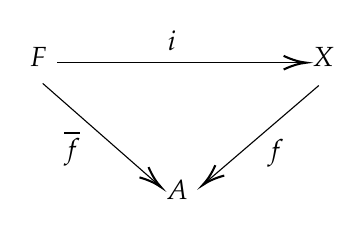
\begin{tikzpicture}[x=0.75pt,y=0.75pt,yscale=-1,xscale=1]
%uncomment if require: \path (0,476); %set diagram left start at 0, and has height of 476

%Straight Lines [id:da3029953557396716] 
\draw    (215,147) -- (333,147) ;
\draw [shift={(335,147)}, rotate = 180] [color={rgb, 255:red, 0; green, 0; blue, 0 }  ][line width=0.75]    (10.93,-3.29) .. controls (6.95,-1.4) and (3.31,-0.3) .. (0,0) .. controls (3.31,0.3) and (6.95,1.4) .. (10.93,3.29)   ;
%Straight Lines [id:da7623644977709794] 
\draw    (341,158) -- (286.52,204.7) ;
\draw [shift={(285,206)}, rotate = 319.4] [color={rgb, 255:red, 0; green, 0; blue, 0 }  ][line width=0.75]    (10.93,-3.29) .. controls (6.95,-1.4) and (3.31,-0.3) .. (0,0) .. controls (3.31,0.3) and (6.95,1.4) .. (10.93,3.29)   ;
%Straight Lines [id:da4655396103461529] 
\draw    (208,157) -- (263.5,205.68) ;
\draw [shift={(265,207)}, rotate = 221.26] [color={rgb, 255:red, 0; green, 0; blue, 0 }  ][line width=0.75]    (10.93,-3.29) .. controls (6.95,-1.4) and (3.31,-0.3) .. (0,0) .. controls (3.31,0.3) and (6.95,1.4) .. (10.93,3.29)   ;

% Text Node
\draw (201,138.4) node [anchor=north west][inner sep=0.75pt]    {$F$};
% Text Node
\draw (337,138.4) node [anchor=north west][inner sep=0.75pt]    {$X$};
% Text Node
\draw (267,202.4) node [anchor=north west][inner sep=0.75pt]    {$A$};
% Text Node
\draw (267,130.4) node [anchor=north west][inner sep=0.75pt]    {$i$};
% Text Node
\draw (315,182.4) node [anchor=north west][inner sep=0.75pt]    {$f$};
% Text Node
\draw (217,178.4) node [anchor=north west][inner sep=0.75pt]    {$\overline{f}$};


\end{tikzpicture}
\end{center}
We will give an example of free objects in section 9, where we will further study some properties of free groups. Now we show an essential fact about a free object $F$, which is, in order to define a morphism with domain $F$, it suffices to specify the image of the subset $i(X)$ as is seen in the following examples.\par
\begin{example}\em
Let $G$ be any group and $g\in G$. Then the map $\overline{f}:\mathbb{Z}\to G$ defined by $\overline{f}(n)=g^n$ is easily to be the unique homomorphism $\mathbb{Z}\to G$ such that $1\mapsto g$. Consequently, if $X=\{1\}$ and $i:X\to\mathbb{Z}$ be the inclusion map, then $\mathbb{Z}$ is free on $X$ in the category of groups. In other words, to determine a unique homomorphism from $\mathbb{Z}$ to $G$, we need only specify the image of $1\in\mathbb{Z}$, which is $i(X)$. 
\end{example}
\begin{theorem}
If $\mathcal{C}$ is a concrete category, $F$ and $F^\prime$ are objects of $\mathcal{C}$ such that $F$ is free on $X$ and $F^\prime$ is free on $X^\prime$, if $|X|=|X^\prime|$, then $F$ and $F^\prime$ are equivalent.
\end{theorem}
\begin{proof}
Since $F$ and $F^\prime$ are free on $X$ and $X^\prime$ separately and $|X|=|X^\prime|$, we may define a bijection $f:X\to X^\prime$ and maps $i:X\to F$, $j:X^\prime\to F^\prime$. Consider the map $jf:X\to F^\prime$. Since $F$ is free on $X$, there exists a morphism $\varphi:F\to F^\prime$ such that the diagram 
\begin{center}


\tikzset{every picture/.style={line width=0.75pt}} %set default line width to 0.75pt        

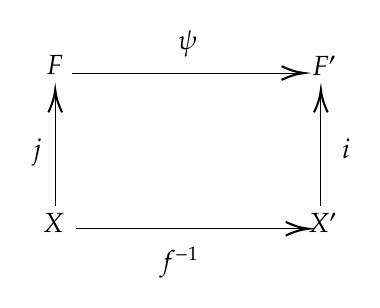
\begin{tikzpicture}[x=0.75pt,y=0.75pt,yscale=-1,xscale=1]
%uncomment if require: \path (0,476); %set diagram left start at 0, and has height of 476

%Straight Lines [id:da9276054517030092] 
\draw    (216,144) -- (326,144) ;
\draw [shift={(328,144)}, rotate = 180] [color={rgb, 255:red, 0; green, 0; blue, 0 }  ][line width=0.75]    (10.93,-3.29) .. controls (6.95,-1.4) and (3.31,-0.3) .. (0,0) .. controls (3.31,0.3) and (6.95,1.4) .. (10.93,3.29)   ;
%Straight Lines [id:da34128781451565393] 
\draw    (208,208) -- (208,154) ;
\draw [shift={(208,152)}, rotate = 90] [color={rgb, 255:red, 0; green, 0; blue, 0 }  ][line width=0.75]    (10.93,-3.29) .. controls (6.95,-1.4) and (3.31,-0.3) .. (0,0) .. controls (3.31,0.3) and (6.95,1.4) .. (10.93,3.29)   ;
%Straight Lines [id:da047714159922908506] 
\draw    (218,219) -- (328,219) ;
\draw [shift={(330,219)}, rotate = 180] [color={rgb, 255:red, 0; green, 0; blue, 0 }  ][line width=0.75]    (10.93,-3.29) .. controls (6.95,-1.4) and (3.31,-0.3) .. (0,0) .. controls (3.31,0.3) and (6.95,1.4) .. (10.93,3.29)   ;
%Straight Lines [id:da6552908409349356] 
\draw    (336,208) -- (336,154) ;
\draw [shift={(336,152)}, rotate = 90] [color={rgb, 255:red, 0; green, 0; blue, 0 }  ][line width=0.75]    (10.93,-3.29) .. controls (6.95,-1.4) and (3.31,-0.3) .. (0,0) .. controls (3.31,0.3) and (6.95,1.4) .. (10.93,3.29)   ;

% Text Node
\draw (201,210.4) node [anchor=north west][inner sep=0.75pt]    {$X$};
% Text Node
\draw (329,210.4) node [anchor=north west][inner sep=0.75pt]    {$X^{\prime }$};
% Text Node
\draw (203,134.4) node [anchor=north west][inner sep=0.75pt]    {$F$};
% Text Node
\draw (331,134.4) node [anchor=north west][inner sep=0.75pt]    {$F^{\prime }$};
% Text Node
\draw (257,226.4) node [anchor=north west][inner sep=0.75pt]    {$f^{-1}$};
% Text Node
\draw (345,174.4) node [anchor=north west][inner sep=0.75pt]    {$i$};
% Text Node
\draw (195,174.4) node [anchor=north west][inner sep=0.75pt]    {$j$};
% Text Node
\draw (266,122.4) node [anchor=north west][inner sep=0.75pt]    {$\psi $};


\end{tikzpicture}
\end{center}
is commutative. Similarly, we have another commute diagram as follow:
\begin{center}


\tikzset{every picture/.style={line width=0.75pt}} %set default line width to 0.75pt        

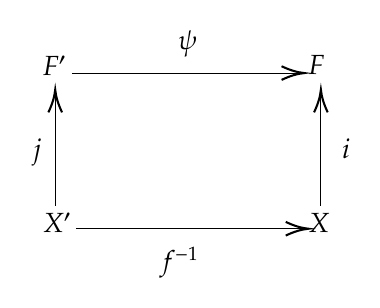
\begin{tikzpicture}[x=0.75pt,y=0.75pt,yscale=-1,xscale=1]
%uncomment if require: \path (0,476); %set diagram left start at 0, and has height of 476

%Straight Lines [id:da9276054517030092] 
\draw    (216,144) -- (326,144) ;
\draw [shift={(328,144)}, rotate = 180] [color={rgb, 255:red, 0; green, 0; blue, 0 }  ][line width=0.75]    (10.93,-3.29) .. controls (6.95,-1.4) and (3.31,-0.3) .. (0,0) .. controls (3.31,0.3) and (6.95,1.4) .. (10.93,3.29)   ;
%Straight Lines [id:da34128781451565393] 
\draw    (208,208) -- (208,154) ;
\draw [shift={(208,152)}, rotate = 90] [color={rgb, 255:red, 0; green, 0; blue, 0 }  ][line width=0.75]    (10.93,-3.29) .. controls (6.95,-1.4) and (3.31,-0.3) .. (0,0) .. controls (3.31,0.3) and (6.95,1.4) .. (10.93,3.29)   ;
%Straight Lines [id:da047714159922908506] 
\draw    (218,219) -- (328,219) ;
\draw [shift={(330,219)}, rotate = 180] [color={rgb, 255:red, 0; green, 0; blue, 0 }  ][line width=0.75]    (10.93,-3.29) .. controls (6.95,-1.4) and (3.31,-0.3) .. (0,0) .. controls (3.31,0.3) and (6.95,1.4) .. (10.93,3.29)   ;
%Straight Lines [id:da6552908409349356] 
\draw    (336,208) -- (336,154) ;
\draw [shift={(336,152)}, rotate = 90] [color={rgb, 255:red, 0; green, 0; blue, 0 }  ][line width=0.75]    (10.93,-3.29) .. controls (6.95,-1.4) and (3.31,-0.3) .. (0,0) .. controls (3.31,0.3) and (6.95,1.4) .. (10.93,3.29)   ;

% Text Node
\draw (329,210.4) node [anchor=north west][inner sep=0.75pt]    {$X$};
% Text Node
\draw (201,210.4) node [anchor=north west][inner sep=0.75pt]    {$X^{\prime }$};
% Text Node
\draw (329,134.4) node [anchor=north west][inner sep=0.75pt]    {$F$};
% Text Node
\draw (201,134.4) node [anchor=north west][inner sep=0.75pt]    {$F^{\prime }$};
% Text Node
\draw (257,226.4) node [anchor=north west][inner sep=0.75pt]    {$f^{-1}$};
% Text Node
\draw (345,174.4) node [anchor=north west][inner sep=0.75pt]    {$i$};
% Text Node
\draw (195,174.4) node [anchor=north west][inner sep=0.75pt]    {$j$};
% Text Node
\draw (266,122.4) node [anchor=north west][inner sep=0.75pt]    {$\psi $};


\end{tikzpicture}
\end{center}
Combining these two diagram together, we have 
\begin{center}


\tikzset{every picture/.style={line width=0.75pt}} %set default line width to 0.75pt        

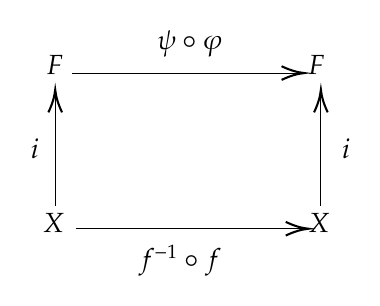
\begin{tikzpicture}[x=0.75pt,y=0.75pt,yscale=-1,xscale=1]
%uncomment if require: \path (0,476); %set diagram left start at 0, and has height of 476

%Straight Lines [id:da9276054517030092] 
\draw    (216,144) -- (326,144) ;
\draw [shift={(328,144)}, rotate = 180] [color={rgb, 255:red, 0; green, 0; blue, 0 }  ][line width=0.75]    (10.93,-3.29) .. controls (6.95,-1.4) and (3.31,-0.3) .. (0,0) .. controls (3.31,0.3) and (6.95,1.4) .. (10.93,3.29)   ;
%Straight Lines [id:da34128781451565393] 
\draw    (208,208) -- (208,154) ;
\draw [shift={(208,152)}, rotate = 90] [color={rgb, 255:red, 0; green, 0; blue, 0 }  ][line width=0.75]    (10.93,-3.29) .. controls (6.95,-1.4) and (3.31,-0.3) .. (0,0) .. controls (3.31,0.3) and (6.95,1.4) .. (10.93,3.29)   ;
%Straight Lines [id:da047714159922908506] 
\draw    (218,219) -- (328,219) ;
\draw [shift={(330,219)}, rotate = 180] [color={rgb, 255:red, 0; green, 0; blue, 0 }  ][line width=0.75]    (10.93,-3.29) .. controls (6.95,-1.4) and (3.31,-0.3) .. (0,0) .. controls (3.31,0.3) and (6.95,1.4) .. (10.93,3.29)   ;
%Straight Lines [id:da6552908409349356] 
\draw    (336,208) -- (336,154) ;
\draw [shift={(336,152)}, rotate = 90] [color={rgb, 255:red, 0; green, 0; blue, 0 }  ][line width=0.75]    (10.93,-3.29) .. controls (6.95,-1.4) and (3.31,-0.3) .. (0,0) .. controls (3.31,0.3) and (6.95,1.4) .. (10.93,3.29)   ;

% Text Node
\draw (201,210.4) node [anchor=north west][inner sep=0.75pt]    {$X$};
% Text Node
\draw (203,134.4) node [anchor=north west][inner sep=0.75pt]    {$F$};
% Text Node
\draw (329,134.4) node [anchor=north west][inner sep=0.75pt]    {$F$};
% Text Node
\draw (247,225.4) node [anchor=north west][inner sep=0.75pt]    {$f^{-1} \circ f$};
% Text Node
\draw (345,174.4) node [anchor=north west][inner sep=0.75pt]    {$i$};
% Text Node
\draw (195,174.4) node [anchor=north west][inner sep=0.75pt]    {$i$};
% Text Node
\draw (256,122.4) node [anchor=north west][inner sep=0.75pt]    {$\psi \circ \varphi $};
% Text Node
\draw (329,210.4) node [anchor=north west][inner sep=0.75pt]    {$X$};


\end{tikzpicture}
\end{center}
Hence $(\psi\circ\varphi)i=i1_X=i$. But $1_Fi=i$, thus by uniqueness of free objects we must have $\psi\circ\varphi=1_F$. A similar argument shows that $\varphi\circ\psi=1_{F^\prime}$. Therefore $F$ is equivalent to $F^\prime$.
\end{proof}
Products, coproducts, and free objects are all defined via \textbf{universal mapping properties}, that is, in terms of the existence of certain uniquely determined morphisms. We formalize the definition as follows:
\begin{definition}
An object $I$ in a category $\mathcal{C}$ is said to be \textbf{universal} (or \textbf{initial}) if for each object $C$ of $\mathcal{C}$ there exists one and only one morphism $I\to C$. An object $T$ in a category $\mathcal{C}$ is said to be \textbf{couniversal} (or \textbf{terminal}) if for each object $C$ of $\mathcal{C}$ there exists one and only one morphism $C\to T$.
\end{definition}
We shall now show that any two universal (couniversal) objects in a category $\mathcal{C}$ are equivalent.
\begin{theorem}
Any two universal (couniversal) objects in a category $\mathcal{C}$ are equivalent.
\end{theorem}
\begin{proof}
Let $I$ and $J$ be universal objects in $\mathcal{C}$. Since $I$ is universal, there is a unique morphism $f:I\to J$. Similarly, there is a unique morphism $g:J\to I$. The composition $g\circ f:I\to I$ is a morphism of $\mathcal{C}$. But $1_I:I\to I$ is also a morphism, then by uniqueness we know that $g\circ f=1_I$. Similarly we have $f\circ g=1_J$ and hence $f$ and $g$ are equivalent. The proof for couniversal objects is analogous.
\end{proof}
Note that categories is a language rather than technique, so we list only a few exercises and we proceed our study for more examples and usage of this language.
\begin{center}
\begin{large}
    \textbf{Exercises for 2.7}
\end{large}
\end{center}
\begin{problem}\em
A pointed set is a pair $(S,x)$ with $S$ a set and $x\in S$. A morphism of pointed sets $(S,x)\mapsto(S^\prime,x^\prime)$ is a triple $(f,x,x^\prime)$ where $f:S\to S^\prime$ is a function satisfies $f(x)=x^\prime$. Show that points sets form a category.
\end{problem}
\begin{proof}
It is clear that for each $(S_1,x_1)$ and $(S_2,x_2)$, the set $\hom((S_1,x_1),(S_2,x_2))$ are disjoint. Also the identity and associativity is trivial. Now we proof that 
$$\hom((S_1,x_1),(S_2,x_2))\times\hom((S_2,x_2),(S_3,x_3))=\hom((S_1,x_1),(S_3,x_3)).$$
To show this, we define the composition $(f,x_1,x_2)\in\hom((S_1,x_1),(S_2,x_2))$ and $(g,x_2,x_3)\in\hom((S_2,x_2),(S_3,x_3))$ as the usual composition of functions, therefore $gf(x_1)=g(x_2)=x_3$ and hence $(gf,x_1,x_3)\in\hom((S_1,x_1),(S_3,x_3))$, which finished our proof.
\end{proof}
\begin{problem}\em
If $f:A\to B$ is an equivalence in a category $\mathcal{C}$ and $g:B\to A$ satisfies $f\circ g=1_B$ and $g\circ f=1_A$, show that $g$ is unique.
\end{problem}
\begin{proof}
Suppose $g$ and $g^\prime$ both satisfy the condition, we proof that $g=g^\prime$. Observed that 
$$
g=1_B\circ g=\left( g^{\prime}\circ f \right) \circ g=g^{\prime}\circ \left( f\circ g \right) =g^{\prime}\circ 1_A=g^{\prime},
$$
hence $g=g^\prime$ and we finished our proof.
\end{proof}
\begin{problem}\em
In the category of groups $\mathcal{G}$, show that the group $G_1\times G_2$ together with the homomorphisms $\pi_1:G_1\times G_2\to G_1$ and $\pi_2:G_1\times G_2\to G_2$ is a product for $\{G_1,G_2\}$.
\end{problem}
\begin{proof}
We first proof that for a class of sets $\{A_i:i\in I\}$ the Cartesian product $\prod_{i\in I}A_i$ is the product in the category $\mathcal{S}$. Let $\pi_i:\prod_{i\in I}A_i\to A_i$, now we show that for an arbitrarily chosen set $C$ and a class of maps $\{\varphi_i:C\to A_i\}$, there exists a unique $\varphi:B\to\prod_{i\in I}A_i$ such that $\varphi_i=\pi_i\circ\varphi$. Let $\varphi$ given by $b\mapsto f_b$, where $f_b(i)=\varphi_i(b)$. It is easy to verify that such $\varphi$ satisfy $\varphi_i=\pi_i\circ\varphi$. Now if there exists another $\varphi^\prime$, observed that 
$$
\varphi ^{\prime}\left( b \right) \left( t \right) =\pi _i\circ \varphi ^{\prime}\left( b \right) =\varphi _i\left( b \right) =f_b\left( i \right) =\varphi \left( b \right) \left( i \right) ,
$$
hence we finished our proof.\par
For this exercise, we simply need to show that $\varphi$ we defined above is a homomorphism, which is easy when observed that 
$$
\varphi \left( ab \right) \left( i \right) =f_{ab}\left( i \right) =\varphi _i\left( ab \right) =\varphi _i\left( a \right) \varphi _i\left( b \right) =f_a\left( i \right) f_b\left( i \right) =\varphi \left( a \right) \varphi \left( b \right) \left( i \right) ,
$$
and hence we finished our proof.
\end{proof}
\begin{problem}\em
Every family $\{A_i:i\in I\}$ in the category of sets has a coproduct.
\end{problem}
\begin{proof}
We define the \textbf{disjoint union} of the set $A_i$ as follows:
$$
\bigsqcup_{i\in I}{A_i}=\left\{ \left( a,i \right) \in \left( \bigcup_{i\in I}{A_i} \right) \times I:a\in A_i \right\} .
$$
Now we define the map $A_i\to\bigsqcup_{i\in I}A_i$ given by $a\mapsto(a,i)$. We proof that $\bigsqcup_{i\in I}{A_i}$ is a coproduct of $\{A_i:i\in I\}$ in the category of sets.\par
For another set $C$ and a class of $\{\psi_i:A_i\to C:i\in I\}$, we define $\psi$ by $(a,i)\mapsto\psi_i(a)$, therefore it is easy to verify that $\psi$ satisfy the condition and unique.
\end{proof}
\subsection{Direct Products and Direct Sums}
In this section we study the product in the category of groups and the coproduct in the category of abelian groups.\par
We begin by extending the definition of the direct product $G\times H$ of groups $G$ and $H$, which we once defined in example 2.3, to an arbitrarily chosen family of groups $\{G_i:i\in I\}$. Define a binary operation on the Cartesian product $\prod_{i\in I}G_i$, which we defined in exercise 2.89. If $f,g\in\prod_{i\in I}G_i$, then $fg$ is given by $i\mapsto f(i)g(i)$. Since $G_i$ is a group, $f(i)g(i)\in G_i$ for all $i\in I$, thence $fg\in\prod_{i\in I}G_i$. $\prod_{i\in I}G_i$, together with the binary operation defined above, is called the \textbf{direct product} of the family of groups $\{G_i:i\in I\}$. If $I$ is finite, we may denote $\prod_{i\in I}G_i=G_1\times G_2\times\cdots\times G_n$. In additive notation, the \textbf{complete direct sum} is denoted as $\bigoplus_{i\in I}G_i$ or $G_1\oplus G_2\oplus\cdots\oplus G_n$ when $I$ is finite. We have shown in exercise 2.89 that $\prod_{i\in I}G_i$ is a product in the category of groups, now we study more properties of direct product.
\begin{proposition}
If $\{G_i:i\in I\}$ is a family of group, then the direct product $\prod_{i\in I}G_i$ is a group, and for each $k\in I$, the map $\pi_k:\prod_{i\in I}G_i\to G_k$ given by $f\mapsto f(k)$ is an epimorphism of groups.
\end{proposition}
\begin{proof}
Clearly for $f,g,h\in\prod_{i\in I}G_i$, $(fg)h=f(gh)$, hence $\prod_{i\in I}G_i$ is a semi-group. Observed that $1\in\prod_{i\in I}G_i$ given by $i\mapsto e_i$, where $e_i$ is the identity element of $G_i$ satisfies $1f=f$, $g1=g$, hence $1$ is the identity element of $\prod_{i\in I}G_i$ and hence a monoid. Now for an arbitrarily chosen $f\in\prod_{i\in I}G_i$, we define $g$ by $i\mapsto(f(i))^{-1}$, which is well-defined since $G_i$ is a group for all $i\in I$. Then $fg=gf=1$, hence $g$ is the inverse of $f$ and $\prod_{i\in I}G_i$ is a group. For each $a\in G_k$, there exists an element $f\in\prod_{i\in I}G_i$ given by $f(k)=a$ and $f(j)=e_j$ where $j\ne k$, hence $\pi_k$ is an epimorphism.
\end{proof}
\begin{note}\em
The map $\pi_k$ here is called the \textbf{canonical projections} of the direct product.
\end{note}
Note that since the direct product of abelian groups is clearly abelian, it follows that the direct product of abelian groups is a product in the category of abelian groups also.\par
\begin{definition}
The \textbf{weak direct product} or the \textbf{external direct product} of a family of groups, denoted as ${\prod}^W_{i\in I}G_i$, is the set of all $f\in\prod_{i\in I}G_i$ such that $f(i)=e_i$, the identity in $G_i$, for all but a finite number of $i\in I$. If all the groups $G_i$ are additive abelian, ${\prod}^W_{i\in I}G_i$ is called the \textbf{external direct sum} and denoted as $\sum_{i\in I}G_i$.
\end{definition}
If $I$ is finite, the weak direct product coincides with the direct product. In any case, we have the following proposition:
\begin{proposition}
If $\{G_i:i\in I\}$ is a family of groups, then\par
(i) ${\prod}^W_{i\in I}G_i$ is a normal subgroup of $\prod_{i\in I}G_i$.\par
(ii) for each $k\in I$, the map $\iota_k:G_k\to{\prod}^W_{i\in I}G_i$ given by $\iota_k(a)=\{a_i\}_{i\in I}$, where $a_i=e$ for $i\ne k$ and $a_k=a$, is a monomorphism of groups.\par
(iii) for each $i\in I$, $\iota_i(G_i)$ is a normal subgroup of $\prod_{i\in I}G_i$.
\end{proposition}
\begin{proof}
(i) Let $f\in{\prod}^W_{i\in I}G_i$ and $f\in\prod_{i\in I}G_i$. Now we consider $gfg^{-1}$, which satisfies $gfg^{-1}(i)=g_if_ig_i^{-1}=g_ig_i^{-1}=e_i$ for all but a finite number of $i$, hence $gfg^{-1}\in{\prod}^W_{i\in I}G_i$ and hence normal in $\prod_{i\in I}G_i$.
(ii) Let $\iota_k(a)=\iota_k(b)$. Therefore the image $\{a_i\}_{i\in I}$ and $\{b_i\}_{i\in I}$ satisfies $a_i=b_i=e$ when $i\ne k$ and $a_k=b_k=a=b$ when $i=k$, hence $a=b$, therefore $\iota_k$ is a monomorphism.\par
(iii) Let $f\in\iota_k(G_k)$ and $g\in\prod_{k\in I}G_k$, therefore 
$$
gfg^{-1}\left( i \right) =g_if_ig_{i}^{-1}=\begin{cases}
	g_ieg_{i}^{-1}=g_ig_{i}^{-1}=e,i\ne k,\\
	g_kf_kg_{k}^{-1}\in G_k,i=k,\\
\end{cases}
$$
hence $gfg^{-1}\in\iota_k(G_k)$ and hence $\iota_k(G_k)\lhd\prod_{i\in I}G_i$.
\end{proof}
\begin{note}\em
The maps $\iota_k$ here is called the \textbf{canonical injection}.
\end{note}
\begin{theorem}
Let $\{A_i:i\in I\}$ be a family of abelian groups written additively. If $B$ is an abelian group and $\{\psi:A_i\to B:i\in I\}$ a family of homomorphisms, then there is a unique homomorphism $\psi:\sum_{i\in I}A_i\to B$ such that $\psi\iota_i=\psi_i$ for all $i\in I$ and this property determine $\sum_{i\in I}A_i$ uniquely up to isomorphism. In other words, $\sum_{i\in I}A_i$ is a coproduct in the category of abelian groups.
\end{theorem}
\begin{proof}
By definition of the external direct sum we know that for each $f\in\sum_{i\in I}A_i$, there is only finite number of $k$ such that $f(k)\ne 0$. We denote such $f(k)$ as $a_k$ and let $\psi(f)=\sum_{k}a_k$. Clearly $\psi$ satisfies the condition $\psi\iota_i=\psi_i$ and it is a homomorphism. Now if $\xi$ is another homomorphism that satisfies $\xi\iota_i=\psi_i$, observed that 
\begin{small}
$$
\xi \left( \left\{ a_i \right\} \right) =\xi \left( \sum_k{\iota _k\left( a \right)} \right) =\sum_k{\xi \iota _k\left( a_k \right)}=\sum_k{\psi _k\left( a_k \right)}=\sum_k{\psi \iota _k\left( a_k \right)}=\psi \left( \sum_k{\iota _k\left( a_k \right)} \right) =\psi \left( \left\{ a_i \right\} \right) ,
$$
\end{small}
hence $\xi=\psi$, which shows that $\psi$ is unique. Therefore $\sum A_i$ is a coproduct in the category of abelian groups and hence is determined up to isomorphism by theorem 2.55 and duality.
\end{proof}
Now we investigate conditions under which a group $G$ is isomorphic to the weak product of a family of its subgroups.
\begin{theorem}
Let $\{N_i:i\in I\}$ be a family of normal subgroups of a group $G$ such that $G=\left<\bigcup_{i\in I}\right>$, and for each $k\in I$, $N_k\cap\left<\bigcup_{i\ne k}\right>=\left<e\right>$. Then $G\cong{\prod}^W_{i\in I}G_i$.
\end{theorem}
\begin{proof}
Let $\{a_i\}\in{\prod}^W_{i\in I}G_i$, then by definition of a weak direct product we know that there are only finite $a_k$ such that $a_k\ne e$. Hence $\{a_i\}=\prod_{k}a_k$. Now we define $\psi:{\prod}^W_{i\in I}G_i\to G$ by $\{a_i\}\mapsto\prod_{k}a_k$. Note that for $a_i\in N_i$ and $a_j\in N_j$ $a_i$ and $a_j$ are commute which we have proved in theorem 2.32, and now we proof that $\psi$ is an isomorphism. First, it is easy to verify that $\psi$ is a homomorphism. Let $a\in G$, by definition of $G$ we may let $a=\prod_{i\in I}a_i$. Now take all $a_k\ne e$ and observed that 
$$
\psi \left( \prod_k{\iota _k\left( a_k \right)} \right) =\prod_k{\psi \iota _k\left( a_k \right)}=\prod_k{a_k}=a,
$$
hence $\psi$ is an epimorphism. Now we show that $\mathrm{Ker}\psi=\left<e\right>$ and hence a monomorphism. Let $\psi \left( \left\{ a_i \right\} \right) =\prod_k{a_k}=e$. Then for all $a_{k_0}$ we have $\prod_k{a_k}=a_{k_0}\prod_{k\ne k_0}{a_k}=e$ and hence 
$$
a_{k_0}^{-1}=\prod_{k\ne k_0}{a_k}\in N_{k_0}\cap \left< \bigcup_{i\ne k_0}{N_i} \right> =\left< e \right> ,
$$
which is $a_{k_0}=e$. Observed that it generally holds and hence $\{a_i\}=e$, therefore $\psi$ is an isomorphism and $G\cong{\prod}^W_{i\in I}G_i$.
\end{proof}
\begin{corollary}
If $N_1,N_2,\cdots,N_r$ are normal subgroups of a group $G$ such that $G=N_1N_2\cdots N_r$ and for each $1\le k\le r$, $N_k\cap(N_1\cdots N_{k-1}N_{k+1}\cdots N_r)=\left<e\right>$, then $G\cong N_1\times N_2\times\cdots\times N_r$.
\end{corollary}
This is an immediate consequence of theorem 2.66 since $I$ can be finite. We skip the proof of this corollary.\par
As another easy corollary of theorem 2.66 we have the following characterization of internal weak direct products.
\begin{theorem}
Let $\{N_i:i\in I\}$ be a family of normal subgroups of a group $G$. $G$ is the internal weak direct product of the family $\{N_iLi\in I\}$ if and only if every non-identity element of $G$ is a unique product $a_{i_1}a_{i_2}\cdots a_{i_n}$ with $i_1,i_2,\cdots,i_n$ distinct elements of $I$ and $e\ne a_{i_k}\in N_{i_k}$ for each $k=1,2,\cdots,n$.
\end{theorem}
\begin{proof}
By theorem 2.66 we know that the internal subgroup of $\{N_i:i\in I\}$ is isomorphic to ${\prod}^W_{i\in I}N_i$, and the theorem immediately follows by the definition of external direct product.
\end{proof}
There are some distinctions between the internal direct product and external direct product. For example, by definition of the internal direct product $G$, each $N_i$ is the subgroup of $G$, then $G$ is isomorphic to ${\prod}^W_{i\in I}N_i$. However, $N_i$ doesn't necessarily be the subgroup of ${\prod}^W_{i\in I}N_i$. In fact, only copies of them are isomorphic to ${\prod}^W_{i\in I}N_i$(namely $\iota_i(N_i)$, we will discuss it later in exercises). Practically speaking, this distinction is not very important and the adjectives "internal" and "external" may be omitted when no confusion is possible to occur.\par
We denote $G={\prod}^w_{i\in I}N_i$ as the internal weak direct product of the family of its subgroups $\{N_i:i\in I\}$.
\begin{theorem}
Let $\{f_i:G_i\to H_i:i\in I\}$ be a family of homomorphisms of groups and let $f=\prod_{i\in I}f_i$ be the map $\prod_{i\in I}G_i\to\prod_{i\in I}H_i$ given by $\{a_i\}\mapsto\{f_i(a_i)\}$. Then $f$ is a homomorphism of groups such that $f\left({\prod}^W_{i\in I}G_i\right)\subset{\prod}^W_{i\in I}H_i$, $\mathrm{Ker}f=\prod_{i\in I}\mathrm{Ker}f_i$ and $\mathrm{Im}f=\prod_{i\in I}\mathrm{Im}f_i$. Consequently $f$ is a monomorphism [resp. epimorphism] if and only if each $f_i$ is.
\end{theorem}
\begin{proof}
We first proof that $f$ is a homomorphism, which only need to observe that 
$$
f\left( \left\{ a_ib_i \right\} \right) =f_i\left( a_ib_i \right) =f_i\left( a_i \right) f_i\left( b_i \right) =f\left( \left\{ a_i \right\} \right) f\left( \left\{ b_i \right\} \right) .
$$
Now it is trivial that $f\left({\prod}^W_{i\in I}G_i\right)\subset{\prod}^W_{i\in I}H_i$ and we show $\mathrm{Ker}f=\prod_{i\in I}\mathrm{Ker}f_i$, $\mathrm{Im}f=\prod_{i\in I}\mathrm{Im}f_i$. In fact, if $\{a_i\}\in\prod_{i\in I}\mathrm{Ker}f_i$, then $f\left( \left\{ a_i \right\} \right) =\left\{ f_i\left( a_i \right) \right\} =\left< e \right> $ and hence $\mathrm{Ker}f\supset \prod_{i\in I}{\mathrm{Ker}f_i}$. Conversely, if $\{a_i\}\in\mathrm{Ker}f$, then $f\left( \left\{ a_i \right\} \right) =\left\{ f_i\left( a_i \right) \right\} =\left< e \right> $ for all $i\in I$, whence $\left\{ a_i \right\} \in \prod_{i\in I}{\mathrm{Ker}f_i}$. Hence $\mathrm{Ker}f=\prod_{i\in I}\mathrm{Ker}f_i$. Similarly one may verify that $\mathrm{Im}f=\prod_{i\in I}\mathrm{Im}f_i$.
\end{proof}
\begin{corollary}
Let $\{G_i:i\in I\}$ and $\{N_i:i\in I\}$ be two families of groups such that $N_i\lhd G_i$ for each $i\in I$.\par
(i)$\prod_{i\in I}{N_i}\lhd \prod_{i\in I}{G_i}$ and $\prod_{i\in I}{G_i}/\prod_{i\in I}{N_i}\cong \prod_{i\in I}{\left( G_i/N_i \right)}$.\par
(ii)${\prod}^W_{i\in I}{N_i}\lhd {\prod}^W_{i\in I}{G_i}$ and ${\prod}^W_{i\in I}{G_i}/{\prod}^W_{i\in I}{N_i}\cong {\prod}^W_{i\in I}{\left( G_i/N_i \right)}$.
\end{corollary}
\begin{proof}
We only proof (i) and (ii) can be proved similarly.\par
Define the canonical epimorphism $\pi_i:G_i\to G_i/N_i$. Then the product $\pi =\prod_{i\in I}{\pi _i}:\prod_{i\in I}{G_i}\rightarrow \prod_{i\in I}{\left( G_i/N_i \right)}$ is an epimorphism with kernel $\mathrm{Ker}\pi=\prod_{i\in I}N_i$. Hence by the First Isomorphism Theorem we have $\prod_{i\in I}{N_i}\lhd \prod_{i\in I}{G_i}$ and $\prod_{i\in I}{G_i}/\prod_{i\in I}{N_i}\cong \prod_{i\in I}{\left( G_i/N_i \right)}$.
\end{proof}
\begin{center}
\begin{large}
    \textbf{Exercises for 2.8}
\end{large}
\end{center}
\begin{problem}\em
Show that $S_3$ is not the direct product of any family of its proper groups. The same is true for $\mathbb{Z}_{p^n}$ and $\mathbb{Z}$.
\end{problem}
\begin{proof}
Our proof depend on an observation that if $A$ and $B$ are abelian, then so is $A\times B$. Now we consider the subgroups of $S_3$. By Lagrange's Theorem, it has an order either $2$ or $3$, which are all prime. Hence subgroups of $S_3$ are all abelian, so if $S_3$ is the direct product of some of its subgroups, it must be abelian, which is a contradiction!\par
The proof for $\mathbb{Z}_{p^n}$ is similar since $\mathbb{Z}_{p^n}$ has its subgroups of the form $\left<p^k\right>$ where $1\le k\le n-1$. Consider any product $\left<p^i\right>\times\left<p^j\right>$. Let $G=\mathbb{Z}_{p^{i_1}}\times\mathbb{Z}_{p^{i_2}}\times\cdots\times\mathbb{Z}_{p^{i_m}}$, then both $\left<(p^{i-1},0,\cdots,0)\right>$ and $\left<(0,0,\cdots,p^{j-1})\right>$ are both subgroups with order $p$. However, this can't be true since by exercise 2.35 we know that such subgroup should be unique. Therefore $G$ is not the internal subgroup of $\mathbb{Z}_{p^n}$.\par
The group $\mathbb{Z}$ is cyclic. However, any product of its subgroups contains a subgroup $m\mathbb{Z}\times n\mathbb{Z}$, which is not cyclic. Hence $\mathbb{Z}$ is not the direct product of some of its subgroups by the same reason.
\end{proof}
\begin{problem}\em
Give an example of groups $H_i,K_j$ such that $H_1\times H_2\cong K_1\times K_2$, but $H_i\not\cong K_j$ for any $i,j=1,2$.
\end{problem}
\begin{proof}
Consider the example $\mathbb{Z}_2\times\mathbb{Z}_6$ and $(\mathbb{Z}_2\times\mathbb{Z}_2)\times\mathbb{Z}_3$. We first show that $\mathbb{Z}_2\times\mathbb{Z}_6\cong(\mathbb{Z}_2\times\mathbb{Z}_2)\times\mathbb{Z}_3$. Observed that the element $(1,1)\in\mathbb{Z}_2\times\mathbb{Z}_3$ generates the whole $\mathbb{Z}_2\times\mathbb{Z}_3$, therefore $\mathbb{Z}_2\times\mathbb{Z}_3\cong\mathbb{Z}_6$. Now define the map $(0,1)\mapsto((0,1)),0$ and $(1,0)\mapsto((1,0),0)$. Since the generators determined the whole map, we know that it is an isomorphism. However, no isomorphism exists in $\mathbb{Z}_2,\mathbb{Z}_6,\mathbb{Z}_2\times\mathbb{Z}_2$ and $\mathbb{Z}_3$.
\end{proof}
\begin{note}\em
This example shows that the decomposition of a group may not be unique.
\end{note}
\begin{problem}\em
Let $G$ be an additive abelian group with subgroups $H$ and $K$. Show that $G\cong H\oplus K$ if and only if there are homomorphisms $H\underset{\iota _1}{\overset{\pi _1}{\leftrightarrows}}G\underset{\iota _2}{\overset{\pi _2}{\leftrightarrows}}K$ such that $\pi_1\iota_1=1_H,\pi_2\iota_2=1_K,\pi_1\iota_2=0$ and $\pi_2\iota_1=0$, where $0$ is the map sending every element onto zero element, and $\iota_1\pi_1(x)+\iota_2\pi_2(x)=x$ for all $x\in G$.
\end{problem}
\begin{proof}
If $G\cong H\oplus K$, then for all $x\in G$, we may write $x=(h,k)$ where $h\in H$ and $k\in K$. Hence we define $\pi_1:(h,k)\mapsto h,\pi_2:(h,k)\mapsto k$ and $\iota_1:h\mapsto(h,0),\iota_2:k\mapsto(0,k)$, then it is easy to verify that these maps are homomorphisms and satisfy the condition shown in exercise. Conversely, since $\pi_1\iota_1=1_H$, we know that $\iota_1$ is injective and $\pi_1$ is surjective. Hence $H$ is embedded in $G$, that is, $H^\prime=\iota_1(H)<G$. Given $h^\prime\in H^\prime$, there is a unique $h\in H$ such that $\iota_1(h)=h^\prime$, hence $H\cong H^\prime$. Similarly we have $K\cong H^\prime$. Now that $\iota_1\pi_1(x)+\iota_2\pi_2(x)=x$ hence $G=H^\prime+K^\prime$. We define $f:G\to H\oplus K$ by $h^\prime+k^\prime\mapsto(h,k)$, which is easy to see is an isomorphism, hence $G\cong H\oplus H$.
\end{proof}
\begin{problem}\em
Let $G,H$ be cyclic groups. Then $G\times H$ is cyclic if and only if $(|G|,|H|)=1$.
\end{problem}
\begin{proof}
If $G\times H$ is cyclic but $(|G|,|H|)\ne 1$. Then we may take elements from $G$ and $H$, denote $g,h$, have the same order. Now consider $G\times H$. Since $(g,e_H)$ and $(e_G,h)$ are both elements of $G\times H$, then $\left<(g,e_H\right>$ and $\left<e_G,h\right>$ have the same order and all subgroups of $G\times H$, which contradicts to the fact that $G\times H$ is cyclic. Conversely, if $(|G|,|H|)=1$, then suppose $|G|=p$ and $|H|=q$, we know by exercise 2.31 that $G\times H$ is an abelian group that contains an element of order $[m,n]$. Observed that $mn=[m,n](m,n)=[m,n]$ and $|G\times H|=|G|\times|H|=mn$, we know that $G\times H$ is cyclic since it can be generated by one element.
\end{proof}
\begin{problem}\em
Every finite generated abelian group $G\ne\left<e\right>$ in which every element (except $e$) has order $p$ ($p$ prime) is isomorphic to $\mathbb{Z}_p\oplus\mathbb{Z}_p\oplus\cdots\oplus\mathbb{Z}_p$.
\end{problem}
\begin{proof}
Let $A=\{a_1,a_2,\cdots,a_n\}$ be the collection of all generators of $G$, which satisfy $\left< A\setminus \left\{ a_k \right\} \right> \ne G$ for all $k\in\{1,2,\cdots,n\}$. Denote $\left<a_k\right>=N_k$, then $N_k\lhd G$. We now show that $G$ is the direct product of $N_k,k=1,2,\cdots,n$. First observed that 
$A\subset (N_1\cup N_2\cup \cdots \cup N_n)$, hence $G\subset \left< N_1\cup N_2\cup \cdots \cup N_n \right> $. The converse condition is trivial and hence $G=\left< N_1\cup N_2\cup \cdots \cup N_n \right> $. Now we show that 
$$N_k\cap \left( N_1\cup \cdots \cup N_{k-1}\cup N_{k+1}\cup \cdots \cup N_n \right) =0$$ 
for all $k\in\{1,2,\cdots,n\}$. Observed that 
$$N_k\cap \left( N_1\cup \cdots \cup N_{k-1}\cup N_{k+1}\cup \cdots \cup N_n \right) $$
is the subset of $N_k$ and $N_k$ has an order $p$, which is prime, therefore 
$$N_k\cap \left( N_1\cup \cdots \cup N_{k-1}\cup N_{k+1}\cup \cdots \cup N_n \right) =N_k\ \text{or}\ 0.$$
If the first, $\left< N_1\cup \cdots \cup N_{k-1}\cup N_{k+1}\cup \cdots \cup N_n \right> $ generates the whole $G$, which contradict to the definition of $A$. Hence $N_k\cap \left( N_1\cup \cdots \cup N_{k-1}\cup N_{k+1}\cup \cdots \cup N_n \right) =0 $ and therefore we finished our proof.
\end{proof}
\begin{problem}\em
Let $H,K,N$ be nontrivial normal subgroups of a group $G$ and suppose $G=H\times K$. Prove that $N$ is in the center of $G$ or $N$ intersects one of $H,K$ nontrivially. Give examples to show that both possibilities can actually occur when $G$ is not abelian.
\end{problem}
\begin{proof}
Suppose $N\cap H=N\cap K=\left<e\right>$. Now take $n\in N$ and $k\in K$. Since $N$ is normal in $G$, we know that $knk^{-1}\in N$. Also we know that $nk^{-1}n^{-1}\in K$ since $k$ is normal in $G$. This shows that $knk^{-1}n^{-1}\in N\cap K=\left<e\right>$ and hence $kn=nk$. Similarly we have $hn=nh$ and therefore $Z(G)=G$, we finished our proof.\par
Now we give an example that both two condition may be true when $G$ is not abelian. Consider $D_2\cong\mathbb{Z}_2\oplus\mathbb{Z}_2$. We denote $D_2=\left<a\right>\times\left<b\right>$ and it has a subgroup $\left<ab\right>$ which does not intersect either product. However, since the group is abelian then every element is contained in the center. Then consider $D_6$. We observed that $D_6=\left<a^3\right>\times\left<a^2,b\right>\cong\mathbb{Z}_2\oplus D_3$, where $\left<a^3\right>\cap\left<a^2,b\right>=\left<e\right>$.
\end{proof}
\begin{problem}\em
Corollary 2.67 is false if one of the $N_i$ is not normal.
\end{problem}
\begin{problem}\em
If a group $G$ is the (internal) direct product of its subgroups $H,K$, then $H\cong G/K$ and $K\cong G/H$.
\end{problem}
\begin{proof}
Consider the canonical projection $\pi_H:G\to H$ and $\pi_K:G\to K$. We have shown that $\mathrm{Ker}\pi_K=H$, therefore by the First Isomorphism Theorem we have $G/\mathrm{Ker}\pi_K\cong\mathrm{Im}\pi_K$. However, it is easy to verify $\pi_K$ is an epimorphism and hence $\mathrm{Im}\pi_K=K$, therefore $G/H\cong K$. Analogously we have $G/K\cong H$.
\end{proof}
\begin{problem}\em
If $\{G_i:i\in I\}$ is a family of groups, then ${\prod}^w_{i\in I}G_i$ is the internal weak product of its subgroups $\{\iota_i(G_i):i\in I\}$.
\end{problem}
\begin{proof}
We have shown that $\iota_i(G_i)$ is normal in ${\prod}^w_{i\in I}G_i$. Now we show that 
$$
\iota _i\left( G_i \right) \cap \left( \iota _1\left( G_1 \right) \cup \cdots \cup \iota _{i-1}\left( G_{i-1} \right) \cup \iota _{i+1}\left( G_{i+1} \right) \cup \cdots \cup \iota _n\left( G_n \right) \right) =\left< e \right> .
$$
In fact we know that the map $\iota _i:G_i\rightarrow {\prod}^w_{i\in I}{G_i}$ is an embedding that 
$$\iota _i\left( G_i \right) =\left( e_1,\cdots ,e_{i-1},G_i,e_{i+1},\cdots ,e_n \right) ,$$
hence
$$
\iota _i\left( G_i \right) \cap \left( \iota _1\left( G_1 \right) \cup \cdots \cup \iota _{i-1}\left( G_{i-1} \right) \cup \iota _{i+1}\left( G_{i+1} \right) \cup \cdots \cup \iota _n\left( G_n \right) \right) =\left< e \right> .
$$
Then the statement follows by the fact that $
{\prod}^w_{i\in I}{G_i}=\left< \bigcup_{i\in I}{\iota _i\left( G_i \right)} \right> $.
\end{proof}
\begin{problem}\em
Let $\{N_i:i\in I\}$ is a family of subgroups of a group $G$. Then $G$ is the internal weak product of $\{N_i:i\in I\}$ if and only if:\par
(i) $a_ia_j=a_ja_i$ for all $i\ne j$ and $a_i\in N_i,a_j\in N_j$.\par
(ii) every non-identity element of $G$ is uniquely a product $a_{i_1}\cdots a_{i_n}$, where $i_1,i_2,\cdots,i_n$ are distinct elements of $I$ and $e\ne a_{i_k}$ for each $k$.
\end{problem}
\begin{proof}
By definition of an internal weak direct product we know that each $N_i$ is the normal subgroup of $G$. Then the statement immediately follows by theorem 2.32 and theorem 2.68. Conversely, by theorem 2.68 it suffices to show that each $N_i$ is normal in $G$, which is trivial when observed that for all $n_i\in N_i$ and $g\in G$, by (ii) we write $g=a_{i_1}\cdots a_{i_k}$, we have 
$$
gn_ig^{-1}=n_{i_1}n_{i_2}\cdots n_{i_n}n_in_{i_n}^{-1}n_{i_{n-1}}^{-1}\cdots n_{i_1}^{-1}=\left( n_{i_1}n_{i_1}^{-1} \right) \left( n_{i_2}n_{i_2}^{-1} \right) \cdots \left( n_{i_n}n_{i_n}^{-1} \right) n_i=n_i\in N_i,
$$
by which we finished our proof.
\end{proof}
\begin{problem}\em
Let $\{G_i:i\in I\}$ be a family of groups and $J\subset I$. The map $\alpha:\prod_{j\in J}G_j\to\prod_{i\in I}G_i$ given by $\{a_i\}\mapsto\{b_i\}$, where $b_j=a_j$ for $j\in J$ and $b_i=e_i$ for $i\notin J$, is a monomorphism of groups and $\prod_{i\in I}G_i/\alpha\left(\prod_{j\in J}G_j\right)\cong\prod_{i\in I\setminus J}G_i$.
\end{problem}
\begin{proof}
It is easy to verify that $\alpha$ is a monomorphism, we now proof $\prod_{i\in I}G_i/\alpha\left(\prod_{j\in J}G_j\right)\cong\prod_{i\in I\setminus J}G_i$. Define $\beta :\prod_{i\in I}{G_i}\rightarrow \prod_{i\in I\setminus J}{G_i}$ by $\{a_i\}\mapsto e$ if $\{a_i\}\in\prod_{j\in J}G_j$, otherwise $\{a_i\}\mapsto\{a_i\}$. It is easy to verify that $\beta$ is a homomorphism and $\mathrm{Ker}\beta=\alpha\left(\prod_{i\in I}G_i\right)$. Therefore by the First Isomorphism Theorem we have $\prod_{i\in I}G_i/\alpha\left(\prod_{j\in J}G_j\right)\cong\prod_{i\in I\setminus J}G_i$.
\end{proof}
\subsection{Free Groups, Free Products, Generators and Relations}
We shall show that free objects exists in the category of groups, and we shall use these to develop a method of describing groups in terms of "generators and relations". In addition, we indicate how to construct coproduct (free product) in the category of groups.\par
We now construct a free group on a given group $X$. If $X=\emptyset$, then $F$ is trivially $\left<e\right>$. Otherwise we consider the sequence $x_1x_2\cdots x_n\in F$, here $x_i\in X,i=1,2,\cdots,n$. In order $F$ to be a group, there must be an inverse for such an element in $F$. Hence we define a set $X^{-1}$ disjoint from $X$, such that $|X|=|X^{-1}|$. Hence there is a bijection $x\mapsto x^{-1}$ from $X$ to $X^{-1}$. Now choose an element $1$ out of $X\cup X^{-1}$. We say the sequence $x_1x_2\cdots x_n\cdots$ is a \textbf{word}, if there exists an index $k$ such that $a_j=1$ when $j\ge k$. The constant sequence $11\cdots1\cdots$ is denoted as $1$. A word $x_1x_2\cdots x_n$ is \textbf{reduced}, if \par
(i) for all $x\in X$, $x$ and $x^{-1}$ are not adjacent. That is, if $x_k=x$, then $x_{k+1}\ne x^{-1}$ and vice versa.\par
(ii) $a_k=1$ implies $a_j=1$ for all $j\ge k$.\par
Every reduced word has the form $x_1^{\lambda_1}x_2^{\lambda_2}\cdots x_n^{\lambda_n}$, where $x_i\in X$ and $\lambda_i=1$ or $-1$. Observed that $x_{1}^{\delta _1}x_{2}^{\delta _2}\cdots x_{n}^{\delta _n}=y_{1}^{\lambda _1}y_{2}^{\lambda _2}\cdots y_{m}^{\lambda _m}$ if and only if $m=n$, $x_i=y_i$ and $\delta_i=\lambda_i$. We now define the binary product as follows (in order that the product of two reduced words is reduced):
$$
\left( x_{1}^{\delta _1}x_{2}^{\delta _2}\cdots x_{n}^{\delta _n} \right) \left( y_{1}^{\lambda _1}y_{2}^{\lambda _2}\cdots y_{m}^{\lambda _m} \right) =\begin{cases}
	x_{1}^{\delta _1}x_{2}^{\delta _2}\cdots x_{n-k}^{\delta _{n-k}}y_{k+1}^{\lambda _{k+1}}y_{k+2}^{\lambda _{k+2}}\cdots y_{m}^{\lambda _m},k<m,\\
	y_{n+1}^{\lambda _{n+1}}y_{n+2}^{\lambda _{n+2}}\cdots y_{m}^{\lambda _m},k=m<n,\\
	1,k=m=n,\\
\end{cases}
$$
here $k$ is the largest integer such that $x_{n-j}^{\delta_{m-j}}=y_{j+1}^{-\lambda_{j+1}}$ for $j=1,2,\cdots,k-1$.
\begin{theorem}
If $X$ is a nonempty set and $F=F(X)$ is the set of all reduced words on $X$, then $F$ is a group under the binary operation defined above and $F=\left<X\right>$.
\end{theorem}
\begin{proof}
By definition of $F$ we know that $F$ has an identity element $1$ and for each $w\in F$ there is an inverse element $w^{-1}$. Now we show that elements in $F$ is associative. For each $x\in X$ and $\delta=-1$ or $1$, we define the map $|x^\delta|:F\to F$ given by 
$$
\left| x^{\delta} \right|\left( x_{1}^{\delta _1}x_{2}^{\delta _2}\cdots x_{n}^{\delta _n} \right) =\begin{cases}
	x^{\delta}x_{1}^{\delta _1}x_{2}^{\delta _2}\cdots x_{n}^{\delta _n},x^{\delta}x_{1}^{\delta _1}\ne 1,\\
	x_{2}^{\delta _2}\cdots x_{n}^{\delta _n},x^{\delta}x_1^{\delta_1}=1,\\
\end{cases}
$$
Since $|x||x^{-1}|=|x^{-1}||x|=1_F$, we know that every $|x^\delta|$ is a permutation of $F$. Let $F_0$ be the subgroup generated by $\{|x|:x\in X\}$. Now we define a map $\varphi:F\to F_0$ by $1\mapsto 1_F$ and $x_{1}^{\delta _1}x_{2}^{\delta _2}\cdots x_{n}^{\delta _n}\mapsto \left| x_{1}^{\delta _1} \right|\left| x_{2}^{\delta _2} \right|\cdots \left| x_{n}^{\delta _n} \right|$. We first show that it is a homomorphism. Observed that 
$$
\varphi \left( w_1w_2 \right) =\left| w_1w_2 \right|=\left| w_1 \right|\left| w_2 \right|=\varphi \left( w_1 \right) \varphi \left( w_2 \right) 
$$
hence $\varphi$ is a homomorphism. Clearly $\varphi$ is surjective. Then by definition of $\varphi$ that $1\mapsto 1_F$, hence $\mathrm{Ker}\varphi=1$ and hence injective. Therefore $\varphi$ is an isomorphism and hence $F\cong F_0$. Elements in $F_0$ is associative since $F_0$ is a group, therefore elements in $F$ is associative and we finished our proof.
\end{proof}
\begin{note}\em
The proof method above is called the \textbf{van der Waerden trick}.
\end{note}
\begin{definition}
The group $F=F(X)$ is called the \textbf{free group on the set $X$}.
\end{definition}
Here we explain the terminology "free".
\begin{theorem}
Let $F$ be the free group on a set $X$ and $\iota:X\to F$ is the inclusion map. If $G$ is a group and $f:X\to G$ a map of sets, then there exists a unique homomorphism of groups $\overline{f}:F\to G$ such that $\overline{f}\iota=f$.
\end{theorem}
\begin{proof}
We define the map $\overline{f}:F\to G$ by $\overline{f}(1)=e_G$ and 
$$\overline{f}\left( x_{1}^{\delta _1}x_{2}^{\delta _2}\cdots x_{n}^{\delta _n} \right) =f^{\delta _1}\left( x_1 \right) f^{\delta _2}\left( x_2 \right) \cdots f^{\delta _n}\left( x_n \right) .$$
We first proof that $\overline{f}$ is a homomorphism. Observed that 
$$
\begin{aligned}
\overline{f}\left( x_{1}^{\delta _1}x_{2}^{\delta _2}\cdots x_{n}^{\delta _n}y_{1}^{\lambda _1}y_{2}^{\lambda _2}\cdots y_{m}^{\lambda _m} \right) &=f^{\delta _1}\left( x_1 \right) f^{\delta _2}\left( x_2 \right) \cdots f^{\delta _n}\left( x_n \right) f^{\lambda _1}\left( y_1 \right) f^{\lambda _2}\left( y_2 \right) \cdots f^{\lambda _m}\left( y_m \right) \\
&=\overline{f}\left( x_{1}^{\delta _1}x_{2}^{\delta _2}\cdots x_{n}^{\delta _n} \right) \overline{f}\left( y_{1}^{\lambda _1}y_{2}^{\lambda _2}\cdots y_{m}^{\lambda _m} \right) ,
\end{aligned}
$$
hence $\overline{f}$ is a homomorphism. Now we show that $\overline{f}\iota=f$, which we observed that for all $x\in X$, $\iota(x)=x$, hence $\overline{f}\iota(x)=\overline{f}(x)=f(x)$, therefore $\overline{f}\iota=f$. Now if there is another homomorphism $g$ such that $g\iota=f$, we show that $g=\overline{f}$ by 
$$
\begin{aligned}
g\left( x_{1}^{\delta _1}x_{2}^{\delta _2}\cdots x_{n}^{\delta _n} \right) &=g\left( x_{1}^{\delta _1} \right) g\left( x_{2}^{\delta _2} \right) \cdots g\left( x_{n}^{\delta _n} \right)\\
&=g^{\delta _1}\left( x_1 \right) g^{\delta _2}\left( x_2 \right) \cdots g^{\delta _n}\left( x_n \right)=g\iota ^{\delta _1}\left( x_1 \right) g\iota ^{\delta _2}\left( x_2 \right) \cdots g\iota ^{\delta _n}\left( x_n \right)\\
&=f^{\delta _1}\left( x_1 \right) f^{\delta _2}\left( x_2 \right) \cdots f^{\delta _n}\left( x_n \right) =\overline{f}\left( x_{1}^{\delta _1}x_{2}^{\delta _2}\cdots x_{n}^{\delta _n} \right) ,
\end{aligned}
$$
hence we finished our proof.
\end{proof}
\begin{note}\em
In other words, $F$ is a free object on the set $X$ in the category of groups.
\end{note}
\begin{corollary}
Every group $G$ is isomorphic to quotient group of a free group.
\end{corollary}
\begin{proof}
By theorem 2.73 we know that the map $\overline{f}$ is an epimorphism, hence by the First Isomorphism Theorem we know that $G\cong F/\mathrm{Ker}\overline{f}$.
\end{proof}
By corollary 2.74 we know that in order to determine a group $G$, it suffices to determine $F,X$ and $\mathrm{Ker}\overline{f}=N$. However $F$ is determined up to isomorphism by $X$, and $N$ is determined by the homomorphism $\mathrm{Ker}\overline{f}$. Now if $w=x_1^{\delta_1}x_2^{\delta_2}\cdots x_n^{\delta_n}$ is a generator of $N$, then under the epimorphism $x_1^{\delta_1}x_2^{\delta_2}\cdots x_n^{\delta_n}=e$. We call the equation $x_1^{\delta_1}x_2^{\delta_2}\cdots x_n^{\delta_n}=e$ a \textbf{relation} of generators $x_i$ on $G$. Clearly a group can be determined by a set $X$ of generators and a suitable set $R$ of relations. This description is not unique, since there are many choices of $X$ and $R$.\par
Conversely, we may ask given a set $X$ and $Y$ of reduced words on the element of $X$, does there exists a group $G$ such that $G$ is generated by $X$ and the relations $w=e,w\in Y$ are all valid? We will see that the statement is true, providing one allows for the possibility that in the group $G$ the elements of $X$ may not all be distinct. For example, let $a,b\in X$ and $ab^{-1}\in Y$. Then every group $G$ containing $a$ and $b$ and satisfying $ab^{-1}=e$ must have $a=b$.\par
We now construct the group as follows. Let $F$ be the free group on $X$ and $N$ be the normal group generated by $Y$ (which is the intersection of all normal groups in $F$ that contains $Y$). Let $G$ be the quotient group $F/N$ and identify $X$ with its image in $F/N$ under the map $X\subset F\to F/N$. Then $G$ is a group generated by $X$ and for all $w\in Y$, 
$$
w=x_{1}^{\delta _1}x_{2}^{\delta _2}\cdots x_{n}^{\delta _n}\in Y\Rightarrow x_{1}^{\delta _1}x_{2}^{\delta _2}\cdots x_{n}^{\delta _n}\in N\Rightarrow x_{1}^{\delta _1}Nx_{2}^{\delta _2}N\cdots x_{n}^{\delta _n}N=N,
$$
hence $w=e$ in $G$.\par
\begin{definition}
Let $X$ be a set and $Y$ be a set of reduced words on $X$. A group $G$ is said to be the \textbf{group defined by the generators $x\in X$ and relations $w=e(w\in Y)$} provided $G\cong F/N$, where $F$ is the free group of $X$ and $N$ be the normal subgroup of $F$ generated by $Y$. One says that $(X\mid Y)$ is the \textbf{presentation} of $G$.
\end{definition}
The preceding discussion shows that the group defined by given generators and relations always exists. Furthermore it is the largest possible such group in the following sense.
\begin{theorem}(Van Dyck)
Let $X$ be a set, $Y$ a set of reduced words on $X$ and $G$ the group defined by the generators $x\in X$ and relations $w=e,w\in Y$. If $H$ is any group such that $H=\left<X\right>$ and $H$ satisfies all the relations $w=e(w\in Y)$, then there is an epimorphism $G\to H$.
\end{theorem}
\begin{note}\em
The elements of $Y$ are being interpreted as words in $X$, products in $G$ and products in $H$ as the context indicates.
\end{note}
\begin{proof}
If $F$ is the free group on $X$ then the inclusion map $X\to H$ induces an epimorphism $\varphi:F\to H$ by corollary 2.74. Since $H$ satisfies $w=e$ for all $w\in Y$, we know that $Y\subset\mathrm{Ker}\varphi$. Consequently, the normal subgroup generated by $Y$ is contained in $\mathrm{Ker}\phi$. By Corollary 2.37 we know that $F/N\cong H/0$. Hence $G\cong F/N\cong H/0\cong H$ is an epimorphism.
\end{proof}
The following examples defined by generators and relations illustrate the sort of ad hoc arguments that are often the only way of investigating a given presentation. When convenient, we shall use exponential notation for words. For example, we write $x^2y^{-3}$ rather than $x^1x^1y^{-1}y^{-1}y^{-1}$.
\begin{example}\em
Let $G$ be the group defined by generators $a,b$ and relations $a^4=e,a^2b^{-2}=e$ and $abab^{-1}=e$. Since the group $Q_8$ satisfy all these conditions, then there is an epimorphism $G\to Q_8$ and hence $|G|\ge|Q_8|$. Conversely, let $F$ be the free group on $\{a,b\}$ and $N$ be the normal subgroup of $F$ generated by $\{a^4,a^2b^{-2},abab^{-1}\}$, one may verify that elements of $F/N$ has the form $a^ib^jN$, where $i=0,1,2,3$ and $j=0,1$. Hence $|G|=|F/N|\le 8$ and therefore $G\cong Q_4$.
\end{example}
\begin{example}\em
By theorem 2.52 we know that the group defined by generators $a,b$ and relations $a^n=e,b^2=e$ and $abab=e$, here $n\ge 3$, is isomorphic to the dihedral group $D_n$.
\end{example}
\begin{example}\em
The free group $F$ on a set $X$ is the group defined by the generators $x\in X$ and no relations. The terminology "free" arises from the fact that $F$ is relation-free.
\end{example}
We close this section with a brief discussion of coproducts (free products) in the category of groups. One may observe that the process is similar to the construction of free groups.\par
Given a family of groups $\{G_i:i\in I\}$ we may assume without loss of generality that $G_i$ are disjoint. Let $X=\bigcup_{i\in I}G_i$ and let $\{1\}$ be a one-element set disjoint from $X$. A \textbf{word} on $X$ is any sequence $x_1x_2\cdots x_n\cdots$ such that $a_i\in X\cup\{1\}$ and for some $n\in N$, $a_i=1$ for all $i\ge n$. A word is said to be \textbf{reduced}, if provided\par
(i) no $a_i\in X$ is the identity element in $G_j$;\par
(ii) for all $i,j\ge 1$, $a_i$ and $a_{i+1}$ are not in the same group $G_k$;\par
(iii) $a_k=1$ implies $a_i=1$ for all $i\ge k$.\par
In particular $1=11\cdots 1\cdots$ is reduced. Now let ${\prod}^*_{i\in I}G_i$ be the set of all reduced words on $X$. ${\prod}^*_{i\in I}G_i$ forms a group, called the \textbf{free product} of the family $\{G_i:i\in I\}$, under the binary operation defined as follows. $1$ is the identity element and the product of two reduced words is defined as that in free groups. That is, product of two words are a joint while guaranteeing the product is also a reduced word. Finally, for each $k\in I$ the map $\iota_k:G_k\to{\prod}^*_{i\in I}G_i$ given by $e\mapsto 1$ and $a\mapsto a$ is a monomorphism of groups. Consequently, we sometimes identify $G_k$ with is isomorphic image in ${\prod}^*_{i\in I}G_i$.
\begin{theorem}
Let $\{G_i:i\in I\}$ be a family of groups and ${\prod}^*_{i\in I}G_i$ be the free product of $\{G_i:i\in I\}$. If $\{\psi_i:i\in I\}$ is a family of group homomorphisms, then there exists a unique homomorphism $\psi:{\prod}^*_{i\in I}G_i\to H$ such that $\psi\iota_i=\psi_i$ for all $i\in I$ and this property determined ${\prod}^*_{i\in I}G_i$ up to isomorphism. In other words, ${\prod}^*_{i\in I}G_i$ is a coproduct in the category of groups.
\end{theorem}
\begin{proof}
We define the map $\psi$ by $\psi(x_1x_2\cdots x_n)=\psi_{i_1}(x_1)\psi_{i_2}(x_2)\cdots\psi_{i_n}(x_n)$, where $x_k\in G_{i_k}$. Now we show that $\psi$ is a homomorphism and $\psi\iota_i=\psi_i$. First observed that 
$$
\begin{aligned}
\psi \left( x_1x_2\cdots x_ny_1y_2\cdots y_m \right) &=\psi _{i_1}\left( x_1 \right) \psi _{i_2}\left( x_2 \right) \cdots \psi _{i_n}\left( x_n \right) \psi _{j_1}\left( y_1 \right) \psi _{j_2}\left( y_2 \right) \cdots \psi _{j_m}\left( y_m \right) \\
&=\psi \left( x_1x_2\cdots x_n \right) \psi \left( y_1y_2\cdots y_m \right) ,
\end{aligned}
$$
hence $\psi$ is a homomorphism. Then for all $x_i\in G_i$, we have 
$$
\psi \iota _i\left( x_i \right) =\psi \left( x_i \right) =\psi _i\left( x_i \right) ,
$$
hence $\psi\iota_i=\psi_i$. Now if there is another homomorphism $\varphi$ satisfies $\varphi\iota_i=\psi_i$, we have 
$$
\begin{aligned}
\varphi \left( x_1x_2\cdots x_n \right) =\varphi \left( x_1 \right) \varphi \left( x_2 \right) \cdots \varphi \left( x_n \right) &=\varphi \iota _{i_1}\left( x_1 \right) \iota _{i_2}\varphi \left( x_2 \right) \cdots \varphi \iota _{i_n}\left( x_n \right) \\
&=\psi _{i_1}\left( x_1 \right) \psi _{i_2}\left( x_2 \right) \cdots \psi _{i_n}\left( x_n \right) =\psi \left( x_1x_2\cdots x_n \right) ,
\end{aligned}
$$
hence $\psi$ is unique. Therefore ${\prod}^*_{i\in I}G_i$ is a coproduct of $\{G_i:i\in I\}$.
\end{proof}
\begin{center}
\begin{large}
    \textbf{Exercises for 2.9}
\end{large}
\end{center}
\begin{problem}\em
Every non-identity element in a free group $F$ has infinite order.
\end{problem}
\begin{proof}
If not, let $a\in F$ and $a$ has a finite order. Then $a^m=e$ for some $m\in\mathbb{Z}$, which contradict to the fact that $F$ is free.
\end{proof}
\begin{problem}\em
Show that the free group on the set $\{a\}$ is an infinite cyclic group, and hence isomorphic to $\mathbb{Z}$.
\end{problem}
\begin{proof}
Let the free group be $G$. By definition of $G$ we know that its elements are of the form $a^k,k\in\mathbb{Z}$. However by exercise 2.102 we know that $a$ has infinite order, therefore $G$ is a cyclic group with infinite order, hence $G\cong\mathbb{Z}$.
\end{proof}
\begin{problem}\em
Let $F$ be a free group and let $N$ be the subgroup generated by the set $\{x^n:x\in F\}$, here $n$ is a fixed positive integer. Show that $N\lhd F$.
\end{problem}
\begin{proof}
Let $h\in X$. We first show that every element of the generator $x^n$ of $N$ satisfies $hx^nh^{-1}\in N$, which simply need to observe that 
$$
fx_{1}^{n}f^{-1}=fx_1f^{-1}fx_1f^{-1}\cdots fx_1f^{-1}=\left( fx_1f^{-1} \right) \left( fx_1f^{-1} \right) \cdots \left( fx_1f^{-1} \right) \in N.
$$
Now for an arbitrarily chosen $x\in N$, we have 
$$
\begin{aligned}
fx_{1}^{n_1}x_{2}^{n_2}\cdots x_{m}^{n_m}f^{-1}&=fx_{1}^{n_1}f^{-1}fx_{2}^{n_2}f^{-1}\cdots fx_{m}^{n_m}f^{-1}\\
&=\left( fx_{1}^{n_1}f^{-1} \right) \left( fx_{2}^{n_2}f^{-1} \right) \cdots \left( fx_{m}^{n_m}f^{-1} \right) \in N
\end{aligned}
$$
and hence $N$ is normal in $F$.
\end{proof}
\begin{note}\em
One may observe that the statement is also true if $F$ is not free.    
\end{note}
\begin{problem}\em
Let $F$ be the free group on the set $X$, and let $Y\subset X$. If $H$ is the smallest normal subgroup of $F$ containing $Y$, then $F/H$ is a free group.
\end{problem}
\begin{proof}
Let $G$ be a group with $f:X\setminus Y\to G$. We hope to find a homomorphism $\overline{f}:F/H\to G$, such that $\overline{f}(aH)=f(a)$. In order to use the universal properties of $F$, we define $g:X\to G$ as follows:
$$
g\left( x \right) =\begin{cases}
	f\left( x \right) ,x\in X-Y,\\
	1,x\in Y,\\
\end{cases}
$$
Since $F$ is free on $X$, then the map $\iota:F\to X$ is an embedding.Therefore there exist $\overline{g}:F\to G$ such that $\overline{g}(x)=g(x)$. Now observe that $Y\subset\mathrm{Ker}g$, hence $H\subset\mathrm{Ker}g$ by the fact that $\mathrm{Ker}g$ is normal in $F$. Hence $\overline{g}$ induces a homomorphism $\overline{f}:F/H\to G$ such that $\overline{f}(aH)=\overline{g}(a)$. Particularly when $a\in X\setminus Y$ we have $\overline{f}\left( aH \right) =\overline{g}\left( a \right) =g\left( a \right) =f\left( a \right) $, which finished our proof.
\end{proof}
\begin{problem}\em
The group defined by generators $a,b$ and relations $a^8=b^2a^4=ab^{-1}ab=e$ has order at most $16$.
\end{problem}
\begin{proof}
Since $ab^{-1}ab=e$ we have $ab=ba^{-1}$, therefore we may set $x\in\left<a,b\right>$ has the form $x=a^ib^j$. Observed that $b^2a^4=a^8$, then $b^2=a^4$. Therefore $j=0,1$ for $x=a^ib^j$. However $a^8=e$ hence $i=0,1,\cdots,7$, by which we conclude that $|\left<a,b\right>|\le 16$.
\end{proof}
\begin{problem}\em
The cyclic group of order $6$ is the group defined by generators $a,b$ and relations $a^2=b^3=a^{-1}b^{-1}ab=e$.
\end{problem}
\begin{proof}
Since $a^{-1}b^{-1}ab=e$ we know that $ba=ab$, therefore $\left<a,b\right>$ is abelian. Also we may define an element $x$ of $\left<a,b\right>$ has the form $a^ib^j$, where $i=0,1$ and $j=0,1,2$. Then it is clear that $\left<a,b\right>=\left<ab\right>$ where $ab$ has an order $6$. Hence $\left<a,b\right>$ is a cyclic group of order $6$. 
\end{proof}
\begin{problem}\em
Show that the group defined by $a,b$ and relations $a^2=e, b^3=e$ is infinite and non-abelian.
\end{problem}
\begin{proof}
Consider the group of permutations $S_\mathbb{N}$ and $a=(012)(345)\cdots$ and $b=(23)(56)\cdots$, it is easy to verify that $S_\mathbb{N}$ is generated by $a,b$ and the relations $a^2=e, b^3=e$, however $S_\mathbb{N}$ is non-abelian and infinite. Then by Van Dyck's Theorem we may conclude that $\left<a,b\right>$ is infinite and non-abelian.
\end{proof}
\begin{problem}\em
The operation of free product is commutative and associative: for any groups $A,B,C$, $A*B\cong B*A$ and $A*(B*C)\cong(A*B)*C$.
\end{problem}
\begin{proof}
By the universal properties of a free product we know that the diagram below is commutative:
\begin{center}


\tikzset{every picture/.style={line width=0.75pt}} %set default line width to 0.75pt        

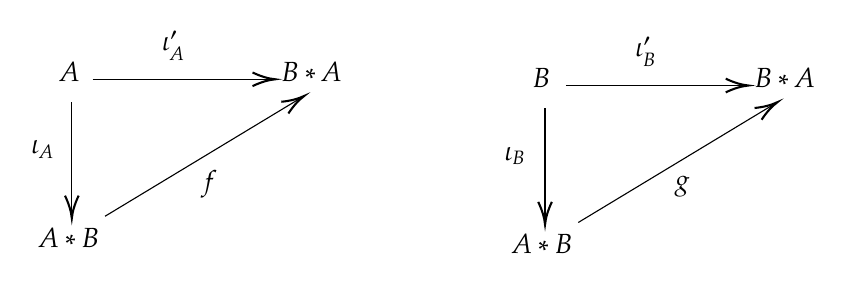
\begin{tikzpicture}[x=0.75pt,y=0.75pt,yscale=-1,xscale=1]
%uncomment if require: \path (0,476); %set diagram left start at 0, and has height of 476

%Straight Lines [id:da51308687576244] 
\draw    (128,112) -- (214,112) ;
\draw [shift={(216,112)}, rotate = 180] [color={rgb, 255:red, 0; green, 0; blue, 0 }  ][line width=0.75]    (10.93,-3.29) .. controls (6.95,-1.4) and (3.31,-0.3) .. (0,0) .. controls (3.31,0.3) and (6.95,1.4) .. (10.93,3.29)   ;
%Straight Lines [id:da945734561567223] 
\draw    (118,123) -- (118,177) ;
\draw [shift={(118,179)}, rotate = 270] [color={rgb, 255:red, 0; green, 0; blue, 0 }  ][line width=0.75]    (10.93,-3.29) .. controls (6.95,-1.4) and (3.31,-0.3) .. (0,0) .. controls (3.31,0.3) and (6.95,1.4) .. (10.93,3.29)   ;
%Straight Lines [id:da6039140489558597] 
\draw    (134,178) -- (228.29,121.03) ;
\draw [shift={(230,120)}, rotate = 148.86] [color={rgb, 255:red, 0; green, 0; blue, 0 }  ][line width=0.75]    (10.93,-3.29) .. controls (6.95,-1.4) and (3.31,-0.3) .. (0,0) .. controls (3.31,0.3) and (6.95,1.4) .. (10.93,3.29)   ;
%Straight Lines [id:da8764595834730253] 
\draw    (356,115) -- (442,115) ;
\draw [shift={(444,115)}, rotate = 180] [color={rgb, 255:red, 0; green, 0; blue, 0 }  ][line width=0.75]    (10.93,-3.29) .. controls (6.95,-1.4) and (3.31,-0.3) .. (0,0) .. controls (3.31,0.3) and (6.95,1.4) .. (10.93,3.29)   ;
%Straight Lines [id:da5299342468146768] 
\draw    (346,126) -- (346,180) ;
\draw [shift={(346,182)}, rotate = 270] [color={rgb, 255:red, 0; green, 0; blue, 0 }  ][line width=0.75]    (10.93,-3.29) .. controls (6.95,-1.4) and (3.31,-0.3) .. (0,0) .. controls (3.31,0.3) and (6.95,1.4) .. (10.93,3.29)   ;
%Straight Lines [id:da1921306060851975] 
\draw    (362,181) -- (456.29,124.03) ;
\draw [shift={(458,123)}, rotate = 148.86] [color={rgb, 255:red, 0; green, 0; blue, 0 }  ][line width=0.75]    (10.93,-3.29) .. controls (6.95,-1.4) and (3.31,-0.3) .. (0,0) .. controls (3.31,0.3) and (6.95,1.4) .. (10.93,3.29)   ;

% Text Node
\draw (111,102.4) node [anchor=north west][inner sep=0.75pt]    {$A$};
% Text Node
\draw (101,182.4) node [anchor=north west][inner sep=0.75pt]    {$A*B$};
% Text Node
\draw (218,102.4) node [anchor=north west][inner sep=0.75pt]    {$B*A$};
% Text Node
\draw (97,140.4) node [anchor=north west][inner sep=0.75pt]    {$\iota _{A}$};
% Text Node
\draw (160,87.4) node [anchor=north west][inner sep=0.75pt]    {$\iota _{A}^{\prime }$};
% Text Node
\draw (179,154.4) node [anchor=north west][inner sep=0.75pt]    {$f$};
% Text Node
\draw (339,105.4) node [anchor=north west][inner sep=0.75pt]    {$B$};
% Text Node
\draw (329,185.4) node [anchor=north west][inner sep=0.75pt]    {$A*B$};
% Text Node
\draw (446,105.4) node [anchor=north west][inner sep=0.75pt]    {$B*A$};
% Text Node
\draw (325,143.4) node [anchor=north west][inner sep=0.75pt]    {$\iota _{B}$};
% Text Node
\draw (388,90.4) node [anchor=north west][inner sep=0.75pt]    {$\iota _{B}^{\prime }$};
% Text Node
\draw (407,157.4) node [anchor=north west][inner sep=0.75pt]    {$g$};


\end{tikzpicture}
\end{center}
here $\iota$ are canonical injections. Then we know that 
$$
\begin{cases}
	\iota _A=g\circ \iota _{A}^{\prime},\\
	\iota _B=g\circ \iota _{B}^{\prime},\\
\end{cases}\hspace{1em}\begin{cases}
	\iota _{A}^{\prime}=f\circ \iota _A,\\
	\iota _{B}^{\prime}=f\circ \iota _B,\\
\end{cases}
$$
hence
$$
\begin{cases}
	\iota _A=\left( g\circ f \right) \circ \iota _A,\\
	\iota _B=\left( g\circ f \right) \circ \iota _B,\\
\end{cases}
$$
therefore $g\circ f=1_{A*B}$. Note that the diagram below is also commutative: 
\begin{center}


\tikzset{every picture/.style={line width=0.75pt}} %set default line width to 0.75pt        

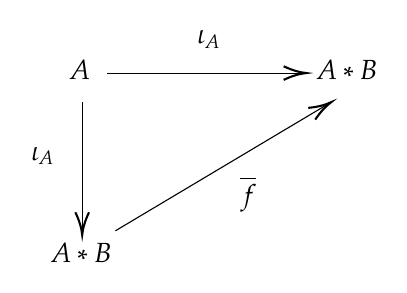
\begin{tikzpicture}[x=0.75pt,y=0.75pt,yscale=-1,xscale=1]
%uncomment if require: \path (0,476); %set diagram left start at 0, and has height of 476

%Straight Lines [id:da1882925271714635] 
\draw    (204,106) -- (298,106) ;
\draw [shift={(300,106)}, rotate = 180] [color={rgb, 255:red, 0; green, 0; blue, 0 }  ][line width=0.75]    (10.93,-3.29) .. controls (6.95,-1.4) and (3.31,-0.3) .. (0,0) .. controls (3.31,0.3) and (6.95,1.4) .. (10.93,3.29)   ;
%Straight Lines [id:da2195364554507213] 
\draw    (192,120) -- (192,182) ;
\draw [shift={(192,184)}, rotate = 270] [color={rgb, 255:red, 0; green, 0; blue, 0 }  ][line width=0.75]    (10.93,-3.29) .. controls (6.95,-1.4) and (3.31,-0.3) .. (0,0) .. controls (3.31,0.3) and (6.95,1.4) .. (10.93,3.29)   ;
%Straight Lines [id:da8375339469219252] 
\draw    (208,182) -- (310.28,121.02) ;
\draw [shift={(312,120)}, rotate = 149.2] [color={rgb, 255:red, 0; green, 0; blue, 0 }  ][line width=0.75]    (10.93,-3.29) .. controls (6.95,-1.4) and (3.31,-0.3) .. (0,0) .. controls (3.31,0.3) and (6.95,1.4) .. (10.93,3.29)   ;

% Text Node
\draw (185,98.4) node [anchor=north west][inner sep=0.75pt]    {$A$};
% Text Node
\draw (176,186.4) node [anchor=north west][inner sep=0.75pt]    {$A*B$};
% Text Node
\draw (304,98.4) node [anchor=north west][inner sep=0.75pt]    {$A*B$};
% Text Node
\draw (166,140.4) node [anchor=north west][inner sep=0.75pt]    {$\iota _{A}$};
% Text Node
\draw (246,84.4) node [anchor=north west][inner sep=0.75pt]    {$\iota _{A}$};
% Text Node
\draw (267,154.4) node [anchor=north west][inner sep=0.75pt]    {$\overline{f}$};


\end{tikzpicture}
\end{center}
hence by the uniqueness of $\overline{f}$ we know that $\overline{f}=1_{A*B}$. Similarly we may show that $\overline{g}=1_{B*A}$. Now consider the commutative diagram below: 
\begin{center}


\tikzset{every picture/.style={line width=0.75pt}} %set default line width to 0.75pt        

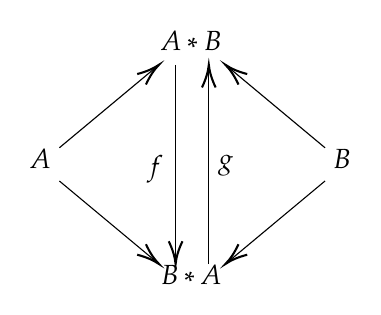
\begin{tikzpicture}[x=0.75pt,y=0.75pt,yscale=-1,xscale=1]
%uncomment if require: \path (0,476); %set diagram left start at 0, and has height of 476

%Straight Lines [id:da19202606498126973] 
\draw    (176,184) -- (222.46,145.28) ;
\draw [shift={(224,144)}, rotate = 140.19] [color={rgb, 255:red, 0; green, 0; blue, 0 }  ][line width=0.75]    (10.93,-3.29) .. controls (6.95,-1.4) and (3.31,-0.3) .. (0,0) .. controls (3.31,0.3) and (6.95,1.4) .. (10.93,3.29)   ;
%Straight Lines [id:da9962758023179532] 
\draw    (176,200) -- (222.46,238.72) ;
\draw [shift={(224,240)}, rotate = 219.81] [color={rgb, 255:red, 0; green, 0; blue, 0 }  ][line width=0.75]    (10.93,-3.29) .. controls (6.95,-1.4) and (3.31,-0.3) .. (0,0) .. controls (3.31,0.3) and (6.95,1.4) .. (10.93,3.29)   ;
%Straight Lines [id:da22458634941235944] 
\draw    (304,184) -- (257.54,145.28) ;
\draw [shift={(256,144)}, rotate = 39.81] [color={rgb, 255:red, 0; green, 0; blue, 0 }  ][line width=0.75]    (10.93,-3.29) .. controls (6.95,-1.4) and (3.31,-0.3) .. (0,0) .. controls (3.31,0.3) and (6.95,1.4) .. (10.93,3.29)   ;
%Straight Lines [id:da6914952904257381] 
\draw    (304,200) -- (257.54,238.72) ;
\draw [shift={(256,240)}, rotate = 320.19] [color={rgb, 255:red, 0; green, 0; blue, 0 }  ][line width=0.75]    (10.93,-3.29) .. controls (6.95,-1.4) and (3.31,-0.3) .. (0,0) .. controls (3.31,0.3) and (6.95,1.4) .. (10.93,3.29)   ;
%Straight Lines [id:da6281527000369735] 
\draw    (232,144) -- (232,238) ;
\draw [shift={(232,240)}, rotate = 270] [color={rgb, 255:red, 0; green, 0; blue, 0 }  ][line width=0.75]    (10.93,-3.29) .. controls (6.95,-1.4) and (3.31,-0.3) .. (0,0) .. controls (3.31,0.3) and (6.95,1.4) .. (10.93,3.29)   ;
%Straight Lines [id:da04897854339512486] 
\draw    (248,240) -- (248,146) ;
\draw [shift={(248,144)}, rotate = 90] [color={rgb, 255:red, 0; green, 0; blue, 0 }  ][line width=0.75]    (10.93,-3.29) .. controls (6.95,-1.4) and (3.31,-0.3) .. (0,0) .. controls (3.31,0.3) and (6.95,1.4) .. (10.93,3.29)   ;

% Text Node
\draw (161,183.4) node [anchor=north west][inner sep=0.75pt]    {$A$};
% Text Node
\draw (307,183.4) node [anchor=north west][inner sep=0.75pt]    {$B$};
% Text Node
\draw (224,126.4) node [anchor=north west][inner sep=0.75pt]    {$A*B$};
% Text Node
\draw (224,239.4) node [anchor=north west][inner sep=0.75pt]    {$B*A$};
% Text Node
\draw (217,186.4) node [anchor=north west][inner sep=0.75pt]    {$f$};
% Text Node
\draw (251,186.4) node [anchor=north west][inner sep=0.75pt]    {$g$};


\end{tikzpicture}
\end{center}
By $f\circ g=1_{B*A}$ and $g\circ f=1_{A*B}$ we know that there exists an isomorphism between $A*B$ and $B*A$, hence $A*B\cong B*A$. Similarly we may proof the associativity.
\end{proof}
\begin{problem}\em
If $N$ is the normal subgroup of $A*B$ generated by $A$, then $(A*B)/N\cong B$.
\end{problem}
\begin{proof}
We consider the canonical projection $\pi_A:A*B\to B$. Then it is easy to verify that $\mathrm{Ker}\pi_A=N$. Therefore by the First Isomorphism Theorem we know $(A*B)/N\cong B$.
\end{proof}
\begin{problem}\em
If $G$ and $H$ each have more than one element, then $G*H$ is an infinite group with center $\left<e\right>$.
\end{problem}
\begin{proof}
It is clear that $(ab)^n$, $n\in\mathbb{Z}$ differs since the length of them differs. Hence $G*H$ is infinite. Now we show that $Z(A*B)=\left<e\right>$. Consider $w\in A*B$. Without loss of generality we may assume $W$ ends with $a_r$, which is a word in $A$. Therefore for all $b\in B$, clearly $bw\ne wb$ since $bw$ ends with a word in $A$, but $wb$ ends with a word in $B$. Since this is true for all nontrivial $w\in A*B$, we conclude that $Z(A*B)=\left<e\right>$.
\end{proof}
\begin{problem}\em
A free group is a free product of infinite cyclic groups.
\end{problem}
\begin{proof}
Let $F$ be a free group on $X$. Then $F=\left<X\right>$. Hence $F$ is the free product ${\prod}^*_{x\in X}\left<x\right>$, which is a free product of infinite cyclic groups.
\end{proof}
\newpage
\section{The Structure of Groups}
In this chapter, we continue our study on group theory to get some depth for certain classes of abelian groups and for various classes of groups that share some desirable properties with abelian groups. We shall always use additive notation in this chapter. We give a dictionary of notations: 
$$
\begin{matrix}
	\mathrm{additive}\ \mathrm{notation}&		\mathrm{multiplicative}\ \mathrm{notation}\\
	a+b&		ab\\
	-a&		a^{-1}\\
	0&		e\\
	na&		a^n\\
	a-b&		ab^{-1}\\
	H+K&		HK\\
	a+H&		aH\\
	G\oplus H&		G\times H\\
	H+K&		H\lor K\\
	\sum_{i\in I}{G_i}&		{\prod}^w_{i\in I}{G_i}\\
	\mathrm{direct}\ \mathrm{sum}&		\mathrm{weak}\ \mathrm{direct}\ \mathrm{product}\\
\end{matrix}
$$
\subsection{Free Abelian Groups}
We shall investigate free objects in the category of abelian groups. First we introduce some terminology.\par
Let $G$ be a group of additive notation. If $X$ is a nonempty subset of $G$, then $\left<X\right>$ contains all \textbf{linear combinations} $n_1x_1+n_2x_2+\cdots+n_kx_k(n_i\in\mathbb{Z},x_i\in X)$. In particular, the cyclic group $\left<x\right>=\{nx:n\in\mathbb{Z}\}$.\par
A \textbf{basis} of an abelian group $F$ is a subset $X$ of $F$ such that $F=\left<X\right>$, and for distinct $x_1,x_2,\cdots,x_k\in X$ and $n_i\in\mathbb{Z}$, 
$$n_1x_1+n_2x_2+\cdots+n_kx_k=0\Rightarrow n_i=0\ \text{for every} \ i.$$
\begin{theorem}
The following conditions on an abelian group $F$ are equivalent.\par
(i) $F$ has a nonempty basis.\par
(ii) $F$ is the (internal) direct sum of a family of infinite cyclic subgroups.\par
(iii) $F$ is isomorphic to a direct sum of copies of the additive group $\mathbb{Z}$ of integers.\par
(iv) There exists a nonempty set $X$ and a function $\iota:X\to F$ with the following property: given an abelian group $G$ and function $f:X\to G$, there exists a unique homomorphism of groups $\overline{f}:F\to G$ such that $\overline{f}\iota=f$. In other words, $F$ is free object in the category of abelian groups.
\end{theorem}
We call the abelian group satisfying conditions above a \textbf{free abelian group}. By definition the trivial group $0$ is the free abelian group on the null set $\emptyset$.
\begin{proof}
(i)$\Rightarrow$(ii): Let $X$ be a basis of $F$, we show that $F=\sum_{x\in X}\left<x\right>$, which is the direct sum of infinite cyclic subgroups (if finite, then there exists some $n\in\mathbb{Z}$ such that $nx=0$, which contradict to the fact that $X$ is a basis). Since $F=\left<X\right>$, we know that $F=\left<\bigcup_{x\in X}x\right>$. Let $x_0\in X$, we consider $\left<x_0\right>\cap\left<\bigcup_{x\in X\setminus\{x_0\}}x\right>$. If $\left<x_0\right>\cap\left<\bigcup_{x\in X\setminus\{x_0\}}x\right>\ne 0$, then there exists some $k_0,k_1,\cdots,k_n$ such that $k_0x_0=k_1x_1+k_2x_2+\cdots+k_nx_n\ne 0$, here $x_i\in X,0\le i\le n$. However, since $X$ is a basis we know that $k_0=k_1=\cdots=k_n=0$, which is a contradiction! Hence by the definition of a direct sum we know that $F=\sum_{x\in X}\left<x\right>$.\par
(ii)$\Rightarrow$(iii): Since $\left<x\right>$ are infinite cyclic groups, then $\left<x\right>\cong\mathbb{Z}$. Hence by theorem 2.69 we know that $F=\sum_{x\in X}\left<x\right>\cong\sum_{|X|}\mathbb{Z}$.
\par
(iii)$\Rightarrow$(i): Let $F\cong\sum\mathbb{Z}$, where $\mathbb{Z}$ are indexed with a set $X$. For each $x\in I$, let $\theta_x$ be the element $\{u_i\}\in\sum\mathbb{Z}$ satisfying $u_i=0$ for $i\ne x$ and $u_x=1$. Therefore it is easy to verify $\{\theta_x\}$ is a basis of $\sum\mathbb{Z}$. Then by $F\cong\sum\mathbb{Z}$ we may define a basis of $F$ by isomorphism.\par
(i)$\Rightarrow$(iv): Let $X$ be the basis of $F$ and $\iota:X\to F$ be the inclusion map. Given $G$ abelian and map $f:X\to G$, we define $\overline{f}:F\to G$ by $\sum_{i\in I}n_ix_i\mapsto\sum_{i\in I}n_if(x_i)$. We first show that $\overline{f}$ is well-defined. Let $x\in F$, then $x=\sum_{i\in I}n_ix_i$ for some $n_i$ and $x_i$. Now if $x=\sum_{i\in I}m_ix_i$, then $\sum_{i\in I}(n_i-m_i)x_i=0$, hence $n_i=m_i$ since $X$ is a basis of $F$. It is easy to show that $\overline{f}$ is a homomorphism since $F$ is abelian. Now observed that $\overline{f}\iota \left( x \right) =\overline{f}\left( x \right) =f\left( x \right) $ for all $x\in X$, hence $\overline{f}\iota=f$. If there is another $g$ satisfies $g\iota=f$, then $g\left( x \right) =g\iota \left( x \right) =f\left( x \right) =\overline{f}\iota \left( x \right) =\overline{f}\left( x \right) $, hence $\overline{f}=g$, which proved the uniqueness.\par
(iv)$\Rightarrow$(iii): Let $\iota:X\to F$. We construct a direct sum $\sum\mathbb{Z}$ indexed with $X$. Now take $Y=\{\theta_x\}$ as in the proof of (iii)$\Rightarrow$(i). By (iii)$\Rightarrow$(i)$\Rightarrow$(iv) we know that $\sum\mathbb{Z}$ is a free object on $Y$. It is trivial that $|X|=|Y|$, hence by theorem 2.59 we know that $F\cong\sum\mathbb{Z}$, hence $F$ has a nonempty basis.
\end{proof}
Theorem 3.1 indicates how to construct a free abelian group $F$ with basis $X$. Simply let $F$ be the direct sum $\sum\mathbb{Z}$, with the copies of $\mathbb{Z}$ indexed by $X$. As in the proof (iii)$\Rightarrow$(i), $\{\theta_x:x\in X\}$ is a basis of $F=\sum\mathbb{Z}$, and $F$ is free on the set $\{\theta_x:x\in X\}$. Since the map $\iota:X\to F$ is injective, it follows easily that $F$ is free on $X$ in the sense of (iv). In this situation we shall identify $X$ with its image under $\iota$ so that $X\subset F$ and the cyclic group $\left<\theta_x\right>=\{n\theta_x:n\in\mathbb{Z}\}=\mathbb{Z}\theta_x$ is written $\left<x\right>=\mathbb{Z}x$. In this notation $F=\sum_{x\in X}\left<\theta_x\right>=\sum_{x\in X}\mathbb{Z}x$, and a typical element of $F$ has the form $n_1x_1+n_2x_2+\cdots+n_kx_k(n_i\in\mathbb{Z},x_i\in X)$. In particular, $X=\iota(X)$ is a basis of $F$.
\begin{theorem}
Any two bases of a free abelian group $F$ have the same cardinality.
\end{theorem}
\begin{proof}
First suppose $F$ has a basis $X$ of finite cardinality $n$ so that $F\cong\mathbb{Z}\oplus\mathbb{Z}\oplus\cdots\oplus\mathbb{Z}$ ($n$ summands). For any subgroup $G$ of $F$, it is easy to verify that $2G$ is a subgroup of $G$. Hence we may restrict the isomorphism $F=\mathbb{Z}\oplus\mathbb{Z}\oplus\cdots\oplus\mathbb{Z}$ to $2F$, which is $2F\cong2\mathbb{Z}\oplus2\mathbb{Z}\oplus\cdots\oplus2\mathbb{Z}$. Hence by corollary 2.70 we have $F/2F\cong\mathbb{Z}/2\mathbb{Z}\oplus\mathbb{Z}/2\mathbb{Z}\oplus\cdots\oplus\mathbb{Z}/2\mathbb{Z}$. Therefore $|F/2F|=2^n$. Let $Y$ be another basis of $F$. Then by the same argument we may show that $|F/2F|=2^{|Y|}$, hence $|Y|=|X|=n$.\par
Now we suppose one of the basis of $F$ is infinite. Then all the bases of $F$ is infinite by the previous paragraph. Now we show that $|X|=|F|$. It is trivial that $|X|\le |F|$. Conversely, let $S=\bigcup_{n\in\mathbb{N}_+}X^n$, where $X^n=X\times X\times\cdots\times X$ ($n$ factors). Then for each $s=(x_1,x_2,\cdots,x_s)\in S$ let $G_s$ be the subgroup $\left<x_1,x_2,\cdots,x_n\right>$. Then $G_s\cong\mathbb{Z}y_1\oplus\cdots\oplus\mathbb{Z}y_k$, where $y_1,\cdots,y_k$ are distinct elements of $x_1,x_2,\cdots,x_n$. Therefore $|G_s|=|\mathbb{Z}^t|=|\mathbb{Z}|=\aleph_0$ by the knowledge of cardinal numbers. Since $F=\bigcup_{s\in S}G_s$, we have $|F|=\left|\bigcup_{s\in S}G_s\right|\le|S|\aleph_0$. Therefore $|S|=|X|$, whence $|F|\le|X|\aleph_0=|X|$. Therefore by Cantor-Bernstein Theorem we have $|X|=|F|$, which finished our proof.
\end{proof}
\begin{note}\em
The cardinal number of any basis $X$ of the free abelian group $F$ is called the \textbf{rank} of $F$.
\end{note}
By theorem 3.2 we immediate get the proposition below:
\begin{proposition}
Let $F_1$ be the free abelian group on the set $X_1$ and $F_2$ be the free abelian group on the set $X_2$. Then $F_1\cong F_2$ if and only if $F_1$ and $F_2$ have the same rank, that is, $|X_1|=|X_2|$.
\end{proposition}
\begin{proof}
If $F_1\cong F_2$, let $\alpha:F_1\to F_2$ be an isomorphism. Then $\alpha(X_1)$ is a basis of $F_2$, whence $|X_1|=|\alpha(X_1)|=|X_2|$ by theorem 3.2, hence $F_1$ and $F_2$ have the same rank.
\end{proof}
\begin{theorem}
Every abelian group $G$ is the homomorphic image of a free abelian group of rank $|X|$, where $X$ is set of generators of $G$.
\end{theorem}
\begin{proof}
Let $F$ be the free abelian group on the set $X$. Then $F=\sum_{x\in X}\mathbb{Z}x$ and rank $F=|X|$. By theorem 3.1 the inclusion map $X\to G$ induces a homomorphism $\overline{f}:F\to G$ such that $1x\mapsto x$. Hence $X\subset\mathrm{Im}\overline{f}\subset G$. Since $X$ generates the whole $G$, we have $\mathrm{Im}\overline{f}=G$.
\end{proof}
We now proof a theorem that will be extremely useful in analyzing the structure of finitely generated groups. We shall need 
\begin{lemma}\em
If $\{x_1,x_2,\cdots,x_n\}$ is a basis of a free abelian group $F$ and $a\in\mathbb{Z}$, then for all $i\ne j$ $\{x_1,\cdots,x_{j-1},x_j+ax_i,x_{j+1},\cdots,x_n\}$ is also a basis of $F$.
\end{lemma}
\begin{proof}
First observed that $x_j=-ax_i+(x_j+ax_i)$, hence $F=\left<x_1,\cdots,x_{j-1},x_j+ax_i,x_{j+1},\cdots,x_n\right>$. Now it suffices to show that $\{x_1,\cdots,x_{j-1},x_j+ax_i,x_{j+1},\cdots,x_n\}$ is a basis. Let
$$
k_1x_1+\cdots +k_{j-1}x_{j-1}+k_j\left( x_j+ax_i \right) +k_{j+1}x_{j+1}+\cdots +k_nx_n=0,
$$
since $\{x_1,x_2,\cdots,x_n\}$ is a basis we know that $k_i=0,i=1,2,\cdots,n$.
\end{proof}
\begin{theorem}
If $F$ is a free abelian group of finite rank $n$ and $G$ is a nonzero subgroup of $F$, then there exists a basis $\{x_1,x_2,\cdots,x_n\}$ of $F$, an integer $r(1\le r\le n)$ and positive integers $d_1,d_2,\cdots,d_r$ such that $d_1\mid d_2\mid\cdots\mid d_r$ and $G$ is free abelian with basis $\{d_1x_1,d_2x_2,\cdots,d_rx_r\}$. 
\end{theorem}
\begin{proof}
We proof by induction. If $n=1$, then $F=\left<x_1\right>\cong\mathbb{Z},G=\left<d_1x_1\right>\cong\mathbb{Z}$. Now we assume the statement is true for all $F$ whose rank is less than $n$. Let $S$ be a set and $s\in S$ if and only if there exists a basis $\{y_1,y_2,\cdots,y_n\}$ of $F$ and an element in $G$ of the form $sy_1+k_2y_2+\cdots+k_ny_n,k_i\in\mathbb{Z}$. Note that in this case $\{y_2,y_1,\cdots,y_n\}$ is also a basis of $F$ and hence $k_2\in S$. Similarly $k_i\in S$ for all $i=2,3,\cdots,n$. Note that $S$ is nonempty, hence we may select an integer $d_1\in S$ that is the least number in $S$. Therefore for some basis $\{y_1,y_2,\cdots,y_n\}$ there exists $v=d_1x_1+k_2x_2+\cdots+k_nx_n$. By the division algorithm for each $i=2,3,\cdots,n$ we have $k_i=q_id_1+r_i$, here $0\le r_i<d_1$. Hence $v=d_1\left( y_1+q_2y_2+\cdots +q_ny_n \right) +r_2y_2+\cdots +r_ny_n$. Now define $x_1=y_1+q_2y_2+\cdots +q_ny_n$, then by lemma 3.1 we know that $\{x_1,y_2,\cdots,y_n\}$ is also a basis of $F$. Since $v\in G$ we know by the minimum of $d_1$ that $r_i=0$ for all $i=2,3,\cdots,n$. Therefore $v=d_1x_1\in G$.\par
Now let $H=\left<x_2,x_3,\cdots,x_n\right>$. Trivially $F=\left<x_1\right>\oplus H$. Furthermore we claim that $G=\left<v\right>\oplus(G\cap H)=\left<d_1x_1\right>\oplus(G\cap H)$. It is clear that $\left<d_1x_1\right>\cap(G\cap H)=0$. It suffices to show that $G=\left< v \right> +\left( G\cap H \right) $. Let $u=t_1x_1+t_2y_2+\cdots+t_ny_n\in G$, then by division algorithm $t_i=d_iq_i+r_i$ for all $i=2,3,\cdots,n$. Thus $G$ contains $u-q_1v=r_1x_1+t_2x_2+\cdots+t_nx_n$. Then by the minimal property of $d_1$ we have $r_1=0$. Hence $u-q_1v\in H$, therefore $u\in q_v+H$, which is $G=\left<d_1x_1\right>+H$, which proved our assertion.\par
Now if $G\cap H=0$, the proof has been finished. So we discuss the condition $G\cap H\ne 0$. Then by the inductive assumption we have a basis $\{x_2,x_3,\cdots,x_n\}$ and an integer $r\le n$ and $d_2,d_3,\cdots,d_r$, such that $d_2\mid d_3\mid\cdots\mid d_r$ and $G\cap H$ is free abelian we basis $\{D_2x_2,d_3x_3,\cdots,d_rx_r\}$. Since $F=\left<x_1\right>\oplus H$ and $G=\left<d_1x_1\right>\oplus(G\cap H)$, it follows that $\{x_1,x_2,\cdots,x_n\}$ is a basis of $F$ and $\{d_1x_1,d_2x_2,\cdots,d_rx_r\}$ is a basis of $G$. Now it suffices to show that $d_1\mid d_2$. By the division algorithm let $d_2=qd_1+r_0$ with $0\le r_0<d_1$. Since $\{x_2,x_1+qx_2,x_3,\cdots,x_n\}$ is a basis of $F$ by lemma 1.1 and $r_0x_2+d_1(x_1+qx_2)=d_1x_1+d_2x_2\in G$, the minimal property of $d_1$ implies $r_0=0$, whence $d_1\mid d_2$.
\end{proof}
\begin{corollary}
If $G$ is a finitely generated abelian group generated by $n$ elements, then every subgroup $H$ of $G$ may be generated by $m$ elements with $m\le n$.
\end{corollary}
\begin{proof}
By theorem 1.4 we know that there exists an epimorphism $\pi:F\to G$. Consider $\pi^{-1}(H)$, which is a subgroup of $F$ and by theorem 1.5 we know that the rank of $\pi^{-1}(H)$ is less than $n$. The image under $\pi$ of a basis of $\pi^{-1}(H)$ is a basis that generates $\pi(\pi^{-1}(H))=H$ and hence the rank $m$ of $H$ satisfies $m\le n$.
\end{proof}
\begin{center}
\begin{large}
    \textbf{Exercises for 3.1}
\end{large}
\end{center}
\begin{problem}\em
(a) If $G$ is an abelian group and $m\in\mathbb{Z}$, then $mG=\{mg:g\in G\}$ is the subgroup of $G$.\par
(b) If $G\cong\sum_{i\in I}G_i$, then $mG\cong\sum_{i\in I}mG_i$ and $G/mG\cong\sum_{i\in I}G_i/mG_i$.
\end{problem}
\begin{proof}
(a) We proof by definition. Clearly $mG$ is associative. Since $0\in G$, we have $m0=0\in mG$, hence $mG$ has identity element. Also for $mg\in mG$ we have $m(-g)=-mg$ be the inverse of $mg$, hence $mG$ is a group. Trivially $mG\subset G$, hence $mG$ is the subgroup of $G$.\par
(b) Let $g\in G$. Since $G\cong\sum_{i\in I}G_i$ we may write $g=\sum_{i\in I}g_i$, where $g_i\in G_i$. Hence $mg=m\sum_{i\in I}g_i=\sum_{i\in I}mg_i$, therefore $mG\cong\sum_{i\in I}mG_i$. Then by corollary 2.70 we have $G/mG\cong\left(\sum_{i\in I}G_i\right)/\left(\sum_{i\in I}mG_i\right)\cong\sum_{i\in I}G_i/mG_i$.
\end{proof}
\begin{problem}\em
A subset $X$ of an abelian group $F$ is said to be \textbf{linearly independent} if $n_1x_1+n_2x_2+\cdots+n_kx_k=0$ always implies $n_i=0$ for all $i$, where $n_i\in\mathbb{Z}$ and $x_i$ be distinct elements of $X$.\par
(a) $X$ is linearly independent if and only if every nonzero element of the subgroup $\left<X\right>$ may be written uniquely in the form $n_1x_1+n_2x_2+\cdots+n_kx_k$.\par
(b) If $F$ is free abelian of finite rank $n$, it it not true that every linearly independent subset of $n$ element is a basis.\par
(c) If $F$ is free abelian, it is not true that every linearly independent subset of $F$ may be extended to a basis of $F$.\par
(d) If $F$ is free abelian, it is not true that every generating set of $F$ contains a basis of $F$. However, if $F$ is also finitely generated by $n$ elements, then $F$ has a rank $m\le n$.
\end{problem}
\begin{proof}
(a) By theorem 2.14 we know that for all $x\in\left<X\right>$ it has the form $x=a_1x_1+a_2x_2+\cdots+a_kx_k$. Now we proof the uniqueness. Let $x=b_1x_1+b_2x_2+\cdots+b_kx_k$, then $\sum_{i=1}^k(a_i-b_i)x_i=0$. Since $X$ is linearly independent we have $a_i=b_i$ for all $i$, whence we finished our proof.\par
(b) and (c) Consider $\mathbb{Z}$ and subset $\{2\}$.\par
(d) Consider $\mathbb{Z}$ and subset $\{2,3\}$. Now we show that if $F$ can be generated by a set $X$ with $n$ elements, then the rank of $F$ must be less than $n$. Let $F=\left<X\right>$. If $X$ is a basis of $F$, then the rank of $F$ is $n$. Otherwise there exists some integers $k_1,k_2,\cdots,k_n$ such that $k_1x_1+k_2x_2+\cdots+k_nx_n=0$, but there exists $k_i\ne 0$. Suppose $k_ix_i=\sum k_j^\prime x_j$, then by lemma 3.1 we know $X\setminus\{x_i\}$ also generates the whole $F$. Hence the rank of $F$ is less than $n$.
\end{proof}
\begin{problem}\em
Let $X=\{a_i:i\in I\}$ be a set. Then the free abelian group on $X$ is isomorphic to the group defined by the generators $X$ and the relations $\{a_ia_ja_i^{-1}a_j^{-1}=e:a_i,a_j\in X\}$.
\end{problem}
\begin{proof}
By the relation we know that elements in $\left<X\right>$ are commutative. Now we show that $\left<X\right>$ is free. Since elements of $\left<X\right>$ has the form (we use the additive notation) $x=\sum_{i\in I}k_ia_i$, here $k_i\in\mathbb{Z}$ and $i\in I$. Therefore $\left<X\right>=\sum_{i\in I}\mathbb{Z}a_i$, which can be written as the direct sum of a family of cyclic groups, hence $\left<X\right>$ is a free abelian group.
\end{proof}
\begin{problem}\em
A free abelian group is a free group if and only if it is cyclic.
\end{problem}
\begin{proof}
If a free abelian group is free, then it must be generated by one element (otherwise does not commute, hence not abelian. Consider $abab\cdots$), therefore cyclic. Conversely, if a free abelian group if cyclic, then for a map $f:X\to F$, here $X$ is a basis of $F$, let $\overline{f}:F\to G$ be $a^n\mapsto f^n(a)$, therefore $\overline{f}$ is a homomorphism and $\overline{f}\iota=f$, where $\iota:X\to F$ is the canonical injection. Therefore $F$ is free on $X$.
\end{proof}
\begin{problem}\em
The direct sum of a family of free abelian groups is a free group.
\end{problem}
\begin{proof}
Let $\{G_i:i\in I\}$ be a class of free abelian groups. Then $G_i=\sum_{k}G_{ik}$ for all $i\in I$, where $G_{ik}$ are cyclic groups. Therefore $G=\sum_{i\in I}G_i=\sum_{i\in I}\sum_{k}G_{ik}$ is the sum of some cyclic groups, and hence free abelian.
\end{proof}
\begin{note}\em
A direct product of free abelian groups need not to be abelian. See L. Fuchs \textit{Infinite Abelian Groups}.
\end{note}
\begin{problem}\em
If $F=\sum_{x\in X}\mathbb{Z}x$ is a free abelian group, and $G$ is the subgroup with basis $X^\prime=X\setminus\{x_0\}$ for some $x_0\in X$, then $F/G\cong\mathbb{Z}x_0$. Generalize this result to arbitrary subsets $X^\prime$ of $X$.
\end{problem}
\begin{proof}
We define the canonical injection $\pi_0:F\to\mathbb{Z}x_0$ by $\sum_{x\in X}k_xx\mapsto k_{x_0}x_0$. Therefore $\mathrm{Ker}\pi_0=G$, hence by the First Isomorphism Theorem we have $F/\mathrm{Ker}\pi_0=F/G\cong\mathbb{Z}x_0$. For an arbitrarily chosen $X^\prime\subset X$, let $G$ be the group with basis $X^\prime$, similarly we have $F/G\cong\sum_{x\in X\setminus X^\prime}\mathbb{Z}x$.
\end{proof}
\begin{problem}\em
A nonzero free abelian group has a subgroup of index $n$ for every positive integer $n$.
\end{problem}
\begin{proof}
It suffices to show that for all integer $n$ there exists an injection $\mathbb{Z}/n\mathbb{Z}\to\mathbb{Z}$, which can be defined by $\overline{k}\mapsto k$, by which we finished our proof.
\end{proof}
\begin{problem}\em
Let $G$ be a finitely generated abelian group in which no element has finite order except $0$. Show that $G$ is free abelian.
\end{problem}
\begin{proof}
Let $\{x_1,x_2,\cdots,x_n\}$ be the set of all generators of $G$. Then we define $f:\mathbb{Z}^n\to G$ by $(a_1,a_2,\cdots,a_n)\mapsto a_1x_1+a_2x_2+\cdots+a_nx_n$, which is an epimorphism. Since $\mathrm{Ker}f<\mathbb{Z}^n$, where $\mathbb{Z}^n$ is free abelian with basis $\{y_1,y_2,\cdots,y_n\}$, hence by theorem 3.5 we know that there exists an integer $0\le r\le n$ and $d_1\mid d_2\mid\cdots\mid d_r$, such that $\mathrm{Ker}f$ is generated by $\{d_1y_1,d_2y_2,\cdots,d_ry_r\}$. Hence $\mathrm{Ker}f=\mathbb{Z} d_1y_1\oplus \mathbb{Z} d_2y_2\oplus \cdots \oplus \mathbb{Z} d_ry_r.$
Therefore 
$$
\mathbb{Z} ^n/\mathrm{Ker}f\cong \left( \mathbb{Z} y_1\oplus \mathbb{Z} y_2\oplus \cdots \oplus \mathbb{Z} y_n \right) /\left( \mathbb{Z} d_1y_1\oplus \mathbb{Z} d_2y_2\oplus \cdots \oplus \mathbb{Z} d_ry_r \right) \cong \left( \sum_{i=1}^r{\mathbb{Z} /\mathbb{Z} d_i} \right) \oplus \mathbb{Z} ^{n-r},
$$
which forces $r=0$, otherwise there exists some elements of finite order since $\mathbb{Z}/\mathbb{Z}d_i$ is finite cyclic. Hence $G\cong\mathbb{Z}^n$ and we finished our proof.
\end{proof}
\begin{note}\em
We call a group with all of its elements infinite order a \textbf{torsion-free group}. Conversely, a group with all of its elements finite order is a \textbf{torsion group}. There exists a group that is neither torsion group nor torsion-free group. 
\end{note}
\begin{problem}\em
(a) Show that the additive group of rationals $\mathbb{Q}$ is not free generated.\par
(b) Show that $\mathbb{Q}$ is not free.\par
(c) Conclude that exercise 3.8 is false if the hypothesis "finitely generated" is omitted.
\end{problem}
\begin{proof}
(a) Suppose $\mathbb{Q}$ is finitely generated, then there exists $d_1\mid d_2\mid\cdots\mid d_r$ such that 
$$
\mathbb{Q} \cong \mathbb{Z} /d_1\mathbb{Z} \oplus \mathbb{Z} /d_2\mathbb{Z} \oplus \cdots \oplus \mathbb{Z} /d_r\mathbb{Z} \oplus \mathbb{Z} ^m.
$$
If $r\ge 1$, then there exists some $x\in\mathbb{Q}$ such that $d_ix=0$ and $x\ne 0$, which is a contradiction! Hence $r=0$ and $\mathbb{Q}\cong\mathbb{Z}^m$. Therefore there exists some $x_1,x_2\in\mathbb{Q}$ such that $x_1$ and $x_2$ are linearly independent over $\mathbb{Z}$. However, let $x_i=\frac{a_i}{b_i}(i=1,2)$, then $a_2b_1x_1-a_1b_2x_2=0$, contradiction! Hence $\mathbb{Q}\cong\mathbb{Z}$, and hence cyclic. However, suppose $\mathbb{Q}$ is generated by $\frac{a}{b}$, consider $\frac{1}{b+1}$ (or $\frac{1}{b+2}$ if $b=-1$), which can not be generated by $\frac{a}{b}$, again a contradiction! Hence $\mathbb{Q}$ is not finitely generated.\par
(b) If $\mathbb{Q}$ is free, then $\mathbb{Q}\cong\sum_{I}\mathbb{Z}$, which has been shown to be impossible in (a).\par
(c) Consider $\mathbb{Q}$, it is abelian, but not finite generated. Also it is not free.
\end{proof}
\begin{problem}\em
(a) Let $G$ be the additive group of all polynomials in $x$ with integer coefficients. Show that $G$ is isomorphic to the group $\mathbb{Q}^*$ of all positive rationals (under multiplication).\par
(b) The group $\mathbb{Q}^*$ is free abelian with basis $\{p:\text{$p$ is prime in $\mathbb{Z}$}\}$.
\end{problem}
\begin{proof}
(a) We define the map $f:G\to\mathbb{Q}^*$ by $\sum_{k=0}^n{a_kx^k}\mapsto \prod_{k=0}^n{p_{k}^{a_k}}$, where $p_k$ is the $\{p_n\}_{n=0}^\infty$ are permutations of all prime numbers. First $f$ is homomorphism since 
$$
\sum_{k=0}^n{a_kx^k}+\sum_{k=0}^n{b_kx^k}=\sum_{k=0}^n{\left( a_k+b_k \right) x^k}\mapsto \prod_{k=0}^n{p_{k}^{a_k+b_k}}=\prod_{k=0}^n{p_{k}^{a_k}}\cdot \prod_{k=0}^n{p_{k}^{b_k}}.
$$
By the Fundamental Theorem of Arithmetic we know that it is an isomorphism, and hence $G\cong\mathbb{Q}^*$.\par
(b) By (a) it suffices to show that $G$ is free abelian, which is given by the fact that $G\cong\sum_{n\in \mathbb{N} _+}{\mathbb{Z} x^n}$.
\end{proof}
\subsection{Finitely Generated Abelian Groups}
We begin by proving two different structure theorems for finitely generated abelian groups. A uniqueness theorem then shows that each structure theorem provides a set of numerical invariants for a given group. From this section on we write $\bigoplus$ for direct sums and $\sum$ for sums of elements.\par
All the theorems here are special cases of corresponding theorems for finitely generated modules over a principal ideal domain, which will be discussed in chapter 5. Some readers may prefer the method of proof used in chapter 5 to the one used here, which depends heavily in Theorem 3.5.\par
Note that most of the theorems in this section may be extended to certain abelian groups that are not finitely generated, readers that are interested in may refer to \textit{Infinite Abelian Groups} by L.Fuchs or \textit{Infinite Abelian Groups} by I.Kaplansky (The name of two books are the same but of different authors).
\begin{theorem}
Every finitely generated abelian group $G$ is isomorphic to a finite direct sum of cyclic groups in which the finite cyclic groups summands (if any) are of orders $m_1,m_2,\cdots,m_n$, where $m_1>1$ and $m_1\mid m_2\mid\cdots\mid m_t$.
\end{theorem}
\begin{proof}
By theorem 3.4 we know that there exists a free abelian group $F$ and an epimorphism $\pi:F\to G$. If $\pi$ is an isomorphism, then $F\cong G\cong\mathbb{Z}\oplus\mathbb{Z}\oplus\cdots\oplus\mathbb{Z}$. Otherwise consider $\mathrm{Ker}\pi$, which is the subgroup of $F$ and hence by theorem 3.5 there exists $d_1,d_2,\cdots,d_r$ such that $d_1\mid d_2\mid\cdots\mid d_r$ and $\mathrm{Ker}\pi=\bigoplus_{i=1}^r\left<d_ix_i\right>$. Now $F=\bigoplus_{i=1}^n\left<x_i\right>\cong\bigoplus_{i=1}^n\mathbb{Z}$ and $\mathrm{Ker}\pi=\bigoplus_{i=1}^n\left<d_ix_i\right>\cong\bigoplus_{i=1}^nd_i\mathbb{Z}$ if we define $d_i=0$ for $i>r$. Therefore by the First Isomorphism Theorem we have 
$$
G\cong F/\mathrm{Ker}\pi =\left( \bigoplus_{i=1}^n{\left< x_i \right>} \right) {/}\left( \bigoplus_{i=1}^n{\left< d_ix_i \right>} \right) \cong \bigoplus_{i=1}^n{\left< x_i \right> /\left< d_ix_i \right>}\cong \bigoplus_{i=1}^n{\mathbb{Z} /d_i\mathbb{Z}},
$$
which is $G\cong\mathbb{Z}_{d_1}\oplus\mathbb{Z}_{d_2}\oplus\cdots\oplus\mathbb{Z}_{d_r}\oplus\mathbb{Z}\oplus\cdots\oplus\mathbb{Z}$, where $\mathbb{Z}\oplus\cdots\oplus\mathbb{Z}$ has rank $s$, $s=n-r$.
\end{proof}
\begin{theorem}
Every finitely generated abelian group $G$ is isomorphic to a finite direct sum of cyclic groups, each of which is either infinite or of order a power of a prime.
\end{theorem}
To prove this theorem, we need the lemma below:
\begin{lemma}\em
If $m$ is a positive integer and $m=p_1^{a_1}p_2^{a_2}\cdots p_k^{a_k}$, then 
$$\mathbb{Z}_m\cong\mathbb{Z}_{p_1^{a_1}}\oplus\mathbb{Z}_{p_2^{a_2}}\oplus\cdots\oplus\mathbb{Z}_{p_k^{a_k}}.$$
\end{lemma}
\begin{proof}
We prove by induction. It suffices to show that $\mathbb{Z}_{rn}=\mathbb{Z}\oplus\mathbb{Z}_n$ when $(r,n)=1$. The element $n=n1\in\mathbb{Z}_{rn}$ has order $r$, whence $\mathbb{Z}_r\cong\left<n1\right><\mathbb{Z}_{rn}$ and the map $\psi_1:\mathbb{Z}_r\to\mathbb{Z}_{rn}$ given by $k\mapsto nk$ is a monomorphism. Similarly the map $\psi_2:\mathbb{Z}_n\to\mathbb{Z}_{rn}$ is a monomorphism. Now we define $\psi:\mathbb{Z}_r\oplus\mathbb{Z}_n\mapsto\mathbb{Z}_{rn}$ by $(x,y)\mapsto\psi_1(x)+\psi_2(y)$, which is easy to show that to be well-defined. Since $(r,n)=1$, there exists $a,b$ such that $ra+nb=1$ by Bezout's Theorem. Hence $k=rak+nbk=\psi(bk,ak)$ for all $k\in\mathbb{Z}_{rn}$ and $\psi$ is an epimorphism. Observed that $|\mathbb{Z}_r\oplus\mathbb{Z}_n|=|\mathbb{Z}_{rn}|=rn$, $\psi$ must also be a monomorphism.
\end{proof}
Now we give the proof of theorem 3.8.
\begin{proof}
By theorem 3.7 we know that $G=\bigoplus_{i=1}^n\mathbb{Z}_{d_i}\oplus\mathbb{Z}^r$, then by lemma 3.2 we know that $\mathbb{Z}_{d_i}\cong\bigoplus_{j=1}^m\mathbb{Z}_{{p_{ij}}^{a_{ij}}}$, hence we finished our proof.
\end{proof}
\begin{corollary}
If $G$ is a finite abelian group of order $n$, then $G$ has a subgroup of order $m$ for every positive integer $m$ that divides $n$.
\end{corollary}
\begin{proof}
By theorem 3.8 we know that if $n=p_1^{n_1}p_2^{n_2}\cdots p_k^{n_k}$, then $G\cong\mathbb{Z}_{p_1^{n_1}}\oplus\mathbb{Z}_{p_2^{n_2}}\oplus\cdots\oplus\mathbb{Z}_{p_k^{n_k}}$. Then for any $m$ divides $n$, $m$ can be written as $p_1^{m_1}p_2^{m_2}\cdots p_k^{m_k}$, where $0\le m_k\le n_k$. Since for all cyclic group the statement is true (which we will show that $p^{r-i}\mathbb{Z}_{p^r}\cong\mathbb{Z}_{p^i}$ in the next lemma), we know that this is true for all finite generated abelian groups of finite order.
\end{proof}
We now list some notations and properties of abelian groups.
\begin{lemma}\em
Let $G$ be an abelian group. Then each of the following is a subgroup of $G$:\par
(i) $mG=\{mg:g\in G\}$;\par
(ii) $G[m]=\{u\in G:mu=0\}$;\par
(iii) $G(p)=\{u\in G:\text{$|u|=p^n$ for some $n\ge 0$}\}$, here $p$ is prime;\par
(iv) $G_t=\{u\in G:\text{$|u|$ is finite}\}$.\par
In particular there are isomorphisms\par
(v) $\mathbb{Z}_{p^n}[p]\cong\mathbb{Z}_p$ for $n\ge 1$ and $p^m\mathbb{Z}_{p^n}\cong\mathbb{Z}_{p^{n-m}}$.\par
Let $H$ and $G_i(i\in I)$ be abelian groups.\par
(vi) If $g:G\to\bigoplus_{i\in I}G_i$ is an isomorphism, then the restrictions of $g$ to $mG$ and $G[m]$ respectively are isomorphisms $mG\cong\bigoplus_{i\in I}mG_i$ and $G[m]\cong\bigoplus_{i\in I}G_i[m]$.\par
(vii) If $f:G\to H$ is an isomorphism, then the restrictions of $f$ to $G_t$ and $G(p)$ respectively are isomorphisms $G_t\cong H_t$ and $G(p)\cong H(p)$.
\end{lemma}
\begin{proof}
(i) Clearly $mG\subset G$. Now it suffices to show $mG$ is a group. Since $G$ is a group, then $0\in G$. Hence $m0=0\in mG$ is the identity element of $mG$. Also let $x=ma\in mG$, then since $G$ is a group, $-a\in G$. Therefore $-ma\in mG$ is the inverse element of $ma$, whence $mG$ is a group.\par
Similarly we may show that $G[m],G(p)$ and $G_t$ are also subgroups of $G$.\par
(v) Observed that $p^{n-1}\in\mathbb{Z}_{p^n}$ has an order $p$. Therefore $\left<p^{n-1}\right>\cong\mathbb{Z}_p$ and $\left<p^{n-1}\right>$ is a subset of $\mathbb{Z}_{p^n}[p]$. Then $pu=0$ in $\mathbb{Z}_{p^n}$ and hence $p^n\equiv0(\mathrm{mod}p)$. Hence $p^{n-1}\mid u$, therefore in $\mathbb{Z}_{p^n}$, $u\in\left<p^{n-1}\right>$ and $\mathbb{Z}_{p^n}$ is a subgroup of $\left<p^{n-1}\right>$. Hence $\mathbb{Z}_{p^n}[p]\cong\mathbb{Z}_p$. For the second statement we observe that $p^m\in\mathbb{Z}_{p^n}$ has order $p^{n-m}$. Therefore $p^m\mathbb{Z}_{p^n}\cong\mathbb{Z}_{p^{n-m}}$.\par
(vi) Suppose $g\in G$. Since $G\cong\bigoplus_{i\in I}G_i$ we may write $g=\sum_{i\in I}g_i$, where $g_i\in G_i$. Therefore $mg=m\sum_{i\in I}g_i=\sum_{i\in I}mg_i$, hence $mG\cong\bigoplus_{i\in I}mG_i$. Similarly one can show that $G[m]\cong\bigoplus_{i\in I}G_i[m]$.\par
(vii) Let $x_1,x_2\in G_t$, then since $f$ is a homomorphism we have $f(x_1+x_2)=f(x_1)+f(x_2)=f(x_2)+f(x_1)=f(x_2+x_1)$, hence $f(G_t)<H_t$. Since $f$ is an isomorphism we have the converse relation and hence $G_t\cong H_t$. Similarly one may show that $G(p)\cong H(p)$.
\end{proof}
We point out that the condition "abelian" here is vital. If the condition "abelian" is omitted, we have counter-examples $S_3$ for (i) to (iii) and exercise 2.34.\par
If $G$ is an abelian group, then the subgroup $G_t$ is called the \textbf{torsion subgroup} of $G$. If $G=G_t$, then $G$ is called a \textbf{torsion group}. If $G_t=0$, then $G$ is called a \textbf{torsion-free group}.
\begin{theorem}
Let $G$ be a finitely generated abelian group.\par
(i) There is a unique non-negative integer $s$ such that the number of infinite cyclic summands in any decomposition of $G$ as a direct sum of cyclic groups is precisely $s$;\par
(ii) Either $G$ is free abelian or there is a list of positive integers $p_1^{a_1},p_2^{a_2},\cdots,p_r^{a_r}$, which is unique except for the order of its members, such that $p_i$ is prime and $s_i$ are positive numbers, and 
$$
G=\mathbb{Z} _{p_{1}^{a_1}}\oplus \mathbb{Z} _{p_{2}^{a_2}}\oplus \cdots \oplus \mathbb{Z} _{p_{r}^{a_r}}\oplus \mathbb{Z} ^s.
$$
(iii) Either $G$ is free abelian or there is a unique list of positive integers $m_1,m_2,\cdots,m_k$ such that $m_1\mid m_2\mid\cdots\mid m_k$ and 
$$
G\cong \mathbb{Z} _{m_1}\oplus \mathbb{Z} _{m_2}\oplus \cdots \oplus \mathbb{Z} _{m_k}\oplus F
$$
with $F$ free abelian.
\end{theorem}
\begin{proof}
(i) Suppose $G=H\oplus F$, where $H$ is the direct sum of some finite cyclic group, and $F$ is free. The existence of such decomposition is guaranteed by previous discussions. Now consider the canonical injection $\iota:H\to H\oplus F$, clearly $G_t\cong\iota(H)$, hence $G/G_t\cong(H\oplus F)/\iota(H)\cong F$, which is independent of the selection of the decomposition. Therefore $F$ is unique up to isomorphism.\par
(ii) We may assume without loss of generality that $G=\mathbb{Z} _{d_1}\oplus \mathbb{Z} _{d_2}\oplus \cdots \oplus \mathbb{Z} _{d_r}$, here $d_i$ is the power of some prime numbers, otherwise consider the torsion subgroup of $G$ and by lemma 3.3 we have the isomorphism restricted onto torsion subgroups. Now suppose $G\cong \bigoplus_{i=1}^m{\mathbb{Z} _{a_i}}\cong \bigoplus_{j=1}^n{\mathbb{Z} _{c_j}}$, where $a_i$ and $c_i$ are powers of some primes, we may again assume without loss of generality that $a_i$ and $c_i$ are powers of a unique prime $p$, otherwise consider $G(p)$. Observed that 
$$
G\left[ p \right] \cong \left( \bigoplus_{i=1}^m{\mathbb{Z} _{p^{a_i}}} \right) \left[ p \right] \cong \bigoplus_{i=1}^m{\mathbb{Z} _{p^{a_i}}\left[ p \right]}\cong \mathbb{Z} _p\oplus \mathbb{Z} _p\oplus \cdots \oplus \mathbb{Z} _p,
$$
therefore $|G[p]|=p^m$. Similarly we have $|G[p]|=p^n$ and hence $m=n$.\par
Now we show $a_i=c_i$. Otherwise let $v$ be the least integer such that $a_i=c_i,i<v$ and $a_v\ne c_v$. Suppose $a_v<c_v$. Then consider $p^{a_v}G$. Observed that 
$$
p^{a_v}G\cong p^{a_v}\left( \bigoplus_{i=1}^m{\mathbb{Z} _{p^{a_i}}} \right) \cong \bigoplus_{i=1}^m{p^{a_v}\mathbb{Z} _{p^{a_i}}}\cong \bigoplus_{i=v+1}^m{\mathbb{Z} _{p^{a_i-a_v}}},
$$
where $a_{v+1}-a_v\le a_{v+2}-a_v\le \cdots \le a_m-a_v$, hence there are at most $m-v$ components in the decomposition of $p^{a_v}G$. However, we also observe that 
$$
p^{a_v}G\cong p^{a_v}\left( \bigoplus_{i=1}^m{\mathbb{Z} _{p^{c_i}}} \right) \cong p^{a_v}\bigoplus_{i=1}^m{\mathbb{Z} _{p^{c_i}}}\cong \bigoplus_{i=v}^m{\mathbb{Z} _{p^{c_i-a_v}}},
$$
where $1\le c_v-a_v\le c_{v+1}-a_{v+1}\le \cdots \le c_m-a_v$, therefore there are at least $m-v+1$ components in the decomposition of $p^{a_v}$, which is a contradiction! Hence no such $v$ exists and $a_i=c_i$ for all $i=1,2,\cdots,m$.\par
(iii) Suppose $G$ has two decompositions, say 
$$
G\cong \mathbb{Z} _{m_1}\oplus \mathbb{Z} _{m_2}\oplus \cdots \oplus \mathbb{Z} _{m_k}\oplus F,G\cong \mathbb{Z} _{d_1}\oplus \mathbb{Z} _{d_2}\oplus \cdots \oplus \mathbb{Z} _{d_r}\oplus F^{\prime}.
$$
Then we may assume $m_i=p_{1}^{a_{i1}}p_{2}^{a_{i2}}\cdots p_{s}^{a_{is}},d_i=p_{1}^{c_{i1}}p_{2}^{c_{i2}}\cdots p_{s}^{c_{is}},i=1,2,\cdots ,\max \left\{ k,r \right\} $, since $m_1\mid m_2\mid\cdots\mid m_k$ we have $0\le a_{1j}\le a_{2j}\le \cdots \le a_{kj}$. Similarly we have $0\le c_{1j}\le c_{2j}\le \cdots \le c_{rj}$. Observed that 
$$
G\cong \bigoplus_{i=1}^k{\mathbb{Z} _{m_i}}\cong \bigoplus_{i=1}^k{\bigoplus_{j=1}^s{\mathbb{Z} _{p_{j}^{a_{ij}}}}}\cong \bigoplus_{i=1}^r{\mathbb{Z} _{d_i}}\cong \bigoplus_{i=1}^r{\bigoplus_{j=1}^s{\mathbb{Z} _{p_{j}^{c_{ij}}}}},
$$
hence for all $p_t$ we have 
$$
G\left( p_t \right) \cong \bigoplus_{i=1}^k{\mathbb{Z} _{p_{t}^{a_{ij}}}}\cong \bigoplus_{i=1}^r{\mathbb{Z} _{p_{t}^{c_{ij}}}},
$$
then by (ii) we know that the decomposition is unique.
\end{proof}
If $G$ is a finitely generated abelian group, then the uniquely determined integers $m_1,m_2,\cdots,m_k$ as in theorem 3.10 (iii) is called the \textbf{invariant factors} of $G$. The uniquely determined powers of primes in (ii) are called the \textbf{elementary factors} of $G$. Clearly we have the corollary below:
\begin{corollary}
Two finitely generated abelian groups $G$ and $H$ are isomorphic if and only if $G/G_t$ and $H/H_t$ has the same rank and $G$ and $H$ has the same invariant factors [resp. elementary factors].
\end{corollary}
The prove the corollary 3.11 is easy and we skip the proof of it.\par
Now we give some examples.
\begin{example}\em
All finite abelian groups of order $1500$ may be determined up to isomorphism as follows. Since $1500=2^2\cdot 3\cdot 5^3$, hence the only possible families of elementary factors are 
$$
\left\{ 2,2,3,5,5,5 \right\} ,\left\{ 2^2,3,5,5,5 \right\} ,\left\{ 2,2,3,5,5^2 \right\} ,\left\{ 2^2,3,5,5^2 \right\} ,\left\{ 2,2,3,5^3 \right\} ,\left\{ 2^2,3,5^3 \right\} .
$$
Therefore we may list all finitely generated abelian group as follows:
$$
\begin{matrix}
	\text{Elementary Factors}&		\text{Direct Sums}\\
	\left\{ 2,2,3,5,5,5 \right\}&		\mathbb{Z} _2\oplus \mathbb{Z} _2\oplus \mathbb{Z} _3\oplus \mathbb{Z} _5\oplus \mathbb{Z} _5\oplus \mathbb{Z} _5\\
	\left\{ 2^2,3,5,5,5 \right\}&		\mathbb{Z} _4\oplus \mathbb{Z} _3\oplus \mathbb{Z} _5\oplus \mathbb{Z} _5\oplus \mathbb{Z} _5\\
	\left\{ 2,2,3,5,5^2 \right\}&		\mathbb{Z} _2\oplus \mathbb{Z} _2\oplus \mathbb{Z} _3\oplus \mathbb{Z} _5\oplus \mathbb{Z} _{25}\\
	\left\{ 2^2,3,5,5^2 \right\}&		\mathbb{Z} _4\oplus \mathbb{Z} _3\oplus \mathbb{Z} _5\oplus \mathbb{Z} _{25}\\
	\left\{ 2,2,3,5^3 \right\}&		\mathbb{Z} _2\oplus \mathbb{Z} _2\oplus \mathbb{Z} _3\oplus \mathbb{Z} _{125}\\
	\left\{ 2^2,3,5^3 \right\}&		\mathbb{Z} _4\oplus \mathbb{Z} _3\oplus \mathbb{Z} _{125}\\
\end{matrix}
$$
By corollary 3.11 we know that direct sums listed here are distinct from each other.
\end{example}
\begin{example}\em
If $G$ is the group $G\cong\mathbb{Z}_5\oplus\mathbb{Z}_{15}\oplus\mathbb{Z}_{25}\oplus\mathbb{Z}_{36}\oplus\mathbb{Z}_{54}$, then by lemma 3.2 we know that 
$$
G\cong \mathbb{Z} _5\oplus \left( \mathbb{Z} _3\oplus \mathbb{Z} _5 \right) \oplus \mathbb{Z} _{25}\oplus \left( \mathbb{Z} _4\oplus \mathbb{Z} _9 \right) \oplus \left( \mathbb{Z} _2\oplus \mathbb{Z} _{27} \right) ,
$$
hence we may arrange the elementary divisors as follows(see the proof of theorem 3.10):
$$
\begin{matrix}
	2^0&		3&		5\\
	2&		3^2&		5\\
	2^2&		3^3&		5^2\\
\end{matrix}
$$
therefore $G\cong\mathbb{Z}_{15}\oplus\mathbb{Z}_{90}\oplus\mathbb{Z}_{2700}$.
\end{example}
\begin{center}
\begin{large}
    \textbf{Exercises for 3.2}
\end{large}
\end{center}
\begin{problem}\em
Show that a finite abelian group $G$ that is not cyclic contains a subgroup which is isomorphic to $\mathbb{Z}_p\oplus\mathbb{Z}_p$ for some prime $p$.
\end{problem}
\begin{proof}
By the Fundamental Theorem of Abelian Groups we have $G\cong\mathbb{Z}_{p_1^{n_1}}\oplus\mathbb{Z}_{p_2^{n_2}}\oplus\cdots\oplus\mathbb{Z}_{p_k^{n_k}}$ for some prime $p_i$ and integers $n_i$, $i=1,2,\cdots,k$. We claim that there must be some $p_i=p_j$. If not, then $(p_i^{n_i},p_j^{n_j})=1$ for all $i,j$ since $p_i$ and $p_j$ are all prime. Therefore $G$ is cyclic, which contradict to our conditions. Hence let $p_i=p_j=p$, then $\mathbb{Z}_p\oplus\mathbb{Z}_p$ is (isomorphic to) a subgroup of $G$.
\end{proof}
\begin{problem}\em
A (sub)group in which every element has order a power of a fixed prime $p$ is called a $p$-(sup)group. Let $G$ be an abelian torsion group.\par
(a) $G(p)$ is the unique maximum $p$-subgroup of $G$.\par
(b) $G=\bigoplus_{p\in\mathcal{P}}G(p)$, where $\mathcal{P}$ is the set of all prime numbers.\par
(c) If $H$ is another abelian torsion group, then $G\cong H$ if and only if $G(p)\cong H(p)$ for all $p\in\mathcal{P}$.
\end{problem}
\begin{proof}
(a) Clearly $G(p)$ is a $p$-subgroup of $G$. Then let $G_p$ is another $p$-subgroup of $G$. Let $x\in G_p$ and $x$ has an order $p^r$. By the Fundamental Theorem of Abelian Groups and the fact that $G$ is torsion, we have $x\in G(p)$ and therefore $G(p)$ is the maximum $p$-subgroup of $G$.\par
(b) Let $|G|=m$, and $m=p_1^{n_1}p_2^{n_2}\cdots p_k^{n_k}$. Then set $m_i=\frac{m}{p_i^{n_i}}$, we have $m_i$ and $m_j$ coprime for all $i,j=1,2,\cdots,k$ and $i\ne j$. Therefore by Bezout's Theorem we have integers $c_1,c_2,\cdots,c_k$ such that $c_1m_1+c_2m_2+\cdots+c_km_k=1$. Now for $x\in G$, we have $x=c_1x_1+c_2x_2+\cdots+c_kx_k$, where $x_i=m_ix$ and $i=1,2,\cdots,k$. Observed that $x_i\in G(p_i)$ and by considering the order of elements in each $G(p_i)$ we know that $G=\bigoplus_{p\in\mathcal{P}}G(p)$.\par
(c) If $G\cong H$, then clearly we have $G(p)\cong H(p)$. Conversely we have 
$$G\cong\bigoplus_{p\in\mathcal{P}}G(p)\cong\bigoplus_{p\in\mathcal{P}}H(p)\cong H.$$
\end{proof}
\begin{problem}\em
A finite abelian $p$-group is generated by its elements of maximal order.
\end{problem}
\begin{proof}
Let $H$ be the set of all elements in $G$ that has the greatest order $p^m(m\le n)$. Now we show that $G=\left<H\right>$. Clearly $G\supset\left<H\right>$. To show the converse inclusion, we observe that for $a\in G$ of order $p^k$, let $b\in H$, then $(ab)^{p^k}=a^{p^k}b^{p^k}=b^{p^k}$, hence $ab$ has an order of $p^m$, therefore $ab\in H$. Since $b\in H$, $b^{-1}\in\left<H\right>$, hence $a\in\left<H\right>$. Therefore $G\subset\left<H\right>$ and we finished our proof.
\end{proof}
\begin{problem}\em
If $G$ is a finitely generated abelian group such that $G/G_t$ has rank $n$, and $H$ is a subgroup of $G$ that $H/H_t$ has rank $m$, then $m\le n$ and $(G/H)/(G/H)_t$ has rank $n-m$.
\end{problem}
\begin{proof}
Let $G\cong \left( \bigoplus_{i=1}^r{\mathbb{Z} _{m_i}} \right) \oplus \mathbb{Z} ^n$, then $G_t\cong \bigoplus_{i=1}^r{\mathbb{Z} _{m_i}}$, hence 
$$
G/G_t\cong {{\left( \left( \bigoplus_{i=1}^r{\mathbb{Z} _{m_i}} \right) \oplus \mathbb{Z} ^n \right)}/{\left( \bigoplus_{i=1}^r{\mathbb{Z} _{m_i}} \right)}}\cong \mathbb{Z} ^n.
$$
Similarly we have $H/H_t\cong \mathbb{Z} ^m$. Since $H$ is the subgroup of $G$, then by lemma 3.3 we have $H/H_t$ is a subgroup of $G/G_t$, hence $m\le n$. Now consider $G/H$, let $H\cong \left( \bigoplus_{j\in J,J\subset \left\{ 1,2,\cdots ,r \right\}}{\mathbb{Z} _{m_j}} \right) \oplus \mathbb{Z} ^m$, then 
$$
G/H\cong {{\left( \left( \bigoplus_{i=1}^r{\mathbb{Z} _{m_i}} \right) \oplus \mathbb{Z} ^n \right)}/{\left( \left( \bigoplus_{j\in J,J\subset \left\{ 1,2,\cdots ,r \right\}}{\mathbb{Z} _{m_j}} \right) \oplus \mathbb{Z} ^m \right)}}\cong {{\bigoplus_{i\in I\setminus J}{\mathbb{Z} _{m_j}}}/{\mathbb{Z} ^{n-m}}},
$$
hence $\left( G/H \right) _t\cong \bigoplus_{i\in I\setminus J}{\mathbb{Z} _{m_j}}$, therefore $\left( G/H \right) /\left( G/H \right) _t\cong \mathbb{Z} ^{n-m}$ and we finished our proof.
\end{proof}
\begin{problem}\em
Let $k,m$ be positive integers. If $(k,m)=1$, then $k\mathbb{Z}_m\cong\mathbb{Z}_m$ and $\mathbb{Z}_m[k]=0$. If $k\mid m$, say $m=kd$, then $k\mathbb{Z}_m\cong\mathbb{Z}_d$ and $\mathbb{Z}_m[k]\cong\mathbb{Z}_k$.
\end{problem}
\begin{proof}
(i) Let $(k,m)=1$. Then we define the map $f:\mathbb{Z}_m\to k\mathbb{Z}_m$ by $x\mapsto kx$. Clearly $f$ is a homomorphism. By $(k,m)=1$ we know that $kx=m$ if and only if $x=0$, therefore the kernel $\mathrm{Ker}f=0$ and hence $f$ is a monomorphism. Clearly $f$ is an epimorphism and hence $k\mathbb{Z}_m\cong\mathbb{Z}_m$. Now consider $\mathbb{Z}_m[k]$, whose elements $a$ satisfies $ka=m$, where $a\in\mathbb{Z}_m$. However since $(k,m)=1$ we know that $a=0$, therefore $\mathbb{Z}_m[k]=0$.\par
(ii) Let $m=kd$. We first enumerate all elements in $k\mathbb{Z}_m$. Since $m=kd$, then for $x\in\mathbb{Z}_m$, if $x\le d$, then $kx\in\mathbb{Z}_d$. If $x>d$, then $x=d+r$, where $r\le d$. Here $kx=kd+kr=kr\in\mathbb{Z}_d$. Hence elements of $k\mathbb{Z}_m$ are of the form $kx$ are $x=0,1,\cdots,d-1$. Therefore we may define $f:kx\mapsto x$, which is easy to see an isomorphism and hence $k\mathbb{Z}_m\cong\mathbb{Z}_d$. Now we show that $\mathbb{Z}_m[k]\cong\mathbb{Z}_k$. This is clear when observed that elements of  $\mathbb{Z}_m[k]$ are of the form $rd$, where $1\le r\le k$.
\end{proof}
\begin{problem}\em
How many subgroups of order $p^2$ does the abelian group $\mathbb{Z}_{p^3}\oplus\mathbb{Z}_{p^2}$ have?
\end{problem}
\begin{proof}
Let $G=\mathbb{Z}_{p^3}\oplus\mathbb{Z}_{p^2}=\left<x\right>\oplus\left<y\right>$, where $x$ has an order $p^3$ and $y$ has an order $p^2$. Now we calculate the amount of subgroups of order $p^2$ by several steps below.\par
I. Calculate the amount of elements in $G$ of order $p$. Let $ix+jy$ be an element of order $p$ in $G$. Then $i=k_1p^2$ and $j=k_2p$, where $k_1,k_2\in\{0,1,\cdots,p-1\}$ and $(k_1,k_2)\ne 0$. Therefore there are $p^2-1$ elements satisfies the condition.\par
II. Calculate the amount of subgroups of $G$ that isomorphic to $\mathbb{Z}_p\oplus\mathbb{Z}_p$. Let $H\cong\mathbb{Z}_p\oplus\mathbb{Z}_p$ and $H$ is a subgroup of $G$. Then the number of elements of order $p$ in $H$ is $p^2-1$, whence $H$ is the set of all elements in step I and the identity element. Therefore there are only one such subgroup and the rest subgroups of order $p^2$ must be cyclic.\par
III. Calculate the amount of elements of order $p^2$. It is clear that elements of order $p^3$ in $G$ has the form $ix+jy$, where $0\le j\le p^2-1$ and $x^i$ is an element of order $p^3$, whence $i$ and $p$ are relatively prime. Let $i=kp+t$, where $k=0,1,\cdots,p^2-1$ and $t=1,2,\cdots,p-1$. Hence the number of elements of order $p^3$ of $G$ is $p^2p^2(p-1)=p^4(p-1)$. Therefore the number of elements of order $p^2$ of $G$ is 
$$
p^5-p^4\left( p-1 \right) -\left( p^2-1 \right) -1=p^2\left( p^2-1 \right) .
$$
IV. Calculate the cyclic subgroups of $G$ with order $p^2$. We observe that each cyclic group of order $p^2$ has $p(p-1)$ elements of order $p^2$. Since different cyclic subgroups with order $p^2$ should have different elements of order $p^2$, we have 
$$
\frac{p^2\left( p^2-1 \right)}{p\left( p-1 \right)}=p\left( p+1 \right) 
$$
different cyclic subgroups of order $p^2$ in $G$.\par
By steps above we showed that there are $p(p+1)+1=p^2+p+1$ subgroups of order $p^2$ in $G$.
\end{proof}
\begin{problem}\em
(a) Let $G$ be a finite abelian $p$-group. Show that $p^{n+1}G\cap G[p]$ is the subgroup of $p^n\cap G[p]$.\par
(b) Show that $(p^nG\cap G[p])/(p^{n+1}G\cap G[p])$ is a direct sum of copies of $\mathbb{Z}_p$. Let $k$ be the number of copies.\par
(c) Write $G$ as the direct sum of cyclics. Show that the number $k$ of part (b) is the number of copies.
\end{problem}
\begin{proof}
(a) Let $B_k$ be the direct sum of all those cyclic groups of order $p^n$ (that appears in the decomposition of $G$). Therefore $G\cong B_1\oplus B_2\oplus\cdots\oplus B_n$. Now we observed that 
$$
p^kG\cong p^k\left( \bigoplus_{i=1}^n{B_i} \right) \cong \bigoplus_{i=1}^n{p^kB_i}\cong \bigoplus_{i>k}{p^kB_i}\cong p^kB_{k+1}\oplus \cdots \oplus p^kB_n
$$
and 
$$
G\left[ p \right] \cong \left( \bigoplus_{i=1}^n{B_i} \right) \left[ p \right] \cong \bigoplus_{i=1}^n{B_i\left[ p \right]}\cong \bigoplus_{i=1}^n{p^{i-1}B_i}\cong B_1\oplus pB_2\oplus \cdots \oplus p^{n-1}B_n,
$$
therefore we have 
$$
p^kG\cap G\left[ p \right] \cong p^kB_{k+1}\oplus p^{k+1}B_{k+2}\oplus \cdots \oplus p^{n-1}B_n,
$$
hence $p^k\cap G[p]<p^{k+1}\cap G[p]$.\par
(b) By (a) we observe that 
$$
\left( p^kG\cap G\left[ p \right] \right) /\left( p^{k+1}G\cap G\left[ p \right] \right) \cong {{\left( \bigoplus_{i=k}^n{p^iB_{i+1}} \right)}/{\left( \bigoplus_{j=k+1}^n{p^jB_{j+1}} \right)}}\cong p^kB_{k+1}\cong p^k\bigoplus{\mathbb{Z} _{p^{k+1}}}.
$$
(c) This is a clear consequence of (b).
\end{proof}
\begin{problem}\em
(a) What are the elementary divisors of the group $\mathbb{Z}_2\oplus\mathbb{Z}_9\oplus\mathbb{Z}_{35}$; what are its invariant factors?\par
(b) Determine up to isomorphism all abelian groups of order $64$.
\end{problem}
\begin{proof}
(a) Observe that $\mathbb{Z}_{35}\cong\mathbb{Z}_5\oplus\mathbb{Z}_7$, hence the elementary factors are $\{2,3^2,5,7\}$; observe that each of the two index of summonds are relatively prime, therefore the invariant factor is $630$.\par
(b) Observe that $64=2^6$, hence there are 
$$
\begin{matrix}
	\mathrm{Elementary}\ \mathrm{Factors}&		\mathrm{Groups}\\
	\left\{ 2^6 \right\}&		\mathbb{Z} _{64}\\
	\left\{ 2^5,2 \right\}&		\mathbb{Z} _{32}\oplus \mathbb{Z} _2\\
	\left\{ 2^4,2^2 \right\} ;\left\{ 2^4,2,2 \right\}&		\mathbb{Z} _{16}\oplus \mathbb{Z} _4;\mathbb{Z} _{16}\oplus \mathbb{Z} _2\oplus \mathbb{Z} _2\\
	\left\{ 2^3,2^3 \right\} ;\left\{ 2^3,2^2,2 \right\} ;\left\{ 2^3,2,2,2 \right\}&		\mathbb{Z} _8\oplus \mathbb{Z} _8;\mathbb{Z} _8\oplus \mathbb{Z} _4\oplus \mathbb{Z} _2;\mathbb{Z} _8\oplus \mathbb{Z} _2\oplus \mathbb{Z} _2\oplus \mathbb{Z} _2\\
	\left\{ 2^2,2,2,2,2 \right\}&		\mathbb{Z} _4\oplus \mathbb{Z} _2\oplus \mathbb{Z} _2\oplus \mathbb{Z} _2\oplus \mathbb{Z} _2\\
	\left\{ 2,2,2,2,2,2 \right\}&		\mathbb{Z} _2\oplus \mathbb{Z} _2\oplus \mathbb{Z} _2\oplus \mathbb{Z} _2\oplus \mathbb{Z} _2\oplus \mathbb{Z} _2\\
\end{matrix}
$$
up to isomorphism.
\end{proof}
\begin{problem}\em
Show that the invariant factors of $\mathbb{Z}_m\oplus\mathbb{Z}_n$ are $(m,n)$ and $[m,n]$ if $(m,n)>1$ and $mn$ when $(m,n)=1$.
\end{problem}
\begin{proof}
Let $m=p_{1}^{a_1}p_{2}^{a_2}\cdots p_{k}^{a_k},n=q_{1}^{b_1}q_{2}^{b_2}\cdots q_{s}^{b_s}$, then 
$$
\mathbb{Z} _m\oplus \mathbb{Z} _n\cong \left( \mathbb{Z} _{p_{1}^{a_1}}\oplus \mathbb{Z} _{p_{2}^{a_2}}\oplus \cdots \oplus \mathbb{Z} _{p_{k}^{a_k}} \right) \oplus \left( \mathbb{Z} _{q_{1}^{b_1}}\oplus \mathbb{Z} _{q_{2}^{b_2}}\oplus \cdots \oplus \mathbb{Z} _{q_{s}^{b_s}} \right) .
$$
Since $(m,n)\ne 1$, we may select some part of the elementary factors of $\mathbb{Z}_m\oplus\mathbb{Z}_n$ to form $\mathbb{Z}_{(m,n)}$. Now the common part of primes in the decomposition of $m$ and $n$ are removed and hence the rest part of summonds are relatively prime, and the direct product of them are $\mathbb{Z}_{[m,n]}$ since $mn=(m,n)[m,n]$. Therefore $\mathbb{Z} _m\oplus \mathbb{Z} _n\cong \mathbb{Z} _{\left( m,n \right)}\oplus \mathbb{Z} _{\left[ m,n \right]}$. If $(m,n)=1$, then trivially $\mathbb{Z}_{m}\oplus\mathbb{Z}_n\cong\mathbb{Z}_{mn}$.
\end{proof}
\begin{problem}\em
If $H$ is a subgroup of a finite abelian group $G$, then $G$ has a subgroup that is isomorphic to $G/H$.
\end{problem}
\begin{proof}
Let $G=G_1\oplus G_2\oplus\cdots\oplus G_s$, where $G_i$ is the Sylow-$p$ subgroup, $i=1,2,\cdots,s$. then $H=H_1\oplus H_2\oplus\cdots\oplus H_s$, where $H_i=H\cap G_i$ for all $i=1,2,\cdots,s$. Since 
$$G/H\cong G_{m_1}/H_1\oplus G_2/H_2\oplus\cdots\oplus G_{s}/H_s,$$
it suffices to show that there exists a subgroup of $G_{m_i}$ that isomorphic to $G_{m_i}/H_i$. Let $|G|=p^n$, $|H|=p^m$, by the decomposition theorem of abelian groups we have 
$$G\cong\mathbb{Z}_{p^{r_1}}\oplus\mathbb{Z}_{p^{r_2}}\oplus\cdots\oplus\mathbb{Z}_{p^{r_t}},H\cong\mathbb{Z}_{p^{m_1}}\oplus\mathbb{Z}_{p^{m_2}}\oplus\cdots\oplus\mathbb{Z}_{p^{m_t}},$$
where $\mathbb{Z}_{p^{m_j}}<\mathbb{Z}_{p^{r_j}}$. Hence 
$$G/H\cong\mathbb{Z}_{p^{r_1-m_1}}\oplus\cdots\oplus\mathbb{Z}_{p^{r_t-m_t}}<A$$
and we finished our proof.
\end{proof}
\begin{problem}\em
Show that every finite subgroup of $\mathbb{Q}/\mathbb{Z}$ is cyclic.
\end{problem}
\begin{proof}
Let $G$ be a finite subgroup of $\mathbb{Q}/\mathbb{Z}$. Since $G$ is finite, then $G$ is generated by some $\{q_i+\mathbb{Z}:i\in I\}$, where $q_i\in\mathbb{Q}$. Suppose $q_i=\frac{a_i}{b_i}$, let $c$ be the least common multiple of $b_i$, then $G$ is generated by $\frac{1}{c}+\mathbb{Z}$ and hence cyclic.
\end{proof}
\subsection{The Krull-Schmidt Theorem}
The groups $\mathbb{Z}$ and $\mathbb{Z}_{p^n}$ are indecomposable, in the sense that neither is a direct sum of two of its proper subgroups. Consequently, theorems 3.7 and 3.8 may be rephrased as every finitely generated abelian group is the direct sum of a finite number of indecomposable groups and there indecomposable summonds are uniquely determined up to isomorphism. We shall now extend this result to a large class of groups.\par
We first clarify the definition of a indecomposable group.
\begin{definition}
A group $G$ is \textbf{indecomposable} if $G\ne\left<e\right>$ and $G$ is not the direct product of two of its proper subgroups.
\end{definition}
\begin{example}\em
Every simple group is indecomposable. For example, $A_n$ is indecomposable when $n\ge 5$. However indecomposable groups need not to be simple, for instance $\mathbb{Z}$ and $\mathbb{Z}_{p^n}$ are indecomposable, which we will show in exercises, but they are not simple.
\end{example}
\begin{definition}
A group $G$ is said to satisfy the \textbf{ascending chain condition}(ACC) on [normal] subgroups if for every chain $G_1<G_2<\cdots$ of [normal] subgroups of $G$ there is an integer $n$ such that $G_i=G_n$ for all $i\ge n$. $G$ is said to satisfy the \textbf{descending chain condition}(DCC) on [normal] subgroups if for every chain $G_1>G_2>\cdots$ of [normal] subgroups of $G$ there is an integer $n$ such that $G_i=G_n$ for all $i\ge n$.
\end{definition}
\begin{example}\em
It is easy to see that every finite group $G$ satisfies both ACC and DCC. $\mathbb{Z}$ satisfies ACC but not DCC. The group $\mathbb{Z}(p^\infty)$ satisfies DCC but not ACC.
\end{example}
\begin{theorem}
If a group $G$ satisfies either ACC or DCC on normal subgroups, then $G$ is the direct product of a finite number of indecomposable subgroups.
\end{theorem}
\begin{proof}
We proof by contradiction. Suppose $G$ is not the direct product of a finite number of indecomposable subgroups. We define $\mathcal{S}$ be the group of all $H$ that satisfies the following conditions:\par
(i) $H$ is a normal subgroup of $G$;\par
(ii) $H$ is a direct factor of $G$, that is, there exists a subgroup $T_H$ of $G$ such that $G=H\times T_H$;\par
(iii) $H$ is not the direct product of a finite number of indecomposable subgroups.\par
Clearly $G\in\mathcal{S}$. Now if $H\in\mathcal{S}$, we first show that $H$ is not indecomposable. If indecomposable, then $G=H\times T_H$ for some $T_H<G$. However, $G$ is not the direct product of a finite number of indecomposable subgroups, which is a contradiction. Therefore $H$ can be written as two of its proper subgroups $J$ and $K$. It is easy to see that one of $J$ and $K$ should also lie in $\mathcal{S}$, therefore we may define by induction from $G=G_0$ a sequence of subgroups $G_0,G_1,\cdots$ that satisfies 
$$
G_0\underset{\ne}{>}G_1\underset{\ne}{>}G_2\underset{\ne}{>}G_3\underset{\ne}{>}\cdots ,
$$
which is a contradiction if $G$ satisfies DCC. Now if $G$ satisfies ACC, observed that for each $G_{i+1}$, $G_i$ is a direct factor of $G_{i+1}$, hence there exists $H_i$ such that $G_{i+1}=G_i\times H_i$. Now we define $J_k=\prod_{i\le k}{H_i}$, therefore 
$$
J_0\underset{\ne}{<}J_1\underset{\ne}{<}J_2\underset{\ne}{<}J_3\underset{\ne}{<}\cdots ,
$$
which is a contradiction if $G$ satisfies ACC. Hence we proved that $G$ is the direct product of a finite number of indecomposable subgroups.
\end{proof}
Now we shall determine when the decomposition of theorem 3.14 is unique up to isomorphism. Before proving the final result, some lemmas and terminologies are required.\par
We say an endomorphism $f:G\to G$ is \textbf{normal}, if for all $a,b\in G$ we have $af(b)a^{-1}=f(aba^{-1})$.\par
\begin{lemma}\em
Let $G$ be a group that satisfies ACC[resp. DCC] on normal subgroups and $f$ a [normal] endomorphism of $G$, then $f$ is an automorphism if and only if $f$ is an epimorphism [resp. monomorphism].
\end{lemma}
\begin{proof}
Suppose $G$ satisfies ACC on normal subgroups. Consider the chain as follows:
$$
\left< e \right> <\mathrm{Ker}f<\mathrm{Ker}f^2<\cdots ,
$$
where $f^k$ denotes $ff\cdots f$ (k summonds). Since $G$ satisfies ACC on normal subgroups, therefore the ascending chain must terminate and there exists $n\in\mathbb{Z}_+$ such that $\mathrm{Ker}f^n=\mathrm{Ker}f^{n+1}$. Since $f$ is an epimorphism, then so is $f^n$. Let $a\in\mathrm{Ker}f$, then $f(a)=e$. Since $f^n$ is an epimorphism, there exists $b\in G$ such that $a=f^n(b)$, hence $f(a)=f^{n+1}(b)=e$, therefore $b\in\mathrm{Ker}f^{n+1}=\mathrm{Ker}f^n$, whence $a=f^n(b)=e$. Hence $\mathrm{Ker}f=\left<e\right>$ and therefore $f$ is an automorphism.\par
Now suppose $G$ satisfies DCC on normal subgroups. Consider the chain as follows:
$$
G>\mathrm{Im}f>\mathrm{Im}f^2>\cdots ,
$$
where $f^k$ denotes $ff\cdots f$ (k summonds). Since $G$ satisfies DCC on normal subgroups and $f$ is a normal endomorphism, therefore the descending chain must terminate and there exists $n\in\mathbb{Z}_+$ such that $\mathrm{Im}f^n=\mathrm{Im}f^{n+1}$. Since $f$ is a monomorphism, then so is $f^n$. Hence for all $a\in G$, there exists $b\in G$ such that $f^n(a)=f^{n+1}(b)$. Since $f$ is a monomorphism, we have $a=f(b)$ and hence $f$ is an automorphism.
\end{proof}
\begin{lemma}\em
(Fitting)
If $G$ is a group that satisfies both ACC and DCC on its normal subgroups and $f$ be a normal endomorphism of $G$, then for some $n\ge 1$, $G=\mathrm{Ker}f^n\times\mathrm{Im}f^n$.
\end{lemma}
\begin{proof}
We consider the ascending and descending chains as follows:
$$
\left< e \right> <\mathrm{Ker}f<\mathrm{Ker}f^2<\cdots ;\hspace{1cm}G>\mathrm{Im}f>\mathrm{Im}f^2>\cdots ,
$$
by the condition that $G$ satisfies both ACC and DCC on normal subgroups and $f$ be a normal endomorphism, we know that there exists $n\in\mathbb{Z}_+$ such that $\mathrm{Ker}f^k=\mathrm{Ker}f^n$ and $\mathrm{Im}f^k=\mathrm{Im}f^n$ for all $k\ge n$. Now consider $\mathrm{Ker}f^n\cap\mathrm{Im}f^n$. Let $a\in\mathrm{Ker}f^n\cap\mathrm{Im}f^n$, then $a\in\mathrm{Im}f^n$, therefore there exists $b\in G$ such that $a=f^n(b)$. Also $a\in\mathrm{Ker}f^n$, therefore $e=f^n(a)=f^{2n}(b)$, hence $b\in\mathrm{Ker}f^{2n}=\mathrm{Ker}f^n$, whence $a=f^n(b)=e$ and we showed that $\mathrm{Ker}f^n\cap\mathrm{Im}f^n=\left<e\right>$. Now we show that for all $c\in G$, we may write it into the form of $(\mathrm{Ker}f^n)(\mathrm{Im}f^n)$, and by what we've shown above, the product is a direct product. This suffices to observe that there exists $d\in G$ such that $f^n(c)=f^{2n}(d)$ and 
$$
f^n\left( cf^n\left( d^{-1} \right) \right) =f^n\left( c \right) f^{2n}\left( d^{-1} \right) =f^n\left( c \right) \left[ f^{2n}\left( d \right) \right] ^{-1}=f^n\left( c \right) \left[ f^n\left( c \right) \right] ^{-1}=e.
$$
Hence $c=cf^n\left( d^{-1} \right) f^n\left( d \right) \in \mathrm{Ker}f^n\times \mathrm{Im}f^n$, by which we finished our proof.
\end{proof}
An endomorphism $f$ of $G$ is said to be \textbf{nilpotent} if there exists a positive integer $n$ such that $f^n(a)=e$ for all $a\in G$.
\begin{corollary}
If $G$ is an indecomposable group that satisfies both ACC and DCC on normal subgroups and $f$ is a normal endomorphism of $G$, then $f$ is either nilpotent or an automorphism.
\end{corollary}
\begin{proof}
For some $n\ge 1$, $G=\mathrm{Ker}f^\times\mathrm{Im}f^n$ by Fitting's Lemma. Since $G$ is indecomposable, we have either $\mathrm{Ker}f^n=\left<e\right>$ or $\mathrm{Im}f^n=\left<e\right>$. For the first one we observe that if $\mathrm{Ker}f^n=\left<e\right>$, then $\mathrm{Ker}f^n=\left<e\right>$ and hence $f$ is a monomorphism. Therefore by lemma 3.4 we know that $f$ is an automorphism. For the latter one we immediately get the result that $f$ is nilpotent.
\end{proof}
If $G$ is a group and $f,g$ are functions from $G$ to $G$, then $f+g$ denotes the function $G\to G$ given by $a\mapsto f(a)g(a)$. It is easy to verify that all maps from $G$ to $G$ is a group under the binary operation $+$.
\begin{corollary}
Let $G(\ne\left<e\right>)$ be an indecomposable group that satisfies both ACC and DCC on normal subgroups. If $f_1,f_2,\cdots,f_n$ are normal nilpotent endomorphisms of $G$ such that $f_{i_1}+f_{i_2}+\cdots+f_{i_r}(1\le i_1<i_2<\cdots<i_r\le n)$ is an endomorphism, then $f_1+f_2+\cdots+f_n$ is nilpotent.
\end{corollary}
\begin{proof}
We first show that each $f_{i_1}+f_{i_2}+\cdots+f_{i_r}$ is an endomorphism and normal, which suffices to prove the condition of only two functions. Let $f,g$ be two normal endomorphisms, then trivially $f+g$ is an endomorphism, observed that 
\begin{small}
$$
a\left( f+g \right) \left( b \right) a^{-1}=af\left( b \right) g\left( b \right) a^{-1}=af\left( b \right) a^{-1}ag\left( b \right) a^{-1}=f\left( aba^{-1} \right) g\left( aba^{-1} \right) =\left( f+g \right) \left( aba^{-1} \right) ,
$$
\end{small}
hence $f+g$ is a normal endomorphism. Now we show that the corollary is true for $n=2$, and hence by induction we finish the proof. We proof by contradiction. If $f_1+f_2$ is not nilpotent, then by corollary 3.15 we know that $f_1+f_2$ is an automorphism. Let $f=f_1+f_2$ and $g$ be the inverse of $f$. We show that $g$ is also a normal endomorphism. First observe that 
$$
f\left( g\left( a \right) g\left( b \right) \right) =f\left( g\left( a \right) \right) f\left( g\left( b \right) \right) =ab,
$$
hence $g(ab)=g(a)g(b)$. Then observe that 
$$
f\left( ag\left( b \right) a^{-1} \right) =af\left( g\left( b \right) \right) a^{-1}=aba^{-1},f\left( g\left( aba^{-1} \right) \right) =aba^{-1},
$$
hence $g$ is normal. Define $g_1=f_1g$ and $g_2=f_2g$, then we have $g_1+g_2=1_G$ by 
$$
\left( g_1+g_2 \right) x=g_1\left( x \right) g_2\left( x \right) =f_1g\left( x \right) f_2g\left( x \right) =fg\left( x \right) =x.
$$
Therefore for all $x\in G$, we have $x^{-1}=\left( g_1+g_2 \right) \left( x^{-1} \right) =g_1\left( x^{-1} \right) g_2\left( x^{-1} \right) $ and hence 
$$
x=\left[ g_1\left( x^{-1} \right) g_2\left( x^{-1} \right) \right] ^{-1}=g_2\left( x \right) g_1\left( x \right) =\left( g_2+g_1 \right) \left( x \right) ,
$$
whence $g_2+g_1=1_G$. Now we have $g_1\left( g_1+g_2 \right) =g_11_G=1_Gg_1=\left( g_1+g_2 \right) g_1$ which indicates that $g_1g_2=g_2g_1$. Therefore we may prove by induction that 
$$
\left( g_1+g_2 \right) ^m=\sum_{k=0}^m{\left( \begin{array}{c}
	m\\
	k\\
\end{array} \right) g_{1}^{m-k}g_{2}^{k}},
$$
where $
\left( \begin{array}{c}
	m\\
	k\\
\end{array} \right) 
$ is the binomial coefficients and $c_ih=h+h+\cdots+h$ ($c_i$ summonds). Since each $f_i$ is nilpotent, $g_i=f_ig$ has a nontrivial kernel and therefore $g_i$ is nilpotent by corollary 3.15. Therefore for large enough $m$ and all $a\in G$ we have 
$$
\left( g_1+g_2 \right) ^m\left( a \right) =\sum_{k=0}^m{\left( \begin{array}{c}
	m\\
	k\\
\end{array} \right) g_{1}^{m-k}g_{2}^{k}}\left( a \right) =e,
$$
which contradicts to the fact that $g_1+g_2=1_G$ and $G\ne\left<e\right>$. Therefore $f_1+f_2$ is nilpotent and by induction we finished our proof.
\end{proof}
Now we proof the main result of this section.
\begin{theorem}(Krull-Schmidt)
Let $G$ be a group that satisfies both ACC and DCC on normal subgroups. If $G=G_1\times G_2\times\cdots\times G_s$ and $G=H_1\times H_2\times\cdots\times H_t$, with each $G_i,H_i$ indecomposable, then $s=t$ and after reindexing $G_i\cong H_i$ for all $i$ and for all $r<t$ we have $G=G_1\times\cdots\times G_r\times H_{r+1}\times\cdots\times H_t$.
\end{theorem}
\begin{proof}
$G$ has at least one decomposition by theorem 3.14. Now we proof the uniqueness that is stronger than simply saying the indecomposable factors are determined up to isomorphism.\par
We first show that if $G=G_1\times G_2\times\cdots\times G_s$ and $G$ satisfies ACC and DCC on its subgroups, then so is $G_i$ for all $i=1,2,\cdots,s$. Let $N_0<N_1<\cdots<N_k<\cdots$ be a ascending chain. We may write each $N_j=N_{1j}\times N_{2j}\times\cdots\times N_{sj}$, where $N_{ij}$ is a normal subgroup of $G_i$, since for all $n\in N_j$ it has the form $n=g_1g_2\cdots g_s$ and $gng^{-1}=(gg_1g^{-1})(gg_2g^{-1})\cdots(gg^{s}g^{-1})\in N_j$ for all $g\in G$. Hence for each $G_i$ the ascending chain $N_{1i}<N_{2i}<\cdots<N_{si}$ will terminate and therefore $G_i$ satisfies ACC on its normal subgroups. Similarly we may show that it also satisfies DCC on its normal subgroups.\par
Now let $P(0)$ be the statement that $G=H_1\times H_2\times\cdots\times H_t$. For $1\le r\le\min\{s,t\}$, let $P(r)$ be the statement that there is a reindexing of $H_1,H_2,\cdots,H_t$ such that $G_i\cong H_i$ for all $i\le r$ and $G=G_1\times\cdots\times G_r\times H_{r+1}\times\cdots\times H_t$. We shall show by induction that $P(r)$ is always true for all $r=1,2,\cdots,\min\{s,t\}$. $P(0)$ is true by hypothesis and now we suppose the statement $P(r-1)$ is true, that is, after reindexing we have $G_i\cong H_i$ for all $i\le r-1$ and $G=G_1\times\cdots\times G_{r-1}\times H_r\times\cdots\times H_t$. Let $\pi_1,\pi_2,\cdots,\pi_s$ and $\pi_1^\prime,\pi_2^\prime,\cdots,\pi_t^\prime$ be the canonical epimorphisms associated with the internal direct product
$$G=G_1\times\cdots\times G_s\ \text{and}\ G=G_1\times\cdots\times G_{r-1}\times H_r\times\cdots\times H_t,$$
which is defined as $\pi_i:G\to G_i$ given by $g_1g_2\cdots g_s\mapsto g_i$. Since $G=G_1\times\cdots\times G_s$ we know that each $g\in G$ can be uniquely written as $g_1g_2\cdots g_s$ and hence the definition above a is well-defined epimorphism. Let $\lambda_i$ and $\lambda_i^\prime$ be the inclusion maps that sending the $i$th factor into $G$. For each $i$ we define $\varphi_i=\lambda_i\pi_i$ and $\psi_i=\lambda_i^\prime\pi_i^\prime$. We show that the following identities hold:\par
(i) $\varphi_i\mid_{G_i}=1_{G_i}$. For all $g_i\in G_i$, we have $\varphi_i(g_i)=\lambda_i\pi_i(g_i)=\lambda_i(g_i)=g_i$.\par
(ii) $\varphi_i\varphi_j=0_G$ for $i\ne j$ and $\varphi_i\varphi_i=\varphi_i$. For $i\ne j$, let $g=g_1g_2\cdots g_s$ and hence $\varphi_i\varphi_j(g)=\varphi_i(g_j)=0_G$, $\varphi_i\varphi_i(g)=\varphi_i(g_i)=g_i$. Similarly one may proof that $\psi_i\psi_j=0_G$ for all $i\ne j$ and $\psi_i\psi_i=\psi_i$.\par
(iii) $\psi_1+\psi_2+\cdots+\psi_t=1_G$. For all $g\in G$ we have 
$$(\psi_1+\psi_2+\cdots+\psi_t)(g)=\psi_1(g)\psi_2(g)\cdots\psi_t(g)=g_1g_2\cdots g_{r-1}h_r\cdots h_t=g,$$
whence $\psi_1+\psi_2+\cdots+\psi_t=1_G$.\par
(iv) $\mathrm{Im}\varphi_i=G_i$. Since $\pi_i$ is an epimorphism we have $\mathrm{Im}\pi_i=G_i$. Now $\lambda_i$ is the inclusion map and hence $\mathrm{Im}\varphi_i=\mathrm{Im}\lambda_i\pi_i\mathrm{Im}\pi_i=G_i$. Similarly one may prove that $\mathrm{Im}\psi_i=G_i$ for $i<r$ and $\mathrm{Im}\psi_i=H_i$ for $i\ge r$.\par
(v) $\varphi_r\psi_i=0_G$ for all $i<r$. Since $\psi_i(x)\in G_i$ for all $x\in G$ we have 
$$\varphi_r\psi_i(x)=\varphi_r1_G\psi_i(x)=\varphi_r\varphi_i\psi_i(x)=0_G\psi_i(x)=e,$$
therefore $\varphi_r\psi_i=0_G$.\par
The preceding identities show that 
$$\varphi_r=\varphi_r1_G=\varphi_r(\psi_1+\psi_2+\cdots+\psi_t)=\varphi_r\psi_1+\varphi_r\psi_2+\cdots+\varphi_r\psi_t,$$
we now show that every sum of distinct $\varphi_r\psi_i$ is a normal endomorphism, which only need to observed that 
$$
\varphi _r\psi _i\left( xy \right) =\varphi _r\left( \psi _i\left( x \right) \psi _i\left( y \right) \right) =\varphi _r\psi _i\left( x \right) \varphi _r\psi _i\left( y \right) ,
$$
where $\psi_i$ and $\varphi_r$ are easy to see be an endomorphism. Since $\varphi_r\mid_{G_r}=1_{G_r}$ is a normal automorphism of $G_r$ and $G_r$ satisfies ACC and DCC on its subgroups by what we have proven at the beginning of the proof, therefore $\varphi_r\psi_j\mid_{G_r}$ is an automorphism of $G_r\ne\left<e\right>$ for some $j$ by corollary 3.15 and 3.16. Therefore, for each $n\ge 1$ $(\varphi_r\psi_j)^{n+1}$ is also an automorphism of $G$. Consequently, since $G_r\ne\left<e\right>$ and $(\varphi_r\psi_j)^{n+1}=\varphi_r(\psi_j\varphi_r)^n\psi_j$ for all $n\ge 1$, the normal endomorphism $\psi_j\varphi_r\mid_{H_j}:H_j\to H_j$ cannot be nilpotent. Since $H_j$ satisfies both chain conditions, $\psi_i\varphi_r\mid_{H_j}$ must be an automorphism of $H_i$ by corollary 3.15. Therefore $\psi_j\mid_{G_r}:G_r\to H_j$ is an isomorphism and so is $\varphi_r\mid_{H_j}:H_j\to G_r$. Reindex the $H_k$ so that we may assume $j=r$ and $G_r\cong H_r$ and hence we proved the first half of the statement $P(r)$.\par
Since 
$$G=G_1\times G_2\times\cdots\times G_{r-1}\times H_r\times\cdots\times H_t$$
by the induction hypothesis the subgroup $G_1G_2\cdots G_{r-1}H_{r+1}\cdots H_t$ is the internal direct product of 
$$G_1\times G_2\times\cdots\times G_{r-1}\times H_{r+1}\times\cdots\times H_t.$$
Observe that for $j<r$, $\psi_r(G_j)=\psi_r\psi_j(G)=\left<e\right>$ and for $j>r$, $\psi_r(H_j)=\psi_r\psi_j(G)=\left<e\right>$, whence $\psi_r(G_1\cdots G_{r-1}H_{r+1}\cdots H_t)=\left<e\right>$. Since $\psi_r\mid_{G_r}$ is an isomorphism, we must have $G_r\cap(G_1\cdots G_{r-1}H_{r+1}\cdots H_t)=\left<e\right>$. It follows that the group $G^*=G_1\cdots G_{r-1}H_{r+1}\cdots H_t$ is the internal direct product 
$$G^*=G_1\times\cdots\times G_{r-1}\times H_{r+1}\times\cdots\times H_t.$$
Define a map $\theta:G\to G$ as follows. First observe that every element $g\in G$ may be written $g=g_1\cdots g_{r-1}h_r\cdots h_t$ with $g_i\in G_i$ and $h_j\in H_j$. Let $\theta(g)=g_1\cdots g_{r-1}\varphi_r(h_r)h_{r+1}\cdots h_t$. Clearly $\mathrm{Im}\theta=G^*$. $\theta$ is a monomorphism that is easily seen to be normal. Therefore $\theta$ is an automorphism by lemma 3.4 so that $G=\mathrm{Im}\theta=G^*=G_1\times\cdots\times G_{r-1}\times H_{r+1}\times\cdots\times H_t$. This proves the second part of $P(r)$ and completes the inductive argument. Therefore, after reindexing $G_i\cong H_i$ for $0\le i\le\min\{s,t\}$, if $\min\{s,t\}=s$, then 
$$G_1\times\cdots\times G_s=G=G_1\times\cdots\times G_{s}\times H_{s+1}\times\cdots\times H_t,$$
and if $\min\{s,t\}=t$,then 
$$G_1\times\cdots\times G_s=G=G_1\times\cdots\times G_t$$. 
Since $G_i\ne\left<e\right>$, $H_i\ne\left<e\right>$ for all $i,j$, we must have $s=t$ in either case.
\end{proof}
\begin{center}
\begin{large}
    \textbf{Exercises for 3.3}
\end{large}
\end{center}
\begin{problem}\em
A group $G$ is indecomposable if and only if $G\ne\left<e\right>$ and $G\cong H\times K$ implies $H=\left<e\right>$ or $K=\left<e\right>$.
\end{problem}
\begin{proof}
If $G$ is indecomposable, then $G\ne\left<e\right>$. If $G=H\times K$, then there has to be one of $H,K=\left<e\right>$, otherwise $H$ and $K$ are both proper subgroups of $G$, which contradict to the definition of an indecomposable group. Conversely, if $G$ is not indecomposable with $G\ne\left<e\right>$, then there exists some proper subgroups of $G$ such that $G=H\times K$, which contradict to the condition that $H$ or $K$ is the trivial subgroup.
\end{proof}
\begin{problem}\em
$S_n$ is indecomposable for all $n\ge 2$.
\end{problem}
\begin{proof}
We show that $S_n$ is indecomposable when $n\ge 5$. Suppose $S_n=H\times K$. For $n=2,3,4$ we may check on by one. Recall the fact that the only normal subgroup of $S_n$ is $A_n$ and $A_n$ is simple when $n\ge 5$ with order $\frac{n!}{2}$, therefore there does not exists a group of order $2$ satisfies $S_n=A_n\times H$, which is a contradiction! Hence $S_n$ is indecomposable when $n\ge 5$.
\end{proof}
\begin{problem}\em
The additive group $\mathbb{Q}$ is indecomposable.
\end{problem}
\begin{proof}
If $\mathbb{Q}=H\oplus K$, let $\frac{p}{q}\in H$ and $\frac{a}{b}\in K$, observed that $aq\frac{p}{q}=bp\frac{a}{b}=ap\in H\cap K\ne\left<0\right>$, which contradict to the fact that the sum of $H$ and $K$ is direct. Hence $\mathbb{Q}$ can not be written into the form $\mathbb{Q}=H\oplus K$, whence indecomposable.
\end{proof}
\begin{problem}\em
A nontrivial homomorphic image of an indecomposable group need not be indecomposable.
\end{problem}
\begin{proof}
Consider the additive group $\mathbb{Q}$, which we have shown to be indecomposable. We may define an inclusion map $f:\mathbb{Q}\mapsto\mathbb{Z}_6$, clearly $f$ is an epimorphism, and the image of $f$ is $\mathbb{Z}_6=\mathbb{Z}_2\oplus\mathbb{Z}_3$, which is not indecomposable.
\end{proof}
\begin{problem}\em
(a) $\mathbb{Z}$ satisfies ACC but not DCC on subgroups.\par
(b) Every finitely generated abelian group satisfies ACC on subgroups.
\end{problem}
\begin{proof}
(a) Consider subgroups of $\mathbb{Z}$, which are of the form $\mathbb{Z}/m\mathbb{Z}$, here $m$ is an integer. We first show that $\mathbb{Z}$ satisfies ACC. Observed that the less the integer $m$ is, the larger the subgroup is, while there exists a least non-negative integer to generate to whole $\mathbb{Z}$, hence any ascending chain must terminate. On the other hand, there exists a descending chain $\mathbb{Z}>\mathbb{Z}/2\mathbb{Z}>\cdots>\mathbb{Z}/n\mathbb{Z}$ that will not terminate and hence $\mathbb{Z}$ does not satisfy DCC.\par
(b) Let $G$ be a finitely generated abelian group, then it can be decomposed into the form $G\cong\mathbb{Z}_{m_1}\oplus\cdots\oplus\mathbb{Z}_{m_s}\oplus\mathbb{Z}^r$, hence for any subgroup of $G$, say $H$, we may define the canonical projections $\pi_i:G\to \mathbb{Z}_{m_i}$ for $i=1,2,\cdots,s$ and $\pi:G\to \mathbb{Z}^r$, therefore $H=\pi_1(H)\oplus\cdots\oplus\pi_r(H)\oplus\pi(H)$. Therefore for an ascending chain $H_1<H_2<\cdots<H_n<\cdots$, by what we have shown in (a) its projection chains 
$$\pi_j(H_1)<\pi_j(H_2)<\cdots<\pi_j(H_n)<\cdots$$
must terminate, and hence the ascending of $H_n$ must terminate and therefore $G$ satisfies ACC on subgroups.
\end{proof}
\begin{problem}\em
If $f$ and $g$ are endomorphisms of a group $G$, then $f+g$ need not be an endomorphism.
\end{problem}
\begin{proof}
Let $G$ be $S_3$ and $a=(123),b=(132)$. Therefore $a,b\in S_3$ and we may define endomorphisms $f:S_3\to S_3$ and $g:S_3\to S_3$ by $f(x)=axa^{-1}$, $g(x)=bxb^{-1}$. Clearly $f$ and $g$ are normal endomorphisms. However, $(f+g)(x)=f(x)g(x)=axa^{-1}bxb^{-1}$ may not be normal.
\end{proof}
\begin{problem}\em
Use Krull-Schmidt Theorem to prove Theorem 3.8 of the condition that the abelian group is finite.
\end{problem}
\begin{proof}
Since a finite group must satisfy both ACC and DCC on its subgroups, let $G$ be a finite abelian group, therefore by Krull-Schmidt Theorem we have the unique decomposition $G=H_1\oplus H_2\oplus\cdots\oplus H_s$. Since each $G_i$ is indecomposable and has the form $\mathbb{Z}_m$, we know that $m$ is the power of some prime $p$, whence we finished our proof.
\end{proof}
\begin{problem}\em
If $G$ and $H$ are groups such that $G\times G\cong H\times H$ and $G$ satisfies both ACC and DCC on normal subgroups, then $G\cong H$.
\end{problem}
\begin{proof}
We prove by showing that $G\times G$ also satisfies ACC and DCC, then we get $G\cong H$ immediately by Krull-Schmidt Theorem. Now let $N_1\times K_1>N_2\times K_2>\cdots>N_m\times K_m>\cdots$, where $N_j$ and $K_j$ are subgroups of $G$. Consider the projection map $\pi_i:G\times G\to G$, $i=1,2$, where $\pi_1:N_j\times K_j\mapsto N_j$ and $\pi_1:N_j\times K_j\mapsto K_j$. Then since $G$ satisfies ACC we know that the ascending chains $N_1<N_2<\cdots<N_m\cdots$ and $K_1<K_2<\cdots<K_m\cdots$ will eventually terminate. Therefore the ascending of $N_1\times K_1>N_2\times K_2>\cdots>N_m\times K_m>\cdots$ will terminate, whence $G\times G$ also satisfies ACC. Analogously we may show $G\times G$ satisfies DCC, then by Krull-Schmidt Theorem we finished our proof.
\end{proof}
\begin{problem}\em
For each prime $p$ the group $\mathbb{Z}(p^\infty)$ satisfies DCC but not ACC on subgroups.
\end{problem}
\begin{proof}
By exercises of chapter 2 we know that the only proper subgroups of $\mathbb{Z}(p^\infty)$ are cyclic groups $\left<\overline{1/p^n}\right>$, $n=1,2,\cdots$. Observed that the larger the integer $n$ is, the larger the subgroup $\left<\overline{1/p^n}\right>$ is. Therefore similar to the method we used to show that $\mathbb{Z}$ satisfies ACC but not DCC, we have $\mathbb{Z}(p^\infty)$ satisfies DCC but not ACC on subgroups.
\end{proof}
\subsection{The Action of a Group on a Set}
The techniques developed in this section will be used in the following sections to develop structure theorems for non-abelian finite groups.
\begin{definition}
An \textbf{action} of a group $G$ on a set $S$ is a function $G\times S\to S$ denoted by $(g,x)\mapsto gx$ such that for all $x\in S$ and $g_1,g_2\in G$, we have $ex=x$ and $g_1g_2x=g_1(g_2x)$. When such an action is given, we say $G$ \textbf{acts on the set $S$}.
\end{definition}
\begin{example}\em
An action of the symmetric group $S_n$ on the set $I_n=\{1,2,\cdots,n\}$ is given by $(\sigma,x)\mapsto\sigma(x)$.
\end{example}
\begin{example}\em
Let $G$ be a group and $H$ be a subgroup. An action of group $H$ on the set $G$ is given by $(h,x)\mapsto hx$, where $hx$ is the product of $G$. The action of $h\in H$ on $G$ is called a (left) \textbf{translation}. If $K$ is another subgroup of $G$ and $S$ is the set of all left cosets of $K$ in $G$, then $H$ acts on $S$ by translation $(h,xK)\mapsto hxK$.
\end{example}
\begin{example}\em
Let $H$ be the subgroup of $G$. An action of $H$ on the set $G$ is given by $(h,x)\mapsto hxh^{-1}$, where $hxh^{-1}$ is the product of $G$. This action is called \textbf{conjugation} by $h$ and the element $hxh^{-1}$ is said to be a \textbf{conjugate} of $x$. If $K$ is any subgroup of $G$ and $h\in H$, then by exercise 2.59 we have $hKh^{-1}$ is a subgroup of $G$ and is isomorphic to $K$. Hence $H$ acts on $S$ of all subgroups of $G$ by conjugation $(h,K)\mapsto hKh^{-1}$. The group $hKh^{-1}$ is said to be \textbf{conjugate} to $K$.
\end{example}
\begin{theorem}
Let $G$ be a group that acts on a set $S$.\par
(i) The relation on $S$ defined by $x\sim x^\prime$ if and only if $gx=x^\prime$ for some $g\in G$ is an equivalence relation.\par
(ii) For each $x\in S$, $G_x:\{gx=x\}$ is a subgroup of $G$.
\end{theorem}
\begin{proof}
(i) We prove by definition. First since $x=ex$ we have $x\sin x$. Then if $x\sim y$, we have $gx=y$ for some $g\in G$ and therefore $x=g^{-1}y$, whence $y\sim x$. Finally, if $x\sim y$ and $y\sim z$, we have $g_1x=y$ and $g_2y=z$, hence $g_2g_1x=z$ and whence $x\sim z$.\par
(ii) It suffices to show that $G_x$ is a group since $G_x\subset G$. First the associativity is trivial. Then $e\in G_x$ since $ex=x$. Finally if $a\in G_x$, then $a^{-1}\in G_x$ since $ax=x$ implies $a^{-1}x=x$.
\end{proof}
The equivalence classes of the equivalence relation of theorem 3.19 are called the \textbf{orbits} of $G$ on $S$. The orbit of $x\in S$ is denoted $\overline{x}$. The subgroup $G_x$ is called variously the \textbf{subgroup fixing $x$}, the \textbf{isotropy group} of $x$ or \textbf{stabilizer} of $x$.
\begin{example}\em
If a group $G$ acts on itself by conjugation, then the orbit $\{gxg^{-1}:g\in G\}$ of $x\in G$ is called the \textbf{conjugacy class} of $x$. If a subgroup $H$ acts on $G$ by conjugation the isotropy group $H_x:\{h\in H:hxh^{-1}\in H\}=\{h\in H:hx=xh\}$ is called the \textbf{centralizer} of $x$ in $H$ and denoted $C_H(x)$. If $H=G$, $C_G(x)$ is simply called the \textbf{centralizer} of $x$. If $H$ acts by conjugation on the set $S$ of all subgroups of $G$, then the subgroup of $H$ fixing $K\in S$, namely $\{h\in H:hKh^{-1}=K\}$, is called the \textbf{normalizer} of $K$ in $H$ and denoted $N_H(K)$. It is easy to see that every subgroup $K$ is normal in $N_G(K)$ and $K$ is normal if and only if $N_G(K)=G$.
\end{example}
\begin{theorem}
If a group $G$ acts on a set $S$, then the cardinal number of the orbit of $x\in S$ is the index $[G:G_x]$.
\end{theorem}
\begin{proof}
Observed that 
$$
gx=hx\Leftrightarrow h^{-1}gx=x\Leftrightarrow h^{-1}g\in G_x\Leftrightarrow hG_x=gG_x,
$$
hence we may define a bijection $gx\mapsto gG_x$, hence $|\overline{x}|=[G:G_x]$ and we finished our proof.
\end{proof}
\begin{corollary}
Let $G$ be a finite group and $K$ be a subgroup of $G$.\par
(i) The number of elements in the conjugacy class of $x\in G$ is $[G:C_G(x)]$, which divides $|G|$.\par
(ii) If $\overline{x_1},\overline{x_2},\cdots ,\overline{x_n}\left( x_i\in G \right) $ are distinct conjugacy classes of $G$, then $\left| G \right|=\sum_{i=1}^n{\left[ G:C_G\left( x_i \right) \right]}$.\par
(iii) The number of subgroups of $G$ conjugate to $K$ is $[G:N_G(K)]$, which divides $|G|$.
\end{corollary}
\begin{proof}
(i) By theorem 3.20 and the definition of a centralizer (see example 3.8) we know that $|\overline{x}|=[G:C_G(x)]$. Then by Lagrange's Theorem we know that $[G:C_G(x)]$ divides $|G|$.\par
(ii) Since the relation of conjugation is an equivalent relation, we know that $\overline{x_1},\overline{x_2},\cdots,\overline{x_n}$ are disjoint and $G=\bigcup_{i=1}^n{\overline{x_i}}$. Therefore 
$$
\left| G \right|=\left| \bigcup_{i=1}^n{\overline{x_i}} \right|=\sum_{i=1}^n{\left| \overline{x} \right|}=\sum_{i=1}^n{\left[ G:C_G\left( x_i \right) \right]},
$$
we finished our proof.\par
(iii)  By theorem 3.20 and the definition of a normalizer (see example 3.8) we know that $|\overline{x}|=[G:N_G(K)]$. Then by Lagrange's Theorem we know that $[G:N_G(K)]$ divides $|G|$.
\end{proof}
\begin{note}\em
The equation given by (ii) in corollary 3.21 is called the \textbf{class equation} of the finite group $G$.
\end{note}
\begin{theorem}
If a group $G$ acts on a set $S$, then this action induces a homomorphism $G\to A(S)$, where $A(S)$ is the group of all permutations of $S$.
\end{theorem}
\begin{proof}
If $g\in G$, define $\tau_g:S\to S$ by $x\mapsto gx$. Since $x=g(g^{-1})x$ we know that $\tau_g$ is surjective. Similarly we have $gx=gy$ implies $x=g^{-1}(gx)=g^{-1}(gy)=y$ and hence $\tau_g$ is injective, therefore bijective, which is a permutation of $S$. Since $\tau_{gh}=\tau_g\tau_h:S\to S$ for all $g,h\in G$, the map given by $g\mapsto\tau_g$ is a homomorphism.
\end{proof}
\begin{corollary}(Cayley)
If $G$ is a group, then there is a monomorphism $G\to A(G)$. Hence every group is isomorphic to a group of permutations. In particular every finite group $G$ is isomorphic to a subgroup of $S_n$ with $n=|G|$.
\end{corollary}
\begin{proof}
Let $G$ act on itself by left translation and apply theorem 3.22 we obtain a homomorphism $\tau:G\to A(G)$. We now show it is a monomorphism. If $\tau(g)=\tau_g=1_G$, then $gx=x$ for all $x\in G$. Let $x=e$ we obtain $g=e$ and hence $\mathrm{Ker}\tau=e$, therefore $\tau$ is a monomorphism. To prove the last statement we note that $A(G)\cong S_n$.
\end{proof}
\begin{corollary}
Let $G$ be a group.\par
(i) For each $g\in G$, conjugation by $g$ induces an automorphism of $G$.\par
(ii) There is a homomorphism $G\to\mathrm{Aut}G$ whose kernel is $C(G)$.
\end{corollary}
\begin{proof}
(i) If $G$ act on itself by conjugation, then for each $g$ it induces a map $\tau_g:G\to G$ given by $\tau_g:x\mapsto gxg^{-1}$, which is proved to be a bijection. It is easy to see that $\tau_g$ is also a homomorphism, and hence an automorphism.\par
(ii) Let $G$ act on itself by conjugation, then the image of $\tau:G\to A(G)$ is contained in $\mathrm{Aut}G$ by preceding discussions. Clearly 
$$g\in\mathrm{Ker}\tau\Leftrightarrow\tau_g=1_G\Leftrightarrow gxg^{-1}=\tau_g(x)=x\ \text{for all}\ x\in G,$$
but $gxg^{-1}=x$ implies $gx=xg$, whence $\mathrm{Ker}\tau=C(G)$.
\end{proof}
The automorphism $\tau_g$ defined above is called the \textbf{inner automorphism} induces by $g$. The normal subgroup $C(G)=\mathrm{Ker}\tau$ is called the \textbf{center} of $G$. An element $g\in G$ is in $C(G)$ if and only if $G$ is finite and the conjugacy class of $g$ consists of $g$ alone. This if $G$ is finite and $x\in C(G)$, then $[G:C_G(x)]=1$ by corollary 3.21. Consequently, the class equation of $G$ may be written 
$$|G|=|C(G)|+\sum_{i=1}^m[G:C_G(x_i)],$$
where $\overline{x_1},\overline{x_2},\cdots,\overline{x_m}(x_i\in G-C(G))$ are distinct conjugacy classes of $G$ and each $[G:C(x_i)]>1$.
\begin{proposition}
Let $H$ be a subgroup of a group $G$ and let $G$ act on the set $S$ of all left cosets of $H$ in $G$ by left translation. Then the kernel of the induced homomorphism $G\to A(S)$ is contained in $H$.
\end{proposition}
\begin{proof}
Consider the induced homomorphism $\tau:G\to A(S)$, where $g\mapsto\tau_g$, $\tau_g:S\to S$ is a permutation of $S$ given by $aH\mapsto gaH$. Now if $g\in\mathrm{Ker}\tau$, we have $\tau(g)=\tau_g=1_S$, whence $gaH=aH$ for all $a\in G$. Let $a=e$ we have $H=gH$ and hence $g\in H$. Therefore $\mathrm{Ker}\tau<H$.
\end{proof}
\begin{corollary}
If $H$ is a subgroup of indexed $n$ in a group $G$ and no nontrivial normal subgroup of $G$ is contained in $H$, then $G$ is isomorphic to a subgroup of $S_n$.
\end{corollary}
\begin{proof}
Apply proposition 3.25 to $H$. The kernel of the induced homomorphism $\tau:G\to A(S)$ is a normal subgroup of $G$ contained in $H$, which by conditions of the corollary, should be $\left<e\right>$. Therefore $\tau$ is a monomorphism and hence $G$ is isomorphic to a subgroup of $A(S)$, which is isomorphism to $S_n$.
\end{proof}
\begin{corollary}
If $H$  is a subgroup if a finite group $G$ of index $p$, where $p$ is the smallest prime dividing the order of $G$, then $H$ is normal in $G$.
\end{corollary}
\begin{proof}
Let $S$ be the set of all cosets of $H$ in $G$. Then $A(S)\cong S_p$ since $[G:H]=p$. By proposition 3.25 we know that the kernel of the induced homomorphism $\tau:G\to A(S)$ is a normal in $G$ and is contained in $H$. By the First Isomorphism Theorem we know that $G/\mathrm{Ker}\tau$ is isomorphic to a subgroup of $S_p$. Hence $|G/\mathrm{Ker}\tau|$ divides $|S_p|=p!$. But every divisor of $|G/\mathrm{Ker}\tau|=[G:\mathrm{Ker}\tau]$ must divide $|G|=|K|[G:K]$. Since no smaller integers then $p$ can divide $|G|$, we concluded that $|G/\mathrm{Ker}\tau|=p$ or $1$. Now observe that 
$$
\left| G/\mathrm{Ker}\tau \right|=\left[ G:\mathrm{Ker}\tau \right] =\left[ G:H \right] \left[ H:\mathrm{Ker}\tau \right] =p\left[ H:\mathrm{Ker}\tau \right] \ge p,
$$
hence $|G/\mathrm{Ker}\tau|=p$ and $[H:\mathrm{Ker}\tau]=1$, whence $H=\mathrm{Ker}\tau$. Clearly $\mathrm{Ker}\tau$ is normal in $G$, then so is $H$.
\end{proof}
\begin{center}
\begin{large}
    \textbf{Exercises for 3.4}
\end{large}
\end{center}
\begin{problem}\em
Let $G$ be a group and $A$ a normal abelian subgroup. Show that $G/A$ operates on $A$ by conjugation and obtain a homomorphism $G/A\to\mathrm{Aut}A$.
\end{problem}
\begin{proof}
We define the group action by $(gA,a)\mapsto gag^{-1}$. Now we show that it is well-defined. First $(eA,a)\mapsto a$ and $(g_1Ag_2A,a)\mapsto g_1g_2ag_2^{-1}g_1^{-1}=g_1(g_2ag_2^{-1})g_1^{-1}$. Now we show that the result is independent of the choice of representatives of the coset. Now let $g_1A=g_2A$ and we show that $g_1ag_1^{-1}=g_2ag_2^{-1}$. Since $g_1A=g_2A$, there exists some $a^\prime\in A$ such that $g_1ag_{1}^{-1}=g_2a^{\prime}g_{1}^{-1}=g_2ag_{2}^{-1}$. Now observe that 
$$
a^{\prime}g_{1}^{-1}=ag_{2}^{-1}\Leftrightarrow a^{\prime}g_2=ag_1\Leftrightarrow a^{-1}a^{\prime}=a^{\prime}a^{-1}=g_1g_{2}^{-1}\Leftrightarrow \left( g_1a \right) ^{-1}=\left( g_2a^{\prime} \right) ^{-1},
$$
we proved that the group action is well-defined. Now we show it induces a homomorphism $\tau:G\to\mathrm{Aut}A$, which suffices to show that $\tau_g:A\to A$ defined by $a\mapsto gag^{-1}$ is an automorphism. Firstly we consider the kernel of $\tau_g$. Let $a\in\mathrm{Ker}\tau_g$, then $gag^{-1}=e$ and hence $a=e$ by cancellation. Hence $\tau_g$ is a monomorphism. Now if $\tau_g(a_1)=\tau_g(a_2)$, we have $ga_1g^{-1}=ga_2g^{-1}$, again by cancellation we have $a_1=a_2$ and hence $\tau_g$ is an automorphism.
\end{proof}
\begin{problem}\em
If $H,K$ are subgroups of $G$ such that $H\lhd K$, show that $K<N_G(H)$.
\end{problem}
\begin{proof}
By the definition of a normalizer we have $N_G(H)=\{g\in G:gHg^{-1}=H\}$. Now if $k\in K$, we have $kHk^{-1}=H$ since $H$ is a normal subgroup of $K$, hence $k\in N_G(H)$. This is true for all $k\in K$ and hence $K$ is a subgroup of $N_G(H)$.
\end{proof}
\begin{problem}\em
If a group $G$ contains an element $a$ having exactly two conjugates, then $G$ has a proper normal subgroup $N\ne\left<e\right>$.
\end{problem}
\begin{proof}
Since $a$ has exactly two conjugates, then we consider the centralizer $C_G(x)$ and show that $C_G(x)$ is normal in $G$. Indeed, by theorem 3.20 we know that $[G:C_G(x)]=2$. Since $C_G(x)$ itself is a coset of $C_G(x)$, then the cosets of $C_G(x)$ in $G$ are $C_G(x)$ and $G\setminus C_G(x)$. If $g\in C_G(x)$, then trivially $gC_G(x)=C_G(x)g=C_G(x)$. Otherwise $gC_G(x)=C_G(x)g=G\setminus C_G(x)$. Therefore $gC_G(x)=C_G(x)g$ is always true and hence $C_G(x)\lhd G$.
\end{proof}
\begin{problem}\em
Let $H$ be a subgroup of $G$, $C_G(H)=\{g\in G:hg=gh\ \text{for all}\ h\in H\}$ is the centralizer of $H$ in $G$. Show that $C_G(H)<N_G(H)$.
\end{problem}
\begin{proof}
Let $g\in C_G(H)$, we show that $g\in N_G(H)$. By definition of a centralizer of a subgroup of $G$ we have $hg=gh$ for all $h\in H$. Hence $Hg=gH$, therefore $gHg^{-1}=H$ and hence $g\in N_G(H)$ and we finished our proof.
\end{proof}
\begin{problem}\em
If $H$ is a subgroup of $G$, the factor group $N_G(H)/C_G(H)$ is isomorphic to a subgroup of $\mathrm{Aut}H$.
\end{problem}
\begin{proof}
We define a homomorphism $\tau:N_G(H)\to\mathrm{Aut}H$ induces by the conjugate action, which is, $g\mapsto\tau_g$ where $g\in N_G(H)$, here $\tau_g$ is an automorphism by exercise 3.31. Now consider the kernel of $\tau$. Indeed, if $g\in\mathrm{Ker}\tau$, then for all $h\in H$ we have $ghg^{-1}=h$, and hence $gh=hg$, which shows that $g\in C_G(H)$. Therefore $\mathrm{Ker}\tau=C_G(H)$ and by the First Isomorphism Theorem we have $N_G(H)/C_G(H)$ is isomorphic to a subgroup of $\mathrm{Aut}H$.
\end{proof}
\begin{problem}\em
Let $G$ be a group acting on a set $S$ containing at least two elements. Assume that $G$ is transitive, that is, given any $x,y\in S$, there exists $g\in G$ such that $gx=y$. Prove:\par
(a) for $x\in S$, the orbit $\overline{x}$ of $x$ is in $S$;\par
(b) all the stabilizers $G_x$ for $x\in S$ are conjugate;\par
(c) if $G$ has the property: $\{g\in G:gx=x\ \text{for all}\ x\in S\}=\left<e\right>$ (which is the case if $G<S_n$ for some $n$ and $S=\{1,2,\cdots,n\}$) and if $N\lhd G$ and $N<G_x$ for some $x$, then $N=\left<e\right>$.\par
(d) for $x\in S$, $|S|=[G:G_x]$. Hence $|S|$ divides $|G|$.
\end{problem}
\begin{proof}
(a) Let $gx\in\overline{x}$. Since $S$ is transitive, there exists $y\in S$ such that $gx=y$, therefore $gx\in S$. Hence $\overline{x}$ is in $S$.\par
(b) Let $x,y\in S$. Since $G$ is transitive, there exists $a\in G$ such that $ax=y$. We now show that $G_y=G_{ax}=aG_xa^{-1}$. Actually, observed that 
$$
g\in G_{ax}\Leftrightarrow gax=ax\Leftrightarrow a^{-1}gax=x\Leftrightarrow a^{-1}ga\in G_x\Leftrightarrow g\in aG_xa^{-1},
$$
we finished our proof.\par
(c) Since $N<G_x$ we know that for some $x\in S$ we have $Nx=x$. Therefore $gNx=gx$ for all $g\in G$. However $N\lhd G$, whence  $gNx=Ngx=gx$. However since $G$ is transitive we know that $Gx=S$, which shows that $Nx=x$ for all $x\in G$. Since $\{g\in G:gx=x\ \text{for all}\ x\in S\}=\left<e\right>$ we have $N=\left<e\right>$.\par
(d) By corollary 3.21 we know that $[G:G_x]$ is exactly the length of the orbit $\overline{x}$. Hence it suffices to show that every element of $S$ is contained in the orbit $\overline{x}$. Since $G$ is transitive, for all $y\in S$, there exists $a\in G$ such that $ax=y$, and therefore $y\in\overline{x}$, we finished our proof.
\end{proof}
\begin{problem}\em
Let $G$ be a group and let $\mathrm{In}G$ be the set of all inner automorphisms of $G$. Show that $\mathrm{In}G$ is a normal group of $\mathrm{Aut}G$.
\end{problem}
\begin{proof}
In corollary 3.24 we have shown that for all $\tau_g\in\mathrm{In}G$, we have $\tau_g$ to be an automorphism. Hence $\mathrm{In}G$ is a subgroup of $\mathrm{Aut}G$. Now it suffices to show for all $f\in\mathrm{Aut}G$ we have $f\mathrm{In}Gf^{-1}<\mathrm{In}G$. Let $g\in G$ and $\tau_g$ be the automorphism induced by $g$, then for all $x\in G$ observe that 
$$f\tau_g f^{-1}(x)=f(gf^{-1}(x)g^{-1})=f(g)xf(g^{-1})=f(g)x[f(g)]^{-1}=\tau_{f(g)}(x)\in\mathrm{In}G,$$
we finished our proof.
\end{proof}
\begin{problem}\em
Exhibit an automorphism of $\mathbb{Z}_6$ that is not an inner automorphism.
\end{problem}
\begin{proof}
By exercise 2.26 we know that $\mathrm{Aut}\mathbb{Z}_6\cong\mathbb{Z}_2$. There are two automorphisms of $\mathbb{Z}_6$: the trivial automorphism given by $\overline{1}\mapsto\overline{1}$ and the inverse automorphism given by $\overline{1}\mapsto\overline{5}$. Clearly the trivial automorphism is an inner automorphism since for all $\overline{x}\in\mathbb{Z}_6$ we have $\overline{k}\overline{x}\overline{k^{-1}}=\overline{kxk^{-1}}=\overline{x}$. Therefore we have the automorphism that is not an inner automorphism given by $\overline{1}\mapsto\overline{5}$.
\end{proof}
\begin{problem}\em
If $G/C(G)$ is cyclic, then $G$ is abelian.
\end{problem}
\begin{proof}
Let $G/C\left( G \right) =\left< gC\left( G \right) \right> $, then for $aC\left( G \right) ,bC\left( G \right) \in G/C\left( G \right) $ there exists $m,n\in\mathbb{Z}$ such that
$$aC\left( G \right) =g^mC\left( G \right) ,bC\left( G \right) =g^nC\left( G \right). $$
Therefore 
$$a^{-1}g^mC\left( G \right) =C\left( G \right) ,g^nb^{-1}C\left( G \right) =C\left( G \right) ,$$
and hence there exists $x,y\in G$ such that $a^{-1}g^m=x,b^{-1}g^n=y$. Now observe that 
$$
ab=g^mx^{-1}g^ny^{-1}=g^mg^nx^{-1}y^{-1}=g^ny^{-1}g^mx^{-1}=ba,
$$
we finished our proof.
\end{proof}
\begin{problem}\em
Let $G$ be a group containing an element $a$ not of order $1$ or $2$. Show that $G$ has a non-trivial automorphism.
\end{problem}
\begin{proof}
We first prove a conclusion that $G/C(G)\cong\mathrm{In}G$. We define a homomorphism $\tau:G\to\mathrm{In}G$ given by $g\mapsto\tau_g$. We have shown in corollary 3.24 that the kernel of $\tau$ is $C(G)$. Therefore by the First Isomorphism Theorem we have $G/\mathrm{Ker}\tau\cong G/C(G)\cong\mathrm{In}G$.\par
Now if $G$ is abelian, then by exercise 2.14 we know that we may define the automorphism given by $a\mapsto-a$. Since $a$ is not of order $1$ or $2$, the automorphism is clearly non-trivial.\par
If $G$ is not abelian, then $C(G)\ne G$ and hence there exists an element $x\in G$ which is not in the center of $G$. Hence $\mathrm{In}G\cong G/C(G)$ is non-trivial.
\end{proof}
\begin{problem}\em
If a group $G$ contains a subgroup ($\ne G$) of finite index, it contains a normal subgroup ($\ne G$) of finite index.
\end{problem}
\begin{proof}
We consider the group action $(g,aH)\mapsto gaH$, where $aH\in G/H$ is the coset of $H$ and $H$ is a subgroup of $G$ such that $[G:H]<\infty$. Consider the homomorphism induced by the group action $\tau:G\to A(G/H)$ defined by $g\mapsto\tau_g$, where $\tau_g:G/H\to G/H$ is the homomorphism given by $aH\mapsto gaH$. We show that the kernel of $\tau$ is $\bigcap_{g\in G}gHg^{-1}$. For any $x\in\bigcap_{g\in G}gHg^{-1}$, it can be written into the form $x=gh_xg^{-1}$, where $g\in G$. Therefore $\tau_g(x)=gh_xg^{-1}gH=gh_xH=gH$ and hence $x\in\mathrm{Ker}\tau$. Conversely, if $x\in\mathrm{Ker}\tau$, then for all $g\in G$ we have $\tau_g(x)=xgH=gH$. Whence $x=ghg^{-1}$ for all $g\in G$ and some $h\in H$. Hence we proved that $\mathrm{Ker}\tau=\bigcap_{g\in G}gHg^{-1}$, which is a normal subgroup of $G$. Now we show that it is of finite index. By the First Isomorphism Theorem we have 
$$
G/\mathrm{Ker}\tau =G/\left( \bigcap_{g\in G}{gHg^{-1}} \right) \cong \mathrm{Im}\tau <A\left( G/H \right) ,
$$
therefore $\bigcap_{g\in G}{gHg^{-1}}$ is of finite index and we finished our proof.
\end{proof}
\subsection{Sylow Theorems}
Non-abelian finite groups are far more complicated than abelian finite groups. The Sylow Theorems are a basic first step in understanding the structure of an arbitrary finite group.\par
Our motivation is the question: if a positive integer $m$ divides the order of a group $G$, does $G$ have a subgroup of order $m$? The answer is yes in finite abelian groups. However, it is not true for non-abelian groups. We first consider the special case where $m$ is prime. Then proceed to the first Sylow Theorem where $m$ is a power of prime. This leads us to naturally study subgroups of maximal prime power order.
\begin{lemma}\em
If a group $H$ of order $p^n$ ($p$ prime) acts on a finite set $S$ and if $S_0=\{x\in S:hx=x\ \text{for all}\ h\in H\}$, then $|S|\equiv|S_0|(\mathrm{mod} p)$.
\end{lemma}
\begin{proof}
An orbit $\overline{x}$ contains only one element $x$ if and only if $x\in S_0$. Therefore $S$ can be written as some disjoint unions of $S_0$ and some orbits: $S=S_0\cup \overline{x_1}\cup \cdots \cup \overline{x_m}$, with $|\overline{x_i}|>1$ for all $i=1,2,\cdots,m$. Hence $\left| S \right|=\left| S_0 \right|+\left| \overline{x_1} \right|+\cdots +\left| \overline{x_m} \right|$. Now we show that $|\overline{x_i}|\mid p$. Indeed, observe that $\left| \overline{x_i} \right|=\left[ H:H_{x_i} \right] $ and $p^n=\left| H \right|=\left[ H:H_{x_i} \right] \left| H_{x_i} \right|=\left| \overline{x_i} \right|\left| H_{x_i} \right|$, we have $|\overline{x_i}|\mid p$. Therefore $\left| S \right|\equiv \left| S_0 \right|\left( \mathrm{mod} p \right) $ and we finished our proof.
\end{proof}
\begin{theorem}(Cauchy)
If $G$ is a finite group whose order is divisible by a prime $p$, then $G$ contains an element of order $p$.
\end{theorem}
\begin{proof}(J.H.McKay)
Let $S$ be the set of $p$-tuples of group elements 
$$\{(a_1,a_2,\cdots,a_p):a_i\in G,i=1,2,\cdots,p,a_1a_2\cdots a_p=e\}.$$
We define a group action $\mathbb{Z}_6\times S\to S$ given by 
$$(k,(a_1,a_2,\cdots,a_p))\mapsto(a_{k+1},\cdots,a_p,a_1,\cdots,a_k),$$
we first show that it is well-defined. Clearly $0\left( a_1,a_2,\cdots ,a_p \right) =\left( a_1,a_2,\cdots ,a_p \right) $ and 
$$
\left( \overline{k}+\overline{h} \right) \left( a_1,a_2,\cdots ,a_p \right) =\left( a_{k+h+1},\cdots ,a_p,a_1,\cdots ,a_{k+h} \right) =\overline{k}\left( \overline{h}\left( a_1,a_2,\cdots ,a_p \right) \right) ,
$$
then by a observation that if $ab=e$, we have 
$$
ba=a^{-1}aba=a^{-1}\left( ab \right) a=a^{-1}a=e,
$$
we proved that the group action is well-defined. Now $(a_1,a_2,\cdots,a_p)\in S_0$ if and only if $a_1=a_2=\cdots=a_p$. Trivially $(e,e,\cdots,e)\in S_0$, hence $|S_0|\ge 1$. By lemma 3.6 we have $0\equiv|S|\equiv|S_0|(\mathrm{mod}p)$, therefore $|S_0|$ divides $p$ and hence exists $a\in S_0$ and $a\ne e$. Now that $(a,a,\cdots,a)\in S$, therefore $a^p=e$ and hence we finished our proof.
\end{proof}
A group in which every element has order of a power of some prime $p$ is called a $p$-group. If $H$ is a $p$-group and $H$ is a subgroup of $G$, then $H$ is a $p$-subgroup of $G$. In particular $\left<e\right>$ is a $p$-subgroup of $G$ for every prime $p$ since $|\left<e\right>|=1=p^0$.
\begin{corollary}
A finite group $G$ is a $p$-group if and only if $|G|$ is a power of $p$.
\end{corollary}
\begin{proof}
Let $G$ be a $p$-group and $q$ be a prime divides $|G|$. Then by Cauchy's Theorem we have an element of order power of $q$ in $G$. However $G$ is a $p$-group, hence $p=q$. Therefore $|G|$ is a power of $p$. The converse condition is trivial by Lagrange's Theorem.
\end{proof}
\begin{corollary}
The center $C(G)$ of a non-trivial finite $p$-group $G$ contains more than one element.
\end{corollary}
\begin{proof}
Consider the class equation of $G$:
$$
\left| G \right|=\left| C\left( G \right) \right|+\sum{\left[ G:C_G\left( x_i \right) \right]},
$$
observed that each $[G:C_G(x_i)]>1$ for all $i$ and divides $|G|=p^n$, $p$ divides each $[G:C_G(x_i)]$ and hence divides $C(G)$. Therefore there are at least $p$ elements in $C(G)$ for $C(G)$ is non-empty.
\end{proof}
\begin{lemma}\em
If $H$ is a $p$-subgroup of a finite group $G$, then $[N_G(H):H]\equiv[G:H](\mathrm{mod}p)$.
\end{lemma}
\begin{proof}
We consider the group action of $G$ onto left cosets of $H$ by left translation. Define $S=\{gH:g\in G\}$, then $|S|=[G:H]$. Now if $x\in S_0$, we have $xgH=gH$ for all $g\in G$, therefore $g^{-1}xgH=H$ and hence $g^{-1}xg\in H$. Since $x\in H$ is arbitrarily chosen, we have $gHg^{-1}\in H$ and hence $x\in N_G(H)$. Therefore $|S_0|=[N_G(H):H]$, and by lemma 3.6 we have $[N_G(H):H]\equiv[G:H](\mathrm{mod}p)$.
\end{proof}
\begin{corollary}
If $H$ is $p$-subgroup of a finite group $G$ such that $p$ divides $[G:H]$, then $N_G(H)\ne H$.
\end{corollary}
\begin{proof}
Observed that $0\equiv \left[ N_G\left( H \right) :H \right] \equiv \left[ G:H \right] \left( \mathrm{mod}p \right) $ and trivially $[N_G(H):H]\ne 0$, hence $[N_G(H):H]>1$, therefore $N_G(H)\ne H$.
\end{proof}
\begin{theorem}(First Sylow Theorem)
Let $G$ be a group of order $p^nm$, where $n\ge 1$, $p$ is prime, and $(p,m)=1$. Then $G$ contains a subgroup of order $p^i$ for each $1\le i\le n$ and every subgroup of $G$ of order $p^i(i<n)$ is normal in some subgroup of order $p^{i+1}$.
\end{theorem}
\begin{proof}
We prove by induction. First of all since $p\mid|G|$, by Cauchy's Theorem we have $a\in G$ with its order $p$. Therefore $\left<a\right>$ is a subgroup of $G$ of order $p$. Now we suppose there is a subgroup of $G$ with its order $p^i(i<n)$. Then $p\mid[G:H]$ and by lemma 3.7 and corollary 3.31 we have $H$ is normal in $N_G(H)$, $H\ne N_G(H)$ and $1<\left| N_G\left( H \right) /H \right|=\left[ N_G\left( H \right) :H \right] \equiv \left[ G:H \right] \equiv 0\left( \mathrm{mod}p \right) $. Therefore $p\mid \left| N_G\left( H \right) /H \right|$ and hence $N_G(H)/H$ contains a subgroup of order $p$. By corollary 2.41 we have the subgroup of it is of the form $H_1/H$, where $H_1$ is also a normal subgroup of $N_G(H)$ since $H_1<H$. Now observed that $\left| H_1 \right|=\left| H \right|\left| H_1/H \right|=p^ip=p^{i+1}$, we finished our proof.
\end{proof}
A subgroup $P$ of a group $G$ is said to be a \textbf{Sylow $p$-subgroup} ($p$ prime) if $P$ is a maximal $p$-subgroup of $G$. That is, $P<H<G$ with $H$ a $p$-group implies $P=H$). Sylow $p$-subgroup always exist, though they may be trivial, and every $p$-subgroup is contained in a Sylow-$p$ group (Zorn's Lemma is needed to show this for infinite groups). Theorem 3.32 shows that a finite group $G$ has nontrivial Sylow $p$-subgroup for every prime $p$ that divides $|G|$. Furthermore, we have
\begin{corollary}
Let $G$ be a group of order $p^nm$ with $p$ prime, $n\ge 1$ and $(m,p)=1$. Let $H$ be a $p$-subgroup of $G$.\par
(i) $H$ is a Sylow $p$-subgroup of $G$ is and only if $|H|=p^n$.\par
(ii) Every conjugate of a Sylow $p$-subgroup is a Sylow $p$-subgroup.\par
(iii) If there is only one Sylow $p$-subgroup $P$, then $P$ is normal in $G$.
\end{corollary}
\begin{proof}
(i) Suppose there is another $p$-subgroup $K$ of $G$ with its order $p^r$. Since $H$ is a Sylow $p$-subgroup, if $H<K<G$, we have $|H|=p^r$. By the First Sylow Theorem we know that $r=1,2,\cdots,n$ and hence $|H|=p^n$.\par
(ii) Consider $gPg^{-1}$, where $P$ is a Sylow $p$-subgroup of $G$. By exercise 2.59 we know that $P\cong gPg^{-1}$ and hence $|gPg^{-1}|=|P|=p^n$. Therefore by (i) we know that $gPg^{-1}$ is a Sylow $p$-subgroup.\par
(iii) This is an immediate consequence of (ii).
\end{proof}
As a converse to Corollary 3.33 (ii) we have 
\begin{theorem}(Second Sylow Theorem)
If $H$ is a $p$-subgroup of a finite group $G$, and $P$ is any Sylow $p$-subgroup of $G$, then there exists $x\in G$ such that $H<xPx^{-1}$. In particular, any two Sylow $p$-subgroups are conjugate.
\end{theorem}
\begin{proof}
Let $S$ be the set of all left coset of $P$ in $G$. Let $H$ acts on $S$ by left translation. Therefore $|S_0|\equiv|S|(\mathrm{mod}p)$. But $p\nmid[G:P]$, therefore $|S_0|\ne 0$, hence there exists $xP\in S_0$. Observed that 
$$xP\in S_0\Leftrightarrow hxP=xP\ \text{for all}\ h\in H\Leftrightarrow x^{-1}hxH=H\ \text{for all}\ h\in H\Leftrightarrow H<xPx^{-1},$$
we finished our proof. If $H$ is a Sylow $p$-subgroup, then $|H|=|P|=|xPx^{-1}|$ and hence $H=xPx^{-1}$.
\end{proof}
\begin{theorem}(Third Sylow Theorem)
If $G$ is a finite group and $p$ prime, then the number of Sylow-$p$ subgroups of $G$ divides $|G|$ and is of the form $kp+1$ for some $k\in\mathbb{Z}_+$.
\end{theorem}
\begin{proof}
By the Second Sylow Theorem the number of Sylow $p$- subgroups is the number of conjugates of any one of them, sap $P$. But the number is $[G:N_G(P)]$ and by corollary 3.21 we now that it divides $|G|$. Now let denote the set of Sylow $p$-subgroups of $G$ as $S$, then if $Q\in S_0$ we have $xQx^{-1}=Q$ for all $x\in P$, which implies that $P<N_G(Q)$. Both $P$ and $Q$ are Sylow $p$-subgroups of $G$, hence of $N_G(Q)$. But since $Q$ is normal in $N_G(Q)$ we have $P=Q$. Therefore $|S_0|=1$ and hence by $|S|\equiv|S_0|(\mathrm{mod}p)$ we finished our proof.
\end{proof}
\begin{theorem}
If $P$ is a Sylow $p$-subgroup of a finite group $G$, then $N_G(N_G(P))=N_G(P)$.
\end{theorem}
\begin{proof}
Every conjugate of $P$ is a Sylow $p$-subgroup of $G$ and of any subgroup of $G$ that contains it. Since $P$ is normal in $N_G(P)$, $P$ is the only Sylow $p$-group of $N_G(P)$. Therefore, 
$$x\in N_G(N_G(P))\Rightarrow xN_G(P)x^{-1}=N_G(P)\Rightarrow xPx^{-1}<N_G(P)\Rightarrow xPx^{-1}=P\Rightarrow x\in N_G(P),$$
hence $N_G(N_G(P))<N_G(P)$. The converse condition is trivial.
\end{proof}
\begin{center}
\begin{large}
    \textbf{Exercises for 3.5}
\end{large}
\end{center}
\begin{problem}\em
If $N\lhd G$ and $N,G/N$ are both $p$-groups, then $G$ is a $p$-group.
\end{problem}
\begin{proof}
Let $g\in G$. Consider $gN\in G/N$, which is a $p$-group. Therefore for some $i\ge 0$ and power of $p$, we have $g^iN=eN=N$, hence $g^i\in N$, which is also a $p$-group. Therefore for some $j\ge 0$ and power of $p$ we have $g^{ij}=e$. Hence $g$ has an order power of some $p$, hence $G$ is a $p$-group.
\end{proof}
\begin{problem}\em
If $G$ is a finite $p$-group, $H\lhd G$ and $H\ne\left<e\right>$, then $H\cap C(G)\ne\left<e\right>$.
\end{problem}
\begin{proof}
Let $S=G/H$, consider the group action of $H$ onto $S$ by left translation. Let $x\in H\cap C(G)$, then $xgH=gxH=gH$, hence $x\in S_0$. Therefore by $|S|\equiv|S_0|(\mathrm{mod}p)$ we know that $|S_0|>1$, and hence there exists some $x\ne e$. Whence $H\cap C(G)\ne\left<e\right>$.
\end{proof}
\begin{problem}\em
Let $|G|=p^n$. For each $k$, $0\le k\le n$, $G$ has a normal subgroup of order $p^k$.
\end{problem}
\begin{proof}
We prove by induction. This is clearly true for $n=1$. Now suppose this is true for $n\le m-1$. Now consider a group $G$ of order $p^m$. Take the center $C(G)$, by the class function we know that the center of $G$ is not trivial. Then by Cauchy's Theorem there is an element of order $p$ in $C(G)$. Now consider $G/C(G)$. Since it is of order $p^{m-1}$, by the induction hypothesis there exist proper subgroups $H_k/C(G)$ for $0\le k\le m-1$, where $H_k/C(G)$ is of order $p^k$. Now consider $H_k$, which $[G:H_k]=[G/H:H_k/H]=p^{n-1-k}$ and hence $|H_k|=p^{k+1}$. Therefore we finished our induction.
\end{proof}
\begin{problem}\em
If $G$ is an infinite $p$-group ($p$ prime), then either $G$ has a subgroup of order $p^n$ for each $n\ge 1$ or there exists $m\in\mathbb{N}_+$ such that every finite subgroup of $G$ has order $\le p^n$.
\end{problem}
\begin{proof}
It suffices to show that if there is a subgroup of $G$ has an order $p^m$, then it also has subgroups have order $p^k$, $1\le k\le m-1$, which we now show by induction. When $n=1$, this is trivial. Suppose this is true for $n\le m-1$. Now consider the center of $G$, denote as $C(G)$. By the class equation we know that $C(G)$ is not trivial. Let $x\in C(G)$, it is easy to show that $\left<x\right>$ is normal in $G$. Therefore we consider $G/\left<x\right>$, which is of an order $p^{m-1}$. Therefore by the induction hypothesis we have $H_k/\left<x\right>$ be the subgroups of $G/\left<x\right>$ for $1\le k\le m-1$. It is easy to verify that $|H_k|=p^k$ and hence we finished the induction.
\end{proof}
\begin{problem}\em
If $P$ is normal Sylow $p$-subgroup of a finite group $G$ and $f:G\to G$ is an endomorphism, then $f(P)<P$.
\end{problem}
\begin{proof}
Since $P$ is a $p$-group, for all $x\in P$ there exists some $p^i$, $i\in\mathbb{Z}_+$, such that $x^{p^i}=e$. Hence $f(x^{p^i})=f^{p^i}(x)=e$, therefore $f(P)$ is a $p$-subgroup of $G$. Since $P$ is normal in $G$, hence there is unique one Sylow $p$-subgroup in $G$, which is $P$. Therefore $f(P)<P$.
\end{proof}
\begin{problem}\em
If every Sylow $p$-subgroup of a finite group $G$ is normal for every prime $p$, then $G$ is the direct sum of its Sylow $p$-subgroups.
\end{problem}
\begin{proof}
We first show that the product of these Sylow $p$-subgroups are direct product, which suffices to show that $P_j\cap\left<\bigcup_{i\ne j}P_i\right>=\left<e\right>$. Let $x\in P_j$, then the order of $x$ is $p_j^k$ for some $k\in\mathbb{Z}_+$. However, if $x\in\left<\bigcup_{i\ne j}P_i\right>$, then it has the order $\sum_{i\ne j}p_i^{k_i}$, which can't agree with $p_j^k$ and hence $P_j\cap\left<\bigcup_{i\ne j}P_i\right>=\left<e\right>$. Now we show there exists an isomorphism between $G$ and $P_1\times P_2\times\cdots\times P_n$, which is clear since the order of $G$ and $P_1\times P_2\times\cdots\times P_n$ are equal.
\end{proof}
\begin{problem}\em
If $|G|=p^nq$ with $p>q$ primes, then $G$ contains a unique normal subgroup of index $q$.
\end{problem}
\begin{proof}
Consider the Sylow $p$-subgroup of $G$. By the Third Sylow Theorem we have the order of which has the form $kp+1$ and divides $q$, which forces $k=0$ or otherwise $p\le q$. Hence the Sylow $p$-subgroup is a desired subgroup of $G$.
\end{proof}
\begin{problem}\em
Show that the group of order $12$ is not simple.
\end{problem}
\begin{proof}
Consider the Sylow $3$-subgroup of $G$, which is of order $12$. It is easy to know that $n_3=1$ or $n_3=4$. If the first one, trivial. Otherwise we know that there are $8$ elements ordered $3$. Therefore the rest $4$ elements must be associated with the Sylow $2$-subgroup and hence the Sylow $2$-subgroup is normal.
\end{proof}
\begin{problem}\em
How many elements of order $7$ are there in a simple group of order $168$?
\end{problem}
\begin{proof}
Since $168=2^3\times 3\times 7$, we have $n_7=1$ or $n_7=8$. However the group is simple and hence $n_7=8$, therefore there are $48$ elements of order $7$.
\end{proof}
\begin{problem}\em
Every group $G$ of order $p^2$ ($p$ prime) is abelian.
\end{problem}
\begin{proof}
Consider the center of $G$, denote as $C(G)$. We first show that $C(G)$ is non-trivial, which is easy to see by the class equation. If $|C(G)|=p^2$, trivial. Otherwise $|C(G)|=p$ and we consider $G/C(G)$, which is of order $p$ and hence cyclic. Recall exercise 3.39 we know that $G$ is abelian.
\end{proof}
\subsection{Nilpotent and Solvable Groups}
Consider the following conditions on a finite group $G$.\par
(i) $G$ is the direct  product of its Sylow subgroups.\par
(ii) If $m$ divides $|G|$, then $G$ has a subgroup of order $m$.\par
(iii) If $|G|=mn$ with $(m,n)=1$, then $G$ has a subgroup of order $m$.\par
Conditions (ii) and (iii) may be considered as the modifications of the First Sylow Theorem. It is not difficult to show that (i)$\Rightarrow$(ii) and (ii)$\Rightarrow$(iii). The fact that finite abelian groups satisfies (i) is trivial from structure theorem we introduced in section 2. Some groups satisfies (ii) but not (iii), while some are the converse condition. We shall restrict our attention to those groups that satisfy (i) or (iii) here in this section.\par
Our approach of solvable groups is purely group theory. However historically, solvable groups first occurred in connection with the problem of determining the roots of a polynomial with coefficients in a field.\par
Let $G$ be a group. The center $C(G)$ of $G$ is a normal subgroup of $G$ by corollary 3.24. Now consider the canonical projection $G\to G/C(G)$. Let $C_2(G)$ be the inverse image of $C(G/C(G))$ under canonical projection, which by theorem 2.40 we know that $C_2(G)$ is normal in $G$ and contains $C(G)$. Then we may define inductively $C_1(G)=C(G)$ and $C_i(G)$ is the inverse image of $C(G/C_{i-1}(G))$ under the canonical projection. Therefore we obtain a sequence of normal subgroups of $G$, called the \textbf{ascending central series} of $G:\left<e\right><C_1(G)<C_2(G)<\cdots$.
\begin{definition}
A group $G$ is \textbf{nilpotent} if $C_n(G)=G$ for some $n$.
\end{definition}
Every abelian group $G$ is nilpotent since $G=C(G)=C_1(G)$.
\begin{theorem}
Evert finite $p$-group is nilpotent.
\end{theorem}
\begin{proof}
Let $G$ be a $p$-group. Then consider the center of $G$, which is nontrivial by the class function of $G$. Therefore $C_1(G)=C(G)$ is nontrivial. Now consider $C_2(G)$, which is the inverse image of $C(G/C(G))$ under canonical projection. Observe that $G/C(G)$ is also a $p$-group, therefore the center of it is also nontrivial, hence $C_2\left( G \right) \underset{\ne}{>}C_1\left( G \right) $. Therefore we get the ascending central chain:
$$
C_1\left( G \right) \underset{\ne}{<}C_2\left( G \right) \underset{\ne}{<}\cdots \underset{\ne}{<}C_n\left( G \right) \cdots ,
$$
since $G$ is finite, the ascending process will eventually terminate.
\end{proof}
\begin{theorem}
The direct product of finite number of nilpotent groups is nilpotent.
\end{theorem}
\begin{proof}
Suppose without loss of generality that $G=H\times K$, where $H$ and $K$ are nilpotent groups. We show that $C_i(G)=C_i(H)\times C_i(K)$. We prove by induction. When $i=1$, this is trivial. Now suppose this is true for $i$, we show that it is also true for $i=1$. First we define the canonical epimorphism $\pi_H:H\to H/C_i(H)$ and $\pi_K:K\to K/C_i(K)$. Now we observe that the canonical epimorphism $\varphi:G\to G/C_i(G)$ can be composed as follow:
$$
G=H\times K\overset{\pi}{\longrightarrow}H/C_i\left( H \right) \times K/C_i\left( K \right) \cong \left( H\times K \right) /\left( C_i\left( H \right) \times C_i\left( K \right) \right) \cong G/C_i\left( G \right) ,
$$
where the first isomorphism is given by corollary 2.70, and $\pi=\pi_H\times\pi_K$. Consequently, 
\begin{small}
$$
\begin{aligned}
C_{i+1}\left( G \right) &=\varphi ^{-1}\left[ C\left( G/C_i\left( G \right) \right) \right] =\pi ^{-1}\psi ^{-1}\left[ C\left( G/C_i\left( G \right) \right) \right] =\pi ^{-1}\left[ C\left( H/C_i\left( H \right) \right) \times C\left( K/C_i\left( K \right) \right) \right] 
\\
&=\pi _{H}^{-1}\left[ C\left( H/C_i\left( H \right) \right) \right] \times \pi _{K}^{-1}\left[ C\left( K/C_i\left( K \right) \right) \right] =C_{i+1}\left( H \right) \times C_{i+1}\left( K \right) .
\end{aligned}
$$    
\end{small}
hence we proved that $C_i(G)=C_i(H)\times C_i(K)$ for all $i\in\mathbb{Z}_+$. Since $H$ and $K$ are nilpotent, we know that the ascending chain will terminate for some $n$ and hence $G$ is nilpotent.
\end{proof}
\begin{lemma}\em
If $H$ is a proper subgroup of a nilpotent group $G$, then $H$ is a proper subgroup of its normalizer $N_G(H)$.
\end{lemma}
\begin{proof}
Let $C_n(G)$ be the largest group in the central ascending chain such that $C_n(G)<H$. The existence of such $C_n(G)$ is trivial since $G$ is nilpotent. Now choose a $a\in C_{n+1}(G)$ and $a\notin H$. We show that $C_na\in C(G/C_n(G))$. By definition of $C_n(G)$ we have $f\left( a \right) \in C\left( G/C_n\left( G \right) \right) $, where $f:G\rightarrow G/C_n\left( G \right) $ is the canonical projection. Therefore $f\left( a \right) =C_na\in C\left( G/C_n\left( G \right) \right) $. Hence 
$$
C_nah=\left( C_na \right) \left( C_nh \right) =\left( C_nh \right) \left( C_na \right) =C_nha\in G/C_n\left( G \right) .
$$
Therefore there exists $h^\prime\in C_n(G)<H$ such that $ah=h^{\prime}ha$. Hence 
$$
ah=h^{\prime}ha,h^{\prime}\in C_n\left( G \right) <H\Rightarrow aha^{-1}\in H\Rightarrow aHa^{-1}<H\Rightarrow a\in N_G\left( H \right) ,H\underset{\ne}{<}N_G\left( H \right) .
$$
\end{proof}
\begin{proposition}
A finite group is nilpotent if and only if it is the direct product of its Sylow subgroups.
\end{proposition}
\begin{proof}
If $G$ is the direct product of its Sylow subgroups, then by theorem 3.38 and theorem 3.39 we know that $G$ is nilpotent. Conversely, let $P$ be a Sylow subgroup of $G$. Then either $P=G$, which we finished the proof, or $P\underset{\ne}{<}G$, which by lemma 3.8 we know that $P$ is the subgroup of its normalizer $N_G(P)$. We claim that $N_G(P)=G$. If not, then $N_G\left( P \right) \underset{\ne}{<}G$, again by lemma 3.8 we have $N_G\left( P \right) \underset{\ne}{<}N_G\left( N_G\left( P \right) \right) $, a contradiction! Hence $N_G(P)=G$. Therefore $P$ is normal in $G$. This is generally true for all Sylow subgroups since $P$ is arbitrarily chosen. Therefore by exercise 3.47 we know that the converse condition is true.
\end{proof}
\begin{corollary}
If $G$ is a finite nilpotent group and $m$ divides $|G|$, then $G$ has a subgroup of order $m$.
\end{corollary}
\begin{proof}
Since $G$ is a finite nilpotent group we know that it can be written as the direct product of Sylow subgroups. Now suppose $\left| G \right|=p_{1}^{n_1}p_{2}^{n_2}\cdots p_{k}^{n_k}$, where $p_i$ are primes and $n_i\ge 0$, $i=1,2,\cdots,k$. Suppose $m=p_{1}^{r_1}p_{2}^{r_2}\cdots p_{k}^{r_k},0\le r_k\le n_k$. Consider the Sylow $p_i$-subgroup of $G$. We know that the order of it is $p_i^{n_i}$. By exercise 3.44 we know that there exists a (normal) subgroup of it and is of order $p_i^{r_i}$, we denote as $P_i^\prime$. Now let $H=P_{1}^{\prime}\times P_{2}^{\prime}\times \cdots \times P_{k}^{\prime}$, and $H$ is what we desired.
\end{proof}
\begin{definition}
If $G$ is a group, the subgroup of $G$ generated by the set $\{aba^{-1}b^{-1}:a,b\in G\}$ is called the \textbf{commutator subgroup} of $G$ and denoted $G^\prime$.
\end{definition}
The elements $aba^{-1}b^{-1}$ are called \textbf{commutators}. The commutators only generate $G^\prime$, so that $G^\prime$ may well contain elements that are not commutators. $G$ is abelian if and only if $G^\prime=\left<e\right>$. In a scene, $G^\prime$ provides a measure of how much $G$ differs from an abelian group. 
\begin{theorem}
If $G$ is a group, then $G^\prime$ is a normal subgroup of $G$ if and $G/G^\prime$ is abelian. If $N$ is a normal subgroup of $G$, then $G/N$ is abelian if and only if $N$ contains $G^\prime$.
\end{theorem}
\begin{proof}
Let $f:G\to G$ be an automorphism. Then 
$$
f\left( aba^{-1}b^{-1} \right) =f\left( a \right) f\left( b \right) \left[ f\left( a \right) \right] ^{-1}\left[ f\left( b \right) \right] ^{-1}\in G^{\prime},
$$
hence $f(G^\prime)<G^\prime$. In particular let $f$ be the automorphism induced by the congruence relation of $a\in G$, then $aG^{\prime}a^{-1}=f\left( G^{\prime} \right) <G^{\prime}$, whence $G^\prime$ is normal in $G$. Since $(ab)(ba)^{-1}=aba^{-1}b^{-1}\in G^\prime$, therefore $abG^\prime=baG^\prime$ and hence $G/G^\prime$ is abelian. If $G/N$ is abelian, then 
$$
abN=baN\Rightarrow aba^{-1}b^{-1}N=N\Rightarrow aba^{-1}b^{-1}\in N,
$$
hence $G^\prime<N$, we finished our proof.
\end{proof}
Let $G$ be a group and let $G^{(1)}$ be $G^\prime$. Then for $i\ge 1$, define inductively that $G^{(i)}=(G^{(i-1)})^\prime$, where $G^{(i)}$ is called the \textbf{$i$th derived subgroup} of $G$. This gives a sequence of subgroups of $G$, each normal in the preceding one: 
$$
G>G^{\left( 1 \right)}>G^{\left( 2 \right)}>\cdots >G^{\left( n \right)}>\cdots ,
$$
by definition we immediately know that each $G^{(i)}$ is normal in $G^{(i-1)}$.
\begin{definition}
A group $G$ is said to be \textbf{solvable} if $G^{(n)}=\left<e\right>$ for some $n$.
\end{definition}
Clearly every abelian group is solvable. More generally we have 
\begin{proposition}
Every nilpotent group is solvable.
\end{proposition}
\begin{proof}
Let $G$ be nilpotent. By the definition of $C_i(G)$ we have 
$$\pi ^{-1}\left[ C\left( G/C_{i-1}\left( G \right) \right) \right] =C_i\left( G \right) .$$
Hence $C_i\left( G \right) /C_{i-1}\left( G \right) =\pi \left( C_i\left( G \right) \right) =C\left( G/C_{i-1}\left( G \right) \right) $ and therefore $C_i(G)/C_{i-1}(G)$ is abelian. Therefore let $aC_{i-1}(G)$ and $bC_{i-1}(G)\in C_i(G)/C_{i-1}(G)$, we have 
$$
aC_{i-1}\left( G \right) bC_{i-1}\left( G \right) =abC_{i-1}\left( G \right) =baC_{i-1}\left( G \right) \in C_i\left( G \right) /C_{i-1}\left( G \right) ,
$$
hence $aba^{-1}b^{-1}C_{i-1}\left( G \right) =C_{i-1}\left( G \right) $, which implies $aba^{-1}b^{-1}\in C_{i-1}\left( G \right) $. Therefore $C_i\left( G \right) ^{\prime}<C_{i-1}\left( G \right) $. Since $G$ is nilpotent, there exists some $n$ such that $C_n(G)=G$. Hence 
$$C\left( G/C_{n-1}\left( G \right) \right) =C_n\left( G \right) /C_{n-1}\left( G \right) =G/C_{n-1}\left( G \right) $$
is abelian. Therefore $G^{\left( 1 \right)}=G^{\prime}<C_{n-1}\left( G \right) $, hence $G^{\left( 2 \right)}=\left( G^{\left( 1 \right)} \right) ^{\prime}<C_{n-1}\left( G \right) ^{\prime}<C_{n-2}\left( G \right) $. We may show inductively that $G^{\left( n \right)}=\left( G^{\left( n-1 \right)} \right) ^{\prime}<C_1\left( G \right) ^{\prime}=\left< e \right> $, hence $G$ is solvable.
\end{proof}
\begin{theorem}
(i) Every subgroup and every homomorphic image of a solvable group is solvable.\par
(ii) If $N$ is a normal subgroup of a group $G$ such that $N$ and $G/N$ are solvable, then $G$ is solvable.
\end{theorem}
\begin{proof}
(i) We first show that every subgroup of a solvable group is solvable, which suffices to show that $H^{(n)}<G^{(n)}$ for all $n$, where $H<G$ and $G$ is a solvable group. We show by induction. Let $H^{\left( i-1 \right)}<G^{\left( i-1 \right)}$, then $aba^{-1}b^{-1}\in G^{\left( i \right)},a,b\in H^{\left( i-1 \right)}$ and hence we finished our proof. The condition of a homomorphic image is similar.\par
(ii) Let $f:G\to G/N$ be the canonical epimorphism. Then since $G/N$ is solvable, there exists some $n$ such that $f\left( G^{\left( n \right)} \right) =\left( G/N \right) ^{\left( n \right)}=\left< e \right> $, therefore $G^{\left( n \right)}<\mathrm{Ker}f=N$. By (i) we know that $G^{(n)}$ is solvable, therefore there exists some $k$ such that $G^{(n+k)}=\left<e\right>$, hence $G$ is solvable.
\end{proof}
\begin{corollary}
If $n\ge 5$, then the symmetric group $S_n$ is not solvable.
\end{corollary}
\begin{proof}
If $S_n$ were solvable, then $A_n$ is solvable. However $A_n$ is simple, then the normal subgroup $A_n^\prime$ of $A_n$ must be equal. Since $A_n$ is non-abelian we have $A_n^\prime\ne(1)$, therefore $A_n^\prime=A_n\ne(1)$, whence $A_n$ is not solvable.
\end{proof}
In order to prove a generalization of the Sylow theorems for finite solvable groups we need some definitions and a lemma. A subgroup $H$ of a group $G$ is said to be \textbf{characteristic} [resp.\textbf{fully invariant}] if $f(H)<H$ for every automorphism [resp. endomorphism] $f:G\to G$. Clearly every fully invariant subgroup is characteristic and every characteristic subgroup is normal (since conjugation is an automorphism). A \textbf{minimal normal subgroup} of a group $G$ is a nontrivial subgroup that contains no proper subgroup which is normal in $G$.
\begin{lemma}\em
Let $N$ be a normal subgroup of a finite group $G$ and $H$ any subgroup of $G$.\par
(i) If $H$ is a characteristic subgroup of $N$, then $H$ is normal in $G$.\par
(ii) Every normal Sylow $p$-subgroup of $G$ is fully invariant.\par
(iii) If $G$ is solvable and $N$ is a minimal normal subgroup, then $N$ is an abelian $p$-group for some prime $p$.
\end{lemma}
\begin{proof}
(i) Since $aNa^{-1}=N$ for all $a\in G$, conjugation by $a$ is an automorphism of $N$. Since $H$ is characteristic in $N$, $aHa^{-1}<H$ for all $a\in G$. Hence $H$ is normal in $G$.\par
(ii) Let $P$ be a Sylow $p$-subgroup of $G$ and $f:G\to G$ be an endomorphism. Then for all $x\in P$, there exists some $n$ such that $x^n=e$, hence $[f(x)]^n=e$. Therefore $f(P)$ is a $p^n$-group. However Sylow $p$-subgroup is the maximal $p^n$ subgroup of $G$, hence $f(P)<P$.\par
(iii) It is easy to see that $N^\prime$ is fully invariant in $N$, therefore $N^\prime$ is normal in $N$ by (i). Hence $N^\prime=\left<e\right>$ or $N^\prime=N$. Since $N$ is solvable (as a subgroup of a solvable group $G$), we may conclude $N^\prime\ne N$ and hence $N$ is abelian. Let $P$ be a Sylow $p$-subgroup of $N$ for some prime $p$. Since $N$ is abelian, $P$ is normal in $N$ and hence fully invariant in $N$ by (ii). Consequently $P$ is normal in $G$ by (i). Since $N$ is minimal and $P$ nontrivial we must have $P=N$.
\end{proof}
Now we give a proposition as follows:
\begin{proposition}(P.Hall)
Let $G$ be a finite solvable group of order $mn$, with $(m,n)=1$. Then\par
(i) $G$ contains a subgroup of order $m$;\par
(ii) any two subgroups of $G$ of order $m$ are conjugate;\par
(iii) any subgroup of $G$ of order $k$, where $k\mid m$, is contained in a subgroup of $G$ of order $m$.
\end{proposition}
\begin{proof}
See page 104-106 on Hungerford \textit{Algebra} Page 113.
\end{proof}
We close this section by mentioning a longstanding conjecture of Burnside: every finite group of odd order is solvable. This remarkable result was first proved by W.Feit and J.Thompson in 1963, which takes 255 pages of hard mathematics.
\begin{center}
\begin{large}
    \textbf{Exercises for 3.6}
\end{large}
\end{center}
\begin{problem}\em
Let $G$ be a group and $a,b\in G$. Denote the commutator $aba^{-1}b^{-1}\in G$ by $[a,b]$. Show that for any $a,b,c\in G$ we have $[ab,c]=a[b,c]a^{-1}[a,c]$.
\end{problem}
\begin{proof}
Observed that 
$$
\left[ ab,c \right] =abcb^{-1}a^{-1}c^{-1}=a\left( bcb^{-1}c^{-1} \right) a^{-1}\left( aca^{-1}c^{-1} \right) =a\left[ b,c \right] a^{-1}\left[ a,c \right] .
$$
\end{proof}
\begin{problem}\em
If $H$ and $K$ are subgroups of a group $G$, let $(H,K)$ be the subgroup of $G$ generated by the elements $\{hkh^{-1}k^{-1}:h\in H,k\in K\}$. Show that\par
(i) $(H,K)$ is normal in $H\vee K$.\par
(ii) If $(H,G^\prime)=\left<e\right>$, then $(H,G^\prime)=\left<e\right>$.\par
(iii) $H\lhd G$ if and only if $(H,G)<H$.\par
(iv) Let $K\lhd G$ and $K<H$, then $H/K<C(G/K)$ if and only if $(H,G)<K$.
\end{problem}
\begin{proof}
(i) Let $f:H\vee K\to H\vee K$ be an automorphism, then $f\left( hkh^{-1}k^{-1} \right) \in \left( H,K \right) $, therefore $f\left[ \left( H,K \right) \right] <\left( H,K \right) $. Now let $f$ be the automorphism induced by congruence, i.e. $f_a:H\lor K\rightarrow H\lor K$ given by $x\mapsto axa^{-1},x\in \left( H,K \right) ,a\in H\lor K$, then $a\left( H,K \right) a^{-1}<\left( H,K \right) $, whence we finished our proof.\par
(ii) Firstly we have
$$
\left[ \left[ h,k \right] ,g \right] =\left[ hkh^{-1}k^{-1},g \right] =\left[ k^{-1},g \right] \left[ h^{-1},g \right] \left[ k,g \right] \left[ h,g \right] =\left[ k,g \right] ^{-1}\left[ h,g \right] ^{-1}\left[ k,g \right] \left[ h,g \right] .
$$
By the condition that $(H,G^\prime)=\left<e\right>$ we have
$$
h^{-1}\left[ k,g \right] h=\left[ k,g \right] ,hg^{-1}\left[ k,g \right] gh^{-1}=g^{-1}\left[ k,g \right] g
$$
and hence 
$$
\left[ \left[ h,k \right] ,g \right] =\left[ k,g \right] ^{-1}ghg^{-1}h^{-1}\left[ k,g \right] hgh^{-1}g^{-1}=\left[ k,g \right] ^{-1}\left[ k,g \right] =e,
$$
we finished our proof.\par
(iii) If $H\lhd G$, then $hgh^{-1}g^{-1}=hh^{\prime}\in H$. Conversely, if $hgh^{-1}g^{-1}\in H$, then $gh^{-1}g^{-1}\in H$, hence $H\lhd G$.\par
(iv) If $H/K<C\left( G/K \right)$, then $h_1KgK=gKh_1K$ for all $h_1\in H$ and $g\in G$. Therefore since $K$ is normal in $G$ we have $h_1gK=gh_1K=Kgh_1$, which is $h_1gh_{1}^{-1}g^{-1}K=K$. Therefore $h_1gh_{1}^{-1}g^{-1}\in K$, which is $(H,G)<K$. Conversely, if $(H,G)<K$, we observe that 
$$
hgh^{-1}g^{-1}\in K\Rightarrow hgh^{-1}g^{-1}K=K\Rightarrow hgK=Kgh=ghK\left( K\lhd G \right) ,
$$
therefore for all $hK\in H/K$ and $gK\in G/K$, we have $hgK=ghK$ and hence $hK\in C\left( G/K \right)$ for all $hK\in H/K$, therefore $H/K<C(G/K)$ and we finished our proof.
\end{proof}
\begin{problem}\em
Define a chain of subgroups $\gamma_i(G)$ of a group $G$ as follows: $\gamma_1(G)=G$, $\gamma_2=(G,G)$, $\gamma_i(G)=(\gamma_{i-1}(G),G)$. Show that $G$ is nilpotent if and only if $\gamma_m(G)=\left<e\right>$ for some $m$.
\end{problem}
\begin{proof}
We first prove a conclusion as a lemma:
$$
C_j\left( G \right) >\gamma _i\left( G \right) \Leftrightarrow C_{j+1}\left( G \right) >\gamma _{i-1}\left( G \right) .
$$
$\Rightarrow$: We first show that $\gamma _i\left( G \right) <\gamma _{i-1}\left( G \right) $. Observed that for all $aba^{-1}b^{-1}\in \left( \gamma _{i-1}\left( G \right) ,G \right) $, where $a\in \gamma _{i-1}\left( G \right) ,b\in G$, let $b\in \gamma _{i-1}\left( G \right) $, then $aba^{-1}b^{-1}\in \gamma _{i-1}\left( G \right) $. Therefore $\left( \gamma _{i-1}\left( G \right) ,G \right) =\gamma _i\left( G \right) <\gamma _{i-1}\left( G \right) $. Now observed that $C_{j+1}\left( G \right) >C_j\left( G \right) >\gamma _i\left( G \right) >\gamma _{i-1}\left( G \right) $ and we finished the proof.\par
$\Leftarrow$: We show that $\left( C_{j+1}\left( G \right) ,G \right) <C_j\left( G \right) $. Since $aba^{-1}b^{-1}\in \left( C_{j+1}\left( G \right) ,G \right) $, by the definition of $C_j(G)$ we have $\pi \left( C_{j+1}\left( G \right) \right) =C\left( G/C_j\left( G \right) \right) $, where $\pi:G\to G/C_j(G)$ is the canonical epimorphism. Observed that $\pi \left( a \right) \in C\left( G/C_j\left( G \right) \right) ,\pi \left( b \right) \in G/C_j\left( G \right) $ we have 
\begin{small}
$$
\pi \left( aba^{-1}b^{-1} \right) =\pi \left( a \right) \pi \left( b \right) \left[ \pi \left( a \right) \right] ^{-1}\left[ \pi \left( b \right) \right] ^{-1}=\pi \left( a \right) \left[ \pi \left( a \right) \right] ^{-1}\pi \left( b \right) \left[ \pi \left( b \right) \right] ^{-1}=e\in C\left( G/C_j\left( G \right) \right) ,
$$    
\end{small}
whence $\left( C_{j+1}\left( G \right) ,G \right) <C_j\left( G \right) $. Now observed that 
$$
\gamma _i\left( G \right) =\left( \gamma _{i-1}\left( G \right) ,G \right) <\left( C_{j+1}\left( G \right) ,G \right) <C_j\left( G \right) ,
$$
we get the inverse condition.\par
Now we show the statement in the exercise is true. First if $G$ is nilpotent, then there exists some $n$ such that $C_n(G)=G$, therefore by the lemma we have 
$$
C_n\left( G \right) >\gamma _1\left( G \right) \Rightarrow C_{n-1}\left( G \right) >\gamma _2\left( G \right) \Rightarrow \cdots \Rightarrow C_0\left( G \right) >\gamma _{n+1}\left( G \right) ,
$$
but $C_0(G)=\left<e\right>$, which forces $\gamma_{n+1}(G)=\left<e\right>$ and we finished the proof. The converse condition is easy to show by the same method.
\end{proof}
\begin{problem}\em
Every subgroup and every quotient group of a nilpotent group is nilpotent.
\end{problem}
\begin{proof}
We first show the following statement as a lemma.\par
Let $G$ be a nilpotent group and $\theta:G\to H$ be an epimorphism. Then $\theta(C(G))<C(H)$.\par
Now we proof the lemma. Let $x\in C(G)$ and $h\in H$. Then since $\theta$ is an epimorphism, there exists an element $g\in G$ such that $\theta(g)=h$. Therefore we have $\theta \left( x \right) h=\theta \left( xg \right) =\theta \left( gx \right) =h\theta \left( x \right) $ and hence $\theta(x)\in C(H)$, whence $\theta(C(G))<C(H)$.\par
Now we show that if $\phi:G\to H$ is an epimorphism and $G$ is nilpotent, then $H$ is nilpotent. Since $G$ is nilpotent we have the central series 
$$
\left< e \right> <C_1\left( G \right) <C_2\left( G \right) <\cdots <C_n\left( G \right) =G.
$$
Let $M_k\left( H \right) =\phi \left( C_k\left( G \right) \right) $, we first show that 
$$
\left< e \right> <M_1\left( H \right) <M_2\left( H \right) <\cdots <M_n\left( H \right) =H.
$$
Firstly, observed that 
$$
M_0\left( H \right) =\phi \left( \left< e \right> \right) =\left< e \right> ,M_n\left( H \right) =\phi \left( C_n\left( G \right) \right) =\phi \left( G \right) =H
$$
now we show that $M_{i-1}(H)<M_i(H)$, which suffices to observe that 
$$
M_{i-1}\left( H \right) =\phi \left( C_{i-1}\left( G \right) \right) <\phi \left( C_i\left( G \right) \right) =M_i\left( H \right) .
$$
Now we show that the chain above is a central series. To do this, we define $\theta :G/C_{i-1}\left( G \right) \rightarrow H/M_{i-1}\left( H \right) $ by $gC_{i-1}\left( G \right) \mapsto \phi \left( g \right) M_{i-1}\left( H \right) $, it is easy to verify that $\theta$ is an epimorphism. Now by the lemma we have $\theta \left[ C\left( G/C_{i-1}\left( G \right) \right) \right] <C\left( H/M_{i-1}\left( H \right) \right) $, hence 
$$
\theta \left[ C\left( G/C_{i-1}\left( G \right) \right) \right] =\theta \left( C_i\left( G \right) /C_{i-1}\left( G \right) \right) =M_i\left( H \right) /M_{i-1}\left( H \right) <C\left( H/M_{i-1}\left( H \right) \right) ,
$$
where the first equality comes from the proof of proposition 3.45.\par
Now if $H$ is a subgroup of $G$, we may define $f:G\to H$ be an epimorphism with $g\to g$ for all $g\in H$ and $e$ for all $h\in G\setminus H$. If $G/N$ is a quotient group of $G$, we may define $g:G\to G/N$ given by the canonical epimorphism.
\end{proof}
\begin{problem}\em
Prove that a finite group $G$ is nilpotent if and only if every maximal proper subgroup of $G$ is normal.
\end{problem}
\begin{proof}
We first give two statements without proof (the proof of which can be found on Robinson \textit{A Course in Group Theory}):\par
(i) A nilpotent group $G$ satisfies the normalizer condition, that is, let $H$ be a proper subgroup of $G$, then $H\underset{\ne}{<}N_G\left( H \right) $.\par
(ii) Let $G$ be a nilpotent group and $H$ be a normal subgroup of $G$. If $P$ is a Sylow $p$-subgroup of $H$, then $HN_G(P)=G$.\par
Let $G$ be a finite nilpotent group and $M$ is one of the maximal proper subgroup of $G$. Then $M\underset{\ne}{<}N_G(M)$ by (i). However $M$ is the maximal proper subgroup of $G$, hence $N_G(M)=G$ and therefore $M$ is normal in $G$. Conversely, let $M$ be a maximal proper subgroup of $G$, which is normal in $G$. Consider a Sylow subgroup of $G$, which we assume $P\ne G$ or the statement is trivial. Therefore $P<M\underset{\ne}{<}G$. Hence by (ii) we have $MN_G\left( P \right) =G$. However $N_G\left( P \right) <N_G\left( M \right) =M$, therefore $MN_G\left( P \right) =M$ and $M=G$, a contradiction! Hence $N_G(P)=G$, therefore $G$ is nilpotent.
\end{proof}
\begin{note}\em
The second condition (ii) is called the \textbf{Frattini's Argument}.
\end{note}
\begin{problem}\em
If $N$ is a nontrivial normal subgroup of a nilpotent group $G$, then $N\cap C(G)\ne\left<e\right>$.
\end{problem}
\begin{proof}
Consider the central series $C_1\left( G \right) <C_2\left( G \right) <\cdots <C_n\left( G \right) =G$, we have $N\cap C_n\left( G \right) \ne \left< e \right> $. Now suppose $i$ be the least integer such that $N\cap C_i\left( G \right) \ne \left< e \right> $, therefore $\left[ N\cap C_i\left( G \right) ,G \right] <N\cap C_{i-1}\left( G \right) =\left< e \right> $ and hence $N\cap C_i\left( G \right) <N\cap C_1\left( G \right) $. Now we conclude that $N\cap C_1\left( G \right) =N\cap C_i\left( G \right) \ne \left< e \right> $ and finished our proof.
\end{proof}
\begin{problem}\em
A nontrivial finite solvable group $G$ contains a normal abelian subgroup $H\ne\left<e\right>$. If $G$ is not solvable then $G$ contains a normal subgroup $H$ such that $H^\prime=H$.
\end{problem}
\begin{proof}
The first statement is given by Lemma 3.9. Now if $G$ is not solvable, then the chain $G>G^{(1)}>\cdots>G^{(n)}>\cdots$ will not terminate to $\left<e\right>$. Therefore there exists some $k$ such that $G^{(k)}=G^{(k+1)}$. Let $H=G^{(k)}$ and we have $H^\prime=H$.
\end{proof}
\begin{problem}\em
If $G$ is a group, then the $i$th derived subgroup $G^{(i)}$ is a fully invariant subgroup, whence $G^{(i)}$ is normal.
\end{problem}
\begin{proof}
Let $f:G^{(i-1)}\to G^{(i-1)}$ be an endomorphism. Then for all $aba^{-1}b^{-1}\in G^{(i)}$, where $a,b\in G^{(i-1)}$, we have $f(aba^{-1}b^{-1})=f(a)f(b)[f(a)]^{-1}[f(b)]^{-1}\in G^{(i)}$, hence $G^{(i)}$ is a fully invariant subgroup of $C^{(i-1)}$, and therefore normal in $C^{(i-1)}$.
\end{proof}
\subsection{Normal and Subnormal Series}
The usefulness of the ascending central series and the series of derived subgroups of a group suggests that other such series of subgroups should be investigated. We do this next to obtain still other characterizations of nilpotent and solvable groups, ad well as the famous theorem of Jordan-Holder.
\begin{definition}
A \textbf{subnormal series} of a group $G$ is a chain of subgroups $G=G_0>G_1>\cdots>G_n$ such that $G_{i+1}$ is normal in $G_i$ for $0\le i<n$. The \textbf{factors} of the series are the quotient groups $G_i/G_{i+1}$. The \textbf{length} of the series is the number of strict inclusions. A subnormal series such that $G_i$ is normal in $G$ for all $i$ is said to be \textbf{normal}.
\end{definition}
\begin{note}\em
Some authors may use the term "subnormal" when we use "normal". Such ambiguity may be eliminated by contexts.
\end{note}
\begin{example}\em
The derived series $G>G^{(1)}>\cdots>G^{(n)}$ is a normal series for any group $G$. If $G$ is nilpotent, the ascending central series $C_1(G)<C_2(G)<\cdots<C_n(G)$ is a normal series of $G$.
\end{example}
\begin{definition}
Let $G=G_0>G_1>\cdots>G_n$ be a subnormal series. A one-step refinement of this series if any series of the form $G=G_0>\cdots>G_i>N>G_{i+1}>\cdots>G_n$ or $G=G_0>G_1>\cdots>G_n>N$, where $N$ is the normal subgroup of $G_i$ and $G_{i+1}$ is normal in $N$. A \textbf{refinement} of a subnormal series $S$ is any subnormal series obtained from $S$ by a finite sequences of one-step refinements. A refinement of $S$ is said to be proper if its length is larger than the length of $S$.
\end{definition}
A subnormal series $G=G_0>G_1>\cdots>G_n=\left<e\right>$ is a \textbf{composition series} if each factor $G_i/G_{i+1}$ is simple. A subnormal series $G=G_0>G_1>\cdots>G_n=\left<e\right>$ is a \textbf{solvable series} if each factor is abelian.\par
Here is a useful observation. Clearly the subgroup of $G/N$ is of the form $H/N$, where $H$ is a subgroup of $G$ and contains $N$, therefore $G/N$ is simple if and only if $N$ is a maximal in the set of all normal subgroups $M$ of $G$ with $M\ne G$. Such a group is called a \textbf{maximal normal subgroup} of $G$.
\begin{theorem}
(i) Every finite group $G$ has a composition series.\par
(ii) Every refinement of a solvable series is a solvable series.\par
(iii) A subnormal series is a composition series if and only if it has no proper refinements.
\end{theorem}
\begin{proof}
(i) Let $G_1$ be a maximal normal subgroup of $G$. Then $G/G_1$ is simple by the observation above. Let $G_2$ be a maximal normal subgroup of $G_1$, and so on. Since $G$ is finite, the process must terminate with $G_n=\left<e\right>$ for some $n$. Hence $G=G_0>G_1>\cdots>G_n=\left<e\right>$ is a composition series.\par
(ii) Let $G=G_0>G_1>\cdots>G_n$ be a solvable series. Consider the refinement $G=G_0>\cdots>G_i>N>G_{i+1}>\cdots>G_n$, by the definition of a refinement we have $N/G_{i+1}<G_i/G_{i+1}$, which is abelian. Also $G_i/N$ is abelian by the Third Isomorphism Theorem, which implies $G_i/N\cong \left( G_i/G_{i+1} \right) /\left( N/G_{i+1} \right) $.\par
(iii) Let $G=G_0>G_1>\cdots>G_n$ be a composition series and $G=G_0>\cdots>G_i>N>G_{i+1}>\cdots>G_n$ be a proper refinement. Therefore $N/G_{i+1}$ is a normal subgroup of $G_i/G_{i+1}$, which contradict to the fact that $G_i/G_{i+1}$ is simple.
\end{proof}
\begin{theorem}
A group $G$ is solvable if and only if it has a solvable series.
\end{theorem}
\begin{proof}
If $G$ is solvable, then the derived series is a solvable series. Conversely, if $G>G_1>G_2>\cdots >G_n=\left< e \right> $ is a solvable series, we have $G_1>G^{(1)}$ since $G/G_1$ is abelian. Then we may show inductively that $G_i>G^{(i)}$ for all $i$, which implies $\left< e \right> =G_n>G^{\left( n \right)}$, hence $G$ is solvable.
\end{proof}
\begin{example}\em
The dihedral group $D_n$ is solvable since $D_n>\left<a\right>>\left<e\right>$ is a solvable series, where $a$ is an element of $D_n$ of order $n$, therefore $D_n/\left<a\right>\cong\mathbb{Z}_2$. Similarly for group $G$ of order $pq$, where $p,q$ are primes, we have a subgroup $\left<a\right>$ of $G$ of order $p$ and hence $G>\left<a\right>>\left<e\right>$ is a solvable series, therefore $G$ is solvable.
\end{example}
More generally we have 
\begin{proposition}
A finite group $G$ is solvable if and only if $G$ has a composition series whose factors are cyclic of prime order.
\end{proposition}
\begin{proof}
A composition series with cyclic factors is a solvable series. Conversely, let $G$ be a solvable group and $G>G_1>G_2>\cdots >G_n$ be a solvable series, we do the refinement as follows: If $G_0\ne G_1$, let $H_1$ be the maximal normal subgroup of $G_0$ which contains $G_1$. If $H_1\ne G_1$, let $H_2$ be a maximal normal subgroup of $H_1$ which contains $G_1$, and so on. Since $G$ is finite, this gives a series $G>H_1>\cdots >H_k>G_1$. Doing this for each pair of $(G_i,G_{i+1})$ and we get a refinement $G_0>N_1>N_2>\cdots >N_r=\left< e \right> $, which is also a solvable series. By the construction of the new series we know that it is a composition series with its factors both abelian and simple. Therefore the factors of it is cyclic with prime order.
\end{proof}
A given group may have many subnormal or solvable series. Likewise it may have several different composition series. However we shall show that any two composition series of a group are equivalent in the following sense.
\begin{definition}
Two subnormal series $S$ and $T$ of a group $G$ are \textbf{equivalent} if there is a one-to-one correspondence between the nontrivial factors of $S$ and the nontrivial factors of $T$ such that corresponding factors are isomorphic groups.
\end{definition}
Two subnormal series need not have the same number of terms in order to be equivalent, but they must have the same length.
\begin{lemma}\em
If $S$ is a composition series of a group $G$, then any refinement of $S$ is equivalence to $S$.
\end{lemma}
This lemma is an immediate consequence of Theorem 3.51 (iii) and we skip the proof.\par
The next lemma is quite technical. Its value will be immediately apparent in the proof of Schreier's Theorem.
\begin{lemma}(Zassenhaus)\em
Let $A^*,A,B^*,B$ be subgroups of a group $G$ such that $A^*$ is normal in $A$ and $B^*$ is normal in $B$. Then $A^*\left( A\cap B^* \right) \lhd A^*\left( A\cap B \right) $, $B^*\left( A^*\cap B \right) \lhd B^*\left( A\cap B \right) $ and $A^*\left( A\cap B \right) /A^*\left( A\cap B^* \right) \cong B^*\left( A\cap B \right) /B^*\left( A^*\cap B \right) $.
\end{lemma}
\begin{proof}
We first list the symbols to be used in the following figure:
\begin{center}


\tikzset{every picture/.style={line width=0.75pt}} %set default line width to 0.75pt        

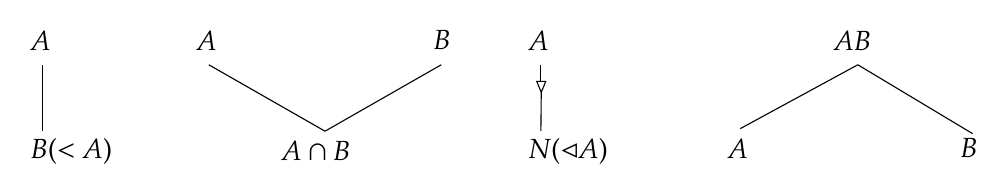
\begin{tikzpicture}[x=0.75pt,y=0.75pt,yscale=-1,xscale=1]
%uncomment if require: \path (0,476); %set diagram left start at 0, and has height of 476

%Straight Lines [id:da7779001782086632] 
\draw    (160,128) -- (160,160) ;
%Straight Lines [id:da022889284236344398] 
\draw    (240,128) -- (296,160) ;
%Straight Lines [id:da2566202829190811] 
\draw    (352,128) -- (296,160) ;
%Straight Lines [id:da7740882134647555] 
\draw    (400,128) -- (400,136) ;
%Shape: Triangle [id:dp2935044745325599] 
\draw   (400.17,141.33) -- (398,136) -- (402.33,136) -- cycle ;
%Straight Lines [id:da22801314938737094] 
\draw    (400.17,141.33) -- (400,160) ;
%Straight Lines [id:da18421896184725317] 
\draw    (608,161.19) -- (552.7,128) ;
%Straight Lines [id:da6071802710840233] 
\draw    (496.03,158.79) -- (552.7,128) ;

% Text Node
\draw (153,110.4) node [anchor=north west][inner sep=0.75pt]    {$A$};
% Text Node
\draw (153,162.4) node [anchor=north west][inner sep=0.75pt]    {$B( < A)$};
% Text Node
\draw (233,110.4) node [anchor=north west][inner sep=0.75pt]    {$A$};
% Text Node
\draw (347,110.4) node [anchor=north west][inner sep=0.75pt]    {$B$};
% Text Node
\draw (274,163.4) node [anchor=north west][inner sep=0.75pt]    {$A\cap B$};
% Text Node
\draw (393,110.4) node [anchor=north west][inner sep=0.75pt]    {$A$};
% Text Node
\draw (393,162.4) node [anchor=north west][inner sep=0.75pt]    {$N( \lhd A)$};
% Text Node
\draw (489,162.4) node [anchor=north west][inner sep=0.75pt]    {$A$};
% Text Node
\draw (601,162.4) node [anchor=north west][inner sep=0.75pt]    {$B$};
% Text Node
\draw (540,110.4) node [anchor=north west][inner sep=0.75pt]    {$AB$};


\end{tikzpicture}
\end{center}
Now we show that we have the figure below:
\begin{center}


\tikzset{every picture/.style={line width=0.75pt}} %set default line width to 0.75pt        

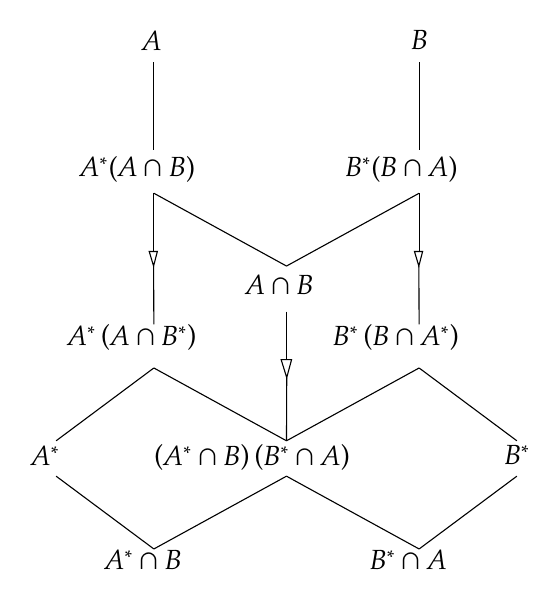
\begin{tikzpicture}[x=0.75pt,y=0.75pt,yscale=-1,xscale=1]
%uncomment if require: \path (0,476); %set diagram left start at 0, and has height of 476

%Straight Lines [id:da1285470564836515] 
\draw    (260.84,147.64) -- (260.84,189.73) ;
%Straight Lines [id:da05078319732728209] 
\draw    (388.64,147.64) -- (388.64,189.73) ;
%Straight Lines [id:da09780746468402302] 
\draw    (260.84,210.77) -- (324.74,245.85) ;
%Straight Lines [id:da17745847701647044] 
\draw    (388.64,210.77) -- (324.74,245.85) ;
%Straight Lines [id:da5095576644106456] 
\draw    (260.84,210.77) -- (260.84,238.84) ;
%Shape: Triangle [id:dp5891558957390246] 
\draw   (260.7,245.85) -- (258.6,238.84) -- (262.52,238.84) -- cycle ;
%Straight Lines [id:da7840217059124364] 
\draw    (260.7,245.85) -- (260.84,273.91) ;
%Straight Lines [id:da40595121864678196] 
\draw    (388.64,210.77) -- (388.64,238.84) ;
%Shape: Triangle [id:dp4463057230026377] 
\draw   (388.5,245.85) -- (386.4,238.84) -- (390.32,238.84) -- cycle ;
%Straight Lines [id:da9773677511142567] 
\draw    (388.5,245.85) -- (388.64,273.91) ;
%Straight Lines [id:da3598676892182031] 
\draw    (324.74,267.78) -- (324.74,290.92) ;
%Straight Lines [id:da7359728450021898] 
\draw    (260.84,294.96) -- (324.74,330.04) ;
%Straight Lines [id:da9152351124333524] 
\draw    (388.64,294.96) -- (324.74,330.04) ;
%Straight Lines [id:da7071342895580122] 
\draw    (213.75,330.04) -- (260.84,294.96) ;
%Straight Lines [id:da7370646140530484] 
\draw    (388.64,294.96) -- (435.73,330.04) ;
%Straight Lines [id:da6592447901565566] 
\draw    (213.75,347.09) -- (260.84,382.16) ;
%Straight Lines [id:da830254473944666] 
\draw    (388.64,382.16) -- (435.73,347.09) ;
%Straight Lines [id:da9011367137466262] 
\draw    (324.74,347.09) -- (260.84,382.16) ;
%Straight Lines [id:da7677251177508744] 
\draw    (324.74,347.09) -- (388.64,382.16) ;
%Shape: Triangle [id:dp47542625091877366] 
\draw   (324.85,299.6) -- (322.15,290.91) -- (327.19,290.91) -- cycle ;
%Straight Lines [id:da12771942521241186] 
\draw    (324.85,299.6) -- (324.74,330.04) ;

% Text Node
\draw (253.84,131.27) node [anchor=north west][inner sep=0.75pt]    {$A$};
% Text Node
\draw (383.48,131.27) node [anchor=north west][inner sep=0.75pt]    {$B$};
% Text Node
\draw (223.84,191.71) node [anchor=north west][inner sep=0.75pt]    {$A^{*}( A\cap B)$};
% Text Node
\draw (351.88,191.71) node [anchor=north west][inner sep=0.75pt]    {$B^{*}( B\cap A)$};
% Text Node
\draw (303.66,248.78) node [anchor=north west][inner sep=0.75pt]    {$A\cap B$};
% Text Node
\draw (217.92,272.84) node [anchor=north west][inner sep=0.75pt]    {$A^{*}\left( A\cap B^{*}\right)$};
% Text Node
\draw (345.88,272.84) node [anchor=north west][inner sep=0.75pt]    {$B^{*}\left( B\cap A^{*}\right)$};
% Text Node
\draw (259.74,330.72) node [anchor=north west][inner sep=0.75pt]    {$\left( A^{*} \cap B\right)\left( B^{*} \cap A\right)$};
% Text Node
\draw (200.31,331.15) node [anchor=north west][inner sep=0.75pt]    {$A^{*}$};
% Text Node
\draw (428.41,331.15) node [anchor=north west][inner sep=0.75pt]    {$B^{*}$};
% Text Node
\draw (235.84,381.52) node [anchor=north west][inner sep=0.75pt]    {$A^{*} \cap B$};
% Text Node
\draw (363.64,381.52) node [anchor=north west][inner sep=0.75pt]    {$B^{*} \cap A$};


\end{tikzpicture}
\end{center}
The subgroups are trivial. Also observed that 
$$
A^*\left( A\cap B^* \right) \cap \left( A\cap B \right) =\left( A^*\cap B \right) \left( B^*\cap A \right) =\left( A\cap B \right) \cap \left( A^*\cap B \right) B^*
$$
and 
$$
A^*\cap \left( A^*\cap B \right) \left( B^*\cap A \right) =A^*\cap B,B^*\cap \left( B^*\cap A \right) \left( A^*\cap B \right) =B^*\cap A,
$$
we have the intersections to be true. Now for the normal subgroups, we observe that 
$$
B^*\lhd B\Rightarrow B\cap B^*\lhd A\cap B\Rightarrow A^*\left( A\cap B^* \right) \lhd A^*\left( A\cap B \right) 
$$
and 
$$
A^*\lhd A\Rightarrow A\cap A^*\lhd A\cap B\Rightarrow B^*\left( B\cap A^* \right) \lhd B^*\left( A\cap B \right) ,
$$
hence the normal subgroups are true. Now consider the parallelogram in the diagram, we have isomorphisms by the Second Isomorphism Theorem: 
$$
A^*\left( A\cap B \right) /A^*\left( A\cap B^* \right) \cong B^*\left( A\cap B \right) /B^*\left( A^*\cap B \right) \cong \left( A\cap B \right) /\left( A^*\cap B \right) \left( B^*\cap A \right) .
$$
\end{proof}
\begin{note}\em
This lemma has another name of the \textbf{Butterfly Lemma}, since the diagram above is similar to a butterfly.
\end{note}
\begin{theorem}(Schreier)
Any two subnormal [resp.normal] series of a group $G$ has subnormal [resp.normal] refinements that are equivalent.
\end{theorem}
\begin{proof}
Let $G=G_0>G_1>\cdots >G_n$ and $G=H_0>H_1>\cdots >H_m$ be two subnormal [resp.normal] series of $G$. For all $0\le i\le n$ consider the following series: 
$$
G_i=G_{i+1}\left( G_i\cap H_0 \right) >G_{i+1}\left( G_i\cap H_1 \right) >\cdots >G_{i+1}\left( G_i\cap H_m \right) >G_{i+1}\left( G_i\cap H_{m+1} \right) =G_{i+1},
$$
where $G_{n+1}=H_{m+1}=\left< e \right> $, then by Zassenhaus' Lemma we have $G_{i+1}\left( G_i\cap H_{j+1} \right) \lhd G_{i+1}\left( G_i\cap H_j \right) $ [if the original series are normal, then observe that $G_i\lhd G,H_j\lhd G\Rightarrow G_i\cap H_j\lhd G$, $G_{i+1}\lhd G$ and $G_{i+1}\left( G_i\cap H_j \right) =G_{i+1}\lor \left( G_i\cap H_j \right) \lhd G$]. Inserting these groups between $G_i$ and $G_{i+1}$ for all $0\le i\le n$, and denote $G\left( i,j \right) =G_{i+1}\left( G_i\cap H_j \right) $, we have 
$$
G=G\left( 0,0 \right) >G\left( 0,1 \right) >\cdots >G\left( 0,m \right) >\cdots >G\left( n,0 \right) >\cdots >G\left( n,m \right) .
$$
Similarly we may have the refinement of $G=H_0>H_1>\cdots >H_m$ as 
$$
G=H\left( 0,0 \right) >H\left( 1,0 \right) >\cdots >H\left( n,0 \right) >\cdots >H\left( 0,m \right) >\cdots >H\left( n,m \right) ,
$$
It is easy to see that the two series above has the same number of terms $(n+1)(m+1)$. For each pair $(i,j)$ again by Zassenhaus' Lemma we have 
$$
\frac{G\left( i,j \right)}{G\left( i,j+1 \right)}=\frac{G_{i+1}\left( G_i\cap H_j \right)}{G_{i+1}\left( G_i\cap H_{j+1} \right)}\cong \frac{H_{j+1}\left( G_i\cap H_j \right)}{H_{j+1}\left( G_{i+1}\cap H_j \right)}=\frac{H\left( i,j \right)}{H\left( i+1,j \right)},
$$
therefore we finished our proof.
\end{proof}
\begin{theorem}(Jordan-Holder)
Any two composition series of a group $G$ are equivalent. Therefore every group having a composition series determines a unique list of simple groups.
\end{theorem}
\begin{proof}
Since composition series are subnormal series, by Schreier's Theorem we know that every two composition series have equivalent refinements. But every refinement of a composition series is equivalent to itself, then any two composition series are equivalent.
\end{proof}
\begin{note}\em
The theorem does not state the existence of a composition series for a given group.
\end{note}
The Jordan-Holder Theorem indicates that some knowledge of simple groups might be useful. The classification of all finite simple groups have been finished in 1981, which is based on the work of a large number of group theorists. We may note that non-abelian simple groups of small order are quite rare. There are only two non-abelian simple groups of order less than 200: $A_5$ and a subgroup of $S_7$ of order $168$.
\begin{center}
\begin{large}
    \textbf{Exercises for 3.6}
\end{large}
\end{center}
\begin{problem}\em
If $G=G_0>G_1>\cdots>G_n$ is a subnormal series of a finite group $G$, then $|G|=\left(\prod_{i=0}^{n-1}|G_i/G_{i+1}|\right)|G_n|$.
\end{problem}
\begin{proof}
We observed that 
$$
\left( \prod_{i=0}^{n-1}{\left| G_i/G_{i+1} \right|} \right) \left| G_n \right|=\left( \prod_{i=0}^{n-1}{\left[ G_i:G_{i+1} \right]} \right) \left| G_n \right|=\left[ G_0:G_n \right] \left| G_n \right|=\left| G_0 \right|=\left| G \right|.
$$
\end{proof}
\begin{problem}\em
If $N$ is a simple normal subgroup of a group $G$ and $G/N$ has a composition series, then $G$ has a composition series.
\end{problem}
\begin{proof}
Consider the composition series $G/N=G_0/N>G_1/N>\cdots >G_n/N=\left< e_{G/N} \right> $, from which we have a subnormal series of $G$, which is $G=G_0>G_1>\cdots >G_n$. By the Third Isomorphism Theorem we have $G_i/G_{i+1}\cong \left( G_i/N \right) /\left( G_{i+1}/N \right) $ is a simple group, therefore the series $G=G_0>G_1>\cdots >G_n$ is a composition series.
\end{proof}
\begin{problem}\em
A composition series of a group is a subnormal series of maximal (finite) length.
\end{problem}
\begin{proof}
Let $G$ be a group and $G=G_0>G_1>\cdots >G_n$ be a composition series of $G$. If there exists some series $G=G_0^\prime>G_1^\prime>\cdots >G_m^\prime$ whose length is longer than $G=G_0>G_1>\cdots >G_n$, then the new series is a refinement of the original series. However the refinement of a composition series is equivalent to itself, which is a contradict!
\end{proof}
\begin{problem}\em
An abelian group has a composition series if and only if it is finite.
\end{problem}
\begin{proof}
Let $G$ be a finite abelian group, Then it is finite and hence has a composition series. Conversely, let $G$ be an abelian group and $G=G_0>G_1>\cdots>G_n$ be a composition series of $G$. Then each $G_i/G_{i+1}$ is abelian and simple, therefore it is finite cyclic and has prime order. By exercise 3.60 we may conclude that $G$ is finite, therefore $G$ is finite abelian.
\end{proof}
\begin{problem}\em
If $H\lhd G$, where $G$ has a composition series, then $G$ has a composition series one of whose terms is $H$.
\end{problem}
\begin{proof}
Let $G=G_0>G_1>\cdots >G_n$ be a composition series of $G$. Then consider the normal series $G>H>\left< e \right> $, which is either or not a composition series. If it is a composition series, then we are done. If not, by Schreier's Theorem we have a subnormal series $G=N_0>N_1>\cdots >N_r=\left< e \right> $ which is a refinement of both $G=G_0>G_1>\cdots >G_n$ and $G>H>\left< e \right> $. Clearly there exists some $N_i=H$. Now we show that the new series is a composition series. Note that there is no proper refinement of a composition series and hence $G=N_0>N_1>\cdots >N_r=\left< e \right> $ is equivalent to the original series and we finished our proof.
\end{proof}
\begin{problem}\em
A solvable group with a composition series is finite.
\end{problem}
\begin{proof}
Let $G$ be a solvable group and $G=G_0>G_1>\cdots >G_n$ be a composition series. Since $G$ is solvable, it has a solvable series $G=H_0>H_1>\cdots >H_m$. Consider the refinement of these two series, which is equivalent by Schreier's Theorem. We denote the new series as $G=N_0>N_1>\cdots >N_r$, which is the refinement of a solvable series and hence solvable. Also it is the refinement of a composition series, which is equivalent to itself. Therefore the new series is both composition and solvable series, hence $N_i/N_{i+1}$ is abelian and simple, therefore isomorphic to cyclic group of prime order. By exercise 3.60 we know that $G$ is of finite order.
\end{proof}
\begin{problem}\em
If $H$ and $K$ are solvable subgroups of $G$ with $H\lhd G$, then $HK$ is a solvable subgroup of $G$.
\end{problem}
\begin{proof}
By Theorem 3.46 we know that $G$ is solvable if and only if $N$ and $G/N$ is solvable, where $N$ is normal in $G$. Now consider $HK$. Clearly $H\lhd HK$, and by the Second Isomorphism Theorem we have $HK/K\cong H/(H\cap K)$, which is solvable since every quotient and subgroup of a solvable group is also solvable. Therefore $HK$ is solvable by Theorem 3.46.
\end{proof}
\begin{problem}\em
A group $G$ is nilpotent if and only if there is a normal series $G=G_0>G_1>\cdots>G_n=\left<e\right>$ such that $G_i/G_{i+1}<C(G/G_{i+1})$ for every $i$.
\end{problem}
\begin{proof}
If $G$ is nilpotent, we have shown that $C_i\left( G \right) /C_{i+1}\left( G \right) =C\left( G/C_{i+1}\left( G \right) \right) $, which its central chain is a normal series satisfies the condition. Conversely, let $\left< e \right> <G_1<G_2<\cdots <G_n$ be a normal series with $G_i/G_{i-1}<C\left( G/G_{i-1} \right) $, we show that $G$ is nilpotent by proving $G_i<C_i\left( G \right) $ by induction. For $i=1$, we observe $G_1=G_1/G_0<C\left( G/G_0 \right) =C\left( G \right) =C_1\left( G \right) $ and the result holds. Now suppose this is true for $k$, now consider $k+1$. Define the map $G/G_{k}\to G/C_k(G)$ and consider the image of $C(G/G_k)$, which maps into $C_{k+1}(G)/C_k(G)$. Thus every element in $G_{k+1}$ maps into $C_{k+1}(G)$ and we finished our proof.
\end{proof}
\begin{problem}\em
Prove the Fundamental Theorem of Arithmetic by Jordan-Holder's Theorem.
\end{problem}
\begin{proof}
Let $n=p_1p_2\cdots p_k=q_1q_2\cdots q_s$. We show that for all $i$ there exists some $j$ such that $p_i=q_j$. We observe the following composition series: 
$$
\mathbb{Z} /n\mathbb{Z} >\mathbb{Z} /\left( \frac{n}{p_1} \right) \mathbb{Z} >\mathbb{Z} /\left( \frac{n}{p_1p_2} \right) \mathbb{Z} >\cdots >\mathbb{Z} /\left( \frac{n}{p_1p_2\cdots p_k} \right) \mathbb{Z} =\left\{ 1 \right\} 
$$
and 
$$
\mathbb{Z} /n\mathbb{Z} >\mathbb{Z} /\left( \frac{n}{q_1} \right) \mathbb{Z} >\mathbb{Z} /\left( \frac{n}{q_1q_2} \right) \mathbb{Z} >\cdots >\mathbb{Z} /\left( \frac{n}{q_1q_2\cdots q_s} \right) \mathbb{Z} =\left\{ 1 \right\} ,
$$
which are suppose to be equivalent by Jordan-Holder's Theorem, therefore the composition of the integer $n$ is unique and we finished our proof.
\end{proof}
\subsection{Postscript on Group Theory}
We end our discussion in group theory with a full classification of groups of small order. We only present the classification of groups with orders $\leq 15$ (as shown in the table below). In the "Reference" column, "[G]Corollary 6.2" refers to Corollary 6.2 in GTM73, while the other entries without [G] indicate references to the main text of the notes.
$$
\begin{matrix}
	\mathrm{Order}&		\mathrm{Distinct} \mathrm{Groups}&		\mathrm{Reference}\\
	1&		\left< e \right>&		\cdots\\
	2&		\mathbb{Z} _2&		\mathrm{Exercise}2.42\\
	3&		\mathbb{Z} _3&		\mathrm{Exercise}2.42\\
	4&		\mathbb{Z} _4,\mathbb{Z} _2\oplus \mathbb{Z} _2&		\mathrm{Exercise}2.44\\
	5&		\mathbb{Z} _5&		\mathrm{Exercise}2.42\\
	6&		\mathbb{Z} _6,D_3&		\left[ \mathrm{G} \right] \mathrm{Corollary}6.2\\
	7&		\mathbb{Z} _7&		\mathrm{Exercise}2.42\\
	8&		\mathbb{Z} _2\oplus \mathbb{Z} _2\oplus \mathbb{Z} _2,\mathbb{Z} _2\oplus \mathbb{Z} _4,\mathbb{Z} _8,Q_8,D_4&		\mathrm{Theorem}3.7,\left[ \mathrm{G} \right] \mathrm{Corollary}6.2\\
	9&		\mathbb{Z} _3\oplus \mathbb{Z} _3,\mathbb{Z} _9&		\mathrm{Exercise}3.51,\left[ \mathrm{G} \right] \mathrm{Corollary}6.2\\
	10&		\mathbb{Z} _{10},D_5&		\mathrm{Theorem}3.7\\
	11&		\mathbb{Z} _{11}&		\mathrm{Exercise}2.42\\
	12&		\mathbb{Z} _2\oplus \mathbb{Z} _6,\mathbb{Z} _{12},A_4,D_6,T&		\mathrm{Theorem}3.7,\left[ \mathrm{G} \right] \mathrm{Proposition}6.4\\
	13&		\mathbb{Z} _{13}&		\mathrm{Exercise}2.42\\
	14&		\mathbb{Z} _{14},D_7&		\left[ \mathrm{G} \right] \mathrm{Corollary}6.2\\
	15&		\mathbb{Z} _{15}&		\left[ \mathrm{G} \right] \mathrm{Proposition}6.1\\
\end{matrix}
$$
\newpage
\section{Rings}
Another fundamental concept in the study of algebra is that of a ring. The problem of classifying all rings up to isomorphism is far more complicated than the corresponding problem for groups. We only introduce some basic facts about rings that are most frequently used in several areas of algebra.
\subsection{Rings and Homomorphisms}
The basic concepts in the theory of rings are defined and numerous examples are given in this section.
\begin{definition}
A \textbf{ring} is a nonempty set $R$ together with two binary operations, usually denote as addition and multiplication, such that\par
(i) $(R,+)$ is an abelian group,\par
(ii) $(ab)c=a(bc)$ for all $a,b,c\in R$,\par
(iii) $a(b+c)=ab+ac$ and $(a+b)c=ac+bc$.\par
If in addition,\par
(iv) $ab=ba$ for all $a,b\in R$,\par
then $R$ is said to be a \textbf{commutative ring}. If $R$ contains an element $1_R$ such that\par
(v) $1_Ra=a1_R=a$ for all $a\in R$,\par
then $R$ is said to be a \textbf{ring with identity}.
\end{definition}
\begin{note}\em
The symbol $1_R$ will also denote the identity map $1_R:R\to R$. This will not cause ambiguity in context.
\end{note}
The additive identity element of a ring is denoted as $0$. If $R$ is a ring, then $na$ has its usual meaning as $a+a+\cdots+a$ ($n$ summonds) when $n>0$. We first list some basic properties of a ring:
\begin{theorem}
Let $R$ be a ring. Then\par
(i) $0a=a0=0$ for all $a\in R$;\par
(ii) $(-a)b=a(-b)=-(ab)$ for all $a,b\in R$;\par
(iii) $(-a)(-b)=ab$ for all $a,b\in R$;\par
(iv) $(na)b=a(nb)=n(ab)$ for all $n\in\mathbb{Z}$ and $a,b\in R$;\par
(v) $\left(\sum_{i=1}^na_i\right)\left(\sum_{j=1}^mb_j\right)=\sum_{i=1}^n\sum_{j=1}^ma_ib_j$ for all $a_i,b_j\in R$.
\end{theorem}
\begin{proof}
(i) Observed that $ab=a(b+0)=ab+a0$, then $a0=0$. Analogously we may show that $0a=0$.\par
(ii) By (i) we know that $(a+(-a))b=0b=0$, therefore $ab+(-a)b=0$. Hence $(-a)b=-ab$. Analogously we may show that $a(-b)=-ab$.\par
(iii) Observed that $(-a)(-b)=-(a(-b))=-(-ab)=ab$.\par
(iv) We prove by induction. Indeed it suffices to show $(2a)b=2ab$, which follows by $(a+a)b=ab+ab=2ab$.\par
(v) We prove by induction on $m$. If $m=1$, then by (iv) we have $\left( \sum_{i=1}^n{a_i} \right) b_1=\sum_{i=1}^n{a_ib_1}$. Now if the condition holds for $m-1$, we have 
$$
\left( \sum_{i=1}^n{a_i} \right) \left( \sum_{j=1}^m{b_j} \right) =b_m\left( \sum_{i=1}^n{a_i} \right) +\left( \sum_{i=1}^n{a_i} \right) \left( \sum_{j=1}^{m-1}{b_j} \right) =\sum_{i=1}^n{\sum_{j=1}^m{a_ib_j}}.
$$
Then we finished our proof.
\end{proof}
The next definitions introduce some more terminology, after which some examples will be given.
\begin{definition}
A nonzero element $a$ in a ring $R$ is said to be a \textbf{left zero divisor} [resp. right] if there exists a nonzero $b\in R$ such that $ab=0$ [resp. $ba=0$]. A \textbf{zero divisor} is an element of $R$ which is both a left and right zero divisor.
\end{definition}
It is easy to verify that a ring $R$ has no zero divisor if and only if the cancellation holds in $R$, since if $a$ is a zero divisor of $R$, then there exists nonzero $b,c$ such that $ab=ca=0$. Since $a\ne 0$, by cancellation and $ab=a0$ we have $b=0$,a contradiction! Similarly we conclude that $c=0$.
\begin{definition}
An element $a$ in a ring $R$ with identity is said to be \textbf{left invertible} [resp. right] if there exists $c\in R$[resp. $b\in R$] such that $ca=1_R$ [resp. $ab=1_R$]. The element $c$ [resp. b] is called a \textbf{left inverse} [resp. right] of $a$. An element $a\in R$ that is both left and right invertible is said to be \textbf{invertible} or to be a \textbf{unit}.
\end{definition}
\begin{note}\em
(i) The left and right inverses of a unit $a$ in a ring with identity necessarily coincide, since 
$$
ab=ca=1_R\Rightarrow b=1_Rb=\left( ca \right) b=c\left( ab \right) =c1_R=c.
$$\par
(ii) The set of units in a ring $R$ forms a group under multiplication.
\end{note}
\begin{definition}
A commutative ring $R$ with identity $1_R\ne 0$ and no zero divisors is called a \textbf{integral domain}. A ring $D$ with identity $1_D\ne 0$ in which every nonzero element is a unit is called a \textbf{division ring}. A \textbf{field} is a commutative division ring.
\end{definition}
\begin{note}\em
(i) Every integral domain and every division ring has at least two elements, namely $0$ and $1_R$.\par
(ii) A ring $R$ with identity is a division ring if and only if the nonzero elements of $R$ form a group under multiplication. See Remark 4.2 (ii).\par
(iii) Every field $F$ is an integral domain since $ab=0$ and $a\ne 0$ imply that $b=1_Fb=(a^{-1}a)b=a^{-1}(ab)=a^{-1}0=0$.
\end{note}
Now we give some examples.
\begin{example}\em
(i) The ring $\mathbb{Z}$ is an integral domain. First $ab=ba$ for all $a,b\in\mathbb{Z}$, hence $\mathbb{Z}$ is a commutative ring. Now we show that $\mathbb{Z}$ has no divisor. Let $ab=0$ and $a\ne 0$, then $b=0$.\par
(ii) The set $E$ of even integers is a commutative ring without identity.\par
(iii) Each of $\mathbb{Q}$, $\mathbb{R}$ and $\mathbb{C}$ is a field under usual addition and multiplication.\par
(iv) The $n\times n$ matrices over $\mathbb{Q}$ or $\mathbb{R}$ or $\mathbb{C}$ form a non-commutative ring with identity. The units in this ring are precisely the non-singular matrices.
\end{example}
\begin{example}\em
For each positive integer $n$, the set $\mathbb{Z}_n$ of integers modulo $n$ is a ring. Clearly $\mathbb{Z}_n$ is an abelian additive group, and is a semi-group under multiplication. If $n$ is not prime, say $n=kr$ with $k,r>1$, then $\overline{k}\ne\overline{0}$, $\overline{r}\ne\overline{0}$, while $\overline{k}\overline{r}=\overline{kr}=\overline{0}$, hence $\overline{k}$ and $\overline{r}$ are zero divisors. If $n$ is prime, then $\mathbb{Z}_n$ is a field by Exercise 2.5.
\end{example}
\begin{example}\em
Let $A$ be an abelian group and $\mathrm{End}A$ be the endomorphisms $f:A\to A$. Define addition in $\mathrm{End}A$ by $(f+g)(a)=f(a)+g(a)$. Then $\mathrm{End}A$ is an abelian group under addition. Let the multiplication in $\mathrm{End}A$ be the composition of homomorphisms, then $\mathrm{End}A$ is a (possibly non-commutative) ring with identity $1_A:A\to A$.
\end{example}
\begin{example}\em
Let $G$ be a multiplicative group and $R$ a ring. Let $R(G)$ be the additive abelian group $\bigoplus_{g\in G}R$. It will be convenient to adopt a new notion for the elements of $R(G)$. An element $x=\{r_g\}_{g\in G}$ of $R(G)$ has only finitely many nonzero coordinates, say $r_{g_1},r_{g_2},\cdots,r_{g_n},g_i\in G$. Denote $x$ by the \textbf{formal sum} $\sum_{i=1}^nr_{g_i}g_i$. We also allow the possibility that some of the $r_{g_i}$ may be zero or that some $g_i$ are repeated, so that an element of $R(G)$ may be written in formally different ways. In this notation, addition in group $R(G)$ is given by 
$$
\sum_{i=1}^n{r_{g_i}g_i}+\sum_{i=1}^n{s_{g_i}g_i}=\sum_{i=1}^n{\left( r_{g_i}+s_{g_i} \right) g_i}.
$$
Note that by inserting some zero coefficients we may assume that two formal sums involve exactly the same indices $g_1,\cdots,g_n$. Define multiplication in $R(G)$ by 
$$
\left( \sum_{i=1}^n{r_ig_i} \right) \left( \sum_{j=1}^n{s_jh_j} \right) =\sum_{i=1}^n{\sum_{j=1}^n{\left( r_is_j \right) \left( g_ih_j \right)}},
$$
and since $r_is_j$ and $g_ih_j$ are defined respectively in $R$ and $G$, the definition above is well-defined. With these operations $R(G)$ is a ring, called the \textbf{group ring} of $G$ over $R$. $R(G)$ is commutative if and only if both $R$ and $G$ are commutative. If $R$ has identity $1_R$ and $e$ is the identity element of $G$, then $1_Re$ is the identity of $R(G)$.
\end{example}
\begin{example}\em
Let $\mathbb{R}$ be the field of real numbers and $S$ be the set of symbols $1,i,j,k$. Let $K$ be the additive abelian group $\mathbb{R}\oplus\mathbb{R}\oplus\mathbb{R}\oplus\mathbb{R}$ and write the elements of $K$ as formal sums $(a_0,a_1,a_2,a_3)=a_01+a_1i+a_2j+a_3k$. We adopt the conventions that $a_01\in K$ is identified with $a_0\in\mathbb{R}$ and the terms with zero coefficients may be omitted. For example, $4+2j=a\cdot1+0i+2j+0k$. Then we say 
$$
a_01+a_1i+a_2j+a_3k=b_01+b_1i+b_2j+b_3k
$$
if and only if $a_i=b_i$ for all $i=0,1,2,3$. Define the addition 
\begin{small}
$$
\left( a_01+a_1i+a_2j+a_3k \right) +\left( b_01+b_1i+b_2j+b_3k \right) =\left( a_0+b_0 \right) 1+\left( a_1+b_1 \right) i+\left( a_2+b_2 \right) j+\left( a_3+b_3 \right) k,
$$
\end{small}
and the multiplication 
$$
\begin{aligned}
\left( a_01+a_1i+a_2j+a_3k \right) \left( b_01+b_1i+b_2j+b_3k \right) &=\left( a_0b_0=a_1b_1-a_2b_2-a_3b_3 \right) 
\\
&+\left( a_0b_1+a_1b_0+a_2b_3-a_3b_2 \right) i
\\
&+\left( a_0b_2+a_2b_0+a_3b_1-a_1b_3 \right) j
\\
&+\left( a_0b_3+a_3b_0+a_1b_2-a_2b_1 \right) k,
\end{aligned}
$$
the product formula is obtained by multiplying the formal sums term by term subject to the following relations:\par
(i) $i^2=j^2=k^2=ijk=-1$;\par
(ii) $ij=-ji=k$, $jk=-jk=i$, $ki=-ik=j$.\par
Under the product $K$ is a non-commutative division ring in which the multiplicative inverse of $a_0+a_1i+a_2j+a_3k$ is the following:
$$
\frac{a_0}{d}-\frac{a_1}{d}i-\frac{a_2}{d}j-\frac{a_3}{d}k,d=a_{0}^{2}+a_{1}^{2}+a_{2}^{2}+a_{3}^{2}.
$$
$K$ is called the division ring of \textbf{real quaternions}. The quaternions may also be interpreted as a certain subring of the ring of all $2\times 2$ matrices over the field $\mathbb{C}$ of complex numbers.
\end{example}
Definition 4.1 shows that under multiplication the element of a ring $R$ actually form a semi-group. Therefore we may define the product as follows: for each $a\in R$ and $n\in\mathbb{N}_+$, $a^n=a\times a\times\cdots\times a$($n$ factors) and $a^0=1_R$ if $R$ has an identity. Similarly we have $a^{m+n}=a^m\cdot a^n$. Subtraction in a ring $R$ is defined in the usually way: $a-b=a+(-b)$. Clearly $a(b-c)=ab-ac$ and $(a-b)c=ac-bc$ for all $a,b,c\in R$.\par
The next theorem is frequently useful in computations. Recall that if $k$ and $n$ are integers with $0\le k\le n$, then the \textbf{binomial coefficient} $\left( \begin{array}{c}
	n\\
	k\\
\end{array} \right) $ is the number $\frac{n!}{k!(n-k)!}$, where $0!=1$ and $n!=n(n-1)\cdots 2\cdot1$ for all $n\in\mathbb{N}_+$.
\begin{theorem}(Binomial Theorem)
Let $R$ be a ring with identity, $n$ is a positive integer, and $a,b,a_1,a_2,\cdots,a_n\in R$.\par
(i) If $ab=ba$, then $
\left( a+b \right) ^n=\sum_{k=1}^n{\left( \begin{array}{c}
	n\\
	k\\
\end{array} \right) a^kb^{n-k}}.
$\par
(ii) If $a_ia_j=a_ja_i$, then 
$$
\left( \sum_{i=1}^s{a_i} \right) ^n=\sum{\frac{n!}{\left( i_1! \right) \left( i_2! \right) \cdots \left( i_s! \right)}\prod_{i=1}^s{a_{i}^{i_i}}},
$$
where the sum is taken over all $s$-tuples $(i_1,i_2,\cdots,i_s)$ such that $i_1+i_2+\cdots+i_s=n$.
\end{theorem}
The proof of which is similar to that of real numbers, since the elements we are discussing here commutes. We skip the proof of such a theorem.
\begin{definition}
Let $R$ and $S$ be rings. A function $f:R\to S$ is a \textbf{homomorphism of rings} provided that for all $a,b\in R$,
$$f(a+b)=f(a)+f(b),\hspace{1cm}f(ab)=f(a)f(b).$$
\end{definition}
\begin{note}\em
It is easy to see that all the rings and ring homomorphisms forms a concrete category.
\end{note}
Similar to group homomorphisms, some terminologies are also used here: a \textbf{monomorphism} [resp.\textbf{epimorphism, isomorphism}] of rings is a homomorphism that is an injective [resp. surjective, bijective] map. A monomorphism of rings $R\to S$ is sometimes called an \textbf{embedding} of $R$ in $S$. An isomorphism $R\to R$ is called an \textbf{automorphism} of $R$. The \textbf{kernel} of a homomorphism of rings $f:R\to S$ is the set $\{r\in R:f(r)=0\}$ and the \textbf{image} of $f$ is the set $\{s\in S:f(r)=s\ \text{for some}\ r\in R$. Note that if $R$ and $S$ both have identity $1_R$ and $1_S$, we do not require $f(1_R)=1_S$.
\begin{example}\em
The canonical map $\mathbb{Z}\to\mathbb{Z}_m$ given by $k\mapsto\overline{k}$ is an epimorphism of rings. The map $\mathbb{Z}_3\to\mathbb{Z}_6$ given by $\overline{k}\mapsto\overline{4k}$ is a well-defined monomorphism of rings.
\end{example}
\begin{example}\em
Let $G$ and $H$ be multiplicative groups and $f:G\to H$ a homomorphism of groups. Let $R$ be a ring and define a map on group rings $\overline{f}:R(G)\to R(H)$ by 
$$\overline{f}\left(\sum_{i=1}^nr_ig_i\right)=\sum_{i=1}^nr_if(g_i),$$
then $\overline{f}$ is a homomorphism of rings.
\end{example}
\begin{definition}
Let $R$ be a ring, if there is a least positive integer $n$ such that $na=0$ for all $a\in R$, then $R$ is said to have \textbf{characteristic} $n$. If no such $n$ exists $R$ is said to have \textbf{characteristic zero}. We denote the characteristic of $R$ as $\mathrm{char}R$.
\end{definition}
We have the following theorem:
\begin{theorem}
Let $R$ be a ring with identity $1_R$ and characteristic $n>0$.\par
(i) If $\varphi:\mathbb{Z}\to R$ is the map given by $m\mapsto m1_R$, then $\varphi$ is a homomorphism of rings with kernel $\left<n\right>=\{kn:k\in\mathbb{Z}\}$.\par
(ii) $n$ is the least positive integer such that $n1_R=0$.\par
(iii) If $R$ has no zero divisors, in particular $R$ is an integral domain, then $n$ is prime.
\end{theorem}
\begin{proof}
(i) We first show that $\varphi$ is a homomorphism. This is clear since 
$$
f\left( a+b \right) =\left( a+b \right) 1_R=a1_R+b1_R=f\left( a \right) +f\left( b \right) ,\hspace{0.5cm}f\left( ab \right) =ab1_R=a1_Rb1_R=f\left( a \right) f\left( b \right) .
$$
Then since $\mathrm{char}R=n$, we have $a1_R=0$ if and only if $a=kn$, where $k$ is an integer. Therefore $\mathrm{Ker}f=\left<n\right>$.\par
(ii) Let $a<n$ and $a1_R=0$. Then for all $b\in R$, we have 
$$
a1_Rb=a\left( 1_Rb \right) =ab=0b=0,
$$
hence $\mathrm{char}R=a$, which is a contradiction!\par
(iii) If $n=rk$, where $r<n$, $k<n$, then 
$$
n1_R=\left( kr \right) 1_R1_R=\left( k1_R \right) \left( r1_R \right) =0,
$$
since $R$ has no divisor, we have $k1_R=0$ or $r1_R=0$, which contradict to (ii) and hence $n$ is prime.
\end{proof}
\begin{theorem}
Every ring $R$ may be embedded in a ring $S$ with identity. The ring $S$ (which is not unique) may be chosen to be either of characteristic zero or of the same characteristic as $R$.
\end{theorem}
\begin{proof}
If $\mathrm{char}S=0$, we define $S=R\oplus\mathbb{Z}$ with multiplication below:
$$
\left( r_1,k_1 \right) \left( r_2,k_2 \right) =\left( r_1r_2+k_2r_1+k_1r_2,k_1k_2 \right) ,r_i\in R,k_i\in \mathbb{Z} .
$$
Then we may verify that $S$ is a ring with identity $(0,1)$ and characteristic zero. Let $R\to S$ given by $r\mapsto(r,0)$, which is an embedding. If $\mathrm{char}S=\mathrm{char}R=n$, then define $S=R\oplus\mathbb{Z}_n$ with multiplication below:
$$
\left( r_1,\overline{k_1} \right) \left( r_2,\overline{k_2} \right) =\left( r_1r_2+\overline{k_2}r_1+\overline{k_1}r_2,\overline{k_1k_2} \right) ,r_i\in R,\overline{k_i}\in \mathbb{Z} _n.
$$
Then $\mathrm{char}S=n$ and the map $R\to S$ given by $r\mapsto(r,0)$ is an embedding.
\end{proof}
\begin{center}
\begin{large}
    \textbf{Exercises for 4.1}
\end{large}
\end{center}
\begin{problem}\em
(a) Let $G$ be an additive abelian group, define an operation of multiplication in $G$ by $ab=0$ for all $a,b\in G$. Then $G$ is a ring.\par
(b) Let $S$ be the set of all subsets of some fixed set $U$. For $A,B\in S$, define $A+B=(A-B)\cup(B-A)$ and $AB=A\cap B$. Then $S$ is a ring. Is $S$ commutative? Does it have an identity?
\end{problem}
\begin{proof}
(a) Clearly $abc=a(bc)=0$, $(a+b)c=ac+bc=0$ and $a(b+c)=ab+ac=0$ for all $a,b,c\in G$, therefore $G$ is a ring.\par
(b) We first show that $S$ is an abelian group under addition. Clearly $S$ is a group, and 
$$
A+B=\left( A-B \right) \cup \left( B-A \right) =\left( B-A \right) \cup \left( A-B \right) =B+A,
$$
therefore $S$ is abelian. Now we show that $ABC=A(BC)$, which suffices to observe that 
$$
A\cap B\cap C=A\cap \left( B\cap C \right) .
$$
Lastly, we have 
$$
\left( A+B \right) C=\left( A-B \right) \cup \left( B-A \right) \cap C=\left( \left( A\cap C \right) -\left( B\cap C \right) \right) \cup \left( \left( B\cap C \right) -\left( A\cap C \right) \right) ,
$$
therefore $(A+B)C=AC+BC$. Similarly we have $A(B+C)=AB+AC$ and we finished our proof.
\end{proof}
\begin{problem}\em
Let $\{R_i:i\in I\}$ be the family of rings with identity. Make the direct sum of abelian groups $\bigoplus_{i\in I}R_i$ into a ring by defining multiplication coordinatewise. Does $\bigoplus_{i\in I}R_i$ has an identity?
\end{problem}
\begin{proof}
We define the multiplication as follows: 
$$(a_1,a_2,\cdots)(b_1,b_2,\cdots)=(a_1a_2,b_1b_2,\cdots),a_i,b_i\in R_i.$$
Then $\bigoplus_{i\in I}R_i$ is easy to verify a ring with identity $(1_1,1_2,\cdots)$, where $1_i$ denote the identity of $R_i$.
\end{proof}
\begin{problem}\em
A ring $R$ such that $a^2=a$ for all $a\in R$ is called a \textbf{Boolean ring}. Prove that every Boolean ring $R$ is commutative and $a+a=0$ for all $a\in R$.
\end{problem}
\begin{proof}
We first show that $a=-a$ in a Boolean ring, which follows by 
$$
-a=\left( -a \right) ^2=\left( -a \right) \left( -a \right) =a^2=a.
$$
Hence $a+a=a-a=0$. Note that 
$$
a+b=\left( a+b \right) ^2=a^2+ab+ba+b^2=a+b+ab+ba,
$$
we have $ab=-ba$. But $-b=b$, hence $ab=ba$, therefore commutative.
\end{proof}
\begin{note}\em
For an example of a Boolean ring, see exercise 4.1.
\end{note}
\begin{problem}\em
Let $R$ be a ring and $S$ a nonempty set. Then the group $M(S,R)$ (see exercise 2.1) is a ring with multiplication as follows: the product of $f,g\in M(S,R)$ is the function $S\to R$ given by $s\mapsto f(s)g(s)$.
\end{problem}
\begin{proof}
By Exercise 2.1 we know that $M(S,R)$ is an abelian group since $R$ with addition is an abelian group. Now we show that $M(S,R)$ is a ring. First, clearly $fgh=f(gh)$ since 
$$f(s)g(s)h(s)=f(s)[g(s)h(s)],f,g,h\in M(S,R),s\in S.$$
Then $(f+g)h=fh+gh$ since 
$$[(f+g)h](s)=(f+g)(s)h(s)=f(s)h(s)+g(s)h(s),f,g,h\in M(S,R),s\in S.$$
Similarly we may show that $f(g+h)=fg+fh$ for all $f,g,h\in M(S,R)$ and hence $M(S,R)$ is a ring.
\end{proof}
\begin{problem}\em
If $A$ is the abelian group $\mathbb{Z}\oplus\mathbb{Z}$, then $\mathrm{End}A$ is a non-commutative ring.
\end{problem}
\begin{proof}
Consider $\phi:(a,b)\mapsto (a+a,b)$ and $\psi:(a,b)\mapsto (b,a)$. Both $\phi,\psi\in\mathrm{End}A$, but $\psi\circ\phi\ne\phi\circ\psi$.
\end{proof}
\begin{problem}\em
A finite ring with more than one element and no zero divisors is a division ring. In particular, a finite integral domain is a field.
\end{problem}
\begin{proof}
Let $R$ be a ring satisfies the condition and let $a\in R$. Let $a\in R$, since $R$ has only finite many elements, there exists $m,n$ such that $a^m=a^n$. Since $R$ has no zero divisors, we have $a^{m-n}=1_R$, and hence $x$ has an inverse element. Since this is true for all $a\in R$, we have shown that $R$ is a division ring. Now if $R$ is an integral domain, it is commutative and therefore a field.
\end{proof}
\begin{problem}\em
Let $R$ be a ring with more than one element such that for each nonzero $a\in R$ there is a unique $b\in R$ such that $aba=a$. Prove:\par
(i) $R$ has no zero divisors.\par
(ii) $bab=b$.\par
(iii) $R$ has an identity.\par
(iv) $R$ is a division ring.
\end{problem}
\begin{proof}
(i) If there exists some $a,b\in R$, $a,b\ne 0$ and $ab=0$, then by the definition of $R$ there exists $c\in R$ such that $aca=a$. Hence $a(b+c)a=aca=a$, whence $b+c=c$. However this implies $b=0$, a contradiction!\par
(ii) Since $aba=a$, we have $abab=ab$. Now $R$ is a ring with no zero divisors, therefore by the cancellation law we have $bab=b$.\par
(iii) Let $c\in R$ be an arbitrarily chosen element. Then $caba=ca$, hence by the right cancellation we have $cab=c$. By (ii) we have $bab=b$, and hence $babc=bc$, hence by the left cancellation we have $abc=c$, hence $c=(ab)c=c(ab)$, whence $ab=1_R$.\par
(iv) By definition and (iii) we know that for all $a\in R$ there exists a unique inverse $b$ such that $ab=1_R$, hence $R$ is a division ring.
\end{proof}
\begin{problem}\em
Let $R$ be the set of all $2\times 2$ matrices over the complex field $\mathbb{C}$ of the form 
$$
\left( \begin{matrix}
	z&		w\\
	-\overline{w}&		\overline{z}\\
\end{matrix} \right) ,
$$
where $\overline{z},\overline{w}$ are the complex conjugate of $z$ and $w$ respectively. Then $R$ is a division ring that is isomorphic to the division ring $K$ of real quaternions.
\end{problem}
\begin{proof}
We define the homomorphism as follows:
$$
1\mapsto \left( \begin{matrix}
	1&		\\
	&		1\\
\end{matrix} \right) ,i\mapsto \left( \begin{matrix}
	\sqrt{-1}&		\\
	&		\sqrt{-1}\\
\end{matrix} \right) ,j\mapsto \left( \begin{matrix}
	&		1\\
	-1&		\\
\end{matrix} \right) ,k\mapsto \left( \begin{matrix}
	&		\sqrt{-1}\\
	-\sqrt{-1}&		\\
\end{matrix} \right) ,
$$
then $f$ is an isomorphism from $K$ to $R$, and hence $K\cong R$.
\end{proof}
\begin{problem}\em
Let $k,n$ be integers such that $0\le k\le n$ and $\binom{n}{k}$ the binomial coefficient $\frac{n!}{k!(n-k)!}$, where $0!=1$ and for $n>0$, $n!=n(n-1)(n-2)\cdots 2\cdot 1$. Show that\par

(i)$\displaystyle\binom{n}{k}=\binom{n}{n-k}$.\par
(ii) $\displaystyle\binom{n}{k}<\binom{n}{k+1}$ for $k+1\le\frac{n}{2}$.\par
(iii) $\displaystyle\binom{n}{k}+\binom{n}{k+1}=\binom{n+1}{k+1}$.\par
(iv) $\displaystyle\binom{n}{k}$ is an integer.\par
(v) If $p$ is prime and $1\le k\le p^n-1$, then $\displaystyle\binom{p^n}{k}$ is divisible by $p$.
\end{problem}
\begin{proof}
(i) We observe that 
$$
\left( \begin{array}{c}
	n\\
	k\\
\end{array} \right) =\frac{n!}{k!\left( n-k \right) !}=\frac{n!}{\left( n-k \right) !k!}=\left( \begin{array}{c}
	n\\
	n-k\\
\end{array} \right) .
$$\par
(ii) We observe that when $k+1\le\frac{n}{2}$, we have 
$$
\left( k+1 \right) !\left( n-k-1 \right) <k!\left( n-k \right) !,
$$
therefore 
$$
\left( \begin{array}{c}
	n\\
	k\\
\end{array} \right) =\frac{n!}{k!\left( n-k \right) !}<\frac{n!}{\left( k+1 \right) !\left( n-k-1 \right) !}=\left( \begin{array}{c}
	n\\
	k+1\\
\end{array} \right) .
$$\par
(iii) We observe that 
$$
\left( \begin{array}{c}
	n\\
	k\\
\end{array} \right) +\left( \begin{array}{c}
	n\\
	k+1\\
\end{array} \right) =\frac{kn!+\left( n-k \right) n!}{\left( k+1 \right) !\left( n-k \right) !}=\frac{\left( n+1 \right) !}{\left( k+1 \right) !\left( n-k \right) !}=\left( \begin{array}{c}
	n+1\\
	k+1\\
\end{array} \right) .
$$
when $k<n$.\par
(iv) We first observe that 
$$
\left( \begin{array}{c}
	n\\
	0\\
\end{array} \right) =\frac{n!}{0!n!}=1,\left( \begin{array}{c}
	n\\
	n\\
\end{array} \right) =\left( \begin{array}{c}
	n\\
	0\\
\end{array} \right) =1.
$$
Then by (iv) and induction we finished our proof.\par
(v) Observe that 
$$
\left( \begin{array}{c}
	p^n\\
	k\\
\end{array} \right) =\frac{p^n!}{k!\left( p^n-k \right) !}=\frac{\left( p^n \right) \left( p^n-1 \right) \cdots \left( p^n-k+1 \right)}{k!}
$$
and none of the member of $k!$ can divide $p^n$, the result follows from the fact that $\binom{p^n}{k}$ is an integer.
\end{proof}
\begin{problem}\em
Let $R$ be a commutative ring with identity of prime characteristic $p$. If $a,b\in R$, then $(a\pm b)^{p^n}=a^{p^n}\pm b^{p^n}$ for all integers $n\ge 0$.
\end{problem}
\begin{proof}
We only deal with the addition. By the binomial theorem we have 
$$
\left( a+b \right) ^{p^n}=\sum_{k=0}^{p^n}{\left( \begin{array}{c}
	p^n\\
	k\\
\end{array} \right) a^kb^{p^n-k}}=a^{p^n}+b^{p^n}+\sum_{k=1}^{p^n-1}{\left( \begin{array}{c}
	p^n\\
	k\\
\end{array} \right) a^kb^{p^n-k}}.
$$
However $
p\mid\binom{p^n}{k}$, hence there exists some $\alpha\in\mathbb{Z}$, such that $\binom{p^n}{k} =p\alpha $. However $\mathrm{char}R=p$, therefore 
$$
\sum_{k=1}^{p^n-1}{\left( \begin{array}{c}
	p^n\\
	k\\
\end{array} \right) a^kb^{p^n-k}}=\sum_{k=1}^{p^n-1}{\alpha pa^kb^{p^n-k}}=0,
$$
we finished our proof.
\end{proof}
\begin{note}\em
The freshman's dream is a name sometimes given to the erroneous equation $(a+b)^n=a^n+b^n$. However we showed this equation may be true under a certain circumstance.
\end{note}
\begin{problem}\em
An element of a ring is \textbf{nilpotent} if $a^n=0$ for some $n$. Prove that in a commutative ring $a+b$ is nilpotent if $a$ and $b$ are. Show that this result may be false if $R$ is not commutative.
\end{problem}
\begin{proof}
Suppose $a^m=b^n=0$. Then observe that 
$$
\begin{aligned}
(a+b)^{m+n}&=\sum_{k=0}^{m+n}\binom{m+n}{k}a^kb^{m+n-k}\\
&=\sum_{k=0}^m\binom{m+n}{k}a^kb^{m+n-k}+\sum_{k=m+1}^n\binom{m+n}{k}a^kb^{m+n-k}\\
&=0+0=0,
\end{aligned}
$$
we finished our proof. If the ring is not commutative, the binomial theorem does not state and the result may fail.
\end{proof}
\begin{problem}\em
In a ring the following conditions are equivalent.\par
(i) $R$ has no nonzero nilpotent elements.\par
(ii) If $a\in R$ and $a^2=0$, then $a=0$.
\end{problem}
\begin{proof}
(i)$\Rightarrow$(ii): If $a\in R$ satisfies $a^2=0$ and $a\ne 0$, then $a$ is nilpotent, a contradiction!\par
(ii)$\Rightarrow$(i): Let $b^n=0$ for some $n$. We may assume that $n$ is even, or we use $b^{n+1}=0$. then $b^{\frac{n}{2}}=0$. Observe that such induction may continue until we conclude that $b=0$, which shows that $b$ is not a nonzero element.
\end{proof}
\begin{problem}\em
Let $R$ be a commutative ring with identity and prime characteristic $p$. The map $R\to R$ given by $r\mapsto r^p$ is a homomorphism of rings.
\end{problem}
\begin{proof}
Since $R$ is commutative, We have by Exercise 4.10 that 
$$
\left( a+b \right) ^p=a^p+b^p
$$
for all $a,b\in R$ when $\mathrm{char}R=p$ is a prime, therefore $f(a+b)=f(a)+f(b)$. It is clear that $f(ab)=f(a)f(b)$, hence $f$ is a homomorphism.
\end{proof}
\begin{note}\em
We call such homomorphism the \textbf{Frobenius homomorphism}.
\end{note}
\begin{problem}\em
(a) Give an example of a nonzero homomorphism $f:R\to S$ of rings with identity such that $f(1_R)\ne 1_S$.\par
(b) If $f:R\to S$ is an epimorphism of rings with identity, then $f(1_R)=f(1_S)$.\par
(c) If $f:R\to S$ is a homomorphism of rings with identity and $u$ is a unit in $R$ such that $f(u)$ is a unit in $S$, then $f(1_R)=1_S$ and $f(u^{-1})=[f(u)]^{-1}$.
\end{problem}
\begin{proof}
(a) Consider the constant homomorphism $f:R\to S$ given by $x\mapsto 0$ for all $x\in R$.\par
(b) Suppose $f$ is an epimorphism. Then there exists some $r\in R$ such that $f(r)=1_S$. Therefore 
$$f(1_R)=f(1_R)\cdot 1=f(1_R)\cdot f(r)=f(1_R\cdot r)=f(r)=1_S,$$
hence $f(1_R)=1_S$.\par
(c) We first observe if $f(u)$ is a unit, then we may cancel $f(u)$ in $f(u)=f(1_R)f(u)$, and hence $f(1_R)=1_S$. Now that 
$$f(1_R)=f(uu^{-1})=f(u)f(u^{-1})=1_S,$$
we conclude that $f(u^{-1})=[f(u)]^{-1}$.
\end{proof}
\begin{problem}\em
Let $f:R\to S$ be a homomorphism of rings such that $f(r)\ne 0$ for some nonzero $r\in R$. If $R$ has an identity and $S$ has no zero divisors, then $S$ is a ring with identity $f(1_R)$.
\end{problem}
\begin{proof}
Let $f(r)\ne 0$. Then observe that $f(r)f(1_R)=f(1_R)f(r)=f(r)\ne 0$, we conclude that $f(1_R)$ is the identity of $S$.
\end{proof}
\begin{problem}\em
(a) If $R$ is a ring, then so is $R^{\mathrm{op}}$, where $R^{\mathrm{op}}$ is defined as follows. The underlying set of $R^{\mathrm{op}}$ is precisely $R$ and addition in $R^{\mathrm{op}}$ coincides with addition in $R$. Multiplication in $R^{\mathrm{op}}$, denoted $\circ$, is defined by $a\circ b=ba$, where $ba$ is the product in $R$.\par
(b) $R$ has an identity if and only if $R^{\mathrm{op}}$ does.\par
(c) $R$ is a division ring if and only if $R^{\mathrm{op}}$ is.\par
(d) $(R^{\mathrm{op}})^{\mathrm{op}}=R$.\par
(e) If $S$ is a ring, then $R\cong S$ if and only if $R^{\mathrm{op}}\cong S^{\mathrm{op}}$.
\end{problem}
\begin{proof}
(a) We show that $R^{\mathrm{op}}$ is a ring. Clearly the underlying set is an abelian group under addition. Observe that 
$$
\left( a\circ b \right) \circ c=\left( ba \right) \circ c=cba=a\circ \left( cb \right) =a\circ \left( b\circ c \right) ,
$$
hence the associativity holds. Then observe 
$$
a\circ \left( b+c \right) =\left( b+c \right) a=ba+ca=c\circ b+a\circ c,
$$
and another (right) distribution can be proved analogously, we obtain $R^{\mathrm{op}}$ is a ring.\par
(b) If $R$ has an identity, denote as $1_R$, then $1_R$ is also the identity of $R^{\mathrm{op}}$, since $1_R\circ a=a1_R=a$ and $a\circ 1_R=1_Ra=a$. The converse condition is similar.\par
(c) Let $R$ be a division ring. Let $u\in R$, we show that $u^{-1}$ is the inverse of $u$ in $R^{\mathrm{op}}$, which suffices to show that 
$$
u\circ u^{-1}=u^{-1}u=1_R=1_{R^{\mathrm{op}}}.
$$\par
(d) The only difference of $R$ and $R^{\mathrm{op}}$ is the multiplication. Let $a,b\in (R^{\mathrm{op}})^{\mathrm{op}}$. The multiplication of $(R^{\mathrm{op}})^{\mathrm{op}}$, we denote as $\times$, is $a\times b=b\circ a=ab$, which is the same as the multiplication of $R$. Hence $(R^{\mathrm{op}})^{\mathrm{op}}=R$.\par
(e) Let $R\cong S$ and $f:R\to S$ is an isomorphism. Now we show $f^{\mathrm{op}}:R^{\mathrm{op}}\to S^{\mathrm{op}}$ given by $r\mapsto f(r)$ is an isomorphism. It suffices to show that $f^{\mathrm{op}}$ is a homomorphism, which follows by 
$$
f^{\mathrm{op}}\left( a+b \right) =f\left( a+b \right) =f\left( a \right) +f\left( b \right) =f^{\mathrm{op}}\left( a \right) +f^{\mathrm{op}}\left( b \right) 
$$
and 
$$
f^{\mathrm{op}}\left( a\circ b \right) =f\left( ba \right) =f\left( b \right) f\left( a \right) =f^{\mathrm{op}}\left( a \right) \circ f^{\mathrm{op}}\left( b \right) .
$$
\end{proof}
\begin{problem}\em
Let $\mathbb{Q}$ be the field of rational numbers and $R$ any ring. If $f,g:\mathbb{Q}\to R$ are homomorphisms of rings such that $f\mid_{\mathbb{Z}}=g\mid_{\mathbb{Z}}$, then $f=g$.
\end{problem}
\begin{proof}
It suffices to observe 
$$
\begin{aligned}
f\left( \frac{r}{s} \right) &=f\left( \frac{1}{s} \right) f\left( r \right) =f\left( \frac{1}{s} \right) g\left( r \right) =f\left( \frac{1}{s} \right) g\left( \frac{rs}{s} \right) =f\left( \frac{1}{s} \right) g\left( rs \right) g\left( \frac{1}{s} \right) 
\\
&=f\left( \frac{1}{s} \right) f\left( rs \right) g\left( \frac{1}{s} \right) =f\left( \frac{rs}{s} \right) g\left( \frac{1}{s} \right) =f\left( r \right) g\left( \frac{1}{s} \right) =g\left( r \right) g\left( \frac{1}{s} \right) =g\left( \frac{r}{s} \right) 
\end{aligned}
$$
\end{proof}
\subsection{Ideals}
Just as the normal group played an important role in group theory, ideals plays an analogous role in the study of rings. We introduce some basic properties of ideals in this section.
\begin{definition}
Let $R$ be a ring and $S$ a nonempty subset of $R$ that is closed under the operations of addition and multiplication in $R$. If $S$ is itself a ring under these operations then $S$ is called a \textbf{subring} of $R$. A subring $I$ of a ring $R$ is a \textbf{left ideal} provided 
$$r\in R\ \text{and}\ x\in I\Rightarrow rx\in I,$$
and $I$ is a \textbf{right ideal} provided 
$$r\in R\ \text{and}\ x\in I\Rightarrow xr\in I,$$
$I$ is an \textbf{ideal} if it is both a left and right ideal.
\end{definition}
Whenever a statement is made about left ideals it is to be understood that the analogous statement holds for right ideals.
\begin{example}\em
If $R$ is a ring, then the \textbf{center} of $R$ is the set $C:\{c\in R:cr=rc\ \text{for all}\ r\in R\}$. $C$ is a subring of $R$, but may not be an ideal.
\end{example}
\begin{example}\em
If $f:R\to S$ is a homomorphism of rings, then $\mathrm{Ker}f$ is an ideal of $R$ (which we will show in this section) and $\mathrm{Im}f$ is a subring of $S$. $\mathrm{Im}f$ need not be an ideal of $S$.
\end{example}
\begin{example}\em
For each integer $n$ the cyclic group $\left<n\right>$ is an ideal in $\mathbb{Z}$, since for all $m\in\mathbb{Z}$ and $kn\in\left<n\right>$ we have $mkn\in\left<n\right>$, therefore $\left<n\right>$ is a left ideal of $\mathbb{Z}$. Similarly we may show that $\left<n\right>$ is the right ideal of $\mathbb{Z}$.
\end{example}
\begin{example}\em
In a ring $R$ of $n\times n$ matrices over a division ring $D$, let $I_k$ be the set of all matrices that have nonzero entries only in column $k$. Then $I_k$ is a left ideal of $R$, but not right ideal. Similarly we may denote $J_k$ of all matrices with nonzero elements only in row $k$, which is a right ideal of $R$, but not left ideal.
\end{example}
\begin{example}\em
There are two ideals of $R$, $R$ itself and the \textbf{trivial ideal} $0$, which only consists of the element $0$.
\end{example}
\begin{note}\em
An ideal $I$ of $R$ such that $I\ne 0$ and $I\ne R$ is called a \textbf{proper ideal}.
\end{note} Observe that if $R$ has an identity $1_R$ and $I$ is an ideal of $R$, then $I=R$ if and only if $1_R\in I$. Therefore a nonzero ideal $I$ of $R$ is proper if and only if $I$ contains no units of $R$. In particular, a division ring $D$ has no proper ideals since every nonzero element of $D$ is a unit. Observe that the discussion of ideals above still holds for left or right ideals.
\begin{theorem}
A nonempty subset $I$ of a ring $R$ is a left [resp.right] ideal if and only if for all $a,b\in I$ and $r\in R$,\par
(i) $a,b\in I$ implies $a-b\in I$;\par
(ii) $a\in I,b\in R$ implies $ra\in I$ [resp.$ar\in I$].
\end{theorem}
\begin{proof}
If $I$ is a left ideal, then $I$ is closed under addition, hence if $a,b\in I$ we have $a-b\in I$. Then (ii) is the definition of a left ideal. Now if (i) and (ii) are satisfied, by Theorem 2.11 we know that $I$ is a subgroup of $R$ under addition, therefore $I$ is closed and hence a subring of $R$. Then $I$ is a left ideal by (ii) and the definition of a left ideal.
\end{proof}
\begin{corollary}
Let $\{A_i:i\in I\}$ be a family of [left] ideals in a ring $R$. Then $\bigcap_{i\in I}A_i$ is also a [left] ideal.
\end{corollary}
\begin{proof}
First it is easy to show that the intersection of some subrings of a ring is still a subring. Now for any $x\in\bigcap_{i\in I}A_i$ and $r\in R$, we have $rx\in\bigcap_{i\in I}A_i$, since $x\in A_i$ for all $i$ and $A_i$ is an ideal of $R$. This shows $\bigcap_{i\in I}A_i$ is an ideal of $R$.
\end{proof}
\begin{definition}
Let $X$ be a subset of a ring $R$. Let $\{A_i:i\in I\}$ be the family of all [left] ideals in $R$ which contain $X$. Then $\bigcap_{i\in I}A_i$ is called the [left] \textbf{ideal generated by $X$}. This ideal is denoted $(X)$.
\end{definition}
The elements of $X$ are called the \textbf{generators} of ideal $(X)$. If $X=\{x_1,x_2,\cdots,x_n\}$, then the ideal $(X)$ is denoted by $(x_1,x_2,\cdots,x_n)$ and said to be \textbf{finitely generated}. An ideal $(x)$ generated by a single element $x$ is called a \textbf{principal ideal}. A \textbf{principal ideal ring} is a ring in which every ideal is principal. A principal ideal ring which is an integral domain is called a \textbf{principal ideal domain}.\par
We list some properties of the principal ideal.
\begin{theorem}
Let $R$ be a ring, $a\in R$ and $X\subset R$.\par
(i) The principal ideal $(a)$ consists of all elements of the form $$ra+as+na+\sum_{i=1}^mr_ias_i,r,s,r_i,s_i\in R,n\in\mathbb{Z}.$$\par
(ii) If $R$ has an identity, then 
$$(a)=\left\{\sum_{i=1}^nr_ias_i:r_i,s_i\in R,n\in\mathbb{N}_+\right\}.$$\par
(iii) If $a$ is in the center of $R$, then $(a)=\{ra+na:r\in R,n\in\mathbb{Z}\}$.\par
(iv) $Ra=\{ra:r\in R\}$ [resp. $aR=\{ar:r\in R\}$] is a left [resp. right] ideal in $R$ (which may not contain $a$). If $R$ has an identity, then $a\in Ra$ and $a\in aR$.\par
(v) If $R$ has an identity and $a$ is in the center of $R$, then $Ra=(a)=aR$.\par
(vi) If $R$ has an identity and $X$ is in the center of $R$, then the ideal $(X)$ consists of all finite sums $r_1a_1+r_2a_2+\cdots+r_na_n,n\in\mathbb{N}_+,r_i\in R,a_i\in X$.
\end{theorem}
\begin{proof}
(i) We first show that 
$$
I=\left\{ ra+as+na+\sum_{i=1}^m{r_ias_i}:r,s,r_i,s_i\in R,n\in \mathbb{Z} ,m\in \mathbb{N} _+ \right\} 
$$
is an ideal. This is trivial since if $x\in R$, we have 
$$
xra+xas+xna+\sum_{i=1}^m{xr_ias_i}=\left( xr+nx \right) a+\left( \sum_{i=1}^m{\left( xr_i \right) as_i}+xas \right) \in I.
$$
The other side may be verified analogously. Now we show that $I$ is the smallest ideal that contains $a$. Clearly $a\in I$, now if $K$ is another ideal consists of $a$, then $ra,as,na,\sum r_ias_i\in K$ since $K$ is an ideal. Therefore 
$$ra+as+na+\sum_{i=1}^mr_ias_i\in K,$$
hence $I\subset K$.\par
(ii) Observe that $ra=ra1_R$, $as=1_Ras$ and $na=(n1_R)a1_R$.\par
(iii) Observe that $r_ias_i=r_is_ia=(r_is_i)a$.\par
(iv) We show that $Ra$ is a left ideal in $R$. Let $ra\in Ra$ and $x\in R$, then $xra=(xr)a\in Ra$, hence $Ra$ is a left ideal in $R$. Similarly we may verify that $aR$ is a right ideal in $R$. If $R$ has an identity, then $a=1_Ra\in Ra$ and $a=a1_R\in aR$.\par
(v) Since $a$ is in the center of $R$ and $R$ has an identity, we have $Ra=aR$, therefore $aR=Ra$ is an ideal of $R$. Now that Clearly for all $ar\in aR$ we have $ar\in(a)$, hence $aR\subset(a)$. However $(a)\subset aR$ since $(a)$ is the smallest ideal of $R$ that contains $a$, we have $aR=(a)=Ra$.\par
(vi) Since $X$ is in the center of $R$, we have 
$$
\left( r_1x_1+r_2x_2+\cdots +r_nx_n \right) r=r_1rx_1+r_2rx_2+\cdots +r_nrx_n,
$$
therefore $r_1x_1+r_2x_2+\cdots+r_nx_n$ lies in the ideal generated by $X$.
\end{proof}
Let $A_1,A_2,\cdots,A_n$ be nonempty subsets of a ring $R$. We denote 
$$A_1+A_2+\cdots+A_n=\{a_1+a_2+\cdots+a_n:a_i\in A_i,i=1,2,\cdots,n\}.$$
If $A$ and $B$ are nonempty subsets of $R$, we denote 
$$AB=\{a_1b_1+a_2b_2+\cdots+a_nb_n:a_i\in A,b_i\in B,n\in\mathbb{N}_+\}.$$
If $A$ consists of only one element $a$ then we write $AB=aB$. Analogously we write $AB=Ab$ if $B$ has only one element. Observe that if $B$ is closed under addition, then $aB$ is closed. More generally we write 
$$A_1A_2\cdots A_n=\left\{\sum_{i=1}^ma_1^ia_2^i\cdots a_n^i,a_k^i\in A_k\right\}.$$
In special case we denote $AA\cdots A=A^n$.
\begin{theorem}
Let $A,A_1,A_2,\cdots,A_n,B$ and $C$ be [left] ideals in a ring $R$.\par
(i) $A_1+A_2+\cdots A_n$ and $A_1A_2\cdots A_n$ are [left] ideals.\par
(ii) $(A+B)+C=A+(B+C)$.\par
(iii) $(AB)C=ABC=A(BC)$.\par
(iv) $B(A_1+A_2+\cdots+A_n)=BA_1+BA_2+\cdots+BA_n$, and $(A_1+A_2+\cdots+A_n)C=A_1C+A_2C+\cdots+A_nC$.
\end{theorem}
\begin{proof}
(i) Since $A_i$ is a [left] ideal, then for all $x\in R$, we have $xa_i\in A_i$ for all $a_i\in A_i$. Hence 
$$
x\left( a_1+a_2+\cdots +a_n \right) =xa_1+xa_2+\cdots +xa_n\in A_1+A_2+\cdots +A_n.
$$
Therefore $A_1+A_2+\cdots+A_n$ is a [left] ideal. Similarly we may show that $A_1A_2\cdots A_n$ is a [left] ideal.\par
(ii) This is trivial since the underlying group of $A,B$ and $C$ are additive abelian groups.\par
(iii) Observe that 
$$
\begin{aligned}
\left( AB \right) C&=\left\{ \sum{ab}:a\in A,b\in B \right\} C=\left\{ \sum{\left[ \left( \sum{ab} \right) c \right]}:\sum{ab}\in AB,c\in C \right\} \\
&=\left\{ \sum{\left[ a\sum{bc} \right] :a\in A,\sum{bc}\in BC} \right\} =A\left( BC \right) ,
\end{aligned}
$$
hence $(AB)C=A(BC)$. Since $\sum\left[\sum(ab)c\right]=\sum\sum abc$, we have $(AB)C=ABC$, hence $(AB)C=ABC=A(BC)$.\par
(iv) Observe that 
$$
\begin{aligned}
B\left( A_1+A_2+\cdots +A_n \right) 
&=B\left\{ a_1+a_2+\cdots +a_n:a_i\in A_i,i=1,2,\cdots ,n \right\} 
\\
&=\left\{ \sum{b\left( \sum{a_i} \right)}:b\in B,a_i\in A_i,i=1,2,\cdots ,n \right\} 
\\
&=\left\{ \sum{\left( \sum{ba_i} \right)}:b\in B,a_i\in A_i,i=1,2,\cdots ,n \right\} 
\\
&=BA_1+BA_2+\cdots +BA_n,
\end{aligned}
$$
hence $B(A_1+A_2+\cdots+A_n)=BA_1+BA_2+\cdots+BA_n$. Similarly we may show that $(A_1+A_2+\cdots+A_n)C=A_1C+A_2C+\cdots+A_nC$.
\end{proof}
Ideals play approximately the same role in the theory of rings as normal subgroups do in the theory of groups. For instance, let $R$ be a ring and $I$ be an ideal of $R$. Since the additive group of $R$ is abelian, we have $I$ to be a normal subgroup of $R$. Therefore there is a well-defined quotient $R/I$ in which addition is given by $(a+I)+(b+I)=a+b+I$. The next theorem shows that $R/I$ can be a ring.
\begin{theorem}
Let $R$ be a ring and $I$ be an ideal of $R$. Then the quotient group $R/I$ is a ring with multiplication given by $(a+I)(b+I)=ab+I$. If $R$ is commutative or has an identity, then the same is true of $R/I$.
\end{theorem}
\begin{proof}
it suffices to show that the multiplication is well-defined. Let 
$$
a+I=a^{\prime}+I,b+I=b^{\prime}+I,
$$
we show that $ab+I=a^\prime b^\prime+I$. Let 
$$
a^{\prime}=a+i,i\in I,b^{\prime}=b+j,j\in I.
$$
Therefore 
$$
a^{\prime}b^{\prime}=\left( a+i \right) \left( b+j \right) =ab+aj+ib+ij,
$$
since $I$ is an ideal, we have 
$$
a^{\prime}b^{\prime}-ab=aj+ib+ij\in I\Rightarrow ab+I=a^{\prime}b^{\prime}+I.
$$
\end{proof}
Ideals and homomorphisms of rings are closely related as normal groups and group homomorphisms.
\begin{theorem}
If $f:R\to S$ is a homomorphism of rings, then the kernel of $f$ is an ideal in $R$. Conversely, if $I$ is an ideal of $R$, then the map $\pi:R\to R/I$ given by $r\mapsto r+I$ is an epimorphism of rings with kernel $I$.
\end{theorem}
\begin{proof}
We first show that $\mathrm{Ker}f$ is an ideal of $R$. We have shown that $\mathrm{Ker}f$ is a subgroup of $R$ under addition. Let $x\in\mathrm{Ker}f$, then $f(x)=0$. Let $r\in R$, then $f(rx)=f(r)f(x)=0$ and $f(xr)=f(x)f(r)=0$, hence $xr,rx\in\mathrm{Ker}f$, therefore $\mathrm{Ker}f$ is an ideal of $R$. Now we show that $\pi:R\to R/I$ is an epimorphism. We have shown that $\pi$ is an epimorphism of groups under addition. Now observe that $\pi(ab)=ab+I=(a+I)(b+I)=\pi(a)\pi(b)$, we conclude that $\pi$ is an epimorphism of rings. Clearly $\mathrm{Ker}\pi=I$.
\end{proof}
By replacing normal subgroups into ideals and groups into rings in the results of group theory, we get the preceding theorems:
\begin{theorem}
If $f:R\to S$ is a homomorphism of rings and $I$ is an ideal of $R$ which is contained in the kernel of $f$, then there is a unique homomorphism of rings $\overline{f}:R/I\to S$ such that $\overline{f}(a+I)=f(a)$ for all $a\in R$. Also we have $\mathrm{Im}\overline{f}=\mathrm{Im}f$ and $\mathrm{Ker}\overline{f}=(\mathrm{Ker}f)/I$. $\overline{f}$ is an isomorphism if and only if $f$ is an epimorphism and $I=\mathrm{Ker}f$.
\end{theorem}
\begin{proof}
We first show that $\overline{f}$ is well-defined. Let $a+I=b+I$, therefore there exists some $i\in I$ such that $a=b+i$, hence 
$$
\overline{f}\left( a+I \right) =f\left( a \right) =f\left( b+i \right) =f\left( b \right) +f\left( i \right) =f\left( b \right) =\overline{f}\left( b+I \right) ,
$$
therefore $\overline{f}$ is independent of the selection of the representation element, hence well-defined. Observe that $\overline{f}$ is determined by $f$, hence unique. Now we show that $\mathrm{Im}\overline{f}=\mathrm{Im}f$. Since for all $f(a)\in\mathrm{Im}f$ we have $\overline{f}(a+I)=f(a)$, we have $f(a)\in\mathrm{Im}\overline{f}$. Similarly we may show inclusion of another direction, therefore $\mathrm{Im}\overline{f}=\mathrm{Im}f$. Now suppose $a+I\in\mathrm{Ker}\overline{f}$. Then $f(a)=0$ and hence $a\in\mathrm{Ker}f$, which implies $a+I\in(\mathrm{Ker}f)/I$. Similarly we may show the inclusion of another direction and hence $\mathrm{Ker}\overline{f}=(\mathrm{Ker}f)/I$. Finally, if $\overline{f}$ is an isomorphism, then $\mathrm{Ker}\overline{f}=(\mathrm{Ker}f)/I$ is trivial, which implies $\mathrm{Ker}f=I$ and $f$ is an epimorphism.
\end{proof}
\begin{corollary}(First Isomorphism Theorem)
If $f:R/I\to S$ is a homomorphism of rings, then $f$ induces an isomorphism of rings $R/\mathrm{Ker}f\cong\mathrm{Im}f$.
\end{corollary}
\begin{proof}
We define $f:R\to\mathrm{Im}f$, which is an epimorphism. Then let $\mathrm{Ker}f=I$, by Theorem 4.19 we conclude that $G/\mathrm{Ker}f\cong\mathrm{Im}f$.
\end{proof}
\begin{corollary}
If $f:R\to S$ is a homomorphism of rings, $I$ is an ideal in $R$ and $J$ is an ideal in $S$ such that $f(I)\subset J$, then $f$ induces a homomorphism of rings $\overline{f}:R/I\to S/I$, given by $a+I\mapsto f(a)+J$. $\overline{f}$ is an isomorphism if and only if $\mathrm{Im}f+J=S$ and $f^{-1}(J)=I$. In particular, if $f$ is an epimorphism such that $f(I)=J$ and $\mathrm{Ker}f\subset I$, then $\overline{f}$ is an isomorphism.
\end{corollary}
\begin{proof}
We consider the composition 
$$
R\overset{f}{\longrightarrow}S\overset{\pi}{\longrightarrow}S/J,
$$
here $\pi f:R\to S/J$. Then by theorem 4.19 we know that $\pi f$ induces a homomorphism $\overline{f}:R/I\to S/J$ given by $a+I\mapsto f(a)+J$. By theorem 4.19 we know that $\overline{f}$ is an isomorphism if and only if $\pi f$ is an epimorphism and $\mathrm{Ker}\pi f=I$, which is equivalent to the condition $\mathrm{Im}f+ J=S$ and $f^{-1}(J)\subset I$.
\end{proof}
\begin{theorem}
Let $I$ and $J$ be ideals in a ring $R$.\par
(i)(Second Isomorphism Theorem) There is an isomorphism of rings $I/(I\cap J)\cong(I+J)/J$.\par
(ii)(Third Isomorphism Theorem) If $I\subset J$, then $J/I$ is an ideal in $R/I$ and there is an isomorphism of rings $(R/I)(J/I)\cong(R/J)$.
\end{theorem}
\begin{proof}
(i) By Theorem 4.16 we know that $I$ is an ideal of $IJ$, therefore consider the composition 
$$
J\overset{\subset}{\longrightarrow}IJ\overset{\pi}{\longrightarrow}IJ/I,
$$
which is a homomorphism $f$ with kernel $I\cap J$, whence $\overline{f}:J/(I\cap J)\cong\mathrm{Im}f$ by the First Isomorphism Theorem of rings. Now we show that $\overline{f}$ is an epimorphism. Let $i+j+I\in IJ/I$, since $i+j+I=j+i+I=j+I=f(j)$, we have $f$ an epimorphism and hence $I/(I\cap J)\cong(I+J)/J$.\par
(ii) Define $f:R/I\rightarrow S/J$ by $r+I\mapsto f(r)+J$. From $I\subset J$ we know that $f$ is an epimorphism. Consider the kernel of $f$, we have 
$$
\mathrm{Ker}f=\left\{ r+I:r\in R \right\} =I/J
$$
since $f(r+I)\in J$ if and only if $r\in J$. Therefore $\mathrm{Ker}f=I/J$ is an ideal of $R/J$ and hence $(R/I)(J/I)\cong(R/J)$.
\end{proof}
\begin{theorem}
If $I$ is an ideal in a ring $R$, then there is a one-to-one correspondence between the set of all ideals of $R$ which contain $I$ and the set of all ideals of $R/I$, given by $J\mapsto J/I$. Hence every ideal in $R/I$ is of the form $J/I$, where $J$ is an ideal of $R$ which contains $I$.
\end{theorem}
The proof of which is similar to Theorem 2.40, we do not present the proof of a version of the rings. Readers may refer to Theorem 2.40, Corollary 2.41 and Exercise 2.71 to complete the proof of this theorem.\par
Now we introduce the concept of a prime ideal:
\begin{definition}
An ideal $P$ of a ring $R$ is said to be \textbf{prime} if $P\ne R$ and for any ideals $A,B\in R$, if $AB\subset P$, we have $A\subset P$ or $B\subset P$.
\end{definition}
\begin{note}\em
The definition of prime ideal excludes the ideal $R$ for both historical and technical reasons. Here is a very useful characterization of prime ideals.
\end{note}
\begin{theorem}
If $P$ is an ideal in a ring $R$ and $P\ne R$. If for all $a,b\in R$, $ab\in P$ implies $a\in P$ or $b\in P$, then $P$ is prime. Conversely, if $P$ is prime and $R$ is commutative, then $P$ satisfies the condition that for all $a,b\in R$, $ab\in P$ implies $a\in P$ or $b\in P$.
\end{theorem}
\begin{proof}
If $A,B$ are ideals of a ring $R$ that satisfies $AB\subset P$, we have $ab\in P$ for all $a\in A,b\in B$. Therefore $a\in P$ or $b\in P$. Suppose $A\not\subset P$, then $a\notin P$, hence $b\in P$ is true for all $b\in B$, whence $B\subset P$ and $P$ is a prime ideal of $R$. Conversely, let $P$ be a prime ideal and $ab\in P$, consider the principal ideal $(ab)$, which is contained in $P$ since $(ab)$ is the smallest ideal that contains the element $ab$. If $R$ is commutative, we have $(a)(b)\subset(ab)$ by Theorem 4.16, whence $(a)(b)\subset P$. If $P$ is prime, then either $(a)\subset P$ or $(b)\subset P$, hence $a\in P$ or $b\in P$.
\end{proof}
\begin{note}\em
Commutativity is necessary for the converse. See Exercise 4.25.
\end{note}
\begin{example}\em
The zero ideal in any integral domain is a prime ideal since $ab=0$ implies $a=0$ or $b=0$. If $p$ is a prime integer, then the principal ideal $(p)$ in $\mathbb{Z}$ is prime since if $ab\in(p)$, then $p\mid ab$, hence $p\mid a$ or $p\mid b$, whence $a\in(p)$ or $b\in(p)$.
\end{example}
\begin{theorem}
In a commutative ring $R$ with identity $1_R\ne 0$ an ideal $P$ is prime if and only if the quotient ring $R/P$ is an integral domain.
\end{theorem}
\begin{proof}
If $P$ is a prime ideal of $R$, then $P\ne R$. Hence the quotient ring has the zero element $0+P=P$ and the identity element $1_R+P\ne P$. Now let $r_1+P$ and $r_2+P$ both the element of $R/P$, we know that $R/P$ is commutative since 
$$
\left( r_1+P \right) \left( r_2+P \right) =r_1r_2+P=r_2r_1+P=\left( r_2+P \right) \left( r_1+P \right) .
$$
Now we show that $R/P$ has no zero divisors. Let 
$$
\left( r_1+P \right) \left( r_2+P \right) =r_1r_2+P=P,
$$
then $r_1r_2\in P$. Since $P$ is a prime ideal, we have $r_1\in P$ or $r_2\in P$, which is $r_1+P=P$ or $r_2+P=P$, hence $R/P$ has no zero divisors, whence an integral domain. Conversely, if $P$ is an ideal of $R$ and $R/P$ is an integral domain, then for $r_1+P,r_2+P\in R/P$ that 
$$
\left( r_1+P \right) \left( r_2+P \right) =r_1r_2+P=P,
$$
we have $r_1+P=P$ or $r_2+P=P$, hence $r_1\in P$ or $r_2\in P$, therefore $P$ is a prime ideal.
\end{proof}
Now we introduce another concept that is closely related to prime ideals.
\begin{definition}
An ideal [resp. left ideal] $M$ in a ring $R$ is said to be \textbf{maximal} if $M\ne R$ and for every ideal [resp. left ideal] $N$ such that $M\subset N\subset R$, either $N=M$ or $N=R$.
\end{definition}
\begin{note}\em
If $R$ is a ring and $\mathcal{S}$ is the set of all ideals $I$ of $R$ such that $I\ne R$, then $\mathcal{S}$ is a partially ordered set. $M$ is a maximal ideal if and only if $M$ is a maximal element in the partially ordered set $\mathcal{S}$. More generally one speaks of an ideal $I$ that is maximal \textbf{with respect to a given property}, meaning that under the partial ordering of set theoretic inclusion, $I$ is maximal in the set of all ideals of $R$ which have the given property. In this case $I$ need not be maximal in the sense of Definition 4.27.
\end{note}
\begin{example}\em
The ideal $(3)$ in $\mathbb{Z}$ is a maximal ideal. But $(4)$ is not a maximal ideal since $(4)\subset(2)\subset\mathbb{Z}$, but neither $(4)=(2)$ nor $(2)=\mathbb{Z}$.
\end{example}
The next theorem is a direct use of Zorn's Lemma.
\begin{theorem}
In a nonzero ring $R$ with identity maximal ideals always exist. In fact every ideal in $R$ (except $R$ itself) is contained in a maximal ideal.
\end{theorem}
\begin{proof}
Let $\mathcal{S}$ denote the set of all ideals (except $R$) of the ring $R$, which is nonempty since $(0)\in\mathcal{S}$. Now let $A\in\mathcal{S}$ and define $\mathcal{C}:\{I\in\mathcal{S}:A\subset I\}$, which is partially ordered with respect to the inclusion of sets. We show that the chain $\mathcal{C}$ has an maximal element. We may assume $\mathcal{C}=\{C_i\}_{i\in I}$, then let $C=\bigcup_{i\in I}C_i$, we show that $C$ is an ideal. Let $a,b\in C$, suppose $a\in C_i$ and $b\in C_j$, since $\mathcal{C}$ is a chain, we have either $C_i\subset C_j$ or $C_j\subset C_i$. We assume the latter case. Therefore $a,b\in C_i$ and hence $a-b\in C_i$, $ra\in C_i$ for all $r\in R$, since $C_i$ is an ideal. Therefore $C$ is an ideal by Theorem 4.12. Since $1_R\notin C_i$ for all $i\in I$, we have $1_R\notin\bigcup_{i\in I}C_i=C$ and hence $C\in\mathcal{S}$, therefore $C\in\mathcal{C}$. By the construction of $C$ we know that $C$ is the maximal element of $\mathcal{C}$, which is a maximal ideal of $R$.
\end{proof}
\begin{theorem}
If $R$ is a commutative ring such that $R^2=R$ (in particular if $R$ has an identity), then every maximal ideal $M$ in $R$ is prime.
\end{theorem}
\begin{proof}
Suppose $M$ is a maximal ideal of $R$ that for $ab\in M$ neither $a\in M$ nor $b\in M$. Then $M+(a)$ and $M+(b)$ are different ideals of $R$ that properly contains $M$. Since $M$ is the maximal ideal of $R$, we have $M+(a)=M+(b)=R$. Now observe that 
$$
\left( a \right) \left( b \right) =\left\{ \left( ra+na \right) \left( rb+nb \right) ,r\in R,n\in \mathbb{Z} \right\} =\left\{ \left( r^2+nr+mr \right) ab+nmab,r\in R,n,m\in \mathbb{Z} \right\} 
$$
and 
$$
\left( ab \right) =\left\{ rab+nab,r\in R,n\in \mathbb{Z} \right\} ,
$$
hence $(a)(b)\subset(ab)$. Therefore 
$$
R=R^2=\left( M+\left( a \right) \right) \left( M+\left( b \right) \right) \subset M^2+\left( a \right) M+M\left( b \right) +\left( a \right) \left( b \right) \subset M,
$$
which is a contradiction! Hence either $a\in M$ or $b\in M$, whence $M$ is a prime ideal.
\end{proof}
\begin{note}\em
The converse of this theorem is false. For example, $0$ is a prime ideal in $\mathbb{Z}$, but it is not a maximal ideal.
\end{note}
Maximal ideals, like prime ideals, may be characterized in terms of their quotient rings.
\begin{theorem}
Let $M$ be an ideal in a ring $R$ with identity $1_R\ne 0$.\par
(i) If $M$ is maximal and $R$ is commutative, then the quotient ring $R/M$ is a field.\par
(ii) If the quotient ring $R/M$ is a division ring, then $M$ is maximal.
\end{theorem}
\begin{proof}
(i) Since $M$ is maximal and $R$ is a commutative ring with identity $1_R\ne 0$, then $M$ is a prime ideal and $R/M$ is an integral domain. Now it suffices to show that $R/M$ is a division ring. Consider $a+M\in R/M$, where $r+M\ne M$, therefore $M+(a)$ is an ideal of $R$ that properly contains $M$. Since $M$ is the maximal ideal of $R$, we have $M+(a)=R$. By Theorem 4.15 we know that $(a)=Ra=aR$, hence there are some $b\in R$ such that $m+ab=1_R$. Therefore $\left( a+M \right) \left( b+M \right) =1_R+M,$ and hence $R/M$ is a division ring, whence a field.\par
(ii) If the quotient ring $R/M$ is a division ring, we have $1_R+M\ne M$, hence $1_R\notin M$ and $M\ne R$. Suppose $N$ is an ideal of $R$ that properly contains $M$, we show that $N=R$. Let $a\in N\setminus M$, then there exists $b+M\in R/M$ such that $(a+M)(b+M)=1_R+M$, whence $ab-1_R\in M$. However $a\in N$ and $M\subset N$, hence $1_R\in N$, therefore $N=R$.
\end{proof}
\begin{note}\em
(i) is false if $R$ does not have an identity. If $M$ is maximal and $R$ is not commutative then $R/M$ need not be a division ring.
\end{note}
\begin{corollary}
The following conditions on a commutative ring $R$ with identity $1_R\ne 0$ are equivalent.\par
(i) $R$ is a field;\par
(ii) $R$ has no proper ideals;\par
(iii) $0$ is a maximal ideal in $R$;\par
(iv) Every nonzero homomorphism of rings $R\to S$ is a monomorphism.
\end{corollary}
\begin{proof}
We first show that the first three conditions are equivalent. If $R$ is a field, then $R\cong R/(0)$ is a field, which is equivalent to the fact that $(0)$ is a maximal ideal of $R$, which is equivalent to $R$ has no proper ideals. Now consider a ring homomorphism $f:R\to S$. Since $S\cong R/\ker f$, we essentially consider the canonical projections $\pi:R\to R/I$, where $I$ is an ideal here. However the maximal ideal of $R$ is $(0)$, therefore we finished our proof since $\pi$ is a monomorphism if and only if $I=(0)$.
\end{proof}
\begin{note}\em
The analogue of Corollary 4.31 for division ring is false.
\end{note}
We now consider the direct products in the category of rings. The existence and basic properties of direct products of rings are easily proved, using the corresponding facts for groups. Coproduct of rings, however, are decidedly more complicated. Furthermore coproducts in the category of rings are of less use than, for example, coproducts (direct sums) in the category of abelian groups.\par
The following theorem lists some basic properties of the direct product of rings.
\begin{theorem}
Let $\{R_i:i\in I\}$ be a nonempty family of rings and $\prod_{i\in I}R_i$ the direct product of the additive abelian groups $R_i$.\par
(i) $\prod_{i\in I}R_i$ is a ring with multiplication defined by $\{a_i\}_{i\in I}\{b_i\}_{i\in I}=\{a_ib_i\}_{i\in I}$.\par
(ii) If $R_i$ has an identity [resp. is commutative] for every $i\in I$, then $\prod_{i\in I}R_i$ has an identity [resp. is commutative].\par
(iii) For each $k\in I$ the canonical projection $\pi_k:\prod_{i\in I}R_i\to R_k$ given by $\{a_i\}_{i\in I}\mapsto a_k$ is an epimorphism of rings.\par
(iv) For each $k\in I$ the canonical injection $\iota_k:R_k\to\prod_{i\in I}R_i$, given by $a_k\mapsto\{a_i\}$, where $a_i=0$ for $i\ne k$, is a monomorphism of rings.
\end{theorem}
\begin{proof}
(i) Since each $R_i$ is a ring, we have 
$$
\left( \left\{ a_i \right\} \left\{ b_i \right\} \right) \left\{ c_i \right\} =\left\{ a_ib_i \right\} \left\{ c_i \right\} =\left\{ a_ib_ic_i \right\} =\left\{ a_i \right\} \left\{ b_ic_i \right\} =\left\{ a_i \right\} \left( \left\{ b_i \right\} \left\{ c_i \right\} \right) 
$$
and 
$$
\left( \left\{ a_i \right\} +\left\{ b_i \right\} \right) \left\{ c_i \right\} =\left\{ a_i+b_i \right\} \left\{ c_i \right\} =\left\{ \left( a_i+b_i \right) c_i \right\} =\left\{ a_ic_i+b_ic_i \right\} =\left\{ a_ic_i \right\} +\left\{ b_ic_i \right\} ,
$$
hence $\prod_{i\in I}R_i$ is a ring under the given multiplication.\par
(ii) If $R_i$ has an identity, denote as $1_i$, then $\{1_i\}_{i\in I}$ is the identity of $\prod_{i\in I}R_i$, since for all $\{a_i\}\in\prod_{i\in I}R_i$ we have 
$$
\left\{ 1_i \right\} \left\{ a_i \right\} =\left\{ 1_ia_i \right\} =\left\{ a_i \right\} =\left\{ a_i1_i \right\} =\left\{ a_i \right\} \left\{ 1_i \right\} .
$$
Analogously we may show that $\prod_{i\in I}R_i$ is commutative if each $R_i$ is commutative.\par
(iii) We have shown in previous chapter that $\pi_k$ is well-defined. Now for all $a_k\in R_k$, there exists an element $\{a_i\}_{i\in I}$, where $a_i=0$ when $i\ne k$, such that $\pi_k(\{a_i\})=a_k$, hence $\pi_k$ is an epimorphism.\par
(iv) We have shown in previous chapter that $\iota_k$ is well-defined. Now if $\iota_k(a_i)=\iota_k(a_j)$, then $a_i=a_j$ and $i=j$, hence $\iota_k$ is a monomorphism.
\end{proof}
$\prod_{i\in I}R_i$ is called the \textbf{(external) direct product} of the family of rings $\{R_i:i\in I\}$. If the index set is finite, say $I=\{1,2,\cdots,n\}$, then we sometimes write $R_1\times R_2\times\cdots\times R_n$ for $\prod R_i$.\par
If $\{R_i:i\in I\}$ is a family of rings and $A_i$ is an ideal of $R_i$, then $\prod_{i\in I}A_i$ is an ideal of $\prod_{i\in I}R_i$. If $A_i=0$ for all $i\ne k$, then $\iota_k(A_k)$ is an ideal of $\prod_{i\in I}R_i$. We may prove (in an exercise) that every ideal in $\prod_{i\in I}R_i$ is of the form $\prod_{i\in I}A_i$ with $A_i$ is an ideal of $R_i$ when the index set is finite and each $R_i$ has an identity.
\begin{theorem}
Let $\{R_i:i\in I\}$ be an nonempty family of rings, $S$ a ring and $\{\varphi_i:S\to R_i:i\in I\}$ a family of homomorphisms of rings. Then there exists a unique homomorphism of rings $\varphi:S\to\prod_{i\in I}R_i$ such that $\pi_i\varphi=\varphi_i$ for all $i\in I$. The ring $\prod_{i\in I}R_i$ is uniquely determined up to isomorphism by this property. In other words $\prod_{i\in I}R_i$ is a product in the category of rings.
\end{theorem}
\begin{note}\em
The Theorem may be rephrased into the commutative diagram as follows:\par
\begin{center}


\tikzset{every picture/.style={line width=0.75pt}} %set default line width to 0.75pt        

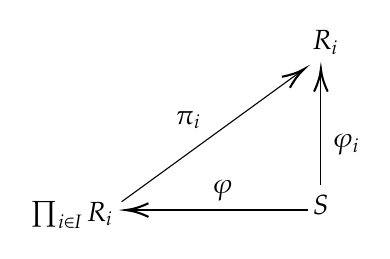
\begin{tikzpicture}[x=0.75pt,y=0.75pt,yscale=-1,xscale=1]
%uncomment if require: \path (0,476); %set diagram left start at 0, and has height of 476

%Straight Lines [id:da7996461945512099] 
\draw    (370,260) -- (284,260) ;
\draw [shift={(282,260)}, rotate = 360] [color={rgb, 255:red, 0; green, 0; blue, 0 }  ][line width=0.75]    (10.93,-3.29) .. controls (6.95,-1.4) and (3.31,-0.3) .. (0,0) .. controls (3.31,0.3) and (6.95,1.4) .. (10.93,3.29)   ;
%Straight Lines [id:da9398415640083908] 
\draw    (376,248) -- (376,194) ;
\draw [shift={(376,192)}, rotate = 90] [color={rgb, 255:red, 0; green, 0; blue, 0 }  ][line width=0.75]    (10.93,-3.29) .. controls (6.95,-1.4) and (3.31,-0.3) .. (0,0) .. controls (3.31,0.3) and (6.95,1.4) .. (10.93,3.29)   ;
%Straight Lines [id:da6839385952780701] 
\draw    (280,256) -- (366.38,193.18) ;
\draw [shift={(368,192)}, rotate = 143.97] [color={rgb, 255:red, 0; green, 0; blue, 0 }  ][line width=0.75]    (10.93,-3.29) .. controls (6.95,-1.4) and (3.31,-0.3) .. (0,0) .. controls (3.31,0.3) and (6.95,1.4) .. (10.93,3.29)   ;

% Text Node
\draw (371,251.4) node [anchor=north west][inner sep=0.75pt]    {$S$};
% Text Node
\draw (235,254.4) node [anchor=north west][inner sep=0.75pt]    {$\prod _{i\in I} R_{i}$};
% Text Node
\draw (323,244.4) node [anchor=north west][inner sep=0.75pt]    {$\varphi $};
% Text Node
\draw (371,172.4) node [anchor=north west][inner sep=0.75pt]    {$R_{i}$};
% Text Node
\draw (381,222.4) node [anchor=north west][inner sep=0.75pt]    {$\varphi _{i}$};
% Text Node
\draw (305,211.4) node [anchor=north west][inner sep=0.75pt]    {$\pi _{i}$};


\end{tikzpicture}
\end{center}
\end{note}
\begin{proof}
We have shown the existence of $\varphi$ in previous chapter. It is easy to verify that $\varphi$ is a homomorphism and therefore $\prod_{i\in I}R_i$ is the product in the category of rings and therefore determined up to isomorphism.
\end{proof}
\begin{theorem}
Let $A_1,A_2,\cdots,A_n$ be ideals in a ring $R$ such that $A_1+A_2+\cdots+A_n=R$ and for each $k$, $A_k\cap(A_1+\cdots+A_{k-1}+A_{k+1}+\cdots+A_n)=0$, then there is a ring isomorphism $R\cong A_1\times A_2\times\cdots\times A_n$.
\end{theorem}
\begin{proof}
By Theorem 2.66 we know that the map $\varphi:A_1\times A_2\times\cdots\times A_n\to R$ given by $(a_1,a_2,\cdots,a_n)\mapsto a_1+a_2+\cdots+a_n$ is an isomorphism of additive abelian groups. It suffices to show that $\varphi$ is a ring homomorphism, which we observe that 
$$
\left( a_1+a_2+\cdots +a_n \right) \left( b_1+b_2+\cdots +b_n \right) =a_1b_1+a_2b_2+\cdots +a_nb_n,
$$
since $a_ib_j\in A_i\cap A_j=0$, therefore $\varphi$ is a ring homomorphism and we finished our proof.
\end{proof}
If $R$ is a ring and $A_1,\cdots,A_n$ are ideals in $R$ that satisfy the hypothesis of Theorem 4.34, then $R$ is said to be the \textbf{(internal) direct product} of the ideals $A_i$. As groups, there are small differences between these two concepts in rings. For example, if a ring $R$ is the internal product of some ideals $A_1,\cdots,A_n$, then each of $A_i$ is actually an ideal contained in $R$ and $R$ is isomorphic to the external product $A_1\times\cdots\times A_n$. However, the external direct product does not contain the $A_i$, it simply contain the copies, say $\iota_i(A_i)$, of each $A_i$. These differences are unimportant in practise, so we often omit the adjective internal or external, and use the following notations: We write $R=\prod A_i$ or $R=A_1\times\cdots\times A_n$ to indicate that the ring $R$ is the internal direct product of its ideals $A_i$.\par
We close this section with a useful result. We first introduce some terminologies. Let $A$ be an ideal in a ring $R$ and $a,b\in R$. The element $a$ is said to be \textbf{congruent} to $b$ modulo $A$ (denoted $a\equiv b(\mathrm{mod}A)$) if $a-b\in A$. Since $R/A$ is a ring, $a_1\equiv a_2(\mathrm{mod}A)$ and $b_1\equiv b_2(\mathrm{mod}A)$ implies $a_1+b_1\equiv a_2+b_2(\mathrm{mod}A)$ and $a_1a_2\equiv b_1b_2(\mathrm{mod}A)$.
\begin{theorem}(Chinese Remainder Theorem)
Let $A_1,\cdots,A_n$ be ideals in a ring $R$ such that $R^2+A_i=R$ for all $i$ and $A_i+A_j=R$ for all $i\ne j$. If $b_1,\cdots,b_n\in R$, then there exists $b\in R$ such that $b\equiv b_i(\mathrm{mod}A_i)$ for all $i=1,2,\cdots,n$. Furthermore $b$ is uniquely determined up to congruence modulo the ideal $A_1\cap\cdots\cap A_n$.
\end{theorem}
\begin{proof}
Since $A_1+A_2=R$ and $A_1+A_3=R$, we have 
$$
R^2=\left( A_1+A_2 \right) \left( A_1+A_3 \right) =A_{1}^{2}+A_1A_3+A_2A_1+A_2A_3\subset A_1+\left( A_2\cap A_3 \right) .
$$
Therefore 
$$
R=A_1+R^2\subset A_1+\left( A_2\cap A_3 \right) \subset R,
$$
whence $R=A_1+(A_2\cap A_3)$. Now we show that $R=A_1+\bigcap_{i\ne 1}A_i$ inductively. Suppose $R=A_1+\left( A_2\cap A_3\cap \cdots \cap A_{k-1} \right) $, then we have 
$$
R^2=\left[ A_1+\left( A_2\cap A_3\cap \cdots \cap A_{k-1} \right) \right] \left( A_1+A_k \right) \subset A_1+\left( A_2\cap A_3\cap \cdots \cap A_k \right) \subset R,
$$
whence $R=A_1+(A_2\cap\cdots\cap A_k)$. Now that $R=A_1+\left( \bigcap_{i\ne 1}{A_i} \right) $ and analogously we may show that $R=A_k+\left( \bigcap_{i\ne k}{A_i} \right) $. Therefore for all $b_k\in R$, there exists $a_k\in A_k$ and $r_k\in\bigcap_{i\ne k}A_i$ such that $b_k=a_k+r_k$, whence $r_k\equiv b_k(\mathrm{mod}A_k)$ for all $k=1,2,\cdots,n$. Observe that $r_i\equiv0(\mathrm{A_j})$ when $i\ne j$, then let $b=r_1+r_2+\cdots+r_n$, we conclude that $b\equiv b_i(\mathrm{mod}A_i)$ for all $i=1,2,\cdots,n$. Now we show that $b$ is uniquely determined up to the congruence modulo $\bigcap A_i$. Suppose $c\equiv b_i(\mathrm{mod}A_i)$, then $b-c\in A_i$ for all $A_i$. Hence $b\equiv c\left( \mathrm{mod}\bigcap_{i=1}^n{A_i} \right) $, we finished our proof.
\end{proof}
The Chinese Remainder Theorem is so named because it is a generalization of the following fact from elementary number theory, which is known to the Chinese mathematicians in the first century A.D.
\begin{corollary}
Let $m_1,m_2,\cdots,m_n$ be positive integers such that $(m_i,m_j)=1$ for $i\ne j$. If $b_1,b_2,\cdots,b_n$ are any integers, then the system of congruences $x=b_i(\mathrm{mod}m_i)$ has an integral solution that is uniquely determined modulo $m=m_1m_2\cdots m_n$.
\end{corollary}
\begin{proof}
Let $A_i=(m_i)$. Clearly $\bigcap A_i=(m)$ and $(m_i,m_j)=1$ implies $A_i+A_j=\mathbb{Z}$. Then the result follows from the Chinese Remainder Theorem.
\end{proof}
\begin{corollary}
If $A_1,A_2,\cdots,A_n$ are ideals of $R$, then there exists a monomorphism of rings 
$$
\theta :R/\left( A_1\cap A_2\cap \cdots \cap A_n \right) \rightarrow R/A_1\times R/A_2\times \cdots \times R/A_n.
$$
If $R^2+A_i=R$ for all $i$ and $A_i+A_j=R$ for all $i\ne j$, then $\theta$ is an isomorphism of rings.
\end{corollary}
\begin{proof}
We first show that there is a monomorphism $\theta$. Define 
$$
\theta _1:R\rightarrow R/A_1\times R/A_2\times \cdots \times R/A_n
$$
given by $r\mapsto(r+A_1,\cdots,r+A_n)$. Clearly the kernel of $\theta_1$ is $\bigcap A_i$. Therefore by the First Isomorphism Theorem we have the monomorphism 
$$
\theta :R/\left( A_1\cap A_2\cap \cdots \cap A_n \right) \rightarrow R/A_1\times R/A_2\times \cdots \times R/A_n.
$$
Now we show that under the given condition $\theta$ is an isomorphism. In fact, let 
$$
\left( b_1+A_1,\cdots ,b_n+A_n \right) \in R/A_1\times R/A_2\times \cdots \times R/A_n,
$$
there exists $b\in R$ such that $b\equiv b_i(\mathrm{mod}A_i)$ for all $i=1,2,\cdots,n$. Hence 
$$
\theta \left( b+\bigcap{A_i} \right) =\left( b+A_1,\cdots ,b+A_n \right) =\left( b_1+A_1,\cdots ,b_n+A_n \right) ,
$$
and therefore $\theta$ is an epimorphism.
\end{proof}
\begin{center}
\begin{large}
    \textbf{Exercises for 4.2}
\end{large}
\end{center}
\begin{problem}\em
The set of all nilpotent elements in a commutative ring forms an ideal.
\end{problem}
\begin{proof}
Let $I=\{r\in R:r^n=0\ \text{for some}\ n\in\mathbb{N}\}$. Then let $r\in R$ and $i\in I$, we have $(ir)^n=i^nr^n=0$, hence $ir\in I$. Therefore $I$ is a right ideal of $R$. Similarly we may show that $I$ is a left ideal of $R$, and hence an ideal.
\end{proof}
\begin{problem}\em
Let $I$ be an ideal in a commutative ring $R$ and let $\mathrm{Rad}I=\{r\in R:r^n\in I\ \text{for some}\ n\in\mathbb{N}\}$. Show that $\mathrm{Rad}I$ is an ideal.
\end{problem}
\begin{proof}
Let $j\in\mathrm{Rad}I$ and $j^n=i\in I$. Suppose $r\in R$, then $(jr)^n=j^nr^n=ir^n\in I$, hence $jr\in\mathrm{Rad}I$, therefore $\mathrm{Rad}I$ is a right ideal of $R$. Similarly we may show that $\mathrm{Rad}I$ is a left ideal of $R$, and hence an ideal.
\end{proof}
\begin{problem}\em
If $R$ is a ring and $a\in R$, then $J=\{r\in R:ra=0\}$ is a left ideal and $K=\{r\in R:ar=0\}$ is a right ideal in $R$.
\end{problem}
\begin{proof}
We first show that $J$ is a left ideal of $R$. Let $j\in J$, then for all $r\in R$, we have $rj\in J$ since $rja=r(ja)=0$, and hence $J$ is a left ideal of $R$. Similarly we may prove that $K$ is a left ideal of $R$.
\end{proof}
\begin{problem}\em
If $I$ is a left ideal in a ring $R$, then $A(I)=\{r\in R:rx=0\ \text{for every}\ x\in I\}$ is an ideal in $R$.
\end{problem}
\begin{proof}
Let $a\in A(I)$. Then for all $r\in R$, we show that $ar\in A(I),ra\in A(I)$. First, $arx=ar^\prime=0$ since $I$ is a left ideal of $R$ implies $rx=r^\prime\in I$, then by the definition of $A(I)$ we conclude that $ar\in A(I)$. Then $rax=r0=0$ since $a\in A(I)$ and $x\in I$, therefore $A(I)$ is an ideal of $R$.
\end{proof}
\begin{problem}\em
If $I$ is an ideal in a ring $R$, let $[R:I]=\{r\in R:xr\in I\ \text{for all}\ x\in R\}$. Show that $[R:I]$ is an ideal which contains $I$.
\end{problem}
\begin{proof}
Let $a\in[R:I]$ and $r\in R$. Then $xar=\left( xa \right) r=ir\in I$, where $i\in I$ and by the fact that $I$ is an ideal we conclude that $ar\in[R:I]$. Also observe that $xra=(xr)a\in I$, we have $ra\in I$ and hence $[R:I]$ is an ideal of $R$. Clearly for all $i\in I$, we have $xi\in I$ for all $x\in R$, hence $I\subset[R:I]$.
\end{proof}
\begin{problem}\em
(a) The center of the ring $S$ of all $2\times 2$ matrices over a field $F$ consists of all matrices of the form $
\left( \begin{matrix}
	a&		0\\
	0&		a\\
\end{matrix} \right) 
$.\par
(b) The center of $S$ is not an ideal of $S$.\par
(c) What is the center of the ring of all $n\times n$ matrices over a division ring?
\end{problem}
\begin{proof}
(a) Observe that 
$$
\left\{ \begin{array}{c}
	\left( \begin{matrix}
	a&		b\\
	c&		d\\
\end{matrix} \right) \left( \begin{matrix}
	1&		0\\
	0&		0\\
\end{matrix} \right) =\left( \begin{matrix}
	a&		0\\
	c&		0\\
\end{matrix} \right) ,\\
	\left( \begin{matrix}
	1&		0\\
	0&		0\\
\end{matrix} \right) \left( \begin{matrix}
	a&		b\\
	c&		d\\
\end{matrix} \right) =\left( \begin{matrix}
	a&		b\\
	0&		0\\
\end{matrix} \right) ,\\
\end{array} \right. \Rightarrow b=c=0;\left\{ \begin{array}{c}
	\left( \begin{matrix}
	a&		b\\
	c&		d\\
\end{matrix} \right) \left( \begin{matrix}
	0&		1\\
	0&		0\\
\end{matrix} \right) =\left( \begin{matrix}
	0&		a\\
	0&		0\\
\end{matrix} \right) ,\\
	\left( \begin{matrix}
	0&		1\\
	0&		0\\
\end{matrix} \right) \left( \begin{matrix}
	a&		b\\
	c&		d\\
\end{matrix} \right) =\left( \begin{matrix}
	0&		d\\
	0&		0\\
\end{matrix} \right) ,\\
\end{array} \right. \Rightarrow a=d.
$$
Therefore elements in the center of $S$ must have the form $
\left( \begin{matrix}
	a&		0\\
	0&		a\\
\end{matrix} \right) 
$. Now we show that all matrices of the form $
\left( \begin{matrix}
	a&		0\\
	0&		a\\
\end{matrix} \right) 
$ is in the center of $S$. Observe that 
$$
\left( \begin{matrix}
	a&		0\\
	0&		a\\
\end{matrix} \right) \left( \begin{matrix}
	x&		y\\
	z&		w\\
\end{matrix} \right) =\left( \begin{matrix}
	x&		y\\
	z&		w\\
\end{matrix} \right) \left( \begin{matrix}
	a&		0\\
	0&		a\\
\end{matrix} \right) =\left( \begin{matrix}
	ax&		ay\\
	az&		aw\\
\end{matrix} \right) .
$$\par
(b) Let $C$ denote the center of $S$. Observe that 
$$
\left( \begin{matrix}
	a&		0\\
	0&		a\\
\end{matrix} \right) \left( \begin{matrix}
	1&		0\\
	0&		0\\
\end{matrix} \right) =\left( \begin{matrix}
	a&		0\\
	0&		0\\
\end{matrix} \right) \notin C,
$$
hence $C$ is not an ideal of $S$.\par
(c) Similar to (b) we may show that the center of all $n\times n$ matrices over a field consists of all elements $aE_n$, where $E_n=\mathrm{diag}\{1,\cdots,1\}$. Observe that $aE_n$ has an inverse $\frac{1}{a}E_n$, hence it is an element of all $n\times n$ matrices over a division ring. Therefore the center of which is $\{aE_n:a\in D\}$.
\end{proof}
\begin{problem}\em
(a) A ring $R$ with identity is a division ring if and only if $R$ has no proper left ideals.\par
(b) If $S$ is a ring with no proper left ideals, then either $S^2=0$ or $S$ is a division ring.
\end{problem}
\begin{proof}
(a) Let $R$ be a division ring. Then for all $S$ subring of $R$ that do not contain $1_R$, every $s\in S$ has an inverse $s^{-1}\in R$ such that $s^{-1}s=1_R\notin S$, hence $S$ is not an ideal of $R$. Therefore an ideal of $R$ must contain $1_R$, which is the trivial ideal of $R$. Conversely, suppose $R$ has only trivial ideal $R$, then for all $r\in R$, there exists some $s\in R$ such that $rs=1_R$, hence $R$ is a division ring.\par
(b) Suppose that $S^2\ne S$, we show that $S$ is a division ring, which suffices to show that $S$ has an identity. Consider $I=\{a\in S:Sa=0\}$, which is easily to be proved an ideal of $S$. Therefore $I=0$ or $I=S$. By the given condition we know that $I=0$, hence $Sa=0$ if and only if $a=0$. Therefore for each nonzero element $a\in S$, we have $Sa=S$, and this implies right cancellation, since $(x-y)s=0$ implies $x-y=0$, which is $x=y$ when $s$ is a nonzero element. Now $Sa=S$, hence there exists some $e\in S$ such that $ea=a$, and $e^2a=ea$. $a$ is a nonzero element, hence by the right cancellation we have $e^2=e$. Clearly $e\ne 0$, therefore $e$ is an identity element of $S$, whence $S$ is a division ring.
\end{proof}
\begin{problem}\em
Let $R$ be a ring with identity and $S$ the ring of all $n\times n$ matrices over $R$. $J$ is an ideal of $S$ if and only if $J$ is a ring of all $n\times n$ matrices over $I$ for some ideal $I$ in $R$.
\end{problem}
\begin{proof}
Let $J$ be an ideal of $S$, let $I$ be the set of all elements that appears in the matrices of $J$. To show that $I$ is an ideal of $R$, it suffices to show that for all $a\in I$ and $E_{ij}$, which denote the matrix with element $1_R$ at position $(i,j)$ and $0$ in other, $aE_{ij}\in J$. Now choose $B\in J$ such that $b_{st}=a$. Observe that 
$$
E_{is}BE_{tj}=\sum_{u,v}{b_{uv}E_{is}E_{uv}E_{tj}}=\sum_{u,v}{b_{uv}\delta _{su}\delta _{vt}E_{ij}}=aE_{ij}\in J,
$$
where $B=\sum_{u,v}b_{uv}E_{uv}\in J$ and $\delta_{ij}$ is the Kronecker symbol, we conclude that $I$ is an ideal of $R$.
\end{proof}
\begin{problem}\em
Let $S$ be the ring of all $n\times n$ matrices over a division ring $D$.\par
(a) $S$ has no proper ideals.\par
(b) $S$ has zero divisors. Consequently, $S\cong S/0$ is not a division ring and $0$ is a prime ideal.
\end{problem}
\begin{proof}
(a) Suppose $J$ is an ideal of $S$. Then by Exercise 4.25 we know that the elements of matrices in $J$ is an ideal of $D$, which is a division ring and has to be trivial. Therefore $J$ is the trivial ideal of $S$. which is not proper.\par
(b) Consider 
$$
\left( \begin{matrix}
	1&		&		&		\\
	&		1&		&		\\
	&		&		\ddots&		\\
	&		&		&		1\\
\end{matrix} \right) \left( \begin{matrix}
	&		&		&		1\\
	&		&		&		\\
	&		&		&		\\
	&		&		&		\\
\end{matrix} \right) =0\in S.
$$
Therefore $S$ has zero divisors and $S\cong S/0$ is not a division ring with $0$ is a prime ideal.
\end{proof}
\begin{note}\em
The example in this exercise does not satisfy condition given in Theorem 4.25.
\end{note}
\begin{problem}\em
(a) Show that $\mathbb{Z}$ is a principal ideal ring.\par
(b) Every homomorphic image of a principal ideal ring is also a principal ideal ring.\par
(c) $\mathbb{Z}_m$ is a principal ideal ring for every $m>0$.
\end{problem}
\begin{proof}
(a) Let $I$ be an ideal of $\mathbb{Z}$, then $I$ is a subring of $\mathbb{Z}$. By Theorem 2.15 we conclude that $I$ is of the form $m\mathbb{Z}$, where $m\in\mathbb{Z}$. Therefore $I=(m)$, which is a principal ideal. Since this is true for all ideals of $\mathbb{Z}$, we showed that $\mathbb{Z}$ is a principal ideal domain.\par
(b) Let $R$ be a principal ideal ring and $f:R\to S$ is a homomorphism. Suppose $S=\mathrm{Im}f$, we now show that $S$ is a principal ideal ring. Let $I=(m)$ is an ideal of $R$, that is, for all $r\in R$ we have $rI\subset I$. Therefore $f(rI)=f(r)f(I)\subset f(I)$ and hence $f(I)$ is an ideal of $S$. Since $I=(m)$, we have $f(I)=(f(m))$ by Theorem 4.15, therefore $f(I)$ is a principal ideal of $S$. Since this is true for all ideals of $S$, we conclude that $S$ is a principal ideal ring.\par
(c) This is a direct corollary of (b).
\end{proof}
\begin{problem}\em
If $N$ is the ideal of all nilpotent elements in a commutative ring $R$, then $R/N$ is a ring with no nonzero nilpotent elements.
\end{problem}
\begin{proof}
Suppose $r+N\in R/N$ and $(r+N)^n=r^n+N=r+N$. Then $r^n=r$, hence $r\in N$. Therefore $R/N$ has no nonzero nilpotent elements.
\end{proof}
\begin{problem}\em
Let $R$ be a ring without identity and with no zero divisors. Let $S$ be the ring whose additive group is $R\times\mathbb{Z}$ as in the proof of Theorem 4.10. Let $A:\{(r,n)\in S:rx+nx=0\ \text{for every}\ x\in R\}$.\par
(a) $A$ is an ideal in $S$.\par
(b) $S/A$ has an identity and contains a subring isomorphic to $R$.\par
(c) $S/A$ has no zero divisors.
\end{problem}
\begin{proof}
(a) This is easy to verify through definition.\par
(b) Let $a\in A$, then clearly $aA$ is an identity of $S/A$. Now we define $f:S\to R$ given by $(a,b)\mapsto a$, which is an epimorphism. Therefore by the First Isomorphism Theorem $f$ induces an epimorphism $\overline{f}:S/A\to R$, which implies that $S/A$ has an subring isomorphic to $R$.\par
(c) If not, then there exists some $(r,n)(s,m)\in A$ and $(r,n),(s,m)\notin A$. Therefore $(rs+mr+ns,nm)\in A$, whence for all $x\in S$, we have 
$$(rs+mr+ns)x+(nm)x=rsx+mrx+nsx+nmx=0.$$
Since $(s,m)\notin A$, we have $sx+mx\ne 0$ for some $x\in R$. Denote $sx+mx=t$. Now it suffices to show that $rx+nx=0$ for all $x\in R$. Now observe that 
$$rt+nt=0\Leftrightarrow t(rt+nt)=0\Leftrightarrow trt+nt^2=0\Leftrightarrow (tr+nt)t=0\Leftrightarrow tr+nt=0,$$
then we may conclude that 
$$tr+nt=0\Leftrightarrow trx+ntx=0\Leftrightarrow t(rx+nx)=0\Leftrightarrow rx+nx=0,$$
which finished the proof.
\end{proof}
\begin{problem}\em
Let $f:R\to S$ be a homomorphism of rings, $I$ an ideal in $R$, and $J$ an ideal in $S$.\par
(a) $f^{-1}(J)$ is an ideal in $R$ that contains $\mathrm{Ker}f$.\par
(b) If $f$ is an epimorphism, then $f(I)$ is an ideal in $S$. If $f$ is not surjective, $f(I)$ need not be an ideal in $S$.
\end{problem}
\begin{proof}
(a) Since the kernel is the smallest ideal of $R$, it suffices to show that $f^{-1}(J)$ is an ideal. Let $r\in R$. Then there exists some $s\in S$ such that $f^{-1}(s)=r$. Therefore $rf^{-1}(J)=f^{-1}(x)f^{-1}(J)=f^{-1}(xJ)\subset f^{-1}(J)$, whence $f^{-1}(J)$ is a right ideal of $R$. This is true for left ideal, hence $f^{-1}(J)$ is an ideal of $R$.\par
(b) Let $s\in S$. Since $f$ is an epimorphism, we have $f(r)=s$ for some $r\in R$. Therefore $sf(I)=f(r)f(I)=f(rI)\subset f(I)$, hence $f(I)$ is a right ideal of $S$. This is also true for left ideal, hence $f(I)$ is an ideal of $S$. Now consider the injective homomorphism $f:\mathbb{Z}\to\mathbb{Q}$, clearly $2\mathbb{Z}$ is an ideal of $\mathbb{Z}$, but $f(2\mathbb{Z})=2\mathbb{Z}$ is not an ideal of $\mathbb{Q}$.
\end{proof}
\begin{problem}\em
If $P$ is an ideal in a not necessarily commutative ring $R$, then the following conditions are equivalent.\par
(a) $P$ is a prime ideal.\par
(b) If $r,s\in R$ are such that $rRs\subset P$, then $r\in P$ or $s\in P$.\par
(c) If $(r)$ and $(s)$ are principal ideals of $R$ such that $(r)(s)\subset P$, then $r\in P$ or $s\in P$.\par
(d) If $U$ and $V$ are right ideals such that $UV\subset P$, then $U\subset P$ or $V\subset P$.\par
(e) If $U$ and $V$ are left ideals such that $UV\subset P$, then $U\subset P$ or $V\subset P$.
\end{problem}
\begin{proof}
We first show that (a), (b) and (c) are equivalent.\par
(a)$\Rightarrow$(b): Suppose $P$ is a prime ideal, then if $(RrR)(RsR)\subset P$, we have $(RrR)\subset P$ or $(RsR)\subset P$. Say $(RrR)\subset P$. Observe that $RrR$ is an ideal of $R$, hence $(RrR)=RrR$. Now consider $(r)=A$, since $A^3\subset RrR\subset P$ we have $(r)^3\subset P$, whence $r\in A\subset P$. Hence $r\in P$.\par
(a)$\Rightarrow$(c): This is trivial.\par
(c)$\Rightarrow$(b): Since $(r)$ is an ideal of $R$, then $(r)R(s)\subset P$, whence $rRs\subset P$. Then by (b) we conclude that $r\in P$ or $s\in P$.\par
(b)$\Rightarrow$(a): Suppose $A,B$ are ideals of $P$ such that $AB\subset P$, but neither $A\subset P$ nor $B\subset P$. Then let $a\in P\setminus A$ and $b\in P\setminus B$, we have $aRb\subset P$, a contradiction!\par
Now we show that (a), (d) and (e) are equivalent. Since the proof of right ideals are analogous to that of left ideals, we only show (a) and (d) are equivalent.\par
(a)$\Rightarrow$(d): Let $A,B$ be left ideals of $R$ such that $AB\subset P$ and $A\not\subset P$. Then there exists some $a\in A\setminus P$ such that $aB\subset P$, whence $ab\in P$ for all $b\in B$. This shows $b\in P$ by the property of a prime ideal, and hence $B\subset P$ since this is true for all $b\in B$.\par
(d)$\Rightarrow$(a): Trivial.
\end{proof}
\begin{problem}\em
The set consisting of zero and all zero divisors in a commutative ring with identity contains at least one prime ideal.
\end{problem}
\begin{proof}
We introduce a Theorem that will be proved in commutative algebra:\par
\textbf{Theorem}: If $S$ is a multiplicative subset of a ring $R$ which is disjoint from an ideal $I$ of $R$, then there exists an ideal $P$ which is maximal in the set of all ideals of $R$ disjoint from $S$ and containing $I$. Furthermore, $P$ is prime.\par
Now let $Z=\{a\in R:a\ne0,ab\ne 0\ \text{for all}\ 0\ne b\in R\}$. Consider $S=R-Z$. By the theorem above it suffices to show that $S$ is multiplicative. Let $ab\in S$. By the definition of $S$ we have $a,b$ are both not zero divisors. Now suppose $ab$ is a zero divisor, then there exists some $c\in R$ such that $c(ab)=0$. Since $R$ is commutative, we have $a(cb)=0$, which contradict to the fact that $b$ is not a zero divisor, hence $S$ is multiplicative and we finished our proof.
\end{proof}
\begin{problem}\em
Let $R$ be a commutative ring with identity and suppose that the ideal $A$ of $R$ is contained in a finite union of prime ideals $P_1\cup P_2\cup\cdots\cup P_n$. Show that $A\subset P_i$ for some $i$.
\end{problem}
\begin{proof}
We prove by contradiction. Suppose $A\not\subset P_i$ for all $i\in\{1,2,\cdots,n\}$, then $A\cap P_i\cap\left(\bigcap_{j\ne i}P_j\right)\ne\emptyset$ for all $i\in\{1,2,\cdots,n\}$. Now choose $a_i\in(A\cap P_i)\setminus\left(\bigcup_{j\ne i}P_j\right)$, we have $a_1+a_2a_3\cdots a_n\in A$, but not in $\bigcup_{i=1}^nP_i$, a contradiction!
\end{proof}
\begin{problem}\em
Let $f:R\to S$ be an epimorphism of rings with kernel $K$.\par
(a) If $P$ is a prime ideal in $R$ that contains $K$, then $f(P)$ is a prime ideal in $S$.\par
(b) If $Q$ is a prime ideal in $S$, then $f^{-1}(Q)$ is a prime ideal in $R$ that contains $K$.\par
(c) There is a one-to-one correspondence between the set of all prime ideals in $R$ that contains $K$ and the set of all prime ideals in $S$, given by $P\mapsto f(P)$.\par
(d) If $I$ is an ideal in a ring $R$, then every prime ideal in $R/I$ is of the form $P/I$, where $P$ is a prime ideal in $R$ that contains $I$.
\end{problem}
\begin{proof}
(a) Clearly $f(P)$ is an ideal of $S$, it suffices to show that $f(P)$ is a prime ideal of $S$. The epimorphism $f:R\to S$ induces an isomorphism $\overline{f}:R/K\to S$, hence it suffices to show that $P/K$ is a prime ideal of $R/K$. Let $(A/K)(B/K)\subset P/K$, then $AB/K\subset P/K$, whence $AB+K\subset P+K$, which is $AB\subset P$. Since $P$ is a prime ideal of $R$, we have $A\subset P$ or $B\subset P$, hence $P/K$ is a prime ideal of $S$ and we finished our proof.\par
(b) The proof of which is similar to (a).\par
(c) Since $f:R\to S$ induces an isomorphism $\overline{f}:R/K\to S$, and if $P$ is an ideal of $R$, we have $P/K$ is an ideal of $S$, hence we have the one-to-one correspondence $P\mapsto f(P)$ of prime ideals of $R$ and prime ideals of $S$.\par
(d) Observe that the ideal of $R/I$ is of the form $J/I$, where $J$ is an ideal of $R$, therefore $P/I$ is an ideal of $R/I$ when $P$ is a prime ideal of $R$. Then consider the canonical injection $\pi:R\to R/I$, we have $\pi^{-1}(P/I)=P$, then by (b) we conclude that the prime ideal of $R/I$ is of the form $P/I$.
\end{proof}
\begin{problem}\em
An ideal $M\ne R$ in a commutative ring $R$ with identity is maximal if and only if for every $r\in R-M$, there exists $x\in R$ such that $1_R-rx\in M$.
\end{problem}
\begin{proof}
Suppose $M$ is maximal. Then for $r\in R-M$, consider the ideal $(M,r)$. Since $M$ is maximal and $(M,r)\supset M$, we conclude that $(M,r)=R$ for $M$ is the maximal ideal of $R$. Since $R$ is a commutative ring, we have $m+rx\in R$. In particular, $1_R\in R$ and hence $m+rx=1_R$ for some $x\in R$. Conversely, we show that $R/M$ is a division ring. Clearly $1_RM$ is the identity of $R/M$. Now it suffices to show that each $r+M\in R/M$ is a unit. This follows by the fact that $rx\equiv 1_R(\mathrm{mod}M)$ for some $x$ and hence we finished our proof.
\end{proof}
\begin{problem}\em
The ring $E$ of even integers contains a maximal ideal $M$ such that $E/M$ is not a field.
\end{problem}
\begin{proof}
Consider $M=(4)$, which we now show is a maximal ideal of $E$. Clearly $M$ is an ideal of $E$. Suppose $I$ is another ideal of $E$ and $M\subset I\subset E$, we have $4k+2\in I$ or otherwise $I\subset M$. Therefore $(M,2)\subset I$ and $(M,2)=E$, which implies that $M$ is the maximal ideal of $E$. However $E/M$ has no identity. The only two elements of $E/M$ are $\overline{2}$ or $\overline{4}$. However $\overline{2}\times\overline{2}=\overline{4}\times\overline{2}=\overline{4}$, which shows that $E/M$ has no identity element.
\end{proof}
\begin{problem}\em
In the ring $\mathbb{Z}$ the following conditions on a nonzero ideal $I$ are equivalent:\par
(i) $I$ prime; (ii) $I$ is maximal; (iii) $I=(p)$ with $p$ prime.
\end{problem}
\begin{proof}
(i)$\Rightarrow$(ii): Suppose $I$ is a prime ideal. Since $\mathbb{Z}$ is principal ideal domain, we suppose $I=(p)$. Suppose $ab\subset (p)$, then $p\mid ab$. Since $I$ is a prime ideal, we have $p\mid a$ or $p\mid b$. Therefore $p$ is prime. Now suppose $J$ is another ideal contains $I$, then $J=(1)$ since $I$ is prime, hence $J=\mathbb{Z}$ and $I$ is maximal.\par
(ii)$\Rightarrow$(iii): Suppose $I=(p)$ and $p$ is not prime, then there exists some prime $p_1$ such that $p=kp_1$. Consider $(p_1)$, which is an ideal that contains $I$ but not equal to $\mathbb{Z}$, which contradict to the fact that $I$ is maximal. Hence $p$ is prime.\par
(iii)$\Rightarrow$(i): Suppose $ab\in (p)$. Since $p$ is prime, we have $p\mid a$ or $p\mid b$, therefore $a\in (p)$ or $b\in (p)$. Therefore $(p)$ is prime.
\end{proof}
\begin{problem}\em
Determine all prime and maximal ideals in the ring $\mathbb{Z}_m$.
\end{problem}
\begin{proof}
Since $\mathbb{Z}_m=\mathbb{Z}/m\mathbb{Z}$, by Exercise 4.34(d) we know that the prime ideals of $\mathbb{Z}_m$ are of the form $p\mathbb{Z}/m\mathbb{Z}$, where $p\mid m$. The maximal ideals of $\mathbb{Z}_m$ are precisely the prime ideals.
\end{proof}
\begin{problem}\em
If $R_1,\cdots,R_n$ are rings with identity and $I$ is an ideal in $R_1\times R_2\times\cdots\times R_n$, then $I=A_1\times A_2\times\cdots\times A_m$, where $A_i$ is an ideal in $R_i$.\par
\end{problem}
\begin{proof}
Consider the canonical epimorphism $\pi_k:R_1\times R_2\times\cdots\times R_n\to R_k$, then let $A_k=\pi_k(I)$, we have $A_k$ an ideal of $R_k$ and $I=A_1\times A_2\times\cdots\times A_n$.\par
\end{proof}
\begin{note}\em
Note that the conclusion may be false if the rings $R_i$ does not have identities.
\end{note}
\begin{problem}\em
An element $e$ in a ring $R$ is said to be \textbf{idempotent} if $e^2=e$. An element of the center of the ring $R$ is said to be \textbf{central}. If $e$ is a central idempotent in a ring $R$ with identity, then\par
(a) $1_R-e$ is a central idempotent;\par
(b) $eR$ and $(1_R-e)R$ are ideals in $R$ such that $R=eR\times(1_R-e)R$.
\end{problem}
\begin{proof}
(a) First we observe that 
$$
\left( 1_R-e \right) ^2=\left( 1_R-e \right) \left( 1_R-e \right) =1_R-e-e+e^2=1_R-e,
$$
hence $1_R-e$ is a idempotent element. Also observe that 
$$
\left( 1_R-e \right) r=r-er=r-re=r\left( 1_R-e \right) ,
$$
we conclude that $1_R-e$ is a central idempotent.\par
(b) We first show that $eR$ is an ideal of $R$. Let $er\in eR$, then $r^\prime er=er^\prime r\in eR$, hence $eR$ is an ideal of $R$. Also we may verify that $(1_R-e)R$ is an ideal of $R$. Now that $er+(1_R-e)r=er+r-er=r\in R$, hence $R=eR\times(1_R-e)R$.
\end{proof}
\begin{problem}\em
Idempotent elements $e_1,\cdots,e_n\in R$ are said to be \textbf{orthogonal} if $e_ie_j=0$ for $i\ne j$. If $R_1,\cdots,R_n$ are rings with identity, then the following conditions are equivalent:\par
(a) $R\cong R_1\times R_2\times\cdots\times R_n$;\par
(b) $R$ contains a set of orthogonal central idempotents $\{e_1,\cdots,e_n\}$ such that $e_1+\cdots+e_n=1_R$ and $e_iR\cong R_i$ for each $i$.\par
(c) $R$ is the internal direct product $R=A_1\times A_2\times\cdots\times A_n$, where $A_i$ is an ideal of $R$ such that $A_i\cong R_i$.
\end{problem}
\begin{proof}
(a)$\Rightarrow$(b): Let $\overline{e_i}=(0,\cdots,1_R,\cdots,0)$, then $\overline{e_i}\in R_1\times R_2\times\cdots\times R_n$, and $\sum\overline{e_i}=1_R$. Clearly $\{\overline{e_1},\cdots,\overline{e_n}\}$ are orthogonal and $\overline{e_i}R\cong R_i$.\par
(b)$\Rightarrow$(c): Let $A_k=e_kR$, observe that $A_k$ is then the principal ideal $(e_k)$ of $R$ and $A_k$ itself is a ring with identity $e_k$.\par
(c)$\Rightarrow$(a): Trivial.
\end{proof}
\begin{problem}\em
If $m\in\mathbb{Z}$ has a prime decomposition $m=p_1^{k_1}\cdots p_t^{k_t}$ where $k_i>0$ and $p_i$ are primes, then there is an isomorphism of rings $\mathbb{Z}_m\cong\mathbb{Z}_{p_1^{k_1}}\times\cdots\times\mathbb{Z}_{p_t^{k_t}}$.
\end{problem}
\begin{proof}
We first show that $\mathbb{Z}^2+p_i^{k_i}\mathbb{Z}=\mathbb{Z}$ for all $i$. This is trivial since for all $m\in\mathbb{Z}$, we have $(m-p_i^{k_i})+p_i^{k_i}=m$. Now we show that $p_i^{k_i}\mathbb{Z}+p_j^{k_j}\mathbb{Z}=\mathbb{Z}$. Since $(p_i^{k_i},p_j^{k_j})=1$, by Bezout's Theorem we have $mp_i^{k_i}+np_j^{k_j}=1$. Hence for all $r\in\mathbb{Z}$ we have $rmp_i^{k_i}+rnp_j^{k_j}=r$. Now by Corollary 4.37 we have
$$
\theta :\mathbb{Z} /\left( p_{1}^{k_1}\mathbb{Z} \cap \cdots \cap p_{t}^{k_t}\mathbb{Z} \right) \rightarrow \mathbb{Z} /p_{1}^{k_1}\mathbb{Z} \times \cdots \times \mathbb{Z} /p_{t}^{k_t}\mathbb{Z} 
$$
is an isomorphism. Hence
$$
\mathbb{Z} _m=\mathbb{Z} /m\mathbb{Z} \cong \mathbb{Z} /\left( p_{1}^{k_1}\mathbb{Z} \cap \cdots \cap p_{t}^{k_t}\mathbb{Z} \right) \cong \mathbb{Z} /p_{1}^{k_1}\mathbb{Z} \times \cdots \times \mathbb{Z} /p_{t}^{k_t}\mathbb{Z} =\mathbb{Z} _{p_{1}^{k_1}}\times \cdots \times \mathbb{Z} _{p_{t}^{k_t}}.
$$
\end{proof}
\subsection{Factorization in Commutative Rings}
In this section, we shall extend the concept of divisibility, greatest common divisor and prime in the ring of integers to arbitrary commutative rings and study those integral domains in which an analogue of the Fundamental Theorem of Arithmetic holds. The chief result is that every PID is UFD. In addition we study those commutative rings in which an analogue of the division algorithm is valid(Euclidean rings).
\begin{definition}
A nonzero element $a$ of a commutative ring $R$ is said to be \textbf{divide} an element $b\in R$, if there exists $x\in R$ such that $ax=b$. Elements $a,b\in R$ are said to be \textbf{associates} if $a\mid b$ and $b\mid a$.
\end{definition}
Virtually all statements about divisibility may be phrased in terms of principal ideals as we shall see.
\begin{theorem}
Let $a,b$ and $u$ be elements of a commutative ring $R$ with identity.\par
(i) $a\mid b$ if and only if $(b)\subset (a)$.\par
(ii) $a$ and $b$ are associates if and only if $(a)=(b)$.\par
(iii) $u$ is a unit if and only if $u\mid r$ for all $r\in R$.\par
(iv) $u$ is a unit if and only if $(u)=R$.\par
(v) The relation "$a$ is associates with $b$" is an equivalence relation on $R$.\par
(vi) If $a=br$ with $r\in R$ a unit, then $a$ and $b$ are associates. If $R$ is an integral domain, the converse id true.
\end{theorem}
\begin{proof}
(i) Suppose $a\mid b$, then $b=ax$ for some $x\in R$. Therefore we have $\left( b \right) =bR=axR\subset aR=\left( a \right) $ and hence $(b)\subset(a)$. Conversely, if $(b)\subset (a)$, then $bR\subset aR$ and hence there exists some $x\in R$ such that $b=ax$. Therefore $a\mid b$.\par
(ii) If $a$ and $b$ associates, we have $a\mid b$ and $b\mid a$. Hence $(a)\subset (b)\subset (a)$ and therefore $(a)=(b)$. Conversely, if $(a)=(b)$, then $(a)\subset (b)$ and $(b)\subset (a)$. Therefore $a\mid b$ and $b\mid a$, whence $a$ and $b$ are associates.\par
(iii) Suppose $u$ is a unit, then there exists some $v\in R$ such that $uv=1_R$. Now for all $r\in R$, we have $rv\in R$ such that $urv=r$, therefore $u\mid r$. Conversely, suppose $u\mid r$ for all $r\in R$, let $r=1_R$, we have $uv=1_R$ for some $v\in R$, therefore $u$ is a unit.\par
(iv) Let $u$ be a unit, then $u\mid 1_R$. Hence $(1_R)\subset (u)$. However $(1_R)=R$, hence $(u)=R$. Conversely, if $(u)=R$, then for all $r\in R$, there exists $v\in R$ such that $uv=r$, therefore $u$ is a unit.\par
(v) Verify by definition.\par
(vi) Since $a=br$, we have $b\mid a$. However $u$ is a unit, therefore there exists some $v\in R$ such that $av=b$, whence $a\mid b$. Hence $a$ and $b$ associates. Conversely, suppose $R$ is an integral domain, then we have $u,v\in R$ such that $a=bu$ and $b=av$. Therefore $a=avu$. Since $R$ is an integral domain, we have $vu=1_R$, hence $u$ is a unit.
\end{proof}
\begin{definition}
Let $R$ be a commutative ring with identity. An element $c$ of $R$ is \textbf{irreducible} provided that:\par
(i) $c$ is a nonzero nonunit;\par
(ii) $c=ab$ implies $a$ or $b$ is a unit.\par
An element $p$ of $R$ is \textbf{prime} provided that:\par
(i) $p$ is a nonzero nonunit;\par
(ii) $p\mid ab$ implies $p\mid a$ and $p\mid b$.
\end{definition}
Here are some examples.
\begin{example}\em
If $p$ is a prime number in $\mathbb{Z}$, then both $p$ and $-p$ are irreducible and prime in $\mathbb{Z}$. In the ring $\mathbb{Z}_6$, $\overline{2}$ is prime but not irreducible, since $\overline{2}=\overline{2}\cdot\overline{4}$, however both $\overline{2}$ and $\overline{4}$ are zero divisors. We will give an example of an irreducible element which is not prime in exercises.
\end{example}
There is a close connection between prime [resp. irreducible] elements in a ring $R$ and prime [resp. maximal] ideals in $R$.
\begin{theorem}
Let $p$ and $c$ be nonzero elements in an integral domain $R$.\par
(i) $p$ is prime if and only if $(p)$ is nonzero prime ideal.\par
(ii) $c$ is irreducible if and only if $(c)$ is maximal in the set $S$ of all proper principal ideals of $R$.\par
(iii) Every prime element of $R$ is irreducible.\par
(iv) If $R$ is a PID, then $p$ is prime if and only if $p$ is irreducible.\par
(v) Every associate of an irreducible [resp. prime] element of $R$ is irreducible [resp. prime].\par
(vi) The only divisors of an irreducible element of $R$ are its associates and the units in $R$.
\end{theorem}
\begin{note}\em
Several parts of Theorem 4.41 are true for any commutative ring with identity as we will see in the following proof.
\end{note}
\begin{proof}
(i) Suppose $p$ is prime. Then $p\mid ab$ implies $p\mid a$ or $p\mid b$. Therefore if $ab\in (p)$, we have $a\in (p)$ or $b\in (p)$, whence $(p)$ is a prime ideal. Conversely, since $R$ is an integral domain, therefore $R$ is commutative and apply Theorem 4.25 we conclude that $p$ is prime.\par
(ii) Suppose $c$ is irreducible. Then suppose $(c)\subset(d)\subset R$, we have $d\mid c$ and hence $c=dx$ for some $x\in R$. Since $c$ is irreducible, we have $d$ is a unit or $x$ is a unit. If $d$ is a unit, then $(d)=R$. If $x$ is a unit, then $(d)=(c)$, whence $(c)$ is the maximal ideal of all proper ideals of $R$. Conversely, suppose $(c)$ is the maximal ideal of all proper principal ideals of $R$. Then suppose $c=ab$, we have $(c)\subset(a)\subset R$. If $(a)=R$, then $a$ is a unit. Otherwise $cy=a$, whence $cyb=ab=c$ and hence $yb=1_R$ since $R$ is an integral domain. Therefore $b$ is a unit and hence $c$ is an irreducible element.\par
(iii) Let $p=ab$, then $p\mid a$ or $p\mid b$. We may assume that $p\mid a$. Therefore $a=px$ for some $x\in R$. Therefore $p=ab=pxb$. Since $R$ is an integral domain, we have $xb=1_R$ and hence $b$ is a unit. Therefore $p$ is a irreducible element.\par
(iv) We have shown that every prime element of $R$ is an irreducible element, now we show that converse. Since $R$ is PID, then $(p)$ is the maximal ideal of $R$. However for PID the maximal ideal is prime, hence $p$ is prime.\par
(v) We only prove the condition of irreducible elements, and the condition of prime elements are similar. Suppose $c$ is irreducible and $d$ associates with $c$, then $(c)=(d)$. Hence $(d)$ is a maximal ideal of all principal ideals of $R$, whence $d$ is an irreducible element.\par
(vi) Let $c\in R$ be an irreducible element and $d\mid c$. Then $(c)\subset (d)$, whence $(c)=(d)$ or $(c)=R$. If $(c)=(d)$, then $c$ associates with $d$, if $(c)=R$, then $c$ is a unit.
\end{proof}
We have now developed some analogues in an arbitrary integral domain of the concepts of divisibility and prime numbers in the ring $\mathbb{Z}$. Recall that every element in $\mathbb{Z}$ is a product of a finite number of irreducible elements according to the Fundamental Theorem of Arithmetic, we introduce the concept of UFD:
\begin{definition}
An integral domain $R$ is a \textbf{unique factorization domain} provided that:\par
(i) every nonzero element $a\in R$ can be written $a=c_1c_2\cdots c_n$ with $c_i\in R$ irreducible;\par
(ii) If $a=c_1c_2\cdots c_n$ and $a=d_1d_2\cdots d_m$ with $c_i$ and $d_j$ irreducible, then $m=n$ and for some permutation $\sigma$ of $\{1,2,\cdots,n\}$, $c_i$ and $d_{\sigma(i)}$ are associates for every $i$.
\end{definition}
\begin{note}\em
From (ii) we know that every irreducible element of a UFD is prime. Suppose $R$ is UFD and $p\in R$ is irreducible, then $p\mid ab$ implies $ab=cp$ for some $c\in R$. Suppose $a=a_1\cdots a_m$, $b=b_1\cdots b_n$ and $c=c_1\cdots c_r$, then $a_1\cdots a_nb_1\cdots b_m=pc_1\cdots c_r$, whence $p$ is associates to some $a_i$ or $b_j$, hence $p\mid a$ or $p\mid b$, therefore $p$ is prime.
\end{note}
Now we give an important theorem. To prove it, we need the following lemma:
\begin{lemma}\em
Let $R$ be a PID and $(a_1)\subset(a_2)\subset\cdots\subset(a_n)\subset\cdots$ is a chain of ideals of $R$, then the ascending terminates for some $n$, i.e., $(a_j)=(a_n)$ for some $n$ and all $j\ge n$.
\end{lemma}
\begin{proof}
Let $A=\bigcap_{i\ge 1}(a_i)$, we show that $A$ is an ideal. Let $a,b\in A$, whence $a\in (a_i)$ and $b\in (a_j)$ for some $i,j$. Suppose $i\ge j$, then $(a_j)\subset(a_i)$, and $a,b\in (a_i)$. Since $(a_i)$ is an ideal, we have $a-b\in (a_i)$, hence $a-b\in A$. Also we may show that for $r\in R$ and $a\in A$, we have $ra\in A$, therefore by Theorem 4.12 we have $A$ is an ideal. Since $R$ is a PID, we have $A=(a)$. Since $a\in\bigcup_{i\ge 1}(a_i)$, there are some $(a_n)$ such that $a\in (a_n)$, therefore $(a)\subset (a_n)$. However $(a)\subset (a_n)\subset (a_j)\subset A$, we have $(a_n)=(a_j)$ for all $j\ge n$.
\end{proof}
Now we give the following theorem:
\begin{theorem}
Every PID is a UFD.
\end{theorem}
\begin{proof}
Suppose $S$ be the set of all elements of $R$ that are nonzero and nonunit, and cannot be factored into a finite product of some irreducible elements. We first show that $S=\emptyset$, such that every nonzero and nonunit element in $R$ can be factorized into some product of irreducible elements.\par
Suppose $a\in S$. Then $(a)$ is a proper ideal contained in $R$, and therefore, since $R$ has an identity, we have $(a)$ is contained in some maximal ideal of $R$, say $(c_a)$. Therefore $c_a\mid a$ and hence for each $a\in S$, there exists some (which requires the Axiom of Choice) $x_a$ such that $a=c_ax_a$. Also note that $x_a$ here is unique since $R$ is an integral domain, and thus the cancellation holds. We show that $x_a\in S$. If not, then either $x_a$ is a unit or $x_a$ can be factorized. If $x_a$ is a unit, then $(x_a)=R$. However $x_a\mid a$, hence $(a)\subset(x_a)$ and therefore $a$ is a unit, a contradiction! If $x_a$ can be factorized, then $a=c_ax_a$ can be factorized, a contradiction! Therefore $x_a\in S$.\par
Now we show that $(a)$ is properly contained in $(x_a)$. First, $(a)\subset(x_a)$ since $x_a\mid a$, now suppose $(a)=(x_a)$, then $x_a=ay$ for some $y\in R$. Hence $a=x_ac_a=ayc_a$, whence $yc_a=1_R$, which contradict to the fact that $c_a$ is irreducible for $(c_a)$ is maximal ideal.\par
Now we define $f:S\to S$ given by $a\mapsto x_a$. Then by Recursion Theorem there exists some $\varphi:\mathbb{N}\to S$ such that $\varphi(0)=a$ and $\varphi(n+1)=f(\varphi(n))$. Therefore by defining $\varphi(n)=a_n$, we get a sequence $\{a_n\}_{n\ge 1}$ subset of $S$. However by the preceding discussion we have the ascending ideal chain:
$$
\left( a \right) \underset{\ne}{\subset}\left( a_1 \right) \underset{\ne}{\subset}\left( a_2 \right) \underset{\ne}{\subset}\cdots \underset{\ne}{\subset}\left( a_n \right) \underset{\ne}{\subset}\cdots ,
$$
which contradict to Lemma 4.1! Hence $S$ is empty.\par
Now we show that the factorization is unique. Suppose $a=c_1c_2\cdots c_n=d_1d_2\cdots d_m$, where $c_i$ and $d_j$ are irreducible for $1\le i\le n$ and $1\le j\le m$. Since $c_1$ is irreducible and $R$ is a PID, $c_1$ is prime and hence $c_1\mid d_j$ for some $j$. Since $c_1$ is not a unit, then it must associate with some $d_j$. Then by induction we finished our proof.
\end{proof}
\begin{note}\em
The converse of Theorem 4.43 is false. For example, the polynomial ring $\mathbb{Z}[x]$ can be shown to be a UFD, but $\mathbb{Z}[x]$ is not a PID.
\end{note}
Several important integral domains that we shall meet frequently have certain properties not shared by all integral domains.
\begin{definition}
Let $\mathbb{N}$ be the set of all nonnegative integers and $R$ is a commutative ring. $R$ is a \textbf{Euclidean ring} if there is a function $\varphi:R\setminus\{0\}\to\mathbb{N}$ such that: \par
(i) if $a,b\in R$ and $ab\ne 0$, then $\varphi(a)\Leftrightarrow\varphi(ab)$;\par
(ii) if $a,b\in R$ and $b\ne 0$, then there exist $q,r\in R$ such that $a=qb+r$ with $r=0$, or $r\ne 0$ and $\varphi(r)<\varphi(b)$.\par
A Euclidean ring which is an integral domain is called an \textbf{Euclidean domain}.
\end{definition}
We give some examples of EDs (Euclidean Domains).
\begin{example}\em
(i) The ring $\mathbb{Z}$ is an ED. Define $\varphi:x\mapsto|x|$.\par
(ii) If $F$ is a field, then $F$ is an ED. Define $\varphi:x\mapsto 1$.\par
(iii) If $F$ is a field, then consider the ring of polynomials $F[x]$. If we define $\varphi(f)=\mathrm{deg}f$, then $F[x]$ is an ED.\par
(iv) Consider \textbf{the domain of Gauss integers} $\mathbb{Z}[i]$, which contains all the complex numbers of the form $a+bi$, where $a,b\in\mathbb{Z}$. Define $\varphi(a+bi)=a^2+b^2$, then $\mathbb{Z}[i]$ is an ED.
\end{example}
\begin{theorem}
Every Euclidean ring $R$ is a principal ideal ring with identity. Consequently every ED is a UFD.
\end{theorem}
\begin{proof}
Let $R$ be an Euclidean ring and $I$ is an ideal of $R$. Then for some $a\in I$, we have $(a)\subset I$. Let $b$ be the infimum of the set $\{\varphi(x):x\ne 0\}$. Suppose $a=bq+r$ for some $r=0$ or $\varphi(r)<\varphi(b)$. If $r\ne 0$, then $\varphi(r)<\varphi(b)$, a contradiction! Hence $r=0$ and $a=bq$. Therefore $I\subset Ra\subset(a)\subset I$ and hence $I=(a)$. Since $R$ is an ideal of $R$, we have $rR\subset R$ for some $r\in R$. Therefore there exists some $e\in R$ such that $r=er=re$, whence $e$ is the identity of $R$. Now if $R$ is an integral domain, we have $R$ a PID.
\end{proof}
\begin{note}\em
The converse of this theorem is false. Consider $\mathbb{Z}\left[\frac{1+\sqrt{-19}}{2}\right]$, which is a PID but not an ED.
\end{note}
We close this section with some further observations on divisibility that will be used occasionally in the sequel.
\begin{definition}
Let $X$ be a nonempty subset of a commutative ring $R$. An element $d\in R$ is a \textbf{greatest common divisor} of $X$ provided:\par
(i) $d\mid a$ for all $a\in X$;\par
(ii) $c\mid a$ for all $a\in X$ implies $c\mid d$.
\end{definition}
\begin{note}\em
The common divisors does not always exist. For example, in the ring of all even numbers $E$, $2$ has no divisors, hence $2$ and $4$ has no greatest common divisors. In a commutative ring with identity, if the greatest common divisor of $a_1,a_2,\cdots,a_n$ is $1_R$, then we say $a_1,a_2,\cdots,a_n$ are \textbf{relatively prime}.
\end{note}
\begin{theorem}
Let $a_1,a_2,\cdots,a_n$ be elements of a commutative ring $R$ with identity.\par
(i) $d\in R$ is a greatest common divisor of $\{a_1,a_2,\cdots,a_n\}$ such that $d=r_1a_1+r_2a_2+\cdots+r_na_n$ for some $r_i\in R$ if and only if $(d)=(a_1)+(a_2)+\cdots+(a_n)$.\par
(ii) If $R$ is a PID, then a greatest common divisor of $a_1,a_2,\cdots,a_n$ exists and every one is of the form $r_1a_1+r_2a_2+\cdots+r_na_n$.\par
(iii) If $R$ is UFD, then there exists a greatest common divisor of $a_1,a_2,\cdots,a_n$.
\end{theorem}
\begin{proof}
(i) Since $R$ is a commutative ring with identity, we have $\left( a_i \right) =\left\{ \sum{r_ja_i}:r_j\in R \right\} $. Now if $d$ is a greatest common divisor of $a_1,a_2,\cdots,a_n$ and $d=r_1a_1+r_2a_2+\cdots+r_na_n$, then $(d)=(a_1)+(a_2)+\cdots+(a_n)$. Conversely, if $(d)=(a_1)+(a_2)+\cdots+(a_n)$, then 
$$
\left( d \right) =\sum_i{\left\{ \sum_j{r_ja_i}:r_j\in R \right\}}=\left\{ \sum_j{r_j\left( \sum_i{a_i} \right)}:r_j\in R \right\} =\left( \sum_i{a_i} \right) =\sum_i{\left( a_i \right)}.
$$\par
(ii) Since $R$ is PID, then the ideal $(a_1)+(a_2)+\cdots+(a_n)$ is still an ideal, and it is a principal ideal, denote as $(d)$. Then by (i) we conclude that $d$ is the common divisor of $a_1,a_2,\cdots,a_n$.\par
(iii) Since $R$ is UFD, we may assume $a_i=c_{1}^{m_{i1}}c_{2}^{m_{i2}}\cdots c_{t}^{m_{it}}$, where $c_i$ is irreducible. Then consider $d=c_{1}^{k_1}c_{2}^{k_2}\cdots c_{t}^{k_t}$, where $k_j=\min \left\{ m_{1j},m_{2j},\cdots ,m_{nj} \right\} $, one may verify that $d$ is the largest common divisor of $a_1,a_2,\cdots,a_n$.
\end{proof}
\begin{note}\em
Note that the Theorem does not state that every greatest common divisor of $a_1,a_2,\cdots,a_n$ can be expressed into the linear combination of $a_1,a_2,\cdots,a_n$.
\end{note}
\begin{center}
\begin{large}
    \textbf{Exercises for 4.3}
\end{large}
\end{center}
\begin{problem}\em
A nonzero ideal in a principal ideal domain is maximal if and only if it is prime.
\end{problem}
\begin{proof}
Suppose $R$ is a PID and $p$ is a prime element in $R$. Then $p$ is irreducible. Since $p$ prime implies $(p)$ prime and $p$ irreducible implies $(p)$ maximal, we conclude that every prime ideal is maximal in PID.
\end{proof}
\begin{problem}\em
An integral domain $R$ is UFD id and only if every nonzero prime ideal of $R$ contains a nonzero principal ideal that is prime.
\end{problem}
\begin{proof}
This is a theorem of Kaplansky's. We show only one direction. Suppose $R$ is UFD and $I$ is a prime ideal of $R$. If $a\in I$, then $a=a_1a_2\cdots a_n$. Since $I$ is a prime ideal, we have $a_j\in I$ for some $j$. Therefore $(a_j)$ is a desired principal ideal.\par
The converse is much more complex and requires some techniques of commutative algebra, we skip the proof.
\end{proof}
\begin{problem}\em
Let $R$ be the subring $\mathbb{Z}[\sqrt{10}]$ of the field of real numbers.\par
(a) The mapping $N:R\to\mathbb{Z}$ given by $a+b\sqrt{10}\mapsto(a+b\sqrt{10})(a-b\sqrt{10})$ is such that $N(uv)=N(u)N(v)$ for all $u,v\in R$ and $N(u)=0$ if and only if $u=0$.\par
(b) $u$ is a unit in $R$ is and only if $N(u)=\pm1$.\par
(c) $2,3,4+\sqrt{10}$ and $4-\sqrt{10}$ are irreducible elements in $R$, but not prime elements in $R$.
\end{problem}
\begin{proof}
(a) It is easy to verify that $N(uv)=N(u)N(v)$ for all $u,v\in R$. Now if $N(u)=0$, suppose $u=a+b\sqrt{10}$, then $N(u)=a^2-10b^2=0$, whence $a=\pm\sqrt{10}b$. If $a=b\sqrt{10}$, then $a+b\sqrt{10}=2b\sqrt{10}$, whence $N(u)=-40b^2=0$ and $b=0$, therefore $a=b=0$. If $a=-b\sqrt{10}$, then $u=0$.\par
(b) Suppose $N(u)=1$, then let $\overline{u}=\frac{N(u)}{u}$, hence $N(u)=u\overline{u}$. Now that $N(u)=1$, we conclude that $\overline{u}$ is an inverse element of $u$. Conversely, if $u$ is a unit, then there exists some $v$ such that $uv=1$, hence $N(uv)=N(u)N(v)=1$. Since $N(u)$ and $N(v)$ are both integers, we have $N(u)=1$ or $N(u)=-1$.\par
(c) We only show that $2$ is irreducible, the others may be showed analogously. Suppose $2=(a+b\sqrt{10})(c+d\sqrt{10})$, then $2=(a-b\sqrt{10})(c-d\sqrt{10})$, whence $4=(a^2-10b^2)(c^2-10d^2)$. By modulo $16$ one may omit the condition of $a^2-10d^2=\pm2$, hence there exists $a+b\sqrt{10}$ or $c+d\sqrt{10}$ that is a unit. However, observe that $2\mid 10=\sqrt{10}\cdot\sqrt{10}$, but $2\nmid\sqrt{10}$, hence $2$ is not prime.
\end{proof}
\begin{note}\em
Note that $6=2\cdot 3=(4+\sqrt{10})(4-\sqrt{10})$, hence $\mathbb{Z}[\sqrt{10}]$ is not a UFD.
\end{note}
\begin{problem}\em
Show that the integral domain of Exercise 4.45 every element can be factored into a product of irreducibles, but the factorization need not be unique.
\end{problem}
\begin{proof}
It suffices to show that the existence of the factorization. We do it by induction. If $N(a)=2$, then the condition is trivial. Now suppose this is true for all $N(b)\ge 2$. Consider $2\le N(b)<N(a)$. If $a$ is irreducible, then we are done. Otherwise $a=b_1b_2$ with $2\le N(b_i)<N(a)$, then by the induction hypothesis we have $b_i$ are irreducible, which finished the proof.
\end{proof}
\begin{problem}\em
Let $R$ be a PID.\par
(a) Every proper ideal is a product $P_1,P_2,\cdots,P_n$ of maximal ideals, which are uniquely determined up to order.\par
(b) An ideal $P$ in $R$ is said to be \textbf{primary} if $ab\in P$ and $a\notin P$ imply $b^n\in P$ for some $n$. Show that $P$ is primary if and only if for some $n$, $P=(p^n)$, where $p\in R$ is prime or $p=0$.\par
(c) If $P_1,P_2,\cdots,P_n$ are primary ideals such that $P_i=(p_i^{n_i})$ and the $p_i$ are primes, then $P_1P_2\cdots P_n=P_1\cap P_2\cap\cdots\cap P_n$.\par
(d) Every proper ideal in $R$ can be expressed (uniquely up to order) as the intersection of a finite number of primary ideals.
\end{problem}
\begin{proof}
(a) Note that in a commutative ring we have $(a)(b)=(ab)$, hence for a PID, consider any ideal $(r)$ of $R$. Since every PID is a UFD, we have $r=a_1a_2\cdots a_n$, which is determined uniquely up to order. Therefore $(r)=(a_1a_2\cdots a_n)=(a_1)(a_2)\cdots(a_n)$.\par
(b) Suppose $P=(p^n)$ for some prime $p$. Then suppose $ab\in P$ and $a\notin P$, then $ab=kp^n$ and $a\ne lp^n$. Therefore $b=rp^i$ for some $i$. Consider $b^n=r^np^{ni}$, we have $b^n\in P$. Conversely, suppose $P=(x)$ with $x=p_{1}^{\alpha _1}p_{2}^{\alpha _2}\cdots p_{n}^{\alpha _n}$. Then let $a=p_1^{\alpha_1}$ and $b=p_2^{\alpha_2}\cdots p_n^{\alpha_n}$, if $a\in P$, then $P=(p_1^{n\alpha_i})$ for some $n$. Otherwise $b^n\in P$, hence 
$$
p_{1}^{\alpha _1}p_{2}^{\alpha _2}\cdots p_{n}^{\alpha _n}\mid p_{2}^{n\alpha _2}\cdots p_{n}^{n\alpha _n}\Rightarrow p_{1}^{\alpha _1}\mid p_{2}^{\left( n-1 \right) \alpha _2}\cdots p_{n}^{\left( n-1 \right) \alpha _n}\Rightarrow p_1\mid p_j,j\in \left\{ 2,3,\cdots ,n \right\} ,
$$
a contradiction unless $n=1$ or $P=(0)$.\par
(c) It suffices to show that $P_1P_2=P_1\cap P_2$ and by induction we get the desired conclusion. Suppose $x\in P_1P_2$, then $x=\sum a_kb_k$, where $a_k\in P_1$ and $b_k\in P_2$. Therefore $x\in P_1\cap P_2$ and hence $P_1P_2\subset P_1\cap P_2$. For the reverse inclusion, we consider $x\in P_1\cap P_2$, therefore $x=a_0p_1^{n_1}=b_0p_2^{n_2}$, and hence $p_2\mid a_0p_1^{n_1}$. This implies $p_2\mid a_0$ since $p_2\mid p_1^{n_1}$ leads to contradiction. Now we have $a_0=a_1p_2$ for some $a_1\in R$ and hence $x=a_1p_2p_1^{n_1}=b_0p_2^{n_2}$. Since $R$ is a PID, we may cancel $p_2$ and hence $a_1p_1^{a_1}=b_0p_2^{n_2-1}$. By induction one may show that $a_{n_2}p_1^{n_1}=b_0$ and hence $x=a_{n_2}p_1^{n_1}p_2^{n_2}$, whence $x\in P_1P_2$.\par
(d) Since $R$ is PID, hence $R$ is UFD. Therefore for a proper ideal $(x)$ in $R$, we have $x=p_{1}^{\alpha _1}p_{2}^{\alpha _2}\cdots p_{n}^{\alpha _n}$. Therefore we have 
$$
\left( x \right) =\left( p_{1}^{\alpha _1}p_{2}^{\alpha _2}\cdots p_{n}^{\alpha _n} \right) =\left( p_{1}^{\alpha _1} \right) \left( p_{2}^{\alpha _2} \right) \cdots \left( p_{n}^{\alpha _n} \right) ,
$$
and by (c) we have 
$$
\left( x \right) =\left( p_{1}^{\alpha _1} \right) \cap \left( p_{2}^{\alpha _2} \right) \cap \cdots \cap \left( p_{n}^{\alpha _n} \right) .
$$
\end{proof}
\begin{problem}\em
(a) If $a$ and $n$ are integers, $n>0$, then there exists integers $q$ and $r$ such that $a=qn+r$, where $|r|\le\frac{n}{2}$.\par
(b) The Gaussian integers $\mathbb{Z}[i]$ form a Euclidean domain with $\varphi(a+bi)=a^2+b^2$.
\end{problem}
\begin{proof}
(a) Define $q=\max \left\{ q_0:a\le q_0n \right\} $. If $qn=a$, then $r=0$, and the proof is finished. Otherwise let $r=a-qn$. If $|r|\le\frac{n}{2}$ the proof is also finished. For $|r|>\frac{n}{2}$, consider $r=a-(q+1)n$, then $|r|\le\frac{n}{2}$ and hence we finished our proof.\par
(b) Let $x\in\mathbb{Z}[i]\setminus\{0\}$. Therefore by the definition of $\mathbb{Z}[i]$ we have $|x|\ge 1$, whence $\varphi(a)\le\varphi(ab)$. To prove the rest part, consider $y=a+bi$, where $a,b\in\mathbb{Z}$ and assume $x$ is a positive integer. By (a) we have $a=q_1x+r_1$ and $b=q_2x+r_2$, where $|r_1|\le\frac{x}{2}$, $|r_2|\le\frac{x}{2}$. Now let $q=q_1x+r_1$ and $r=r_1x+r_2$, we have $y=qx+r$ with $r=0$ or $\varphi(r)<\varphi(x)$. In the general case, let $x=c+di$. Consider $\overline{x}=c-di$, $x\overline{x}>0$. There are $q_0,r_0\in\mathbb{Z}[i]$ such that $y\overline{x}=q(x\overline{x})+r_0$, with $r_0=0$ or $\varphi(r_0)<\varphi(x\overline{x})$. Let $r=y-qx$, then $y=qx+r$ and $r=0$ or $\varphi(r)<\varphi(x)$.
\end{proof}
\begin{problem}\em
What are the units in $\mathbb{Z}[i]$?
\end{problem}
\begin{proof}
Suppose $x=a+bi\in\mathbb{Z}[i]$ and $xy=1$. Let $y=c+di$, then we have 
$$
\begin{cases}
	ac-bd=1,\\
	ad+bc=0,\\
\end{cases}\Rightarrow \left\{ \begin{array}{c}
	c=\frac{-a}{a^2+b^2},\\
	d=\frac{-b}{a^2+b^2}\\
\end{array} \right. 
$$
however since $y\in\mathbb{Z}[i]$, we have $c,d\in\mathbb{Z}$, therefore there are only four units in $\mathbb{Z}[i]$: $1,-1,i,-i$.
\end{proof}
\begin{problem}\em
Let $R$ be a UFD and $d$ be a nonzero element of $R$. There are only a finite number of distinct principal ideals that contain in the ideal $(d)$.
\end{problem}
\begin{proof}
Suppose $(d)\subset (c)$, then since $R$ is a UFD we have $c\mid d$. Let $d=a_1a_2\cdots a_n$, we claim that $c$ is of the form $\prod a_i$ for some $i$. Otherwise since $d=kc$ for some $k\in R$ and the factorization is unique, we have $kc=a_1a_2\cdots a_n$, therefore $c=1$. Hence there are only $n!$ number of possible $c$'s that satisfies the condition.
\end{proof}
\begin{problem}\em
If $R$ is a UFD, $a,b\in R$ are relatively prime and $a\mid bc$, then $a\mid c$.
\end{problem}
\begin{proof}
Since $R$ is a UFD, we suppose 
$$
a=a_1a_2\cdots a_r,\hspace{0.5cm}b=b_1b_2\cdots b_s,\hspace{0.5cm}c=c_1c_2\cdots c_t.
$$
Since $a$ and $b$ are relatively prime, we know that for all $1\le i\le r$ and $1\le j\le s$, we have $a_i\nmid b_j$. Therefore by the fact that 
$$
a_1a_2\cdots a_r\mid b_1b_2\cdots b_sc_1c_2\cdots c_t,
$$
it has to be $a_i\mid c_k$ for some $1\le i\le r$ and $1\le k\le t$, whence $a\mid c$.
\end{proof}
\begin{problem}\em
Let $R$ be a Euclidean ring and $a\in R$. Then $a$ is a unit in $R$ if and only if $\varphi(a)=\varphi(1_R)$.
\end{problem}
\begin{proof}
Let $a$ be a unit. Then there exists some $b\in R$ such that $ab=1_R$. Observe that 
$$
\varphi \left( 1 \right) \le \varphi \left( 1\cdot a \right) =\varphi \left( a \right) \le \varphi \left( a\cdot b \right) \le \varphi \left( 1 \right) ,
$$
we have $\varphi(1)=\varphi(a)$. Conversely, suppose $\varphi(a)=\varphi(1)$, we show that $a$ is a unit. Suppose $1_R=qa+r$, where $r=0$ or $\varphi(r)<\varphi(a)$. However $\varphi(a)=\varphi(1_R)\le\varphi(r)$, we conclude that $r=0$ and hence $1_R=qa$, whence $a$ is a unit.
\end{proof}
\begin{problem}\em
Every nonempty set of elements (possibly infinite) in a commutative principal ideal ring with identity has a greatest common divisor.
\end{problem}
\begin{proof}
Since $R$ is PID, then the ideal $(a_1)+(a_2)+\cdots+(a_n)$ is still an ideal, and it is a principal ideal, denote as $(d)$. Then by Theorem 4.47(i) we conclude that $d$ is the common divisor of $a_1,a_2,\cdots,a_n$.
\end{proof}
\subsection{Rings of Quotients and Localization}
In the first part of this section the familiar construction of the field of rational numbers from the ring of integers is considerably generalized. The rings of quotients so constructed from any commutative ring are characterized by a universal property. The last part of this section deals with the prime ideal structure of rings of quotients and introduces localization at a prime ideal.\par
\begin{definition}
A nonempty subset $S$ of a ring $R$ is called \textbf{multiplicative} provided that $a,b\in S$ implies $ab\in S$.
\end{definition}
Here are some examples.
\begin{example}\em
The set $S$ of all elements in a nonzero ring with identity that are not zero divisors is multiplicative. In particular, the set of all nonzero elements in an integral domain is multiplicative. The set of all units in any ring with identity is multiplicative, If $P$ is a prime ideal in a commutative ring $R$, then both $P$ and $S=R-P$ are multiplicative.
\end{example}
The motivation for what follows may be seen most easily from the ring $\mathbb{Z}$ of integers and the field $\mathbb{Q}$ of rationals. The set $S=\mathbb{Z}\setminus\{0\}$ is clearly multiplicative in $\mathbb{Z}$, and the field $\mathbb{Q}$ is thought of as consisting of all fractions $a/b$ with $a\in\mathbb{Z}$ and $b\in S$, subject to the requirement 
$$
\frac{a}{b}=\frac{c}{d}\Leftrightarrow ad=bc.
$$
More precisely, $\mathbb{Q}$ may be constructed as follows. The relation on the set $\mathbb{Z}\times S$ defined by 
$$
\left( a,b \right) \sim \left( c,d \right) \Leftrightarrow ad-bc=0
$$
is easily seen as an equivalence relation. $\mathbb{Q}$ is defined to be the set of all equivalence class of $\mathbb{Z}\times S$ under this equivalence relation. The equivalence class of $(a,b)$ is denoted as $a/b$ and addition and multiplication is defined in the usual way.\par
We shall now extend our construction to any arbitrary multiplicative subset of any commutative ring $R$ (possibly without identity). We shall construct a commutative ring $S^{-1}R$ with identity and a homomorphism $\varphi_S:R\to S^{-1}R$. If $S$ is the set of all nonzero elements in an integral domain $R$, then $S^{-1}R$ will be a field ($S^{-1}R=\mathbb{Q}$ if $R=\mathbb{Z}$) and $\varphi_S$ will be a monomorphism embedding $R$ in $S^{-1}R$.
\begin{theorem}
Let $S$ be a multiplicative subset of a commutative ring $R$. The relation defined on the set $R\times S$ by $(r,s)\sim(r^\prime,s^\prime)\Leftrightarrow s_1(rs^\prime-r^\prime s)=0$ for some $s_i\in S$ is an equivalence relation. Furthermore if $R$ has no zero divisors and $0\notin S$, then $(r,s)\sim(r^\prime,s^\prime)\sim rs^\prime-r^\prime s=0$.
\end{theorem}
\begin{proof}
We first show that the first relation is an equivalence relation. First we observe that $(r,s)\sim(r,s)$ since for all $s_1\in S$ we have $s_1(rs-rs)=0$. Also note that if $(r,s)\sim(r^\prime,s^\prime)$, then for some $s_1\in S$ we have $s_1(rs^\prime-r^\prime s)=0$, therefore $s_1(r^\prime s-rs^\prime)=0$, whence $(r^\prime,s^\prime)\sim(r,s)$. Lastly, if $(r_1,s_1)\sim(r_2,s_2)$ and $(r_2,s_2)\sim(r_3,s_3)$, then we show that 
$$
\left( r_1,s_1 \right) \sim \left( r_2,s_2 \right) ,\left( r_2,s_2 \right) \sim \left( r_3,s_3 \right) \Rightarrow \left( r_1,s_1 \right) \sim \left( r_3,s_3 \right) 
$$
By definition of the relation we have $k_1r_1s_2=k_1r_2s_1,k_2r_2s_3=k_2r_3s_2$, therefore 
$$
k_1s_2k_2\left( r_1s_3-s_1r_3 \right) =k_1k_2r_1s_2s_3-k_1k_2s_1s_2r_3=k_1k_2r_3s_1s_2-k_1k_2s_1s_2r_3=0,
$$
which finished the proof. The second statement of the theorem is trivial since $R$ has no zero divisors.
\end{proof}
Let $S$ be a multiplicative subset of a commutative ring $R$ and $\sim$ the equivalence relation of Theorem 4.49. The equivalence class of $(r,s)\in R\times S$ is denoted as $r/s$. The set of all equivalence classes of $R\times S$ with $\sim$ will be denoted as $S^{-1}R$. Here are some trivial observations (which we omit the proof):\par
(i) $r/s=r^\prime/s^\prime$ if and only if $s_1(rs^\prime-r^\prime s)=0$ for some $s_1\in S$;\par
(ii) $tr/rs=r/s$ for all $r\in R$ and $s\in S$;\par
(iii) If $0\in S$, then $S^{-1}R$ consists of only one equivalence class.
\begin{theorem}
Let $S$ be the multiplicative subset of commutative ring $R$ and let $S^{-1}R$ be the set of equivalence classes of $R\times S$ under the equivalence relation of Theorem 4.49.\par
(i) $S^{-1}R$ is a commutative ring with identity, where addition and multiplication is defined as follows:
$$
r/s+r^{\prime}/s^{\prime}=\left( rs^{\prime}+r^{\prime}s \right) /ss^{\prime},\left( r/s \right) \left( r^{\prime}/s^{\prime} \right) =rr^{\prime}/ss^{\prime}.
$$\par
(ii) If $R$ is a nonzero ring with no zero divisors and $0\notin S$, then $S^{-1}R$ is an integral domain.\par
(iii) If $R$ is a nonzero ring with no zero divisors and $S$ is the set of all nonzero elements of $R$, then $S^{-1}R$ is a field.
\end{theorem}
\begin{proof}
(i) We first show that the addition and multiplication is well-defined. We consider $r/s=r^\prime/s^\prime$ and $r_1/s_1=r_1^\prime/s_1^\prime$. Therefore there exists some $s_2$ and $s_3$ such that 
$$
s_2\left( rs_1-r_1s \right) =s_3\left( r^{\prime}s_{1}^{\prime}-r_{1}^{\prime}s^{\prime} \right) =0.
$$
Therefore we have 
$$
s_2s_3\left[ \left( rs^{\prime}+r^{\prime}s \right) s_1s_{1}^{\prime}-\left( r_1s_{1}^{\prime}+r_{1}^{\prime}s_1 \right) ss^{\prime} \right] =0.
$$
Therefore $(rs^\prime+r^\prime s)s_1s_1^\prime=(r_1s_1^\prime+r_1^\prime s_1)/ss^\prime$. Similarly we may show that the multiplication is well-defined. Clearly $0/s$ is additive identity and additive inverse of $r/s$ is $-r/s$. For any $s\in S$, $s/s$ is the multiplicative identity.\par
(ii) Since $R$ is a nonzero ring with no zero divisors, we have $r/s=0/s$ if and only if $r=0$. Therefore $(r/s)(r^\prime/s^\prime)=0\in S^{-1}R$ if and only if $rr^\prime=0$, whence $r=0$ or $r^\prime=0$, whence $S^{-1}R$ is an integral domain.\par
(iii) Observe that for all $r/s\in S^{-1}R$, we have its inverse $s/r\in S^{-1}R$.
\end{proof}
The ring $S^{-1}R$ in Theorem 4.50 is called the \textbf{ring of quotients} or \textbf{ring of fractions} or \textbf{quotient ring} of $R$ by $S$. An important case of occurs when $R$ is an integral domain and $S$ is the set of all elements of $R$ without $0$, where $S^{-1}R$ is a field and we call it \textbf{quotient field of the integral domain} $R$. In particular, if $R=\mathbb{Z}$ then $S^{-1}R=\mathbb{Q}$. More generally suppose $R$ is any nonzero commutative ring and $S$ is the set of all nonzero elements that are not zero divisors, then $S^{-1}R$ is called the \textbf{complete ring of quotients} or \textbf{full ring of quotients} of the ring $R$. Therefore (iii) of Theorem 4.50 may be rephrased into the following: If $R$ is a nonzero ring with no zero divisors, then the complete ring of quotients $R$ is a field. Clearly every complete ring of quotients of any integral domain is just its quotient field.\par
If $\varphi:\mathbb{Z}\to\mathbb{Q}$ is the mapping defined by $n\mapsto n/1$, then clearly $\varphi$ is a monomorphism. More generally, we have the following theorem:
\begin{theorem}
Let $S$ be a multiplicative subset of the commutative ring $R$.\par
(i) The map $\varphi_S:R\to S^{-1}R$ given by $r\mapsto rs/s$ is a well-defined homomorphism of rings such that $\varphi_S(s)$ is a unit in $S^{-1}R$ for every $s\in S$.\par
(ii) If $0\notin S$ and $S$ contains no zero divisors, then $\varphi_S$ is a monomorphism. In particular, any integral domain can be embedded in its quotient field.\par
(iii) If $R$ has an identity and $S$ consists of units, then $\varphi_S$ is an isomorphism. In particular, the complete ring of quotients of a field $F$ is isomorphic to $F$.
\end{theorem}
\begin{proof}
(i) Suppose $s,s^\prime\in S$, then $rs/s=rs^\prime/s^\prime$, whence $\varphi_S$ is well-defined. Now we show that $\varphi_S$ is a homomorphism. By definition of $\varphi_S$ we have 
$$
\varphi _S\left( rs \right) =rss^{\prime}/s^{\prime}=\left( rs^{\prime}/s^{\prime} \right) \left( ss^{\prime}/s^{\prime} \right) =\varphi _S\left( r \right) \varphi _S\left( s \right) ,\hspace{0.5cm}r,s\in R.
$$
Observe that for each $\varphi_S(s)=ss^\prime/s^\prime$, we have $\varphi_S(s)\cdot(s^\prime/ss^\prime)=1_R$, hence $\varphi_S(s)$ is a unit in $S^{-1}R$.\par
(ii) Observe that 
$$
\varphi _S\left( r \right) =\varphi _S\left( s \right) \Rightarrow rs^{\prime}/s^{\prime}=ss^{\prime}/s^{\prime}\Rightarrow \left( r-s \right) s^{\prime\prime}s^{\prime}s^{\prime}=0\Rightarrow r=s,
$$
the last arrow holds since $R$ has no zero divisors, therefore $\varphi_S$ is a monomorphism.\par
(iii) By (ii) we know that $\varphi_S$ is a monomorphism. Now we show that $\varphi_S$ is an epimorphism under the condition of the theorem. Since $S$ consists of units, for a given $r/s$, consider $\varphi_S(rs^{-1})$.
\end{proof}
In view of Theorem 4.51(ii), we may identify an integral domain as a subring of its quotient field. Since $1_R\in S$ in this case, $r\in R$ is thus identified as $r/1_R\in R$.\par
The next theorem shows that rings of quotients may be completely characterized 
by a universal mapping property. This theorem is sometimes used as a definition of 
the ring of quotients.
\begin{theorem}
Let $S$ be a multiplicative subset of a commutative ring $R$ and let $T$ be any commutative ring with identity. If $f:R\to T$ is a homomorphism or rings such that $f(r)$ is a unit in $T$ for all $s\in S$, then there exists a unique $\overline{f}:S^{-1}R\to T$ such that $\overline{f}\varphi_S=f$. The ring $S^{-1}R$ is completely determined up to isomorphism with this property.
\end{theorem}
\begin{proof}
We first show the existence of such $\overline{f}$. Define $\overline{f}:r/s\mapsto f(r)[f(s)]^{-1}$, then 
$$
\overline{f}\circ \varphi _S\left( r \right) =\overline{f}\left( rs/s \right) =f\left( rs \right) \left[ f\left( s \right) \right] ^{-1}=f\left( r \right) f\left( s \right) \left[ f\left( s \right) \right] ^{-1}=f\left( r \right) .
$$
Now we show that such $\overline{f}$ is unique. Suppose there is another $g:S^{-1}R\to T$ such that $\varphi_S\circ g=f$, then by Exercise 4.14 we have $g([\varphi_S(s)]^{-1})=[g(\varphi_S(s)]^{-1}$ for all $s\in S$. Therefore 
$$
g\left( r/s \right) =g\left( \varphi _S\left( r \right) \left[ \varphi _S\left( s \right) \right] ^{-1} \right) =g\circ \varphi _S\left( r \right) \cdot \left[ g\circ \varphi _S\left( s \right) \right] ^{-1}=f\left( r \right) \left[ f\left( s \right) \right] ^{-1}=\overline{f}\left( r/s \right) 
$$
for all $r/s\in S^{-1}R$. Therefore $\overline{f}=g$.\par
To proof the rest part of this theorem, see Theorem 2.61.
\end{proof}
\begin{note}\em
In the language of Categories, we may rephrase this Theorem into the following commutative diagram: 
\begin{center}


\tikzset{every picture/.style={line width=0.75pt}} %set default line width to 0.75pt        

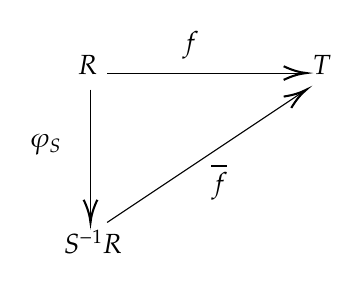
\begin{tikzpicture}[x=0.75pt,y=0.75pt,yscale=-1,xscale=1]
%uncomment if require: \path (0,476); %set diagram left start at 0, and has height of 476

%Straight Lines [id:da3152671411941921] 
\draw    (240,128) -- (334,128) ;
\draw [shift={(336,128)}, rotate = 180] [color={rgb, 255:red, 0; green, 0; blue, 0 }  ][line width=0.75]    (10.93,-3.29) .. controls (6.95,-1.4) and (3.31,-0.3) .. (0,0) .. controls (3.31,0.3) and (6.95,1.4) .. (10.93,3.29)   ;
%Straight Lines [id:da5751301154780408] 
\draw    (232,136) -- (232,198) ;
\draw [shift={(232,200)}, rotate = 270] [color={rgb, 255:red, 0; green, 0; blue, 0 }  ][line width=0.75]    (10.93,-3.29) .. controls (6.95,-1.4) and (3.31,-0.3) .. (0,0) .. controls (3.31,0.3) and (6.95,1.4) .. (10.93,3.29)   ;
%Straight Lines [id:da5543492055231241] 
\draw    (240,200) -- (334.34,137.11) ;
\draw [shift={(336,136)}, rotate = 146.31] [color={rgb, 255:red, 0; green, 0; blue, 0 }  ][line width=0.75]    (10.93,-3.29) .. controls (6.95,-1.4) and (3.31,-0.3) .. (0,0) .. controls (3.31,0.3) and (6.95,1.4) .. (10.93,3.29)   ;

% Text Node
\draw (225,118.4) node [anchor=north west][inner sep=0.75pt]    {$R$};
% Text Node
\draw (338,118.4) node [anchor=north west][inner sep=0.75pt]    {$T$};
% Text Node
\draw (202,156.4) node [anchor=north west][inner sep=0.75pt]    {$\varphi _{S}$};
% Text Node
\draw (218,202.4) node [anchor=north west][inner sep=0.75pt]    {$S^{-1} R$};
% Text Node
\draw (289,170.4) node [anchor=north west][inner sep=0.75pt]    {$\overline{f}$};
% Text Node
\draw (275,106.4) node [anchor=north west][inner sep=0.75pt]    {$f$};


\end{tikzpicture}
\end{center}
\end{note}
\begin{corollary}
Let $R$ be an integral domain considered as a subring of its quotient field $F$. If $E$ is a field and $f:R\to E$ is a monomorphism of rings, then there is a unique monomorphism of fields $\overline{f}:F\to E$ such that $\overline{f}\mid_R=f$. In particular any field $E_1$ containing $R$ contains an isomorphic copy $F_1$ of $F$ with $R\subset F_1\subset E$.
\end{corollary}
\begin{proof}
Let $S$ be the set of all nonzero elements of $R$ and apply Theorem 4.52 to $f:R\to E$. Then there is a homomorphism $\overline{f}:S^{-1}R\to E$ such that $\overline{f}\varphi_S=f$. To show that $\overline{f}$ is a monomorphism, observe that 
$$
\overline{f}\left( r_1/s_1 \right) =\overline{f}\left( r_2/s_2 \right) \Rightarrow \Rightarrow f\left( r_1s_2 \right) =f\left( r_2s_1 \right) \Rightarrow r_1s_2-r_2s_1=0,
$$
hence $r_1/s_1=r_2/s_2$, therefore $\overline{f}$ is monomorphism. Since $R$ is identified as $\varphi_S(R)$, we have $\overline{f}\mid_R=f$. The last statement is the special case when $f$ is the inclusion map.
\end{proof}
Now we deal with the ideal structure of rings of quotients.
\begin{theorem}
Let $S$ be a multiplicative subset of a commutative ring $R$.\par
(i) If $I$ is an ideal in $R$, then $S^{-1}I=\{a/s:a\in I,s\in S\}$ is an ideal in $S^{-1}R$.\par
(ii) If $J$ is another ideal in $R$, then 
\begin{small}
$$
S^{-1}\left( I+J \right) =S^{-1}I+S^{-1}J;\hspace{0.5cm}S^{-1}\left( IJ \right) =\left( S^{-1}I \right) \left( S^{-1}J \right) ;\hspace{0.5cm}S^{-1}\left( I\cap J \right) =S^{-1}I\cap S^{-1}J.
$$
\end{small}
\end{theorem}
\begin{proof}
(i) Let $r/s\in S^{-1}R$ and $a/s\in S^{-1}I$, then 
$$
\left( r/s \right) \left( a/s^{\prime} \right) =ra/ss^{\prime}\in S^{-1}I.
$$
Since $I$ is an ideal of $R$, we have $(r/s)(a/s)\in S^{-1}I$ and hence $S^{-1}I$ is an ideal of $S^{-1}R$.\par
(ii) For the first one, let $(a+b)/s\in S^{-1}(I+J)$, where $a\in I$ and $b\in J$. Then 
$$
\left( a+b \right) /s=a/s+b/s\in S^{-1}I+S^{-1}J.
$$
For the second one, let $ab/s\in S^{-1}(IJ)$, where $a\in I$ and $b\in J$. Then 
$$
ab/s=\left( as/s \right) \left( b/s \right) \in \left( S^{-1}I \right) \left( S^{-1}J \right) .
$$
The third one follows by a trivial discussion on the inclusion.
\end{proof}
\begin{note}\em
$S^{-1}I$ is called the \textbf{extension} of $I$ in $S^{-1}R$. Note that $r/s\in S^{-1}I$ need not imply that $r\in I$ since it is possible to have $a/s=r/s$ for some $a\in I$ and $r\notin I$.
\end{note}
\begin{theorem}
Let $S$ be a multiplicative subset of a commutative ring $R$ with identity and let $I$ be an ideal of $R$. Then $S^{-1}I=S^{-1}R$ if and only if $S\cap I\ne\emptyset$.
\end{theorem}
\begin{proof}
If $S\cap I\ne\emptyset$, let $s\in S\cap I$, then $s/s\in S^{-1}I$ is the identity of $S_{-1}R$, hence $S^{-1}R=S^{-1}I$. Conversely, if $S^{-1}R=S^{-1}I$, then $\varphi_S^{-1}(S^{-1}I)=R$ whence $\varphi_S(1_R)=a/s$ for some $a\in I$ and $s\in S$. Since $\varphi_S(1_R)=1_Rs/s$ we have $s^2s_1=ass_1$ for some $s_1\in S$. But $ass_1\in I$ and $s^2s_1\in S$, which shows that $S\cap I\ne\emptyset$.
\end{proof}
In order to characterize the prime ideals in a ring of quotients we need a lemma. Recall that if $J$ is an ideal in a ring of quotients $S^{-1}R$, then $\varphi_S^{-1}(J)$ is an ideal in $R$ by Exercise 4.30. We sometimes call $\varphi_S^{-1}(J)$ the \textbf{concentration} of $J$ in $R$.
\begin{lemma}\em
Let $S$ be a multiplicative subset of a commutative ring $R$ with identity and let $I$ be an ideal i $R$.\par
(i) $I\subset\varphi_S^{-1}(S^{-1}I)$.\par
(ii) If $I=\varphi_S^{-1}(J)$ for some ideal $J$ in $S^{-1}R$, then $S^{-1}I=J$. In other words ideal in $S^{-1}R$ is of the form $S^{-1}I$ for some ideal $I$ in $R$.\par
(iii) If $P$ is a prime ideal in $R$ and $S\cap P=\emptyset$, then $S^{-1}P$ is a prime ideal in $S^{-1}R$ and $\varphi_S^{-1}(P)=P$.
\end{lemma}
\begin{proof}
(i) Let $a\in I$, then by the definition of $\varphi_S$ we have $\varphi _S\left( a \right) =as/s\in S^{-1}I$, hence $I\subset\varphi_S^{-1}(S^{-1}I)$.\par
(ii) Suppose $r/s\in S^{-1}I$, then $r\in I$ and hence $\varphi_S(r)\in J$. Therefore $r/s=\left( 1_R/s \right) \left( rs/s \right) =\left( 1_R/s \right) \varphi _S\left( r \right) \in J$, hence $S^{-1}I\subset J$. Conversely, let $r/s\in J$, then $\varphi _S\left( r \right) =rs/s=\left( r/s \right) \left( ss/s \right) \in J$, hence $J\subset S^{-1}R$, therefore $S^{-1}R=J$.\par
(iii) Since $P\cap R=\emptyset$, by Theorem 4.55 we know that $S^{-1}P$ is an ideal of $S^{-1}R$, and $S^{-1}P\ne S^{-1}R$. Now we show that $S^{-1}P$ is a prime ideal of $S^{-1}R$. Suppose $(r/s)(r^\prime/s^\prime)\in S^{-1}P$, then $rr^\prime/ss^\prime=a/t\in S^{-1}P$, whence there exists some $s_1\in S$ such that $s_1trr^\prime=s_1ss^\prime t\in P$. Since $s_1t\in S$ and $S\cap P=\emptyset$, we have $rr^\prime\in P$ since $P$ is prime in $R$. Therefore neither $r\in P$ nor $r^\prime\in P$. Suppose $r\in P$, then $r/s\in S^{-1}P$, hence $S^{-1}P$ is a prime ideal of $S^{-1}R$. By (i) we have $P\subset\varphi_S^{-1}(S^{-1}P)$, now we show the converse inclusion. Let $r\in\varphi_S^{-1}(S^{-1}P)$, then $\varphi_S(r)\in S^{-1}P$. Thus $\varphi_S(r)=rs/s=a/t\in S^{-1}P$ for some $a\in P$ and $t\in S$. Therefore there exists some $s_1\in S$ such that $s_1trr^\prime=s_1ss^\prime t\in P$. Since $s_1st\in S$ and $S\cap P=\emptyset$, we have $r\in P$ since $P$ is a prime ideal of $R$. Therefore $\varphi_S^{-1}(S^{-1}P)\subset P$ and we finished our proof.
\end{proof}
\begin{theorem}
Let $S$ be a multiplicative subset of a commutative ring $R$ with identity. Then there is a one-to-one correspondence between the set $\mathcal{U}$ of prime ideals of $R$ which are disjoint from $S$ and the set $\mathcal{V}$ of prime ideals of $S^{-1}R$, given by $P\mapsto S^{-1}P$.
\end{theorem}
\begin{proof}
By Lemma 4.2(iii) we know that the mapping $P\mapsto S^{-1}P$ defines an injective map $\mathcal{U}\to\mathcal{V}$. To show that it is surjective, let $J$ be a prime ideal in $S^{-1}R$ and consider $P=\varphi_S^{-1}(J)$. By Lemma 4.2(ii) we have $S^{-1}P=J$, hence it suffices to show that $P$ is prime. Let $ab\in P$, then $\varphi_S(a)\varphi_S(b)=\varphi_S(ab)\in J$. Since $J$ is prime in $S^{-1}J$, we have $\varphi_S(a)\in J$ or $\varphi_S(b)\in J$, whence $P$ is prime.
\end{proof}
Let $R$ be a commutative ring with identity and $P$ a prime ideal of $R$. Then $S=R-P$ is a multiplicative subset of $R$. The ring of quotients $S^{-1}R$ is called the \textbf{localization} of $R$ at $P$ and is denoted by $R_P$. If $I$ is an ideal in $R$, then the ideal $S^{-1}I$ in $R_P$ is denoted $I_P$.
\begin{theorem}
Let $P$ be a prime ideal in a commutative ring $R$ with identity.\par
(i) There is a one-to-one correspondence between the set of prime ideals of $R$ which are contained in $P$ and the set of prime ideals of $R_P$, given by $Q\mapsto Q_P$;\par
(ii) The ideal $P_P$ in $R_P$ is the unique maximal ideal of $R_P$.
\end{theorem}
\begin{proof}
(i) Let $Q$ be a prime ideal contained in $P$, therefore $Q\cap S=\emptyset$, whence by Theorem 4.56 we finished our proof.\par
(ii) Let $M$ be a maximal ideal of $R_P$, since $R_P$ is a commutative ring with identity, then $M$ is prime, and hence of the form $Q_P$, where $Q$ is prime. Since $P$ is a prime ideal, we have $Q_P\subset P_P$. However by the maximal property of $M$ we have $P_P=Q_P$.
\end{proof}
Rings with a unique maximal ideal, such as $R_P$ in Theorem 4.57, are of some interest in their own right.
\begin{definition}
A \textbf{local ring} is a commutative ring with identity which has a unique maximal.
\end{definition}
\begin{note}\em
Since every ideal in a ring with identity is contained in some maximal ideal, the unique maximal ideal must contain all ideals exclude the ring itself.
\end{note}
\begin{example}\em
If $p$ is prime and $n\ge 1$, then $\mathbb{Z}_{p^n}$ is a local ring with maximal ideal $(p)$.
\end{example}
\begin{theorem}
If $R$ is a commutative ring with identity then the following conditions are equivalent.\par
(i) $R$ is a local ring;\par
(ii) all nonunits of $R$ are contained in some ideal $M\ne R$;\par
(iii) the nonunits of $R$ form an ideal.
\end{theorem}
\begin{proof}
(i)$\Rightarrow$(ii): Since $R$ is a local ring, suppose $M$ is the maximal ideal of $R$. Therefore for a nonunit $a\in R$, we have $(a)\ne R$, and hence $(a)\subset M$, therefore $a\in M$.\par
(ii)$\Rightarrow$(iii) and (iii)$\Rightarrow$(i) follows from the following fact: $I\ne R$ if and only if $I$ consists of only nonunits. If not, then suppose $I$ is an ideal of $R$ and $a\in I$, then $(a)\subset I$. Since $I\ne R$, we have $(a)\ne R$, whence $a$ is a nonunit.
\end{proof}
\begin{center}
\begin{large}
    \textbf{Exercises for 4.4}
\end{large}
\end{center}
\begin{problem}\em
Determine the complete ring of quotients of the ring $\mathbb{Z}_n$ for each $n\ge 2$.
\end{problem}
\begin{proof}
We state that every finite ring $R$ has its complete quotient ring $R$. We first state that for all $a\in R$, $a$ is either a unit or a zero divisor. Suppose $a$ is not a zero divisor, then we may define $f:b\mapsto ab$. Since $a$ is not zero divisor, it has trivial kernel. Since $|R|<\infty$, we have $f$ a bijection and hence $a$ is a unit. Now by the universal property of localization we consider the identity map $\mathrm{id}:R\to R$ factor through $S^{-1}R$:
$$
R\longrightarrow S^{-1}R\longrightarrow R,
$$
whence $R\cong S^{-1}R$. Therefore the complete ring of quotients of $\mathbb{Z}_n$ is $\mathbb{Z}_n$ itself.
\end{proof}
\begin{problem}\em
Let $S$ be a multiplicative subset of a commutative ring $R$ with identity and let $T$ be a multiplicative subset of the ring $S^{-1}R$. Let $S_*=\{r\in R:r/s\in T\ \text{for some}\ s\in S\}$, then $S_*$ is a multiplicative subset of $R$ and there is a ring isomorphism $S_*^{-1}R\cong T^{-1}(S^{-1}R)$.
\end{problem}
\begin{proof}
We first show that $S_*$ is a multiplicative subset of $R$. Let $r_1,r_2\in S_*$, then $r_1/s,r_2/s\in T$. Since $T$ is a multiplicative subset of $S^{-1}R$ we have $(r_1/s)(r_2/s)=r_1r_2/s_1s_2\in T$, and since $s_1s_2\in S$ we have $r_1r_2\in S_*$. Now define $f:r/s_*\mapsto(r/s)/(s_*/s)$, which is an isomorphism and hence $S_*^{-1}R\cong T^{-1}(S^{-1}R)$.
\end{proof}
\begin{problem}\em
(a) The set $E$ of positive even integers is a multiplicative subset of $\mathbb{Z}$ such that $E^{-1}(\mathbb{Z})$ is a field of rational numbers.\par
(b) State and prove conditions on a multiplicative subset $S$ of $\mathbb{Z}$ which insure that $S^{-1}\mathbb{Z}$ is the field of rationals.
\end{problem}
\begin{proof}
(a) Let $p/q\in\mathbb{Q}$. If $q\in E$, then $p/q\in E^{-1}\mathbb{Z}$. Otherwise consider $2p/2q$, since $E$ is the set of all even numbers we have $2p/2q\in E^{-1}\mathbb{Z}$, whence $p/q\in E^{-1}\mathbb{Z}$. Therefore $\mathbb{Q}\subset E^{-1}\mathbb{Z}$. The converse inclusion is trivial.\par
(b) Let $E$ be the set of numbers that are times of $k$, here $k\in\mathbb{Z}\setminus\{0\}$, then $E^{-1}\mathbb{Z}=\mathbb{Q}$.
\end{proof}
\begin{problem}\em
If $S=\{2,4\}$ and $R=\mathbb{Z}_6$, then $S^{-1}R$ is isomorphic to the field $\mathbb{Z}_3$.
\end{problem}
\begin{proof}
We list the all possible elements in $S^{-1}\mathbb{Z}_6$: 
$$
\frac{1}{2},\frac{2}{2},\frac{3}{2},\frac{4}{2},\frac{5}{2},\frac{6}{2},\frac{1}{4},\frac{2}{4},\frac{3}{4},\frac{4}{4},\frac{5}{4},\frac{6}{4}.
$$
Then we delete the duplicated elements we get 
$$
S^{-1}R=\left\{ \frac{2}{4},\frac{4}{4},\frac{6}{4} \right\} \cong \mathbb{Z} _3.
$$
\end{proof}
\begin{note}\em
This exercise shows that the converse of Theorem 4.50(ii) is false.
\end{note}
\begin{problem}\em
Let $R$ be an integral domain with quotient field $F$. If $T$ is an integral domain such that $R\subset T\subset F$, then $F$ is isomorphic to the quotient field $T$.
\end{problem}
\begin{proof}
First by the universal property of quotient fields we may show that the quotient fields of $T$ are isomorphic. Hence we may assume that the quotient field of $T$ is $F_T$. Therefore since $T\subset F$, we have $F_T\subset F$. For the converse inclusion, we observe that $R\subset F_T\subset F$, whence $F_T=F$ and the proof is finished.
\end{proof}
\begin{problem}\em
Let $S$ be a multiplicative subset of an integral domain $R$ such that $0\notin S$. If $R$ is a PID [resp. UFD], then so is $S^{-1}R$.
\end{problem}
\begin{proof}
For the condition that $R$ is PID, since there is a one-to-one corresponding of ideals of $R$ and $S^{-1}R$, it suffices to show that $S^{-1}I$ is a principal ideal of $S^{-1}R$, where $I$ is an ideal of $R$. Since $R$ is PID, let $I=(a)$, then $S^{-1}I=(a/s)$ for some $s\in S$, since $s\ne 0$. Therefore $S^{-1}I$ is a principal ideal of $S^{-1}R$ and hence a PID. For the condition that $R$ is UFD, we use the Kaplansky condition (Exercise 4.44). Since there is a one-to-one corresponding of ideals of $R$ and $S^{-1}R$, let $I$ be a prime ideal of $R$, and hence it contains a nonzero principal ideal that is prime, denote as $(p)$. Clearly $S^{-1}(p)$ is a nonzero principal prime ideal of $S^{-1}R$ that is contained in $S^{-1}I$, we obtain that $S^{-1}R$ is a UFD.
\end{proof}
\begin{problem}\em
Let $R_1$ and $R_2$ be integral domains with quotient fields $F_1$ and $F_2$ respectively. If $f:R_1\to R_2$ is an isomorphism, then $f$ extends to an isomorphism $F_1\cong F_2$.
\end{problem}
\begin{proof}
Let $\overline{f}:F_1\to F_2$ defined by $r/s\mapsto f(r)/f(s)$. Since $f:R_1\to R_2$ is an isomorphism, then the restriction on the set $S_1$ of all units of $R_1$ is also an isomorphism, whence $S_1\cong S_2$. Therefore $\overline{f}$ is an isomorphism, and hence $F_1\cong F_2$.
\end{proof}
\begin{problem}\em
Let $R$ be a commutative ring with identity, $I$ an ideal of $R$ and $\pi:R\to R/I$ the canonical projection.\par
(a) If $S$ is a multiplicative subset of $R$, then $\pi S=\pi(S)$ is a multiplicative subset of $R/I$;\par
(b) The mapping $\theta:S^{-1}R\to(\pi S)^{-1}(R/I)$ given by $r/s\mapsto\pi(r)/\pi(s)$ is a well-defined function.\par
(c) $\theta$ is a ring epimorphism with kernel $S^{-1}I$ and hence induces a ring isomorphism $S^{-1}R/S^{-1}I\cong(\pi S)^{-1}(R/I)$.
\end{problem}
\begin{proof}
(a) Let $s_1,s_2\in S$. Then $\pi(s_1)\pi(s_2)=(s_1I)(s_2I)=(s_1s_2I)$. Since $S$ is a multiplicative subset of $R$, then $s_1s_2\in S$, whence $\pi(s_1)\pi(s_2)\in S/I$, hence $\pi S$ is a multiplicative subset of $R/I$.\par
(b) Let $r_1/s_1=r_2/s_2$, we show that $\pi(r_1/s_1)=\pi(r_2/s_2)$. It suffices to observe that 
$$
\pi \left( s_0 \right) \left( \pi \left( a_1 \right) \pi \left( b_2 \right) -\pi \left( b_1 \right) \pi \left( a_2 \right) \right) =s_0I\left( a_1b_2I-a_2b_1I \right) =s_0\left( a_1b_2-a_2b_1 \right) I=0I=0,
$$
for some $s_0$ since $r_1/s_1=r_2/s_2$.\par
(c) We first show that $\theta$ is an epimorphism. Let $rI/\pi(s)\in(\pi S)^{-1}(R/I)$, then take $r/s\in S^{-1}R$, we obtain $\pi(r/s)=rI/\pi(s)$. Then we show that $\mathrm{Ker}\theta=S^{-1}I$. Clearly $S^{-1}I\subset\mathrm{Ker}\theta$. Conversely, if $r/s\in\mathrm{Ker}\theta$, then $\pi(r)/\pi(s)=1$, whence $r\in\mathrm{Ker}\pi$. Therefore $\mathrm{Ker}\theta\subset S^{-1}I$. Then by the First Isomorphism Theorem we obtain $S^{-1}R/S^{-1}I\cong(\pi S)^{-1}(R/I)$.
\end{proof}
\begin{problem}\em
Let $S$ be a multiplicative subset of a commutative ring $R$ with identity. If $I$ is an ideal in $R$, then $S^{-1}(\mathrm{Rad}I)=\mathrm{Rad}(S^{-1}I)$.
\end{problem}
\begin{proof}
Let $a/b\in S^{-1}(\mathrm{Rad}I)$. Then $a\in\mathrm{Rad}I$, and hence there exists some $n$ such that $a^n\in I$. Since $S$ is a multiplicative subset of $R$, we have $a^n/b^n=(a/b)^n\in S^{-1}I$, whence $a/b\in\mathrm{Rad}(S^{-1}I)$. For the inverse inclusion, let $a/b\in\mathrm{Rad}(S^{-1}I)$. Then for some $n$ we have $(a/b)^n=a^n/b^n\in S^{-1}I$. Therefore $a^n\in I$ for some $I$ and hence $a\in\mathrm{Rad}I$. This implies $a/b\in S^{-1}\mathrm{Rad}I$.
\end{proof}
\begin{problem}\em
Let $R$ be an integral domain and for each maximum ideal $M$, consider $R_M$ as a subring of the quotient field of $R$. Let $\mathcal{M}$ be the collection of all maximal ideals of $R$, show that $\bigcap_{M\in\mathcal{M}}R_M=R$.
\end{problem}
\begin{proof}
Let $r/s\in\bigcap_{M\in\mathcal{M}}R_M$, then $r/s\in S^{-1}R$, where $s\in R-M$ for all $M\in\mathcal{M}$. Therefore for all $M\in\mathcal{M}$ we have $s\notin M$, whence $(s)\not\subset M$. This is true if and only if $s=1$, whence $r/s\in R$. The converse condition is trivial.
\end{proof}
\begin{problem}\em
A commutative ring with identity is local if and only if for all $r,s\in R$, $r+s=1_R$ implies $r$ or $s$ is a unit.
\end{problem}
\begin{proof}
If $R$ is a commutative ring with identity and is a local ring, let $r,s\in R$ and $r+s=1_R$. Then if $r$ and $s$ are both nonunit, we have $r,s\in M$, where $M$ is the maximal ideal of $R$. Therefore $r+s\in M$, and hence $1_R\in M$, which is a contradiction! Conversely, if $r+s=1_R$ and either $r$ or $s$ is a unit, then we show that every nonunit $a$ is contained in a chosen maximal ideal $M$ of $R$. If not, let $x$ is a nonunit and $xR+M=R$. Let $xr+m=1$, then $m=1-xr\in M$, a contradiction!
\end{proof}
\begin{problem}\em
The ring $R$ consisting of all rational numbers with denominators not divisible by some (fixed) prime $p$ is a local ring.
\end{problem}
\begin{proof}
Observe that the ring $R$ here is the localization $\mathbb{Z}_{(p)}$ of the integers $\mathbb{Z}$ at the prime ideal $(p)$, whence is a local ring.
\end{proof}
\begin{problem}\em
If $M$ is a maximal ideal in a commutative ring $R$ with identity and $n$ is a positive integer, then the ring $R/M^n$ has a unique prime ideal and therefore is local.
\end{problem}
\begin{proof}
If $n=1$, then the condition is trivial. For $n\ge 2$, recall that the ideal of $R/M^n$ corresponds to the ideal of $R$ which contains $M^n$, therefore let $I$ be an ideal of $R$ contains $M^n$, then it contains $M$. However $M$ is the maximal ideal of $R$, therefore $I=M$, and hence the ideal corresponds to the one of $R/M^n$ is $M/M^n$, which is unique and hence local.
\end{proof}
\begin{problem}\em
Every nonzero homomorphic image of a local ring is local.
\end{problem}
\begin{proof}
Let $R$ be a local ring and $S$ be a ring with homomorphism $f:R\to S$. Then by the first isomorphism theorem we have $\mathrm{Im}f\cong R/\mathrm{Ker}f$. Since the ideals of $R$ and $R/\mathrm{Ker}f$ corresponds to each other, if $R$ has a maximal ideal, so is $R/\mathrm{Ker}f$. Therefore $\mathrm{Im}f$ must contain a maximal ideal, whence local.
\end{proof}
\subsection{Rings of Polynomials and Formal Power Series}
We begin by defining and developing notation for polynomials in one indeterminate over a ring $R$. Next the ring of polynomials in $n$ indeterminates over $R$ is defined and its basic properties are developed. The last part of this section is a brief introduction to the ring of formal power series in one indeterminate over $R$.
\begin{theorem}
Let $R$ be a ring and let $R[x]$ denote the set of all sequences of elements of $R(a_0,a_1,\cdots)$ such that $a_i=0$ for all but a finite number of indices $i$.\par
(i) $R[x]$ is a ring with addition and multiplication defined by 
$$
\left( a_0,a_1,\cdots \right) +\left( b_0,b_1,\cdots \right) =\left( a_0+b_0,a_1+b_1,\cdots \right) 
$$
and multiplication 
$$
\left( a_0,a_1,\cdots \right) \left( b_0,b_1,\cdots \right) =\left( c_0,c_1,\cdots \right) ,c_n=\sum_{i+j=n}{a_ib_j}=\sum_{k=0}^n{a_kb_{n-k}}.
$$\par
(ii) If $R$ is commutative [resp. a ring with identity or a ring with no zero divisors or an integral domain], then so is $R[x]$.\par
(iii) The map $R\to R[x]$ given by $r\mapsto(r,0,\cdots)$ is a monomorphism.
\end{theorem}
\begin{proof}
(i) We only check the second and the third multiplicative laws of $R[x]$, while the rest part is trivial. It suffices to observe that 
$$
\sum_{i+j=n}{d_ic_j}=\sum_{i+j=n}{\sum_{k+l=i}{a_kb_lc_j}}=\sum_{\left( n-k \right) +k=n}{\sum_{l+j=n-k}{a_kb_lc_j}}
$$
and 
$$
\sum_{i+j=n}{a_i\left( b_j+c_j \right)}=\sum_{i+j=n}{a_ib_j}+\sum_{i+j=n}{a_ic_j}.
$$\par
(ii) We only show the condition that $R$ is commutative and the rest part may be proved by definition analogously. Suppose $R$ is commutative, then 
$$
\sum_{i+j=n}{a_ib_j}=\sum_{i+j=n}{b_ia_j},
$$
which finished the proof.\par
(iii) Trivial. One may verify this by definition.
\end{proof}
The ring $R[x]$ in Theorem 4.60 is called the \textbf{ring of polynomials} over $R$. Its elements are called \textbf{polynomials}. We now develop a familiar notation for polynomials.
\begin{theorem}
Let $R$ be a ring with identity and denote by $x$ the element $(0,1_R,0,\cdots)$ of $R[x]$.\par
(i) $x^n=(0,\cdots,0,1_R,0,\cdots)$, where $1_R$ is the $n+1$st coordinate.\par
(ii) If $r\in R$, then for each $n\ge 0$, $rx^n=x^nr=(0,\cdots,0,r,0,\cdots)$, where $r$ is the $n+1$st coordinate.\par
(iii) For every nonzero polynomial $f\in R[x]$ there exists an integer $n\in\mathbb{N}$ and elements $a_0,a_1,\cdots,a_n\in R$ such that $f=a_0x^0+a_1x^1+\cdots+a_nx^n$. The integer $n$ and elements $a_i$ are unique in the sense that $f=b_0x^0+b_1x^1+\cdots+b_mx^m$ implies $m\ge n$, $a_i=b_i$ for $i=1,2,\cdots,n$ and $b_i=0$ for $n<i\le m$.
\end{theorem}
\begin{proof}
(i) and (ii) follows from trivial calculations. For (iii), observe that if $(a_0,a_1,\cdots,a_n)\in R[x]$, then $f=a_0x^0+a_1x^1+\cdots+a_nx^n$ is the desired result.
\end{proof}
If $R$ has an identity, then $x^0=1_R$ (as in the ring with identity) and we write the polynomial $f=a_0x^0+a_1x^1+\cdots+a_nx^n$ as $f=a_0+a_1x+\cdots+a_nx^n$. If $R$ has no identity, then $R$ may be embedded into a ring $S$ with identity by Theorem 4.10, whence $R[x]$ may be seen as the subring of $S[x]$, and hence every element in $R[x]$ may be written as $f=a_0+a_1x+\cdots+a_nx^n$, where $a_i\in S$.\par
Hereafter a polynomial $f$ over a ring $R$ (with or without identity) will always be written in the form $f=a_0+a_1x+\cdots+a_nx^n$, where $a_i\in R$. In this notation addition and multiplication in $R[x]$ are given by the familiar rules: 
$$
\sum_{i=0}^n{a_ix^i}+\sum_{i=0}^n{b_ix^i}=\sum_{i=0}^n{\left( a_i+b_i \right) x^i},\left( \sum_{i=0}^n{a_ix^i} \right) \left( \sum_{i=0}^n{b_ix^i} \right) =\sum_{k=0}^{m+n}{\sum_{i+j=k}{a_ib_jx^k}}.
$$
If $f=\sum_{i=0}^na_ix^i\in R[x]$, then the elements $a_i\in R$ are called the \textbf{coefficients} of $f$. The element $a_0$ is called the \textbf{constant term}. Elements of $R$, which all have the form $r=(r,0,\cdots)=rx^0$ are called \textbf{constant polynomials}. If $f=\sum_{i=0}^na_ix^i$, then $a_n$ is called the \textbf{leading coefficient} of $f$. If $R$ has an identity and leading coefficient $1_R$, then $f$ is said to be the \textbf{monic polynomial}.\par
Let $R$ be a ring (with identity). For historical reasons the element $x=(0,1_R,0,\cdots)$ of $R[x]$ is called an \textbf{indeterminate}. One speaks of polynomials in the indeterminate $x$. If $S$ is another ring (with identity), then the indeterminate $x\in S[x]$ is not the same element as $x\in R[x]$. In context this ambiguous notation will cause no confusion.\par
If $R$ is any ring, it is sometimes convenient to distinguish one copy of the polynomial ring over $R$ from another. In this situation the indeterminate in one copy is denoted by one symbol, say $x$, and another is denoted by another symbol, say $y$. In the latter case the polynomial ring is denoted $R[y]$.\par
We shall now define polynomials in more than one indeterminate. The definition is motivated by the following fact: every polynomial in one indeterminate is by definition a particular kind of sequence, that is, a function $\mathbb{N}\to R$. For instance, $(a_0,a_1,\cdots,a_n)$ is a function such that $i\mapsto a_i$. Therefore for each integer $n$ let $\mathbb{N}^n=\mathbb{N}\times\mathbb{N}\times\cdots\times\mathbb{N}$. The elements of $\mathbb{N}^n$ are ordered $n$ tuples of elements of $\mathbb{N}$. $\mathbb{N}^n$ is clearly an additive abelian monoid under coordinate-wise addition.
\begin{theorem}
Let $R$ be a ring and denote $R[x_1,\cdots,x_n]$ the set of all functions $f:\mathbb{N}^n\to R$ such that $f(u)\ne 0$ for at most a finite number of elements $u$ of $\mathbb{N}^n$.\par
(i) $R[x_1,\cdots,x_n]$ is a ring with addition and multiplication defined by 
$$
\left( f+g \right) \left( u \right) =f\left( u \right) +g\left( u \right) ,\left( fg \right) \left( u \right) =\sum_{v+w=u;v,w\in \mathbb{N} ^n}{f\left( v \right) g\left( w \right)},
$$
where $f,g\in R[x_1,\cdots,x_n]$ and $u\in\mathbb{N}^n$.\par
(ii) If $R$ is commutative [resp. a ring with identity or a ring without zero divisors or an integral domain], then so is $R[x_1,\cdots,x_n]$.\par
(iii) The map $R\to R[x_1,\cdots,x_n]$ given by $r\mapsto f_r$, where $f_r(0,\cdots,0)=r$ and $f(u)=0$ for all other $u\in\mathbb{N}^n$, is a monomorphism of rings.
\end{theorem}
\begin{proof}
(i) We only show that the second multiplicative law of a ring is satisfied, which suffices to observe 
$$
\begin{aligned}
\left( fg \right) h\left( u \right) &=\sum_{v+w=u;v,w\in \mathbb{N} ^n}{\left( fg \right) \left( v \right) h\left( w \right)}=\sum_{v+w=u;v,w\in \mathbb{N} ^n}{\sum_{p+q=v;p,q\in \mathbb{N} ^n}{f\left( p \right) g\left( q \right) h\left( w \right)}}
\\
&=\sum_{\left( u-p \right) +p=u;u-p,p\in \mathbb{N} ^n}{\sum_{q+w=u-p;q,w\in \mathbb{N} ^n}{f\left( p \right) g\left( q \right) h\left( w \right)}}=f\left( gh \right) \left( u \right) .
\end{aligned}
$$\par
(ii) We only proof the condition when $R$ is a commutative ring. Then 
$$
\left( fg \right) \left( u \right) =\sum_{v+w=u;v,w\in \mathbb{N} ^n}{f\left( v \right) g\left( w \right)}=\sum_{v+w=u;v,w\in \mathbb{N} ^n}{g\left( w \right) f\left( v \right)}=\left( gf \right) \left( u \right) 
$$
for all $u\in\mathbb{N}^n$, whence $fg=gf$.\par
(iii) This is trivial by definition.
\end{proof}
The ring $R[x_1,\cdots,x_n]$ of Theorem 4.62 is called the \textbf{ring of polynomials in $n$ indeterminates} over $R$. $R$ is identified with its isomorphic image under the map of Theorem 4.62(iii) and considered as a subring of $R[x_1,\cdots,x_n]$. If $n=1$, then $R[x_1]$ is precisely the ring of polynomials with one indeterminates as stated in Theorem 4.60. Let $\varepsilon_i=(0,\cdots,1,\cdots,0)$, where $1$ at the $i$th coordinate of $\varepsilon_i$, then every element in $\mathbb{N}^n$ may be written in the form of $k_1\varepsilon_1+\cdots+k_n\varepsilon_n$.\par
The following theorem states some basic properties of elements of $R[x_1,\cdots,x_n]$. Note that the ring $R[x_1,\cdots,x_n]$ here being discussed are of finite indeterminates, and the general case is left as an exercise.
\begin{theorem}
Let $R$ be a ring with identity and $n$ a positive integer. For each $i=1,2,\cdots,n$ let $x_i\in R[x_1,\cdots,x_n]$ be defined by $x_i(\varepsilon_i)=1_R$ and $x_i(u)=0$ for $u\ne\varepsilon_i$.\par
(i) For each integer $k\in\mathbb{N}$, $x_i^k(k\varepsilon_i)=1_R$ and $x_i^k(u)=0$ for $u\ne k\varepsilon_i$.\par
(ii) For each $(k_1,k_2,\cdots,k_n)\in\mathbb{N}^n$, $x_{1}^{k_1}x_{2}^{k_2}\cdots x_{n}^{k_n}\left( k_1\varepsilon _1+k_2\varepsilon _2+\cdots +k_n\varepsilon _n \right) =1_R$ and $x_{1}^{k_1}x_{2}^{k_2}\cdots x_{n}^{k_n}\left( u \right) =0$ for $u\ne k_1\varepsilon_1+k_2\varepsilon_2+\cdots+k_n\varepsilon_n$.\par
(iii) $x_{i}^{s}x_{j}^{t}=x_{j}^{t}x_{i}^{s}$ for all $s,t\in\mathbb{N}$ and all $i=1,2,\cdots,n$.\par
(iv) $x_i^tr=rx_i^t$ for all $r\in R$ and all $t\in\mathbb{N}$.\par
(v) For every polynomial $f\in R[x_1,\cdots,x_n]$ there exist unique $a_{k_1,\cdots,k_n}\in R$, indexed by all $(k_1,\cdots,k_n)\in\mathbb{N}^n$ and nonzero for all at most a finite number of $(k_1,\cdots,k_n)\in\mathbb{N}^n$, such that 
$$
f=\sum_{\left( k_1,k_2,\cdots ,k_n \right) \in \mathbb{N} ^n}{a_{k_1,\cdots,k_n}x_{1}^{k_1}x_{2}^{k_2}\cdots x_{n}^{k_n}}.
$$
\end{theorem}
\begin{proof}
(i) It suffices to observe 
$$
x_{i}^{k}\left( k\varepsilon _i \right) =\sum_{u_1+\cdots +u_k=k\varepsilon _i}{x_i\left( u_1 \right) \cdots x_i\left( u_k \right)}=x_i\left( \varepsilon _i \right) \cdots x_i\left( \varepsilon _i \right) =1_R
$$
and 
$$
x_{i}^{k}\left( u \right) =\sum_{u_1+\cdots +u_k=u}{x_i\left( u_1 \right) \cdots x_i\left( u_k \right)}=0
$$
since it is impossible for all $u_i=\varepsilon_i$ when $u\ne k\varepsilon_i$, and hence there exists at least one $x_i(u_j)=0$.\par
(ii) By definition of multiplication we have 
$$
\begin{aligned}
&x_{1}^{k_1}x_{2}^{k_2}\cdots x_{n}^{k_n}\left( k_1\varepsilon _1+k_2\varepsilon _2+\cdots +k_n\varepsilon _n \right) 
\\
&=\sum_{u_1+\cdots +u_n=u}{\left[ \sum_{v_{1}^{\left( 1 \right)}+\cdots +v_{k_1}^{\left( 1 \right)}=u_1}{\cdots \sum_{v_{1}^{\left( n \right)}+\cdots +v_{k_n}^{\left( n \right)}=u_n}{\left( \prod_{i=1}^{k_1}{x_1\left( v_{i}^{\left( 1 \right)} \right)}\cdots \prod_{i=1}^{k_n}{x_n\left( v_{i}^{\left( n \right)} \right)} \right)}} \right]}
\\
&=\prod_{i=1}^{k_1}{x_1\left( \varepsilon _1 \right)}\prod_{i=1}^{k_2}{x_1\left( \varepsilon _2 \right)}\cdots \prod_{i=1}^{k_n}{x_n\left( \varepsilon _n \right)}=1_R,
\end{aligned}
$$
and $x_{1}^{k_1}x_{2}^{k_2}\cdots x_{n}^{k_n}\left( u \right) =0$ for $u\ne k_1\varepsilon_1+k_2\varepsilon_2+\cdots+k_n\varepsilon_n$.\par
(iii) Observe that 
\begin{small}
$$
\begin{aligned}
x_{i}^{s}x_{j}^{t}\left( u \right) =\sum_{u_1+u_2=u}{x_{i}^{s}\left( u_1 \right) x_{i}^{s}\left( u_2 \right)}&=\sum_{u_1+u_2=u}{\sum_{v_{1}^{\left( 1 \right)}+\cdots +v_{s}^{\left( 1 \right)}=u_1}{\sum_{v_{1}^{\left( 2 \right)}+\cdots +v_{t}^{\left( 2 \right)}=u_2}{\prod_{j=1}^s{x_i\left( v_{j}^{\left( 1 \right)} \right)}\prod_{k=1}^t{x_i\left( v_{k}^{\left( 2 \right)} \right)}}}}
\\
&=\sum_{u_1+u_2=u}{\sum_{v_{1}^{*}+\cdots +v_{s}^{*}=u}{\prod_{j=1}^t{x_i\left( v_{j}^{*} \right)}\prod_{k=t+1}^{s+t}{x_i\left( v_{k}^{*} \right)}}}=x_j^tx_i^s(u).
\end{aligned}
$$
\end{small}
hence we have $x_{i}^{s}x_{j}^{t}=x_{j}^{t}x_{i}^{s}$ for all $s,t\in\mathbb{N}$ and all $i=1,2,\cdots,n$.\par
(iv) This can be verified via definition. We skip the details.\par
(v) Let $a_{k_1,\cdots ,k_n}=f\left( k_1,\cdots ,k_n \right) $.
\end{proof}
If $R$ is a ring with identity, then the elements $x_1,\cdots,x_n\in R[x_1,\cdots,x_n]$ are called the \textbf{indeterminates}. The elements $a_0,\cdots,a_m$ in Theorem 4.63(v) are called the \textbf{coefficients} of the polynomial $f$. A polynomial of the form $ax_1^{k_1}\cdots x_n^{k_n}$ us called a \textbf{monomial} in $x_1,\cdots,x_n$. Theorem 4.63(v) shows that each polynomial is a sum of monomials. It is customary to omit those $x_i$ appear with exponent zero in a monomial. The terminologies above is extended to the ring $R[x_1,\cdots,x_n]$ in Theorem 4.63, and if $R$ has no identity, we may embed $R[x_1,\cdots,x_n]$ into $S[x_1,\cdots,x_n]$, where $S$ is a ring with identity.\par
If $R$ is a ring, then the map $R[x_1]\to R[x_1,\cdots,x_n]$ given by $\sum_{i=0}^ma_ix_1^i\mapsto\sum_{i=0}^ma_ix_1^ix_2^0\cdots x_n^0$ is easily seen to be a monomorphism of rings. Similarly, for every subset of $\{1,2,\cdots,n\}$, say $\{i_1,\cdots,i_k\}$, there is a monomorphism $R[x_{i_1},\cdots,x_{i_k}]\to R[x_1,\cdots,x_n]$. $R[x_{i_1},\cdots,x_{i_k}]$ is usually seen as its isomorphic image and considered as the subring of $R[x_1,\cdots,x_n]$.\par
Let $\varphi:R\to S$ be a homomorphism of rings, $f\in R[x_1,\cdots,x_n]$ and $s_1,\cdots,s_n\in S$. By Theorem 4.63 we have $f=\sum_{i=0}^ma_ix_1^{k_{i1}}x_2^{k_{i2}}\cdots x_n^{k_{in}}$, where $k_{ij}\in\mathbb{N}$ and $a_i\in R$. Then $\varphi f(a_1,\cdots,a_n)$ is defined to be $\sum_{i=0}^m\varphi(a_i)s_1^{k_{i1}}s_2^{k_{i2}}\cdots s_n^{k_{in}}$, which is obtained by substituting $a_i$ to $\varphi(a_i)$ and $x_i$ to $s_i$. Since $a_i$ and $k_{ij}$ are uniquely determined, $\varphi f$ is well-defined. If $R$ is a subring of $S$ and $\varphi$ is the inclusion map, then $\varphi f(x_1,\cdots,x_n)$ is written as $f(s_1,\cdots,s_n)$.\par
As is the case with most interesting algebraic constructions, the polynomial ring $R[x_1,\cdots,x_n]$ can be characterized by a universal mapping property. The following Theorem and its corollaries are true in the noncommutative case if appropriate hypotheses are added. They are also true for rings of polynomials in an infinite number of indeterminates, which we do not discuss here.
\begin{theorem}
Let $R$ and $S$ be commutative rings with identity and $\varphi:R\to S$ a homomorphism of rings such that $\varphi(1_R)=1_S$. If $s_1,\cdots,s_n\in S$, then there is a unique homomorphism of rings $\overline{\varphi}:R[x_1,\cdots,x_n]\to S$ such that $\overline{\varphi}\mid_R=\varphi$ and $\overline{\varphi}(x_i)=s_i$ for $i=1,2,\cdots,n$. This property completely determines the polynomial ring $R[x_1,\cdots,x_n]$ up to isomorphism.
\end{theorem}
\begin{proof}
Let $\overline{\varphi}$ be the mapping $f(x_1,\cdots,x_n)\mapsto\varphi f(s_1,\cdots,s_n)$, then it is easily verified that it satisfies the conditions. Now we show that $\overline{\varphi}$ is a homomorphism. Observe that 
$$
\begin{aligned}
\overline{\varphi }\left( f+g \right) &=\varphi \left[ f\left( x_1,x_2,\cdots x_n \right) +g\left( x_1,x_2,\cdots ,x_n \right) \right] =\sum_{i=0}^m{\varphi \left( a+b \right) \varphi ^{k_{i1}}\left( x_1 \right) \cdots \varphi ^{k_{n1}}\left( x_n \right)}
\\
&=\sum_{i=0}^m{\varphi \left( a \right) \varphi ^{k_{i1}}\left( x_1 \right) \cdots \varphi ^{k_{n1}}\left( x_n \right)}+\sum_{i=0}^m{\varphi \left( b \right) \varphi ^{k_{i1}}\left( x_1 \right) \cdots \varphi ^{k_{n1}}\left( x_n \right)}=\overline{\varphi }\left( f \right) +\overline{\varphi }\left( g \right) 
\end{aligned}
$$
and 
$$
\begin{aligned}
\overline{\varphi }\left( fg \right) \left( u \right) &=\overline{\varphi }\left( \sum_{v+w=u}{f\left( v \right) g\left( w \right)} \right) =\sum_{v+w=u}{\varphi f\left( v \right) \cdot \varphi g\left( w \right)}
\\
&=\sum_{v+w=u}{\left[ \sum_{i=0}^m{\varphi \left( a \right) \varphi ^{k_{i1}}\left( x_1 \right) \cdots \varphi ^{k_{n1}}\left( x_n \right) \left( v \right)}\cdot \sum_{i=0}^m{\varphi \left( b \right) \varphi ^{k_{i1}}\left( x_1 \right) \cdots \varphi ^{k_{n1}}\left( x_n \right) \left( w \right)} \right]}
\\
&=\sum_{i=0}^m{\varphi \left( a \right) \varphi ^{k_{i1}}\left( x_1 \right) \cdots \varphi ^{k_{n1}}\left( x_n \right) \left( u \right)}\cdot \sum_{i=0}^m{\varphi \left( b \right) \varphi ^{k_{i1}}\left( x_1 \right) \cdots \varphi ^{k_{n1}}\left( x_n \right) \left( u \right)}
\\
&=\overline{\varphi }\left( f \right) \left( u \right) \cdot \overline{\varphi }\left( g \right) \left( u \right) ,
\end{aligned}
$$
this showed the existence. Now suppose $\overline{\psi}$ is another homomorphism that satisfies these conditions, then 
$$
\overline{\psi }\left( f \right) =\sum_{i=0}^m{\psi \left( a \right) \psi ^{k_{i1}}\left( x_i \right) \cdots \psi ^{k_{in}}\left( x_i \right)}=\sum_{i=0}^m{\varphi \left( a \right) s_{1}^{k_{i1}}\cdots s_{n}^{k_{in}}}=\varphi f\left( s_1,\cdots ,s_n \right) ,
$$
whence $\overline{\varphi}$ is unique. By Theorem 2.61 we may show that the polynomial ring $R[x_1,\cdots,x_n]$ may be determined by this property up to isomorphism.
\end{proof}
This theorem may be repharsed into the commutative diagram as follows: 
\begin{center}


\tikzset{every picture/.style={line width=0.75pt}} %set default line width to 0.75pt        

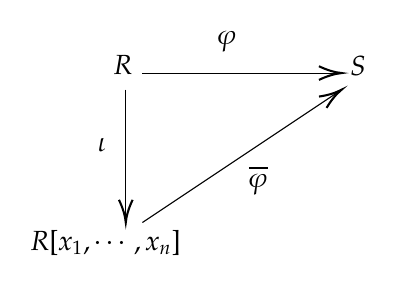
\begin{tikzpicture}[x=0.75pt,y=0.75pt,yscale=-1,xscale=1]
%uncomment if require: \path (0,476); %set diagram left start at 0, and has height of 476

%Straight Lines [id:da3152671411941921] 
\draw    (240,128) -- (334,128) ;
\draw [shift={(336,128)}, rotate = 180] [color={rgb, 255:red, 0; green, 0; blue, 0 }  ][line width=0.75]    (10.93,-3.29) .. controls (6.95,-1.4) and (3.31,-0.3) .. (0,0) .. controls (3.31,0.3) and (6.95,1.4) .. (10.93,3.29)   ;
%Straight Lines [id:da5751301154780408] 
\draw    (232,136) -- (232,198) ;
\draw [shift={(232,200)}, rotate = 270] [color={rgb, 255:red, 0; green, 0; blue, 0 }  ][line width=0.75]    (10.93,-3.29) .. controls (6.95,-1.4) and (3.31,-0.3) .. (0,0) .. controls (3.31,0.3) and (6.95,1.4) .. (10.93,3.29)   ;
%Straight Lines [id:da5543492055231241] 
\draw    (240,200) -- (334.34,137.11) ;
\draw [shift={(336,136)}, rotate = 146.31] [color={rgb, 255:red, 0; green, 0; blue, 0 }  ][line width=0.75]    (10.93,-3.29) .. controls (6.95,-1.4) and (3.31,-0.3) .. (0,0) .. controls (3.31,0.3) and (6.95,1.4) .. (10.93,3.29)   ;

% Text Node
\draw (225,118.4) node [anchor=north west][inner sep=0.75pt]    {$R$};
% Text Node
\draw (339,118.4) node [anchor=north west][inner sep=0.75pt]    {$S$};
% Text Node
\draw (217,158.4) node [anchor=north west][inner sep=0.75pt]    {$\iota $};
% Text Node
\draw (185,202.4) node [anchor=north west][inner sep=0.75pt]    {$R[ x_{1} ,\cdots ,x_{n}]$};
% Text Node
\draw (290,171.4) node [anchor=north west][inner sep=0.75pt]    {$\overline{\varphi }$};
% Text Node
\draw (275,106.4) node [anchor=north west][inner sep=0.75pt]    {$\varphi $};


\end{tikzpicture}
\end{center}
\begin{note}\em
Note that the map $R[x_1,\cdots,x_n]\to S$ given by $f\mapsto\varphi f(s_1,\cdots,s_n)$ is a homomorphism of rings even when $R$ and $S$ do not have identities.
\end{note}
A consequence of Theorem 4.64 may be illustrated by the following example. 
Let $R$ be a commutative ring and consider 
$$
f=x^2y+x^3y+x^4+xy+y^3+r\in R\left[ x,y \right] .
$$
Observe that 
$$
f=y^2+\left( x^3+x^2+x \right) y+\left( x^4+r \right) \in R\left[ x \right] \left[ y \right] ,f=x^4+yx^3+yx^2+yx+\left( y^2+r \right) \in R\left[ y,x \right] ,
$$
this suggests $R[x][y]\cong R[y][x]$. More generally, we have the following theorem: 
\begin{theorem}
Let $R$ be a commutative ring with identity and $n$ a positive integer. For each $1\le k<n$ there are isomorphisms of rings: 
$$
R\left[ x_1,\cdots ,x_k \right] \left[ x_{k+1},\cdots ,x_n \right] \cong R\left[ x_1,\cdots ,x_n \right] \cong R\left[ x_{k+1},\cdots x_n \right] \left[ x_1,\cdots ,x_k \right] .
$$
\end{theorem}
\begin{proof}
We use the universal properties to prove this statement. Let $\varphi:R\to S$ be an homomorphism of commutative rings with identity, then by Theorem 4.64 there exists $\overline{\varphi}:R[x_1,\cdots,x_n]\to S$ such that $\overline{\varphi}\mid_R=\varphi$ and $\overline{\varphi}(x_i)=s_i$ for all $1\le i\le n$. Now substitute $R$ with $R[x_1,\cdots,x_k]$ in $\varphi$ and obtain $\overline{\overline{\varphi}}:R[x_1,\cdots,x_k][x_{k+1},\cdots,x_n]\to S$ such that $\overline{\overline{\varphi}}\mid_R=\varphi$ and $\overline{\overline{\varphi}}(x_i)=s_i$ for $k+1\le i\le n$. Since $R[x_1,\cdots,x_n]$ is determined up to isomorphism by the universal property, we have $R\left[ x_1,\cdots ,x_k \right] \left[ x_{k+1},\cdots ,x_n \right] \cong R\left[ x_1,\cdots ,x_n \right] $. Similarly we may prove that $R\left[ x_{k+1},\cdots x_n \right] \left[ x_1,\cdots ,x_k \right] \cong R\left[ x_1,\cdots ,x_n \right] $.
\end{proof}
Since $R[x_1,\cdots,x_k]$ is considered as a subring of $R[x_1,\cdots,x_n]$, it is customary to identify the various polynomial rings under the isomorphisms stated in Theorem 4.65 and write $R[x_1,\cdots,x_k][x_{k+1},\cdots,x_n]=R[x_1,\cdots,x_n]$.\par
We now discuss the rings of formal power series.
\begin{theorem}
Let $R$ be a ring and denote by $R[[x]]$ the set of all sequences of elements of $R(a_0,a_1,\cdots)$.\par
(i) $R[[x]]$ is a ring with addition and multiplication defined by 
$$
\left( a_0,a_1,\cdots \right) +\left( b_0,b_1,\cdots \right) =\left( a_0+b_0,a_1+b_1,\cdots \right) 
$$
and 
$$
\left( a_0,a_1,\cdots \right) \left( b_0,b_1,\cdots \right) =\left( c_0,c_1,\cdots \right) ,c_n=\sum_{i+j=n}{a_ib_j},n=0,1,\cdots .
$$\par
(ii) The polynomial ring $R[x]$ is a subring of $R[[x]]$.\par
(iii) If $R$ is a commutative [resp. a ring with identity or a ring with no zero divisors or an integral domain], then so is $R[[x]]$.
\end{theorem}
\begin{proof}
(i) and (iii) are similar to the proof of Theorem 4.60. For (ii), consider the monomorphism $(a_0,a_1,\cdots,a_n)\mapsto(a_0,\cdots,a_n,0,\cdots)$.
\end{proof}
The ring $R[[x]]$ of Theorem 4.66 is called the \textbf{ring of formal power series} over the ring $R$. Its elements are called power series. If $R$ has an identity then the polynomial $x=(0,1_R,0,\cdots)\in R[[x]]$ is called an indeterminate. We shall also denote $(a_0,a_1,\cdots)\in R[[x]]$ as $\sum_{i=0}^\infty a_ix^i$, where $a_i$ are called \textbf{coefficients} and $a_0$ is called the constant term. This notation is also used when $R$ has no identity, with same reason to that of polynomials.
\begin{proposition}
Let $R$ be a ring with identity and $f=\sum_{i=0}^\infty a_ix^i\in R[[x]]$.\par
(i) $f$ is a unit in $R[[x]]$ if and only if its constant term $a_0$ is a unit in $R$.\par
(ii) If $a_0$ is irreducible in $R$, then $f$ is irreducible in $R[[x]]$.
\end{proposition}
\begin{proof}
(i) Suppose $f\in R[[x]]$ is a unit, then there exists some $g=\sum b_nx^n$ such that $fg=gf=1_R$. It follows immediately that $a_0b_0=b_0a_0=1_R$, whence $a_0$ is a unit in $R$. Conversely, it suffices to solve the equation below: 
$$
\begin{cases}
	a_0b_0=1_R,\\
	a_0b_1+a_1b_0=0,\\
	\vdots\\
	a_0b_n+a_1b_{n-1}+\cdots +a_nb_0=0,\\
	\vdots\\
\end{cases}
$$
Since $a_0$ is a unit, we have $b_0=a_0^{-1}$. Proceed inductively, we have $$b_n=a_{0}^{-1}\left( -a_1b_{n-1}-\cdots -a_nb_0 \right) ,$$
whence $g=\sum b_nx^n\in R[[x]]$ satisfies $fg=1_R$. Similarly we may find $h\in R[[x]]$ such that $hf=1_R$. However $h=h1_R=h(fg)=(hf)g=g$, therefore $fg=gf=1_R$ and the proof is finished.\par
(ii) follows directly from (i).
\end{proof}
\begin{corollary}
If $R$ is a division ring, then the units in $R[[x]]$ are precisely those power series with nonzero constant term. The principal ideal $(x)$ consists precisely of the nonunits in $R[[x]]$ and is the unique maximal ideal of $R[[x]]$. Thus if $R$ is a field, $R[[x]]$ is a local ring.
\end{corollary}
\begin{proof}
The first statement follows since $R$ is a division ring and Proposition 4.67 (i), since every nonzero element in a division ring is a unit. Since $x$ is in the center of $R[[x]]$, by Theorem 4.15 we have $(x)=\{xf:f\in R[[x]]\}$. Consequently, every element $xf$ of $(x)$ has zero constant term, whence $xf$ is a nonunit. Conversely every nonunit $f\in R[[x]]$ is necessarily of the form $f=\sum a_ix^i$ with $a_0=0$. Let $g=\sum b_ix^i$ where $b_i=a_{i+1}$ for all $i$. Then $xg=f$, whence $f\in (x)$. Therefore $(x)$ is the set of nonunits. Finally, since $1_R\notin(x)$, $(x)\ne R[[x]]$. Furthermore, every ideal $I$ of $R[[x]]$ with $I\ne R[[x]]$ necessarily consists of nonunits. Thus every ideal of $R[[x]]$ except $R[[x]]$ is contained in $(x)$. Therefore $R[[x]]$ is local.
\end{proof}
Some basic concepts, such as the degree of a polynomial, or the division algorithm has been introduced in the course of Linear Algebra, for which a reader may refer to any textbook of Advanced algebra, or Linear algebra. We mention an important result here: 
\begin{theorem}
If $D$ is a unique factorization domain, then so is the polynomial ring $D[x_1,\cdots,x_n]$.
\end{theorem}
We skip the proof of this result. A reader who wishes to scan the proof of this theorem may refer to GTM73 page 164. Note that a field $F$ is trivially a UFD, therefore if $F$ is a field, then the polynomial ring $F[x_1,\cdots,x_n]$ is a UFD.
\begin{center}
\begin{large}
    \textbf{Exercises for 4.5}
\end{large}
\end{center}
\begin{problem}\em
(a) If $\varphi:R\to S$ is a homomorphism of rings, then the map $\overline{\varphi}:R[[x]]\to S[[x]]$ given by $\overline{\varphi}\left(\sum a_ix^i\right)=\sum\varphi(a_i)x^i$ is a homomorphism of rings such that $\overline{\varphi}(R[x])\subset S[x]$.\par
(b) $\overline{\varphi}$ is a monomorphism [resp. epimorphism] if and only if $\varphi$ is. In this case $\varphi:R[x]\to S[x]$ is also a monomorphism [resp. epimorphism].\par
(c) Extend the results of (a) and (b) to polynomial rings $R[x_1,\cdots,x_n]$, $S[x_1,\cdots,x_n]$.
\end{problem}
\begin{proof}
(a) We only show that $\overline{\varphi}(fg)=\overline{\varphi}(f)\overline{\varphi}(g)$, where $f=\sum a_ix^i$ and $g=\sum b_ix^i$. It suffices to observe that 
$$
\begin{aligned}
\overline{\varphi }\left( fg \right) &=\overline{\varphi }\left( \sum{a_ix^i}\cdot \sum{b_ix^i} \right) =\overline{\varphi }\left( \sum{\sum_{i+j=n}{a_ib_j}x^n} \right) =\sum{\varphi \left( \sum_{i+j=n}{a_ib_j} \right) x^n}
\\
&=\sum{\sum_{i+j=n}{\varphi \left( a_ib_j \right) x^n}}=\sum{\sum_{i+j=n}{\varphi \left( a_i \right) \varphi \left( b_j \right) x^n}}=\overline{\varphi }\left( f \right) \overline{\varphi }\left( g \right) .
\end{aligned}
$$\par
(b) We only show the case that $\varphi$ is a monomorphism. First observe that 
$$
\overline{\varphi}\left( f \right) =\overline{\varphi }\left( g \right) \Leftrightarrow \sum{\varphi \left( a_i \right) x^i}=\sum{\varphi \left( b_i \right) x^i}\Leftrightarrow \varphi \left( a_i \right) =\varphi\left( b_i \right) .
$$
Therefore by the fact that $\varphi$ is monomorphism, we conclude that $\overline{\varphi}$ is a monomorphism.\par
(c) Let $f\in R[x_1,\cdots,x_n]$, with coefficients $a_i$. Then the map $\overline{\varphi}$ defined to map the coefficients $a_i$ into $\varphi(a_i)$ is a homomorphism of rings. An analogous statement may be made similar to (b).
\end{proof}
\begin{problem}\em
Let $\mathrm{Mat}_nR$ be the ring of $n\times n$ matrices over a ring $R$. Then for each $n\ge 1$, show that $(\mathrm{Mat}_nR)[x]\cong\mathrm{Mat}_nR[x]$ and $(\mathrm{Mat}_nR)[[x]]\cong\mathrm{Mat}_nR[[x]]$.
\end{problem}
\begin{proof}
We only prove that $(\mathrm{Mat}_nR)[x]\cong\mathrm{Mat}_nR[x]$, and the second statement may be prove analogously. Let $\sum A_ix^i\in(\mathrm{Mat}_nR)[x]$, and $A$ with its $(i,j)$ element $\sum a_{ij}^{(i)}x^i$, where $a_{ij}^{(i)}$ denote the $(i,j)$ element of $A_i$. Then the map $\varphi:\sum A_ix^i\mapsto A$ is an isomorphism. Therefore $(\mathrm{Mat}_nR)[x]\cong\mathrm{Mat}_nR[x]$.
\end{proof}
\begin{problem}\em
Let $R$ and $S$ be rings with identity, $\varphi:R\to S$ a homomorphism of rings with $\varphi(1_R)=\varphi(1_S)$, and $s_1,\cdots,s_n\in S$ such that $s_is_j=s_js_i$ for all $i,j$ and $\varphi(r)s_i=s_i\varphi(r)$ for all $r\in R$ and all $i$. Show that the ring $R[x_1,\cdots,x_n]$ has the universal property ans is uniquely determined by this property.
\end{problem}
\begin{proof}
Check the proof of Theorem 4.64, where only the commutativity of $s_i$ and $\varphi(r)$ is used, which satisfy the condition given here.
\end{proof}
\begin{problem}\em
(a) If $R$ is a ring of all $2\times 2$ matrices over $\mathbb{Z}$, then for all $A\in R$, $(x+A)(x-A)-x^2-A^2\in R[x]$.\par
(b) There exists $C,A\in R$ such that $(C+A)(C-A)\ne C^2-A^2$.
\end{problem}
\begin{proof}
(a) By trivial computation we get 
$$
\left( x+A \right) \left( x-A \right) =x^2-Ax+Ax-A^2=x^2-A^2\in R\left[ x \right] .
$$\par
(b) Consider 
$$
A=\left( \begin{matrix}
	1&		1\\
	1&		0\\
\end{matrix} \right) ,C=\left( \begin{matrix}
	1&		0\\
	0&		0\\
\end{matrix} \right) .
$$
\end{proof}
\begin{note}\em
This exercise offered an counterexample of Remark 4.29 when the ring is not commutative. 
\end{note}
\begin{problem}\em
If $R$ is a commutative ring with identity and $f=a_nx^n+\cdots+a_0$ is a zero divisor in $R[x]$, then there exists a nonzero $b\in R$ such that $ba_n=ba_{n-1}=\cdots=ba_0=0$.
\end{problem}
\begin{proof}
Since $f$ is a zero divisor of $R[x]$, then there exists some $g=b_mx^m+\cdots+b_0$ such that $fg=0$. Therefore take $b_0=b$, we have $ba_n=ba_{n-1}=\cdots=ba_0=0$.
\end{proof}
\begin{problem}\em
(a) The polynomial $x+1$ is a unit in the power series ring $\mathbb{Z}[[x]]$, but is not a unit in $\mathbb{Z}[x]$.\par
(b) $x^2+3x+2$ is irreducible in $\mathbb{Z}[[x]]$, but not in $\mathbb{Z}[x]$.
\end{problem}
\begin{proof}
(a) Clearly $x+1$ is not a unit in $\mathbb{Z}[x]$. Now observe that $(1+x)=(1-x)(1+x+x^2+\cdots)$, we have $1+x\in\mathbb{Z}[[x]]$ is a unit.\par
(b) In $\mathbb{Z}[x]$ we have $x^2+3x+2=(x+1)(x+2)$. However in $\mathbb{Z}[[x]]$, observe that $2$ is not a unit in $\mathbb{Z}$, we conclude that $x^2+3x+2$ is not a unit in $\mathbb{Z}[[x]]$.
\end{proof}
\begin{problem}\em
If $F$ is a field, then $(x)$ is a maximal ideal in $F[x]$, but it is not the only maximal ideal.
\end{problem}
\begin{proof}
We show that $F[x]/(x)\cong F$, whence $F[x]/(x)$ is a field, and hence $(x)$ is a maximal ideal of $F[x]$. Indeed, we may define an homomorphism $f:F[x]\to F$ that maps $f=a_0+a_1x+\cdots+a_nx^n$ to $a_0$, then the kernel of $f$ is $(x)$ and hence by the first isomorphism theorem we have $F[x]/(x)\cong F$, which finished the proof. Observe that in $\mathbb{R}[x]$ $(x+1)$ is also a maximal ideal of $\mathbb{R}[x]$.
\end{proof}
\newpage
\section{Modules}
In this chapter we introduce the concept of modules. Modules over a ring are a generalization of abelian groups (which are modules over $\mathbb{Z}$), where another proof of the factorization of finitely generated abelian groups is developed. The concept of modules are basic in the further study of algebra.
\subsection{Modules, Homomorphisms and Exact Sequences}
We first give the definition of a module.
\begin{definition}
Let $R$ be a ring, a (left) \textbf{$R$-module} is an additive abelian group $A$ together with a function $f:R\times A\to A$ (the image of $(r,a)$ is denoted as $ra$) such that for all $r,s\in R$ and $a,b\in A$ \par
(i) $r(a+b)=ra+rb$;\par
(ii) $(r+s)a=ra+sa$;\par
(iii) $r(sa)=(rs)a$.\par
If $R$ has an identity element $1_R$ and \par
(iv) $1_Ra=a$ for all $a\in A$,\par
then $A$ is said to be a \textbf{unitary $R$-module}. If $R$ is a division ring, then a unitary $R$-module is called a (left) vector space.
\end{definition}
A unitary right $R$-module is defined similarly via a function $A\times R\to A$ denoted $(a,r)\mapsto ar$ and satisfying the obvious analogous (i) to (iv). From now on, unless specified otherwise, $R$-module means left $R$-module and it is understood that all theorems about left $R$-modules also hold, \textit{mutatis mutandis}, for right $R$-modules.\par
A given group $A$ may have many different $R$-module structures. If $R$ is commutative, it is easy to verify that every left $R$-module $A$ can be given on the structure of a right $R$-module by defining $ar=ra$ for all $r\in R,a\in A$, where commutativity is needed in (iii). Now every module $A$ over a commutative ring $R$ is considered to be both left and right with $ar=ra$ for all $a\in A$ and $r\in R$.\par
\begin{example}\em
Every additive abelian group $G$ is a unitary $\mathbb{Z}$-module, with $na$ ($n\in\mathbb{Z}$ and $a\in G$) given by the usual definition for groups.
\end{example}
\begin{example}\em
If $S$ is a ring and $R$ is a subring of $S$, then $S$ is an $R$-module (but not vice versa) with $ra$ being multiplication on $S$. In particular, the polynomial ring $R[x_1,\cdots,x_n]$ and the formal power series ring $R[[x]]$ are $R$-modules.
\end{example}
\begin{example}\em
Let $R$ be a ring and $I$ be a left ideal of $R$. Then $I$ is an $R$-module with $ra\in I$ for all $r\in R$ and $a\in I$ under multiplication of $R$. In particular, $0$ and $R$ are trivial $R$-modules. Furthermore, since $I$ is an additive group, we have $R/I$ be an (abelian) group and an $R$-module with $r(r_1+I)=rr_1+I$. Note that $R/I$ need not to be a ring, unless $I$ is a two-sided ideal.
\end{example}
\begin{example}\em
Let $\varphi:R\to S$ be a ring homomorphism and let $A$ be an $S$-module. Then $A$ can be made into an $R$-module by defining $rx$ to be $\varphi(r)x$, where $r\in R$ and $x\in A$. One says that the $R$-module structure of $A$ is given by \textbf{pullback along $\varphi$}.
\end{example}
\begin{example}\em
Let $A$ be an abelian group and $\mathrm{End}A$ be its endomorphism ring. Then $A$ is a unitary $\mathrm{End}A$-module with $fa$ defined to be $f(a)$, where $a\in A$ and $f\in\mathrm{End}A$.
\end{example}
\begin{example}\em
If $R$ is a ring, every abelian group can be made into an $R$-module with trivial structure with $ra=0$ for all $r\in R$ and $a\in A$.
\end{example}
\begin{definition}
Let $A$ and $B$ be modules over a ring $R$. A function $f:A\to B$ is an \textbf{$R$-module homomorphism} provided that for all $a,c\in A$ and $r\in R$ we have $f(a+c)=f(a)+f(c)$ and $f(ra)=rf(a)$. If $R$ is a division ring, then an $R$-module homomorphism is called a \textbf{linear transformation}.
\end{definition}
When the context is clear we call an $R$-module homomorphism simply a homomorphism. By definition every $R$-module homomorphism is a homomorphism of abelian groups $A\to B$. Therefore the terminologies are used: an $R$-module homomorphism $f$ is an epimorphism [resp. monomorphism, isomorphism] if and only if $f$ is surjective [resp. injective, bijective] as a map of sets. The \textbf{kernel} of $f$ is its kernel as abelian groups, i.e. $\mathrm{Ker}f=\{a\in A:f(a)=0\}$. The \textbf{image} of $f$ is the set $\mathrm{Im}f=\{b\in B:b=f(a)\ \text{for some}\ a\in A\}$. We have the following propositions:
\begin{proposition}
$f$ is an $R$-module monomorphism [resp. isomorphism] if and only if $\mathrm{Ker}f=0$ [resp. there exists some $g:B\to A$ such that $fg=1_B$ and $gf=1_A$].
\end{proposition}
For a proof of this proposition, see Theorem 2.9. We now give some examples of homomorphisms of modules.
\begin{example}\em
For any modules the zero map $0:A\to B$ given by $a\mapsto 0$ is a trivial homomorphism. Every homomorphism of abelian groups is a homomorphism of $\mathbb{Z}$-module. If $R$ is a ring, then the map $R[x]\to R[x]$ given by $f\mapsto xf$ is a $R$-module homomorphism. Note that $f\mapsto xf$ is not a ring homomorphism.
\end{example}
Note that for a given ring $R$ the class of all $R$-modules [resp. unitary $R$-modules] and $R$-module homomorphisms clearly forms a (concrete) category.
\begin{definition}
Let $R$ be a ring, $A$ am $R$-module and $B$ a nonempty subset of $A$. $B$ is a \textbf{submodule} of $A$ provided that $B$ is an additive subgroup of $A$ and $rb\in B$ for all $r\in R$ and $b\in B$. A submodule of a vector space over a division ring is called a \textbf{subspace}.
\end{definition}
Note that a submodule itself is a module. Also a submodule of a unitary module over a ring with identity is necessarily unitary.
\begin{example}\em
Let $R$ be a ring and $f:A\to B$ is an $R$-module homomorphism, then $\mathrm{Ker}f$ is a submodule of $A$ and $\mathrm{Im}f$ is a submodule of $B$. If $C$ is a submodule of $B$, then $f^{-1}(C)$ is a submodule of $A$.
\end{example}
\begin{example}\em
If $R$ is a ring and $I$ is a left ideal of $R$, $A$ an $R$-module and $S$ a nonempty subset of $A$, then $IS=\left\{\sum_{i=1}^nr_ia_i:r_i\in I,a_i\in S,n\in\mathbb{N}_+\right\}$ is a submodule of $A$. Similarly if $a\in A$, then $Ia=\{ra:r\in I\}$ is a submodule of $A$.
\end{example}
\begin{example}\em
If $\{B_i:i\in I\}$ is a family of submodules of a module $A$, then $\bigcap_{i\in I}B_i$ is also a submodule of $A$.
\end{example}
\begin{definition}
If $X$ is a subset of a module $A$ over a ring $R$, then the intersection of all submodules of $A$ containing $X$ is called the \textbf{submodule generated by $X$} (or \textbf{spanned by $X$}).
\end{definition}
If $X$ is finite, and $X$ generates the module $B$, then $B$ is said to be \textbf{finitely generated}. If $X=\emptyset$, then $X$ clearly generates the zero module. If $X$ consists of a single element, i.e. $X=\{a\}$, then the submodule generated by $X$ is called the \textbf{cyclic (sub)module} generated by $a$. Finally, if $\{B_i:i\in I\}$ is a family of submodules of $A$, then the submodule generated by $X=\bigcup_{i\in I}B_i$ is called the \textbf{sum} of modules $B_i$. If the index is finite, the sum of $B_1,\cdots,B_n$ is denoted $B_1+B_2+\cdots+B_n$.\par
The next theorem gives some basic properties of submodules.
\begin{theorem}
Let $R$ be a ring, $A$ an $R$-module, $X$ a subset of $A$, $\{B_i:i\in I\}$ a family of submodules of $A$ and $a\in A$. Let $Ra=\{ra:r\in R\}$.\par
(i) $Ra$ is a submodule of $A$ and the map $R\to Ra$ given by $r\mapsto ra$ is an $R$-module epimorphism.\par
(ii) The cyclic submodule $C$ generated by $a$ is $\{ra+na:r\in R,n\in\mathbb{Z}\}$. If $R$ has an identity and $C$ is unitary, then $C=Ra$.\par
(iii) The submodule $D$ generated by $X$ is 
$$
\left\{ \sum_{i=1}^s{r_ia_i}+\sum_{j=1}^t{n_jb_j}:s,t\in \mathbb{N} _+,a_j,b_j\in X,r_i\in R,n_j\in \mathbb{Z} \right\} .
$$
If $R$ has an identity and $A$ is unitary, then 
$$
D=RX=\left\{ \sum_{i=1}^s{r_ia_i}:s\in \mathbb{N} _+,a_i\in X,r_i\in R \right\} .
$$\par
(iv) The sum of the family $\{B_i:i\in I\}$ consists of all finite sums $b_{i1}+\cdots+b_{in}$ with $b_{ik}\in B_{ik}$.
\end{theorem}
\begin{proof}
(i) We first show that $Ra$ is a submodule. Clearly $Ra$ is an abelian group. Now suppose $r\in R$ and $r^\prime a\in Ra$, then $rr^\prime a\in Ra$, whence $Ra$ is an $R$-submodule of $A$. Define $f:R\to Ra$ given by $r\mapsto ra$, then for all $ra\in Ra$ we have $f(r)=ra$, whence $f$ is an epimorphism.\par
(ii) It is easy to verify that $\{ra+na\}$ is a module over $R$. Suppose $A$ is the module generated by $a$, then $ra\in A$, $na\in A$. Therefore $ra+na\in A$, hence $\{ra+na\}$ is the smallest module generated by $a$, therefore $C=\{ra+na\}$. If $R$ has an identity and $R$ is a unitary module, then $na=(n1_R)a\in Ra$.\par
(iii) An similar proof to (ii) may be made to conclude the assertion. We skip the proof.\par
(iv) Since the sum of $\{B_i:i\in I\}$ is generated by all elements of $B_i$, therefore $b_{i1}+\cdots+b_{in}$ is an element of the module generated by all $B_i$.
\end{proof}
\begin{theorem}
Let $B$ be a submodule of a module $A$ over a ring $R$. Then the quotient group $A/B$ is an $R$-module with the action of $R$ on $A/B$ given by 
$$
r\left( a+B \right) =ra+B,r\in R,a\in A.
$$
The map $\pi:A\to A/B$ given by $a\mapsto a+B$ is an $R$-module epimorphism with kernel $B$.
\end{theorem}
\begin{proof}
We first show that the definitions here are well-defined. First, since $B$ is a submodule of $A$, then $B$ is an abelian group and $rb\in B$ for all $r\in R$ and $b\in B$. Therefore $B\lhd A$ and hence $A/B$ is well-defined. Now suppose $a+B=a^\prime+B$, then $a-a^\prime\in B$. Since $B$ is a module, then $r(a-a^\prime)\in B$ for all $r\in R$, whence $ra+B=ra^\prime+B$ and the action is well-defined. By definition it is easy to verify that $A/B$ is an $R$-module and $\pi$ is an epimorphism with $\mathrm{Ker}\pi=B$.
\end{proof}
\begin{note}\em
The map $\pi:A\to A/B$ is called the \textbf{canonical epimorphism} (or \textbf{projection}).
\end{note}
In view of the preceding results, it is not surprising that the various isomorphism theorems for groups are valid, \textit{mutatis mutandis}, for modules. One need only check at each stage of the proof to see that every subgroup of homomorphism is in fact a submodule or module homomorphism. We omit the results here. See Theorem 2.35 to Corollary 2.39.\par
Next we show that product and coproducts always exist in the category of $R$-modules.
\begin{theorem}
Let $R$ be a ring and $\{A_i:i\in I\}$ a nonempty family of $R$-modules, $\prod_{i\in I}A_i$ the direct product of the abelian groups $A_i$, and $\bigoplus_{i\in I}A_i$ the direct sum of the abelian groups $A_i$.\par
(i) $\prod_{i\in I}A_i$ is an $R$-module with the action of $R$ given by $r\{a_i\}=\{ra_i\}$.\par
(ii) $\bigoplus_{i\in I}A_i$ is a submodule of $\prod_{i\in I}A_i$.\par
(iii) For each $k\in I$, the canonical projection $\pi_k:\prod A_i\to A_k$ is an $R$-module epimorphism.\par
(iv) For each $k\in I$, the canonical injection $\iota_k:A_k\to\bigoplus A_i$ is an $R$-module monomorphism.
\end{theorem}
\begin{proof}
(i) Trivially $\prod A_i$ is an abelian group. By definition we have $A_i$ is an $R$-module, and hence $ra_i\in A_i$ for all $i\in I$. Therefore $r\{a_i\}=\{ra_i\}\in\prod A_i$ and hence $\prod A_i$ is an $R$-module with the given action.\par
(ii) By definition $\bigoplus A_i$ is a subgroup of $\prod A_i$. Note that for all $r\in R$ and $\{a_i\}_{i\in I}\in\bigoplus A_i$ we have $r\{a_i\}=\{ra_i\}\in\bigoplus A_i$, therefore $\bigoplus A_i$ is a submodule of $\prod A_i$.\par
(iii) and (iv) See section 2.8.
\end{proof}
$\prod A_i$ is called the (external) \textbf{direct product} of the family of $R$-modules $\{A_i:i\in I\}$ and $\bigoplus A_i$ is its (external) \textbf{direct sum}. If the index is finite, say $I=\{1,2,\cdots,n\}$, then the direct product and the direct sum coincide and will be written $A_1\oplus A_2\oplus\cdots\oplus A_n$. The maps $\pi_k$ [resp. $\iota_k$] are called the \textbf{canonical projections} [resp. \textbf{injections}]. Clearly, $\prod A_i$ and $\bigoplus A_i$ has the universal properties and is determined uniquely by this property.\par
Finite direct sums occur so frequently that a further discussion of them will be useful. We first observe that if $f$ and $g$ are $R$-module homomorphisms from an $R$-module $A$ to another $R$-module $B$, then the map $f+g:A\to B$ given by $a+b\mapsto f(a)+f(b)$ is also an $R$-module homomorphism. It is easy to verify that the set $\mathrm{Hom}_R(A,B)$ of all homomorphisms of $A$ to $B$ is an abelian group under the addition. Furthermore addition of module homomorphisms is distributive with respect to composition of functions, i.e. $h(f+g)=hf+hg$ and $(f+g)k=fk+gk$, where $f,g:A\to B$ and $h:B\to C$, $k:D\to A$.
\begin{theorem}
Let $R$ be a ring and $A_1,\cdots,A_n$ be $R$-modules. Then $A\cong A_1\oplus\cdots\oplus A_n$ if and only if for each $i=1,2,\cdots,n$ there are $R$-module homomorphisms $\pi_i:A\to A_i$, $\iota_i:A_i\to A$ such that \par
(i) $\pi_i\iota_i=1_{A_{i}}$ for all $i=1,2,\cdots,n$;\par
(ii) $\pi_j\iota_i=0$ for $i\ne j$;\par
(iii) $\iota_1\pi_1+\cdots+\iota_n\pi_n=1_A$.
\end{theorem}
\begin{proof}
To show the existence of $\pi_i$ and $\iota_i$, consider the canonical injections and canonical projections. Conversely, if there exists $\pi_i$ and $\iota_i$ satisfies (i), (ii) and (iii), then consider canonical injections $\pi_i^\prime$ and canonical projections $\iota_i^\prime$. Let $\varphi:A_1\oplus A_2\oplus\cdots\oplus A_n$ and $\psi:A\to A_1\oplus A_2\oplus\cdots\oplus A_n$ by $\iota_1^\prime\pi_1+\cdots+\iota_n^\prime\pi_n$, we have 
$$
\varphi \psi =\left( \sum_{i=1}^n{\iota _i\pi _{i}^{\prime}} \right) \left( \sum_{i=1}^n{\iota _{i}^{\prime}\pi _i} \right) =\sum_{i=1}^n{\sum_{j=1}^n{\iota _{i}^{\prime}\pi _i}\iota _j\pi _{j}^{\prime}}=\sum_{i=1}^n{\iota _i1_{A_i}\pi _i}=\sum_{i=1}^n{\iota _i\pi _i}=1_A,
$$
and similarly 
$$
\psi \varphi =\left( \sum_{i=1}^n{\iota _{i}^{\prime}\pi _i} \right) \left( \sum_{i=1}^n{\iota _i\pi _{i}^{\prime}} \right) =\sum_{i=1}^n{\sum_{i=1}^n{\iota _i\pi _{i}^{\prime}}\iota _{i}^{\prime}\pi _i}=1_{A_1\oplus A_2\oplus \cdots \oplus A_n}.
$$
Therefore $\varphi$ is an isomorphism and the proof is finished.
\end{proof}
\begin{theorem}
Let $R$ be a ring and $\{A_i:i\in I\}$ a family of submodules of an $R$-module $A$ such that $A$ is the sum of the family $\{A_i:i\in I\}$, and for each $k\in I$ we have $A_k\cap A_k^*=0$, where $A_k^*=\{A_i:i\ne k\}$, then there is an isomorphism $A\cong\bigoplus_{i\in I}A_i$.
\end{theorem}
The proof of this theorem may be referred to Theorem 2.68.\par
Note that there are also similar concepts of \textbf{internal direct product}, which is, indeed, isomorphic to the external direct product introduced before. However, note that the internal direct product of $\{A_i:i\in I\}$ does not actually contain $A_i$'s but only isomorphic pieces of it. The adjective internal and external are omitted when no confusion will be made in context.\par
We now introduce another important concept, which is very useful in homomorphic algebra: 
\begin{definition}
A pair of module homomorphisms, $A\overset{f}{\longrightarrow}B\overset{g}{\longrightarrow}C$, is said to be \textbf{exact} at $B$ provided $\mathrm{Im}f=\mathrm{Ker}g$. A finite sequence of module homomorphisms, $A_0\overset{f_1}{\longrightarrow}A_1\overset{f_2}{\longrightarrow}\cdots \overset{f_{n-1}}{\longrightarrow}A_{n-1}\overset{f_n}{\longrightarrow}A_n$, is \textbf{exact} provided $\mathrm{Im}f_i=\mathrm{Ker}f_{i+1}$ for $i=1,2,\cdots,n-1$. An infinite sequence of module homomorphisms, $\cdots \overset{f_{i-1}}{\longrightarrow}A_{i-1}\overset{f_i}{\longrightarrow}A_i\overset{f_{i+1}}{\longrightarrow}A_{i+1}\overset{f_{i+2}}{\longrightarrow}\cdots $ is \textbf{exact} provided $\mathrm{Im}f_i=\mathrm{Ker}f_{i+1}$ for all $i\in\mathbb{Z}$.
\end{definition}
When convenience we shall abuse the language slightly and refer to an exact sequence of modules rather than an exact sequence of module homomorphisms.
\begin{example}\em
Note first that for any module $A$, there are unique module homomorphisms $0\longrightarrow A$ and $A\longrightarrow 0$. If $A$ and $B$ are modules then the sequences $0\longrightarrow A\overset{\iota}{\longrightarrow}A\oplus B\overset{\pi}{\longrightarrow}B\longrightarrow 0$ and $0\longrightarrow B\overset{\iota}{\longrightarrow}A\oplus B\overset{\pi}{\longrightarrow}A\longrightarrow 0$ are exact, where the $\iota$'s and $\pi$'s are the canonical injections and projections respectively. Similarly, if $C$ is a submodule of $D$, then the sequence $0\longrightarrow C\overset{i}{\longrightarrow}D\overset{p}{\longrightarrow}D/C\longrightarrow 0$ is exact, there $i$ and $p$ are trivial injection and projection. If $f:A\to B$ is a module homomorphism, then $A/\mathrm{Ker}f$ [resp. $B/\mathrm{Im}f$] is called the \textbf{coimage} of $f$ [resp. \textbf{cokernel} of $f$] and denote as $\mathrm{CoIm}f$ [resp. $\mathrm{CoKer}f$]. Each of the following sequences is exact: $0\longrightarrow \mathrm{Ker}f\longrightarrow A\longrightarrow \mathrm{CoIm}f\longrightarrow 0$, $0\longrightarrow \mathrm{Im}f\longrightarrow B\longrightarrow \mathrm{CoKer}f\longrightarrow 0$ and $0\longrightarrow \mathrm{Ker}f\longrightarrow A\longrightarrow B\longrightarrow \mathrm{CoKer}f\longrightarrow 0$.
\end{example}
\begin{note}\em
$0\longrightarrow A\overset{f}{\longrightarrow}B$ is an exact sequence of module homomorphism if and only if $f$ is a module monomorphism. Similarly, $B\overset{g}{\longrightarrow}C\longrightarrow 0$ is exact if and only if $g$ is a module epimorphism. If $A\overset{f}{\longrightarrow}B\overset{g}{\longrightarrow}C$ is exact, then $gf=0$. Finally if $A\overset{f}{\longrightarrow}B\overset{g}{\longrightarrow}C\longrightarrow 0$ is exact, then 
$$
\mathrm{CoKer}f=B/\mathrm{Im}f=B/\mathrm{Ker}g=\mathrm{CoIm}g\cong C.
$$
An exact sequence of the form $0\longrightarrow A\overset{f}{\longrightarrow}B\overset{g}{\longrightarrow}C\longrightarrow 0$ is called a \textbf{short exact sequence}. Note that $f$ is a monomorphism and $g$ an epimorphism. The preceding remarks show that a short exact sequence is just another way of presenting a submodule ($A\cong\mathrm{Im}f$) and its quotient module ($B/\mathrm{Im}f=B/\mathrm{Ker}g\cong C$).
\end{note}
\begin{lemma}\em(The Short Five Lemma)
Let $R$ be a ring and 
\begin{center}


\tikzset{every picture/.style={line width=0.75pt}} %set default line width to 0.75pt        

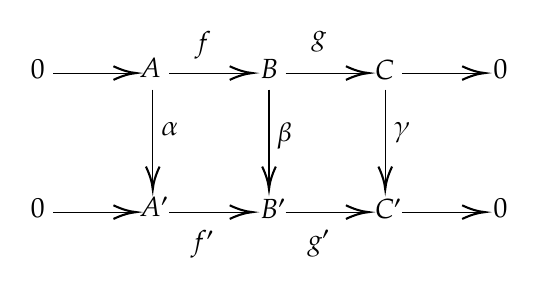
\begin{tikzpicture}[x=0.75pt,y=0.75pt,yscale=-1,xscale=1]
%uncomment if require: \path (0,476); %set diagram left start at 0, and has height of 476

%Straight Lines [id:da22573280049285005] 
\draw    (160,224) -- (198,224) ;
\draw [shift={(200,224)}, rotate = 180] [color={rgb, 255:red, 0; green, 0; blue, 0 }  ][line width=0.75]    (10.93,-3.29) .. controls (6.95,-1.4) and (3.31,-0.3) .. (0,0) .. controls (3.31,0.3) and (6.95,1.4) .. (10.93,3.29)   ;
%Straight Lines [id:da5007083409135236] 
\draw    (216,224) -- (254,224) ;
\draw [shift={(256,224)}, rotate = 180] [color={rgb, 255:red, 0; green, 0; blue, 0 }  ][line width=0.75]    (10.93,-3.29) .. controls (6.95,-1.4) and (3.31,-0.3) .. (0,0) .. controls (3.31,0.3) and (6.95,1.4) .. (10.93,3.29)   ;
%Straight Lines [id:da49627755138453633] 
\draw    (272,224) -- (310,224) ;
\draw [shift={(312,224)}, rotate = 180] [color={rgb, 255:red, 0; green, 0; blue, 0 }  ][line width=0.75]    (10.93,-3.29) .. controls (6.95,-1.4) and (3.31,-0.3) .. (0,0) .. controls (3.31,0.3) and (6.95,1.4) .. (10.93,3.29)   ;
%Straight Lines [id:da7229825431747845] 
\draw    (328,224) -- (366,224) ;
\draw [shift={(368,224)}, rotate = 180] [color={rgb, 255:red, 0; green, 0; blue, 0 }  ][line width=0.75]    (10.93,-3.29) .. controls (6.95,-1.4) and (3.31,-0.3) .. (0,0) .. controls (3.31,0.3) and (6.95,1.4) .. (10.93,3.29)   ;
%Straight Lines [id:da42771610429371165] 
\draw    (160,291) -- (198,291) ;
\draw [shift={(200,291)}, rotate = 180] [color={rgb, 255:red, 0; green, 0; blue, 0 }  ][line width=0.75]    (10.93,-3.29) .. controls (6.95,-1.4) and (3.31,-0.3) .. (0,0) .. controls (3.31,0.3) and (6.95,1.4) .. (10.93,3.29)   ;
%Straight Lines [id:da12408345309174651] 
\draw    (216,291) -- (254,291) ;
\draw [shift={(256,291)}, rotate = 180] [color={rgb, 255:red, 0; green, 0; blue, 0 }  ][line width=0.75]    (10.93,-3.29) .. controls (6.95,-1.4) and (3.31,-0.3) .. (0,0) .. controls (3.31,0.3) and (6.95,1.4) .. (10.93,3.29)   ;
%Straight Lines [id:da5038313801743268] 
\draw    (272,291) -- (310,291) ;
\draw [shift={(312,291)}, rotate = 180] [color={rgb, 255:red, 0; green, 0; blue, 0 }  ][line width=0.75]    (10.93,-3.29) .. controls (6.95,-1.4) and (3.31,-0.3) .. (0,0) .. controls (3.31,0.3) and (6.95,1.4) .. (10.93,3.29)   ;
%Straight Lines [id:da8627554494400742] 
\draw    (328,291) -- (366,291) ;
\draw [shift={(368,291)}, rotate = 180] [color={rgb, 255:red, 0; green, 0; blue, 0 }  ][line width=0.75]    (10.93,-3.29) .. controls (6.95,-1.4) and (3.31,-0.3) .. (0,0) .. controls (3.31,0.3) and (6.95,1.4) .. (10.93,3.29)   ;
%Straight Lines [id:da9219190287457819] 
\draw    (208,232) -- (208,278) ;
\draw [shift={(208,280)}, rotate = 270] [color={rgb, 255:red, 0; green, 0; blue, 0 }  ][line width=0.75]    (10.93,-3.29) .. controls (6.95,-1.4) and (3.31,-0.3) .. (0,0) .. controls (3.31,0.3) and (6.95,1.4) .. (10.93,3.29)   ;
%Straight Lines [id:da4241610695219813] 
\draw    (264,232) -- (264,278) ;
\draw [shift={(264,280)}, rotate = 270] [color={rgb, 255:red, 0; green, 0; blue, 0 }  ][line width=0.75]    (10.93,-3.29) .. controls (6.95,-1.4) and (3.31,-0.3) .. (0,0) .. controls (3.31,0.3) and (6.95,1.4) .. (10.93,3.29)   ;
%Straight Lines [id:da5742073517286415] 
\draw    (320,232) -- (320,278) ;
\draw [shift={(320,280)}, rotate = 270] [color={rgb, 255:red, 0; green, 0; blue, 0 }  ][line width=0.75]    (10.93,-3.29) .. controls (6.95,-1.4) and (3.31,-0.3) .. (0,0) .. controls (3.31,0.3) and (6.95,1.4) .. (10.93,3.29)   ;

% Text Node
\draw (148,216.4) node [anchor=north west][inner sep=0.75pt]    {$0$};
% Text Node
\draw (201,215.4) node [anchor=north west][inner sep=0.75pt]    {$A$};
% Text Node
\draw (259,216.4) node [anchor=north west][inner sep=0.75pt]    {$B$};
% Text Node
\draw (314,216.4) node [anchor=north west][inner sep=0.75pt]    {$C$};
% Text Node
\draw (371,216.4) node [anchor=north west][inner sep=0.75pt]    {$0$};
% Text Node
\draw (148,283.4) node [anchor=north west][inner sep=0.75pt]    {$0$};
% Text Node
\draw (201,282.4) node [anchor=north west][inner sep=0.75pt]    {$A^{\prime }$};
% Text Node
\draw (259,283.4) node [anchor=north west][inner sep=0.75pt]    {$B^{\prime }$};
% Text Node
\draw (314,283.4) node [anchor=north west][inner sep=0.75pt]    {$C^{\prime }$};
% Text Node
\draw (371,283.4) node [anchor=north west][inner sep=0.75pt]    {$0$};
% Text Node
\draw (227,202.4) node [anchor=north west][inner sep=0.75pt]    {$f$};
% Text Node
\draw (283,202.4) node [anchor=north west][inner sep=0.75pt]    {$g$};
% Text Node
\draw (225,298.4) node [anchor=north west][inner sep=0.75pt]    {$f^{\prime }$};
% Text Node
\draw (281,298.4) node [anchor=north west][inner sep=0.75pt]    {$g^{\prime }$};
% Text Node
\draw (211,246.4) node [anchor=north west][inner sep=0.75pt]    {$\alpha $};
% Text Node
\draw (267,246.4) node [anchor=north west][inner sep=0.75pt]    {$\beta $};
% Text Node
\draw (323,246.4) node [anchor=north west][inner sep=0.75pt]    {$\gamma $};


\end{tikzpicture}
\end{center}
a commutative diagram of $R$-modules and $R$-module homomorphisms such that each row is a short exact sequence. Then \par
(i) $\alpha,\gamma$ monomorphisms implies $\beta$ monomorphism;\par
(ii) $\alpha,\gamma$ epimorphisms implies $\beta$ epimorphism;\par
(iii) $\alpha,\gamma$ isomorphisms implies $\beta$ isomorphism.
\end{lemma}
\begin{proof}
(i) Suppose $\beta(b)=0$, we show that $b=0$. Observe that $g^{\prime}\circ \beta \left( b \right) =\gamma \circ g\left( b \right) =0$ we have $g(b)\in\mathrm{Ker}\gamma$. However $\gamma$ is a monomorphism and hence $\mathrm{Ker}\gamma=0$, therefore $g(b)=0$. Since the first row is exact we have $\mathrm{Ker}g=\mathrm{Im}f$, therefore there exists some $a\in A$ such that $f(a)=b$. Note that $\beta \circ f\left( a \right) =f^{\prime}\circ \alpha \left( a \right) =0$, we have $\alpha(a)\in\mathrm{Ker}f$. However $\mathrm{Ker}f=0$, we have $a=0$ and hence $b=f(a)=0$, therefore $\beta$ is a monomorphism.\par
(ii) Let $b^\prime\in B$, then $g^\prime(b)=c^\prime\in C^\prime$. Since $\gamma$ is an epimorphism, there exists some $c\in C$ such that $\gamma(c)=c^\prime$. Also suppose $g(b)=c$. Therefore $c^{\prime}=g^{\prime}\circ \beta \left( b \right) =\gamma \circ g\left( b \right) =\gamma \left( c \right) =g^{\prime}\left( b^{\prime} \right) $ and hence $g^\prime[\beta(b)-b^\prime]=0$ and $\beta(b)-b^\prime\in\mathrm{Ker}g^\prime$. Since the bottom row is exact we have $\mathrm{Ker}g^\prime=\mathrm{Im}f^\prime$ and hence there exists some $a^\prime\in A^\prime$ such that $f^\prime(a^\prime)=\beta(b)-b^\prime$. Since $\alpha$ is an epimorphism let $a^\prime=\alpha(a)$ for some $a\in A$. Consider $b-f(a)\in B$, we have 
$$
\beta \left[ b-f\left( a \right) \right] =\beta \left( b \right) -\beta \circ f\left( a \right) =\beta \left( b \right) -\beta \left( b \right) +b^{\prime}=b^{\prime},
$$
which finished the proof.\par
(iii) By (i) and (ii), the condition is trivial.
\end{proof}
Two short exact sequences are said to be \textbf{isomorphic} if there is a commutative diagram of module homomorphisms 
\begin{center}


\tikzset{every picture/.style={line width=0.75pt}} %set default line width to 0.75pt        

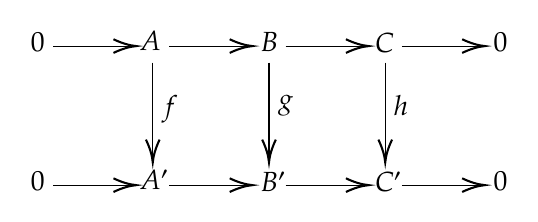
\begin{tikzpicture}[x=0.75pt,y=0.75pt,yscale=-1,xscale=1]
%uncomment if require: \path (0,476); %set diagram left start at 0, and has height of 476

%Straight Lines [id:da22573280049285005] 
\draw    (160,224) -- (198,224) ;
\draw [shift={(200,224)}, rotate = 180] [color={rgb, 255:red, 0; green, 0; blue, 0 }  ][line width=0.75]    (10.93,-3.29) .. controls (6.95,-1.4) and (3.31,-0.3) .. (0,0) .. controls (3.31,0.3) and (6.95,1.4) .. (10.93,3.29)   ;
%Straight Lines [id:da5007083409135236] 
\draw    (216,224) -- (254,224) ;
\draw [shift={(256,224)}, rotate = 180] [color={rgb, 255:red, 0; green, 0; blue, 0 }  ][line width=0.75]    (10.93,-3.29) .. controls (6.95,-1.4) and (3.31,-0.3) .. (0,0) .. controls (3.31,0.3) and (6.95,1.4) .. (10.93,3.29)   ;
%Straight Lines [id:da49627755138453633] 
\draw    (272,224) -- (310,224) ;
\draw [shift={(312,224)}, rotate = 180] [color={rgb, 255:red, 0; green, 0; blue, 0 }  ][line width=0.75]    (10.93,-3.29) .. controls (6.95,-1.4) and (3.31,-0.3) .. (0,0) .. controls (3.31,0.3) and (6.95,1.4) .. (10.93,3.29)   ;
%Straight Lines [id:da7229825431747845] 
\draw    (328,224) -- (366,224) ;
\draw [shift={(368,224)}, rotate = 180] [color={rgb, 255:red, 0; green, 0; blue, 0 }  ][line width=0.75]    (10.93,-3.29) .. controls (6.95,-1.4) and (3.31,-0.3) .. (0,0) .. controls (3.31,0.3) and (6.95,1.4) .. (10.93,3.29)   ;
%Straight Lines [id:da42771610429371165] 
\draw    (160,291) -- (198,291) ;
\draw [shift={(200,291)}, rotate = 180] [color={rgb, 255:red, 0; green, 0; blue, 0 }  ][line width=0.75]    (10.93,-3.29) .. controls (6.95,-1.4) and (3.31,-0.3) .. (0,0) .. controls (3.31,0.3) and (6.95,1.4) .. (10.93,3.29)   ;
%Straight Lines [id:da12408345309174651] 
\draw    (216,291) -- (254,291) ;
\draw [shift={(256,291)}, rotate = 180] [color={rgb, 255:red, 0; green, 0; blue, 0 }  ][line width=0.75]    (10.93,-3.29) .. controls (6.95,-1.4) and (3.31,-0.3) .. (0,0) .. controls (3.31,0.3) and (6.95,1.4) .. (10.93,3.29)   ;
%Straight Lines [id:da5038313801743268] 
\draw    (272,291) -- (310,291) ;
\draw [shift={(312,291)}, rotate = 180] [color={rgb, 255:red, 0; green, 0; blue, 0 }  ][line width=0.75]    (10.93,-3.29) .. controls (6.95,-1.4) and (3.31,-0.3) .. (0,0) .. controls (3.31,0.3) and (6.95,1.4) .. (10.93,3.29)   ;
%Straight Lines [id:da8627554494400742] 
\draw    (328,291) -- (366,291) ;
\draw [shift={(368,291)}, rotate = 180] [color={rgb, 255:red, 0; green, 0; blue, 0 }  ][line width=0.75]    (10.93,-3.29) .. controls (6.95,-1.4) and (3.31,-0.3) .. (0,0) .. controls (3.31,0.3) and (6.95,1.4) .. (10.93,3.29)   ;
%Straight Lines [id:da9219190287457819] 
\draw    (208,232) -- (208,278) ;
\draw [shift={(208,280)}, rotate = 270] [color={rgb, 255:red, 0; green, 0; blue, 0 }  ][line width=0.75]    (10.93,-3.29) .. controls (6.95,-1.4) and (3.31,-0.3) .. (0,0) .. controls (3.31,0.3) and (6.95,1.4) .. (10.93,3.29)   ;
%Straight Lines [id:da4241610695219813] 
\draw    (264,232) -- (264,278) ;
\draw [shift={(264,280)}, rotate = 270] [color={rgb, 255:red, 0; green, 0; blue, 0 }  ][line width=0.75]    (10.93,-3.29) .. controls (6.95,-1.4) and (3.31,-0.3) .. (0,0) .. controls (3.31,0.3) and (6.95,1.4) .. (10.93,3.29)   ;
%Straight Lines [id:da5742073517286415] 
\draw    (320,232) -- (320,278) ;
\draw [shift={(320,280)}, rotate = 270] [color={rgb, 255:red, 0; green, 0; blue, 0 }  ][line width=0.75]    (10.93,-3.29) .. controls (6.95,-1.4) and (3.31,-0.3) .. (0,0) .. controls (3.31,0.3) and (6.95,1.4) .. (10.93,3.29)   ;

% Text Node
\draw (148,216.4) node [anchor=north west][inner sep=0.75pt]    {$0$};
% Text Node
\draw (201,215.4) node [anchor=north west][inner sep=0.75pt]    {$A$};
% Text Node
\draw (259,216.4) node [anchor=north west][inner sep=0.75pt]    {$B$};
% Text Node
\draw (314,216.4) node [anchor=north west][inner sep=0.75pt]    {$C$};
% Text Node
\draw (371,216.4) node [anchor=north west][inner sep=0.75pt]    {$0$};
% Text Node
\draw (148,283.4) node [anchor=north west][inner sep=0.75pt]    {$0$};
% Text Node
\draw (201,282.4) node [anchor=north west][inner sep=0.75pt]    {$A^{\prime }$};
% Text Node
\draw (259,283.4) node [anchor=north west][inner sep=0.75pt]    {$B^{\prime }$};
% Text Node
\draw (314,283.4) node [anchor=north west][inner sep=0.75pt]    {$C^{\prime }$};
% Text Node
\draw (371,283.4) node [anchor=north west][inner sep=0.75pt]    {$0$};
% Text Node
\draw (211,246.4) node [anchor=north west][inner sep=0.75pt]    {$f$};
% Text Node
\draw (267,246.4) node [anchor=north west][inner sep=0.75pt]    {$g$};
% Text Node
\draw (323,246.4) node [anchor=north west][inner sep=0.75pt]    {$h$};


\end{tikzpicture}
\end{center}
such that $f,g$ and $h$ are isomorphisms. In this case, it is easy to verify that the diagram 
\begin{center}


\tikzset{every picture/.style={line width=0.75pt}} %set default line width to 0.75pt        

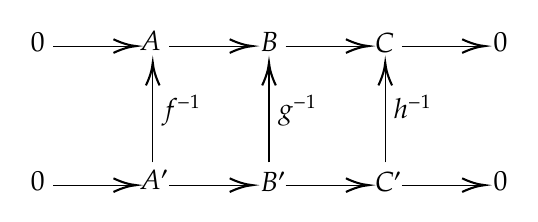
\begin{tikzpicture}[x=0.75pt,y=0.75pt,yscale=-1,xscale=1]
%uncomment if require: \path (0,476); %set diagram left start at 0, and has height of 476

%Straight Lines [id:da22573280049285005] 
\draw    (160,224) -- (198,224) ;
\draw [shift={(200,224)}, rotate = 180] [color={rgb, 255:red, 0; green, 0; blue, 0 }  ][line width=0.75]    (10.93,-3.29) .. controls (6.95,-1.4) and (3.31,-0.3) .. (0,0) .. controls (3.31,0.3) and (6.95,1.4) .. (10.93,3.29)   ;
%Straight Lines [id:da5007083409135236] 
\draw    (216,224) -- (254,224) ;
\draw [shift={(256,224)}, rotate = 180] [color={rgb, 255:red, 0; green, 0; blue, 0 }  ][line width=0.75]    (10.93,-3.29) .. controls (6.95,-1.4) and (3.31,-0.3) .. (0,0) .. controls (3.31,0.3) and (6.95,1.4) .. (10.93,3.29)   ;
%Straight Lines [id:da49627755138453633] 
\draw    (272,224) -- (310,224) ;
\draw [shift={(312,224)}, rotate = 180] [color={rgb, 255:red, 0; green, 0; blue, 0 }  ][line width=0.75]    (10.93,-3.29) .. controls (6.95,-1.4) and (3.31,-0.3) .. (0,0) .. controls (3.31,0.3) and (6.95,1.4) .. (10.93,3.29)   ;
%Straight Lines [id:da7229825431747845] 
\draw    (328,224) -- (366,224) ;
\draw [shift={(368,224)}, rotate = 180] [color={rgb, 255:red, 0; green, 0; blue, 0 }  ][line width=0.75]    (10.93,-3.29) .. controls (6.95,-1.4) and (3.31,-0.3) .. (0,0) .. controls (3.31,0.3) and (6.95,1.4) .. (10.93,3.29)   ;
%Straight Lines [id:da42771610429371165] 
\draw    (160,291) -- (198,291) ;
\draw [shift={(200,291)}, rotate = 180] [color={rgb, 255:red, 0; green, 0; blue, 0 }  ][line width=0.75]    (10.93,-3.29) .. controls (6.95,-1.4) and (3.31,-0.3) .. (0,0) .. controls (3.31,0.3) and (6.95,1.4) .. (10.93,3.29)   ;
%Straight Lines [id:da12408345309174651] 
\draw    (216,291) -- (254,291) ;
\draw [shift={(256,291)}, rotate = 180] [color={rgb, 255:red, 0; green, 0; blue, 0 }  ][line width=0.75]    (10.93,-3.29) .. controls (6.95,-1.4) and (3.31,-0.3) .. (0,0) .. controls (3.31,0.3) and (6.95,1.4) .. (10.93,3.29)   ;
%Straight Lines [id:da5038313801743268] 
\draw    (272,291) -- (310,291) ;
\draw [shift={(312,291)}, rotate = 180] [color={rgb, 255:red, 0; green, 0; blue, 0 }  ][line width=0.75]    (10.93,-3.29) .. controls (6.95,-1.4) and (3.31,-0.3) .. (0,0) .. controls (3.31,0.3) and (6.95,1.4) .. (10.93,3.29)   ;
%Straight Lines [id:da8627554494400742] 
\draw    (328,291) -- (366,291) ;
\draw [shift={(368,291)}, rotate = 180] [color={rgb, 255:red, 0; green, 0; blue, 0 }  ][line width=0.75]    (10.93,-3.29) .. controls (6.95,-1.4) and (3.31,-0.3) .. (0,0) .. controls (3.31,0.3) and (6.95,1.4) .. (10.93,3.29)   ;
%Straight Lines [id:da9219190287457819] 
\draw    (208,280) -- (208,234) ;
\draw [shift={(208,232)}, rotate = 90] [color={rgb, 255:red, 0; green, 0; blue, 0 }  ][line width=0.75]    (10.93,-3.29) .. controls (6.95,-1.4) and (3.31,-0.3) .. (0,0) .. controls (3.31,0.3) and (6.95,1.4) .. (10.93,3.29)   ;
%Straight Lines [id:da3968821204612032] 
\draw    (264,280) -- (264,234) ;
\draw [shift={(264,232)}, rotate = 90] [color={rgb, 255:red, 0; green, 0; blue, 0 }  ][line width=0.75]    (10.93,-3.29) .. controls (6.95,-1.4) and (3.31,-0.3) .. (0,0) .. controls (3.31,0.3) and (6.95,1.4) .. (10.93,3.29)   ;
%Straight Lines [id:da09148833810965606] 
\draw    (320,280) -- (320,234) ;
\draw [shift={(320,232)}, rotate = 90] [color={rgb, 255:red, 0; green, 0; blue, 0 }  ][line width=0.75]    (10.93,-3.29) .. controls (6.95,-1.4) and (3.31,-0.3) .. (0,0) .. controls (3.31,0.3) and (6.95,1.4) .. (10.93,3.29)   ;

% Text Node
\draw (148,216.4) node [anchor=north west][inner sep=0.75pt]    {$0$};
% Text Node
\draw (201,215.4) node [anchor=north west][inner sep=0.75pt]    {$A$};
% Text Node
\draw (259,216.4) node [anchor=north west][inner sep=0.75pt]    {$B$};
% Text Node
\draw (314,216.4) node [anchor=north west][inner sep=0.75pt]    {$C$};
% Text Node
\draw (371,216.4) node [anchor=north west][inner sep=0.75pt]    {$0$};
% Text Node
\draw (148,283.4) node [anchor=north west][inner sep=0.75pt]    {$0$};
% Text Node
\draw (201,282.4) node [anchor=north west][inner sep=0.75pt]    {$A^{\prime }$};
% Text Node
\draw (259,283.4) node [anchor=north west][inner sep=0.75pt]    {$B^{\prime }$};
% Text Node
\draw (314,283.4) node [anchor=north west][inner sep=0.75pt]    {$C^{\prime }$};
% Text Node
\draw (371,283.4) node [anchor=north west][inner sep=0.75pt]    {$0$};
% Text Node
\draw (211,246.4) node [anchor=north west][inner sep=0.75pt]    {$f^{-1}$};
% Text Node
\draw (267,246.4) node [anchor=north west][inner sep=0.75pt]    {$g^{-1}$};
% Text Node
\draw (323,246.4) node [anchor=north west][inner sep=0.75pt]    {$h^{-1}$};


\end{tikzpicture}
\end{center}
(with the same horizontal maps) is also commutative. In fact, isomorphism of short exact sequences is an equivalent relation.
\begin{theorem}
Let $R$ be a ring and $0\longrightarrow A_1\overset{f}{\longrightarrow}B\overset{g}{\longrightarrow}A_2\longrightarrow 0$ a short exact sequence of $R$-module homomorphisms. Then the following conditions are equivalent.\par
(i) There is an $R$-module homomorphism $h:A_2\to B$ with $gh=1_{A_2}$.\par
(ii) There is an $R$-module homomorphism $k:B\to A_1$ with $kf=1_{A_1}$.\par
(iii) The given sequence is isomorphic to the direct sum short exact sequence $0\longrightarrow A_1\overset{\iota _1}{\longrightarrow}A_1\oplus A_2\overset{\pi _2}{\longrightarrow}A_2\longrightarrow 0$. In particular $B\cong A_1\oplus A_2$.
\end{theorem}
\begin{proof}
(i)$\Rightarrow$(iii): Define the map $\varphi:A_1\oplus A_2\to B$ given by $(a_1,a_2)\mapsto f(a_1)+h(a_2)$. Therefore the diagram 
\begin{center}


\tikzset{every picture/.style={line width=0.75pt}} %set default line width to 0.75pt        

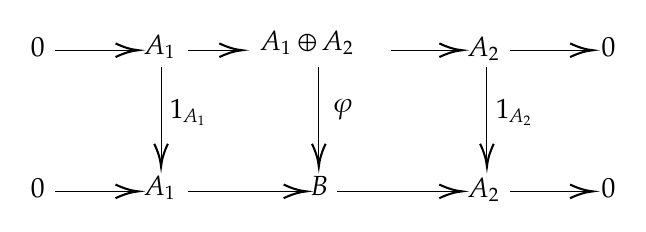
\begin{tikzpicture}[x=0.75pt,y=0.75pt,yscale=-1,xscale=1]
%uncomment if require: \path (0,476); %set diagram left start at 0, and has height of 476

%Straight Lines [id:da22573280049285005] 
\draw    (134,224) -- (172,224) ;
\draw [shift={(174,224)}, rotate = 180] [color={rgb, 255:red, 0; green, 0; blue, 0 }  ][line width=0.75]    (10.93,-3.29) .. controls (6.95,-1.4) and (3.31,-0.3) .. (0,0) .. controls (3.31,0.3) and (6.95,1.4) .. (10.93,3.29)   ;
%Straight Lines [id:da5007083409135236] 
\draw    (198,224) -- (222,224) ;
\draw [shift={(224,224)}, rotate = 180] [color={rgb, 255:red, 0; green, 0; blue, 0 }  ][line width=0.75]    (10.93,-3.29) .. controls (6.95,-1.4) and (3.31,-0.3) .. (0,0) .. controls (3.31,0.3) and (6.95,1.4) .. (10.93,3.29)   ;
%Straight Lines [id:da49627755138453633] 
\draw    (296,224) -- (328,224) ;
\draw [shift={(330,224)}, rotate = 180] [color={rgb, 255:red, 0; green, 0; blue, 0 }  ][line width=0.75]    (10.93,-3.29) .. controls (6.95,-1.4) and (3.31,-0.3) .. (0,0) .. controls (3.31,0.3) and (6.95,1.4) .. (10.93,3.29)   ;
%Straight Lines [id:da7229825431747845] 
\draw    (353,224) -- (391,224) ;
\draw [shift={(393,224)}, rotate = 180] [color={rgb, 255:red, 0; green, 0; blue, 0 }  ][line width=0.75]    (10.93,-3.29) .. controls (6.95,-1.4) and (3.31,-0.3) .. (0,0) .. controls (3.31,0.3) and (6.95,1.4) .. (10.93,3.29)   ;
%Straight Lines [id:da9219190287457819] 
\draw    (185,232) -- (185,278) ;
\draw [shift={(185,280)}, rotate = 270] [color={rgb, 255:red, 0; green, 0; blue, 0 }  ][line width=0.75]    (10.93,-3.29) .. controls (6.95,-1.4) and (3.31,-0.3) .. (0,0) .. controls (3.31,0.3) and (6.95,1.4) .. (10.93,3.29)   ;
%Straight Lines [id:da4241610695219813] 
\draw    (261,232) -- (261,278) ;
\draw [shift={(261,280)}, rotate = 270] [color={rgb, 255:red, 0; green, 0; blue, 0 }  ][line width=0.75]    (10.93,-3.29) .. controls (6.95,-1.4) and (3.31,-0.3) .. (0,0) .. controls (3.31,0.3) and (6.95,1.4) .. (10.93,3.29)   ;
%Straight Lines [id:da5742073517286415] 
\draw    (342,232) -- (342,278) ;
\draw [shift={(342,280)}, rotate = 270] [color={rgb, 255:red, 0; green, 0; blue, 0 }  ][line width=0.75]    (10.93,-3.29) .. controls (6.95,-1.4) and (3.31,-0.3) .. (0,0) .. controls (3.31,0.3) and (6.95,1.4) .. (10.93,3.29)   ;
%Straight Lines [id:da062379905314969175] 
\draw    (134,292) -- (172,292) ;
\draw [shift={(174,292)}, rotate = 180] [color={rgb, 255:red, 0; green, 0; blue, 0 }  ][line width=0.75]    (10.93,-3.29) .. controls (6.95,-1.4) and (3.31,-0.3) .. (0,0) .. controls (3.31,0.3) and (6.95,1.4) .. (10.93,3.29)   ;
%Straight Lines [id:da2958761370037739] 
\draw    (198,292) -- (253,292) ;
\draw [shift={(255,292)}, rotate = 180] [color={rgb, 255:red, 0; green, 0; blue, 0 }  ][line width=0.75]    (10.93,-3.29) .. controls (6.95,-1.4) and (3.31,-0.3) .. (0,0) .. controls (3.31,0.3) and (6.95,1.4) .. (10.93,3.29)   ;
%Straight Lines [id:da3240286217569581] 
\draw    (270,292) -- (328,292) ;
\draw [shift={(330,292)}, rotate = 180] [color={rgb, 255:red, 0; green, 0; blue, 0 }  ][line width=0.75]    (10.93,-3.29) .. controls (6.95,-1.4) and (3.31,-0.3) .. (0,0) .. controls (3.31,0.3) and (6.95,1.4) .. (10.93,3.29)   ;
%Straight Lines [id:da0337697350918047] 
\draw    (353,292) -- (391,292) ;
\draw [shift={(393,292)}, rotate = 180] [color={rgb, 255:red, 0; green, 0; blue, 0 }  ][line width=0.75]    (10.93,-3.29) .. controls (6.95,-1.4) and (3.31,-0.3) .. (0,0) .. controls (3.31,0.3) and (6.95,1.4) .. (10.93,3.29)   ;

% Text Node
\draw (121,216.4) node [anchor=north west][inner sep=0.75pt]    {$0$};
% Text Node
\draw (176,215.4) node [anchor=north west][inner sep=0.75pt]    {$A_{1}$};
% Text Node
\draw (232,213.4) node [anchor=north west][inner sep=0.75pt]    {$A_{1} \oplus A_{2}$};
% Text Node
\draw (332,216.4) node [anchor=north west][inner sep=0.75pt]    {$A_{2}$};
% Text Node
\draw (396,216.4) node [anchor=north west][inner sep=0.75pt]    {$0$};
% Text Node
\draw (188,246.4) node [anchor=north west][inner sep=0.75pt]    {$1_{A_{1}}$};
% Text Node
\draw (267,246.4) node [anchor=north west][inner sep=0.75pt]    {$\varphi $};
% Text Node
\draw (345,246.4) node [anchor=north west][inner sep=0.75pt]    {$1_{A_{2}}$};
% Text Node
\draw (121,284.4) node [anchor=north west][inner sep=0.75pt]    {$0$};
% Text Node
\draw (176,283.4) node [anchor=north west][inner sep=0.75pt]    {$A_{1}$};
% Text Node
\draw (256,283.4) node [anchor=north west][inner sep=0.75pt]    {$B$};
% Text Node
\draw (332,284.4) node [anchor=north west][inner sep=0.75pt]    {$A_{2}$};
% Text Node
\draw (396,284.4) node [anchor=north west][inner sep=0.75pt]    {$0$};


\end{tikzpicture}
\end{center}
is commutative, whence by the Short Five Lemma we have the two short exact sequence are isomorphic.\par
(ii)$\Rightarrow$(iii): Define $\psi:B\to A_1\oplus A_2$ by $b\mapsto(k(b),g(b))$. Observe that the diagram 
\begin{center}


\tikzset{every picture/.style={line width=0.75pt}} %set default line width to 0.75pt        

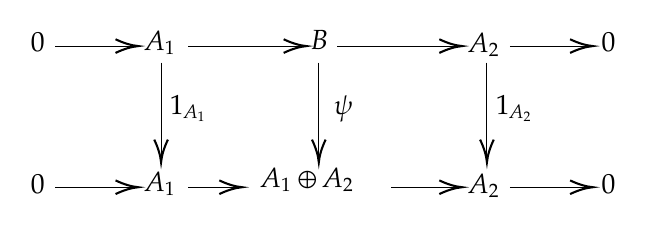
\begin{tikzpicture}[x=0.75pt,y=0.75pt,yscale=-1,xscale=1]
%uncomment if require: \path (0,476); %set diagram left start at 0, and has height of 476

%Straight Lines [id:da22573280049285005] 
\draw    (134,224) -- (172,224) ;
\draw [shift={(174,224)}, rotate = 180] [color={rgb, 255:red, 0; green, 0; blue, 0 }  ][line width=0.75]    (10.93,-3.29) .. controls (6.95,-1.4) and (3.31,-0.3) .. (0,0) .. controls (3.31,0.3) and (6.95,1.4) .. (10.93,3.29)   ;
%Straight Lines [id:da5007083409135236] 
\draw    (198,292) -- (222,292) ;
\draw [shift={(224,292)}, rotate = 180] [color={rgb, 255:red, 0; green, 0; blue, 0 }  ][line width=0.75]    (10.93,-3.29) .. controls (6.95,-1.4) and (3.31,-0.3) .. (0,0) .. controls (3.31,0.3) and (6.95,1.4) .. (10.93,3.29)   ;
%Straight Lines [id:da49627755138453633] 
\draw    (296,292) -- (328,292) ;
\draw [shift={(330,292)}, rotate = 180] [color={rgb, 255:red, 0; green, 0; blue, 0 }  ][line width=0.75]    (10.93,-3.29) .. controls (6.95,-1.4) and (3.31,-0.3) .. (0,0) .. controls (3.31,0.3) and (6.95,1.4) .. (10.93,3.29)   ;
%Straight Lines [id:da7229825431747845] 
\draw    (353,224) -- (391,224) ;
\draw [shift={(393,224)}, rotate = 180] [color={rgb, 255:red, 0; green, 0; blue, 0 }  ][line width=0.75]    (10.93,-3.29) .. controls (6.95,-1.4) and (3.31,-0.3) .. (0,0) .. controls (3.31,0.3) and (6.95,1.4) .. (10.93,3.29)   ;
%Straight Lines [id:da9219190287457819] 
\draw    (185,232) -- (185,278) ;
\draw [shift={(185,280)}, rotate = 270] [color={rgb, 255:red, 0; green, 0; blue, 0 }  ][line width=0.75]    (10.93,-3.29) .. controls (6.95,-1.4) and (3.31,-0.3) .. (0,0) .. controls (3.31,0.3) and (6.95,1.4) .. (10.93,3.29)   ;
%Straight Lines [id:da4241610695219813] 
\draw    (261,232) -- (261,278) ;
\draw [shift={(261,280)}, rotate = 270] [color={rgb, 255:red, 0; green, 0; blue, 0 }  ][line width=0.75]    (10.93,-3.29) .. controls (6.95,-1.4) and (3.31,-0.3) .. (0,0) .. controls (3.31,0.3) and (6.95,1.4) .. (10.93,3.29)   ;
%Straight Lines [id:da5742073517286415] 
\draw    (342,232) -- (342,278) ;
\draw [shift={(342,280)}, rotate = 270] [color={rgb, 255:red, 0; green, 0; blue, 0 }  ][line width=0.75]    (10.93,-3.29) .. controls (6.95,-1.4) and (3.31,-0.3) .. (0,0) .. controls (3.31,0.3) and (6.95,1.4) .. (10.93,3.29)   ;
%Straight Lines [id:da062379905314969175] 
\draw    (134,292) -- (172,292) ;
\draw [shift={(174,292)}, rotate = 180] [color={rgb, 255:red, 0; green, 0; blue, 0 }  ][line width=0.75]    (10.93,-3.29) .. controls (6.95,-1.4) and (3.31,-0.3) .. (0,0) .. controls (3.31,0.3) and (6.95,1.4) .. (10.93,3.29)   ;
%Straight Lines [id:da0337697350918047] 
\draw    (353,292) -- (391,292) ;
\draw [shift={(393,292)}, rotate = 180] [color={rgb, 255:red, 0; green, 0; blue, 0 }  ][line width=0.75]    (10.93,-3.29) .. controls (6.95,-1.4) and (3.31,-0.3) .. (0,0) .. controls (3.31,0.3) and (6.95,1.4) .. (10.93,3.29)   ;
%Straight Lines [id:da7190763458830736] 
\draw    (198,224) -- (253,224) ;
\draw [shift={(255,224)}, rotate = 180] [color={rgb, 255:red, 0; green, 0; blue, 0 }  ][line width=0.75]    (10.93,-3.29) .. controls (6.95,-1.4) and (3.31,-0.3) .. (0,0) .. controls (3.31,0.3) and (6.95,1.4) .. (10.93,3.29)   ;
%Straight Lines [id:da8244393699371844] 
\draw    (270,224) -- (328,224) ;
\draw [shift={(330,224)}, rotate = 180] [color={rgb, 255:red, 0; green, 0; blue, 0 }  ][line width=0.75]    (10.93,-3.29) .. controls (6.95,-1.4) and (3.31,-0.3) .. (0,0) .. controls (3.31,0.3) and (6.95,1.4) .. (10.93,3.29)   ;

% Text Node
\draw (121,216.4) node [anchor=north west][inner sep=0.75pt]    {$0$};
% Text Node
\draw (176,215.4) node [anchor=north west][inner sep=0.75pt]    {$A_{1}$};
% Text Node
\draw (232,281.4) node [anchor=north west][inner sep=0.75pt]    {$A_{1} \oplus A_{2}$};
% Text Node
\draw (332,216.4) node [anchor=north west][inner sep=0.75pt]    {$A_{2}$};
% Text Node
\draw (396,216.4) node [anchor=north west][inner sep=0.75pt]    {$0$};
% Text Node
\draw (188,246.4) node [anchor=north west][inner sep=0.75pt]    {$1_{A_{1}}$};
% Text Node
\draw (267,246.4) node [anchor=north west][inner sep=0.75pt]    {$\psi $};
% Text Node
\draw (345,246.4) node [anchor=north west][inner sep=0.75pt]    {$1_{A_{2}}$};
% Text Node
\draw (121,284.4) node [anchor=north west][inner sep=0.75pt]    {$0$};
% Text Node
\draw (176,283.4) node [anchor=north west][inner sep=0.75pt]    {$A_{1}$};
% Text Node
\draw (332,284.4) node [anchor=north west][inner sep=0.75pt]    {$A_{2}$};
% Text Node
\draw (396,284.4) node [anchor=north west][inner sep=0.75pt]    {$0$};
% Text Node
\draw (256,215.4) node [anchor=north west][inner sep=0.75pt]    {$B$};


\end{tikzpicture}
\end{center}
is commutative, whence by the Short Five Lemma two short exact sequences are isomorphic.\par
(iii)$\Rightarrow$(i), (ii): Given a commutative diagram with exact rows and $\varphi$ isomorphism as follows: 
\begin{center}


\tikzset{every picture/.style={line width=0.75pt}} %set default line width to 0.75pt        

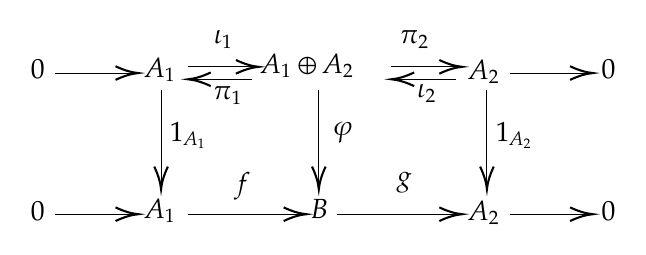
\begin{tikzpicture}[x=0.75pt,y=0.75pt,yscale=-1,xscale=1]
%uncomment if require: \path (0,476); %set diagram left start at 0, and has height of 476

%Straight Lines [id:da22573280049285005] 
\draw    (134,224) -- (172,224) ;
\draw [shift={(174,224)}, rotate = 180] [color={rgb, 255:red, 0; green, 0; blue, 0 }  ][line width=0.75]    (10.93,-3.29) .. controls (6.95,-1.4) and (3.31,-0.3) .. (0,0) .. controls (3.31,0.3) and (6.95,1.4) .. (10.93,3.29)   ;
%Straight Lines [id:da5007083409135236] 
\draw    (198,221) -- (230,221) ;
\draw [shift={(232,221)}, rotate = 180] [color={rgb, 255:red, 0; green, 0; blue, 0 }  ][line width=0.75]    (10.93,-3.29) .. controls (6.95,-1.4) and (3.31,-0.3) .. (0,0) .. controls (3.31,0.3) and (6.95,1.4) .. (10.93,3.29)   ;
%Straight Lines [id:da49627755138453633] 
\draw    (296,221) -- (328,221) ;
\draw [shift={(330,221)}, rotate = 180] [color={rgb, 255:red, 0; green, 0; blue, 0 }  ][line width=0.75]    (10.93,-3.29) .. controls (6.95,-1.4) and (3.31,-0.3) .. (0,0) .. controls (3.31,0.3) and (6.95,1.4) .. (10.93,3.29)   ;
%Straight Lines [id:da7229825431747845] 
\draw    (353,224) -- (391,224) ;
\draw [shift={(393,224)}, rotate = 180] [color={rgb, 255:red, 0; green, 0; blue, 0 }  ][line width=0.75]    (10.93,-3.29) .. controls (6.95,-1.4) and (3.31,-0.3) .. (0,0) .. controls (3.31,0.3) and (6.95,1.4) .. (10.93,3.29)   ;
%Straight Lines [id:da9219190287457819] 
\draw    (185,232) -- (185,278) ;
\draw [shift={(185,280)}, rotate = 270] [color={rgb, 255:red, 0; green, 0; blue, 0 }  ][line width=0.75]    (10.93,-3.29) .. controls (6.95,-1.4) and (3.31,-0.3) .. (0,0) .. controls (3.31,0.3) and (6.95,1.4) .. (10.93,3.29)   ;
%Straight Lines [id:da4241610695219813] 
\draw    (261,232) -- (261,278) ;
\draw [shift={(261,280)}, rotate = 270] [color={rgb, 255:red, 0; green, 0; blue, 0 }  ][line width=0.75]    (10.93,-3.29) .. controls (6.95,-1.4) and (3.31,-0.3) .. (0,0) .. controls (3.31,0.3) and (6.95,1.4) .. (10.93,3.29)   ;
%Straight Lines [id:da5742073517286415] 
\draw    (342,232) -- (342,278) ;
\draw [shift={(342,280)}, rotate = 270] [color={rgb, 255:red, 0; green, 0; blue, 0 }  ][line width=0.75]    (10.93,-3.29) .. controls (6.95,-1.4) and (3.31,-0.3) .. (0,0) .. controls (3.31,0.3) and (6.95,1.4) .. (10.93,3.29)   ;
%Straight Lines [id:da062379905314969175] 
\draw    (134,292) -- (172,292) ;
\draw [shift={(174,292)}, rotate = 180] [color={rgb, 255:red, 0; green, 0; blue, 0 }  ][line width=0.75]    (10.93,-3.29) .. controls (6.95,-1.4) and (3.31,-0.3) .. (0,0) .. controls (3.31,0.3) and (6.95,1.4) .. (10.93,3.29)   ;
%Straight Lines [id:da2958761370037739] 
\draw    (198,292) -- (253,292) ;
\draw [shift={(255,292)}, rotate = 180] [color={rgb, 255:red, 0; green, 0; blue, 0 }  ][line width=0.75]    (10.93,-3.29) .. controls (6.95,-1.4) and (3.31,-0.3) .. (0,0) .. controls (3.31,0.3) and (6.95,1.4) .. (10.93,3.29)   ;
%Straight Lines [id:da3240286217569581] 
\draw    (270,292) -- (328,292) ;
\draw [shift={(330,292)}, rotate = 180] [color={rgb, 255:red, 0; green, 0; blue, 0 }  ][line width=0.75]    (10.93,-3.29) .. controls (6.95,-1.4) and (3.31,-0.3) .. (0,0) .. controls (3.31,0.3) and (6.95,1.4) .. (10.93,3.29)   ;
%Straight Lines [id:da0337697350918047] 
\draw    (353,292) -- (391,292) ;
\draw [shift={(393,292)}, rotate = 180] [color={rgb, 255:red, 0; green, 0; blue, 0 }  ][line width=0.75]    (10.93,-3.29) .. controls (6.95,-1.4) and (3.31,-0.3) .. (0,0) .. controls (3.31,0.3) and (6.95,1.4) .. (10.93,3.29)   ;
%Straight Lines [id:da3278595213426152] 
\draw    (229,227) -- (200,227) ;
\draw [shift={(198,227)}, rotate = 360] [color={rgb, 255:red, 0; green, 0; blue, 0 }  ][line width=0.75]    (10.93,-3.29) .. controls (6.95,-1.4) and (3.31,-0.3) .. (0,0) .. controls (3.31,0.3) and (6.95,1.4) .. (10.93,3.29)   ;
%Straight Lines [id:da9309139657319496] 
\draw    (327,227) -- (298,227) ;
\draw [shift={(296,227)}, rotate = 360] [color={rgb, 255:red, 0; green, 0; blue, 0 }  ][line width=0.75]    (10.93,-3.29) .. controls (6.95,-1.4) and (3.31,-0.3) .. (0,0) .. controls (3.31,0.3) and (6.95,1.4) .. (10.93,3.29)   ;

% Text Node
\draw (121,216.4) node [anchor=north west][inner sep=0.75pt]    {$0$};
% Text Node
\draw (176,215.4) node [anchor=north west][inner sep=0.75pt]    {$A_{1}$};
% Text Node
\draw (232,213.4) node [anchor=north west][inner sep=0.75pt]    {$A_{1} \oplus A_{2}$};
% Text Node
\draw (332,216.4) node [anchor=north west][inner sep=0.75pt]    {$A_{2}$};
% Text Node
\draw (396,216.4) node [anchor=north west][inner sep=0.75pt]    {$0$};
% Text Node
\draw (188,246.4) node [anchor=north west][inner sep=0.75pt]    {$1_{A_{1}}$};
% Text Node
\draw (267,246.4) node [anchor=north west][inner sep=0.75pt]    {$\varphi $};
% Text Node
\draw (345,246.4) node [anchor=north west][inner sep=0.75pt]    {$1_{A_{2}}$};
% Text Node
\draw (121,284.4) node [anchor=north west][inner sep=0.75pt]    {$0$};
% Text Node
\draw (176,283.4) node [anchor=north west][inner sep=0.75pt]    {$A_{1}$};
% Text Node
\draw (256,283.4) node [anchor=north west][inner sep=0.75pt]    {$B$};
% Text Node
\draw (332,284.4) node [anchor=north west][inner sep=0.75pt]    {$A_{2}$};
% Text Node
\draw (396,284.4) node [anchor=north west][inner sep=0.75pt]    {$0$};
% Text Node
\draw (219,270.4) node [anchor=north west][inner sep=0.75pt]    {$f$};
% Text Node
\draw (297,270.4) node [anchor=north west][inner sep=0.75pt]    {$g$};
% Text Node
\draw (209,202.4) node [anchor=north west][inner sep=0.75pt]    {$\iota _{1}$};
% Text Node
\draw (299,202.4) node [anchor=north west][inner sep=0.75pt]    {$\pi _{2}$};
% Text Node
\draw (209,229.4) node [anchor=north west][inner sep=0.75pt]    {$\pi _{1}$};
% Text Node
\draw (307,228.4) node [anchor=north west][inner sep=0.75pt]    {$\iota _{2}$};


\end{tikzpicture}
\end{center}
we define $h:A_2\to B$ to be $\varphi\iota_2$ and $k:B\to A$ to be $\pi_1\varphi^{-1}$, then it is easy to verify that $h$ and $k$ satisfy the conditions.
\end{proof}
\begin{center}
\begin{large}
    \textbf{Exercises for 5.1}
\end{large}
\end{center}
Note that $R$ is a ring.
\begin{problem}\em
If $A$ is an abelian group and $n>0$ an integer such that $na=0$ for all $a\in A$, then $A$ is a unitary $\mathbb{Z}_n$-module, with the action of $\mathbb{Z}_n$ on $A$ given by $\overline{k}a=ka$, there $k\in\mathbb{Z}$ and $k\mapsto\overline{k}\in\mathbb{Z}_n$ under the canonical projection $\mathbb{Z}\to\mathbb{Z}_n$.
\end{problem}
\begin{proof}
Let $a,b\in A$ and $\overline{r},\overline{s}\in\mathbb{Z}_n$, then clearly $(\overline{r})(a+b)=r(a+b)=ra+rb$, $(\overline{r}+\overline{s})a=(r+s)a=ra+sa$ and $(\overline{r}\overline{s})a=(rs)a=r(sa)$, which showed that $A$ is a $\mathbb{Z}_n$-module.
\end{proof}
\begin{problem}\em
Let $f:A\to B$ be an $R$-module homomorphism.\par
(a) $f$ is a monomorphism if and only if for every pair of $R$-module homomorphisms $g,h:D\to A$ such that $fg=fh$, we have $g=h$.\par
(b) $f$ is an epimorphism if and only if for every pair of $R$-module homomorphisms $k,t:B\to C$ such that $kf=tf$, we have $k=t$.
\end{problem}
\begin{proof}
(a) Suppose $f$ is a monomorphism and $fg=fh$. Then for all $x\in D$ we have $fg(x)=fh(x)$, whence $f[g(x)-g(x)]=0$. Therefore $g(x)-h(x)\in\mathrm{Ker}f$. Since $f$ is a monomorphism, we obtain $g(x)-h(x)=0$, whence $g(x)=h(x)$. Conversely, let $D=\mathrm{Ker}f$, $g$ the inclusion map and $h$ the zero map. Then for all $x\in\mathrm{Ker}f$ we have $fg(x)=fh(x)$, whence $fg=fh$. Then by the assumption we conclude that $g=h$, which shows that $\mathrm{Ker}f=0$.\par
(b) Suppose $f$ is an epimorphism and $kf=tf$. Then for all $b\in B$ there exists some $a\in A$ such that $f(a)=b$, and hence $kf(a)=tf(a)$. Since this is true for all $b\in B$, we have $k=f$. Conversely, let $k$ be the canonical epimorphism $B\to B/\mathrm{Im}f$ and $t$ the zero map. Therefore for all $a\in A$ we have $kf(a)=tf(a)=0$, whence $k=t$. This implies $B/\mathrm{Im}f=0$, which is $B=\mathrm{Im}f$ and $f$ an epimorphism.
\end{proof}
\begin{problem}\em
Let $I$ be a left ideal of a ring $R$ and $A$ an $R$-module.\par
(a) If $S$ is a nonempty subset of $A$, then $IS=\left\{\sum_{i=1}^nr_ia_i:n\in\mathbb{N}_+,r_i\in I,a_i\in S\right\}$ is a submodule of $A$. Note that if $S=\{a\}$, then $IS=Ia=\{ra:r\in I\}$.\par
(b) If $I$ is a two-sided ideal, then $A/IA$ is an $R/I$-module with the action of $R/I$ given by $(r+I)(a+IA)=ra+IA$.
\end{problem}
\begin{proof}
(a) Clearly $IS$ is an additive abelian group. Now for all $r\in R$, we have $r\cdot r_ia_i\in IS$ since $I$ is a left ideal of $R$, whence $IS$ is a submodule of $A$.\par
(b) Clearly $A/IA$ is an abelian group. Suppose $r+I$, $s+I\in R/I$ and $a+IA$, $b+IA\in A/IA$, we have $(r+s+I)(a+IA)=(r+s)a+IA=(r+IA)+(s+IA)$, $(r+I)(a+b+IA)=r(a+b)+IA=(ra+IA)+(rb+IA)$ and $((r+I)(s+I))(a+IA)=(r+I)((s+I)(a+IA))$, therefore $A/IA$ is an $R/I$-module with the action of $R/I$ given by $(r+I)(a+IA)=ra+IA$.
\end{proof}
\begin{problem}\em
If $R$ has an identity, then every unitary cyclic $R$-module is isomorphic to an $R$-module of the form $R/J$, where $J$ is a left ideal of $R$.
\end{problem}
\begin{proof}
We define $J=\{x\in A:xa=0\}$. We first show that $J$ is a left ideal of $R$. Suppose $r\in R$, then $rJ\subset J$. Next, define the action of $R$ by multiplication, then $R/J$ is easily seen an $R$-module. Now suppose $A$ is cyclic, i.e., $A=\{ra:r\in R\}$, then define a homomorphism $f:R\to A$ given by $r\mapsto ra$, clearly $f$ is an epimorphism. Therefore by the First Isomorphism Theorem we obtain $A/\mathrm{Ker}f=A/J\cong R$, which finished the proof.
\end{proof}
\begin{problem}\em
If $R$ has an identity, then a nonzero unitary $R$-module $A$ is \textbf{simple} if and only if its submodules are $0$ and $A$.\par
(a) Every simple $R$-module is cyclic.\par
(b) If $A$ is simple every $R$-module endomorphism is either the zero map or an isomorphism.
\end{problem}
\begin{proof}
(a) Suppose $A$ is a simple $R$-module, then for all $a\in A$, we have $ra\in A$ for all $r\in R$, whence $A=Ra$ and it is cyclic.\par
(b) Suppose $f\in\mathrm{End}_RA$, then since $\mathrm{Ker}f$ and $\mathrm{Im}f$ are submodules of $A$, we have $\mathrm{Ker}f=0$ or $\mathrm{Ker}f=A$ (the same is true for $\mathrm{Im}f$). Suppose $x\in R$ and $x\ne 0$. If $x\in\mathrm{Ker}f$, then $\mathrm{Ker}f=A$, whence $f$ is zero map. If $x\notin\mathrm{Ker}f$, then $\mathrm{Ker}f=0$, and hence $f$ is monomorphism. Since $f(x)\ne 0$, it forces $\mathrm{Im}f=A$ and hence $f$ is an isomorphism.
\end{proof}
\begin{problem}\em
A finitely generated $R$-module need not be finitely generated abelian group.
\end{problem}
\begin{proof}
Consider $\mathbb{Q}$. Clearly $\mathbb{Q}$ is a finitely generated $\mathbb{Q}$-module, however, $\mathbb{Q}$ is not a finitely generated abelian group.
\end{proof}
\begin{problem}\em
(a) If $A$ and $B$ are $R$-modules, then the set $\mathrm{Hom}_R(A,B)$ of all $R$-module homomorphisms $A\to B$ is an abelian group with $f+g$ given on $a\in A$ by $(f+g)(a)=f(a)+g(a)\in B$. The identity element is the zero map.\par
(b) $\mathrm{End}_RA=\mathrm{Hom}_R(A,A)$ is a ring with identity, where multiplication is composition of functions. $\mathrm{End}_RA$ is called the \textbf{endomorphism ring} of $A$.\par
(c) $A$ is a left $\mathrm{End}_RA$-module with $fa$ defined to be $f(a)$, $a\in A$, $f\in\mathrm{End}_RA$.
\end{problem}
\begin{proof}
(a) Observe that $(f+g)(x)=f(x)+g(x)=g(x)+f(x)=(g+f)(x)$ for all $x\in A$.\par
(b) By (a) we have $(\mathrm{End}_RA,+)$ is an abelian group. Now we show that $\mathrm{End}_RA$ is a ring. Observe that $(f+g)h=fh+gh$, $h(f+g)=hf+hg$, and $f(gh)=(fg)h$, we have $\mathrm{End}_RA$ is a ring. The identity of $\mathrm{End}_RA$ is $1_{A\to A}$.\par
(c) Suppose $f,g\in\mathrm{End}_RA$ and $a,b\in A$. Then $f(a+b)=f(a)+f(b)$, $(f+g)(a)=f(a)+g(a)$ and $f(g(a))=(fg)(a)$, whence $A$ is an $\mathrm{End}_RA$-module.
\end{proof}
\begin{problem}\em
If $f:A\to A$ is an $R$-module homomorphism such that $ff=f$, then $A=\mathrm{Ker}f\oplus\mathrm{Im}f$.
\end{problem}
\begin{proof}
We consider the short exact sequence: 
$$
0\hookrightarrow \mathrm{Ker}f\longrightarrow A\overset{f}{\longrightarrow}\mathrm{Im}f\longrightarrow 0,
$$
suppose $f(x)=y$, then $ff(x)=f(y)=f(x)=y$, whence $ff\mid_{\mathrm{Im}f}=1_{\mathrm{Im}f}$. Therefore by Theorem 5.12 we have the following diagram 
\begin{center}


\tikzset{every picture/.style={line width=0.75pt}} %set default line width to 0.75pt        

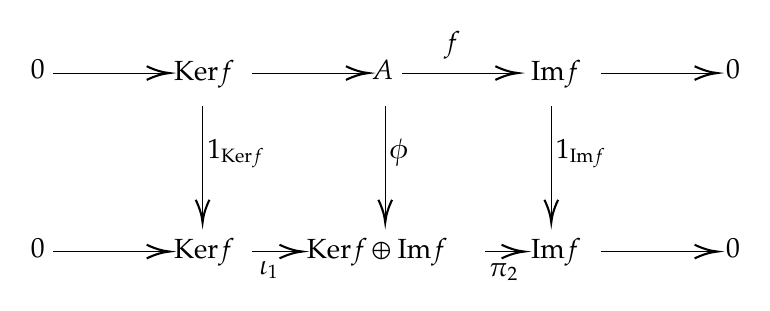
\begin{tikzpicture}[x=0.75pt,y=0.75pt,yscale=-1,xscale=1]
%uncomment if require: \path (0,476); %set diagram left start at 0, and has height of 476

%Straight Lines [id:da11523337004831591] 
\draw    (136,200) -- (190,200) ;
\draw [shift={(192,200)}, rotate = 180] [color={rgb, 255:red, 0; green, 0; blue, 0 }  ][line width=0.75]    (10.93,-3.29) .. controls (6.95,-1.4) and (3.31,-0.3) .. (0,0) .. controls (3.31,0.3) and (6.95,1.4) .. (10.93,3.29)   ;
%Straight Lines [id:da7904190363259922] 
\draw    (232,200) -- (286,200) ;
\draw [shift={(288,200)}, rotate = 180] [color={rgb, 255:red, 0; green, 0; blue, 0 }  ][line width=0.75]    (10.93,-3.29) .. controls (6.95,-1.4) and (3.31,-0.3) .. (0,0) .. controls (3.31,0.3) and (6.95,1.4) .. (10.93,3.29)   ;
%Straight Lines [id:da587990758726602] 
\draw    (304,200) -- (358,200) ;
\draw [shift={(360,200)}, rotate = 180] [color={rgb, 255:red, 0; green, 0; blue, 0 }  ][line width=0.75]    (10.93,-3.29) .. controls (6.95,-1.4) and (3.31,-0.3) .. (0,0) .. controls (3.31,0.3) and (6.95,1.4) .. (10.93,3.29)   ;
%Straight Lines [id:da9885626053073777] 
\draw    (400,200) -- (454,200) ;
\draw [shift={(456,200)}, rotate = 180] [color={rgb, 255:red, 0; green, 0; blue, 0 }  ][line width=0.75]    (10.93,-3.29) .. controls (6.95,-1.4) and (3.31,-0.3) .. (0,0) .. controls (3.31,0.3) and (6.95,1.4) .. (10.93,3.29)   ;
%Straight Lines [id:da3308579976843522] 
\draw    (136,286) -- (190,286) ;
\draw [shift={(192,286)}, rotate = 180] [color={rgb, 255:red, 0; green, 0; blue, 0 }  ][line width=0.75]    (10.93,-3.29) .. controls (6.95,-1.4) and (3.31,-0.3) .. (0,0) .. controls (3.31,0.3) and (6.95,1.4) .. (10.93,3.29)   ;
%Straight Lines [id:da6671524047453168] 
\draw    (232,286) -- (254,286) ;
\draw [shift={(256,286)}, rotate = 180] [color={rgb, 255:red, 0; green, 0; blue, 0 }  ][line width=0.75]    (10.93,-3.29) .. controls (6.95,-1.4) and (3.31,-0.3) .. (0,0) .. controls (3.31,0.3) and (6.95,1.4) .. (10.93,3.29)   ;
%Straight Lines [id:da4339888772828562] 
\draw    (344,286) -- (361,286) ;
\draw [shift={(363,286)}, rotate = 180] [color={rgb, 255:red, 0; green, 0; blue, 0 }  ][line width=0.75]    (10.93,-3.29) .. controls (6.95,-1.4) and (3.31,-0.3) .. (0,0) .. controls (3.31,0.3) and (6.95,1.4) .. (10.93,3.29)   ;
%Straight Lines [id:da021376580311138982] 
\draw    (400,286) -- (454,286) ;
\draw [shift={(456,286)}, rotate = 180] [color={rgb, 255:red, 0; green, 0; blue, 0 }  ][line width=0.75]    (10.93,-3.29) .. controls (6.95,-1.4) and (3.31,-0.3) .. (0,0) .. controls (3.31,0.3) and (6.95,1.4) .. (10.93,3.29)   ;
%Straight Lines [id:da49203458496172336] 
\draw    (208,216) -- (208,270) ;
\draw [shift={(208,272)}, rotate = 270] [color={rgb, 255:red, 0; green, 0; blue, 0 }  ][line width=0.75]    (10.93,-3.29) .. controls (6.95,-1.4) and (3.31,-0.3) .. (0,0) .. controls (3.31,0.3) and (6.95,1.4) .. (10.93,3.29)   ;
%Straight Lines [id:da12466324878794266] 
\draw    (376,216) -- (376,270) ;
\draw [shift={(376,272)}, rotate = 270] [color={rgb, 255:red, 0; green, 0; blue, 0 }  ][line width=0.75]    (10.93,-3.29) .. controls (6.95,-1.4) and (3.31,-0.3) .. (0,0) .. controls (3.31,0.3) and (6.95,1.4) .. (10.93,3.29)   ;
%Straight Lines [id:da19403386152219593] 
\draw    (296,216) -- (296,270) ;
\draw [shift={(296,272)}, rotate = 270] [color={rgb, 255:red, 0; green, 0; blue, 0 }  ][line width=0.75]    (10.93,-3.29) .. controls (6.95,-1.4) and (3.31,-0.3) .. (0,0) .. controls (3.31,0.3) and (6.95,1.4) .. (10.93,3.29)   ;

% Text Node
\draw (124,192.4) node [anchor=north west][inner sep=0.75pt]    {$0$};
% Text Node
\draw (193,192.4) node [anchor=north west][inner sep=0.75pt]    {$\mathrm{Ker} f$};
% Text Node
\draw (289,192.4) node [anchor=north west][inner sep=0.75pt]    {$A$};
% Text Node
\draw (365,192.4) node [anchor=north west][inner sep=0.75pt]    {$\mathrm{Im} f$};
% Text Node
\draw (459,192.4) node [anchor=north west][inner sep=0.75pt]    {$0$};
% Text Node
\draw (124,278.4) node [anchor=north west][inner sep=0.75pt]    {$0$};
% Text Node
\draw (193,278.4) node [anchor=north west][inner sep=0.75pt]    {$\mathrm{Ker} f$};
% Text Node
\draw (257,278.4) node [anchor=north west][inner sep=0.75pt]    {$\mathrm{Ker} f\oplus \mathrm{Im} f$};
% Text Node
\draw (365,278.4) node [anchor=north west][inner sep=0.75pt]    {$\mathrm{Im} f$};
% Text Node
\draw (459,278.4) node [anchor=north west][inner sep=0.75pt]    {$0$};
% Text Node
\draw (323,178.4) node [anchor=north west][inner sep=0.75pt]    {$f$};
% Text Node
\draw (234,289.4) node [anchor=north west][inner sep=0.75pt]    {$\iota _{1}$};
% Text Node
\draw (345,290.4) node [anchor=north west][inner sep=0.75pt]    {$\pi _{2}$};
% Text Node
\draw (297,230.4) node [anchor=north west][inner sep=0.75pt]    {$\phi $};
% Text Node
\draw (377,230.4) node [anchor=north west][inner sep=0.75pt]    {$1_{\mathrm{Im} f}{}$};
% Text Node
\draw (209,230.4) node [anchor=north west][inner sep=0.75pt]    {$1_{\mathrm{Ker} f}$};


\end{tikzpicture}
\end{center}
is commutative, and hence $\phi$ is an isomorphism. Therefore $A\cong\mathrm{Ker}f\oplus\mathrm{Im}f$.
\end{proof}
\begin{problem}\em
Let $A,A_1,\cdots,A_n$ be $R$-modules. Then $A\cong A_1\oplus A_2\oplus\cdots\oplus A_n$ if and only if for each $i=1,2,\cdots,n$ there is an $R$-module homomorphism $\varphi_i:A\to A$ such that $\mathrm{Im}\varphi_i\cong A_i$, $\varphi_i\varphi_j=0$ for $i\ne j$ and $\varphi_1+\varphi_2+\cdots+\varphi_n=1_A$.
\end{problem}
\begin{proof}
Suppose $A\cong A_1\oplus\cdots\oplus A_n$, then let $\varphi_i=\iota_i\circ\pi_i$. Conversely, given $\{\varphi_i\}$, we first show that $\varphi_i\circ\varphi_i=\varphi_i$. Observe that $\varphi_1+\cdots+\varphi_n=1_A$, we have $\varphi_i\circ\varphi_1+\cdots+\varphi_i\circ\varphi_i+\cdots+\varphi_i\circ\varphi_n=\varphi_i$. However $\varphi_i\circ\varphi_j=0$ when $i\ne j$, we have $\varphi_i\circ\varphi_i=\varphi_i$. Now define $\psi_i=\varphi_i\mid_{\mathrm{Im}\varphi_i}$ and apply Theorem 5.9.
\end{proof}
\begin{problem}\em
(a) If $A$ is a module over a commutative ring $R$ and $a\in A$, then $\mathcal{O}_a=\{r\in R:ra=0\}$ is an ideal of $R$. If $\mathcal{O}_a\ne 0$, $a$ is said to be a \textbf{torsion element} of $A$.\par
(b) If $R$ is an integral domain, then the set $T(A)$ of all torsion elements of $A$ is a submodule of $A$.($T(A)$ is called the \textbf{torsion submodule}.)\par
(c) Show that (b) may be false if $R$ is not an integral domain.\par
In (d)-(f) $R$ is an integral domain.\par
(d) If $f:A\to B$ is an $R$-module homomorphism, then $f(T(A))\subset T(B)$, hence the restriction $f_T$ of $f$ to $T(A)$ is an $R$-module homomorphism $T(A)\to T(B)$.\par
(e) If $0\longrightarrow A\overset{f}{\longrightarrow}B\overset{g}{\longrightarrow}C$ is an exact sequence of $R$-modules, then so is $0\longrightarrow T\left( A \right) \overset{f_T}{\longrightarrow}T\left( B \right) \overset{g_T}{\longrightarrow}T(C)$.\par
(f) If $g:B\to C$ is an $R$-module epimorphism, then $g_T:T(B)\to T(C)$ need not be an epimorphism.
\end{problem}
\begin{proof}
(a) Let $r_0\in R$, then for all $ra\in\mathcal{O}_a$, we have $r_0ra=0$, hence $r_0r\in\mathcal{O}_a$. Since $R$ is commutative, we conclude that $\mathcal{O}_a$ is an ideal of $R$.\par
(b) We first show that $T(A)$ is a additive subgroup of $A$. Let $a,b\in T(A)$, then $\mathcal{O}_a$ and $\mathcal{O}_b$ are both nonempty. Let $r_a\in\mathcal{O}_a$ and $r_b\in\mathcal{O}_b$, then $r_ar_b(a+b)=0$, whence $a+b\in T(A)$. Note that $r_ar_b\ne 0$ since $r_a\ne 0$, $r_b\ne 0$, and $R$ is an integral domain. Now suppose $r_0\in R$, then $r_0ra=0$, hence $T(A)$ is a submodule of $A$.\par
(c) Consider the $\mathbb{Z}/12\mathbb{Z}$-module $\mathbb{Z}/12\mathbb{Z}$. Since $\overline{3}\cdot\overline{4}=\overline{2}\cdot\overline{6}=\overline{0}$, we have $\overline{4},\overline{6}\in T(\mathbb{Z}/12\mathbb{Z})$. However $\overline{4}+\overline{6}=\overline{10}\notin T(\mathbb{Z}/12\mathbb{Z})$.\par
(d) Let $a\in T(A)$, then there exists some nonzero $r\in R$ such that $ra=0$. Therefore $f(ra)=rf(a)=0$, whence $f(a)\in T(B)$. Therefore $f(T(A))\subset T(B)$.\par
(e) Since $0\longrightarrow A\overset{f}{\longrightarrow}B\overset{g}{\longrightarrow}C$ is an exact sequence of $R$-modules, then $\mathrm{Im}f=\mathrm{Ker}g$. Now we show that $\mathrm{Im}f_T=\mathrm{Ker}g_T$. Let $b\in\mathrm{Im}f_T$, then $b\in\mathrm{Im}f$ and hence $b\in\mathrm{Ker}g$. Since $b\in T(B)$ we have $g_T(b)=0$, whence $b\in\mathrm{Ker}g_T$. This shows $\mathrm{Im}f_T\subset\mathrm{Ker}g_T$. For the converse inequality, suppose $b\in\mathrm{Ker}g_T$. Then $b\in\mathrm{Ker}g=\mathrm{Im}f$, therefore there exists some $a\in A$ such that $f(a)=b$. Since $b\in T(B)$, there exists some nonzero $r\in R$ such that $rb=0$. Consider $f(ra)=rf(a)=rb=0$, we have $ra\in\mathrm{Ker}f$. However $\mathrm{Ker}f=0$, therefore $a\in T(A)$, and the proof is finished.\par
(f) Consider $\mathbb{Z}$ and $\mathbb{Z}/4\mathbb{Z}$ as $\mathbb{Z}$-modules, define $g:\mathbb{Z}\mapsto\mathbb{Z}/4\mathbb{Z}$ as $n\mapsto n\ \mathrm{mod}4$.
\end{proof}
\begin{problem}\em
Let 
\begin{center}


\tikzset{every picture/.style={line width=0.75pt}} %set default line width to 0.75pt        

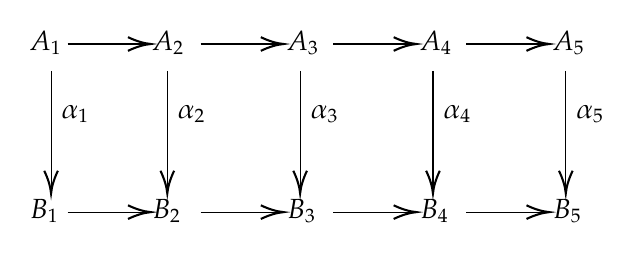
\begin{tikzpicture}[x=0.75pt,y=0.75pt,yscale=-1,xscale=1]
%uncomment if require: \path (0,476); %set diagram left start at 0, and has height of 476

%Straight Lines [id:da2968650742386445] 
\draw    (184,200) -- (222,200) ;
\draw [shift={(224,200)}, rotate = 180] [color={rgb, 255:red, 0; green, 0; blue, 0 }  ][line width=0.75]    (10.93,-3.29) .. controls (6.95,-1.4) and (3.31,-0.3) .. (0,0) .. controls (3.31,0.3) and (6.95,1.4) .. (10.93,3.29)   ;
%Straight Lines [id:da3087931668138173] 
\draw    (248,200) -- (286,200) ;
\draw [shift={(288,200)}, rotate = 180] [color={rgb, 255:red, 0; green, 0; blue, 0 }  ][line width=0.75]    (10.93,-3.29) .. controls (6.95,-1.4) and (3.31,-0.3) .. (0,0) .. controls (3.31,0.3) and (6.95,1.4) .. (10.93,3.29)   ;
%Straight Lines [id:da43900145473204155] 
\draw    (312,200) -- (350,200) ;
\draw [shift={(352,200)}, rotate = 180] [color={rgb, 255:red, 0; green, 0; blue, 0 }  ][line width=0.75]    (10.93,-3.29) .. controls (6.95,-1.4) and (3.31,-0.3) .. (0,0) .. controls (3.31,0.3) and (6.95,1.4) .. (10.93,3.29)   ;
%Straight Lines [id:da7713018854398284] 
\draw    (376,200) -- (414,200) ;
\draw [shift={(416,200)}, rotate = 180] [color={rgb, 255:red, 0; green, 0; blue, 0 }  ][line width=0.75]    (10.93,-3.29) .. controls (6.95,-1.4) and (3.31,-0.3) .. (0,0) .. controls (3.31,0.3) and (6.95,1.4) .. (10.93,3.29)   ;
%Straight Lines [id:da7107268582024568] 
\draw    (184,281) -- (222,281) ;
\draw [shift={(224,281)}, rotate = 180] [color={rgb, 255:red, 0; green, 0; blue, 0 }  ][line width=0.75]    (10.93,-3.29) .. controls (6.95,-1.4) and (3.31,-0.3) .. (0,0) .. controls (3.31,0.3) and (6.95,1.4) .. (10.93,3.29)   ;
%Straight Lines [id:da024645825848374825] 
\draw    (248,281) -- (286,281) ;
\draw [shift={(288,281)}, rotate = 180] [color={rgb, 255:red, 0; green, 0; blue, 0 }  ][line width=0.75]    (10.93,-3.29) .. controls (6.95,-1.4) and (3.31,-0.3) .. (0,0) .. controls (3.31,0.3) and (6.95,1.4) .. (10.93,3.29)   ;
%Straight Lines [id:da01920398666668821] 
\draw    (312,281) -- (350,281) ;
\draw [shift={(352,281)}, rotate = 180] [color={rgb, 255:red, 0; green, 0; blue, 0 }  ][line width=0.75]    (10.93,-3.29) .. controls (6.95,-1.4) and (3.31,-0.3) .. (0,0) .. controls (3.31,0.3) and (6.95,1.4) .. (10.93,3.29)   ;
%Straight Lines [id:da7055791271948879] 
\draw    (376,281) -- (414,281) ;
\draw [shift={(416,281)}, rotate = 180] [color={rgb, 255:red, 0; green, 0; blue, 0 }  ][line width=0.75]    (10.93,-3.29) .. controls (6.95,-1.4) and (3.31,-0.3) .. (0,0) .. controls (3.31,0.3) and (6.95,1.4) .. (10.93,3.29)   ;
%Straight Lines [id:da7896973425174743] 
\draw    (176,213) -- (176,270) ;
\draw [shift={(176,272)}, rotate = 270] [color={rgb, 255:red, 0; green, 0; blue, 0 }  ][line width=0.75]    (10.93,-3.29) .. controls (6.95,-1.4) and (3.31,-0.3) .. (0,0) .. controls (3.31,0.3) and (6.95,1.4) .. (10.93,3.29)   ;
%Straight Lines [id:da6414063846519429] 
\draw    (232,213) -- (232,270) ;
\draw [shift={(232,272)}, rotate = 270] [color={rgb, 255:red, 0; green, 0; blue, 0 }  ][line width=0.75]    (10.93,-3.29) .. controls (6.95,-1.4) and (3.31,-0.3) .. (0,0) .. controls (3.31,0.3) and (6.95,1.4) .. (10.93,3.29)   ;
%Straight Lines [id:da857172487299223] 
\draw    (296,213) -- (296,270) ;
\draw [shift={(296,272)}, rotate = 270] [color={rgb, 255:red, 0; green, 0; blue, 0 }  ][line width=0.75]    (10.93,-3.29) .. controls (6.95,-1.4) and (3.31,-0.3) .. (0,0) .. controls (3.31,0.3) and (6.95,1.4) .. (10.93,3.29)   ;
%Straight Lines [id:da5314329341376476] 
\draw    (360,213) -- (360,270) ;
\draw [shift={(360,272)}, rotate = 270] [color={rgb, 255:red, 0; green, 0; blue, 0 }  ][line width=0.75]    (10.93,-3.29) .. controls (6.95,-1.4) and (3.31,-0.3) .. (0,0) .. controls (3.31,0.3) and (6.95,1.4) .. (10.93,3.29)   ;
%Straight Lines [id:da13029719909082838] 
\draw    (424,213) -- (424,270) ;
\draw [shift={(424,272)}, rotate = 270] [color={rgb, 255:red, 0; green, 0; blue, 0 }  ][line width=0.75]    (10.93,-3.29) .. controls (6.95,-1.4) and (3.31,-0.3) .. (0,0) .. controls (3.31,0.3) and (6.95,1.4) .. (10.93,3.29)   ;

% Text Node
\draw (165,192.4) node [anchor=north west][inner sep=0.75pt]    {$A_{1}$};
% Text Node
\draw (224,192.4) node [anchor=north west][inner sep=0.75pt]    {$A_{2}$};
% Text Node
\draw (289,192.4) node [anchor=north west][inner sep=0.75pt]    {$A_{3}$};
% Text Node
\draw (353,192.4) node [anchor=north west][inner sep=0.75pt]    {$A_{4}$};
% Text Node
\draw (417,192.4) node [anchor=north west][inner sep=0.75pt]    {$A_{5}$};
% Text Node
\draw (165,273.4) node [anchor=north west][inner sep=0.75pt]    {$B_{1}$};
% Text Node
\draw (224,273.4) node [anchor=north west][inner sep=0.75pt]    {$B_{2}$};
% Text Node
\draw (289,273.4) node [anchor=north west][inner sep=0.75pt]    {$B_{3}$};
% Text Node
\draw (353,273.4) node [anchor=north west][inner sep=0.75pt]    {$B_{4}$};
% Text Node
\draw (417,273.4) node [anchor=north west][inner sep=0.75pt]    {$B_{5}$};
% Text Node
\draw (180,228.4) node [anchor=north west][inner sep=0.75pt]    {$\alpha _{1}$};
% Text Node
\draw (236,228.4) node [anchor=north west][inner sep=0.75pt]    {$\alpha _{2}$};
% Text Node
\draw (300,228.4) node [anchor=north west][inner sep=0.75pt]    {$\alpha _{3}$};
% Text Node
\draw (364,228.4) node [anchor=north west][inner sep=0.75pt]    {$\alpha _{4}$};
% Text Node
\draw (428,228.4) node [anchor=north west][inner sep=0.75pt]    {$\alpha _{5}$};


\end{tikzpicture}
\end{center}
be a commutative diagram of $R$-modules and $R$-module homomorphisms, with exact rows. Prove that \par
(a) $\alpha_1$ an epimorphism and $\alpha_2,\alpha_4$ monomorphisms implies $\alpha_3$ monomorphism.\par
(b) $\alpha_5$ an monomorphism and $\alpha_2,\alpha_4$ epimorphisms implies $\alpha_3$ epimorphism.
\end{problem}
\begin{proof}
We only show (a), and (b) may be proved in an analogous way. Suppose $\alpha_3(a_3)=0$, we now show that $a_3=0$. By the commutativity of the diagram we have 
$$
g_3\circ \alpha _3\left( a_3 \right) =\alpha _4\circ f_3\left( a_3 \right) \Rightarrow \alpha _3\in \mathrm{Ker}f_3=\mathrm{Im}f_2,
$$
therefore there exists some $a_2\in A_2$ such that $f_2(a_2)=0$. Again we have 
$$
\alpha _3\circ f_2\left( a_2 \right) =g_2\circ \alpha _2\left( a_2 \right) \Rightarrow \alpha _2\left( a_2 \right) \in \mathrm{Ker}g_2=\mathrm{Im}g_1,
$$
suppose $\alpha_2(a_2)=b_2$, there exists some $b_1\in B_1$ such that $g_1(b_1)=b_2$. Since $\alpha_1$ is an epimorphism, suppose $\alpha_1(a_1)=b_2$. Now that 
$$
g_2\circ g_1\circ \alpha _1\left( a_1 \right) =\alpha _3\circ f_2\circ f_1\left( a_1 \right) \Rightarrow a_1\in \mathrm{Ker}\alpha _2=0,
$$
whence $a_1=0$. Therefore $a_3=0$, and the prove is finished.
\end{proof}
\begin{problem}\em
(a) If $0\longrightarrow A\longrightarrow B\overset{f}{\longrightarrow}C\longrightarrow 0$ and $0\longrightarrow C\overset{g}{\longrightarrow}D\longrightarrow E\longrightarrow 0$ are short exact sequences of modules, then the sequence $0\longrightarrow A\longrightarrow B\overset{g\circ f}{\longrightarrow}D\longrightarrow E\longrightarrow 0$ is exact.\par
(b) Show that every exact sequence may be obtained by splicing together suitable short exact sequences as in (a).
\end{problem}
\begin{proof}
Suppose $\alpha:A\to B$ and $\beta:D\to E$, then by the exactness we have $\mathrm{Im}\alpha=\mathrm{Ker}f$ and $\mathrm{Im}g=\mathrm{Ker}\beta$. It suffices to show $\mathrm{Im}\alpha =\mathrm{Ker}g\circ f,\hspace{0.5cm}\mathrm{Im}g\circ f=\beta $. We first show $\mathrm{Ker}f=\mathrm{Ker}g\circ f$. Clearly $\mathrm{Ker}f\subset\mathrm{Ker}g\circ f$. Conversely, suppose $g\circ f(x)=0$, then $f(x)\in\mathrm{Ker}g$, whence $f(x)=0$. This implies $x\in\mathrm{Ker}f$. Since $\mathrm{Im}\alpha=\mathrm{Ker}f$, this shows that the sequence exact at $B$. Next we show that $\mathrm{Im}g\circ f=\mathrm{Ker}\beta$. Clearly $\mathrm{Im}g\circ f\subset\mathrm{Im}g$. However $\mathrm{Im}f=\mathrm{Ker}C=C$ implies that $f$ is an epimorphism, therefore $\mathrm{Im}g\circ f=\mathrm{Ker}\beta$, and the sequence is exact at $D$. An analogous argument may be made to show that (b) is true.
\end{proof}
\begin{problem}\em
If $f:A\to B$ and $g:B\to A$ are $R$-module homomorphisms such that $gf=1_A$, then $B=\mathrm{Im}f\oplus\mathrm{Ker}g$.
\end{problem}
\begin{proof}
Clearly the exact sequence $0\longrightarrow A\overset{f}{\longrightarrow}B\overset{g}{\longrightarrow}A\longrightarrow 0$ split, therefore it is equivalent to the sequence $0\longrightarrow A\overset{f}{\longrightarrow}\mathrm{Im}f\oplus \mathrm{Ker}g\overset{g}{\longrightarrow}A\longrightarrow 0$. In particular, $B\cong\mathrm{Im}f\oplus\mathrm{Ker}g$.
\end{proof}
\begin{problem}\em
Let $R$ be a ring and $R^{\mathrm{op}}$ is its opposite ring. If $A$ is a left [resp. right] $R$-module, then $A$ is a right [resp. left] $R^{\mathrm{op}}$-module such that $ra=ar$ for all $a\in A$, $r\in R$ and $r\in R^{\mathrm{op}}$.
\end{problem}
\begin{proof}
It suffices to verify the multiplication condition. Indeed, we observe that 
$$
a\left( r\circ s \right) =a\left( sr \right) =\left( as \right) r=r\circ \left( as \right) =\left( ar \right) \circ s,
$$
this finished the proof.
\end{proof}
\begin{problem}\em
(a) If $R$ has an identity and $A$ is an $R$-module, then there are submodules $B$ and $C$ of $A$ such that $B$ is unitary, $RC=0$ and $A=B\oplus C$.\par
(b) Let $A_1$ be another $R$-module, with $A_1=B_1\oplus C_1$ ($B_1$ binary, $RC_1=0$). If $f:A\to A_1$ is an $R$-module homomorphism then $f(B)\subset B_1$ and $f(C)\subset C_1$.\par
(c) If the map $f$ in (b) is an epimorphism [resp. isomorphism], then so are $f\mid_B$ and $f\mid_C$.
\end{problem}
\begin{proof}
(a) We define $B=\{1_Ra:a\in A\}$ and $C=\{a\in A:1_Ra=0\}$, then $B$ and $C$ are easily verified to be submodules of $A$ and $B$ unitary, $RC=0$. Note that for all $a\in A$, we have $a-1_Ra\in C$ and $B\cap C=0$, therefore $A=B\oplus C$.\par
(b) Suppose $f(B)\not\subset B_1$, then there exists some $b\in B$ such that $f(b)\in C$. Say $f(b)\ne 0$ or otherwise $f(b)\in B$. Then $f(1_Rb)=1_Rf(b)$. However $RC_1=0$, we obtain $f(b)=0$, a contradiction! Similarly we have $f(C)\subset C_1$.\par
(c) Suppose $(b_1,0)\in B_1\oplus C_1$. Since $f$ is an epimorphism and $f(B)\subset B_1$, there exists some $(b,0)\in B\oplus C$ such that $(b,0)\mapsto (b_1,0)$, therefore $f\mid_B$ is an epimorphism. Similarly we may show that $f\mid_C$ is an epimorphism, and the condition that $f$ is an isomorphism.
\end{proof}
\begin{problem}\em
Let $R$ be a ring without identity. Embed $R$ in a ring $S$ with identity and characteristic zero as in the proof of Theorem 4.10. Identity $R$ with its image in $S$.\par
(a) Show that every element of $S$ may be uniquely expressed in the form $r1_S+n1_S$, $r\in R, n\in\mathbb{Z}$.\par
(b) If $A$ is an $R$-module and $a\in A$, show that there is a unique $R$-module homomorphism $f:S\to A$ such that $f(1_S)=a$.
\end{problem}
\begin{proof}
(a) We use the notation in Theorem 4.10. Note that $1_S=(0,1)$, therefore for all $(r,n)\in S$, we have $(r,n)=(r,0)(0,1)+(0,n)(0,1)=r1_S+n1_S$.\par
(b) Let $f(r1_S+n1_S)=ra+na$, then it is a routine to check that $f$ satisfy the condition.
\end{proof}
\subsection{Free Modules and Vector Spaces}
In this section we will study the free objects in the category of modules over a ring. We first give some terminologies.\par
A subset $X$ of an $R$-module $A$ is said to be \textbf{linearly independent} provided that for distinct $x_1,\cdots,x_n\in X$ and $r_i\in R$, we have $r_1x_1+r_2x_2+\cdots+r_nx_n=0$ implies $r_i=0$ for every $i$. A set that is not linearly independent is said to be \textbf{linear dependent}. If $A$ is generated as an $R$-module by a set $Y$, then we say that $Y$ \textbf{spans} $A$. If $R$ has an identity and $A$ is unitary, $Y$ spans $A$ if and only if every element of $A$ may be written as a linear combination $r_1y_1+r_2y_2+\cdots+r_ny_n$, where $r_i\in R$ and $y_i\in Y$. A linearly independent subset of $A$ that spans $A$ is called a \textbf{basis} of $A$. Observe that the empty set is (vacuously) linearly independent and is a basis of the zero module.
\begin{theorem}
Let $R$ be a ring with identity. Then the following statement on a unitary $R$-module $F$ is equivalent:\par
(a) $F$ has a nonempty basis;\par
(b) $F$ is the internal direct sum of a family of cyclic $R$-modules, each of which is isomorphic as a left $R$-module to $R$;\par
(c) $F$ is an $R$-module isomorphic to a direct sum of copies of the left $R$-module $R$;\par
(d) $F$ is a free object in the category of unitary $R$-modules.
\end{theorem}
\begin{proof}
(a)$\Rightarrow$(b): Let $X$ be the basis of $F$. Let $x\in X$, then consider the homomorphism $r\mapsto rx$, $r\in R$. Clearly it is an epimorphism. If $rx=0$, then by linear independence we have $r=0$, whence $r\mapsto rx$ is a monomorphism, whence isomorphism. Note that for all $r\in R$ there exists some linear combination of elements in $X$, we have $F\cong\bigoplus_{x\in X}Rx\cong\bigoplus_{x\in X}R$.\par
(b)$\Rightarrow$(c): By (b) we have $R\cong\bigoplus_{x\in X}Rx$ and $Rx\cong R$. Therefore $R\cong\bigoplus_{x\in X}R_x$, where $R_x$ are isomorphic copies of $R$.\par
(c)$\Rightarrow$(a): Suppose $R\cong\bigoplus_{x\in X}R_x$. Take $\theta_x=\{r_i\}$, where $r_i=0$ for $i\ne x$ and $r_i=1_R$ for $i=x$. Then it is easy to verify that $\{\theta_x\}$ is a basis of $F$.\par
(a)$\Rightarrow$(d): Suppose $X$ is the basis of $F$, then for all $u\in F$, $u$ can be written in the form of $\sum_{x\in X}xr_x$ since $X$ spans $F$, here $r_x\in R$. Now define $\overline{f}$ by $\sum_{x\in X}xr_x\mapsto\sum_{x\in X}r_xf(x)$. We first show that $\overline{f}$ is well-defined. Suppose $u=\sum_{x\in X}xr_x=\sum_{x\in X}xs_x$, then $\sum_{x\in X}x(r_x-s_x)=0$, by linear independence we have $r_x=s_x$, whence $\overline{f}$ is well-defined. It is easy to verify that $\overline{f}$ is a homomorphism and $\overline{f}\iota=f$. Now suppose there is another $g$ such that $g\iota=f$. Then for all $x\in X$ we have $g(x)=g\iota(x)=f(x)=\overline{f}(x)$, and since $X$ spans $F$, we have $g=\overline{f}$.\par
(d)$\Rightarrow$(c): By (c)$\Rightarrow$(a) we know that there exists a basis $\{\theta_x\}$ of $F$. By (a)$\Rightarrow$(d) we know that $\bigoplus_{x\in\theta_x}R$ is a free object on the category of unitary $R$-modules. By the uniqueness of free objects in a category we finished the proof.
\end{proof}
\begin{note}\em
The statement (d) may be rephrased into the commutative diagram below: 
\begin{center}


\tikzset{every picture/.style={line width=0.75pt}} %set default line width to 0.75pt        

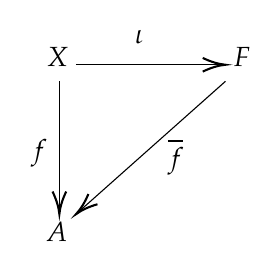
\begin{tikzpicture}[x=0.75pt,y=0.75pt,yscale=-1,xscale=1]
%uncomment if require: \path (0,476); %set diagram left start at 0, and has height of 476

%Straight Lines [id:da31374964360343305] 
\draw    (216,160) -- (286,160) ;
\draw [shift={(288,160)}, rotate = 180] [color={rgb, 255:red, 0; green, 0; blue, 0 }  ][line width=0.75]    (10.93,-3.29) .. controls (6.95,-1.4) and (3.31,-0.3) .. (0,0) .. controls (3.31,0.3) and (6.95,1.4) .. (10.93,3.29)   ;
%Straight Lines [id:da9449415268571746] 
\draw    (208,168) -- (208,230) ;
\draw [shift={(208,232)}, rotate = 270] [color={rgb, 255:red, 0; green, 0; blue, 0 }  ][line width=0.75]    (10.93,-3.29) .. controls (6.95,-1.4) and (3.31,-0.3) .. (0,0) .. controls (3.31,0.3) and (6.95,1.4) .. (10.93,3.29)   ;
%Straight Lines [id:da8254773629074377] 
\draw    (288,168) -- (217.49,230.67) ;
\draw [shift={(216,232)}, rotate = 318.37] [color={rgb, 255:red, 0; green, 0; blue, 0 }  ][line width=0.75]    (10.93,-3.29) .. controls (6.95,-1.4) and (3.31,-0.3) .. (0,0) .. controls (3.31,0.3) and (6.95,1.4) .. (10.93,3.29)   ;

% Text Node
\draw (201,150.4) node [anchor=north west][inner sep=0.75pt]    {$X$};
% Text Node
\draw (291,150.4) node [anchor=north west][inner sep=0.75pt]    {$F$};
% Text Node
\draw (201,234.4) node [anchor=north west][inner sep=0.75pt]    {$A$};
% Text Node
\draw (243,142.4) node [anchor=north west][inner sep=0.75pt]    {$\iota $};
% Text Node
\draw (193,194.4) node [anchor=north west][inner sep=0.75pt]    {$f$};
% Text Node
\draw (259,194.4) node [anchor=north west][inner sep=0.75pt]    {$\overline{f}$};


\end{tikzpicture}
\end{center}
\end{note}
We call an $R$-module $F$ satisfying the conditions in Theorem 5.13 a \textbf{free $R$-module} on the set $X$. Note that $F$ may not be a free object in the category of all $R$-modules. By definition the zero module is the free module on the null set. It is possible to define a free module over the category of all $R$-modules, however such modules will no longer satisfy properties like $F\cong\bigoplus R$. In a few carefully noted instances below, certain results are also valid for these free modules in the category of all $R$-modules. However, unless stated otherwise, the term "free module" will always mean a unitary free module in the sense of Theorem 5.19.
\begin{corollary}
Every (unitary) $R$-module $A$ over a ring $R$ (with identity) is the homomorphic image of a free $R$-module $F$. If $A$ is finitely generated, then $F$ may be chosen to be finitely generated.
\end{corollary}
\begin{proof}
Suppose $X$ is the generators of $A$. Let $F$ be the free object with basis $X$. Then consider the inclusion map $X\to A$, which induces an $R$-module homomorphism $\overline{f}:F\to A$ such that $X\subset\mathrm{Im}\overline{f}$. Since $X$ generates the whole $F$, we have $A=\mathrm{Im}\overline{f}$, and the proof is finished.
\end{proof}
Unlike the condition for free groups, it is not true that the submodules of a free $R$-module is free. For instance, consider a submodule $\{0,2,4\}$ of $\mathbb{Z}_6$, clearly it is not a free $\mathbb{Z}_6$-module.\par
Vector spaces over a division ring $D$ are important, since every vector space over a division ring is indeed a free $D$-module. To prove this, we need the following lemma: 
\begin{lemma}\em
A maximal linearly independent subset $X$ of a vector space $V$ over a division ring $D$ is a basis of $V$.
\end{lemma}
\begin{proof}
Suppose $X$ is a maximal linear independent subset of $V$ and $W$ is spanned by $X$. If $W=V$, then we are done. If not, then there exists some $a\in V$ such that $a\notin W$. Consider $X\cup\{a\}$. If $ra+\sum_{x\in X}xr_x=0$, we show that $r=0$. If not, then $a$ may be represented by a linear combination of elements of $X$, which is a contradiction! Hence $X\cup\{a\}$ is a larger linear independent set of $V$, a contradiction! Therefore $W=V$, and the proof is finished.
\end{proof}
\begin{theorem}
Every vector space $V$ over a division ring $D$ has a basis, whence is a free $D$-module.More generally every linearly independent subset of $V$ is contained in 
a basis of $V$.
\end{theorem}
\begin{proof}
Let $\mathcal{S}$ be the class of all linear independent sets in $V$ and suppose $X$ is any linear independent set in $V$. Clearly $\mathcal{S}$ is nonempty, since the null set $\emptyset$ is contained in $\mathcal{S}$. Define a partial order by inclusion, and therefore there exists a chain $\{C_i:i\in I\}$ in $\mathcal{S}$. Clearly $C=\bigcup_{i\in I} C_i$ is an upper bound of the chain and $C$ is linear independent. By Zorn's lemma there exists a maximal element that contains $X$, and by Lemma 5.2 we conclude that there exists a basis of $V$.
\end{proof}
\begin{theorem}
Let $V$ be a vector space over a division ring $D$, and $X$ is a subset of $V$ that spans $V$, then $X$ contains a basis of $V$.
\end{theorem}
\begin{proof}
Let $\mathcal{S}$ be a partially ordered set of all subsets of $X$ by set inclusion. Then by Zorn's Lemma there exists some maximal element $Y$ that is linear independent in $V$, by Theorem 5.15. Therefore every element in $X$ is a linear combination of elements in $Y$, or otherwise we may add some more elements to $Y$ such that $Y$ is also linear independent, which contradict to the fact that $Y$ is maximal. Therefore since $X$ spans $V$, so is $Y$. Hence $Y$ is a basis of $V$, and the proof is finished.
\end{proof}
We now discuss the cardinality of basis of free modules (vector spaces).
\begin{theorem}
Let $R$ be a ring with identity and $F$ be a free $R$-module with an infinite basis $X$. Then every basis of $F$ has the same cardinality with $X$.
\end{theorem}
\begin{proof}
We first show that every basis of $F$ is infinite. Suppose $Y$ is a finite basis of $R$, then since $X$ is a basis of $F$, then there exists some $\{x_1,\cdots,x_m\}$ that spans all elements of $Y$. Since $X$ has infinitely many elements, take $x\in X\setminus\{x_1,\cdots,x_m\}$. Then since $\{x_1,\cdots,x_m\}$ spans $Y$ and $Y$ is a basis of $F$, we have $x=r_1x_1+\cdots+r_mx_m$ with $r_i\ne 0$ for some $i$. This contradict to the fact that $X$ is linear independent, and hence a contradiction occurs. Therefore $Y$ has infinitely many elements.\par
Suppose $\mathcal{K}(Y)$ denotes all finite subsets of $Y$. Define a map $f:X\to\mathcal{K}(Y)$ given by $x\mapsto r_1y_1+\cdots+r_my_m$. Since $Y$ is a basis of $F$, the map is well-defined. Consider the image $\mathrm{Im}f$ of $f$. Suppose $\mathrm{Im}f$ is finite, then $\bigcup_{\mathcal{S}\in\mathrm{Im}f}\mathcal{S}$ is a finite subset of $Y$ that generates $X$, and hence $F$, a contradiction. Therefore $\mathrm{Im}f$ is infinite.\par
Next we show that $f^{-1}(T)$ is a finite subset of $X$ for every $T\in\mathrm{Im}f\subset\mathcal{K}(Y)$. If $x\in f^{-1}(T)$, then $x$ is contained in the submodule $F_T$ of $F$ generated by $T$, i.e., $f^{-1}(T)\subset F_T$. Since $T$ is finite and each $y\in T$ is a linear combination of a finite number of elements of $X$, there is a finite subset $S$ of $X$ such that $F_T$ is contained in the submodule $F_S$ of $F$ generated by $S$. Since $x\in X$ and $S\subset X$, this contradicts the linear independence of $X$ unless $x\in S$. Therefore $f^{-1}(T)\subset S$, whence $f^{-1}(T)$ is finite.\par
For each $T\in\mathrm{Im}f$, order the elements of $f^{-1}(T)$, say $x_1,\cdots,x_n$, and define an injective map $g_T:f^{-1}(T)\to\mathrm{Im}f\times\mathbb{N}$ by $x_k\mapsto(T,k)$. Verify that the sets $f^{-1}(T)$ form a partition of $X$. It follows that the map $X\to\mathrm{Im}f\times\mathbb{N}$ defined by $x\mapsto g_T(x)$, where $x\in f^{-1}(T)$, is a well-defined injective function, whence $|X|\le|\mathrm{Im}f\times\mathbb{N}|$. Therefore 
$$|X|\le|\mathrm{Im}f\times\mathbb{N}|=|\mathrm{Im}f\cdot\aleph_0|=|\mathrm{Im}f|\le|\mathcal{K}(Y)|=|Y|.$$
Interchanging $X$ and $Y$ in the preceding argument we have $|Y|\le|X|$. Therefore $|X|=|Y|$.
\end{proof}
It is also true that if $V$ is a vector space over a division ring, then any two basis of $V$ has the same cardinality. We skip the proof of this statement.
\begin{definition}
Let $R$ be a ring with identity such that for all free $R$-module $F$ any two basis of $F$ have the same cardinality. Such $R$ is said to have the \textbf{invariant dimension property}, and the cardinality of the basis of $F$ over $R$ is called the \textbf{dimension} or \textbf{rank} of $F$ over $R$.
\end{definition}
As we have proven, any division ring or a commutative ring with identity is a ring with the invariant dimension property. We shall follow the widespread practice of using "dimension" when referring to a vector space and "rank" when referring to a free module. Suppose $D$ is a ring with invariant dimension property and $V$ is a vector space over $D$. Then we denote the dimension of $V$ as $\mathrm{dim}_DV$. We next study the properties of free modules and rings with invariant dimension property.\par
\begin{proposition}
Let $E$ and $F$ are free modules over a ring $R$ that has the invariant of dimension property. Then $E\cong F$ if and only if $E$ and $F$ have the same rank.
\end{proposition}
\begin{proof}
Suppose $X$ is a basis of $E$. Since $E\cong F$, there exists some $\alpha:E\to F$ that is an isomorphism. Since $\alpha(X)$ is a basis of $F$, we have $|X|=|\alpha(X)|=|Y|$ and hence $|E|=|F|$. The converse is Theorem 2.59.
\end{proof}
\begin{lemma}\em
Let $R$ be a ring with identity, $I\ne R$ is an identity of $R$, $F$ is a free $R$-module with basis $X$ and $\pi:F\to F/IF$ the canonical epimorphism. Then $F/IF$ is a free $R/I$-module with basis $\pi(X)$ and $|\pi(X)|=|X|$.
\end{lemma}
\begin{proof}
We first show that $\pi(X)$ generates the whole $F/IF$. Suppose $u+IF\in F/IF$, then $u\in F$ and $u=\sum_ir_ix_i$, where $r_i\in R$ and $x_i\in X$. Therefore 
$$
u+IF=\sum_i{r_ix_i}+IF=\sum_i{\left( r_ix_i+IF \right)}=\sum_i{\left( r_i+I \right) \left( x_i+IF \right)}=\sum_i{\left( r_i+I \right) \pi \left( x_i \right)},
$$
whence $\pi(X)$ spans the whole $F/IF$. Now we show that $\pi(X)$ is a basis of $F/IF$. Suppose 
$$
0=\sum_i{\left( r_i+I \right) \pi \left( x_i \right)}=\sum_i{r_ix_i}+IF,
$$
then $\sum_ir_ix_i\in IF$, whence $\sum_ir_ix_i=\sum_js_ju_j$, where $s_j\in I$ and $u_j\in F$. Note that every element in $F$ can be written into the linear combination of elements in $X$, therefore 
$$
\sum_i{r_ix_i}=\sum_j{s_ju_j}=\sum_j{s_j\left( \sum_k{r_{jk}x_{jk}} \right)}=\sum_j{\sum_k{s_jr_{jk}x_{jk}}}=\sum_l{c_ly_l},
$$
whence $r_i\in I$, and hence $\pi(X)$ is a basis of $F/IF$. Clearly $\pi$ is bijective, whence $|X|=|\pi(X)|$, and the proof is finished.
\end{proof}
\begin{proposition}
Let $f:R\to S$ be a nonzero epimorphism of rings with identity. If $S$ has the invariant dimension property, then so does $R$.
\end{proposition}
\begin{proof}
Suppose $I=\mathrm{Ker}f$, then $S\cong R/I$. Suppose $F$ is a free $R$-module over $R$ and $X$, $Y$ are bases of $F$. Consider $\pi:F\to F/IF$. By Lemma 5.3 we know that $F/IF$ is a free $R/I$-module, which is $S$-module, with bases $\pi(X)$ and $\pi(Y)$. Since $S$ has the invariant dimension property, we have $|\pi(X)|=|\pi(Y)|$, and hence $X=Y$.
\end{proof}
\begin{corollary}
If $R$ is a ring with identity that has a homomorphic image which is a division ring, then $R$ has the invariant dimension property. In particular, every commutative ring with identity has the invariant dimension property.
\end{corollary}
\begin{proof}
The first statement follows from the fact that vector spaces over a division ring is free and Proposition 5.20. For the second part, observe that a commutative ring with identity preserves a maximal ideal $M$, and $R/M$ is a field.
\end{proof}
We now return to vector spaces over a division ring and investigate the properties of dimension. A vector space $V$ over a division ring $D$ is said to be \textbf{finite dimensional} if $\mathrm{dim}_DV$ is finite.
\begin{theorem}
Let $W$ be a subspace of a vector space $V$ over a division ring $D$.\par
(i) $\mathrm{dim}_DW\le\mathrm{dim}_DV$;\par
(ii) If $\mathrm{dim}_DW=\dim_DV$ and $\mathrm{dim}_DV$ is finite, then $W=V$;\par
(iii) $\mathrm{dim}_DV=\mathrm{dim}_DW+\mathrm{dim}_D(V/W)$.
\end{theorem}
\begin{proof}
(i) Suppose $Y$ is a basis of $W$, then $Y$ is linear independent in $V$, whence if $X$ is a basis of $V$, we have $|Y|\le|X|$, whence $\mathrm{dim}_DW\le\mathrm{dim}_DV$.\par
(ii) Since $|Y|=|X|$, then $Y$ and $X$ spans the same space, whence $W=V$.\par
(iii) We show that $U=\{x+W:x\in X-Y\}$ is a basis of $V/W$. Clearly $U$ is linear independent. Now we show that $U$ spans $V/W$. Let $v\in V$, then $v=\sum_ir_iy_i+\sum_js_jx_j$, whence 
$$
v+W=\sum_j{s_jx_j}+W=\sum_j{s_j\left( x_j+W \right)},
$$
whence $U$ spans $V/W$ and hence a basis of $V/W$. Therefore 
$$
\mathrm{dim}_DV=\left| X \right|=\left| Y \right|+\left| X-Y \right|=\left| Y \right|+\left| U \right|=\mathrm{dim}_DW+\mathrm{dim}_DV/W.
$$
\end{proof}
\begin{corollary}
If $f:V\to V^\prime$ is a linear transformation of vector spaces over a division ring $D$, then there exists a basis $X$ of $V$ such that $X\cap\mathrm{Ker}f$ is a basis of $\mathrm{Ker}f$ and $\{f(x):f(x)\ne 0,x\in X\}$ is a basis of $\mathrm{Im}f$. In particular, $\mathrm{dim}_DV=\mathrm{dim}_D\mathrm{Ker}f+\mathrm{dim}_D\mathrm{Im}f$.
\end{corollary}
\begin{proof}
Let $W$ be $\mathrm{Ker}f$ in Theorem 5.22(iii), then $V/W=V/\mathrm{Ker}f\cong\mathrm{Im}f$, whence 
$$
\mathrm{dim}_DV=\mathrm{dim}_D\mathrm{Ker}f+\mathrm{dim}_D\mathrm{Im}f.
$$
\end{proof}
\begin{corollary}
If $V$ and $W$ are finite dimensional subspaces of a vector space over a division ring $D$, then 
$$
\mathrm{dim}_DV+\mathrm{dim}_DW=\mathrm{dim}_D\left( V\cap W \right) +\mathrm{dim}_D\left( V+W \right) .
$$
\end{corollary}
\begin{proof}
Let $X$ be a basis of $V\cap W$, $Y$ a basis of $V$ that contains $X$, and $Z$ a basis of $W$ that contains $X$, it is easy to show that $X\cup(Y-X)\cup(Z-X)$ is a basis of $V+W$, whence 
$$
\begin{aligned}
\mathrm{dim}_D\left( V+W \right)& =\left| X \right|+\left| Y-X \right|+\left| Z-X \right|
\\
&=\mathrm{dim}_D\left( V\cap W \right) +\left( \mathrm{dim}_DW-\mathrm{dim}_D\left( V\cap W \right) \right) +\left( \mathrm{dim}_D-\mathrm{dim}_D\left( V\cap W \right) \right) 
\\
&=\mathrm{dim}_DW+\mathrm{dim}_D-\mathrm{dim}_D\left( V\cap W \right) .
\end{aligned}
$$
\end{proof}
Recall that if a division ring $R$ is contained in a division ring $S$, then $R$ is a vector space over $S$ with $rs$ the ordinary product in $S$.
\begin{theorem}
Let $R,S,T$ be division rings such that $R\subset S\subset T$. Then $\mathrm{dim}_RT=(\mathrm{dim}_ST)(\mathrm{dim}_RS)$. Furthermore $\mathrm{dim}_RT$ is finite if and only if $\mathrm{dim}_ST$ and $\mathrm{dim}_RS$ are finite.
\end{theorem}
\begin{proof}
Suppose $U$ is the basis of $T$ over $S$, and let $V$ the basis of $S$ over $R$. It suffices to show that $VU=\{vu:v\in V,u\in U\}$ is a basis of $T$ over $R$. We first show that $VU$ spans $T$. Let $u\in T$, then $u=\sum_is_iu_i$ for some $s_i\in S$ and $u_i\in U$. Since $s_i$ can be written in the form of $\sum_jr_{ij}v_{ij}$, we have 
$$
u=\sum_i{s_iu_i}=\sum_i{\left( \sum_j{r_{ij}v_{ij}} \right) u_i}=\sum_i{\sum_j{r_{ij}v_{ij}u_i}},
$$
whence $VU$ spans the whole $T$ over $R$. Now we show that $VU$ is linear independent. Suppose that $\sum_i\sum_jr_{ij}v_ju_i=0$. For each $i$, let $s_i=\sum_jr_{ij}v_j\in S$, then 
$$
0=\sum_i{\sum_j{r_{ij}v_ju_i}}=\sum_i{\left( \sum_j{r_{ij}v_j} \right) u_i}=\sum_i{s_iu_i},
$$
whence $s_i=0$. The linear independence of $U$ over $S$ implies $r_{ij}=0$, and hence $VU$ is linear independent over $R$ and hence a basis.
\end{proof}
\begin{center}
\begin{large}
    \textbf{Exercises for 5.2}
\end{large}
\end{center}
\begin{problem}\em
(a) A set of vectors $\{x_1,\cdots,x_n\}$ in a vector space $V$ over a division ring $R$ is linearly dependent if and only if some $x_k$ is a linear combination of the preceding $x_i$.\par
(b) If $\{x_1,x_2,x_3\}$ is a linearly independent subset of $V$, then the set $\{x_1+x_2,x_2+x_3,x_3+x_1\}$ is linearly independent if and only if $\mathrm{Char}R\ne2$.
\end{problem}
\begin{proof}
(a) Suppose $\{x_1,\cdots,x_n\}$ is linear dependent. Then there exists some $r_i$ ($1\le i\le n$) such that $\sum r_ix_i=0$ with $r_k\ne 0$. Then $x_k=-r_k^{-1}\sum_{i\ne j}r_ix_i$. Conversely, suppose $x_k=\sum_{i\ne k}r_ix_i$, then $\sum r_ix_i=0$ with $r_k=-1\ne 0$, whence $\{x_1,\cdots,x_n\}$ is linearly dependent.\par
(b) Suppose $\mathrm{Char}R=2$. Then we have 
$$
\left( x_1+x_2 \right) +\left( x_2+x_3 \right) +\left( x_3+x_1 \right) =2x_1+2x_2+2x_3=0,
$$
a contradiction! Conversely, if $\mathrm{Char}R\ne 2$, then suppose $r_1x_1+r_2x_2+r_3x_3=0$ with some $r_i\ne 0$. Then take 
$$
\begin{cases}
	k_1=r_1+r_2-r_3,\\
	k_2=r_2+r_3-r_1,\\
	k_3=r_3+r_1-r_2,\\
\end{cases}
$$
we have 
$$
k_1\left( x_1+x_2 \right) +k_2\left( x_2+x_3 \right) +k_3\left( x_3+x_1 \right) =2\left( r_1x_1+r_2x_2+r_3x_3 \right) =0,
$$
whence $\{x_1+x_2,x_2+x_3,x_3+x_1\}$ is linear independent.
\end{proof}
\begin{problem}\em
Let $R$ be a principal ideal domain, $A$ a unitary left $R$-module, and $p\in R$ a prime. Let $pA=\{pa:a\in A\}$ and $A[p]=\{a\in A:pa=0\}$.\par
(a) $R/(p)$ is a field.\par
(b) $pA$ and $A[p]$ are submodules of $A$.\par
(c) $A/pA$ is a vector space over $R/(p)$, with $(r+(p))(a+pA)=ra+pA$.\par
(d) $A[p]$ is a vector space over $R/(p)$, with $(r+(p))a=ra$.
\end{problem}
\begin{proof}
(a) Since $p$ is a prime, we have $(p)$ a prime ideal. Since $R$ is a principal ideal domain we have $(p)$ also a maximal ideal, and hence $R/(p)$ is a field.\par
(b) We first show that $pA$ is a submodule of $A$. Let $pa,pb\in pA$. Then $(pa)(pb)=p(pab)\in pA$ and hence $pA$ is a multiplicative subgroup of $A$. Now let $r\in R$, we have $rpa=pra\in pA$, hence $pA$ is a submodule of $A$. Now we show that $A[p]$ is a submodule of $A$. Let $a,b\in A[p]$, then $pab=0$, hence $ab\in A[p]$ and then $A[p]$ is a multiplicative subgroup of $A$. Then suppose $r\in R$, we have $pra=rpa=0$, hence $ra\in A[p]$ and $A[p]$ is a submodule of $A$.\par
(c) We prove by definition. Let $r+(p),s+(p)\in R/(p)$ and $a+pA,b+pA\in A/pA$. Then we observe that 
$$
\left( r+\left( p \right) \right) \left( a+b+pA \right) =r\left( a+b \right) +pA=\left( ra+pA \right) +\left( rb+pA \right) ,
$$
$$
\left( r+s+\left( p \right) \right) \left( a+pA \right) =\left( r+s \right) a+pA=\left( ra+pA \right) +\left( sa+pA \right) ,
$$
and 
$$
\left( r+\left( p \right) \right) \left( s+\left( p \right) \right) \left( a+pA \right) =\left( r+\left( p \right) \right) \left( sa+pA \right) =rsa+pA,
$$
and the fact that $R/(p)$ is a field, we finished the proof.\par
(d) The proof is similar to (c).
\end{proof}
\begin{problem}\em
Let $\mathbb{R}$ and $\mathbb{C}$ be the fields of real and complex numbers respectively.\par
(a) $\mathrm{dim}_\mathbb{R}\mathbb{C}=2$ and $\mathrm{dim}_\mathbb{R}\mathbb{R}=1$.\par
(b) There is no field $\mathbb{K}$ such that $\mathbb{R}\subset\mathbb{K}\subset\mathbb{C}$.
\end{problem}
(a) We first show that $\mathrm{dim}_\mathbb{R}\mathbb{C}=2$. Note that $\{1,\mathrm{i}\}$ is a basis of $\mathbb{C}$ over $\mathbb{R}$, since for all $z\in\mathbb{C}$ we have $z=a+b\mathrm{i}$. Therefore $\mathrm{dim}_\mathbb{R}\mathbb{C}=2$. The fact that $\mathrm{dim}_\mathbb{R}\mathbb{R}$ is trivial.\par
(b) Suppose there exists some $\mathbb{K}$ such that $\mathbb{R}\subset\mathbb{K}\subset\mathbb{C}$, then we show that $\mathbb{K}=\mathbb{R}$ or $\mathbb{K}=\mathbb{C}$. By Theorem 5.25 we have 
$$
2=\mathrm{dim}_{\mathbb{R}}\mathbb{C} =\left( \mathrm{dim}_{\mathbb{K}}\mathbb{C} \right) \left( \mathrm{dim}_{\mathbb{R}}\mathbb{K} \right) .
$$
Therefore whether $\dim_{\mathbb{K}}\mathbb{C}=1$ or $\dim_{\mathbb{R}}\mathbb{K}=1$, which implies $\mathbb{K}=\mathbb{C}$ or $\mathbb{R}=\mathbb{K}$.
\begin{problem}\em
If $V$ is a finite dimensional vector space and $V^m$ is the vector space $V\oplus V\oplus\cdots\oplus V$ ($m$ summands), then for each $m\ge 1$, $V^m$ is finite dimensional and $\mathrm{dim}V^m=m\mathrm{dim}V$.
\end{problem}
\begin{proof}
Suppose $\mathrm{dim}V=n$ and $\{\xi_1,\xi_2,\cdots,\xi_n\}$ is a basis of $V$. Then consider $\{\xi_ie_j\}_{1\le i\le n,1\le j\le m}$, where $e_j=(0,\cdots,0,1,0,\cdots,0)$ with $1$ at the $j$th position. Then it is easy to verify that $\{\xi_ie_j\}$ is a basis of $V^m$ and hence $\mathrm{dim}B^m=m\mathrm{dim}V$.
\end{proof}
\begin{problem}\em
If $F_1$ and $F_2$ are free modules over a ring $R$ with the invariant dimension property, then $\mathrm{rank}(F_1\oplus F_2)=\mathrm{rank}F_1+\mathrm{rank}F_2$.
\end{problem}
\begin{proof}
Suppose $\mathrm{rank}F_i=\infty$ for some $i=1,2$. Then since $R$ has the invariant dimension property, we have $\mathrm{rank}(F_1\oplus F_2)=\infty$ and hence $\mathrm{rank}(F_1\oplus F_2)=\mathrm{rank}F_1+\mathrm{rank}F_2$. Now suppose $\mathrm{rank}F_i<\infty$ for all $i=1,2$. Then we may set the basis of $F_1$ to be $\{\xi_1,\xi_2,\cdots,\xi_n\}$ and the basis of $F_2$ to be $\{\zeta_1,\zeta_2,\cdots,\zeta_m\}$. Therefore 
$$
\left\{ \left( \xi _1,0 \right) ,\left( \xi _2,0 \right) ,\cdots ,\left( \xi _n,0 \right) ,\left( 0,\zeta _1 \right) ,\left( 0,\zeta _2 \right) ,\cdots ,\left( 0,\zeta _m \right) \right\} 
$$
is a basis of $F_1\oplus F_2$, and hence $\mathrm{rank}(F_1\oplus F_2)=\mathrm{rank}F_1+\mathrm{rank}F_2$.
\end{proof}
\begin{problem}\em
Let $R$ be a ring with no zero divisors such that for all $r,s\in R$ there exist $a,b\in R$ not both zero, with $ar+bs=0$.\par
(a) If $R=K\oplus L$ (module direct sum), then $K=0$ or $L=0$.\par
(b) If $R$ has an identity, then $R$ has the invariant dimension property.
\end{problem}
\begin{proof}
(a) Suppose $k\in K$ and $l\in L$. Then there exists some $a,b\in R$ such that $ak+bl=0$. However $K\cap L=\{0\}$ since the sum is direct sum, whence $k=0$ or $l=0$ and the proof is finished.\par
(b) Suppose $R^m\cong R^n$, it suffices to show that $m=n$. Suppose $m>n$ without loss of generality. Therefore $R^m/R^{n-1}\cong R^n/R^{n-1}$, and hence $R\cong R^{n-n+1}\cong R\oplus R^{m-n}$, whence $R=0$ or $R^{m-n}=0$ by (a), a contradiction! Therefore $m=n$ and $R$ has the dimension invariance property.
\end{proof}
\begin{problem}\em
Let $F$ be a free module of infinite rank $\alpha$ over a ring $R$ that has the invariant dimension property. For each canonical $\beta$ such that $0\le\beta\le\alpha$, $F$ has infinitely many proper free submodules of rank $\beta$.
\end{problem}
\begin{proof}
If $\beta<\infty$, then the condition is trivial since $\alpha=\infty$. Otherwise suppose $\alpha=\infty$. Then since $\alpha\le\beta$, there exists some epimorphism from the index set of cardinality $\alpha$ to that of cardinality $\beta$. Let $|I|=\alpha$ and $|J|=\beta$, $\{\xi_j\}_{j\in J}$ is a basis of $F$ and $f$ is the epimorphism. Then $\{\xi_i\}_{i\in f^{-1}(J)}$ is a basis that generated a submodule of $F$. By knowledge of cardinality we know that there are infinitely many such submodules.
\end{proof}
\begin{problem}\em
If $F$ is a free module over a ring with identity such that $F$ has a basis of finite cardinality $n\ge 1$ and another basis of cardinality $n+1$, then $F$ has a basis of cardinality $m$ for every $m\ge n$.
\end{problem}
\begin{proof}
By definition we have $R^n\cong R^{n+1}$. Therefore for all $m\ge n$, we have 
$$
R^m\cong R^n\oplus R^{m-n}\cong R^{n+1}\oplus R^{m-n}\cong R^{m+1}
$$
for all $m\ge n$, whence $R^m\cong R^n$ for all $m\ge n$, and the proof is finished.
\end{proof}
\begin{problem}\em
Let $f:V\to V^\prime$ be a linear transformation of finite dimensional vector spaces $V$ and $V^\prime$ such that $\mathrm{dim}V=\mathrm{dim}V^\prime$. Then the following conditions are equivalent:\par
(i) $f$ is an isomorphism.\par
(ii) $f$ is an epimorphism.\par
(iii) $f$ is a monomorphism.
\end{problem}
\begin{proof}
Let $\mathrm{dim}V=\mathrm{dim}V^\prime=n$. It suffices to show that (ii) and (iii) are equivalent. Suppose $f$ is an epimorphism, then $\mathrm{Im}f=n$, whence $\mathrm{dim}\mathrm{Im}f=n-\mathrm{dim}\mathrm{Ker}f=n$, hence $\mathrm{dim}\mathrm{ker}f=0$, which implies $\mathrm{Ker}f=\{0\}$ and hence $f$ is a monomorphism. Conversely, suppose $f$ is a monomorphism, then $\mathrm{dim}\mathrm{Ker}f=0$ and hence $\mathrm{dim}\mathrm{Im}f=n$, which implies $\mathrm{Im}f=V6\prime$ and hence an epimorphism.
\end{proof}
\subsection{Projective and Injective Modules}
Every free module is projective and arbitrary projective modules (which need not to be free) have some of the same properties as free modules. Projective modules are especially useful in a categorical setting since they are defined solely in terms of modules and homomorphisms. Injectivity, which is also studied here, is the dual notion to projectivity.\par
We first give the definition of a projective module.
\begin{definition}
A module $P$ over a ring $R$ is said to be \textbf{projective} if given any diagram of $R$-module homomorphisms 
\begin{center}


\tikzset{every picture/.style={line width=0.75pt}} %set default line width to 0.75pt        

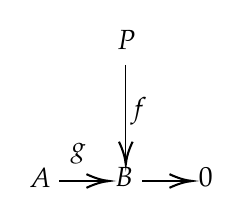
\begin{tikzpicture}[x=0.75pt,y=0.75pt,yscale=-1,xscale=1]
%uncomment if require: \path (0,476); %set diagram left start at 0, and has height of 476

%Straight Lines [id:da9756784236125315] 
\draw    (288,160) -- (288,206) ;
\draw [shift={(288,208)}, rotate = 270] [color={rgb, 255:red, 0; green, 0; blue, 0 }  ][line width=0.75]    (10.93,-3.29) .. controls (6.95,-1.4) and (3.31,-0.3) .. (0,0) .. controls (3.31,0.3) and (6.95,1.4) .. (10.93,3.29)   ;
%Straight Lines [id:da3791632771502693] 
\draw    (256,216) -- (278,216) ;
\draw [shift={(280,216)}, rotate = 180] [color={rgb, 255:red, 0; green, 0; blue, 0 }  ][line width=0.75]    (10.93,-3.29) .. controls (6.95,-1.4) and (3.31,-0.3) .. (0,0) .. controls (3.31,0.3) and (6.95,1.4) .. (10.93,3.29)   ;
%Straight Lines [id:da48034704105691794] 
\draw    (296,216) -- (318,216) ;
\draw [shift={(320,216)}, rotate = 180] [color={rgb, 255:red, 0; green, 0; blue, 0 }  ][line width=0.75]    (10.93,-3.29) .. controls (6.95,-1.4) and (3.31,-0.3) .. (0,0) .. controls (3.31,0.3) and (6.95,1.4) .. (10.93,3.29)   ;

% Text Node
\draw (283,142.4) node [anchor=north west][inner sep=0.75pt]    {$P$};
% Text Node
\draw (241,208.4) node [anchor=north west][inner sep=0.75pt]    {$A$};
% Text Node
\draw (282,208.4) node [anchor=north west][inner sep=0.75pt]    {$B$};
% Text Node
\draw (322,208.4) node [anchor=north west][inner sep=0.75pt]    {$0$};
% Text Node
\draw (289,174.4) node [anchor=north west][inner sep=0.75pt]    {$f$};
% Text Node
\draw (260,196.4) node [anchor=north west][inner sep=0.75pt]    {$g$};


\end{tikzpicture}
\end{center}
with the bottom row exact, i.e. $g$ is an epimorphism, there exists an $R$-module homomorphism $h:P\to A$ such that the diagram 
\begin{center}


\tikzset{every picture/.style={line width=0.75pt}} %set default line width to 0.75pt        

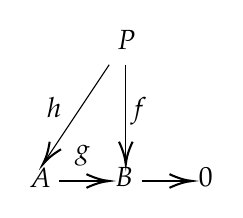
\begin{tikzpicture}[x=0.75pt,y=0.75pt,yscale=-1,xscale=1]
%uncomment if require: \path (0,476); %set diagram left start at 0, and has height of 476

%Straight Lines [id:da9756784236125315] 
\draw    (288,160) -- (288,206) ;
\draw [shift={(288,208)}, rotate = 270] [color={rgb, 255:red, 0; green, 0; blue, 0 }  ][line width=0.75]    (10.93,-3.29) .. controls (6.95,-1.4) and (3.31,-0.3) .. (0,0) .. controls (3.31,0.3) and (6.95,1.4) .. (10.93,3.29)   ;
%Straight Lines [id:da3791632771502693] 
\draw    (256,216) -- (278,216) ;
\draw [shift={(280,216)}, rotate = 180] [color={rgb, 255:red, 0; green, 0; blue, 0 }  ][line width=0.75]    (10.93,-3.29) .. controls (6.95,-1.4) and (3.31,-0.3) .. (0,0) .. controls (3.31,0.3) and (6.95,1.4) .. (10.93,3.29)   ;
%Straight Lines [id:da48034704105691794] 
\draw    (296,216) -- (318,216) ;
\draw [shift={(320,216)}, rotate = 180] [color={rgb, 255:red, 0; green, 0; blue, 0 }  ][line width=0.75]    (10.93,-3.29) .. controls (6.95,-1.4) and (3.31,-0.3) .. (0,0) .. controls (3.31,0.3) and (6.95,1.4) .. (10.93,3.29)   ;
%Straight Lines [id:da36787478006497043] 
\draw    (280,160) -- (249.11,206.34) ;
\draw [shift={(248,208)}, rotate = 303.69] [color={rgb, 255:red, 0; green, 0; blue, 0 }  ][line width=0.75]    (10.93,-3.29) .. controls (6.95,-1.4) and (3.31,-0.3) .. (0,0) .. controls (3.31,0.3) and (6.95,1.4) .. (10.93,3.29)   ;

% Text Node
\draw (283,142.4) node [anchor=north west][inner sep=0.75pt]    {$P$};
% Text Node
\draw (241,208.4) node [anchor=north west][inner sep=0.75pt]    {$A$};
% Text Node
\draw (282,208.4) node [anchor=north west][inner sep=0.75pt]    {$B$};
% Text Node
\draw (322,208.4) node [anchor=north west][inner sep=0.75pt]    {$0$};
% Text Node
\draw (289,174.4) node [anchor=north west][inner sep=0.75pt]    {$f$};
% Text Node
\draw (262,197.4) node [anchor=north west][inner sep=0.75pt]    {$g$};
% Text Node
\draw (249,174.4) node [anchor=north west][inner sep=0.75pt]    {$h$};


\end{tikzpicture}
\end{center}
is commutative, i.e. $gh=f$.
\end{definition}
Our first theorem gives many examples of projective modules. 
\begin{theorem}
Every free module $F$ over a ring $R$ with identity is a projective module.
\end{theorem}
\begin{proof}
We may first assume that modules $A$ and $B$ are unitary. Otherwise by Exercise 5.15 we may decompose $A=A_1\oplus A_2$ and $B=B_1\oplus B_2$, where $A_1$ and $B_1$ are unitary and $RA_2=RB_2=0$. Note that $f(P)\subset B_1$ and $g\mid_{A_1}$ is an epimorphism, whence we may consider the following diagram instead: 
\begin{center}


\tikzset{every picture/.style={line width=0.75pt}} %set default line width to 0.75pt        

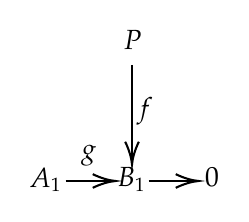
\begin{tikzpicture}[x=0.75pt,y=0.75pt,yscale=-1,xscale=1]
%uncomment if require: \path (0,476); %set diagram left start at 0, and has height of 476

%Straight Lines [id:da9756784236125315] 
\draw    (288,160) -- (288,206) ;
\draw [shift={(288,208)}, rotate = 270] [color={rgb, 255:red, 0; green, 0; blue, 0 }  ][line width=0.75]    (10.93,-3.29) .. controls (6.95,-1.4) and (3.31,-0.3) .. (0,0) .. controls (3.31,0.3) and (6.95,1.4) .. (10.93,3.29)   ;
%Straight Lines [id:da3791632771502693] 
\draw    (256,216) -- (278,216) ;
\draw [shift={(280,216)}, rotate = 180] [color={rgb, 255:red, 0; green, 0; blue, 0 }  ][line width=0.75]    (10.93,-3.29) .. controls (6.95,-1.4) and (3.31,-0.3) .. (0,0) .. controls (3.31,0.3) and (6.95,1.4) .. (10.93,3.29)   ;
%Straight Lines [id:da48034704105691794] 
\draw    (296,216) -- (318,216) ;
\draw [shift={(320,216)}, rotate = 180] [color={rgb, 255:red, 0; green, 0; blue, 0 }  ][line width=0.75]    (10.93,-3.29) .. controls (6.95,-1.4) and (3.31,-0.3) .. (0,0) .. controls (3.31,0.3) and (6.95,1.4) .. (10.93,3.29)   ;

% Text Node
\draw (283,142.4) node [anchor=north west][inner sep=0.75pt]    {$P$};
% Text Node
\draw (238,208.4) node [anchor=north west][inner sep=0.75pt]    {$A_{1}$};
% Text Node
\draw (280,208.4) node [anchor=north west][inner sep=0.75pt]    {$B_{1}$};
% Text Node
\draw (322,208.4) node [anchor=north west][inner sep=0.75pt]    {$0$};
% Text Node
\draw (289,174.4) node [anchor=north west][inner sep=0.75pt]    {$f$};
% Text Node
\draw (262,197.4) node [anchor=north west][inner sep=0.75pt]    {$g$};


\end{tikzpicture}
\end{center}
Now suppose $F$ is a free $R$-module and $A$ and $B$ are unitary. Therefore $F$ is spanned by a basis $X$. Suppose $\iota:X\to F$ is the canonical injection. Since $g$ is an epimorphism, there exists some $a_x\in A$ such that $g(a_x)=f(\iota(x))$. Define $h:x\mapsto a_x$. Since $h$ is determined by elements of $X$, we finished our proof.
\end{proof}
\begin{corollary}
Every module $A$ over a ring $R$ is the homomorphic image of a projective $R$-module.
\end{corollary}
\begin{proof}
By Corollary 5.14 we know that every module $A$ over a ring $R$ is the homomorphic image of a free module. Apply Theorem 5.27 we know that every free module over a ring $R$ is projective, and the proof is finished.
\end{proof}
\begin{theorem}
Let $R$ be a ring. The following conditions on an $R$-module $P$ are equivalent.\par
(a) $P$ is projective;\par
(b) every short exact sequence $0\longrightarrow A\overset{f}{\longrightarrow}B\overset{g}{\longrightarrow}P\longrightarrow 0$ is split exact;\par
(c) there is a free module $F$ and an $R$-module $K$ such that $F\cong K\oplus P$.
\end{theorem}
\begin{proof}
(a)$\Rightarrow$(b): Consider the following diagram: 
\begin{center}


\tikzset{every picture/.style={line width=0.75pt}} %set default line width to 0.75pt        

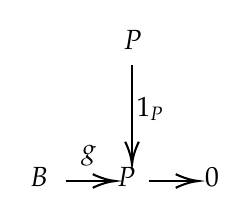
\begin{tikzpicture}[x=0.75pt,y=0.75pt,yscale=-1,xscale=1]
%uncomment if require: \path (0,476); %set diagram left start at 0, and has height of 476

%Straight Lines [id:da9756784236125315] 
\draw    (288,160) -- (288,206) ;
\draw [shift={(288,208)}, rotate = 270] [color={rgb, 255:red, 0; green, 0; blue, 0 }  ][line width=0.75]    (10.93,-3.29) .. controls (6.95,-1.4) and (3.31,-0.3) .. (0,0) .. controls (3.31,0.3) and (6.95,1.4) .. (10.93,3.29)   ;
%Straight Lines [id:da3791632771502693] 
\draw    (256,216) -- (278,216) ;
\draw [shift={(280,216)}, rotate = 180] [color={rgb, 255:red, 0; green, 0; blue, 0 }  ][line width=0.75]    (10.93,-3.29) .. controls (6.95,-1.4) and (3.31,-0.3) .. (0,0) .. controls (3.31,0.3) and (6.95,1.4) .. (10.93,3.29)   ;
%Straight Lines [id:da48034704105691794] 
\draw    (296,216) -- (318,216) ;
\draw [shift={(320,216)}, rotate = 180] [color={rgb, 255:red, 0; green, 0; blue, 0 }  ][line width=0.75]    (10.93,-3.29) .. controls (6.95,-1.4) and (3.31,-0.3) .. (0,0) .. controls (3.31,0.3) and (6.95,1.4) .. (10.93,3.29)   ;

% Text Node
\draw (283,142.4) node [anchor=north west][inner sep=0.75pt]    {$P$};
% Text Node
\draw (238,208.4) node [anchor=north west][inner sep=0.75pt]    {$B$};
% Text Node
\draw (280,208.4) node [anchor=north west][inner sep=0.75pt]    {$P$};
% Text Node
\draw (322,208.4) node [anchor=north west][inner sep=0.75pt]    {$0$};
% Text Node
\draw (289,174.4) node [anchor=north west][inner sep=0.75pt]    {$1_{P}$};
% Text Node
\draw (262,197.4) node [anchor=north west][inner sep=0.75pt]    {$g$};


\end{tikzpicture}
\end{center}
Since $P$ is projective, there exists an $R$-module homomorphism $h:P\to B$ such that $hg=1_P$. Therefore the short exact sequence 
$$0\longrightarrow A\overset{f}{\longrightarrow}B\overset{g}{\longrightarrow}P\longrightarrow 0$$
split, and $B\cong A\oplus P$.\par
(b)$\Rightarrow$(c): Since $F$ is a free module, there exists an epimorphism $g:F\to P$. Let $K=\mathrm{Ker}g$, then we have the short exact sequence 
$$
0\longrightarrow K\longrightarrow F\overset{g}{\longrightarrow}P\longrightarrow 0
$$
is split exact. Therefore $F\cong K\oplus P$.\par
(c)$\Rightarrow$(a): By condition we know that the short exact sequence 
$$
0\longrightarrow K\longrightarrow F\longrightarrow P\longrightarrow 0
$$
split, therefore there exists some $h:P\to F$ such that $hg=1$, here $g:F\to P$ be the canonical injection. Therefore we proved that $P$ is projective.
\end{proof}
We give some examples that are projective modules but not free modules. Consider $\mathbb{Z}_2$ and $\mathbb{Z}_3$. Since $\mathbb{Z}_2$ and $\mathbb{Z}_3$ are $\mathbb{Z}_6$ modules and $\mathbb{Z}_6\cong\mathbb{Z}_2\oplus\mathbb{Z}_3$, we have the short exact sequence 
$$
0\longrightarrow \mathbb{Z} _2\longrightarrow \mathbb{Z} _2\oplus \mathbb{Z} _3\longrightarrow \mathbb{Z} _3\longrightarrow 0
$$
split, and hence by Theorem 5.29 we know that $\mathbb{Z}_2$ and $\mathbb{Z}_3$ are projective but not free $\mathbb{Z}_6$-modules.
\begin{proposition}
Let $R$ be a ring. A direct sum of $R$-modules $\bigoplus_{i\in I}P_i$ is projective if and only if each $P_i$ is projective.
\end{proposition}
\begin{proof}
Suppose $\bigoplus_{i\in I}P_i$ is projective. Then for each $P_j$, we have the following diagram: 
\begin{center}


\tikzset{every picture/.style={line width=0.75pt}} %set default line width to 0.75pt        

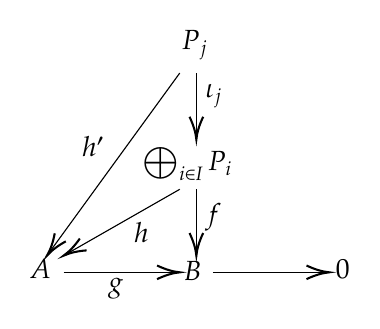
\begin{tikzpicture}[x=0.75pt,y=0.75pt,yscale=-1,xscale=1]
%uncomment if require: \path (0,476); %set diagram left start at 0, and has height of 476

%Straight Lines [id:da4410470739213719] 
\draw    (304,96) -- (304,126) ;
\draw [shift={(304,128)}, rotate = 270] [color={rgb, 255:red, 0; green, 0; blue, 0 }  ][line width=0.75]    (10.93,-3.29) .. controls (6.95,-1.4) and (3.31,-0.3) .. (0,0) .. controls (3.31,0.3) and (6.95,1.4) .. (10.93,3.29)   ;
%Straight Lines [id:da11715093568326385] 
\draw    (304,152) -- (304,182) ;
\draw [shift={(304,184)}, rotate = 270] [color={rgb, 255:red, 0; green, 0; blue, 0 }  ][line width=0.75]    (10.93,-3.29) .. controls (6.95,-1.4) and (3.31,-0.3) .. (0,0) .. controls (3.31,0.3) and (6.95,1.4) .. (10.93,3.29)   ;
%Straight Lines [id:da11098979119714536] 
\draw    (312,192) -- (366,192) ;
\draw [shift={(368,192)}, rotate = 180] [color={rgb, 255:red, 0; green, 0; blue, 0 }  ][line width=0.75]    (10.93,-3.29) .. controls (6.95,-1.4) and (3.31,-0.3) .. (0,0) .. controls (3.31,0.3) and (6.95,1.4) .. (10.93,3.29)   ;
%Straight Lines [id:da38705239794661384] 
\draw    (240,192) -- (294,192) ;
\draw [shift={(296,192)}, rotate = 180] [color={rgb, 255:red, 0; green, 0; blue, 0 }  ][line width=0.75]    (10.93,-3.29) .. controls (6.95,-1.4) and (3.31,-0.3) .. (0,0) .. controls (3.31,0.3) and (6.95,1.4) .. (10.93,3.29)   ;
%Straight Lines [id:da7846735142684917] 
\draw    (296,152) -- (241.74,183.01) ;
\draw [shift={(240,184)}, rotate = 330.26] [color={rgb, 255:red, 0; green, 0; blue, 0 }  ][line width=0.75]    (10.93,-3.29) .. controls (6.95,-1.4) and (3.31,-0.3) .. (0,0) .. controls (3.31,0.3) and (6.95,1.4) .. (10.93,3.29)   ;
%Straight Lines [id:da6462873867895451] 
\draw    (296,96) -- (233.18,182.38) ;
\draw [shift={(232,184)}, rotate = 306.03] [color={rgb, 255:red, 0; green, 0; blue, 0 }  ][line width=0.75]    (10.93,-3.29) .. controls (6.95,-1.4) and (3.31,-0.3) .. (0,0) .. controls (3.31,0.3) and (6.95,1.4) .. (10.93,3.29)   ;

% Text Node
\draw (296,74.4) node [anchor=north west][inner sep=0.75pt]    {$P_{j}$};
% Text Node
\draw (277,130.4) node [anchor=north west][inner sep=0.75pt]    {$\bigoplus _{i\in I} P_{i}$};
% Text Node
\draw (297,185.4) node [anchor=north west][inner sep=0.75pt]    {$B$};
% Text Node
\draw (223,184.4) node [anchor=north west][inner sep=0.75pt]    {$A$};
% Text Node
\draw (370,184.4) node [anchor=north west][inner sep=0.75pt]    {$0$};
% Text Node
\draw (307,157.4) node [anchor=north west][inner sep=0.75pt]    {$f$};
% Text Node
\draw (260,193.4) node [anchor=north west][inner sep=0.75pt]    {$g$};
% Text Node
\draw (273,166.4) node [anchor=north west][inner sep=0.75pt]    {$h$};
% Text Node
\draw (248,125.4) node [anchor=north west][inner sep=0.75pt]    {$h^{\prime }$};
% Text Node
\draw (307,100.4) node [anchor=north west][inner sep=0.75pt]    {$\iota _{j}$};


\end{tikzpicture}
\end{center}
Since $\bigoplus_{i\in I}P_i$ is projective, then there exists some $h$ such that $gh=f$. Now define $h^\prime=h\iota_j$, we have $gh^\prime =gh\iota_j=f\iota_j$, whence $h^\prime$ satisfies the condition and hence $P_j$ is projective. Conversely, we have the following diagram:
\begin{center}


\tikzset{every picture/.style={line width=0.75pt}} %set default line width to 0.75pt        

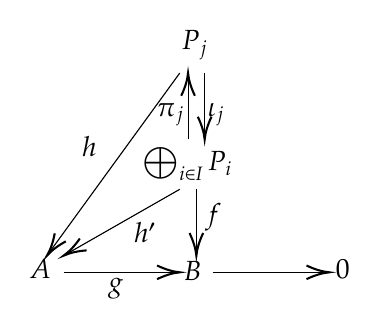
\begin{tikzpicture}[x=0.75pt,y=0.75pt,yscale=-1,xscale=1]
%uncomment if require: \path (0,476); %set diagram left start at 0, and has height of 476

%Straight Lines [id:da4410470739213719] 
\draw    (308,96) -- (308,126) ;
\draw [shift={(308,128)}, rotate = 270] [color={rgb, 255:red, 0; green, 0; blue, 0 }  ][line width=0.75]    (10.93,-3.29) .. controls (6.95,-1.4) and (3.31,-0.3) .. (0,0) .. controls (3.31,0.3) and (6.95,1.4) .. (10.93,3.29)   ;
%Straight Lines [id:da11715093568326385] 
\draw    (304,152) -- (304,182) ;
\draw [shift={(304,184)}, rotate = 270] [color={rgb, 255:red, 0; green, 0; blue, 0 }  ][line width=0.75]    (10.93,-3.29) .. controls (6.95,-1.4) and (3.31,-0.3) .. (0,0) .. controls (3.31,0.3) and (6.95,1.4) .. (10.93,3.29)   ;
%Straight Lines [id:da11098979119714536] 
\draw    (312,192) -- (366,192) ;
\draw [shift={(368,192)}, rotate = 180] [color={rgb, 255:red, 0; green, 0; blue, 0 }  ][line width=0.75]    (10.93,-3.29) .. controls (6.95,-1.4) and (3.31,-0.3) .. (0,0) .. controls (3.31,0.3) and (6.95,1.4) .. (10.93,3.29)   ;
%Straight Lines [id:da38705239794661384] 
\draw    (240,192) -- (294,192) ;
\draw [shift={(296,192)}, rotate = 180] [color={rgb, 255:red, 0; green, 0; blue, 0 }  ][line width=0.75]    (10.93,-3.29) .. controls (6.95,-1.4) and (3.31,-0.3) .. (0,0) .. controls (3.31,0.3) and (6.95,1.4) .. (10.93,3.29)   ;
%Straight Lines [id:da7846735142684917] 
\draw    (296,152) -- (241.74,183.01) ;
\draw [shift={(240,184)}, rotate = 330.26] [color={rgb, 255:red, 0; green, 0; blue, 0 }  ][line width=0.75]    (10.93,-3.29) .. controls (6.95,-1.4) and (3.31,-0.3) .. (0,0) .. controls (3.31,0.3) and (6.95,1.4) .. (10.93,3.29)   ;
%Straight Lines [id:da6462873867895451] 
\draw    (296,96) -- (233.18,182.38) ;
\draw [shift={(232,184)}, rotate = 306.03] [color={rgb, 255:red, 0; green, 0; blue, 0 }  ][line width=0.75]    (10.93,-3.29) .. controls (6.95,-1.4) and (3.31,-0.3) .. (0,0) .. controls (3.31,0.3) and (6.95,1.4) .. (10.93,3.29)   ;
%Straight Lines [id:da7889817906156957] 
\draw    (300,128) -- (300,98) ;
\draw [shift={(300,96)}, rotate = 90] [color={rgb, 255:red, 0; green, 0; blue, 0 }  ][line width=0.75]    (10.93,-3.29) .. controls (6.95,-1.4) and (3.31,-0.3) .. (0,0) .. controls (3.31,0.3) and (6.95,1.4) .. (10.93,3.29)   ;

% Text Node
\draw (296,74.4) node [anchor=north west][inner sep=0.75pt]    {$P_{j}$};
% Text Node
\draw (277,130.4) node [anchor=north west][inner sep=0.75pt]    {$\bigoplus _{i\in I} P_{i}$};
% Text Node
\draw (297,185.4) node [anchor=north west][inner sep=0.75pt]    {$B$};
% Text Node
\draw (223,184.4) node [anchor=north west][inner sep=0.75pt]    {$A$};
% Text Node
\draw (370,184.4) node [anchor=north west][inner sep=0.75pt]    {$0$};
% Text Node
\draw (307,157.4) node [anchor=north west][inner sep=0.75pt]    {$f$};
% Text Node
\draw (260,193.4) node [anchor=north west][inner sep=0.75pt]    {$g$};
% Text Node
\draw (273,166.4) node [anchor=north west][inner sep=0.75pt]    {$h^{\prime }$};
% Text Node
\draw (248,125.4) node [anchor=north west][inner sep=0.75pt]    {$h$};
% Text Node
\draw (308,109.4) node [anchor=north west][inner sep=0.75pt]    {$\iota _{j}$};
% Text Node
\draw (284,109.4) node [anchor=north west][inner sep=0.75pt]    {$\pi _{j}$};


\end{tikzpicture}
\end{center}
Define $h^\prime=\sum_{j\in I}h\pi_j$, then we have 
$$
gh=g\left( \sum_{j\in I}{h\pi _j} \right) =\sum_{j\in I}{gh\pi _j}=\sum_{j\in I}{f\iota _j\pi _j}=f,
$$
which finished the proof.
\end{proof}
Recall that the dual of a concept in category is defined by reversing all arrows. Pushing this idea a bit further one might say that the dual of a monomorphism is epimorphism, since $A\to B$ is monomorphism if and only if $0\longrightarrow A\longrightarrow B$ is exact, and if $A\to B$ is an epimorphism if and only if $B\longrightarrow A\longrightarrow 0$ is exact, which arrows reversed. This leads us to the definition of the dual notion of projective modules in the following way.
\begin{definition}
A module $J$ over a ring $R$ is said to be \textbf{injective} if given any diagram of $R$-module homomorphisms 
\begin{center}


\tikzset{every picture/.style={line width=0.75pt}} %set default line width to 0.75pt        

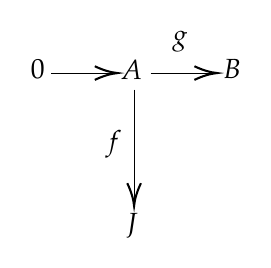
\begin{tikzpicture}[x=0.75pt,y=0.75pt,yscale=-1,xscale=1]
%uncomment if require: \path (0,476); %set diagram left start at 0, and has height of 476

%Straight Lines [id:da2979778987226902] 
\draw    (232,120) -- (262,120) ;
\draw [shift={(264,120)}, rotate = 180] [color={rgb, 255:red, 0; green, 0; blue, 0 }  ][line width=0.75]    (10.93,-3.29) .. controls (6.95,-1.4) and (3.31,-0.3) .. (0,0) .. controls (3.31,0.3) and (6.95,1.4) .. (10.93,3.29)   ;
%Straight Lines [id:da1283630480544964] 
\draw    (280,120) -- (310,120) ;
\draw [shift={(312,120)}, rotate = 180] [color={rgb, 255:red, 0; green, 0; blue, 0 }  ][line width=0.75]    (10.93,-3.29) .. controls (6.95,-1.4) and (3.31,-0.3) .. (0,0) .. controls (3.31,0.3) and (6.95,1.4) .. (10.93,3.29)   ;
%Straight Lines [id:da5874779160595505] 
\draw    (272,128) -- (272,182) ;
\draw [shift={(272,184)}, rotate = 270] [color={rgb, 255:red, 0; green, 0; blue, 0 }  ][line width=0.75]    (10.93,-3.29) .. controls (6.95,-1.4) and (3.31,-0.3) .. (0,0) .. controls (3.31,0.3) and (6.95,1.4) .. (10.93,3.29)   ;

% Text Node
\draw (221,112.4) node [anchor=north west][inner sep=0.75pt]    {$0$};
% Text Node
\draw (265,112.4) node [anchor=north west][inner sep=0.75pt]    {$A$};
% Text Node
\draw (314,112.4) node [anchor=north west][inner sep=0.75pt]    {$B$};
% Text Node
\draw (267,186.4) node [anchor=north west][inner sep=0.75pt]    {$J$};
% Text Node
\draw (289,98.4) node [anchor=north west][inner sep=0.75pt]    {$g$};
% Text Node
\draw (257,146.4) node [anchor=north west][inner sep=0.75pt]    {$f$};


\end{tikzpicture}
\end{center}
with top row exact, i.e., $g$ is an epimorphism, there exists an $R$-module homomorphism $h:B\to J$ such that the diagram 
\begin{center}


\tikzset{every picture/.style={line width=0.75pt}} %set default line width to 0.75pt        

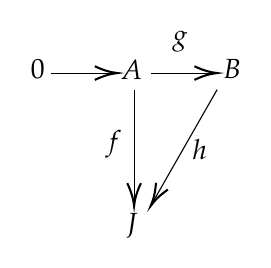
\begin{tikzpicture}[x=0.75pt,y=0.75pt,yscale=-1,xscale=1]
%uncomment if require: \path (0,476); %set diagram left start at 0, and has height of 476

%Straight Lines [id:da2979778987226902] 
\draw    (232,120) -- (262,120) ;
\draw [shift={(264,120)}, rotate = 180] [color={rgb, 255:red, 0; green, 0; blue, 0 }  ][line width=0.75]    (10.93,-3.29) .. controls (6.95,-1.4) and (3.31,-0.3) .. (0,0) .. controls (3.31,0.3) and (6.95,1.4) .. (10.93,3.29)   ;
%Straight Lines [id:da1283630480544964] 
\draw    (280,120) -- (310,120) ;
\draw [shift={(312,120)}, rotate = 180] [color={rgb, 255:red, 0; green, 0; blue, 0 }  ][line width=0.75]    (10.93,-3.29) .. controls (6.95,-1.4) and (3.31,-0.3) .. (0,0) .. controls (3.31,0.3) and (6.95,1.4) .. (10.93,3.29)   ;
%Straight Lines [id:da5874779160595505] 
\draw    (272,128) -- (272,182) ;
\draw [shift={(272,184)}, rotate = 270] [color={rgb, 255:red, 0; green, 0; blue, 0 }  ][line width=0.75]    (10.93,-3.29) .. controls (6.95,-1.4) and (3.31,-0.3) .. (0,0) .. controls (3.31,0.3) and (6.95,1.4) .. (10.93,3.29)   ;
%Straight Lines [id:da03644286916885808] 
\draw    (312,128) -- (280.99,182.26) ;
\draw [shift={(280,184)}, rotate = 299.74] [color={rgb, 255:red, 0; green, 0; blue, 0 }  ][line width=0.75]    (10.93,-3.29) .. controls (6.95,-1.4) and (3.31,-0.3) .. (0,0) .. controls (3.31,0.3) and (6.95,1.4) .. (10.93,3.29)   ;

% Text Node
\draw (221,112.4) node [anchor=north west][inner sep=0.75pt]    {$0$};
% Text Node
\draw (265,112.4) node [anchor=north west][inner sep=0.75pt]    {$A$};
% Text Node
\draw (314,112.4) node [anchor=north west][inner sep=0.75pt]    {$B$};
% Text Node
\draw (267,186.4) node [anchor=north west][inner sep=0.75pt]    {$J$};
% Text Node
\draw (289,98.4) node [anchor=north west][inner sep=0.75pt]    {$g$};
% Text Node
\draw (257,146.4) node [anchor=north west][inner sep=0.75pt]    {$f$};
% Text Node
\draw (299,150.4) node [anchor=north west][inner sep=0.75pt]    {$h$};


\end{tikzpicture}
\end{center}
is commutative, i.e. $hg=f$.
\end{definition}
It is not surprising that many of the preceding propositions about projective modules are readily proved. For example, since the dual of direct sums (coproducts) are products, the dual of Proposition 5.30 is the following:
\begin{proposition}
A direct product of $R$-modules $\prod_{i\in I}J_i$ is injective if and only if each $J_i$ is injective.
\end{proposition}
\begin{proof}
By duality and proposition 5.30, we finished the proof.
\end{proof}
Since the concept of free module can not be dualized, there are no analogues of Theorem 5.27 or Theorem 5.29(iii) for injective modules. However, Corollary 5.28 can be dualized. It states, in effect, that for every module $A$ there is a projective module $P$ and an exact sequence $P\longrightarrow A\longrightarrow 0$. The dual of this statement is that for every module $A$ there is an injective module $J$ and an exact sequence $0\longrightarrow A\longrightarrow J$; in other words, every module may be embedded in an injective module. The remainder of this section is devoted to proving this fact for unitary modules over a ring with identity.
\begin{lemma}\em
Let $R$ be a ring with identity. A unitary $R$-module $J$ is injective if and only if for every left ideal $L$ of $R$, any $R$-module homomorphism $L\to J$ may be extended to an $R$-module homomorphism $R\to J$.
\end{lemma}
\begin{proof}
Suppose $J$ is injective, then we have the following commutative diagram: 
\begin{center}


\tikzset{every picture/.style={line width=0.75pt}} %set default line width to 0.75pt        

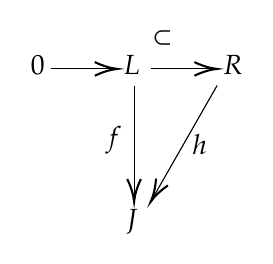
\begin{tikzpicture}[x=0.75pt,y=0.75pt,yscale=-1,xscale=1]
%uncomment if require: \path (0,476); %set diagram left start at 0, and has height of 476

%Straight Lines [id:da2979778987226902] 
\draw    (232,120) -- (262,120) ;
\draw [shift={(264,120)}, rotate = 180] [color={rgb, 255:red, 0; green, 0; blue, 0 }  ][line width=0.75]    (10.93,-3.29) .. controls (6.95,-1.4) and (3.31,-0.3) .. (0,0) .. controls (3.31,0.3) and (6.95,1.4) .. (10.93,3.29)   ;
%Straight Lines [id:da1283630480544964] 
\draw    (280,120) -- (310,120) ;
\draw [shift={(312,120)}, rotate = 180] [color={rgb, 255:red, 0; green, 0; blue, 0 }  ][line width=0.75]    (10.93,-3.29) .. controls (6.95,-1.4) and (3.31,-0.3) .. (0,0) .. controls (3.31,0.3) and (6.95,1.4) .. (10.93,3.29)   ;
%Straight Lines [id:da5874779160595505] 
\draw    (272,128) -- (272,182) ;
\draw [shift={(272,184)}, rotate = 270] [color={rgb, 255:red, 0; green, 0; blue, 0 }  ][line width=0.75]    (10.93,-3.29) .. controls (6.95,-1.4) and (3.31,-0.3) .. (0,0) .. controls (3.31,0.3) and (6.95,1.4) .. (10.93,3.29)   ;
%Straight Lines [id:da03644286916885808] 
\draw    (312,128) -- (280.99,182.26) ;
\draw [shift={(280,184)}, rotate = 299.74] [color={rgb, 255:red, 0; green, 0; blue, 0 }  ][line width=0.75]    (10.93,-3.29) .. controls (6.95,-1.4) and (3.31,-0.3) .. (0,0) .. controls (3.31,0.3) and (6.95,1.4) .. (10.93,3.29)   ;

% Text Node
\draw (221,112.4) node [anchor=north west][inner sep=0.75pt]    {$0$};
% Text Node
\draw (266,112.4) node [anchor=north west][inner sep=0.75pt]    {$L$};
% Text Node
\draw (314,112.4) node [anchor=north west][inner sep=0.75pt]    {$R$};
% Text Node
\draw (267,186.4) node [anchor=north west][inner sep=0.75pt]    {$J$};
% Text Node
\draw (280,100.4) node [anchor=north west][inner sep=0.75pt]    {$\subset $};
% Text Node
\draw (257,146.4) node [anchor=north west][inner sep=0.75pt]    {$f$};
% Text Node
\draw (299,150.4) node [anchor=north west][inner sep=0.75pt]    {$h$};


\end{tikzpicture}
\end{center}
whence there exists some $h:R\to J$ be the extension of $f$. Conversely, suppose $J$ has the properties above, we show that $J$ is injective. Suppose we are given the following diagram 
\begin{center}


\tikzset{every picture/.style={line width=0.75pt}} %set default line width to 0.75pt        

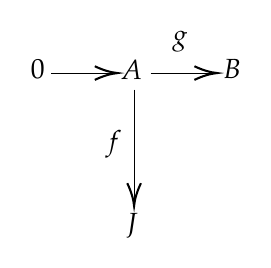
\begin{tikzpicture}[x=0.75pt,y=0.75pt,yscale=-1,xscale=1]
%uncomment if require: \path (0,476); %set diagram left start at 0, and has height of 476

%Straight Lines [id:da2979778987226902] 
\draw    (232,120) -- (262,120) ;
\draw [shift={(264,120)}, rotate = 180] [color={rgb, 255:red, 0; green, 0; blue, 0 }  ][line width=0.75]    (10.93,-3.29) .. controls (6.95,-1.4) and (3.31,-0.3) .. (0,0) .. controls (3.31,0.3) and (6.95,1.4) .. (10.93,3.29)   ;
%Straight Lines [id:da1283630480544964] 
\draw    (280,120) -- (310,120) ;
\draw [shift={(312,120)}, rotate = 180] [color={rgb, 255:red, 0; green, 0; blue, 0 }  ][line width=0.75]    (10.93,-3.29) .. controls (6.95,-1.4) and (3.31,-0.3) .. (0,0) .. controls (3.31,0.3) and (6.95,1.4) .. (10.93,3.29)   ;
%Straight Lines [id:da5874779160595505] 
\draw    (272,128) -- (272,182) ;
\draw [shift={(272,184)}, rotate = 270] [color={rgb, 255:red, 0; green, 0; blue, 0 }  ][line width=0.75]    (10.93,-3.29) .. controls (6.95,-1.4) and (3.31,-0.3) .. (0,0) .. controls (3.31,0.3) and (6.95,1.4) .. (10.93,3.29)   ;

% Text Node
\draw (221,112.4) node [anchor=north west][inner sep=0.75pt]    {$0$};
% Text Node
\draw (265,112.4) node [anchor=north west][inner sep=0.75pt]    {$A$};
% Text Node
\draw (314,112.4) node [anchor=north west][inner sep=0.75pt]    {$B$};
% Text Node
\draw (267,186.4) node [anchor=north west][inner sep=0.75pt]    {$J$};
% Text Node
\draw (289,98.4) node [anchor=north west][inner sep=0.75pt]    {$g$};
% Text Node
\draw (257,146.4) node [anchor=north west][inner sep=0.75pt]    {$f$};


\end{tikzpicture}
\end{center}
with the top row exact. Then we define a collection of $R$-module homomorphisms $\mathcal{S}$, whose elements are homomorphisms $h:C\to J$, where $\mathrm{Im}g\subset C\subset B$. Clearly $\mathcal{S}$ is nonempty, since $fg^{-1}\in\mathcal{S}$. We define the order on $\mathcal{S}$ as follows: We say $h_1\prec h_2$, if $\mathrm{Dom}h_1\subset\mathrm{Dom}h_2$ and $h_2\mid_{\mathrm{Dom}h_1}=h_1$. Then by Zorn's Lemma there exists some maximal element $h:H\to J$. Now it suffices to show that $H=B$.\par
Suppose not, let $b\in B-H$. Then $L=\{r\in R:rb\in H\}$ is a left ideal of $R$. The map $L\to J$ given by $r\mapsto h(rb)$ is a well-defined homomorphism. Therefore by our hypothesis there exists an $R$-module homomorphism $k:R\to J$ such that $k(r)=h(rb)$ for all $r\in R$, as the following diagram shows.
\begin{center}


\tikzset{every picture/.style={line width=0.75pt}} %set default line width to 0.75pt        

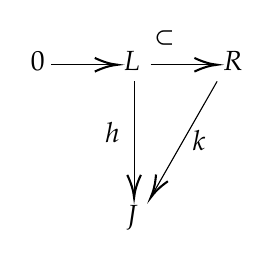
\begin{tikzpicture}[x=0.75pt,y=0.75pt,yscale=-1,xscale=1]
%uncomment if require: \path (0,476); %set diagram left start at 0, and has height of 476

%Straight Lines [id:da2979778987226902] 
\draw    (232,120) -- (262,120) ;
\draw [shift={(264,120)}, rotate = 180] [color={rgb, 255:red, 0; green, 0; blue, 0 }  ][line width=0.75]    (10.93,-3.29) .. controls (6.95,-1.4) and (3.31,-0.3) .. (0,0) .. controls (3.31,0.3) and (6.95,1.4) .. (10.93,3.29)   ;
%Straight Lines [id:da1283630480544964] 
\draw    (280,120) -- (310,120) ;
\draw [shift={(312,120)}, rotate = 180] [color={rgb, 255:red, 0; green, 0; blue, 0 }  ][line width=0.75]    (10.93,-3.29) .. controls (6.95,-1.4) and (3.31,-0.3) .. (0,0) .. controls (3.31,0.3) and (6.95,1.4) .. (10.93,3.29)   ;
%Straight Lines [id:da5874779160595505] 
\draw    (272,128) -- (272,182) ;
\draw [shift={(272,184)}, rotate = 270] [color={rgb, 255:red, 0; green, 0; blue, 0 }  ][line width=0.75]    (10.93,-3.29) .. controls (6.95,-1.4) and (3.31,-0.3) .. (0,0) .. controls (3.31,0.3) and (6.95,1.4) .. (10.93,3.29)   ;
%Straight Lines [id:da4095127738212234] 
\draw    (312,128) -- (280.99,182.26) ;
\draw [shift={(280,184)}, rotate = 299.74] [color={rgb, 255:red, 0; green, 0; blue, 0 }  ][line width=0.75]    (10.93,-3.29) .. controls (6.95,-1.4) and (3.31,-0.3) .. (0,0) .. controls (3.31,0.3) and (6.95,1.4) .. (10.93,3.29)   ;

% Text Node
\draw (221,112.4) node [anchor=north west][inner sep=0.75pt]    {$0$};
% Text Node
\draw (266,112.4) node [anchor=north west][inner sep=0.75pt]    {$L$};
% Text Node
\draw (314,112.4) node [anchor=north west][inner sep=0.75pt]    {$R$};
% Text Node
\draw (267,186.4) node [anchor=north west][inner sep=0.75pt]    {$J$};
% Text Node
\draw (281,102.4) node [anchor=north west][inner sep=0.75pt]    {$\subset $};
% Text Node
\draw (257,146.4) node [anchor=north west][inner sep=0.75pt]    {$h$};
% Text Node
\draw (299,150.4) node [anchor=north west][inner sep=0.75pt]    {$k$};


\end{tikzpicture}
\end{center}
Let $c=k(1_R)$ and define a map $\overline{h}:H+Rb\to J$ given by $a+rb\mapsto h(a)+rc$. Then it is easy to verify that $\overline{h}$ is well-defined and an $R$-module homomorphism. However, $h\prec\overline{h}$, which contradict to the fact that $h$ is a maximal element. Therefore $H=B$, and the proof is finished.
\end{proof}
An abelian group $D$ is said to be \textbf{divisible}, if given any $y\in D$ and $0\ne n\in\mathbb{Z}$, there exists $x\in D$ such that $nx=y$. For example, the additive group $\mathbb{Q}$ is divisible. However $\mathbb{Z}$ is not. The next lemma gives a characterization of divisible groups.
\begin{lemma}\em
An abelian group $D$ is divisible if and only if $D$ is an injective (unitary) $\mathbb{Z}$-module.
\end{lemma}
\begin{proof}
Suppose $D$ is divisible. Then let $y\in D$ and $0\ne n\in\mathbb{Z}$, we consider the homomorphism $f:\left<n\right>\to D$ determined by $n\mapsto y$. Since $D$ is injective, there is a homomorphism $h:\mathbb{Z}\to D$ such that the diagram 
\begin{center}


\tikzset{every picture/.style={line width=0.75pt}} %set default line width to 0.75pt        

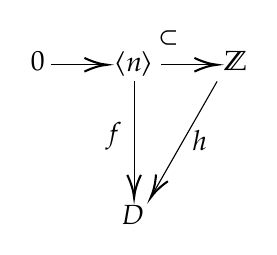
\begin{tikzpicture}[x=0.75pt,y=0.75pt,yscale=-1,xscale=1]
%uncomment if require: \path (0,476); %set diagram left start at 0, and has height of 476

%Straight Lines [id:da2979778987226902] 
\draw    (232,120) -- (257,120) ;
\draw [shift={(259,120)}, rotate = 180] [color={rgb, 255:red, 0; green, 0; blue, 0 }  ][line width=0.75]    (10.93,-3.29) .. controls (6.95,-1.4) and (3.31,-0.3) .. (0,0) .. controls (3.31,0.3) and (6.95,1.4) .. (10.93,3.29)   ;
%Straight Lines [id:da1283630480544964] 
\draw    (285,120) -- (310,120) ;
\draw [shift={(312,120)}, rotate = 180] [color={rgb, 255:red, 0; green, 0; blue, 0 }  ][line width=0.75]    (10.93,-3.29) .. controls (6.95,-1.4) and (3.31,-0.3) .. (0,0) .. controls (3.31,0.3) and (6.95,1.4) .. (10.93,3.29)   ;
%Straight Lines [id:da5874779160595505] 
\draw    (272,128) -- (272,182) ;
\draw [shift={(272,184)}, rotate = 270] [color={rgb, 255:red, 0; green, 0; blue, 0 }  ][line width=0.75]    (10.93,-3.29) .. controls (6.95,-1.4) and (3.31,-0.3) .. (0,0) .. controls (3.31,0.3) and (6.95,1.4) .. (10.93,3.29)   ;
%Straight Lines [id:da4095127738212234] 
\draw    (312,128) -- (280.99,182.26) ;
\draw [shift={(280,184)}, rotate = 299.74] [color={rgb, 255:red, 0; green, 0; blue, 0 }  ][line width=0.75]    (10.93,-3.29) .. controls (6.95,-1.4) and (3.31,-0.3) .. (0,0) .. controls (3.31,0.3) and (6.95,1.4) .. (10.93,3.29)   ;

% Text Node
\draw (221,112.4) node [anchor=north west][inner sep=0.75pt]    {$0$};
% Text Node
\draw (262,112.4) node [anchor=north west][inner sep=0.75pt]    {$\left<n\right>$};
% Text Node
\draw (314,112.4) node [anchor=north west][inner sep=0.75pt]    {$\mathbb{Z}$};
% Text Node
\draw (265,186.4) node [anchor=north west][inner sep=0.75pt]    {$D$};
% Text Node
\draw (283,102.4) node [anchor=north west][inner sep=0.75pt]    {$\subset $};
% Text Node
\draw (257,146.4) node [anchor=north west][inner sep=0.75pt]    {$f$};
% Text Node
\draw (299,150.4) node [anchor=north west][inner sep=0.75pt]    {$h$};


\end{tikzpicture}
\end{center}
is commutative. Let $h(1)=x$, then $nx=nh(1)=h(n)=y$, whence $D$ is divisible. Conversely, suppose $D$ is divisible, then since the ideal of $\mathbb{Z}$ are of the form $\left<n\right>$, then there exists some $x\in D$ such that $nx=f(n)$, where $f:\left<n\right>$ is the homomorphism defined by $n\mapsto a_x$. Define $h:\mathbb{Z}\to D$ by $1\mapsto x$, therefore $h$ is the extension of $f$, whence $D$ is injective by Lemma 5.4.
\end{proof}
\begin{lemma}\em
Every abelian group $A$ may be embedded in a divisible abelian group.
\end{lemma}
\begin{proof}
Since $A$ is an abelian group, we know that $A$ is a $\mathbb{Z}$-module, and hence a homomorphic image of some free $\mathbb{Z}$-module $F$. Therefore $A\cong F/K$. Note that $F\cong\bigoplus\mathbb{Z}$, and each $\mathbb{Z}$ can be embedded into the divisible group $\mathbb{Q}$, therefore 
$$
A\cong F/K\cong \left( \bigoplus{\mathbb{Z}} \right) /K\subset \left( \bigoplus{\mathbb{Q}} \right) /K
$$
and hence $A$ can be embedded into $\left(\bigoplus\mathbb{Q}\right)/K$. Observe that $\left(\bigoplus\mathbb{Q}\right)/K$ is also a divisible group.
\end{proof}
If $R$ is a ring with identity and $J$ is an abelian group, then $\mathrm{Hom}_\mathbb{Z}(R,J)$, the set of all $\mathbb{Z}$-module homomorphisms $R\to J$, is an abelian group. It is easy to verify that $\mathrm{Hom}_\mathbb{Z}(R,J)$ is a unitary $R$-module with the action of $R$ defined by $(rf)(x)=f(xr)$, where $r,x\in R$ and $f\in\mathrm{Hom}_\mathbb{Z}(R,J)$.
\begin{lemma}\em
If $J$ is a divisible abelian group and $R$ is a ring with identity, then $\mathrm{Hom}_\mathbb{Z}(R,J)$ is an injective $R$-module.
\end{lemma}
\begin{proof}
Let $L$ be a left ideal of $R$ and $f:L\to\mathrm{Hom}_\mathbb{Z}(R,J)$ be an $R$-module homomorphism. It suffices to show that there exists an extension $h:R\to\mathrm{Hom}_\mathbb{Z}(R,J)$. Now since $J$ is a divisible abelian group, it is an injective $\mathbb{Z}$-module. Let $g:a\mapsto[f(a)]1_R$, therefore we have the following diagram: 
\begin{center}


\tikzset{every picture/.style={line width=0.75pt}} %set default line width to 0.75pt        

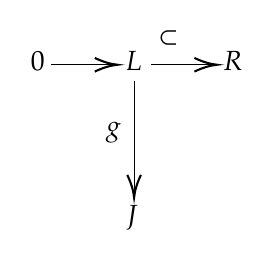
\begin{tikzpicture}[x=0.75pt,y=0.75pt,yscale=-1,xscale=1]
%uncomment if require: \path (0,476); %set diagram left start at 0, and has height of 476

%Straight Lines [id:da2979778987226902] 
\draw    (232,120) -- (262,120) ;
\draw [shift={(264,120)}, rotate = 180] [color={rgb, 255:red, 0; green, 0; blue, 0 }  ][line width=0.75]    (10.93,-3.29) .. controls (6.95,-1.4) and (3.31,-0.3) .. (0,0) .. controls (3.31,0.3) and (6.95,1.4) .. (10.93,3.29)   ;
%Straight Lines [id:da1283630480544964] 
\draw    (280,120) -- (310,120) ;
\draw [shift={(312,120)}, rotate = 180] [color={rgb, 255:red, 0; green, 0; blue, 0 }  ][line width=0.75]    (10.93,-3.29) .. controls (6.95,-1.4) and (3.31,-0.3) .. (0,0) .. controls (3.31,0.3) and (6.95,1.4) .. (10.93,3.29)   ;
%Straight Lines [id:da5874779160595505] 
\draw    (272,128) -- (272,182) ;
\draw [shift={(272,184)}, rotate = 270] [color={rgb, 255:red, 0; green, 0; blue, 0 }  ][line width=0.75]    (10.93,-3.29) .. controls (6.95,-1.4) and (3.31,-0.3) .. (0,0) .. controls (3.31,0.3) and (6.95,1.4) .. (10.93,3.29)   ;

% Text Node
\draw (221,112.4) node [anchor=north west][inner sep=0.75pt]    {$0$};
% Text Node
\draw (267,112.4) node [anchor=north west][inner sep=0.75pt]    {$L$};
% Text Node
\draw (314,112.4) node [anchor=north west][inner sep=0.75pt]    {$R$};
% Text Node
\draw (267,186.4) node [anchor=north west][inner sep=0.75pt]    {$J$};
% Text Node
\draw (283,102.4) node [anchor=north west][inner sep=0.75pt]    {$\subset $};
% Text Node
\draw (257,146.4) node [anchor=north west][inner sep=0.75pt]    {$g$};


\end{tikzpicture}
\end{center}
Now since $J$ is an injective module over $\mathbb{Z}$, there exists some extension of $g$, denote as $\overline{g}:R\to J$. We now define $h:R\to\mathrm{Hom}_\mathbb{Z}(R,J)$ to be $r\mapsto h(r)$, where $h(r)(x)=\overline{g}(xr)$. It is easy to verify that $h(r)\in\mathrm{Hom}_\mathbb{Z}(R,J)$ and hence $h:R\to\mathrm{Hom}_\mathbb{Z}(R,J)$. Now suppose $r\in L$ and $x\in R$. Then $xr\in L$ and 
$$
h\left( r \right) \left( x \right) =\overline{g}\left( xr \right) =g\left( xr \right) =\left[ f\left( xr \right) \right] 1_R=\left[ xf\left( r \right) \right] 1_R=f\left( r \right) \left( 1_Rx \right) =f\left( r \right) \left( x \right) ,
$$
therefore $h(r)=f(r)$, and the proof is finished.
\end{proof}
We are now able to proof the duals of Corollary 5.28 and Theorem 5.29.
\begin{proposition}
Every unitary module $A$ over a ring $R$ with identity may be embedded in an injective $R$-module.
\end{proposition}
\begin{proof}
First since $A$ is an abelian group, there exists some divisible abelian groups $J$ such that $A$ may be embedded in $J$. Define the $R$-module monomorphism $f:A\to J$. Then we consider $\overline{f}:\mathrm{Hom}_\mathbb{Z}(R,A)\to\mathrm{Hom}_\mathbb{Z}(R,J)$ given by $g\mapsto fg$, where $g\in\mathrm{Hom}_\mathbb{Z}(R,A)$. It is easy to verify that $\overline{f}$ is also an $R$-module monomorphism. Note that every $R$-module homomorphism is also a $\mathbb{Z}$-module homomorphism, which due to the fact that every $R$-module is an abelian group, and hence a $\mathbb{Z}$-module, we obtain the inclusion $\mathrm{Hom}_R(R,A)\subset\mathrm{Hom}_\mathbb{Z}(R,A)$. Observe that $A$ may be embedded into $\mathrm{Hom}_R(R,A)$, which suffices to note that the map $g:A\to\mathrm{Hom}_R(R,A)$ given by $a\mapsto f_a$, where $f_a$ is defined to be $f_a(r)=ra$, is a monomorphism, we have the following composition: 
$$
A\overset{g}{\longrightarrow}\mathrm{Hom}_R\left( R,A \right) \overset{\subset}{\longrightarrow}\mathrm{Hom}_{\mathbb{Z}}\left( R,A \right) \overset{\overline{f}}{\longrightarrow}\mathrm{Hom}_{\mathbb{Z}}\left( R,J \right) ,
$$
we conclude that $A$ may be embedded into $\mathrm{Hom}_\mathbb{Z}(R,J)$, where the latter one is, by Lemma 5.7, an injective $R$-module.
\end{proof}
\begin{proposition}
Let $R$ be a ring with identity. The following conditions on a unitary $R$-module $J$ are equivalent.\par
(a) $J$ is injective;\par
(b) every short exact sequence $0\longrightarrow J\overset{f}{\longrightarrow}B\overset{g}{\longrightarrow}C\longrightarrow 0$ is split exact;\par
(c) $J$ is the direct summand of any module $B$ of which it is a submodule.
\end{proposition}
\begin{proof}
(a)$\Rightarrow$(b): Dualize the proof of Theorem 5.29.\par
(b)$\Rightarrow$(c): Consider the short exact sequence 
$$
0\longrightarrow J\overset{\subset}{\longrightarrow}B\overset{\pi}{\longrightarrow}B/J\longrightarrow 0,
$$
therefore since the short exact sequence is split exact, we have $B\cong J\oplus B/J$, whence $J$ is a direct summand of $B$.\par
(c)$\Rightarrow$(a): It follows from Proposition 5.33 that $J$ is a submodule of some injective module $Q$. Proposition 5.32 and (c) implies that $J$ is injective.
\end{proof}
\begin{center}
\begin{large}
    \textbf{Exercises for 5.3}
\end{large}
\end{center}
Note: $R$ is a ring. If $R$ has an identity, all $R$-modules are assumed to be unitary.
\begin{problem}\em
The following conditions on a ring $R$ [with identity] are equivalent:\par
(a) Every [unitary] $R$-module is projective.\par
(b) Every short exact sequence of [unitary] $R$-modules is split exact.\par
(c) Every [unitary] $R$-module is injective.
\end{problem}
\begin{proof}
We first show that (a) and (b) are equivalent.\par
(a)$\Rightarrow$(b): Note that the following diagram 
\begin{center}


\tikzset{every picture/.style={line width=0.75pt}} %set default line width to 0.75pt        

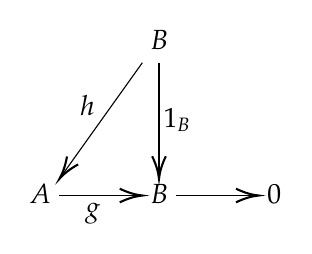
\begin{tikzpicture}[x=0.75pt,y=0.75pt,yscale=-1,xscale=1]
%uncomment if require: \path (0,476); %set diagram left start at 0, and has height of 476

%Straight Lines [id:da22892850871398007] 
\draw    (208,192) -- (246,192) ;
\draw [shift={(248,192)}, rotate = 180] [color={rgb, 255:red, 0; green, 0; blue, 0 }  ][line width=0.75]    (10.93,-3.29) .. controls (6.95,-1.4) and (3.31,-0.3) .. (0,0) .. controls (3.31,0.3) and (6.95,1.4) .. (10.93,3.29)   ;
%Straight Lines [id:da815882418865653] 
\draw    (264,192) -- (302,192) ;
\draw [shift={(304,192)}, rotate = 180] [color={rgb, 255:red, 0; green, 0; blue, 0 }  ][line width=0.75]    (10.93,-3.29) .. controls (6.95,-1.4) and (3.31,-0.3) .. (0,0) .. controls (3.31,0.3) and (6.95,1.4) .. (10.93,3.29)   ;
%Straight Lines [id:da20936486711467128] 
\draw    (256,128) -- (256,182) ;
\draw [shift={(256,184)}, rotate = 270] [color={rgb, 255:red, 0; green, 0; blue, 0 }  ][line width=0.75]    (10.93,-3.29) .. controls (6.95,-1.4) and (3.31,-0.3) .. (0,0) .. controls (3.31,0.3) and (6.95,1.4) .. (10.93,3.29)   ;
%Straight Lines [id:da9215006364241813] 
\draw    (248,128) -- (209.16,182.37) ;
\draw [shift={(208,184)}, rotate = 305.54] [color={rgb, 255:red, 0; green, 0; blue, 0 }  ][line width=0.75]    (10.93,-3.29) .. controls (6.95,-1.4) and (3.31,-0.3) .. (0,0) .. controls (3.31,0.3) and (6.95,1.4) .. (10.93,3.29)   ;

% Text Node
\draw (193,185.4) node [anchor=north west][inner sep=0.75pt]    {$A$};
% Text Node
\draw (251,185.4) node [anchor=north west][inner sep=0.75pt]    {$B$};
% Text Node
\draw (307,185.4) node [anchor=north west][inner sep=0.75pt]    {$0$};
% Text Node
\draw (251,111.4) node [anchor=north west][inner sep=0.75pt]    {$B$};
% Text Node
\draw (257,148.4) node [anchor=north west][inner sep=0.75pt]    {$1_{B}$};
% Text Node
\draw (219,194.4) node [anchor=north west][inner sep=0.75pt]    {$g$};
% Text Node
\draw (217,142.4) node [anchor=north west][inner sep=0.75pt]    {$h$};


\end{tikzpicture}
\end{center}
is commutative, there exists some $h:B\to A$ and hence the short exact sequence is split exact.\par
(b)$\Rightarrow$(a): Since every short exact sequence of $R$-modules is split exact, then the short exact sequence 
$$
0\longrightarrow A\overset{f}{\longrightarrow}B\overset{g}{\longrightarrow}P\longrightarrow 0
$$
is split exact, hence $P$ is a projective module.\par
We now show that (b) and (c) are equivalent, and hence the proof is finished.\par
(b)$\Rightarrow$(c): Since every short exact sequence of $R$-modules is split exact, then the short exact sequence 
$$
0\longrightarrow J\overset{f}{\longrightarrow}A\overset{g}{\longrightarrow}B\longrightarrow 0
$$
is split exact, hence $J$ is an injective module.\par
(c)$\Rightarrow$(b): Note that the following diagram 
\begin{center}


\tikzset{every picture/.style={line width=0.75pt}} %set default line width to 0.75pt        

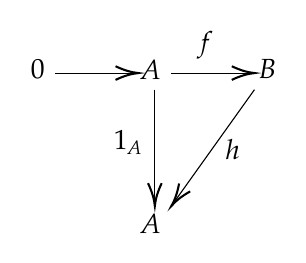
\begin{tikzpicture}[x=0.75pt,y=0.75pt,yscale=-1,xscale=1]
%uncomment if require: \path (0,476); %set diagram left start at 0, and has height of 476

%Straight Lines [id:da5937754556996264] 
\draw    (200,112) -- (238,112) ;
\draw [shift={(240,112)}, rotate = 180] [color={rgb, 255:red, 0; green, 0; blue, 0 }  ][line width=0.75]    (10.93,-3.29) .. controls (6.95,-1.4) and (3.31,-0.3) .. (0,0) .. controls (3.31,0.3) and (6.95,1.4) .. (10.93,3.29)   ;
%Straight Lines [id:da0029257347153581748] 
\draw    (256,112) -- (294,112) ;
\draw [shift={(296,112)}, rotate = 180] [color={rgb, 255:red, 0; green, 0; blue, 0 }  ][line width=0.75]    (10.93,-3.29) .. controls (6.95,-1.4) and (3.31,-0.3) .. (0,0) .. controls (3.31,0.3) and (6.95,1.4) .. (10.93,3.29)   ;
%Straight Lines [id:da8317479595227399] 
\draw    (248,120) -- (248,174) ;
\draw [shift={(248,176)}, rotate = 270] [color={rgb, 255:red, 0; green, 0; blue, 0 }  ][line width=0.75]    (10.93,-3.29) .. controls (6.95,-1.4) and (3.31,-0.3) .. (0,0) .. controls (3.31,0.3) and (6.95,1.4) .. (10.93,3.29)   ;
%Straight Lines [id:da6461060090515085] 
\draw    (296,120) -- (257.16,174.37) ;
\draw [shift={(256,176)}, rotate = 305.54] [color={rgb, 255:red, 0; green, 0; blue, 0 }  ][line width=0.75]    (10.93,-3.29) .. controls (6.95,-1.4) and (3.31,-0.3) .. (0,0) .. controls (3.31,0.3) and (6.95,1.4) .. (10.93,3.29)   ;

% Text Node
\draw (187,104.4) node [anchor=north west][inner sep=0.75pt]    {$0$};
% Text Node
\draw (240,104.4) node [anchor=north west][inner sep=0.75pt]    {$A$};
% Text Node
\draw (297,104.4) node [anchor=north west][inner sep=0.75pt]    {$B$};
% Text Node
\draw (240,178.4) node [anchor=north west][inner sep=0.75pt]    {$A$};
% Text Node
\draw (267,90.4) node [anchor=north west][inner sep=0.75pt]    {$f$};
% Text Node
\draw (281,142.4) node [anchor=north west][inner sep=0.75pt]    {$h$};
% Text Node
\draw (227,138.4) node [anchor=north west][inner sep=0.75pt]    {$1_{A}$};


\end{tikzpicture}
\end{center}
is commutative, there exists some $h:B\to A$ and hence the short exact sequence is split exact.
\end{proof}
\begin{problem}\em
Let $R$ be a ring with identity. An $R$-module $A$ is injective if and only if for every left ideal $L$ of $R$ and $R$-module homomorphism $g:L\to A$, there exists $a\in A$ such that $g(r)=ra$ for every $r\in L$.
\end{problem}
\begin{proof}
Suppose $A$ is an injective $R$-module, then there exists an extension $h:R\to A$ of $g$, hence 
$$
g\left( r \right) =h\left( r \right) =h\left( r\cdot 1_R \right) =h\left( 1_R \right) r,
$$
let $h(1_R)=a$. Conversely, since $L$ is an ideal of $R$, we have $rl\in L$ for all $r\in R$ and $l\in L$. Therefore $g\left( rl \right) =rg\left( l \right) =rla$ defines an extension of $g$, and hence $A$ is injective.
\end{proof}
\begin{problem}\em
Every vector space over a division ring $D$ is both a projective and injective $D$-module.
\end{problem}
\begin{proof}
Since every vector space has a basis, we know that $V$ is a free $D$-module, therefore a projective module. By Exercise 5.26 we know that $V$ is also an injective module.
\end{proof}
\begin{problem}\em
(a) For each prime $p$, $\mathbb{Z}(p^\infty)$ is a divisible group.\par
(b) No nonzero finite abelian group is divisible.\par
(c) No nonzero free abelian group is divisible.\par
(d) $\mathbb{Q}$ is an injective $\mathbb{Z}$-module.
\end{problem}
\begin{proof}
(a) Let $\overline{a/p^l}\in\mathbb{Z}(p^\infty)$ and $n\in\mathbb{Z}$ an integer. We show that there exists some $y\in\mathbb{Z}(p^\infty)$ such that $ny=x$. Suppose $n=p^mr$. Then $r$ is an invertible element in $\mathbb{Z}/p^i\mathbb{Z}$ since $(r,p)=1$, whence there exists some $s\in\mathbb{Z}$ such that $rs\equiv 1(\mathrm{mod}p^i)$. Let $y=\overline{as/p^{m+l}}$, then 
$$
ny=n\cdot \overline{as/p^{m+l}}=p^mr\cdot \overline{as/p^{m+l}}=\overline{ars/p^l}=\overline{a/p^l}=x,
$$
whence $\mathbb{Z}(p^\infty)$ is divisible.\par
(b) Suppose $A$ is a finite abelian group. Then $A\cong\bigoplus\mathbb{Z}/p^i\mathbb{Z}$ for some prime $p$ and $i\in\mathbb{Z}$. We show that $\mathbb{Z}/p^i\mathbb{Z}$ are not injective modules. Consider the short exact sequence 
$$
0\longrightarrow p^i\mathbb{Z} /p^{2i}\mathbb{Z} \longrightarrow \mathbb{Z} /p^{2i}\mathbb{Z} \longrightarrow \mathbb{Z} /p^i\mathbb{Z} \longrightarrow 0
$$
where each homomorphism is the canonical injection. It is not spilt exact since 
$$
\mathbb{Z} /p^{2i}\mathbb{Z} \ncong p^i\mathbb{Z} /p^{2i}\mathbb{Z} \oplus \mathbb{Z} /p^i\mathbb{Z} ,
$$
whence $\mathbb{Z}/p^i\mathbb{Z}$ is not injective $\mathbb{Z}$-module, so is $A$.\par
(c) Suppose $F$ is a free abelian group. Then $F\cong\bigoplus\mathbb{Z}$. We show that $\mathbb{Z}$ is not an injective $\mathbb{Z}$-module. Consider the short exact sequence 
$$
0\longrightarrow \mathbb{Z} \longrightarrow \mathbb{Z} \oplus 2\mathbb{Z} \longrightarrow \mathbb{Z} \longrightarrow 0
$$
with the first arrow canonical injection and the second $2k\mapsto k$. It is not split exact since 
$$
\mathbb{Z} \oplus 2\mathbb{Z} \ncong \mathbb{Z} \oplus \mathbb{Z} .
$$
Therefore $F$ is not an injective $\mathbb{Z}$-module.\par
(d) We proof by using Exercise 5.27. Consider a $\mathbb{Z}$-module homomorphism $g:n\mathbb{Z}\to\mathbb{Q}$, where $n\mathbb{Z}$ is an ideal of $\mathbb{Z}$. Since $\mathbb{Q}$ is divisible, there exists some $y\in\mathbb{Q}$ such that $ky=g(k)$ for all $k\in n\mathbb{Z}$. Therefore $g$ may be extended onto $\mathbb{Z}$ and hence $\mathbb{Q}$ an injective $\mathbb{Z}$-module.
\end{proof}
\begin{problem}\em
$\mathbb{Q}$ is not projective $\mathbb{Z}$-module.
\end{problem}
\begin{proof}
Note that a module is projective over principal ideal domain if and only if it is free (which will be introduced in section 5.6), if $\mathbb{Q}$ is projective, then $\mathbb{Q}$ is a free $\mathbb{Z}$-module. However $\mathbb{Q}$ is not free over $\mathbb{Z}$, a contradiction!
\end{proof}
\begin{problem}\em
If $G$ is an abelian group, then $G\cong D\oplus N$, with $D$ divisible and $N$ \textbf{reduced}, i.e., $N$ has no nontrivial divisible subgroups.
\end{problem}
\begin{proof}
Suppose $\{D_i\}_{i\in I}$ is the collection of all subgroups of $G$ such that $D_i$ is divisible, and let $D=\left<\bigcup_{i\in I}D_i\right>$. Since $G$ is an abelian group, we have $D\lhd G$. Let $N=G/D$, then $G\cong D\oplus N$, we finished the proof.
\end{proof}
\begin{problem}\em
Every torsion-free divisible abelian group $D$ is a direct sum of copies of the rationals $\mathbb{Q}$.
\end{problem}
\begin{proof}
We show that $D$ is a vector space over $\mathbb{Q}$. To see this, observe that $D$ is divisible, hence for all $x\in D$, there exists some $y\in D$ such that $ny=x$. Denote $y=(1/n)x$ and $my=(m/n)x$. Since $D$ is torsion-free, we have $r_1x=r_2x$ if and only if $r_1=r_2$. By easy verification of definition one may show that $D$ is a vector space over $\mathbb{Q}$, whence $D$ has a basis $X$. Suppose $r\in D$ and $r=\sum_{i\in I}k_ix_i$, where $r_i\in X$ and $k_i\in\mathbb{Q}$, therefore there exists a correspondence that $r\mapsto(k_1,k_2,\cdots)\in\bigoplus_{i\in I}\mathbb{Q}$. Since the correspondence is one-to-one, we showed that $D\cong\bigoplus\mathbb{Q}$.
\end{proof}
\begin{problem}\em
(a) If $D$ is an abelian group with torsion subgroup $D_t$, then $D/D_t$ is torsion free.\par
(b) If $D$ is divisible, then so is $D_t$, whence $D\cong D_t\oplus E$, where $E$ is torsion free.
\end{problem}
\begin{proof}
(a) Suppose $a+D_t\in D/D_t$. If $a+D_t$ has finite order, then there exists some $n\in\mathbb{Z}$ such that $na+D_t=0+D_t$, whence $na\in D_t$. Since $D_t$ is torsion group, there exists some $m\in\mathbb{Z}$ such that $mna=0$, whence $a\in D_t$ and hence $a+D_t=0+D_t$.\par
(b) Suppose $D$ is divisible. Let $y\in D_t$. Since $D_t$ is a subgroup of $D$ and $D$ is divisible, there exists some $x\in D$ such that $nx=y$ with $n\in\mathbb{Z}$. However $y\in D_t$, whence $my=0$ for some $m\in\mathbb{Z}$, hence $mnx=0$, whence $x\in D_t$ and this implies $D_t$ divisible. By Exercise 5.31 we finished the proof.
\end{proof}
\begin{problem}\em
Let $p$ be a prime and $D$ a divisible abelian $p$-group. Then $D$ is a direct sum of copies of $\mathbb{Z}(p^\infty)$.
\end{problem}
\begin{proof}
We consider $D[p]$ as a vector space of $\mathbb{Z}/(p)=\mathbb{Z}_p$, see exercise 5.18. Let $X$ be the basis of $D[p]$. Since $D$ is a divisible abelian $p$-group, then for all $x\in X$, there exists some $x_1\in X$ such that $|x_1|=p$. Now since $D$ is divisible, there exists some $x_2=px_1,\cdots,x_{n+1}=px_n,\cdots$. Now suppose $H_x$ is generated by $x_1,x_2,\cdots$, by Exercise 2.36 we have $H_x\cong\mathbb{Z}(p^\infty)$. Therefore $D\cong\bigoplus H_x\cong\bigoplus\mathbb{Z}(p^\infty)$.
\end{proof}
\begin{problem}\em
Every divisible abelian group is a direct sum of copies of the rationals $\mathbb{Q}$ and copies of $\mathbb{Z}(p^\infty)$ for various primes $p$.
\end{problem}
\begin{proof}
Let $G_t$ be a torsion subgroup of $G$, then $G_t$ is divisible. Hence by Exercise 5.33 there exists some $E$ that is torsion-free such that $G\cong G_t\oplus E$. For $E$, it is divisible and torsion-free, therefore by Exercise 5.32 we know that $E\cong\bigoplus\mathbb{Q}$. Now for $G_t$, since it is a torsion group, it is the direct sum of some $p$-groups. By Exercise 5.34 we know that each $p$-group is the direct sum of some $\mathbb{Z}(p^\infty)$, therefore 
$$
G\cong G_t\oplus E\cong \left( \bigoplus_{p\in \mathcal{P}}{G_p} \right) \oplus \left( \bigoplus{\mathbb{Q}} \right) \cong \left( \bigoplus_{p\in \mathcal{P}}{\mathbb{Z} \left( p^{\infty} \right)} \right) \oplus \left( \bigoplus{\mathbb{Q}} \right) ,
$$
which finished the proof.
\end{proof}
\begin{problem}\em
Let $G,H,K$ be divisible abelian groups.\par
(a) If $G\oplus G\cong H\oplus H$, then $G\cong H$.\par
(b) If $G\oplus K\cong H\oplus K$, then $H\cong K$.
\end{problem}
\begin{proof}
(a) By Exercise 5.35, this is trivial.\par
(b) By Exercise 5.35, we may deduce the consequence into that of finite abelian groups, whence the proof is finished.
\end{proof}
\subsection{Hom and Duality}
Recall that if $A$ and $B$ are modules over a ring $R$, then $\mathrm{Hom}_R(A,B)$ is the set of all $R$-module homomorphisms $f:A\to B$. If $R=\mathbb{Z}$ we shall usually write $\mathrm{Hom}(A,B)$ rather than $\mathrm{Hom}_\mathbb{Z}(A,B)$. $\mathrm{Hom}_R(A,B)$ is an abelian group under addition and this addition is distributive with respect to composition of functions.
\begin{theorem}
Let $A,B,C,D$ be modules over a ring $R$ and $\varphi:C\to A$ and $\psi:B\to D$ $R$-module homomorphisms. Then the map $\theta:\mathrm{Hom}_R(A,B)\to\mathrm{Hom}_R(C,D)$ given by $f\mapsto\psi f\varphi$ is a homomorphism of abelian groups.
\end{theorem}
\begin{proof}
The map $\theta$ is first well-defined since composition of $R$-module homomorphisms is a homomorphism. It is then an $R$-module homomorphism since the composition of homomorphisms is distributive with respect to addition.
\end{proof}
The homomorphism $\theta$ is usually denoted $\mathrm{Hom}(\varphi,\psi)$ and called homomorphism induced by $\varphi$ and $\psi$, see the following diagram:
\begin{center}


\tikzset{every picture/.style={line width=0.75pt}} %set default line width to 0.75pt        

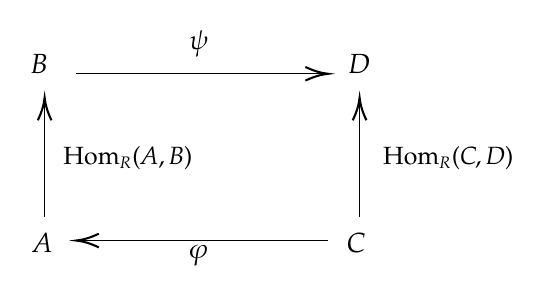
\begin{tikzpicture}[x=0.75pt,y=0.75pt,yscale=-1,xscale=1]
%uncomment if require: \path (0,476); %set diagram left start at 0, and has height of 476

%Straight Lines [id:da2920246208679915] 
\draw    (191.18,237.57) -- (191.18,182.17) ;
\draw [shift={(191.18,180.17)}, rotate = 90] [color={rgb, 255:red, 0; green, 0; blue, 0 }  ][line width=0.75]    (10.93,-3.29) .. controls (6.95,-1.4) and (3.31,-0.3) .. (0,0) .. controls (3.31,0.3) and (6.95,1.4) .. (10.93,3.29)   ;
%Straight Lines [id:da04506002983020263] 
\draw    (342.93,237.57) -- (342.93,182.17) ;
\draw [shift={(342.93,180.17)}, rotate = 90] [color={rgb, 255:red, 0; green, 0; blue, 0 }  ][line width=0.75]    (10.93,-3.29) .. controls (6.95,-1.4) and (3.31,-0.3) .. (0,0) .. controls (3.31,0.3) and (6.95,1.4) .. (10.93,3.29)   ;
%Straight Lines [id:da37803238364229985] 
\draw    (206.35,168.7) -- (325.75,168.7) ;
\draw [shift={(327.75,168.7)}, rotate = 180] [color={rgb, 255:red, 0; green, 0; blue, 0 }  ][line width=0.75]    (10.93,-3.29) .. controls (6.95,-1.4) and (3.31,-0.3) .. (0,0) .. controls (3.31,0.3) and (6.95,1.4) .. (10.93,3.29)   ;
%Straight Lines [id:da5428498747387094] 
\draw    (327.75,249.04) -- (208.35,249.04) ;
\draw [shift={(206.35,249.04)}, rotate = 360] [color={rgb, 255:red, 0; green, 0; blue, 0 }  ][line width=0.75]    (10.93,-3.29) .. controls (6.95,-1.4) and (3.31,-0.3) .. (0,0) .. controls (3.31,0.3) and (6.95,1.4) .. (10.93,3.29)   ;

% Text Node
\draw (183.28,158.23) node [anchor=north west][inner sep=0.75pt]    {$B$};
% Text Node
\draw (336.38,158.23) node [anchor=north west][inner sep=0.75pt]    {$D$};
% Text Node
\draw (184.18,244.31) node [anchor=north west][inner sep=0.75pt]    {$A$};
% Text Node
\draw (335.48,244.31) node [anchor=north west][inner sep=0.75pt]    {$C$};
% Text Node
\draw (259.6,250.05) node [anchor=north west][inner sep=0.75pt]    {$\varphi $};
% Text Node
\draw (259.6,146.75) node [anchor=north west][inner sep=0.75pt]    {$\psi $};
% Text Node
\draw (199,202.4) node [anchor=north west][inner sep=0.75pt]  [font=\small]  {$\text{Hom}_{R}( A,B)$};
% Text Node
\draw (353,202.4) node [anchor=north west][inner sep=0.75pt]  [font=\small]  {$\text{Hom}_{R}( C,D)$};


\end{tikzpicture}
\end{center}
The composition of $\mathrm{Hom}(\varphi_1,\psi_2)$ and $\mathrm{Hom}(\varphi_2,\psi_1)$, as defined in the diagram, 
\begin{center}


\tikzset{every picture/.style={line width=0.75pt}} %set default line width to 0.75pt        

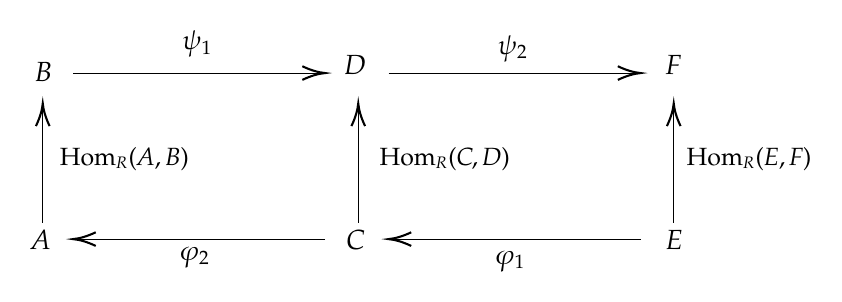
\begin{tikzpicture}[x=0.75pt,y=0.75pt,yscale=-1,xscale=1]
%uncomment if require: \path (0,476); %set diagram left start at 0, and has height of 476

%Straight Lines [id:da2920246208679915] 
\draw    (192,240) -- (192,184.61) ;
\draw [shift={(192,182.61)}, rotate = 90] [color={rgb, 255:red, 0; green, 0; blue, 0 }  ][line width=0.75]    (10.93,-3.29) .. controls (6.95,-1.4) and (3.31,-0.3) .. (0,0) .. controls (3.31,0.3) and (6.95,1.4) .. (10.93,3.29)   ;
%Straight Lines [id:da04506002983020263] 
\draw    (344,240) -- (344,184.61) ;
\draw [shift={(344,182.61)}, rotate = 90] [color={rgb, 255:red, 0; green, 0; blue, 0 }  ][line width=0.75]    (10.93,-3.29) .. controls (6.95,-1.4) and (3.31,-0.3) .. (0,0) .. controls (3.31,0.3) and (6.95,1.4) .. (10.93,3.29)   ;
%Straight Lines [id:da37803238364229985] 
\draw    (206.6,168) -- (326,168) ;
\draw [shift={(328,168)}, rotate = 180] [color={rgb, 255:red, 0; green, 0; blue, 0 }  ][line width=0.75]    (10.93,-3.29) .. controls (6.95,-1.4) and (3.31,-0.3) .. (0,0) .. controls (3.31,0.3) and (6.95,1.4) .. (10.93,3.29)   ;
%Straight Lines [id:da5428498747387094] 
\draw    (328,248) -- (208.6,248) ;
\draw [shift={(206.6,248)}, rotate = 360] [color={rgb, 255:red, 0; green, 0; blue, 0 }  ][line width=0.75]    (10.93,-3.29) .. controls (6.95,-1.4) and (3.31,-0.3) .. (0,0) .. controls (3.31,0.3) and (6.95,1.4) .. (10.93,3.29)   ;
%Straight Lines [id:da0021870933535605985] 
\draw    (358.6,168) -- (478,168) ;
\draw [shift={(480,168)}, rotate = 180] [color={rgb, 255:red, 0; green, 0; blue, 0 }  ][line width=0.75]    (10.93,-3.29) .. controls (6.95,-1.4) and (3.31,-0.3) .. (0,0) .. controls (3.31,0.3) and (6.95,1.4) .. (10.93,3.29)   ;
%Straight Lines [id:da9085135985503727] 
\draw    (480,248) -- (360.6,248) ;
\draw [shift={(358.6,248)}, rotate = 360] [color={rgb, 255:red, 0; green, 0; blue, 0 }  ][line width=0.75]    (10.93,-3.29) .. controls (6.95,-1.4) and (3.31,-0.3) .. (0,0) .. controls (3.31,0.3) and (6.95,1.4) .. (10.93,3.29)   ;
%Straight Lines [id:da06661859833245565] 
\draw    (496,240) -- (496,184.61) ;
\draw [shift={(496,182.61)}, rotate = 90] [color={rgb, 255:red, 0; green, 0; blue, 0 }  ][line width=0.75]    (10.93,-3.29) .. controls (6.95,-1.4) and (3.31,-0.3) .. (0,0) .. controls (3.31,0.3) and (6.95,1.4) .. (10.93,3.29)   ;

% Text Node
\draw (187,161.4) node [anchor=north west][inner sep=0.75pt]    {$B$};
% Text Node
\draw (336,158.4) node [anchor=north west][inner sep=0.75pt]    {$D$};
% Text Node
\draw (185,242.4) node [anchor=north west][inner sep=0.75pt]    {$A$};
% Text Node
\draw (337,242.4) node [anchor=north west][inner sep=0.75pt]    {$C$};
% Text Node
\draw (257,250.4) node [anchor=north west][inner sep=0.75pt]    {$\varphi _{2}$};
% Text Node
\draw (258,146.4) node [anchor=north west][inner sep=0.75pt]    {$\psi _{1}$};
% Text Node
\draw (199,202.4) node [anchor=north west][inner sep=0.75pt]  [font=\small]  {$\text{Hom}_{R}( A,B)$};
% Text Node
\draw (353,202.4) node [anchor=north west][inner sep=0.75pt]  [font=\small]  {$\text{Hom}_{R}( C,D)$};
% Text Node
\draw (491,242.4) node [anchor=north west][inner sep=0.75pt]    {$E$};
% Text Node
\draw (491,158.4) node [anchor=north west][inner sep=0.75pt]    {$F$};
% Text Node
\draw (410,148.4) node [anchor=north west][inner sep=0.75pt]    {$\psi _{2}$};
% Text Node
\draw (409,252.4) node [anchor=north west][inner sep=0.75pt]    {$\varphi _{1}$};
% Text Node
\draw (501,202.4) node [anchor=north west][inner sep=0.75pt]  [font=\small]  {$\text{Hom}_{R}( E,F)$};


\end{tikzpicture}
\end{center}
is as follows: 
$$
\mathrm{Hom}\left( \varphi _1,\psi _2 \right) \mathrm{Hom}\left( \varphi _2,\psi _1 \right) =\mathrm{Hom}\left( \varphi _2\varphi _1,\psi _2\psi _1 \right) :\mathrm{Hom}_R\left( A,B \right) \rightarrow \mathrm{Hom}_R\left( E,F \right) .
$$
There are two special cases of the induced homomorphism. If $B=D$ and $\psi=1_B$, then the induced map $\mathrm{Hom}(\varphi,1_B)$ is given by $f\mapsto f\varphi$ and is denoted $\overline{\varphi}$. Similarly if $A=C$ and $\varphi=1_A$ the induced map $\mathrm{Hom}(1_A,\psi)$ is given by $f\mapsto\psi f$ and is denoted $\overline{\psi}$. The diagram in this case is presented below: 
\begin{center}


\tikzset{every picture/.style={line width=0.75pt}} %set default line width to 0.75pt        

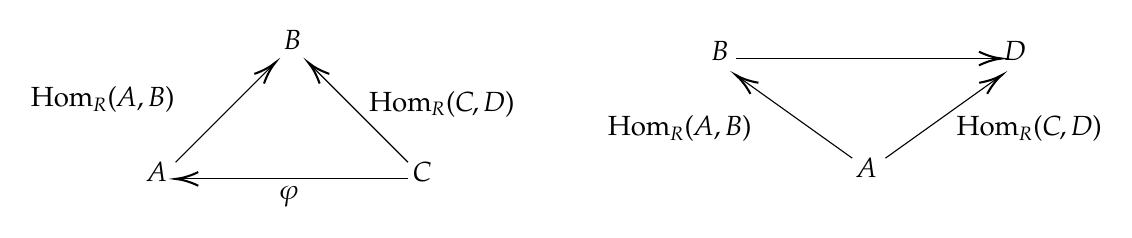
\begin{tikzpicture}[x=0.75pt,y=0.75pt,yscale=-1,xscale=1]
%uncomment if require: \path (0,476); %set diagram left start at 0, and has height of 476

%Straight Lines [id:da597002119082159] 
\draw    (264,235) -- (154,235) ;
\draw [shift={(152,235)}, rotate = 360] [color={rgb, 255:red, 0; green, 0; blue, 0 }  ][line width=0.75]    (10.93,-3.29) .. controls (6.95,-1.4) and (3.31,-0.3) .. (0,0) .. controls (3.31,0.3) and (6.95,1.4) .. (10.93,3.29)   ;
%Straight Lines [id:da1798127284338633] 
\draw    (152,227) -- (198.59,180.41) ;
\draw [shift={(200,179)}, rotate = 135] [color={rgb, 255:red, 0; green, 0; blue, 0 }  ][line width=0.75]    (10.93,-3.29) .. controls (6.95,-1.4) and (3.31,-0.3) .. (0,0) .. controls (3.31,0.3) and (6.95,1.4) .. (10.93,3.29)   ;
%Straight Lines [id:da051057573396247724] 
\draw    (264,227) -- (217.41,180.41) ;
\draw [shift={(216,179)}, rotate = 45] [color={rgb, 255:red, 0; green, 0; blue, 0 }  ][line width=0.75]    (10.93,-3.29) .. controls (6.95,-1.4) and (3.31,-0.3) .. (0,0) .. controls (3.31,0.3) and (6.95,1.4) .. (10.93,3.29)   ;
%Straight Lines [id:da31040695645518945] 
\draw    (478,225) -- (423.63,186.16) ;
\draw [shift={(422,185)}, rotate = 35.54] [color={rgb, 255:red, 0; green, 0; blue, 0 }  ][line width=0.75]    (10.93,-3.29) .. controls (6.95,-1.4) and (3.31,-0.3) .. (0,0) .. controls (3.31,0.3) and (6.95,1.4) .. (10.93,3.29)   ;
%Straight Lines [id:da054410057315041005] 
\draw    (422,177) -- (548,177) ;
\draw [shift={(550,177)}, rotate = 180] [color={rgb, 255:red, 0; green, 0; blue, 0 }  ][line width=0.75]    (10.93,-3.29) .. controls (6.95,-1.4) and (3.31,-0.3) .. (0,0) .. controls (3.31,0.3) and (6.95,1.4) .. (10.93,3.29)   ;
%Straight Lines [id:da5548694030859183] 
\draw    (494,225) -- (548.37,186.16) ;
\draw [shift={(550,185)}, rotate = 144.46] [color={rgb, 255:red, 0; green, 0; blue, 0 }  ][line width=0.75]    (10.93,-3.29) .. controls (6.95,-1.4) and (3.31,-0.3) .. (0,0) .. controls (3.31,0.3) and (6.95,1.4) .. (10.93,3.29)   ;

% Text Node
\draw (137,225.4) node [anchor=north west][inner sep=0.75pt]    {$A$};
% Text Node
\draw (265,225.4) node [anchor=north west][inner sep=0.75pt]    {$C$};
% Text Node
\draw (203,162.4) node [anchor=north west][inner sep=0.75pt]    {$B$};
% Text Node
\draw (201,237.4) node [anchor=north west][inner sep=0.75pt]    {$\varphi $};
% Text Node
\draw (81,189.4) node [anchor=north west][inner sep=0.75pt]    {$\text{Hom}_{R}( A,B)$};
% Text Node
\draw (244,191.4) node [anchor=north west][inner sep=0.75pt]    {$\text{Hom}_{R}( C,D)$};
% Text Node
\draw (479,223.4) node [anchor=north west][inner sep=0.75pt]    {$A$};
% Text Node
\draw (550,167.4) node [anchor=north west][inner sep=0.75pt]    {$D$};
% Text Node
\draw (409,167.4) node [anchor=north west][inner sep=0.75pt]    {$B$};
% Text Node
\draw (359,203.4) node [anchor=north west][inner sep=0.75pt]    {$\text{Hom}_{R}( A,B)$};
% Text Node
\draw (527,203.4) node [anchor=north west][inner sep=0.75pt]    {$\text{Hom}_{R}( C,D)$};


\end{tikzpicture}
\end{center}
We now examine the behavior of $\mathrm{Hom}_R$ with respect to exact sequences.
\begin{theorem}
Let $R$ be a ring. $0\longrightarrow A\overset{\varphi}{\longrightarrow}B\overset{\psi}{\longrightarrow}C$ is an exact sequence of $R$-modules if and only if for every $R$-module $D$ 
$$
0\longrightarrow \mathrm{Hom}_R\left( D,A \right) \overset{\overline{\varphi }}{\longrightarrow}\mathrm{Hom}_R\left( D,B \right) \overset{\overline{\psi }}{\longrightarrow}\mathrm{Hom}_R\left( D,C \right) 
$$
is an exact sequence of abelian groups.
\end{theorem}
\begin{proof}
Suppose $0\longrightarrow A\overset{\varphi}{\longrightarrow}B\overset{\psi}{\longrightarrow}C$ is an exact sequence of $R$-modules, we first show that $\mathrm{Ker}\overline{\varphi}=0$. Let $f\in\mathrm{Ker}\overline{\varphi}$. Then $\varphi f=0$, whence for all $x\in D$ we have $\varphi f(x)=0$. Since $\mathrm{Ker}\varphi=0$, we have $f(x)=0$ for all $x\in D$, whence $f=0$ and hence $\mathrm{Ker}\overline{\varphi}=0$. We next show that $\mathrm{Im}\overline{\varphi}=\mathrm{Ker}\overline{\psi}$. Since $\mathrm{Im}\varphi=\mathrm{Ker}\psi$, we have $\overline{\psi}\overline{\varphi}=\overline{\psi\varphi}=0$, whence $\mathrm{Im}\overline{\varphi}\subset\mathrm{Ker}\overline{\psi}$. For the converse inclusion, we suppose $g\in\mathrm{Ker}\overline{\psi}$. Then $\psi g=0$, whence $\mathrm{Im}g\subset\mathrm{Ker}\psi=\mathrm{Im}\varphi$. Now if $h$ is defined by the following composition: 
$$
D\overset{g}{\longrightarrow}\mathrm{Im}g\overset{\subset}{\longrightarrow}\mathrm{Im}\varphi \overset{\varphi ^{-1}}{\longrightarrow}A,
$$
then $g=\varphi h=\overline{\varphi }\left( h \right) $, whence $g\in\mathrm{Im}\overline{\varphi}$, and hence $\mathrm{Im}\overline{\varphi}=\mathrm{Ker}\overline{\psi}$, whence the sequence 
$$
0\longrightarrow \mathrm{Hom}_R\left( D,A \right) \overset{\overline{\varphi }}{\longrightarrow}\mathrm{Hom}_R\left( D,B \right) \overset{\overline{\psi }}{\longrightarrow}\mathrm{Hom}_R\left( D,C \right) 
$$
is exact.\par
Conversely, assume that the $\mathrm{Hom}$ sequence of induced maps is exact for every $D$. We first show that $\mathrm{Ker}\varphi=0$. Let $D=\mathrm{Ker}\varphi$. Define the inclusion map $i:\ker\varphi\to A$, then $\overline{\varphi}(i)=\varphi i=0$. Since $\mathrm{Ker}\overline{\varphi}=0$, we have $\mathrm{Ker}\varphi=0$. Now let $D=A$. Since $\mathrm{Ker}\overline{\psi}=\mathrm{Im}\overline{\varphi}$, we have $0=\overline{\psi }\overline{\varphi }\left( 1_A \right) =\psi \varphi 1_A=\psi \varphi $, whence $\mathrm{Im}\varphi\subset\mathrm{Ker}\psi$. Finally let $D=\mathrm{Ker}\psi$ and let $j=D\to B$ be the inclusion map. Since $0=\psi j=\overline{\psi}(j)$ and $\mathrm{Ker}\overline{\psi}=\mathrm{Im}\overline{\varphi}$, we have $j=\overline{\varphi}(f)=\varphi f$ for some $f:D\to A$. Therefore for every $x\in D=\mathrm{Ker}\psi$, $x=j(x)=\varphi f(x)\in\mathrm{Im}\varphi$ and $\mathrm{Ker}\psi\subset\mathrm{Im}\varphi$. Thus $\mathrm{Ker}\psi=\mathrm{Im}\varphi$ and hence the sequence $0\longrightarrow A\overset{\varphi}{\longrightarrow}B\overset{\psi}{\longrightarrow}C$ is exact.
\end{proof}
A similar result is as follows: 
\begin{proposition}
Let $R$ be a ring. $A\overset{\theta}{\longrightarrow}B\overset{\xi}{\longrightarrow}C\longrightarrow 0$ is an exact sequence of $R$-modules if and only if for every $R$-module $D$ 
$$
0\longrightarrow \mathrm{Hom}_R\left( C,D \right) \overset{\overline{\xi }}{\longrightarrow}\mathrm{Hom}_R\left( B,D \right) \overset{\overline{\theta }}{\longrightarrow}\mathrm{Hom}_R\left( A,D \right) 
$$
is an exact sequence of abelian groups.
\end{proposition}
The prove of which is similar to that of Theorem 5.36 and we skip the proof of Proposition 5.37. One sometimes summarizes the two preceding results by saying that $\mathrm{Hom}_R(A,B)$ is \textbf{left exact}. It is not true, however, that a short exact sequence $0\longrightarrow A\longrightarrow B\longrightarrow C\longrightarrow 0$ induces a short exact sequence $0\longrightarrow \mathrm{Hom}_R\left( A,D \right) \longrightarrow \mathrm{Hom}_R\left( B,D \right) \longrightarrow \mathrm{Hom}_R\left( C,D \right) \longrightarrow 0$. However the next theorems show that this result does hold in several cases.
\begin{theorem}
The following conditions on modules over a ring $R$ are equivalent.\par
(i) $0\longrightarrow A\overset{\varphi}{\longrightarrow}B\overset{\psi}{\longrightarrow}C\longrightarrow 0$ is a split exact sequence of $R$-modules;\par
(ii) For all $R$-module $D$ we have 
$$
0\longrightarrow \mathrm{Hom}\left( D,A \right) \overset{\overline{\varphi }}{\longrightarrow}\mathrm{Hom}\left( D,B \right) \overset{\overline{\psi }}{\longrightarrow}\mathrm{Hom}\left( D,C \right) \longrightarrow 0
$$
is split exact;\par
(iii) For all $R$-module $D$ we have 
$$
0\longrightarrow \mathrm{Hom}\left( A,D \right) \overset{\overline{\psi }}{\longrightarrow}\mathrm{Hom}\left( B,D \right) \overset{\overline{\varphi }}{\longrightarrow}\mathrm{Hom}\left( C,D \right) \longrightarrow 0
$$
is split exact.
\end{theorem}
\begin{proof}
We only show that (i) and (ii) are equivalent, the equivalence of (i) and (iii) may be proved analogously.\par
Since $0\longrightarrow A\overset{\varphi}{\longrightarrow}B\overset{\psi}{\longrightarrow}C\longrightarrow 0$ is split exact, there exists some $\alpha:B\to A$ such that $\varphi\alpha=1_B$. It is easy to verify that $\overline{\varphi}\overline{\alpha}=1_{\mathrm{Hom}(D,B)}$, whence $\overline{\varphi}$ is an epimorphism. Therefore 
$$
0\longrightarrow \mathrm{Hom}\left( D,A \right) \overset{\overline{\varphi }}{\longrightarrow}\mathrm{Hom}\left( D,B \right) \overset{\overline{\psi }}{\longrightarrow}\mathrm{Hom}\left( D,C \right) \longrightarrow 0
$$
is split exact by Theorem 5.36. Conversely, suppose $D=A$ and $f:B\to A$ is such that $\overline{\varphi}(f)=f\varphi$, then $\varphi$ is a monomorphism, therefore $0\longrightarrow A\overset{\varphi}{\longrightarrow}B\overset{\psi}{\longrightarrow}C\longrightarrow 0$ is split exact by Theorem 5.12 and the proof is finished.
\end{proof}
\begin{theorem}
The following three statements are equivalent:\par
(i) $P$ is projective;\par
(ii) If $\psi:B\to C$ is any $R$-module epimorphism then $\overline{\psi}:\mathrm{Hom}(P,B)\to\mathrm{Hom}(P,C)$ is an epimorphism of abelian groups;\par
(iii) If $0\longrightarrow A\overset{\varphi}{\longrightarrow}B\overset{\psi}{\longrightarrow}C\longrightarrow 0$ is split exact is any short exact sequence of $R$-modules, then 
$$
0\longrightarrow \mathrm{Hom}\left( P,A \right) \overset{\overline{\varphi }}{\longrightarrow}\mathrm{Hom}\left( P,B \right) \overset{\overline{\psi }}{\longrightarrow}\mathrm{Hom}\left( P,C \right) \longrightarrow 0
$$
is an exact sequence of abelian groups.
\end{theorem}
\begin{proof}
We first show that (i) and (ii) are equivalent. Note that $\overline{\psi}$ is projective if and only if for every $R$-module homomorphism $f:P\to C$, there is an $R$-module homomorphism $g$ such that 
\begin{center}


\tikzset{every picture/.style={line width=0.75pt}} %set default line width to 0.75pt        

\begin{tikzpicture}[x=0.75pt,y=0.75pt,yscale=-1,xscale=1]
%uncomment if require: \path (0,476); %set diagram left start at 0, and has height of 476

%Straight Lines [id:da28362380995243197] 
\draw    (200,136) -- (200,206) ;
\draw [shift={(200,208)}, rotate = 270] [color={rgb, 255:red, 0; green, 0; blue, 0 }  ][line width=0.75]    (10.93,-3.29) .. controls (6.95,-1.4) and (3.31,-0.3) .. (0,0) .. controls (3.31,0.3) and (6.95,1.4) .. (10.93,3.29)   ;
%Straight Lines [id:da3612305714128048] 
\draw    (144,216) -- (190,216) ;
\draw [shift={(192,216)}, rotate = 180] [color={rgb, 255:red, 0; green, 0; blue, 0 }  ][line width=0.75]    (10.93,-3.29) .. controls (6.95,-1.4) and (3.31,-0.3) .. (0,0) .. controls (3.31,0.3) and (6.95,1.4) .. (10.93,3.29)   ;
%Straight Lines [id:da5138088096735041] 
\draw    (208,216) -- (254,216) ;
\draw [shift={(256,216)}, rotate = 180] [color={rgb, 255:red, 0; green, 0; blue, 0 }  ][line width=0.75]    (10.93,-3.29) .. controls (6.95,-1.4) and (3.31,-0.3) .. (0,0) .. controls (3.31,0.3) and (6.95,1.4) .. (10.93,3.29)   ;
%Straight Lines [id:da29086024261358223] 
\draw    (192,136) -- (145.11,206.34) ;
\draw [shift={(144,208)}, rotate = 303.69] [color={rgb, 255:red, 0; green, 0; blue, 0 }  ][line width=0.75]    (10.93,-3.29) .. controls (6.95,-1.4) and (3.31,-0.3) .. (0,0) .. controls (3.31,0.3) and (6.95,1.4) .. (10.93,3.29)   ;

% Text Node
\draw (195,118.4) node [anchor=north west][inner sep=0.75pt]    {$P$};
% Text Node
\draw (195,210.4) node [anchor=north west][inner sep=0.75pt]    {$B$};
% Text Node
\draw (129,210.4) node [anchor=north west][inner sep=0.75pt]    {$A$};
% Text Node
\draw (259,210.4) node [anchor=north west][inner sep=0.75pt]    {$0$};
% Text Node
\draw (203,166.4) node [anchor=north west][inner sep=0.75pt]    {$f$};
% Text Node
\draw (161,222.4) node [anchor=north west][inner sep=0.75pt]    {$\psi $};
% Text Node
\draw (153,162.4) node [anchor=north west][inner sep=0.75pt]    {$g$};


\end{tikzpicture}
\end{center}
is commutative, whence $P$ is a projective module.\par
Now we show that (ii) and (iii) are equivalent. Suppose $0\longrightarrow A\overset{\varphi}{\longrightarrow}B\overset{\psi}{\longrightarrow}C\longrightarrow 0$, by (ii) we know that $\overline{\psi}$ is an epimorphism, whence 
$$
0\longrightarrow \mathrm{Hom}\left( P,A \right) \overset{\overline{\varphi }}{\longrightarrow}\mathrm{Hom}\left( P,B \right) \overset{\overline{\psi }}{\longrightarrow}\mathrm{Hom}\left( P,C \right) \longrightarrow 0
$$
is an exact sequence of abelian groups by Theorem 5.36. Conversely, consider $A=\mathrm{Ker}\psi$ and the short exact sequence $0\longrightarrow \mathrm{Ker}\psi \overset{\subset}{\longrightarrow}B\overset{\psi}{\longrightarrow}C\longrightarrow 0$, therefore we have 
$$
0\longrightarrow \mathrm{Hom}\left( P,\mathrm{Ker}\psi \right) \overset{\overline{\varphi }}{\longrightarrow}\mathrm{Hom}\left( P,B \right) \overset{\overline{\psi }}{\longrightarrow}\mathrm{Hom}\left( P,C \right) \longrightarrow 0
$$
exact, whence $\overline{\psi}$ is an epimorphism.
\end{proof}
The dual of Theorem 5.39 may be stated as follows: 
\begin{theorem}
The following three statements are equivalent:\par
(i) $J$ is injective;\par
(ii) If $\theta:A\to B$ is any $R$-module monomorphism, then $\overline{\theta}:\mathrm{Hom}(B,J)\to\mathrm{Hom}(A,J)$ is an epimorphism of abelian groups;\par
(iii) If $0\longrightarrow A\overset{\theta}{\longrightarrow}B\overset{\xi}{\longrightarrow}C\longrightarrow 0$ is any short exact sequence of $R$-modules, then 
$$
0\longrightarrow \mathrm{Hom}\left( A,J \right) \overset{\overline{\theta }}{\longrightarrow}\mathrm{Hom}\left( B,J \right) \overset{\overline{\xi }}{\longrightarrow}\mathrm{Hom}\left( C,J \right) \longrightarrow 0
$$
is an exact sequence of abelian groups.
\end{theorem}
The proof of Theorem 5.40 is the dual of Theorem 5.39 and we skip the details.
\begin{theorem}
Let $A,B,\{A_i:i\in I\}$ and $\{B_j:j\in J\}$ be modules over a ring $R$. Then there are isomorphisms of abelian groups:
$$
\mathrm{Hom}\left( \bigoplus_{i\in I}{A_i},B \right) \cong \prod_{i\in I}{\mathrm{Hom}\left( A_i,B \right)};\hspace{0.5cm}\mathrm{Hom}\left( A,\prod_{j\in J}{B_j} \right) \cong \prod_{j\in J}{\mathrm{Hom}\left( A,B_j \right)}.
$$
\end{theorem}
\begin{proof}
We only prove the first isomorphism, and the second one may be proved analogously. Recall the universal property of direct product, we know that for any $\{g_i\}\in\prod\mathrm{Hom}(A_i,B)$, there exists a unique $g\in\mathrm{Hom}\left(\prod A_i,B\right)$ such that the following diagram is commutative: 
\begin{center}


\tikzset{every picture/.style={line width=0.75pt}} %set default line width to 0.75pt        

\begin{tikzpicture}[x=0.75pt,y=0.75pt,yscale=-1,xscale=1]
%uncomment if require: \path (0,476); %set diagram left start at 0, and has height of 476

%Straight Lines [id:da8762365885549739] 
\draw    (232,160) -- (294,160) ;
\draw [shift={(296,160)}, rotate = 180] [color={rgb, 255:red, 0; green, 0; blue, 0 }  ][line width=0.75]    (10.93,-3.29) .. controls (6.95,-1.4) and (3.31,-0.3) .. (0,0) .. controls (3.31,0.3) and (6.95,1.4) .. (10.93,3.29)   ;
%Straight Lines [id:da025156901833905287] 
\draw    (224,168) -- (224,222) ;
\draw [shift={(224,224)}, rotate = 270] [color={rgb, 255:red, 0; green, 0; blue, 0 }  ][line width=0.75]    (10.93,-3.29) .. controls (6.95,-1.4) and (3.31,-0.3) .. (0,0) .. controls (3.31,0.3) and (6.95,1.4) .. (10.93,3.29)   ;
%Straight Lines [id:da02970795180480046] 
\draw    (232,224) -- (294.49,169.32) ;
\draw [shift={(296,168)}, rotate = 138.81] [color={rgb, 255:red, 0; green, 0; blue, 0 }  ][line width=0.75]    (10.93,-3.29) .. controls (6.95,-1.4) and (3.31,-0.3) .. (0,0) .. controls (3.31,0.3) and (6.95,1.4) .. (10.93,3.29)   ;

% Text Node
\draw (212,151.4) node [anchor=north west][inner sep=0.75pt]    {$A_{i}$};
% Text Node
\draw (201,226.4) node [anchor=north west][inner sep=0.75pt]    {$\bigoplus A_{i}$};
% Text Node
\draw (297,152.4) node [anchor=north west][inner sep=0.75pt]    {$B$};
% Text Node
\draw (256,138.4) node [anchor=north west][inner sep=0.75pt]    {$g_{i}$};
% Text Node
\draw (209,188.4) node [anchor=north west][inner sep=0.75pt]    {$\iota _{i}$};
% Text Node
\draw (267,190.4) node [anchor=north west][inner sep=0.75pt]    {$g$};


\end{tikzpicture}
\end{center}
whence $g_i=g\iota_i$, where $\iota_i$ is the canonical injection. Define $\psi:\prod\mathrm{Hom}(A_i,B)\to\mathrm{Hom}\left(\bigoplus A_i,B\right)$ to be $\{g_i\}\mapsto g$and $\varphi:\mathrm{Hom}\left(\bigoplus A_i,B\right)\to\prod\mathrm{Hom}(A_i,B)$ to be $f\mapsto\{f\iota_i\}$, then it is easy to verify that $\psi$ and $\varphi$ are homomorphisms, and $\varphi\psi=1_{\prod\mathrm{Hom}(A_i,B)}$, $\psi\varphi=1_{\mathrm{Hom}\left(\bigoplus A_i,B\right)}$. Therefore $\varphi$ and $\psi$ are isomorphisms, and hence $\mathrm{Hom}\left(\bigoplus A_i,B\right)\cong\prod\mathrm{Hom}(A_i,B)$.
\end{proof}
In order to deal with duality and other concepts we need to consider possible module structures on the abelian group $\mathrm{Hom}_R(A,B)$. We begin with some remarks about bimodules. Let $R$ and $S$ be rings. An abelian group $A$ is an $R-S$ \textbf{bimodule} if $A$ is a left $R$-module and a right $S$-module, and $(ra)s=r(as)$ for all $r\in R$, $s\in S$ and $a\in A$. We shall denote an $R-S$ bimodule by $_RA_S$. Sometimes we write $_RB$ and $C_S$ to indicate that $B$ is a left $R$-module and $C$ is a right $S$-module.\par
\begin{theorem}
Let $R$ and $S$ be rings and let $_RA$, $_RB_S$, $_RC_S$ and $_RD$ be (bi)modules as indicated.\par
(i) $\mathrm{Hom}_R(A,B)$ is a right $S$-module, with the action of $S$ given by $(fs)(a)=f(a)s$, where $f\in\mathrm{Hom}_R(A,B)$, $s\in S$ and $a\in A$.\par
(ii) If $\varphi:A\to A^\prime$ is a homomorphism of left $R$-modules, then the induced map $\overline{\varphi}:\mathrm{Hom}_R(A^\prime,B)\to\mathrm{Hom}_R(A,B)$ is a homomorphism of $S$-modules.\par
(iii) $\mathrm{Hom}_R(C,D)$ is a left $S$-module, with the action of $S$ given by $(sg)(c)=g(cs)$, where $g\in\mathrm{Hom}_R(C,D)$, $s\in S$ and $c\in C$.\par
(iv) If $\psi:D\to D^\prime$ is a homomorphism of left $R$-modules, then $\overline{\psi}:\mathrm{Hom}_R(C,D)\to\mathrm{Hom}_R(C,D^\prime)$ is a homomorphism of left $S$-modules.
\end{theorem}
\begin{proof}
(i) and (iii) follows directly from definition. We prove the latter part of  (i) only. Suppose $f,g\in\mathrm{Hom}_R(A,B)$ and $s,t\in S$. Then 
$$
\left[ \left( f+g \right) s \right] \left( a \right) =\left( f+g \right) \left( a \right) s=\left[ f\left( a \right) +g\left( a \right) \right] s=f\left( a \right) s+g\left( a \right) s=\left( fs \right) \left( a \right) +\left( gs \right) \left( a \right) ,
$$
and 
$$
f\left( s+t \right) \left( a \right) =f\left( a \right) \left( s+t \right) =f\left( a \right) s+f\left( a \right) t=\left( fs \right) \left( a \right) +\left( ft \right) \left( a \right) ,
$$
and 
$$
\left[ \left( fs \right) t \right] \left( a \right) =\left( fs \right) \left( a \right) t=f\left( a \right) st=\left[ f\left( st \right) \right] \left( a \right) ,
$$
which implies that $\mathrm{Hom}_R(A,B)$ is a right $S$-module.\par
We now prove (ii). Theorem 5.35 states that $\overline{\varphi}$ is an abelian group homomorphism. We now show that it is actually a module homomorphism. Note that 
$$
\overline{\varphi }\left( fs \right) \left( a \right) =\left[ \left( fs \right) \varphi \right] \left( a \right) =\left( fs \right) \left[ \varphi \left( a \right) \right] =\left[ f\left( \varphi \left( a \right) \right) \right] \left( s \right) =\left[ \overline{\varphi }f\left( a \right) \right] s,
$$
hence $\overline{\varphi }\left( fs \right) =\left( \overline{\varphi }f \right) s$ and $\overline{\varphi}$ a homomorphism of right $S$-modules. (iv) is proved in an analogous way.
\end{proof}
\begin{note}\em
A special case of Theorem 5.42 is when $R$ is commutative and hence every $R$-module $C$ is an $R-R$ bimodule with $rc=cr$, where $r\in R$ and $c\in C$. In this case for every $r\in R$, $a\in A$ and $f\in\mathrm{Hom}_R(A,B)$ we have $(rf)(a)=(fr)(a)$, hence $\mathrm{Hom}_R(A,B)$ is an $R-R$ bimodule with $rf=fr$ for all $r\in R$ and $f\in\mathrm{Hom}_R(A,B)$.
\end{note}
\begin{theorem}
Let $A$ be a unitary left module over a ring $R$ with identity. Then there is an isomorphism of left $R$-modules $A\cong\mathrm{Hom}_R(R,A)$.
\end{theorem}
\begin{proof}
Since $R$ is an $R-R$ module, Theorem 5.42 (iii) shows that $\mathrm{Hom}_R(R,A)$ is a left $R$-module. Now define $\varphi:\mathrm{Hom}_R(R,A)\to A$ given by $f\mapsto f(1_R)$, we show that $\varphi$ is an $R$-module homomorphism. First note that 
$$
\varphi \left( fg \right) =\left( fg \right) \left( 1_R \right) =f\left( 1_R \right) g\left( 1_R \right) =\varphi \left( f \right) \varphi \left( g \right) ,
$$
we have $\varphi$ a homomorphism of abelian groups. Then note that 
$$
\varphi \left( rf \right) =rf\left( 1_R \right) =r\varphi \left( f \right) 
$$
for all $r\in R$ and $f\in\mathrm{Hom}_R(R,A)$, we have $\varphi$ an $R$-module homomorphism. Next we define $\psi:A\to\mathrm{Hom}_R(R,A)$ given by $a\mapsto f_a$, where $f_a(r)=ra$ for all $r\in R$. Then $\psi$ is also a homomorphism of $R$-modules. Note that 
$$
\psi \left( ab \right) =f_{ab}=f_af_b,
$$
where the last equality follows from the fact 
$$
f_{ab}\left( r \right) =rab;f_af_b\left( r \right) =f_a\left( rb \right) =rba=rab,
$$
we have $\psi$ an abelian group homomorphism. Next we observe that 
$$
\psi \left( ra \right) =f_{ra}=rf_a,
$$
where the last equality follows from the fact 
$$
f_{ra}\left( s \right) =sra;\left( rf_a \right) \left( s \right) =f_a\left( sr \right) =sra,
$$
we have $\psi$ an $R$-module homomorphism. Now observe that 
$$
\varphi \psi \left( a \right) =\varphi \left( f_a \right) =f_a\left( 1_R \right) =1_Ra=a
$$
and 
$$
\psi \varphi \left( f \right) \left( a \right) =\psi \left( f\left( 1_R \right) \right) \left( a \right) =f_{f\left( 1_R \right)}\left( a \right) =af\left( 1_R \right) =a,
$$
we have $\varphi\psi=1_A$ and $\psi\varphi=1_{\mathrm{Hom}_R(R,A)}$, therefore $\varphi$ is an isomorphism of $R$-modules, hence $A\cong\mathrm{Hom}_R(R,A)$.
\end{proof}
Let $A$ be a left module over a ring $R$. Since $R$ is an $R-R$ module, $\mathrm{Hom}_R(A,R)$ is a right $R$-module by Theorem 5.44 (i). $\mathrm{Hom}_R(A,R)$ is called the \textbf{dual} module of $A$ and is denoted by $A^*$. The elements of $A^*$ are sometimes called \textbf{linear functionals}. Similarly if $B$ is a right $R$-module, then the dual $B^*$ of $B$ is a left $R$-module $\mathrm{Hom}_R(B,R)$.
\begin{theorem}
Let $A,B$ and $C$ be left modules over a ring $R$.\par
(i) If $\varphi:A\to C$ is a homomorphism of left $R$-modules, then the induced map $\overline{\varphi}:C^*\to A^*$ is a homomorphism of right $R$-modules.\par
(ii) There is an $R$-module isomorphism $\left( A\oplus B \right) ^*\cong A^*\oplus B^*$.\par
(iii) If $R$ is a division ring and $0\longrightarrow A\overset{\theta}{\longrightarrow}B\overset{\xi}{\longrightarrow}C\longrightarrow 0$ is a short exact sequence of left vector spaces, then $0\longrightarrow C^*\overset{\overline{\xi }}{\longrightarrow}B^*\overset{\overline{\theta }}{\longrightarrow}A^*\longrightarrow 0$ is a short exact sequence of right vector spaces.
\end{theorem}
\begin{proof}
(i) See Theorem 5.35.\par
(ii) By Theorem 5.41 we have 
$$
\left( A\oplus B \right) ^*=\mathrm{Hom}_R\left( A\oplus B,R \right) \cong \mathrm{Hom}_R\left( A,R \right) \times \mathrm{Hom}_R\left( B,R \right) =A^*\oplus B^*,
$$
whence $\left( A\oplus B \right) ^*\cong A^*\oplus B^*$.\par
(iii) By Exercise 5.28 we know that $R$ is injective over $R$, therefore by Theorem 5.40 we know that 
$$
0\longrightarrow \mathrm{Hom}_R\left( C,R \right) \overset{\overline{\xi }}{\longrightarrow}\mathrm{Hom}_R\left( B,R \right) \overset{\overline{\theta }}{\longrightarrow}\mathrm{Hom}_R\left( A,R \right) \longrightarrow 0
$$
is short exact, whence $0\longrightarrow C^*\overset{\overline{\xi }}{\longrightarrow}B^*\overset{\overline{\theta }}{\longrightarrow}A^*\longrightarrow 0$ is a short exact sequence of right vector spaces.
\end{proof}
If $A$ is a left module over a ring $R$, $a\in A$, and $f\in A^*=\mathrm{Hom}_R(A,R)$, then one frequently denotes $f(a)\in R$ by $\left<a,f\right>$. Since $f$ is a left $R$-module homomorphism, we have 
$$
\left< r_1a_1+r_2a_2,f \right> =f\left( r_1a_1+r_2a_2 \right) =r_1f\left( a_1 \right) +r_2f\left( a_2 \right) =r_1\left< a_1,f \right> +r_2\left< a_2,f \right> 
$$
and 
$$
\left< a,f_1r_1+f_2r_2 \right> =\left( f_1r_1+f_2r_2 \right) \left( a \right) =f_1\left( a \right) r_1+f_2\left( a \right) r_2=\left< a,f_1 \right> r_1+\left< a,f_2 \right> r_2
$$
for all $a_1,a_2,a\in A$, $f_1,f_2,f\in A^*$ and $r_1,r_2\in R$.\par
In order to simplify our notations, we shall introduce the \textbf{Kronecker delta notation}: for any index set $I$ and ring $R$ with identity the symbol $\delta_{ij}$ ($i,j\in I$) denotes $0\in R$ if $i\ne j$ and $1_R\in R$ if $i=j$.
\begin{theorem}
Let $F$ be a free left module over a ring $R$ with identity. Let $X$ be a basis of $F$ and for each $x\in X$ let $f_x:F\to R$ be given by $f_x(y)=\delta_{xy}$ for $y\in X$. Then \par
(i) $\{f_x:x\in X\}$ is a linearly independent subset of $F^*$ of cardinality $|X|$;\par
(ii) If $X$ is finite, then $F^*$ is a free right $R$-module with basis $\{f_x:x\in X\}$.
\end{theorem}
\begin{proof}
(i) We first show that $\{f_x\}$ is linearly independent. Suppose $f_{x_1}r_1+f_{x_2}r_2+\cdots +f_{x_n}r_n=0$, then 
$$
0=\left< x_j,0 \right> =\left< x_j,\sum_{i=1}^n{f_{x_i}r_i} \right> =\sum_{i=1}^n{\left< x_j,f_{x_i} \right> r_i}=\sum_{i=1}^n{\delta _{ij}r_i}=r_j,
$$
whence $r_j=0$ for all $j=1,2,\cdots,n$, therefore $\{f_x\}$ is linearly independent. Now suppose $x\ne y\in X$, then $f_x(x)=1_R\ne 0=f_x(y)$, therefore $f_x\ne f_y$ and hence $\{f_x\}$ has cardinality $|X|$.\par
(ii) Since $X$ is finite, let $X=\{x_1,x_2,\cdots,x_n\}$ and denote $f_{x_i}$ as $f_i$. Suppose $f\in F^*$ and $s_i=f(x_i)=\left<x_i,f\right>$. Let $u=r_1x_1+r_2x_2+\cdots+r_nx_n\in F$, observe that 
$$
\begin{aligned}
\left< u,\sum_{j=1}^n{f_js_j} \right> &=\left< \sum_{i=1}^n{r_ix_i},\sum_{j=1}^n{f_js_j} \right> =\sum_{i=1}^n{\sum_{j=1}^n{r_i\left< x_i,f_j \right> s_j}}=\sum_{i=1}^n{\sum_{j=1}^n{r_i\delta _{ij}s_j}}
\\
&=\sum_{i=1}^n{r_is_i}=\sum_{i=1}^n{r_i\left< x_i,f \right>}=\left< \sum_{i=1}^n{r_ix_i},f \right> =\left< u,f \right> ,
\end{aligned}
$$
we have $f=f_1s_1+f_2s_2+\cdots+f_ns_n$, and hence $\{f_i\}$ generated $F^*$. Hence $\{f_i\}$ is a basis of the free module $F^*$.
\end{proof}
\begin{note}\em
The homomorphisms $f_x$ are well-defined since $F$ is free with basis $X$. $\{f_x:x\in X\}$ is called the \textbf{dual basis} to $X$. Note that if $F$ is finite dimensional and $R$ has invariance dimension property, then $F\cong F^*$ since there bases have the same cardinality. In particular, this is true when $F$ is a vector space of finite dimension.
\end{note}
The process of forming duals may be repeated. If $A$ is a left $R$-module, then $A^*$ id a ring $R$-module and $A^{**}=(A^*)^*=\mathrm{Hom}_R(\mathrm{Hom}_R(A,R)R)$ is a left $R$-module. $A^{**}$ is called the \textbf{double dual} of $A$. 
\begin{theorem}
Let $A$ be a left module over a ring $R$.\par
(i) There is an $R$-module homomorphism $\theta:A\to A^{**}$.\par
(ii) If $R$ has an identity and $A$ is a free module over $R$, then $\theta$ is a monomorphism.\par
(iii) If $R$ has an identity and $A$ is a free module over $R$ of finite rank, then $A\cong A^{**}$.
\end{theorem}
\begin{proof}
(i) Let $a\in A$ and we define $\theta_a:A^*\to R$ to be $f\mapsto\left<a,f\right>$. Then $\theta:a\mapsto\theta_a$ is easily verified to satisfy the conditions.\par
(ii) Let $X$ be the basis of $A$. If $a\in A$ and $a=r_1x_1+r_2x_2+\cdots+r_nx_n$, where $r_i\in R$ and $x_i\in X$. If $\theta_a(f)=0$, then 
$$
0=\left< a,f \right> =\left< \sum_{i=1}^n{r_ix_i},f \right> =\sum_{i=1}^n{r_i\left< x_i,f \right>}.
$$
In particular, take $f=f_{x_j}$, we have 
$$
0=\sum_{i=1}^n{r_i\left< x_i,f_{x_j} \right>}=\sum_{i=1}^n{r_i\delta _{ij}}=r_j,
$$
whence $a=0$ and hence $\mathrm{Ker}\theta=0$, which implies $\theta$ a monomorphism.\par
(iii) Since $X$ is finite we have $A^*\cong A$. Note that $A^*$ is also a free module with finite basis, therefore $A^{**}\cong A^*$ and hence $A\cong A^{**}$.
\end{proof}
\begin{note}\em
A module $A$ such that $A^{**}\cong A$ is said to be \textbf{reflexive}.
\end{note}
\begin{center}
\begin{large}
    \textbf{Exercises for 5.4}
\end{large}
\end{center}
Note: $R$ is a ring.
\begin{problem}\em
(a) For any abelian group $A$ and positive integer $m$, $\mathrm{Hom}(\mathbb{Z}_m,A)\cong A[m]=\{a\in A:ma=0\}$.\par
(b) $\mathrm{Hom}(\mathbb{Z}_m,\mathbb{Z}_n)\cong\mathbb{Z}_{(m,n)}$.\par
(c) The $\mathbb{Z}$-module $\mathbb{Z}_m$ has $\mathbb{Z}_m^*=0$.\par
(d) For each $k\ge 1$, we have $\mathbb{Z}_m$ a $\mathbb{Z}_{mk}$-module, as a $\mathbb{Z}_{mk}$-module $\mathbb{Z}_m^*\cong\mathbb{Z}_m$.
\end{problem}
\begin{proof}
(a) For each $a\in A$ define $\psi_a:k\mapsto ka$. Then it is easy to verify $\psi$ is a homomorphism from $\mathbb{Z}_m$ to $A$. Now we define $f:\psi_a\mapsto a$, then $f:\mathrm{Hom}(\mathbb{Z}_m,A)\to A[m]$ is a homomorphism of modules. It is easy to verify that $f$ is both injective and surjective, and hence $\mathrm{Hom}(\mathbb{Z}_m,A)\cong A[m]$.\par
(b) By (a) we have 
$$
\mathrm{Hom}\left( \mathbb{Z} _m,\mathbb{Z} _n \right) \cong \mathbb{Z} _m\left[ n \right] \cong \mathbb{Z} _{\left( m,n \right)}.
$$
Therefore $\mathrm{Hom}(\mathbb{Z}_m,\mathbb{Z}_n)\cong\mathbb{Z}_{(m,n)}$.\par
(c) Since $\mathbb{Z}_m$ is a $\mathbb{Z}$-module, then 
$$
\mathbb{Z} _{m}^{*}=\mathrm{Hom}_{\mathbb{Z}}\left( \mathbb{Z} _m,\mathbb{Z} \right) \cong \mathbb{Z} \left[ m \right] =0,
$$
whence $\mathbb{Z}_m^*=0$.\par
(d) Since $\mathbb{Z}_m$ is a $\mathbb{Z}_{mk}$-module, then 
$$
\mathbb{Z} _{m}^{*}=\mathrm{Hom}_{\mathbb{Z} _{mk}}\left( \mathbb{Z} _m,\mathbb{Z} _{mk} \right) \cong \mathbb{Z} _{\left( m,mk \right)}=\mathbb{Z} _m,
$$
whence $\mathbb{Z}_m^*\cong\mathbb{Z}$.
\end{proof}
\begin{problem}\em
If $A$ and $B$ are abelian groups and $m$ and $n$ integers such that $mA=nB=0$, then every element of $\mathrm{Hom}(A,B)$ has order dividing $(m,n)$.
\end{problem}
\begin{proof}
Suppose $f\in\mathrm{Hom}(A,B)$. Then observe that $f(ma)=f(0)=0$ and $f(na)=nf(a)=0$, hence $f$ is of finite order and the order of $f$ divides $(m,n)$.
\end{proof}
\begin{problem}\em
Let $\pi:\mathbb{Z}\to\mathbb{Z}_2$ be the canonical epimorphism. The induced map $\overline{\pi}:\mathrm{Hom}(\mathbb{Z}_2,\mathbb{Z})\to\mathrm{Hom}(\mathbb{Z}_2,\mathbb{Z}_2)$ is the zero map.
\end{problem}
\begin{proof}
We prove that $\mathrm{Hom}(\mathbb{Z}_2,\mathbb{Z})=0$. By Exercise 5.36 we have $\mathrm{Hom}(\mathbb{Z}_2,\mathbb{Z})\cong\mathbb{Z}[2]=0$, hence $\mathrm{Hom}(\mathbb{Z}_2,\mathbb{Z})=0$ and therefore $\overline{\pi}$ is the zero map.
\end{proof}
\begin{problem}\em
Let $R$ be the ring with identity, then there is a ring isomorphism $\mathrm{Hom}_R(R,R)\cong R^{\mathrm{op}}$ where $\mathrm{Hom}_R$ denotes left $R$-module homomorphisms. In particular if $R$ is commutative, we have $\mathrm{Hom}_R(R,R)\cong R$.
\end{problem}
\begin{proof}
We first show that $\mathrm{Hom}_R(R,R)\cong R^{\mathrm{op}}$. For each $a\in R$, define $\psi_a:x\mapsto xa$, then it is easy to verify that there is a one-to-one correspondence between $\psi_a$ and $a$ with $\psi_a\circ\psi_b$ maps $x$ to $xba$ and hence $f:\psi_a\mapsto a$ is a ring isomorphism. Therefore $\mathrm{Hom}_R(R,R)\cong R^{\mathrm{op}}$. Now if $R$ is commutative, then $R^{\mathrm{op}}\cong R$, and hence $\mathrm{Hom}_R(R,R)\cong R$.
\end{proof}
\begin{problem}\em
Let $S$ be a nonempty subset of a vector space $V$ over a division ring. The \textbf{annihilator} of $S$ is the subset $S^0$ of $V^*$ given by $S^0=\{f\in V*:\left<s,f\right>=0\ \text{for all}\ s\in S\}$.\par
(a) $0^0=V^*$ and $V^0=0$. If $S\ne \{0\}$ then $S^0\ne V^*$.\par
(b) If $W$ is a subspace of $V$, then $W^0$ is a subspace of $V^*$.\par
(c) If $W$ is a subspace of $V$ and $V$ has finite dimension, then $\mathrm{dim}W^0=\mathrm{dim}V-\mathrm{dim}W$.\par
(d) Let $W,V$ be as in (c). There is an isomorphism $W^*\cong V^*/W^0$.\par
(e) Let $W,V$ be as in (c). Identify $V^{**}$ as $V$, then $(W^0)^0=W\subset V$.
\end{problem}
\begin{proof}
(a) By definition we have 
$$
0^0=\left\{ f\in V^*:\left< 0,f \right> =0 \right\} =V^*;V^0=\left\{ f\in V^*:\left< s,f \right> =0,\forall s\in V \right\} =\left\{ 0 \right\} .
$$
Now suppose $S\ne\{0\}$. Then there exists some $s\in S$. Since $1_{V^*}$ maps $s$ to $s$, then $1_{V^*}\notin S^0$, hence $S^0\ne V^*$.\par
(b) Suppose $f_1,f_2\in W^0$ and $r_1,r_2\in R$. Fix $s\in W$. Then 
$$
\left< s,f_1r_1+f_2r_2 \right> =\left< s,f_1 \right> r_1+\left< s,f_2 \right> r_2=0,
$$
hence $f_1r_1+f_2r_2\in W^0$ and $W^0$ a subspace of $V^*$.\par
(c) Suppose the basis of $V$ is $\{e_1,e_2,\cdots,e_n\}$. Then $\{e_1^*,e_2^*,\cdots,e_n^*\}$ is the dual basis of $V^*$. Suppose $W$ is a subspace of $V$ with basis $\{e_1,e_2,\cdots,e_t\}$ with $t\le n$. Suppose $s=r_1e_1+\cdots+r_te_t$ with each $r_i\ne 0$ and $f\in W^0$. Note that 
$$
\left< s,f \right> =\left< \sum_{i=1}^t{r_ie_i,f} \right> =\sum_{i=1}^t{r_i\left< e_i,f \right>}=0,
$$
therefore $\left<e_i,f\right>=0$. Now we show that $\{e_{t+1}^*,\cdots,e_n^*\}$ is the basis of $W^0$. Suppose $r_j=f(e_j)$, then 
$$
\left< e_j,f \right> =\left< e_j,\sum_{i=t+1}^n{e_{i}^{*}r_i} \right> =\sum_{i=t+1}^n{\left< e_j,e_{i}^{*} \right> r_i}=\sum_{i=t+1}^n{\delta _{ji}r_i}=r_j,
$$
whence $f=r_{t+1}r_{t+1}^*+\cdots+r_ne_n^*$. Therefore $W^0$ has a basis $\{e_{t+1}^*,\cdots,e_n^*\}$ and hence $\mathrm{dim}W^0=\mathrm{dim}V-\mathrm{dim}W$.\par
(d) We consider the dimension. Since $W$ and $V$ are of finite dimension here, we have 
$$
\mathrm{dim}W^*=\mathrm{dim}W=t=n-\left( n-t \right) =\mathrm{dim}V-\mathrm{dim}W^0=\mathrm{dim}V/W^0,
$$
whence $W^*\cong V/W^0$.\par
(e) By (c) we have $\mathrm{dim}W+\mathrm{dim}W^*=\mathrm{dim}V$. By taking the dual, we have $\mathrm{dim}W^0+\mathrm{dim}(W^0)^0=\mathrm{dim}V^*$. Note that $V\cong V^*$, we have $\mathrm{dim}W=\mathrm{dim}(W^0)^0$ and hence $(W^0)^0\cong W\subset V$.
\end{proof}
\begin{problem}\em
For any homomorphism $f:A\to B$ of left $R$-modules the diagram 
\begin{center}


\tikzset{every picture/.style={line width=0.75pt}} %set default line width to 0.75pt        

\begin{tikzpicture}[x=0.75pt,y=0.75pt,yscale=-1,xscale=1]
%uncomment if require: \path (0,476); %set diagram left start at 0, and has height of 476

%Straight Lines [id:da5121181270813071] 
\draw    (232,168) -- (302,168) ;
\draw [shift={(304,168)}, rotate = 180] [color={rgb, 255:red, 0; green, 0; blue, 0 }  ][line width=0.75]    (10.93,-3.29) .. controls (6.95,-1.4) and (3.31,-0.3) .. (0,0) .. controls (3.31,0.3) and (6.95,1.4) .. (10.93,3.29)   ;
%Straight Lines [id:da5767169189450072] 
\draw    (232,224) -- (302,224) ;
\draw [shift={(304,224)}, rotate = 180] [color={rgb, 255:red, 0; green, 0; blue, 0 }  ][line width=0.75]    (10.93,-3.29) .. controls (6.95,-1.4) and (3.31,-0.3) .. (0,0) .. controls (3.31,0.3) and (6.95,1.4) .. (10.93,3.29)   ;
%Straight Lines [id:da31437669798313483] 
\draw    (224,176) -- (224,214) ;
\draw [shift={(224,216)}, rotate = 270] [color={rgb, 255:red, 0; green, 0; blue, 0 }  ][line width=0.75]    (10.93,-3.29) .. controls (6.95,-1.4) and (3.31,-0.3) .. (0,0) .. controls (3.31,0.3) and (6.95,1.4) .. (10.93,3.29)   ;
%Straight Lines [id:da4207444628111343] 
\draw    (312,176) -- (312,214) ;
\draw [shift={(312,216)}, rotate = 270] [color={rgb, 255:red, 0; green, 0; blue, 0 }  ][line width=0.75]    (10.93,-3.29) .. controls (6.95,-1.4) and (3.31,-0.3) .. (0,0) .. controls (3.31,0.3) and (6.95,1.4) .. (10.93,3.29)   ;

% Text Node
\draw (217,158.4) node [anchor=north west][inner sep=0.75pt]    {$A$};
% Text Node
\draw (305,158.4) node [anchor=north west][inner sep=0.75pt]    {$A^{**}$};
% Text Node
\draw (217,218.4) node [anchor=north west][inner sep=0.75pt]    {$B$};
% Text Node
\draw (305,218.4) node [anchor=north west][inner sep=0.75pt]    {$B^{**}$};
% Text Node
\draw (257,148.4) node [anchor=north west][inner sep=0.75pt]    {$\theta _{A}$};
% Text Node
\draw (257,226.4) node [anchor=north west][inner sep=0.75pt]    {$\theta _{B}$};
% Text Node
\draw (318,186.4) node [anchor=north west][inner sep=0.75pt]    {$f^{*}$};
% Text Node
\draw (227,190.4) node [anchor=north west][inner sep=0.75pt]    {$f$};


\end{tikzpicture}
\end{center}
is commutative, where $\theta_A$, $\theta_B$ are as theorem 5.46 and $f^*$ is the map induced on $A^{**}=\mathrm{Hom}_R(\mathrm{Hom}_R(A,R),R)$ by the map $\overline{f}:\mathrm{Hom}_R(B,R)\to\mathrm{Hom}_R(A,R)$.
\end{problem}
\begin{proof}
We show that $f^*\theta_A=\theta_Bf$. 
\end{proof}
\begin{problem}\em
Let $F=\bigoplus_{x\in X}\mathbb{Z}x$ be a free $\mathbb{Z}$-module with an infinite basis $X$. Then $\{f_x\}_{x\in X}$ does not form a basis of $F^*$.
\end{problem}
\begin{proof}
Observe that 
$$
F^*=\mathrm{Hom}\left( \bigoplus_{x\in X}{\mathbb{Z} x},\mathbb{Z} \right) \cong \prod_{x\in X}{\mathrm{Hom}\left( \mathbb{Z} x,\mathbb{Z} \right)}\cong \prod_{x\in X}{\mathbb{Z} x}.
$$
However, under this isomorphism $f_y\mapsto\{\delta_{xy}x\}\in\prod_{x\in X}\mathbb{Z}x$, a contradiction!
\end{proof}
\begin{problem}\em
If $R$ has an identity and $P$ is a finitely generated projective unitary $R$-module. Then \par
(a) $P^*$ is a finitely generated projective right module.\par
(b) $P$ is reflexive.
\end{problem}
\begin{proof}
(a) Suppose $P$ is a finitely generated projective module, then $P\cong\bigoplus\mathbb{Z}$ for a finite number of $\mathbb{Z}$. Therefore the dual of $P$ is as follows: 
$$
P^*=\mathrm{Hom}\left( \bigoplus{\mathbb{Z}},\mathbb{Z} \right) \cong \bigoplus{\mathrm{Hom}\left( \mathbb{Z} ,\mathbb{Z} \right)}\cong \bigoplus{\mathbb{Z}}.
$$
Therefore $P^*$ is a finitely generated projective right module.\par
(b) Note that 
$$
P^{**}=\mathrm{Hom}\left( \mathbb{Z} ,\bigoplus{\mathbb{Z}} \right) \cong \bigoplus{\mathrm{Hom}\left( \mathbb{Z} ,\mathbb{Z} \right)}\cong \bigoplus{\mathbb{Z}}=P,
$$
we proved that $P\cong P^{**}$.
\end{proof}
\subsection{Tensor Products}
The tensor product $A\otimes_R B$ of modules $A_R$ and $_RB$ over a ring $R$ is a certain abelian group, which plays an important role in the study of multilinear algebra. We first give the definition of a middle linear map.
\begin{definition}
If $A_R$ and $_RB$ are modules over a ring $R$, and $C$ is an (additive) abelian group, then a \textbf{middle linear map} from $A\times B$ to $C$ is a function $f:A\times B\to C$ such that for all $a,a_i\in A$, $b,b_i\in B$ and $r\in R$: 
$$
f\left( a_1+a_2,b \right) =f\left( a_1,b \right) +f\left( a_2,b \right) ;
$$
$$
f\left( a,b_1+b_2 \right) =f\left( a,b_1 \right) +f\left( a,b_2 \right) ;
$$
$$
f\left( ar,b \right) =f\left( a,rb \right) .
$$
\end{definition}
For fixed $A_R,_RB$ consider the category $\mathfrak{M}(A,B)$ whose objects are all middle linear maps on $A\times B$. By definition a morphism in $\mathfrak{M}(A,B)$ from the middle linear map $f:A\times B\to C$ to the middle linear map $g:A\times B\to D$ is a group homomorphism $h:C\to D$ such that the diagram 
\begin{center}


\tikzset{every picture/.style={line width=0.75pt}} %set default line width to 0.75pt        

\begin{tikzpicture}[x=0.75pt,y=0.75pt,yscale=-1,xscale=1]
%uncomment if require: \path (0,476); %set diagram left start at 0, and has height of 476

%Straight Lines [id:da4195790388976812] 
\draw    (248,184) -- (326.14,152.74) ;
\draw [shift={(328,152)}, rotate = 158.2] [color={rgb, 255:red, 0; green, 0; blue, 0 }  ][line width=0.75]    (10.93,-3.29) .. controls (6.95,-1.4) and (3.31,-0.3) .. (0,0) .. controls (3.31,0.3) and (6.95,1.4) .. (10.93,3.29)   ;
%Straight Lines [id:da12067463791682087] 
\draw    (248,200) -- (326.21,239.11) ;
\draw [shift={(328,240)}, rotate = 206.57] [color={rgb, 255:red, 0; green, 0; blue, 0 }  ][line width=0.75]    (10.93,-3.29) .. controls (6.95,-1.4) and (3.31,-0.3) .. (0,0) .. controls (3.31,0.3) and (6.95,1.4) .. (10.93,3.29)   ;
%Straight Lines [id:da47119305107127274] 
\draw    (336,160) -- (336,230) ;
\draw [shift={(336,232)}, rotate = 270] [color={rgb, 255:red, 0; green, 0; blue, 0 }  ][line width=0.75]    (10.93,-3.29) .. controls (6.95,-1.4) and (3.31,-0.3) .. (0,0) .. controls (3.31,0.3) and (6.95,1.4) .. (10.93,3.29)   ;

% Text Node
\draw (220,183.4) node [anchor=north west][inner sep=0.75pt]    {$A\times B$};
% Text Node
\draw (329,142.4) node [anchor=north west][inner sep=0.75pt]    {$C$};
% Text Node
\draw (329,232.4) node [anchor=north west][inner sep=0.75pt]    {$D$};
% Text Node
\draw (273,150.4) node [anchor=north west][inner sep=0.75pt]    {$f$};
% Text Node
\draw (273,218.4) node [anchor=north west][inner sep=0.75pt]    {$g$};
% Text Node
\draw (337,186.4) node [anchor=north west][inner sep=0.75pt]    {$h$};


\end{tikzpicture}
\end{center}
is commutative. Then $\mathfrak{M}(A,B)$ is a category, that $1_C$ is the identity morphism from $f$ to $f$, and that $h$ is an equivalence in $\mathfrak{M}(A,B)$ if and only if $h$ is an isomorphism of groups.
\begin{definition}
Let $A$ be a right module and $B$ a left module over a ring $R$. Let $F$ be the free abelian group on the set $A\times B$. Let $K$ be the subgroup of $F$ generated by all elements of the following forms (for all $a,a^\prime\in A$, $b,b^\prime\in B$ and $r\in R$):\par
(i) $\left( a+a^{\prime},b \right) -\left( a,b \right) -\left( a^{\prime},b \right) ;$\par
(ii) $\left( a,b+b^{\prime} \right) -\left( a,b \right) -\left( a,b^{\prime} \right) ;$\par
(iii) $\left( ar,b \right) -\left( a,rb \right) ,$\par
then the quotient group $F/K$ is called the \textbf{tensor product} of $A$ and $B$ and is denoted $A\otimes_RB$ (or simply $A\otimes B$ when $R=\mathbb{Z}$). The coset $(a,b)+K$ is denoted $a\otimes b$.
\end{definition}
Note that $0\otimes 0=(0,0)+K=0$. Also note that by choosing different representation element one may obtain $a\otimes b=a^\prime\otimes b^\prime$ even when $a\ne a^\prime$ and $b\ne b^\prime$. For the typical element of $F$ is a sum $\sum n_i(a_i,b_i)$ with $n_i\in\mathbb{Z}$, $a_i\in A$ and $b_i\in B$ and hence its coset in $A\otimes_RB=F/K$ is of the form $\sum n_i(a_i\otimes b_i)$.\par
By definition it is straightforward that $(a_1+a_2)\otimes b=a_1\otimes b+a_2\otimes b$, since 
$$
\left( a_1+a_2 \right) \otimes b=\left( a_1+a_2,b \right) +K=\left( a_1,b \right) +\left( a_2,b \right) +K=a_1\otimes b+a_2\otimes b.
$$
Similarly we have 
$$a\otimes(b_1+b_2)=a\otimes b_1+a\otimes b_2;\hspace{0.5cm}ar\otimes b=a\otimes rb.$$
Given modules $A_R$ and $_RB$ over a ring $R$, it is easy to verify that the map $i:A\times B\to A\otimes_RB$ given by $(a,b)\mapsto a\otimes b$ is a middle linear map. The map $i$ is called the \textbf{canonical middle linear map}. It's importance is seen in the following theorem.
\begin{theorem}
Let $A_R$ and $_RB$ be modules over a ring $R$. Let $C$ be an abelian group and $f:A\times B\to C$ is a middle linear map. Then there exists a unique group homomorphism $\overline{g}:A\otimes_RB\to C$ such that $\overline{g}i=g$, where $i:A\times B\to A\otimes_RB$ is the canonical middle linear map. $A\otimes_RB$ is uniquely determined up to isomorphism by this property.
\end{theorem}
This theorem may be rephrased into the following commutative diagram: 
\begin{center}


\tikzset{every picture/.style={line width=0.75pt}} %set default line width to 0.75pt        

\begin{tikzpicture}[x=0.75pt,y=0.75pt,yscale=-1,xscale=1]
%uncomment if require: \path (0,476); %set diagram left start at 0, and has height of 476

%Straight Lines [id:da24913671305198637] 
\draw    (240,160) -- (240,238) ;
\draw [shift={(240,240)}, rotate = 270] [color={rgb, 255:red, 0; green, 0; blue, 0 }  ][line width=0.75]    (10.93,-3.29) .. controls (6.95,-1.4) and (3.31,-0.3) .. (0,0) .. controls (3.31,0.3) and (6.95,1.4) .. (10.93,3.29)   ;
%Straight Lines [id:da3370415482847726] 
\draw    (264,152) -- (350,152) ;
\draw [shift={(352,152)}, rotate = 180] [color={rgb, 255:red, 0; green, 0; blue, 0 }  ][line width=0.75]    (10.93,-3.29) .. controls (6.95,-1.4) and (3.31,-0.3) .. (0,0) .. controls (3.31,0.3) and (6.95,1.4) .. (10.93,3.29)   ;
%Straight Lines [id:da6219354900497076] 
\draw    (248,240) -- (350.41,161.22) ;
\draw [shift={(352,160)}, rotate = 142.43] [color={rgb, 255:red, 0; green, 0; blue, 0 }  ][line width=0.75]    (10.93,-3.29) .. controls (6.95,-1.4) and (3.31,-0.3) .. (0,0) .. controls (3.31,0.3) and (6.95,1.4) .. (10.93,3.29)   ;

% Text Node
\draw (217,142.4) node [anchor=north west][inner sep=0.75pt]    {$A\times B$};
% Text Node
\draw (217,242.4) node [anchor=north west][inner sep=0.75pt]    {$A\otimes _{R} B$};
% Text Node
\draw (354,142.4) node [anchor=north west][inner sep=0.75pt]    {$C$};
% Text Node
\draw (227,190.4) node [anchor=north west][inner sep=0.75pt]    {$i$};
% Text Node
\draw (305,130.4) node [anchor=north west][inner sep=0.75pt]    {$g$};
% Text Node
\draw (307,198.4) node [anchor=north west][inner sep=0.75pt]    {$\overline{g}$};


\end{tikzpicture}
\end{center}
\begin{proof}
We first prove the existence. Suppose $F$ is a free abelian group over $A\times B$. Then $g$ induces a homomorphism $g_1:F\to C$ that assign $(a,b)$ to $g(a,b)$. Since $g$ is a middle linear map, we have 
$$
\left( a_1+a_2,b \right) -\left( a_1,b \right) -\left( a_2,b \right) \mapsto g\left( a_1,b \right) +g\left( a_2,b \right) -g\left( a_1,b \right) -g\left( a_2,b \right) =0,
$$
and similarly assign the other generators of $K$ into zero. Therefore $K\subset\mathrm{Ker}g_1$. Therefore $g_1$ induces a map $\overline{g}:F/K\to C$ defined as $(a,b)+K\mapsto g(a,b)$. Since $F/K\cong A\otimes_RB$, we have 
$$
\overline{g}i\left( a,b \right) =\overline{g}\left( a\otimes b \right) =g\left( a,b \right) 
$$
for all $(a,b)\in F$, hence $\overline{g}i=g$. Note that $F$ is arbitrarily chosen, we have $\overline{g}i=g$ for all $(a,b)\in A\times B$.\par
Now suppose $h$ is another map that satisfy the condition. Then 
$$
h\left( a\otimes b \right) =hi\left( a,b \right) =g\left( a,b \right) =\overline{g}i\left( a,b \right) =\overline{g}\left( a\otimes b \right) ,
$$
whence $h=\overline{g}$ and the uniqueness is proved. By Theorem 2.55 we know that $A\otimes_RB$ is determined up to isomorphism by this property.
\end{proof}
\begin{corollary}
If $A_R$, $A_R^\prime$, $_RB$ and $_RB^\prime$ are modules over a ring $R$ and $f:A\to A^\prime$, $g:B\to B^\prime$ are $R$-module homomorphisms, then there is a unique group homomorphism $A\otimes_RB\to A^\prime\otimes_RB^\prime$ such that $a\otimes b\mapsto f(a)\otimes f(b)$ for all $a\in A$ and $b\in B$.
\end{corollary}
\begin{proof}
We first show that the assignment $(a,b)\mapsto f(a)\otimes g(b)$ defines a middle linear map $h:A\times B\to A^\prime\otimes_RB^\prime$. Note that 
$$
\begin{aligned}
h\left( a_1+a_2,b \right) &=f\left( a_1+a_2 \right) \otimes g\left( b \right) =\left( f\left( a_1 \right) +f\left( a_2 \right) \right) \otimes g\left( b \right) 
\\
&=f\left( a_1 \right) \otimes g\left( b \right) +f\left( a_2 \right) \otimes g\left( b \right) =h\left( a_1,b \right) +h\left( a_2,b \right) ,
\end{aligned}
$$
and the other rules may be proved analogously. By Theorem 5.49 we obtain the uniqueness of such $h$, and the proof is finished.
\end{proof}
\begin{note}\em
The uniqueness of Corollary 5.50 is denoted as follows: 
$$
f\otimes g:A\otimes _RB\rightarrow A^{\prime}\otimes _RB^{\prime}.
$$
If $f^\prime:A^\prime\to A^{\prime\prime}$ and $g:B^\prime\to B^{\prime\prime}$ are also $R$-module homomorphisms, then it is easy to verify that 
$$
\left( f^{\prime}\otimes g^{\prime} \right) \left( f\otimes g \right) =f^{\prime}f\otimes g^{\prime}g:A\otimes _RB\rightarrow A^{\prime\prime}\otimes _RB^{\prime\prime}.
$$
It follows readily that if $f$ and $g$ are isomorphisms, then $f\otimes g$ is a group isomorphism with inverse $f^{-1}\otimes g^{-1}$.
\end{note}
\begin{proposition}
If $A\overset{f}{\longrightarrow}B\overset{g}{\longrightarrow}C\longrightarrow 0$ is an exact sequence of left modules over a ring $R$ and $D$ is a right $R$-module, then 
$$
D\otimes _RA\overset{1_D\otimes f}{\longrightarrow}D\otimes _RB\overset{1_D\otimes g}{\longrightarrow}D\otimes _RC\longrightarrow 0
$$
is an exact sequence of abelian groups. An analogous statement holds for an exact sequence in the first variable.
\end{proposition}
\begin{proof}
We first prove that $1_D\otimes g$ is an epimorphism. Let $d\otimes c\in D\otimes_RC$, then since $g$ is an epimorphism, there exists some $b\in B$ such that $g(b)=c$, whence $(1_D\otimes g)(d\otimes b)=d\otimes c$, and hence $1_D\otimes g$ is an epimorphism.\par
Now we show that $\mathrm{Im}(1_D\otimes f)\cong\mathrm{Ker}(1_D\otimes g)$. We first show that $\mathrm{Im}(1_D\otimes f)\subset\mathrm{Ker}(1_D\otimes g)$. Since $gf=0$, we have 
$$
\left( 1_D\otimes g \right) \left( 1_D\otimes f \right) =1_D\otimes gf=1_D\otimes 0=0,
$$
whence $(1_D\otimes g)(1_D\otimes f)=0$, hence $\mathrm{Im}(1_D\otimes f)\subset\mathrm{Ker}(1_D\otimes g)$. Now we shall define the canonical epimorphism $\pi:D\otimes_RB\to(D\otimes_RB)/\mathrm{Im}(1_D\otimes f)$. Then there exists a homomorphism $\alpha:(D\otimes_RB)/\mathrm{Im}(1_D\otimes f)\to D\otimes_RC$ such that 
$$
\alpha \left( \pi \left( d\otimes b \right) \right) =\left( 1_D\otimes g \right) \left( d\otimes b \right) =d\otimes g\left( b \right) .
$$
We shall show that $\alpha$ is an isomorphism.\par
We show first that the map $\beta:D\times C\to(D\otimes_RB)/\mathrm{Im}(1_D\otimes f)$ given by $(d,c)\mapsto\pi(d\otimes b)$, where $g(b)=c$. We shall first show that $\pi$ is well-defined. It suffices to show that $g(b)=c$ is independent of the choice of $b$. Note that if $g(b)=g(b^\prime)$, then $b-b^\prime\in\mathrm{Ker}g=\mathrm{Im}f$, hence $f(a)=b-b^\prime$. Therefore 
$$
\pi \left( d\otimes b \right) =\pi \left( d\otimes \left( b^{\prime}+f\left( a \right) \right) \right) =\pi \left( d\otimes b^{\prime}+d\otimes f\left( a \right) \right) =\pi \left( d\otimes b^{\prime} \right) +\pi \left( d\otimes f\left( a \right) \right) =\pi \left( d\otimes b^{\prime} \right) ,
$$
which proved that $\pi$ is well-defined. It is routine to show that $\beta$ is middle linear. Then by the universal property we have $\overline{\beta}:D\otimes_RC\to(D\otimes_RB)/\mathrm{Im}(1_D\otimes f)$ such that 
$$
\overline{\beta }\left( d\otimes c \right) =\overline{\beta }i\left( d,c \right) =\beta \left( d,c \right) =\pi \left( d\otimes b \right) ,
$$
where $g(b)=c$. Therefore 
$$
\alpha \overline{\beta }\left( d\otimes c \right) =\alpha \left( \pi \left( d\otimes b \right) \right) =d\otimes g\left( b \right) =d\otimes c
$$
for all $d\times b\in D\otimes_RB$, therefore $\alpha \overline{\beta }=1_{D\otimes _RC}$. Similarly we have $\overline{\beta }\alpha =1_{\left( D\otimes _RB \right) /\mathrm{Im}\left( 1_D\otimes f \right)}$ and hence $\alpha$ is an isomorphism. Therefore $\mathrm{Im}\left( 1_D\otimes f \right) \cong \mathrm{Ker}\left( 1_D\otimes g \right) $, which finished the proof.
\end{proof}
\begin{note}\em
If $h:A_R\to _RA^\prime$ and $k:B_R\to _RB$ are module epimorphisms, then by the proof of Proposition 5.51 we know that $h\otimes k$ is an epimorphism. However this is not true if $h$ and $k$ are monomorphisms.
\end{note}
\begin{theorem}
Let $R$ and $S$ be rings and $_SA_R$, $_RB$, $C_R$ and $_RD_S$ (bi)modules as indicated.\par
(i) $A\otimes_RB$ is a left $S$ module such that $s(a\otimes b)=sa\otimes b$ for all $s\in S$, $a\in A$ and $b\in B$.\par
(ii) If $f:A\to A^\prime$ is a homomorphism of $S-R$ bimodules and $g:B\to B^\prime$ is an $R$-module homomorphism, then the induced map $f\otimes g:A\otimes_RB\to A^\prime\otimes_RB^\prime$ is a homomorphism of left $S$-modules.\par
(iii) $C\otimes_RD$ is a right $S$-module such that $(c\otimes d)s=c\otimes ds$ for all $c\in C$, $d\in D$ and $s\in S$.\par
(iv) If $h:C\to C^\prime$ is an $R$-module homomorphism and $k:D\to D^\prime$ a homomorphism of $R-S$ bimodules, then the induced map $h\otimes k:C\otimes_RD\to C^\prime\otimes_RD^\prime$ is a homomorphism of right $S$-modules.
\end{theorem}
\begin{proof}
We shall only prove (i) and (ii), the rest statements may be proved analogously. We first show that the operation is well-defined. For each $s\in S$ the map $A\times B\to A\otimes_RB$ given by $(a,b)\mapsto sa\otimes b$ is $R$-middle linear, and therefore induces a unique group homomorphism $\alpha_s:A\otimes_RB\to A\otimes_RB$ such that $\alpha_s(a\otimes b)=sa\otimes b$. For each element $u=\sum a_i\otimes b_i\in A\otimes_RB$ define $su$ to be the element 
$$
\alpha _s\left( u \right) =\alpha _s\left( \sum{a_i\otimes b_i} \right) =\sum{\alpha _s\left( a_i\otimes b_i \right)}=\sum{\left( sa_i\otimes b_i \right)}.
$$
Since $\alpha_s$ is a homomorphism, this action of $S$ is well-defined. It is now easy to verify that $A\otimes_RB$ is a left $S$-module.\par
Now for the second statement, take 
$$
\begin{aligned}
\left( f\otimes g \right) \left( a_1\otimes b_1+a_2\otimes b_2 \right) &=\left( f\otimes g \right) \left( \left( a_1+a_2 \right) \otimes \left( b_1+b_2 \right) \right) =f\left( a_1+a_2 \right) \otimes g\left( b_1+b_2 \right) 
\\
&=\left( f\left( a_1 \right) +f\left( a_2 \right) \right) \otimes \left( g\left( b_1 \right) +g\left( b_2 \right) \right) 
\\
&=f\left( a_1 \right) \otimes g\left( b_1 \right) +f\left( a_2 \right) \otimes g\left( b_2 \right) 
\\
&=\left( f\otimes g \right) \left( a_1\otimes b_1 \right) +\left( f\otimes g \right) \left( a_2\otimes b_2 \right) ,
\end{aligned}
$$
and the other rules may be verified analogously.
\end{proof}
\begin{note}\em
An important special case of Theorem 5.52 occurs when $R$ is a commutative ring and hence every $R$-module $A$ is an $R-R$ bimodule with $ra=ar$. In this case $A\otimes_RB$ is an $R-R$ bimodule with 
$$
r\left( a\otimes b \right) =ra\otimes b=ar\otimes b=a\otimes rb=a\otimes br=\left( a\otimes b \right) r
$$
for all $r\in R$, $a\in A$ and $b\in B
$.
\end{note}
If $R$ is a commutative ring, then the tensor product of $R$-modules may be characterized by a useful variation of Theorem 5.49. Let $A,B$ and $C$ be modules over a commutative ring $R$. A \textbf{bilinear map} from $A\times B$ to $C$ is a function $f:A\times B\to C$ such that for all $a,a_i\in A$, $b,b_i\in B$ and $r\in R$: 
$$
f\left( a_1+a_2,b \right) =f\left( a_1,b \right) +f\left( a_2,b \right) ;
$$
$$
f\left( a,b_1+b_2 \right) =f\left( a,b_1 \right) +f\left( a,b_2 \right) ;
$$
$$
f\left( ar,b \right) =f\left( a,rb \right) =rf\left( a,b \right) .
$$
Clearly every bilinear map is a middle linear map.
\begin{example}\em
If $A$ is a module over a commutative ring $R$ and $A^*$ is the dual of $A$, then the map $f:A\times A^*\to R$ given by $(a,f)\mapsto f(a)=\left<a,f\right>$ is a bilinear map.
\end{example}
\begin{example}\em
If $A$ and $B$ are modules over a commutative ring, then $A\otimes_RB$ is also a module over a commutative ring, and the canonical middle linear map $i:A\times B\to A\otimes_RB$ is also a bilinear map, which is called the \textbf{canonical bilinear map}.
\end{example}
\begin{theorem}
If $A,B$ and $C$ are modules over a commutative ring $R$ and $g:A\times B\to C$ is a bilinear map, then there is a unique $R$-module homomorphism $\overline{g}:A\otimes_RB\to C$ such that $\overline{g}i=g$, where $i:A\times B\to A\otimes_RB$ is the bilinear map. The module $A\otimes_RB$ is unique determined up to isomorphism by this property.
\end{theorem}
\begin{proof}
By the universal property of $A\otimes_RB$, it suffices to verify that $\overline{g}$ that defined in Theorem 5.49 is an $R$-module homomorphism. Let $r\in R$, then 
$$
\overline{g}\left( ra\otimes b \right) =g\left( ra,b \right) =rg\left( a,b \right) =r\overline{g}\left( a\otimes b \right) ,
$$
whence $\overline{g}$ is an $R$-module homomorphism. By Theorem 5.49 and Theorem 2.55 we know that $A\otimes_RB$ is determined up to isomorphism by this property.
\end{proof}
Theorem 5.53 provided another definition of $A\otimes_RB$ when $R$ is a commutative ring, that is, let $F$ be a free $R$-module over $A\times B$ and $K$ the submodule generated by elements 
$$
\left( a+a^{\prime},b \right) -\left( a,b \right) -\left( a^{\prime},b \right) ;
$$
$$
\left( a,b+b^{\prime} \right) -\left( a,b \right) -\left( a,b^{\prime} \right) ;
$$
$$
\left( ra,b \right) -r\left( a,b \right) ;
$$
$$
\left( a,rb \right) -\left( a,b \right) ;
$$
where $a,a^\prime\in A$ and $b,b^\prime\in B$, $r\in R$. Then $A\otimes_RB\cong F/K$.\par
We now return to modules over arbitrary rings.
\begin{theorem}
If $R$ is a ring with identity and $A_R$, $_RB$ are unitary $R$-modules, then there are $R$-module isomorphisms $A\otimes_RR\cong A$ and $R\otimes_RB\cong B$.
\end{theorem}
\begin{proof}
Since $R$ is an $R-R$ bimodule, $R\otimes_RB$ is a left $R$-module by Theorem 5.52. The assignment $(r,b)\mapsto rb$ defines a middle linear map $R\times B\to B$. By Theorem 5.49 it induces a homomorphism $\alpha:R\otimes_RB\to B$ given by $r\otimes b\mapsto rb$. We now show that $\alpha$ is an $R$-module homomorphism. Observe that 
$$
\alpha \left( sr\otimes b \right) =srb=s\left( rb \right) =s\alpha \left( r\otimes b \right) ,
$$
this proved that $\alpha$ is indeed a homomorphism of modules. Define $\beta:B\to R\otimes_RB$ given by $b\mapsto 1_R\otimes b$, then it is easy to verify that $\beta$ is also an $R$-module homomorphism and $\alpha\beta=1_R$, $\beta\alpha=1_{R\otimes_RB}$, therefore $\alpha$ and $\beta$ are $R$-module isomorphisms, and hence $R\otimes_RB\cong B$. Another assertion may be proved analogously.
\end{proof}
If $R$ and $S$ are rings and $A_R$, $_RB_S$, $_SC$ are (bi)modules, then both $(A\otimes_RB)\otimes_SC$ and $A\otimes_R(B\otimes_SC)$ are well-defined abelian groups.
\begin{theorem}
If $R$ and $S$ are rings and $A_R$, $_RB_S$, $_SC$ are (bi)modules, then there is an isomorphism 
$$
\left( A\otimes _RB \right) \otimes _SC\cong A\otimes _R\left( B\otimes _SC \right) .
$$
\end{theorem}
\begin{proof}
By definition, every element $v$ of $A\otimes_R(B\otimes_SC)$ is of the form 
$$
v=\sum_i{\left( u_i\otimes c_i \right)}=\sum_i{\left( \sum_j{\left( a_{ij}\otimes b_{ij} \right)}\otimes c_i \right)}=\sum_i{\sum_j{\left( a_{ij}\otimes b_{ij} \right) \otimes c_i}}.
$$
Therefore $A\otimes_R(B\otimes_SC)$ is generated by elements $a\otimes(b\otimes c)$. Similarly elements of $(A\otimes_RB)\otimes_SC$ is generated by elements $(a\otimes b)\otimes c$. Now we define 
$$
\alpha :\left( A\otimes _RB \right) \otimes _SC\rightarrow A\otimes _R\left( B\otimes _SC \right) 
$$
induced by the $S$-middle linear map 
$$
\left( A\otimes _RB \right) \times C\rightarrow A\otimes _R\left( B\otimes _SC \right) ,\hspace{0.5cm}\left( \sum_{i=1}^n{a_i\otimes b_i},c \right) \mapsto \sum_{i=1}^n{a_i\otimes \left( b_i\otimes c \right)}.
$$
Similarly there is an $R$-middle linear map that induces a homomorphism 
$$
\beta :A\otimes _R\left( B\otimes _SC \right) \rightarrow \left( A\otimes _RB \right) \otimes _SC.
$$
Verify that $\alpha\beta$ and $\beta\alpha$ are both identity maps, therefore $\alpha$ and $\beta$ are isomorphisms, and hence 
$$
\left( A\otimes _RB \right) \otimes _SC\cong A\otimes _R\left( B\otimes _SC \right) .
$$
This finished the proof.
\end{proof}
In the future we shall identify $\left( A\otimes _RB \right) \otimes _SC$ and $A\otimes _R\left( B\otimes _SC \right) $ under the isomorphism in Theorem 5.55 and simply write $A\otimes_RB\otimes_SC$. We further define recursively the $n$-fold tensor product: 
$$
A^1\otimes _{R_1}A^2\otimes _{R_2}\cdots \otimes _{R_n}A^{n+1},
$$
where $R_1,\cdots,R_n$ are rings and $A_{R_1}^1,_{R_1}A_{R_2}^2,\cdots,_{R_n}A^{n+1}$ are (bi)modules.
\begin{theorem}
Let $R$ be a ring, $A$ and $\{A_i:i\in I\}$ are right $R$-modules, $B$ and $\{B_j:j\in J\}$ left $J$-modules. Then there are group isomorphisms 
$$
\left( \bigoplus_{i\in I}{A_i} \right) \otimes _RB\cong \bigoplus_{i\in I}{\left( A_i\otimes _RB \right)};\hspace{0.5cm}A\otimes _R\left( \bigoplus_{j\in J}{B_j} \right) \cong \bigoplus_{j\in J}{\left( A\otimes _RB \right)}.
$$
\end{theorem}
\begin{proof}
Let $\iota_k$ and $\pi_k$ be the canonical injections and projections of $\bigoplus_{i\in I}A_i$. Therefore the family of homomorphisms $\iota_k\otimes 1_B:A_k\otimes_RB\to\left(\bigoplus_{i\in I}A_i\right)\otimes_RB$ induce a homomorphism 
$$
\alpha :\bigoplus_{i\in I}{\left( A_i\otimes _RB \right)}\rightarrow \left( \bigoplus_{i\in I}{A_i} \right) \otimes _RB,\hspace{0.5cm}\left\{ a_i\otimes b \right\} _{i\in I}\mapsto \left( \sum_{i\in I_0}{\iota _i\left( a_i \right)} \right) \otimes b,
$$
where $I_0$ is the set of all $i\in I$ such that $a_i\otimes b\ne 0$. Similarly the assignment $(u,b)\mapsto\{\pi_i(u)\otimes b\}_{i\in I}$ defines a middle linear map $\left(\bigoplus_{i\in I}A_i\right)\to\bigoplus_{i\in I}(A_i\otimes_RB)$ and induces a homomorphism 
$$
\beta :\left( \bigoplus_{i\in I}{A_i} \right) \otimes _RB\rightarrow \bigoplus_{i\in I}{\left( A_i\otimes _RB \right)},\hspace{0.5cm}u\otimes b\mapsto \left\{ \pi _i\left( u \right) \otimes b \right\} _{i\in I}.
$$
It is routine to verify that $\alpha\beta$ and $\beta\alpha$ are identity maps and hence $\alpha$ and $\beta$ are isomorphisms. This finished the proof.
\end{proof}
\begin{theorem}{(Adjoint Associativity)}
Let $R$ and $S$ be rings and $A_R$, $_RB_S$, $C_S$ (bi)modules, then there is an isomorphism of abelian groups 
$$
\alpha :\mathrm{Hom}_S\left( A\otimes _RB,C \right) \cong \mathrm{Hom}_R\left( A,\mathrm{Hom}_S\left( B,C \right) \right) .
$$
\end{theorem}
\begin{proof}
For each $f\in\mathrm{Hom}_S(A\otimes_RB,C)$ we define $\alpha:f\mapsto\alpha f$ such that $[(\alpha f)(a)](b)=f(a\otimes b)$. Then it is straight-forward verification of definitions that $\alpha$ is indeed an isomorphism.
\end{proof}
\begin{note}\em
Note that $\mathrm{Hom}_R(\cdot,\cdot)$ and $\mathrm{Hom}_S(\cdot,\cdot)$ consist of homomorphisms of right modules. Recall that the $R$-module structure of $\mathrm{Hom}_S(B,C)$ is given by $(gr)(b)=g(rb)$, where $r\in R$, $b\in B$ and $g\in\mathrm{Hom}_S(B,C)$.
\end{note}
We close this section with an investigation of the tensor product of free modules.
\begin{theorem}
Let $R$ be a ring with identity. If $A$ is a unitary right $R$-module and $F$ is a free left $R$-module with basis $Y$, then every element $u$ of $A\otimes_RF$ may be written uniquely in the form $u=\sum_{i=1}^na_i\otimes y_i$, where $a_i\in A$ and $y_i\in Y$ are distinct.
\end{theorem}
\begin{proof}
For each $y\in Y$, let $A_y$ be a copy of $A$ and consider the direct sum $\bigoplus_{y\in Y}A_y$. We first construct an isomorphism 
$$
\theta :A\otimes _RF\cong \bigoplus_{y\in Y}{A_y}
$$
as follows. Since $Y$ is a basis, $\{y\}$ is linearly independent for each $y\in Y$. Therefore there the $R$-module epimorphism $\varphi:R\to Ry$ given by $r\mapsto ry$ is actually an isomorphism. Therefore by Theorem 5.54 there is an isomorphism for each $y$ that 
$$
A\otimes _RRy\overset{1_A\otimes _R\varphi ^{-1}}{\longrightarrow}A\otimes _RR\cong A=A_y.
$$
Thus there is an isomorphism $\theta$ defined as follows: 
$$
A\otimes _RF\cong A\otimes _R\left( \bigoplus_{y\in Y}{Ry} \right) \cong \bigoplus_{y\in Y}{\left( A\otimes _RRy \right)}\cong \bigoplus_{y\in Y}{A_y}.
$$
For every $a\in A$ and $z\in Y$, we have $\theta(a\otimes z)=\{u_y\}\in\bigoplus_{y\in Y}A_y$, where $u_z=a$ and $u_y=0$ for $y\ne z$. Now for each nonzero $v\in\bigoplus_{y\in Y}A_y$ we have 
$$
v=\sum_{i=1}^n{\iota _{y_i}\left( a_i \right)}=\sum_{i=1}^n{\theta \left( a_i\otimes y_i \right)}.
$$
Therefore 
$$
u=\theta ^{-1}\left( v \right) =\theta ^{-1}\left( \sum_{i=1}^n{\theta \left( a_i\otimes y_i \right)} \right) =\sum_{i=1}^n{a_i\otimes y_i},
$$
which finished the proof.
\end{proof}
It follows directly from Theorem 5.58 that, if $R$ is a ring with identity and $A_R$, $_RB$ free $R$-modules with basis $X$ and $Y$, then $A\otimes_RB$ is a free module over $R$ with basis $W=\{x\otimes y:x\in X,y\in Y\}$. Therefore $|A\otimes_RB|=|X||Y|$.
\begin{center}
\begin{large}
    \textbf{Exercises for 5.5}
\end{large}
\end{center}
Note that $R$ is a ring and $\otimes=\otimes_\mathbb{Z}$.
\begin{problem}\em
If $R=\mathbb{Z}$, then the condition (iii) in Definition 5.48 is superfluous.
\end{problem}
\begin{proof}
It suffices to notice that 
$$
f\left( ar,b \right) =f\left( \underset{r\,\,\mathrm{times}}{\underbrace{a+a+\cdots +a}},b \right) =rf\left( a,b \right) =f\left( a,\underset{r\,\,\mathrm{times}}{\underbrace{b+b+\cdots +b}} \right) =f\left( a,rb \right) .
$$
Therefore (i) and (ii) together implies (iii) when $R=\mathbb{Z}$.
\end{proof}
\begin{problem}\em
Let $A$ and $B$ be abelian groups.\par
(a) For each $m\in\mathbb{N}$, $A\otimes\mathbb{Z}_m\cong A/mA$.\par
(b) $\mathbb{Z}_m\otimes\mathbb{Z}_n\cong\mathbb{Z}_{(m,n)}$, where $(m,n)$ denote the greatest common divisor of $m$ and $n$.\par
(c) Describe $A\otimes B$, when $A$ and $B$ are finitely generated.
\end{problem}
\begin{proof}
(a) By Theorem 5.54 we know that $A\cong A\otimes\mathbb{Z}$. Consider the canonical projection $\pi:A\otimes\mathbb{Z}_m\to A\otimes\mathbb{Z}$, then $\mathrm{Ker}\pi=A\otimes m\mathbb{Z}=m(A\otimes\mathbb{Z})\cong mA$. Therefore 
$$
A\otimes \mathbb{Z} _m\cong \left( A\otimes \mathbb{Z} \right) /\mathrm{Ker}\pi \cong \left( A\otimes \mathbb{Z} \right) /m\left( A\otimes \mathbb{Z} \right) \cong A/mA,
$$
whence $A\otimes\mathbb{Z}_m\cong A/mA$.\par
(b) By (a) we have 
$$
\mathbb{Z} _m\otimes \mathbb{Z} _n\cong \mathbb{Z} _m/n\mathbb{Z} _m\cong \mathbb{Z} _{\left( m,n \right)},
$$
which finished the proof.\par
(c) Since $A$ and $B$ are finitely generated, we may assume that $A\cong\bigoplus_{i\in I}\mathbb{Z}/p_i^{\alpha_i}\mathbb{Z}$, and $B\cong\bigoplus_{j\in J}\mathbb{Z}/q_j^{\beta_j}\mathbb{Z}$, where $p_i$ and $q_j$ are prime numbers and $\alpha_i$, $\beta_j\in\mathbb{N}$. Therefore 
$$
\begin{aligned}
A\otimes B&\cong \left( \bigoplus_{i\in I}{\mathbb{Z} /p_{i}^{\alpha _i}\mathbb{Z}} \right) \otimes \left( \bigoplus_{j\in J}{\mathbb{Z} /q_{j}^{\beta _j}\mathbb{Z}} \right) 
\\
&\cong \bigoplus_{i\in I}{\bigoplus_{j\in J}{\left( \mathbb{Z} /p_{i}^{\alpha _i}\mathbb{Z} \right) \otimes \left( \mathbb{Z} /q_{j}^{\beta _j}\mathbb{Z} \right)}}\cong \bigoplus_{i\in I}{\bigoplus_{j\in J}{\mathbb{Z} /\left( p_{i}^{\alpha _i},q_{j}^{\beta _j} \right) \mathbb{Z}}}.
\end{aligned}
$$
Since $p_i$ and $q_j$ are primes, we conclude that 
$$
A\otimes B\cong \bigoplus_{k\in K}{\mathbb{Z} _k},\hspace{0.5cm}K=\left\{ p^{\alpha}:\text{$p^\alpha$ is the common prime elementary divisors of $A$ and $B$}\right\} .
$$
Therefore $A\otimes B\cong\bigoplus_{k\in K}\mathbb{Z}_k$ with given $K$ as above.
\end{proof}
\begin{problem}\em
If $A$ is a torsion abelian group and $\mathbb{Q}$ the additive group of rationals, then \par
(a) $A\otimes\mathbb{Q}=0$;\par
(b) $\mathbb{Q}\otimes\mathbb{Q}\cong\mathbb{Q}$.
\end{problem}
\begin{proof}
(a) Take $a\otimes r$. Since $a\in A$ is torsion, there exists some $m\in\mathbb{Z}$ such that $ma=0$. Therefore 
$$
a\otimes r=a\otimes m\cdot \frac{r}{m}=m\left( a\otimes \frac{r}{m} \right) =ma\otimes \frac{r}{m}=0\otimes \frac{r}{m}=0.
$$
Therefore every generator of $A\otimes\mathbb{Q}$ is zero, hence $A\otimes\mathbb{Q}=0$.\par
(b) Let $r\otimes s\in\mathbb{Q}\otimes\mathbb{Q}$ with $r,s\in\mathbb{Q}$. Then 
$$
r\otimes s=\frac{a}{b}\otimes \frac{c}{d}=1\otimes \left( \frac{a}{b} \right) \cdot \left( \frac{c}{d} \right) =1\otimes r^{\prime},
$$
hence every generator of $\mathbb{Q}\otimes\mathbb{Q}$ is of the form $1\otimes r$. Now we define $1\otimes r\mapsto r$, it is easy to see an isomorphism and hence $\mathbb{Q}\otimes\mathbb{Q}\cong\mathbb{Q}$.
\end{proof}
\begin{problem}\em
Let $u\in A\otimes_RB$, give examples to show that their may be $u\ne a\otimes b$ for all $a\in A$ and $b\in B$.
\end{problem}
\begin{proof}
We consider $\mathbb{R}^2\otimes_{\mathbb{R}^2}\mathbb{R}^2$ and $(e_1,e_2)$ the standard basis for $\mathbb{R}^2$. We show that $e_1\otimes e_2+e_2\otimes e_1$ can't be expressed in the form $a\otimes b$. Suppose not, then let $a=a_1e_1+a_2e_2$, and $b=b_1e_1+b_2e_2$. Therefore 
$$
\begin{aligned}
a\otimes b&=\left( a_1e_1+a_2e_2 \right) \otimes \left( b_1e_1+b_2e_2 \right) 
\\
&=a_1b_1\left( e_1\otimes e_1 \right) +a_1b_2\left( e_1\otimes e_2 \right) +a_2b_1\left( e_2\otimes e_1 \right) +a_2b_2\left( e_2\otimes e_2 \right) ,
\end{aligned}
$$
which implies 
$$
\begin{cases}
	a_1b_1=0,\\
	a_1b_2=1,\\
	a_2b_1=1,\\
	a_2b_2=0,\\
\end{cases}
$$
which is impossible! Therefore $e_1\otimes e_2+e_2\otimes e_1$ cannot be written into the form $a\otimes b$.
\end{proof}
\begin{problem}\em
If $A^\prime$ is a submodule of the right $R$-module $A$ and $B^\prime$ is a submodule of the left $R$-module $B$, then $A/A^\prime\otimes B/B^\prime\cong(A\otimes_RB)/C$, where $C$ is the subgroup of $A\otimes_RB$ generated by elements $a\otimes b^\prime$ and $a^\prime\otimes b$, where $a\in A$, $b\in B$, $a^\prime\in A^\prime$ and $b^\prime\in B^\prime$.
\end{problem}
\begin{proof}
Consider the map $(a+A^\prime,b+B^\prime)\mapsto(a\otimes b)+C$, which is a middle linear map from $A/A^\prime\times B/B^\prime$ to $A\otimes_RB/C$. Therefore it induced a map $\alpha:A/A^\prime\otimes_R B/B^\prime\to(A\otimes_RB)/C$ that assigns $(a+A^\prime)\otimes(b+B^\prime)$ to $(a\otimes b)+C$. Now we define $\beta:(A\otimes_RB)/C\to A/A^\prime\otimes B/B^\prime$ by $(a\otimes b)+C\to(a+A^\prime)\otimes(b+B^\prime)$, then it is easy to verify that $\beta$ is a homomorphism of abelian groups and $\alpha\beta=1_{(A\otimes_RB)/C}$, $\beta\alpha=1_{A/A^\prime\otimes_RB/B^\prime}$, therefore both $\alpha$ and $\beta$ are isomorphisms, and hence $A/A^\prime\otimes_RB/B^\prime\cong(A\otimes_RB)/C$.
\end{proof}
\begin{problem}\em
Let $f:A_R\to A_R^\prime$ and $g:_RB\to _RB^\prime$ be $R$-module homomorphisms. What is the difference between the homomorphism $f\otimes g$ as given in Remark 5.7 and the element $f\otimes g$ of the tensor product of abelian groups $\mathrm{Hom}_R(A,A^\prime)\otimes_R\mathrm{Hom}_R(B,B^\prime)$?
\end{problem}
\begin{proof}
The first $f\otimes g$ in Remark 5.7 is an element of $\mathrm{Hom}(A\otimes_RA^\prime,B\otimes_RB^\prime)$. Indeed, we may define an canonical injection 
$$\mathrm{Hom}_R(A\otimes_RA^\prime,B\otimes_RB^\prime)\to\mathrm{Hom}_R(A,A^\prime)\otimes_R\mathrm{Hom}_R(B,B^\prime),$$
and the injection is an isomorphism when all spaces here are finite-dimensional.
\end{proof}
\begin{problem}\em
Let $0\longrightarrow A\overset{f}{\longrightarrow}B\overset{g}{\longrightarrow}C\longrightarrow 0$ be a short exact sequence of left $R$-modules and $D$ a right $R$-module. Then $0\longrightarrow D\otimes _RA\overset{1\otimes f}{\longrightarrow}D\otimes _RB\overset{1\otimes g}{\longrightarrow}D\otimes _RC\longrightarrow 0$ is a short exact sequence of abelian groups under any one of the following hypothesis:\par
(a) $0\longrightarrow A\overset{f}{\longrightarrow}B\overset{g}{\longrightarrow}C\longrightarrow 0$ is split exact;\par
(b) $R$ has an identity and $D$ is a free right $R$-module;\par
(c) $R$ has an identity and $D$ is a projective unitary right $R$-module.
\end{problem}
\begin{proof}
This is an analogous statement of Theorem 5.38, and the proof here may be proceed in a similar way. We skip the details.
\end{proof}
\begin{problem}\em
(a) If $I$ is a right ideal of a ring $R$ with identity and $B$ a left $R$-module, then there is a group isomorphism $R/I\otimes_RB\cong B/IB$, where $IB$ is the subgroup of $B$ generated by elements of the form $ib$.\par
(b) Let $R$ be a commutative ring and $I$, $J$ are ideals of $R$. Then there is $R$-module isomorphism $R/I\otimes_RR/J\cong R/(I+J)$.
\end{problem}
\begin{proof}
(a) We consider the short exact sequence 
$$
0\longrightarrow I\overset{\iota}{\longrightarrow}R\overset{\pi}{\longrightarrow}R/I\longrightarrow 0,
$$
by Proposition 5.51 we know that the sequence 
$$
B\otimes _RI\overset{1_B\otimes \iota}{\longrightarrow}B\otimes _RR\overset{1_B\otimes \pi}{\longrightarrow}B\otimes _RR/I\longrightarrow 0
$$
is exact. Therefore 
$$
\mathrm{Ker}\left( 1_B\otimes \pi \right) =\mathrm{Im}\left( 1_B\otimes \iota \right) \cong IB
$$
and hence 
$$
B\otimes _RR/I\cong \left( B\otimes _RR \right) /\mathrm{Ker}\left( 1_B\otimes \pi \right) \cong B/IB,
$$
this finished the proof.\par
(b) We define $\alpha:(r+I)\otimes(s+J)\mapsto rs+(I+J)$, then $\alpha$ is easily verified a well-defined $R$-module homomorphism. Then consider $\beta:a+(I+J)\mapsto (a+I)\otimes(1+J)$, then $\beta$ is also a well-defined $R$-module homomorphism and $\alpha\beta=1_{R/(I+J)}$, $\beta\alpha=1_{R/I\otimes_RR/J}$, therefore $\alpha$ is an isomorphism and hence $R/I\otimes_RR/J\cong R/(I+J)$.
\end{proof}
\subsection{Modules over a Principal Ideal Domain}
The chief purpose of this section is to determine the structure of all finitely generated modules over a principal ideal domain. Virtually all of the structure theorems for finitely generated abelian groups carry over to such modules. We shall show that just as in the case of abelian groups every finitely generated module may be decomposed in two ways as a direct sum of cyclic submodules. Each decomposition provides a set of invariants for the given module (that is, two modules have the same 
invariants if and only if they are isomorphic). Thus each method of decomposition leads to a complete classification (up to isomorphism) of all finitely generated modules over a principal ideal domain. Here and throughout this section "module" means "unitary module".\par
We begin with free modules over a principal ideal domain $R$. Since $R$ has the invariant dimension property, the rank of a free $R$-module is well defined.
\begin{theorem}
Let $F$ be a free module over a principal ideal domain $R$ and $G$ a submodule of $F$. Then $G$ is a free $R$-module and $\mathrm{rank}G\le\mathrm{rank}F$.
\end{theorem}
\begin{proof}
Let $X=\{x_i:i\in I\}$ be a basis of $F$. Then $F\cong\bigoplus_{i\in I}Rx_i$, where each $Rx_i$ is isomorphic to $R$. Choose a well ordering $\prec$ of the set $I$, and let $J=I\cup\{\alpha\}$, where $\alpha\notin I$. Let $\alpha$ satisfy $i\prec\alpha$ for all $i\in I$. Such an operation guarantees that all elements in $I$ has an immediate successor in $J$. Now for each $j\in J$, we define $F_j$ be the submodule generated by $\{x_i:i\prec j\}$. We claim that $F_j$ has the following properties:\par
(i) $j\prec k$ if and only if $F_j\subset F_k$. Observe that $\{x_i:i\prec j\}$ is hence a subset of $\{x_i:i\prec k\}$, therefore $F_j\subset F_k$. The other direction follows from an analogous argument.\par
(ii) $\bigcup_{j\in J}F_j=F$. The direction $\bigcup_{j\in J}F_j\subset F$ since $F_j\subset F$ for each $j\in J$. To prove the converse inclusion, for each $x_k\in F$, since $J$ is well-ordered, there exists some $j\in J$ such that $k\prec j$, therefore $x_k\in F_j$ and hence $F\subset\bigcup_{j\in J}F_j$.\par
(iii) For each $i\in I$, $F_{i+1}/F_i\cong Rx_i\cong R$. We consider the canonical projection 
$$
\pi _{i+1}:F_{i+1}\cong \bigoplus_{k\prec i+1}{Rx_k}\rightarrow Rx_i,\sum{r_kx_k}\mapsto r_ix_i.
$$
By the first isomorphism theorem, we have $\mathrm{Ker}\pi=F_k$, therefore $Rx_i\cong F_{k+1}/\mathrm{Ker}\pi _{k+1}\cong F_{k+1}/F_k$.\par
For each $j\in J$, let $G_j=G\cap F_j$. We claim that $G_j$ has the following properties: \par
(iv) $j\prec k$ implies $G_j\subset G_k$. Note that $G_j=G\cap F_j\subset G\cap F_k=G_k$, therefore $G_j\subset G_k$.\par
(v) $\bigcup_{j\in J}G_j=G$. Note that 
$$
\bigcup_{j\in J}{G_j}=\bigcup_{j\in J}{\left( G\cap F_j \right)}=G\cap \left( \bigcup_{j\in J}{F_j} \right) =G,
$$
therefore $F_{i+1}/F_i\cong Rx_i\cong R$.\par
(vi) For each $i\in I$, $G_i=G_{i+1}\cap F_i$. Note that $G_{i+1}\cap F_i=\left( G\cap F_{i+1} \right) \cap F_i=G\cap \left( F_{i+1}\cap F_i \right) $, while $F_{i+1}\subset F_i$, we conclude that $G_i=G_{i+1}\cap F_i$.\par
Now $G_{i+1}/G_i\cong G_{i+1}/\left( G_{i+1}\cap F_i \right) \cong \left( G_{i+1}+F_i \right) /F_i$. Since $(F_i+G_{i+1})/F_i$ is a submodule of $F_{i+1}/F_i$, we have $G_{i+1}/G_i$ is isomorphic to a submodule of $R$. But every submodule of $R$ is an ideal of $R$ and $R$ is a principal ideal domain, therefore $G_{i+1}/G_i$ is of the form $(c)$, where $c\in R$. Therefore $G_{i+1}/G_i$ is a free submodule of $R$ with rank $0$ or $1$ depending on whether $c=0$. Hence $G_{i+1}/G_i$ is projective, and hence the exact sequence 
$$
0\longrightarrow G_i\overset{\subset}{\longrightarrow}G_{i+1}\overset{\pi}{\longrightarrow}G_{i+1}/G_i\longrightarrow 0
$$
is split exact, hence $G_{i+1}\cong G_i\oplus G_{i+1}/G_i\cong G_i\oplus Rb_i$, where $b_i\in G_{i+1}-G_i$ and $Rb_i\cong R$ if $b_i\ne 0$, $Rb_i=0$ if $b_i=0$(under which circumstance $G_{i+1}/G_i=0$). Thus $b_i\in G$ is defined for each $i\in I$. Let $B=\{b_i:i\in I\}$, then $|B|\le|I|=\mathrm{rank}F$. Now it suffices to show that $B$ is a basis of $G$.\par
To prove this, we first show that $B$ is linearly independent. Suppose $0=u=\sum_jr_jb_j$ a finite sum. Let $k$ be the largest index such that $r_k\ne 0$. Then 
$$
u=\sum_{j\prec k}{r_jb_j}+r_kb_k\in G_k\oplus Rb_k=G_{k+1}.
$$
However $u=0$, this implies $r_k=0$, a contradiction! Therefore $r_j=0$ for all $j\in J$. Therefore $B$ is linearly independent.\par
Finally we show that $B$ spans $G$. We prove by transfinite induction. Suppose that $B_j$ spans $G_j$ for all $j\prec k$ and let $u\in G_k$. Now we break the proof into two parts.\par
(i) Suppose $k=j+1$ for some $j\in I$. Then $G_k=G_{j+1}\cong G_j\oplus Rb_j$ and $u=v+rb_j$ with $v\in G_j$. By the induction hypothesis we know that $v$ is a finite sum $\sum r_ib_i$ with $r_i\in R$ and $b_i\in B_j\subset B_k$. Therefore $u=\sum r_ib_i+rb_k$, hence $B_k$ spans $G_k$.\par
(ii) There are no $j\in J$ such that $k=j+1$. Since $u\in G_k=G\cap F_k$, $u$ is a finite sum $u=\sum r_jx_j$ with $j\prec k$. If $t$ is the largest index such that $r_t\ne 0$, then $u\in F_{t+1}$ with $t+r\prec k$ by hypothesis. Therefore $u\in G\cap F_{t+1}$ with $t+1\prec k$. By the induction hypothesis $u$ is a linear combination of elements of $B_{t+1}$, which is a subset of $B_k$. Hence $B_k$ spans $G_k$.
\end{proof}
An immediate consequence of Theorem 5.59 is as follows: 
\begin{corollary}
Let $R$ be a principal ideal domain. If $A$ is a finitely generated $R$-module generated by $n$ elements, then every submodule of $A$ may be generated by $m$ elements with $m\le n$.
\end{corollary}
\begin{proof}
See Theorem 5.59, and replace $(I,\prec)$ with $(\mathbb{N},\le)$.
\end{proof}
\begin{corollary}
A unitary module $A$ over a principal ideal domain is free if and only if $A$ is projective.
\end{corollary}
\begin{proof}
If $A$ is free, then $A$ is projective. Conversely, there exists a free module $F$ and $f:F\to A$ such that $f$ is an epimorphism, and hence the exact sequence 
$$
0\longrightarrow \mathrm{Ker}f\overset{\subset}{\longrightarrow}F\overset{f}{\longrightarrow}A\longrightarrow 0
$$
is split exact, hence $F\cong A\oplus\mathrm{Ker}f$. Therefore $A$ is isomorphic to a submodule of $F$, and by Theorem 5.59 we have $A$ free.
\end{proof}
We now develop the analogous of the order of an element in a group and of the torsion subgroup of abelian group.
\begin{theorem}
Let $A$ be a left module over an integral domain $R$ and for each $a\in A$ let $\mathcal{O}_a=\{r\in R:ra=0\}$.\par
(i) $\mathcal{O}_a$ is an ideal of $R$ for each $a\in A$.\par
(ii) $A_t=\{a\in A:\mathcal{O}_a=0\}$ is a submodule of $A$.\par
(iii) For each $a\in A$ there is an isomorphism of left modules 
$$R/\mathcal{O}_a\cong Ra=\{ra:r\in R,a\in A\}.$$\par
Let $R$ be a principal ideal domain and $p\in R$ a prime.\par
(iv) If $p^ia=0$, then $\mathcal{O}_a=(p^j)$ with $0\le j\le i$.\par
(v) If $\mathcal{O}_a=(p^i)$, then $p^ja\ne 0$ for all $j$ such that $0\le j<i$.
\end{theorem}
\begin{proof}
Note that prime and irreducible coincide over a principal ideal domain.\par
(i) Let $r_a\in\mathcal{O}_a$. Then for each $r\in R$, we have $rr_aa=0$, whence $rr_a\in\mathcal{O}_a$. Therefore $\mathcal{O}_a$ is an ideal of $R$.\par
(ii) Let $a,b\in A_t$, then $\mathcal{O}_a\ne 0$ and $\mathcal{O}_b\ne 0$ implies $r_1a=0$, $r_2b=0$ for some $r_1,r_2\in R$. Let $r=r_1r_2$, then $r(a+b)=0$ and hence $\mathcal{O}_{a+b}\ne 0$, hence $a+b\in A_t$. Similarly one may show that $ra\in A_t$ for all $r\in R$. Hence $A_t$ is a submodule of $A$.\par
(iii) Consider the canonical projection $\pi:R\to Ra$ given by $r\mapsto ra$. Clearly $\mathrm{Ker}\pi=\mathcal{O}_a$, hence by the first isomorphism theorem we have $Ra\cong R/\mathrm{Ker}\pi=R/\mathcal{O}_a$.\par
(iv) Since $p^ia=0$, we have $(p^i)\subset\mathcal{O}_a$. Therefore $(p^i)\subset (a)$ and hence $a\mid p^i$. Therefore $\mathcal{O}_a=(p^j)$ with $0\le j\le i$.\par
(v) Suppose $p^ka=0$ with $k$ an integer. Then by (iv) we have $\mathcal{O}_a=(p^i)$ with $k\ge i$. Therefore if $p^ja\ne 0$, we must have $0\le j<i$.
\end{proof}
\begin{note}\em
Let $A$ be a module over an integral domain. Then the ideal $\mathcal{O}_a$ defined in Theorem 5.62 is called the \textbf{order ideal} of $a\in A$. The submodule $A_t$ is called the \textbf{torsion submodule} of $A$. If $A_t=A$, then $A$ is called the \textbf{torsion module}, and if $A_t=0$, then $A$ is called the \textbf{torsion-free module}.
\end{note}
Let $A$ be a module over a principal ideal domain $R$. The order ideal of $a\in A$ is a principal ideal, say $\mathcal{O}_a=(r)$. Then $a\in A$ is said to have \textbf{order $r$}. The element $r$ is unique up to multiplication to a unit. The cyclic submodule $Ra$ generated by $a$ is said to be \textbf{cyclic of order $r$}. An immediate consequence of the definition is that if an element $a\in A$ has order $r$, where $r$ is a unit, then $a=0$, since $a=1_Ra=r^{-1}ra=0$.\par
\begin{example}\em
If $R$ is a principal ideal domain and $r\in R$, then the quotient ring $R/(r)$ is a cyclic $R$-module with generator $a=1_R+(r)$. Clearly $\mathcal{O}_a=(r)$, whence $a$ has order $r$ and $R/(r)$ is cyclic of order $r$. Theorem 5.62(iii) shows that every cyclic module $C$ over a principal ideal domain $R$ is isomorphic to $R/(r)$, where $(r)=\mathcal{O}_a$ and $a$ is a generator of $C$.
\end{example}
\begin{example}\em
Let $R=\mathbb{Z}$ and $A$ be an additive abelian group. Suppose the group theoretic order of $a\in A$ is finite. Then $\mathcal{O}_a=(n)$, where $|n|$ is the order of $a$. If $a\in A$ has infinite order, then $\mathcal{O}_a=(0)$. In either case $\mathbb{Z}a$ is a cyclic subgroup $\left<a\right>$ generated by $a$. Furthermore, $\mathbb{Z}a\cong\mathbb{Z}/(n)\cong\mathbb{Z}_n$ with $n\ne 0$, and $\mathbb{Z}a\cong\mathbb{Z}/(0)\cong\mathbb{Z}$ if $\mathcal{O}_a=(0)$.
\end{example}
\begin{theorem}
A finitely generated torsion-free module $A$ over a principal ideal domain $R$ is free.
\end{theorem}
\begin{proof}
We may assume $A\ne 0$. Let $X$ be a set of generators of $A$. If $x\in X$, then there exists some $r\in R$ such that $rx=0$ since $A$ is torsion-free. Therefore we may take a largest subset $S=\{x_1,\cdots,x_k\}$ of $X$ such that elements of $S$ are linearly independent. Let $F$ be a submodule of $A$ generated by $S$, then $F$ is clearly free over $R$. Now suppose $y\in X-S$. Then by the maximality of $S$ there exists some $r_y\in R$ such that $r_yy+r_1x_1+\cdots+r_kx_k=0$ with $r_i\ne 0$ and $r_y\ne 0$. Therefore $r_yy=-\sum_{i=1}^kr_ix_i$. Let $r=\prod_{y\in X-S}r_y$, we have $rX\subset F$. Since $X$ generated $A$, we have $rA\subset F$ a subset of $F$, therefore $rA$ is free. Now observe that $A$ is torsion-free, we have $A\cong rA\subset F$, hence $A$ is free by Theorem 5.59.
\end{proof}
We now determine the structure of a finitely generated module over a principal ideal domain. We shall proceed in three steps. We show first that $A$ is a direct sum of a torsion module and a free module. Every torsion module is a direct sum of "$p$-primary modules", and finally every $p$-primary module is a direct sum of cyclic modules.
\begin{theorem}
If $A$ is a finitely generated module over a principal ideal domain $R$, then $A\cong A_t\oplus F$, where $F$ is a free module $A/A_t$.
\end{theorem}
\begin{proof}
Clearly $A/A_t$ is a torsion-free module, hence $A/A_t$ is a free module by theorem 5.63. Now by Corollary 5.61 we know that $A/A_t$ is a projective module over $R$, therefore the short exact sequence $0\longrightarrow A_t\overset{\subset}{\longrightarrow}A\overset{\pi}{\longrightarrow}A/A_t\longrightarrow 0$ is split exact, hence $A\cong A_t\oplus A/A_t$.
\end{proof}
\begin{theorem}
Let $A$ be a torsion module over a principal ideal domain $R$ and for each prime $p\in R$ let $A(p)=\{a\in A:\text{$a$ has order a power of $p$}\}$.\par
(i) $A(p)$ is a submodule of $A$ for each prime $p\in R$.\par
(ii) $A=\bigoplus A(p)$, where the sum is taken over all primes $p\in R$. If $A$ is finitely generated, then only finitely many of $A(p)$ is nonzero.
\end{theorem}
\begin{proof}
(i) Suppose $a,b\in A(p)$. Suppose $\mathcal{O}_a=(p^i)$ and $\mathcal{O}_b=(p^j)$, then let $k=\max\{i,j\}$, we have $p^k(a+b)=0$, and hence $\mathcal{O}_{a+b}=(p^r)$ with $0\le r\le k$, hence $a+b\in A(p)$. Similarly we have $ra\in A(p)$ with $a\in A(p)$ and $r\in R$, therefore $A(p)$ is a submodule of $A$.\par
(ii) Let $\mathcal{P}$ be the set of all prime elements in $A$. We first show that $\{A(p):p\in\mathcal{P}\}$ generated the whole $A$. Let $0\ne a\in A$ and $\mathcal{O}_a=(r)$. Suppose $r=p_{1}^{a_1}p_{2}^{a_2}\cdots p_{k}^{a_k}$ with $p_i\in\mathcal{P}$ distinct and $n_i\in\mathbb{N}$. Now define $r_j=p_{1}^{a_1}\cdots p_{j-1}^{a_{j-1}}p_{j+1}^{a_{j+1}}\cdots p_{k}^{a_k}$ with $j=1,2,\cdots,k$. Clearly $\{r_j\}_{j=1}^k$ are relatively prime and hence there exists some $s_1,\cdots,s_k\in R$ such that $s_1r_1+\cdots+s_kr_k=1_R$. Therefore 
$$
u=1_Ru=\left( s_1r_1+s_2r_2+\cdots +s_kr_k \right) u=s_1r_1u+s_2r_2u+\cdots +s_kr_ku.
$$
Now observe that $p_{j}^{a_j}s_jr_ju=s_jru=0$, we have $s_jr_ju\in A(p_j)$, hence we proved that $A(p)$ generated the whole $A$.\par
Now we show that the sum is direct sum. Suppose $a\in A(p)\cap A_1$, where $A_1$ is generated by $\{A(q):q\in\mathcal{P}-\{p\}\}$. Therefore there exists some $i\in\mathbb{N}$ such that $p^ia=0$ and $da=0$, where $d=\prod_{q\in\mathcal{P}-\{p\}}q^{m_q}$, where $m_q\in\mathbb{N}$. Clearly $d$ and $p$ are relatively prime, therefore there exists $r$ and $s\in R$ such that $rp+sd=1_R$, hence $a=rpa+sda=0$, therefore $A(p)\cap A_1=0$ and hence the sum is direct sum.
\end{proof}
In order to determine the structure of finitely generated modules in which every element has order a power of a prime $p$, we shall need a lemma:
\begin{lemma}\em
Let $A$ be a module over a principal ideal domain $R$ such that $p^nA=0$ and $p^{n-1}A\ne 0$ for some prime $p\in R$ and positive integer $n$. Let $a$ be an element of $A$ of order $p^n$. Then there is a submodule $C$ of $A$ such that $A\cong Ra\oplus C$.
\end{lemma}
\begin{proof}
We show that $Ra$ is an injective $R$-submodule of $A$. First observe that every $R$-module may be regarded as an $R/(p^n)$-module with a pullback along $R\to R/(p^n)$, we shall show that $Ra$ is an injective $R/(p^n)$ submodule of $A$. By Theorem 5.62 we know that $Ra\cong R/\mathcal{O}_a=R/(p^n)$, therefore we shall show that $R/(p^n)$ is an injective module over itself.\par
We prove by first determining the ideals of $R/(p^n)$. Clearly $(p^i+(p^n))$ are ideals of $R/(p^n)$ with $0\le i<n$. We now show that these are the only proper ideals of $R/(p^n)$. Since $R$ is a principal ideal domain, it suffices to consider ideals of the form $(q^j)$, where $q$ is another prime element in $R$ distinct from $p$. Then clearly $p^n$ and $q$ are relatively prime, hence there exists $r$ and $s\in R$ such that $rp^n+sq=1_R$, therefore $q$ is invertible in $R/(p^n)$ and hence the only nonunits in $R/(p^n)$ are $p^i$ with $1\le i<n$, which generated all proper ideals of $R/(p^n)$.\par
Now suppose $I=\{rp^i+(p^n):r\in R,0\le i<n\}$ is a proper ideal of $R/(p^n)$. Let $f:L\to R/(p^n)$. Set $a=f(1_R+(p^n))$, then for all $r+(p^n)\in R/(p^n)$, we may extend $f$ to $R/(p^n)$ by define 
$$
f\left( r+\left( p^n \right) \right) =\left( r+\left( p^n \right) \right) f\left( 1_R+\left( p^n \right) \right) =\left( r+\left( p^n \right) \right) a.
$$
Now we showed that every map $I\to R/(p^n)$ may be extended to a homomorphism $R/(p^n)\to R/(p^n)$, whence $R/(p^n)$ is injective. Finally we apply Proposition 5.34(c) to obtain $A\cong Ra\oplus C$.
\end{proof}
\begin{theorem}
Let $A$ be a finitely generated module over a principal ideal domain $R$ such that every element of $A$ has order a power of some prime $p\in R$. Then $A$ is the direct sum of cyclic $R$-modules of orders $p^{n_1},p^{n_2},\cdots,p^{n_k}$ respectively, where $n_1\ge n_2\ge\cdots\ge n_k\ge 1$.
\end{theorem}
\begin{proof}
We prove by induction on the number $r$ of the generators. When $r=1$, the condition is trivial. Suppose $r>1$, then $A$ is generated by elements $a_1,\cdots,a_r$ whose orders are respectively $p_1^{m_1},\cdots,p_r^{m_r}$. We assume that $n_1=\max\{m_1,\cdots,m_r\}$. Then $p^{n_1}A=0$ and $p^{n_1-1}A\ne 0$. Therefore apply Lemma 5.8, there is a submodule $C$ of $A$ such that $A\cong Ra_1\oplus C$. Clearly $C$ is generated by $n-1$ or fewer elements, therefore by the induction hypothesis, $C$ is the direct sum of cyclic $R$-modules of orders $p^{n_2},\cdots,p^{n_k}$ respectively with $n_2\ge n_3\ge\cdots\ge n_k\ge 1$. Thus $C$ contains all elements of order $n_2$. Since $p^{n_1}A=0$, we have $p^{n_1}C=0$, and hence $n_1\ge n_2$. This finished the proof.
\end{proof}
Theorems 5.64, 5.65 and 5.66 together yields a structure theorem for finitely generated modules over a principal ideal domain. Just as the case in abelian groups, there is another way of decomposing a finitely generated module as a direct sum of cyclic modules. In order to obtain the second decomposition and to prove a uniqueness theorem about each of the decompositions, we need the following lemmas:
\begin{lemma}\em
Let $A$, $B$ and $A_i$ be submodules of $R$, where $R$ is a principal ideal domain. Let $r\in R$ and $p\in R$ a prime.\par
(i) $rA=\{ra:a\in A\}$ and $A[r]=\{a\in A:ra=0\}$ are submodules of $A$.\par
(ii) $R/(p)$ is a field and $A[p]$ is a vector space over $R/(p)$.\par
(iii) For each positive integer $n$ there are $R$-module isomorphisms 
$$
\left( R/\left( p^n \right) \right) \left[ p \right] \cong R/\left( p \right) ;p^m\left( R/\left( p^n \right) \right) \cong R/\left( p^{n-m} \right) .\hspace{0.5cm}\left( 0\le m<n \right) 
$$\par
(iv) If $A\cong\bigoplus_{i\in I}A_i$, then $rA\cong\bigoplus_{i\in I}rA_i$ an $A[r]\cong\bigoplus_{i\in I}A_i[r]$.\par
(v) If $f:A\to B$ is an $R$-module isomorphism, then $f:A_t\cong B_t$ and $f:A(p)\cong B(p)$.
\end{lemma}
\begin{proof}
We only proof (iii). The rest statements are trivial.\par
Note that $\left( R/\left( p^n \right) \right) \left[ p \right] =\left\{ r+\left( p^n \right) :pr+\left( p^n \right) =0 \right\} $, we have $rp\in (p^n)$ for all $r+(p^n)\in (R/(p^n))[p]$. Therefore $(R/(p^n))[p]$ is generated by element $p^{n-1}+(p^n)$. Note that $R/(p)$ is generated by $1_R+(p)$, we have $\mathrm{dim}\left( R/\left( p^n \right) \right) \left[ p \right] =\mathrm{dim}R/\left( p \right) $ and hence $\left( R/\left( p^n \right) \right) \left[ p \right] \cong R/\left( p \right) $. Now for the second isomorphism, we consider the submodule of $R/(p^n)$ generated by $p^m+(p^n)$, which is precisely $p^m(R/(p^n))$. Note that $p^m+(p^n)$ has order $p^{n-m}$, hence $p^m(R/(p^n))\cong R/(p^{n-m})$ by Theorem 5.62(iii). This finished the proof.
\end{proof}
\begin{lemma}\em
Let $R$ be a principal ideal domain. If $r\in R$ factors as $r=p_1^{n_1}p_2^{n_2}\cdots p_k^{n_k}$ with $p_1,\cdots,p_k\in R$ distinct primes and each $n_i>0$, then there is an $R$-module isomorphism 
$$
R/\left( r \right) \cong R/\left( p_{1}^{n_1} \right) \oplus R/\left( p_{2}^{n_2} \right) \oplus \cdots \oplus R/\left( p_{k}^{n_k} \right) .
$$
Consequently every cyclic $R$-module of order $r$ is a direct sum of $k$ cyclic $R$-modules of orders $p_1^{n_1}$, $\cdots$, $p_k^{n_k}$.
\end{lemma}
\begin{proof}
We proof this via a corollary of the Chinese Remainder Theorem, which is Corollary 4.37. Note that $(a)$ is the intersection of all $(p_i^{n_i})$ and $(p_i^{n_i})+(p_j^{n_j})=R$ since the common divisor of $p_i^{n_i}$ and $p_j^{n_j}$ is a unit if $i\ne j$, hence corollary 4.37 applies. Therefore 
$$
R/\left( r \right) =R/\left( \bigcap_{i=1}^k{\left( p_{i}^{n_i} \right)} \right) \cong R/\left( p_{1}^{n_1} \right) \oplus R/\left( p_{2}^{n_2} \right) \oplus \cdots \oplus R/\left( p_{k}^{n_k} \right) .
$$
This finished the proof.
\end{proof}
\begin{theorem}
Let $A$ be a finitely generated module over a principal ideal domain $R$.\par
(i) $A$ is the direct sum of a free submodule $F$ of finite rank and a finite number of cyclic torsion modules. The cyclic torsion summands (if any) are of orders $r_1,\cdots,r_t$, where $r_i$ are (not necessarily distinct) nonzero nonunits of $R$ such that $r_1\mid r_2\mid\cdots\mid r_t$. The rank of $F$ and the list of ideals $(r_1),\cdots,(r_t)$ are uniquely determined by $A$.\par
(ii) $A$ is the direct sum of a free submodule $E$ of finite rank and a finite number of cyclic torsion modules. The cyclic torsion summands (if any) are of orders $p_1^{n_1},p_2^{n_2},\cdots,p_k^{n_k}$, where $p_1,\cdots,p_k$ are (not necessarily distinct) primes in $R$ and $s_1,\cdots,s_k$ are (not necessarily distinct) positive integers. The rank of $E$ and the list of ideals $(p_1^{n_1}),\cdots,(p_k^{r_k})$ are uniquely determined by $A$.
\end{theorem}
\begin{note}\em
The elements $r_1,\cdots,r_t$ in Theorem 5.67 are called the \textbf{invariant factors} of the module $A$, and the elements $p_1^{n_1},\cdots,p_k^{n_k}$ are called the \textbf{elementary divisors} of $A$.
\end{note}
\begin{proof}
The proposition (ii) follows immediately from Theorem 5.64, 5.65 and 5.66. Now it suffices to prove (i). One need only make the following modification of the condition proved for finitely generated abelian groups: The role $\mathbb{Z}_{p^n}\cong\mathbb{Z}/(p^n)$ is played by a cyclic torsion submodule of $A$ of order $p^n$, which is isomorphic to $A/(p^n)$. Lemma 5.9 and Lemma 5.10 are general versions of that in the proof for finitely generated abelian groups.\par
The uniqueness of the decompositions is essentially the same as the proof of the corresponding facts for abelian groups with some modifications, and we skip the details.
\end{proof}
\begin{corollary}
Two finitely generated modules over a principal ideal domain, $A$ and $B$, are isomorphic if and only if $A/A_t$ and $B/B_t$ have the same rank, and $A$ and $B$ have the same invariant factors [resp. elementary divisors].
\end{corollary}
\begin{proof}
By Theorem 5.67 we know that 
$$
A\cong A/\left( r_1 \right) \oplus A/\left( r_2 \right) \oplus \cdots \oplus A/\left( r_t \right) \oplus A/A_t.
$$
Since $A/A_t$ and $B/B_t$ have the same rank, and  and $A$ and $B$ have the same invariant factors, we have 
$$
A\cong \left( \bigoplus_{i=1}^t{A/\left( r_i \right)} \right) \oplus A/A_t\cong \left( \bigoplus_{j=1}^t{B/\left( r_j \right)} \right) \oplus B/B_t\cong B,
$$
which finished the proof.
\end{proof}
\begin{center}
\begin{large}
    \textbf{Exercises for 5.6}
\end{large}
\end{center}
Unless stated otherwise, $R$ is a principal ideal domain and all modules are unitary.\par
\begin{problem}\em
If $R$ is a nonzero commutative ring with identity and every submodule of every free $R$ module is free, then $R$ is a principal ideal domain.
\end{problem}
\begin{proof}
Since $R$ can be viewed as a free module with basis $1_R$ over $R$, we have any ideal $I\subset R$ is free. Now we show that every two nonzero elements of $I$ is linearly dependent. Suppose that $u,v\in I$ are nonzero elements. Then $-v\in I$ and hence $vu+(-v)u=0$. Therefore $I$ must be principal.
\end{proof}
\begin{problem}\em
Every free module over an arbitrary integral domain with identity is torsion-free. However the converse is false.
\end{problem}
\begin{proof}
Suppose $F$ is a free module with basis $X=\{x_i\}_{i\in I}$. Therefore for all $f\in F$, we have $f=\sum_{i\in I}r_ix_i$ for some $r_i\in R$. Now for $r\in R$, we have $rf=\sum_{i\in I}(rr_i)f_i$. Since $X$ is a basis of $F$, $rf=0$ if and only if $rr_i=0$ for all $i\in I$, whence $r=0$. Therefore $\mathcal{O}_f=0$. Note that $f$ is arbitrarily chosen, we have $F_t=0$ and hence $F$ is torsion-free. For a counterexample of the converse, consider $\mathbb{Z}$ over $\mathbb{Q}$ (under addition).
\end{proof}
\begin{problem}\em
Let $A$ be a cyclic $R$-module of order $r$, then every submodule of $A$ is cyclic, with order dividing $r$, and for every ideal $(s)$ containing $(r)$, $A$ has exactly one submodule, which is cyclic of order $s$.
\end{problem}
\begin{proof}
By Theorem 5.62(iii) we know that $A\cong R/(r)$. Note that every submodule of $R/(r)$ corresponds to an ideal of $R/(r)$, we consider $J/(r)$, where $J$ is an ideal of $R$. Note that $R$ is a principal ideal domain, then $J=(s)$ for some $s\in R$. Therefore the order of $J/(r)$ divides $r$. Now suppose $(s)\supset (r)$, then $(s)/(r)$ is defined and $(s)/(r)$ is a submodule of $R/(r)$. Since the ideal of $R/(r)$ and submodules of $R/(r)$ has a one-to-one correspondence, we finished the proof.
\end{proof}
\begin{problem}\em
If $A$ is a finitely generated torsion module, then $\{r\in R:rA=0\}$ is a nonzero ideal of $R$, say $(r_1)$. $r_1$ is called the \textbf{minimal annihilator} of $A$. Let $A$ be a finite abelian group with minimal annihilator $m\in\mathbb{Z}$. Show that a cyclic subgroup of $A$ of order properly dividing $m$ need not be a direct summand of $A$.
\end{problem}
\begin{proof}
Consider $A=\mathbb{Z}_3\oplus\mathbb{Z}_4$. Then the minimal annihilator of $A$ is $12\mathbb{Z}$. Since $2\mid 12$, consider $\mathbb{Z}_2$, which is not a direct summand of $A$.
\end{proof}
\begin{problem}\em
If $A$ and $B$ are cyclic modules over $R$ of nonzero orders $r$ and $s$ respectively, and $r$ is not relatively prime to $s$, then the invariant factors of $A\oplus B$ are the greatest common divisor of $r,s$ and the least common multiple of $r,s$.
\end{problem}
\begin{proof}
Consider the decomposition 
$$
A\cong R/\left( r \right) \cong R/\left( p_{1}^{n_1} \right) \oplus R/\left( p_{2}^{n_2} \right) \oplus \cdots \oplus R/\left( p_{k}^{n_k} \right) 
$$
and 
$$
B\cong R/\left( s \right) \cong R/\left( p_{1}^{m_1} \right) \oplus R/\left( p_{2}^{m_2} \right) \oplus \cdots \oplus R/\left( p_{k}^{m_k} \right) ,
$$
where $p_i$ are prime numbers and $n_i$, $m_j\in\mathbb{N}$. Therefore 
$$
A\oplus B\cong \left( \bigoplus_{i=1}^k{R/\left( p_{i}^{n_i} \right)} \right) \oplus \left( \bigoplus_{j=1}^k{R/\left( q_{j}^{m_j} \right)} \right) .
$$
Now by Chinese Remainder Theorem and a rearrangement of the order of the direct summands, we have 
$$
A\oplus B\cong \left( \bigoplus_{i=1}^k{R/\left( p_{i}^{\min \left\{ n_i,m_i \right\}} \right)} \right) \oplus \left( \bigoplus_{j=1}^k{R/\left( p_{j}^{\max \left\{ n_i,m_i \right\}} \right)} \right) \cong R/\left( d \right) \oplus R/\left( l \right) ,
$$
where $d$ is the greatest common divisor or $r,s$ and $l$ is the least common multiple of $r,s$.
\end{proof}
\subsection{Algebras}
Algebras are introduced and their basic properties developed. Tensor products are used extensively in this discussion. We shall discuss the concept of algebras further later in other sections, and this section is an introductory material.
\begin{definition}
Let $K$ be a commutative ring with identity. A \textbf{$K$-algebra}, or \textbf{algebra over $K$}, is a ring $A$ such that \par
(i) $(A,+)$ is a unitary (left) $K$-module;\par
(ii) $k(ab)=(ka)b=a(kb)$ for all $k\in K$ and $a,b\in A$.\par
A $K$-algebra $A$ which, as a ring, is a division ring, is called a \textbf{division algebra}.
\end{definition}
The classical theory of algebras deals with algebras over a field $K$. Such an algebra is a vector space over $K$ and hence various results of linear algebra are applicable. An algebra over a field $K$ that is finite dimensional as a vector space over $K$ is called a \textbf{finite dimensional algebra} over $K$.\par
We first give some examples.
\begin{example}\em
(i) Every ring $R$ is an additive abelian group and hence a $\mathbb{Z}$-module. It is easy to see that $R$ is a $\mathbb{Z}$-algebra.\par
(ii) If $K$ is a commutative ring with identity, then the polynomial ring $K[x_1,\cdots,x_n]$ and the power series ring $K[[x]]$ are $K$-algebras, with the respective $K$-module structures given in the usual way.\par
(iii) If $V$ is a vector space over a field $F$, then the endomorphism ring $\mathrm{Hom}_F(V,V)$ is an $F$-algebra.\par
(iv) Let $A$ be a ring with identity and $K$ a subring of $A$ that is commutative and $1_A\in K$. Then $A$ is a $K$-algebra with $K$-module structure being given by multiplication in $A$.\par
(v) The field of all complex numbers $\mathbb{C}$ is a division algebra over $\mathbb{R}$. So is the ring of real quaternions.\par
(vi) Let $G$ be a multiplicative group and $K$ a commutative ring with identity. Then the group ring $K(G)$ is a $K$-algebra with $K$-module structure given by 
$$
k\left( \sum{r_ig_i} \right) =\sum{\left( kr_i \right) g_i}.\hspace{0.5cm}\left( k,r_i\in K,g_i\in G \right) 
$$
$K(G)$ is called the \textbf{group algebra} of $G$ over $K$.\par
(vii) If $K$ is a commutative ring with identity, then the ring $\mathrm{Mat}_nK$ of all $n\times n$ matrices over $K$ is a $K$-algebra with $K$-module action of $K$ given in the usual way. More generally, if $A$ is a $K$-algebra, so is $\mathrm{Mat}_nK$.
\end{example}
We now introduce the next theorem, which provides another means of defining $K$-algebras.
\begin{theorem}
Let $K$ be a commutative ring with identity and $A$ a unitary left $K$-module. Then $A$ is a $K$-algebra if and only if there exists a $K$-module homomorphism $\pi:A\otimes_KA\to A$ such that the diagram 
\begin{center}


\tikzset{every picture/.style={line width=0.75pt}} %set default line width to 0.75pt        

\begin{tikzpicture}[x=0.75pt,y=0.75pt,yscale=-1,xscale=1]
%uncomment if require: \path (0,476); %set diagram left start at 0, and has height of 476

%Straight Lines [id:da4446306867441949] 
\draw    (240,136) -- (350,136) ;
\draw [shift={(352,136)}, rotate = 180] [color={rgb, 255:red, 0; green, 0; blue, 0 }  ][line width=0.75]    (10.93,-3.29) .. controls (6.95,-1.4) and (3.31,-0.3) .. (0,0) .. controls (3.31,0.3) and (6.95,1.4) .. (10.93,3.29)   ;
%Straight Lines [id:da8073349826241552] 
\draw    (192,152) -- (192,230) ;
\draw [shift={(192,232)}, rotate = 270] [color={rgb, 255:red, 0; green, 0; blue, 0 }  ][line width=0.75]    (10.93,-3.29) .. controls (6.95,-1.4) and (3.31,-0.3) .. (0,0) .. controls (3.31,0.3) and (6.95,1.4) .. (10.93,3.29)   ;
%Straight Lines [id:da7945727275745025] 
\draw    (380,152) -- (380,230) ;
\draw [shift={(380,232)}, rotate = 270] [color={rgb, 255:red, 0; green, 0; blue, 0 }  ][line width=0.75]    (10.93,-3.29) .. controls (6.95,-1.4) and (3.31,-0.3) .. (0,0) .. controls (3.31,0.3) and (6.95,1.4) .. (10.93,3.29)   ;
%Straight Lines [id:da7073564025745236] 
\draw    (224,242) -- (366,242) ;
\draw [shift={(368,242)}, rotate = 180] [color={rgb, 255:red, 0; green, 0; blue, 0 }  ][line width=0.75]    (10.93,-3.29) .. controls (6.95,-1.4) and (3.31,-0.3) .. (0,0) .. controls (3.31,0.3) and (6.95,1.4) .. (10.93,3.29)   ;

% Text Node
\draw (144,128.4) node [anchor=north west][inner sep=0.75pt]    {$A\otimes _{K} A\otimes _{K} A$};
% Text Node
\draw (164,234.4) node [anchor=north west][inner sep=0.75pt]    {$A\otimes _{K} A$};
% Text Node
\draw (353,128.4) node [anchor=north west][inner sep=0.75pt]    {$A\otimes _{K} A$};
% Text Node
\draw (373,234.4) node [anchor=north west][inner sep=0.75pt]    {$A$};
% Text Node
\draw (265,114.4) node [anchor=north west][inner sep=0.75pt]    {$\pi \otimes 1_{A}$};
% Text Node
\draw (193,188.4) node [anchor=north west][inner sep=0.75pt]    {$1_{A} \otimes \pi $};
% Text Node
\draw (385,186.4) node [anchor=north west][inner sep=0.75pt]    {$\pi $};
% Text Node
\draw (281,242.4) node [anchor=north west][inner sep=0.75pt]    {$\pi $};


\end{tikzpicture}
\end{center}
is commutative. In this case the $K$-algebra $A$ has an identity if and only if there is a $K$-module homomorphism $I:K\to A$ such that the diagram 
\begin{center}


\tikzset{every picture/.style={line width=0.75pt}} %set default line width to 0.75pt        

\begin{tikzpicture}[x=0.75pt,y=0.75pt,yscale=-1,xscale=1]
%uncomment if require: \path (0,476); %set diagram left start at 0, and has height of 476

%Straight Lines [id:da12856651333960145] 
\draw    (208,136) -- (262,136) ;
\draw [shift={(264,136)}, rotate = 180] [color={rgb, 255:red, 0; green, 0; blue, 0 }  ][line width=0.75]    (10.93,-3.29) .. controls (6.95,-1.4) and (3.31,-0.3) .. (0,0) .. controls (3.31,0.3) and (6.95,1.4) .. (10.93,3.29)   ;
%Straight Lines [id:da812781978806228] 
\draw    (352,136) -- (282,136) ;
\draw [shift={(280,136)}, rotate = 360] [color={rgb, 255:red, 0; green, 0; blue, 0 }  ][line width=0.75]    (10.93,-3.29) .. controls (6.95,-1.4) and (3.31,-0.3) .. (0,0) .. controls (3.31,0.3) and (6.95,1.4) .. (10.93,3.29)   ;
%Straight Lines [id:da531728198983914] 
\draw    (179,152) -- (179,230) ;
\draw [shift={(179,232)}, rotate = 270] [color={rgb, 255:red, 0; green, 0; blue, 0 }  ][line width=0.75]    (10.93,-3.29) .. controls (6.95,-1.4) and (3.31,-0.3) .. (0,0) .. controls (3.31,0.3) and (6.95,1.4) .. (10.93,3.29)   ;
%Straight Lines [id:da50625123814778] 
\draw    (208,240) -- (262,240) ;
\draw [shift={(264,240)}, rotate = 180] [color={rgb, 255:red, 0; green, 0; blue, 0 }  ][line width=0.75]    (10.93,-3.29) .. controls (6.95,-1.4) and (3.31,-0.3) .. (0,0) .. controls (3.31,0.3) and (6.95,1.4) .. (10.93,3.29)   ;
%Straight Lines [id:da7020069274231477] 
\draw    (336,240) -- (282,240) ;
\draw [shift={(280,240)}, rotate = 360] [color={rgb, 255:red, 0; green, 0; blue, 0 }  ][line width=0.75]    (10.93,-3.29) .. controls (6.95,-1.4) and (3.31,-0.3) .. (0,0) .. controls (3.31,0.3) and (6.95,1.4) .. (10.93,3.29)   ;
%Straight Lines [id:da7700224477602717] 
\draw    (364,152) -- (364,230) ;
\draw [shift={(364,232)}, rotate = 270] [color={rgb, 255:red, 0; green, 0; blue, 0 }  ][line width=0.75]    (10.93,-3.29) .. controls (6.95,-1.4) and (3.31,-0.3) .. (0,0) .. controls (3.31,0.3) and (6.95,1.4) .. (10.93,3.29)   ;
%Straight Lines [id:da2780316999628465] 
\draw    (272,152) -- (272,230) ;
\draw [shift={(272,232)}, rotate = 270] [color={rgb, 255:red, 0; green, 0; blue, 0 }  ][line width=0.75]    (10.93,-3.29) .. controls (6.95,-1.4) and (3.31,-0.3) .. (0,0) .. controls (3.31,0.3) and (6.95,1.4) .. (10.93,3.29)   ;

% Text Node
\draw (153,128.4) node [anchor=north west][inner sep=0.75pt]    {$K\otimes _{K} A$};
% Text Node
\draw (357,129.4) node [anchor=north west][inner sep=0.75pt]    {$K$};
% Text Node
\draw (153,232.4) node [anchor=north west][inner sep=0.75pt]    {$A\otimes _{K} A$};
% Text Node
\draw (265,129.4) node [anchor=north west][inner sep=0.75pt]    {$A$};
% Text Node
\draw (265,232.4) node [anchor=north west][inner sep=0.75pt]    {$A$};
% Text Node
\draw (337,232.4) node [anchor=north west][inner sep=0.75pt]    {$A\otimes _{K} A$};
% Text Node
\draw (225,114.4) node [anchor=north west][inner sep=0.75pt]    {$\zeta $};
% Text Node
\draw (307,118.4) node [anchor=north west][inner sep=0.75pt]    {$\theta $};
% Text Node
\draw (185,180.4) node [anchor=north west][inner sep=0.75pt]    {$I\otimes 1_{A}$};
% Text Node
\draw (275,180.4) node [anchor=north west][inner sep=0.75pt]    {$1_{A}$};
% Text Node
\draw (369,180.4) node [anchor=north west][inner sep=0.75pt]    {$1_{A} \otimes I$};
% Text Node
\draw (227,218.4) node [anchor=north west][inner sep=0.75pt]    {$\pi $};
% Text Node
\draw (305,218.4) node [anchor=north west][inner sep=0.75pt]    {$\pi $};


\end{tikzpicture}
\end{center}
is commutative, where $\zeta,\theta$ are the isomorphisms defined as in Theorem 5.54.
\end{theorem}
\begin{proof}
We first suppose that $A$ is a $K$-algebra. Then the map $A\times A\to A$ given by $(a,b)\mapsto ab$ induces a homomorphism of modules $\pi:A\otimes_KA\to A$. It is easy to verify that $\pi$ satisfy the condition. To prove the converse situation, define $ab=\pi(a\otimes b)$.\par
Now suppose $A$ has an identity. Then define $I:K\to A$ by $k\mapsto k1_A$, it is easy to verify that $I$ satisfy the condition. Conversely, define $1_A=I(1_K)$.
\end{proof}
\begin{note}\em
The homomorphism $\pi$ in Theorem 5.70 is called the \textbf{product map} of the $K$-algebra $A$. The homomorphism $I$ is called the \textbf{unit map}.
\end{note}
\begin{definition}
Let $K$ be a commutative ring with identity and $A,B$ $K$-algebras.\par
(i) A \textbf{subalgebra} of $A$ is a subring of $A$ that is also a $K$-submodule of $A$.\par
(ii) A (left, right, two sided) \textbf{algebra ideal} of $A$ is a (left, right, two sided) ideal of the ring $A$ that is also a $K$-submodule of $A$.\par
(iii) A \textbf{homomorphism} [resp. \textbf{isomorphism}] of $\mathrm{K}$-algebras $f:A\to B$ is a ring homomorphism [isomorphism] that is also a $K$-module homomorphism [isomorphism].
\end{definition}
\begin{note}\em
If $A$ is a $K$-algebra, then an ideal of $A$ need not be an algebra ideal of $A$. If, however, $A$ has an identity, then for all $k\in K$ and $a\in A$ we have 
$$
ka=k\left( 1_Aa \right) =\left( k1_A \right) a;\hspace{0.5cm}ka=\left( ka \right) 1_A=a\left( k1_A \right) ,
$$
whence for a left [resp. right] ideal $J$ in the ring $A$, we have $kJ=\left( k1_A \right) J\subset J$ [resp. $kJ=J(k1_A)\subset J$]. Therefore if $A$ has an identity, every ideal is also a algebra ideal.
\end{note}
The quotient algebra of a $K$-algebra $A$ by an algebra ideal $I$ is now defined in the obvious way, as are the direct product and direct sum of a family of $K$-algebras. Tensor products furnish another way to manufacture new algebras. We first observe that if $A$ and $B$ are $K$-modules, then there is a $K$-module isomorphism $\alpha:A\otimes_KB\to B\otimes_KA$ such that $\alpha(a\otimes b)=b\otimes a$ for all $a\in A,b\in B$.
\begin{theorem}
Let $A$ and $B$ be algebras [with identity] over a commutative ring $K$ with identity. Let $\pi$ be the composition 
$$
\left( A\otimes _KB \right) \otimes _K\left( A\otimes _KB \right) \overset{1_A\otimes \alpha \otimes 1_B}{\longrightarrow}\left( A\otimes _KA \right) \otimes _K\left( B\otimes _KB \right) \overset{\pi _A\otimes \pi _B}{\longrightarrow}A\otimes _KB,
$$
where $\pi_A$ and $\pi_B$ are the product maps of $A$ and $B$ respectively. Then $A\otimes_KB$ is a $K$-algebra [with identity] with product map $\pi$.
\end{theorem}
\begin{proof}
The verification is straight-forward by definition and we skip the details. Note that 
$$
\left( a_1\otimes b_1 \right) \left( a_2\otimes b_2 \right) =\pi \left( \left( a_1\otimes b_1 \right) \otimes \left( a_2\otimes b_2 \right) \right) =a_1a_2\otimes b_1b_2,
$$
thus if $A$ and $B$ has identities $1_A$ and $1_B$, then $1_A\otimes 1_B$ is the identity in $A\otimes_KB$, hence the second assertion is true in the theorem.
\end{proof}
The $K$-algebra $A\otimes_KB$ of Theorem 5.72 is called the tensor product of the $K$-algebras $A$ and $B$. Tensor products of algebras are useful in studying the structure of division algebras over a field $K$, which we shall introduce in the future.\par
\textbf{There are no exercises for this section.}
\newpage
\section{Fields and Galois Theory}
The first principal theme of this chapter is the structure theory of fields. We shall 
study a field $F$ in terms of a specified subfield $K$ ($F$ is said to be an extension field of $K$). The basic facts about field extensions are developed, in particular, the distinction between algebraic and transcendental extensions. For the most part we deal only with algebraic extensions in this section. Arbitrary field extensions are considered in the next chapter. The structure of certain fields and field extensions is thoroughly analyzed: simple extensions; splitting fields (normal extensions) and algebraic closures; finite fields; and separable algebraic extensions. 
The Galois theory of field extensions (the other main theme of this chapter) had its historical origin in a classical problem in the theory of equations. Various results of Galois theory have important applications, especially in the study of algebraic numbers and algebraic geometry.
\subsection{Field Extensions}
The basic facts needed for the study of field extensions are presented first, followed by a discussion of simple extensions. Finally a number of essential properties of algebraic extensions are proved. In the appendix, several famous geometric problems of antiquity are settled, such as the trisection of an angle by ruler and compass constructions.
\begin{definition}
A field $F$ is said to be an \textbf{extension field} of $K$ (or simply an extension of $K$) provided that $K$ is a subfield of $F$.
\end{definition}
If $F$ is an extension field of $K$, then it is easy to see that $1_K=1_F$. Furthermore, $F$ is a vector space over $K$. Throughout this chapter the dimension of $K$-vector space $F$ will be denoted $[F:K]$. $F$ is said to be a \textbf{finite dimension extension} or \textbf{infinite dimensional extension} of $K$ according as $[F:K]$ is finite or infinite. By Theorem 5.25 we have $[F:K]=[F:E][E:K]$ if $F$ is an extension of $E$, and $E$ is an extension of $K$. Furthermore $[F:K]$ is finite if and only if $[F:E]$ and $[E:K]$ are both finite.\par
In the situation $F\supset E\supset K$, $E$ is said to be an \textbf{intermediate field} of $K$ and $F$. If $F$ is a field and $X\subset F$, then the \textbf{subfield} [resp. \textbf{subring}] \textbf{generated by $X$} is the intersection of all subfields [resp. subrings] of $F$ of $F$ that contain $X$. If $f$ is an extension of $K$ and $X\subset F$, then the subfield [resp. subring] generated by $K\cup X$ is called the \textbf{subfield} [resp. \textbf{subring}] \textbf{generated by $X$ over $K$} and is denoted $K(X)$ [resp. $K[X]$]. Note that $K[X]$ is necessarily an integral domain.\par
If $X=\{u_1,\cdots,u_n\}$, then the subfield $K(X)$ [resp. subring $K[X]$] of $F$ is denoted $K(u_1,\cdots,u_n)$ [resp. $K[u_1,\cdots,u_n]$]. The field $K(u_1,\cdots,u_n)$ is said to be \textbf{finitely generated extension} of $K$. If $X=\{u\}$, then $K(u)$ is said to be a \textbf{simple extension} of $K$. A routine verification shows that neither $K(u_1,\cdots,u_n)$ nor $K[u_1,\cdots,u_n]$ depends on the order of the $u_i$ and 
$$
K\left( u_1,\cdots ,u_{n-1} \right) \left( u_n \right) =K\left( u_1,\cdots ,u_n \right) ,\hspace{0.5cm}K\left[ u_1,\cdots ,u_{n-1} \right] \left[ u_n \right] =K\left[ u_1,\cdots ,u_n \right] .
$$
If $F$ is a field and $u,v\in F$, we shall write $uv^{-1}=u/v$ under some circumstances.\par
We now introduce some basic properties of the field $K(X)$ and the ring $K[X]$.
\begin{theorem}
If $F$ is an extension field of a field $K$, $u,u_i\in F$ and $X\subset F$, then \par
(i) The subring $K[u]$ [resp. $K[u_1,\cdots,u_m]$; $K[X]$] consists of all elements of the form $f(u)$ [resp. $g(u_1,\cdots,u_m)$; $h(u_1,\cdots,u_n)$], where $f$ is a polynomial with coefficients in $K$ [resp. $g$ is a polynomial in $m$ indeterminates with coefficients in $K$; each $u_i\in X$ and $h$ is a polynomial in $n$ indeterminates with coefficients in $K$].\par
(ii) The subfield $K(u)$ [resp. $K(u_1,\cdots,u_m)$; $K(X)$] consists of all elements of the form $f(u)/g(u)$ [resp. $h(u_1,\cdots,u_m)/k(u_1,\cdots,u_m)$; $f(u_1,\cdots,u_n)/g(u_1,\cdots,u_n)$], where $f$ and $g$ are polynomials with coefficients in $K$ and $g(u)\ne 0$ [resp. $h$ and $k$ are polynomials in $m$ indeterminates with coefficients in $K$ and $k(u_1,\cdots,u_m)\ne 0$; each $u_i\in X$, and $f$ and $g$ are polynomials in $n$ indeterminates with coefficients in $K$ and $g(u_1,\cdots,u_n)\ne 0$].\par
(iii) For each $v\in K(X)$ [resp. $K[X]$], there is a finite subset $X^\prime$ of $X$ such that $v\in K(X^\prime)$ [resp. $v\in K[X^\prime]$].
\end{theorem}
\begin{proof}
We only prove the most generalized situation, and the others follows immediately.\par
(i) Let $E$ be the set of all $h(x_1,\cdots,x_n)$, where $n\in\mathbb{N}$, $x_i\in X$ and $h$ a polynomial with $n$ intermediates. By definition of $K[X]$ we have $K[X]\supset E$. Now we show the converse inclusion, which suffices to show that $E$ is a ring. Suppose $h_1(x_1,\cdots,x_m)$ and $h_2(x_{m+1},\cdots,x_n)\in E$, then clearly $h(x_1,\cdots,x_n)=h_1(x_1,\cdots,x_m)+h_2(x_{m+1},\cdots,x_n)\in E$, therefore $E$ is an additive group. Similarly we have $E$ a ring, and hence $K[X]\subset E$. Therefore $K[X]=E$.\par
(ii) Let $E$ be the set of all $f(u_1,\cdots,u_n)/g(u_1,\cdots,u_n)$, where $n\in\mathbb{N}$, $u_i\in X$ and $f,g$ polynomials with $n$ intermediates, and $g9u-1,\cdots,u_n)\ne 0$. Clearly $K(X)\supset E$. For the converse inclusion, suppose $f(u_1,\cdots,u_m)/g(u_1,\cdots,u_m)$ and $f_1(u_{m+1},\cdots,u_n)/g_1(u_{m+1},\cdots,u_n)\in E$. Define 
$$
h\left( x_1,\cdots ,x_n \right) =f\left( x_1,\cdots ,x_m \right) g_1\left( x_{m+1},\cdots ,x_n \right) -f_1\left( x_{m+1},\cdots ,x_n \right) g\left( x_1,\cdots ,x_m \right) 
$$
and 
$$
k\left( x_1,\cdots ,x_n \right) =g\left( x_1,\cdots ,x_m \right) g_1\left( x_{m+1},\cdots ,x_n \right) ,
$$
then 
$$
\frac{f\left( u_1,\cdots ,u_m \right)}{g\left( u_1,\cdots ,u_m \right)}-\frac{f_1\left( u_{m+1},\cdots u_n \right)}{g_1\left( u_{m+1},\cdots ,u_n \right)}=\frac{h\left( u_1,\cdots ,u_n \right)}{k\left( u_1,\cdots ,u_n \right)}\in E.
$$
Therefore $E$ is an additive group. Similarly one may show that the nonzero elements of $E$ form a group under multiplication, whence $E$ is a field. Since $K\subset E$ and $X\subset E$, we have $K(X)\subset E$, hence $K(X)=E$.\par
(iii) By (ii), suppose $u\in K(X)$, then $u=h(u_1,\cdots,u_n)/k(u_1,\cdots,u_n)$. Therefore let $X^\prime=\{u_1,\cdots,u_n\}\subset X$.
\end{proof}
If $L$ and $M$ are subfields of a field $F$, the \textbf{composite} of $L$ and $M$ in $F$, denoted $LM$ is the subfield generated by the set $L\cup M$. An immediate consequence of this definition is that $LM=L(M)=M(L)$. It is easy to show that if $K$ is a subfield of $L\cap M$ such that $M=K(S)$ where $S\subset M$, then $LM=L(S)$. The composite of any finite number of subfields $E_1,\cdots,E_n$ is defined to be the subfield generated by $E_1\cup\cdots\cup E_n$, and is denoted by $E_1\cdots E_n$.\par
The next step in the study of field extensions is to distinguish two fundamentally different situations that occur.
\begin{definition}
Let $F$ be am extension field of $K$. An element $u$ of $F$ is said to be \textbf{algebraic} over $K$ provided that $u$ is the root of some nonzero polynomial $f\in K[x]$. Otherwise $u$ is said to be \textbf{transcendental} over $K$. $F$ is called an \textbf{algebraic extension} of $K$ if every element of $F$ is algebraic over $K$. Otherwise $F$ is called a \textbf{transcendental extension} of $K$.
\end{definition}
\begin{note}\em
If $u\in K$, then clearly $u$ is algebraic in $K$ since $u$ is the root of the polynomial $x-u$. If $u$ is algebraic over some subfield $K^\prime$ of $K$, then $u$ is algebraic over $K$, since $K^\prime[x]\subset K[x]$. If $u\in F$ is a root of $f\in K[x]$ with the leading coefficient $c\ne 0$, then $u$ is also a root of $c^{-1}f$, which is monic. Note that a transcendental extension over $K$ may contain some algebraic elements that does not belong to $K$.
\end{note}
Here are some examples.
\begin{example}\em
(i) Let $\mathbb{Q}\subset\mathbb{R}\subset\mathbb{C}$, which denotes the field of all rationals, reals and complex numbers. Then $\mathrm{i}$ is algebraic over $\mathbb{Q}$ since $\mathrm{i}$ is a root of the polynomial $x^2+1\in\mathbb{Q}[x]$. However, $\pi$ is transcendental over $\mathbb{C}$, which is not a trivial consequence.\par
(ii) If $K$ is a field, then the polynomial ring $K[x_1,\cdots,x_n]$ is an integral domain. The quotient field of $K[x_1,\cdots,x_n]$, which consists all $f/g$ with $f,g\in K[x_1,\cdots,x_n]$, is denoted by $K(x_1,\cdots,x_n)$. We call $K(x_1,\cdots,x_n)$ the \textbf{field of rational functions}. Then the field extension $K\subset K(x_1,\cdots,x_n)$ is transcendental. Indeed one can show that every element in $K(x_1,\cdots,x_n)$ that does not contain in $K$ is transcendental over $K$.
\end{example}
In the next two theorem we deal with field extensions that "add only one element in the original field", which we call \textbf{simple extension}. We shall characterize them up to isomorphism.
\begin{theorem}
If $F$ is an extension field of $K$ and $u\in F$ is transcendental over $K$, then there is an isomorphism of fields $K(u)\cong K(x)$ which is the identity on $K$.
\end{theorem}
\begin{note}\em
We shall denote the field extension by $K(u)$, and the field of rationals by $K(x)$.
\end{note}
\begin{proof}
Consider the homomorphism of fields $\varphi:K(x)\to F$ given by $f/g\to f(u)/g(u)$. Since $u$ is transcendental over $K$, we have $f(u)\ne 0$, $g(u)\ne 0$, and hence the homomorphism is well-defined. Clearly $\mathrm{Ker}\varphi=0$ and $\mathrm{Im}\varphi=K(u)$, therefore by the first isomorphism theorem we have $K(u)\cong K(x)$.
\end{proof}
\begin{theorem}
If $F$ is an extension field of $K$ and $u\in F$ is algebraic over $K$, then \par
(i) $K(u)\cong K[u]$;\par
(ii) $K(u)\cong K[x]/(f)$, where $f\in K[x]$ is an irreducible monic polynomial of degree $n\ge 1$, uniquely determined by the condition that $f(u)=0$ and $g(u)=0$ if and only if $f\mid g$;\par
(iii) $[K(u):K]=n$;\par
(iv) $\{1_K,u,\cdots,u^{n-1}\}$ is a basis of the vector space $K(u)$ over $K$;\par
(v) Every element of $K(u)$ can be written uniquely in the form $a_0+a_1u+\cdots+a_{n-1}u^{n-1}$.
\end{theorem}
\begin{proof}
We shall first prove (ii), during which we shall prove (i).\par
(ii) Consider the homomorphism $\varphi:K[x]\to K[u]$ given by $g\mapsto g(u)$. Clearly $\varphi$ is a nonzero epimorphism. Since $K[x]$ is a principal ideal domain and $\mathrm{Ker}\varphi$ is an ideal of $K[x]$, there exists some $f\in K[x]$ such that $K[x]/(f)\cong K[u]$. Now we determine $f$. Clearly $\mathrm{Ker}\varphi\ne 0$ and $\mathrm{Ker}\varphi$ is proper, therefore $f$ is a polynomial of degree $\ge 1$. It is also clear that if the leading coefficient of $f$ is $c$, then $(c^{-1}f)=(f)$, hence we may suppose $f$ is monic. Since $K[u]$ is an integral domain and $K[u]\cong K[x]/(f)$, we have $(f)$ a prime ideal. Note that $K[x]$ is a principal ideal, we have $f$ is irreducible and $(f)$ maximal. Therefore $K[x]/(f)$ is a field, and since $K(u)$ is the smallest field that contain both $K$ and $u$, we have $K[x]/(f)\cong K[u]\supset K(u)$. However $K[u]\subset K(u)$, therefore $K[u]=K(u)$. This actually proved (i). Now suppose $g(u)=0$, where $g\in K[x]$. Then $g\in (f)$ and hence $f\mid g$. Therefore $f$ is determined by the condition that $f(u)=0$ and $g(u)=0$ if and only if $f\mid g$.\par
Note that (iii) and (v) are trivial consequences of (iv), we only prove (iv).\par
(iv) We first show that the set $\{1_K,u,\cdots,u^{n-1}\}$ spanned the whole $K(u)$. Let $g(u)\in K(u)$, then by the division algorithm there exists $h,r\in K[x]$ such that $g=hf+r$, with $\mathrm{deg}r<\mathrm{deg}f$. Therefore $g(u)=r(u)$, hence $g(u)=\sum_{k=0}^ma_ku^k$. Since $\mathrm{deg}r<n$, we may let $m=n-1$, therefore $\{1_K,u,\cdots,u^{n-1}\}$ spanned the whole $K(u)$.\par
Now we show the linear independence. Suppose $a_0+a_1u+\cdots+a_{n-1}u^{n-1}=0$, then let $h(x)=a_0+a_1x+\cdots+a_{n-1}x^{n-1}$, $u$ is a zero of $h$. Therefore $h\in (f)$ and hence $f\mid h$. However $\mathrm{deg}f>\mathrm{deg}h$, this can happen only when $h\equiv 0$, which is $a_i=0$, therefore $\{1_K,u,\cdots,u^{n-1}\}$ is a basis of $K(u)$.
\end{proof}
\begin{definition}
Let $F$ be an extension field of $K$ and $u\in F$ algebraic over $K$. The monic irreducible polynomial $f$ of Theorem 6.5 id called the \textbf{irreducible} (or \textbf{minimal}) \textbf{polynomial of $u$}. The \textbf{degree} of $u$ over $K$ is $\mathrm{deg}f=[K(u):K]$.
\end{definition}
Suppose $E$ is an extension of $K$ and $F$ is an extension of $L$. If $\sigma:K\to L$ is an isomorphism, a recurrent question in the study of field extensions is: under what circumstances can $\sigma$ be extended to an isomorphism $\tau:E\to F$ such that $\tau\mid_K=\sigma$? We shall answer this question now for simple extension fields and in so doing obtain criteria for two simple extensions $K(u)$ and $K(v)$ to be isomorphic.\par
\begin{theorem}
Let $\sigma:K\to L$ be an isomorphism of fields, $u$ an element of some extension field of $K$ and $v$ an element of some extension field of $L$. Assume either \par
(i) $u$ is transcendental over $K$ and $v$ is transcendental over $L$, or\par
(ii) $u$ is a root of an irreducible polynomial $f\in K[x]$ and $v$ is a root of $\sigma f\in L[x]$. Then $\sigma$ extends to an isomorphism of fields $K(u)\cong L(v)$ which maps $u$ to $v$.
\end{theorem}
\begin{proof}
(i) Recall that $\sigma$ may extend onto $K[x]\to L[x]$ naturally by $\sum a_nx^n\mapsto\sum\sigma(a_n)x^n$, which is also an isomorphism. Now define $\tau:K(x)\to L(x)$ by $f/g\mapsto \sigma(f)/\sigma(g)$, which is easily seen an isomorphism. Therefore we have 
$$
K\left( u \right) \cong K\left( x \right) \cong L\left( x \right) \cong L\left( v \right) ,
$$
which finished the proof.\par
(ii) Assume that $f$ is monic. Since $\sigma:K[x]\to L[x]$ is an isomorphism, we have $\sigma(f)$ irreducible and monic. Therefore we may define the following isomorphisms: 
$$
\varphi :K\left[ x \right] /\left( f \right) \rightarrow K\left[ u \right] ,\hspace{0.5cm}g+\left( f \right) \rightarrow g\left( u \right) ,
$$
$$
\psi :L\left[ x \right] /\left( \sigma f \right) \rightarrow L\left[ v \right] ,\hspace{0.5cm}h+\left( \sigma f \right) \mapsto h\left( v \right) ,
$$
and 
$$
\theta :K\left[ x \right] /\left( f \right) \rightarrow L\left[ x \right] /\left( f \right) ,\hspace{0.5cm}g+\left( f \right) \mapsto \sigma g+\left( \sigma f \right) ,
$$
whence we have the composition 
$$
K\left[ u \right] \overset{\varphi ^{-1}}{\longrightarrow}K\left[ x \right] /\left( f \right) \overset{\theta}{\longrightarrow}L\left[ x \right] /\left( \sigma f \right) \overset{\psi}{\longrightarrow}L\left[ v \right] ,
$$
which is an isomorphism. Since $K[u]\cong K(u)$ and $L[v]\cong L(v)$, define $\tau:\psi\theta\varphi^{-1}$, then $\tau:K(u)\cong L(v)$, and $\tau\mid_K=\sigma$, which finished the proof.
\end{proof}
\begin{corollary}
Let $E$ and $F$ be the field extensions of $K$, let $u\in E$ and $v\in F$ be algebraic over $K$. Then $u$ and $v$ are roots of the same irreducible polynomial $f\in K[x]$ if and only if there is an isomorphism of fields $K(u)\cong K(v)$ which sends $u$ onto $v$ and is the identity on $K$.
\end{corollary}
\begin{proof}
Since $u$ and $v$ are algebraic, if $u$ and $v$ are roots of the same irreducible polynomial $f\in K[x]$ we have $K(u)\cong K(v)$ satisfies the condition by Theorem 6.7. Conversely, suppose there is an isomorphism of fields $K(u)\cong K(v)$ which sends $u$ onto $v$ and is the identity on $K$, denote it as $\sigma$, then for $f=\sum_{i=0}^nk_ix^i\in K[x]$, we have 
$$0=f(u)=\sum_{i=0}^nk_iu^i.$$
Therefore 
$$
0=\sigma \left( \sum_{i=0}^n{k_iu^i} \right) =\sum_{i=0}^n{\sigma \left( k_i \right) \sigma \left( u^i \right)}=\sum_{i=0}^n{k_i\sigma ^i\left( u \right)}=\sum_{i=0}^n{k_iv^i}=f\left( v \right) ,
$$
whence $f(v)=0$ and hence $u$ and $v$ are both roots of$f$.
\end{proof}
Up to this point we have always dealt with a root of polynomial $f\in K[x]$ in some given extension field $F$ of $K$. The next theorem shows that it is not necessary to have $F$ given in advance.
\begin{theorem}
If $K$ is a field and $f\in K[x]$ a polynomial of degree $n$, then there exists a simple extension field $F=K(u)$ of $K$ such that \par
(i) $u\in F$ is a root of $F$;\par
(ii) $[K(u):K]\le n$, with equality holding if and only if $f$ is irreducible in $K[x]$;\par
(iii) If $f$ is an irreducible polynomial in $K[x]$, then $K(u)$ is unique up to isomorphism which is the identity on $K$.
\end{theorem}
\begin{proof}
(i) We may assume that $f$ is irreducible, otherwise we take an irreducible factor of $f$. Then $(f)$ is a maximal ideal of $K[x]$, whence $K[x]/(f)$ is a field. Consider the canonical projection $\pi:K[x]\to K[x]/(f)$, when restricted to $K$, it is a monomorphism since the only constant in the ideal is $0$. Therefore $\pi(K)\cong K$, and $K[x]/(f)$ may be considered as an extension of $K$. Let $x\in K[x]$ and $u=\pi(x)$, then it is routine to verify that $K(u)=K[x]/(f)$.\par
(ii) This follows from theorem 6.5.\par
(iii) This follows from Corollary 6.8.
\end{proof}
We now develop the essential basic facts about algebraic field extensions.
\begin{theorem}
If $F$ is a finite dimensional extension field of $K$, then $F$ is finitely generated and algebraic over $K$.
\end{theorem}
\begin{proof}
If $[F:K]=n$ is finite and $u\in F$, then clearly $\{1_K,u,\cdots,u^n\}$ is linearly dependent. Therefore there exists a polynomial such that $a_0+a_1u+\cdots+a_nu^n=0$, whence $u$ is algebraic over $K$. Therefore $F$ is an algebraic extension over $K$. Let $\{v_1,\cdots,v_n\}$ be a basis of $F$, then clearly $F=K(v_1,\cdots,v_n)$ is finitely generated.
\end{proof}
\begin{theorem}
If $F$ is an extension field of $K$ and $X$ is the subset of $F$ such that $F=K(X)$ and every element of $X$ is algebraic over $K$, then $F$ is an algebraic extension of $K$. If $X$ is a finite set, then $F$ is finite dimensional over $K$.
\end{theorem}
\begin{proof}
If $v\in F$, then by Theorem 6.2 there exists $u_1,\cdots,u_n\in X$ such that $v\in K(u_1,\cdots,u_n)$. Consider the following tower of subfields: 
$$
K\subset K\left( u_1 \right) \subset K\left( u_1,u_2 \right) \subset \cdots \subset K\left( u_1,\cdots ,u_{n-1} \right) \subset K\left( u_1,\cdots ,u_n \right) .
$$
Since each $u_i$ is algebraic over $K$, it is also algebraic over $K(u_1,\cdots,u_{i-1})$. Therefore $[K(u_1,\cdots,u_i):K(u_1,\cdots,u_{i-1}]=r_i$ is finite. Now we have 
$$
\left[ K\left( u_1,\cdots ,u_n \right) :K \right] =\prod_{i=1}^n{\left[ K\left( u_1,\cdots ,u_i \right) :K\left( u_1,\cdots ,u_{i-1} \right) \right]}=r_1r_2\cdots r_n
$$
is finite, whence $K(u_1,\cdots,u_n)$ is an algebraic extension over $K$ by Theorem 6.10. Since that $v\in F$ is arbitrary, we have $K(X)$ is algebraic over $K$.\par
Now if $X$ is a finite set, say $X=\{u_1,\cdots,u_n\}$, then a similar argument shows that $[F:K]=r_1\cdots r_n$ is finite.
\end{proof}
\begin{theorem}
If $F$ is an extension field of $E$ and $E$ is an extension field of $K$, which both are algebraic, then $F$ is an extension field of $K$ that is also algebraic.
\end{theorem}
\begin{proof}
Let $u\in F$. Since $u$ is algebraic over $E$, $a_0+a_1u+\cdots+a_nu^n=0$ for some $a_i\in E$, $0\le i\le n$. Therefore $u$ is algebraic over $K(b_0,\cdots,b_n)$. Then by Theorem 6.11 we have $[K(b_0,\cdots,b_n):K]$ is finite. Note also $[K(b_0,\cdots,b_n)(u):K(b_0,\cdots,b_n)]$ is finite since $u$ is algebraic over $K$, we have 
$$
\left[ K\left( b_0,\cdots ,b_n \right) \left( u \right) :K \right] =\left[ K\left( b_0,\cdots ,b_n \right) \left( u \right) :K\left( b_0,\cdots ,b_n \right) \right] \left[ K\left( b_0,\cdots ,b_n \right) :K \right] <\infty ,
$$
whence $u\in K(b_0,\cdots,b_n)(u)$ is algebraic over $K$. Since $u$ is arbitrary, we conclude that $F$ is algebraic over $K$.
\end{proof}
\begin{theorem}
Let $F$ be an extension field of $K$ and $E$ the set of all elements of $F$ which are algebraic over $K$. Then $E$ is a subfield of $F$.
\end{theorem}
\begin{proof}
Let $u,v\in E$. Then $K(u,v)$ is an algebraic extension field of $K$. Therefore $u-v\in K(u,v)$, $u/v\in K(u,v)$ and $u-v\in E$, $u/v\in E$. Therefore $E$ is a field.
\end{proof}
In the remainder of this section, we deal with the famous problem of antiquity: Is it possible to trisect an arbitrary angle by ruler and compass constructions?\par
We first introduce some terminologies. If $F$ is a subfield of $\mathbb{R}$ of real numbers, the \textbf{plane of $F$} is the subset of the plane consisting of all points $(c,d)$ with $c\in F$, $d\in F$. If $P$, $Q$ are distinct points in the plane of $F$, the unique line through $P$ and $Q$ is called a \textbf{line in $F$} and the circle with center $P$ and radius the line segment $PQ$ is called a \textbf{circle in $F$}. It is readily verified in analytic geometry that a line in $F$ has an equation of the form $ax+by+c=0$ and every circle in $F$ an equation of the form $x^2+y^2+ax+by+c=0$, where $a,b,c\in F$.
\begin{lemma}\em
Let $F$ be a subfield of $\mathbb{R}$ of real numbers and let $L_1$, $L_2$ be nonparallel lines in $F$ and $C_1$, $C_2$ distinct circles in $F$. Then \par
(i) $L_1\cap L_2$ is a point in the plane of $F$;\par
(ii) $L_1\cap C_1=\emptyset$ or consists of one or two points in the plane $F(\sqrt{u})$ for some $u\in F$, $u\ge 0$;\par
(iii) $C_1\cap C_2=\emptyset$ or consists of one or two points in the plane of $F(\sqrt{n})$ for some $u\in F$.
\end{lemma}
\begin{proof}
(i) is trivial by solving the simultaneous equation of two lines in the field $F$. Note that by subtraction we may deduce (iii) into condition (ii), hence it suffices to prove the condition (ii).\par
We only deal the condition of the most complicated, i.e. no coefficients are zero in $F$, otherwise the conditions are trivial. Suppose $L_1:dx+ey+f=0$. We may assume that $d=1$ in this case, and the circle $C_1:x^2+y^2+ax+by+c=0$. Solve the simultaneous equation of the line and the circle, we obtain 
$$
y_{1,2}=\frac{-\left( 2ef-ae+b \right) \pm \sqrt{\left( 2ef-ae+b \right) ^2-4\left( e^2+1 \right) \left( f^2-af+c \right)}}{2\left( e^2+1 \right)}.
$$
Let 
$$
u=\left( 2ef-ae+b \right) ^2-4\left( e^2+1 \right) \left( f^2-af+c \right) ,
$$
we have $y\in F(\sqrt{u})$. Similarly we have $x\in F(u)$.
\end{proof}
From now on, we say a real number $c$ is \textbf{constructible}, if the point $(c,0)$ can be constructed by a finite sequence of ruler and compass constructions that begin with points and integer coordinates. It is well-known the following fact:\par
(i) Every rational number is constructible;\par
(ii) If $c$ is constructible with $c>0$, then $\sqrt{c}$ is constructible;\par
(iii) If $c$ and $d$ are constructible, then $c\pm d$, $cd$ and $c/d$ ($d\ne 0$) are constructible, so that the constructible numbers form a subfield of the real numbers that contains rationals.
\begin{proposition}
If a real number $c$ is constructible, then $c$ is algebraic of degree a power of $2$ over the field $\mathbb{Q}$ of rationals.
\end{proposition}
\begin{proof}
In each steps, points constructed through ruler and compass is either in $\mathbb{Q}$ or in $\mathbb{Q}(\sqrt{u})$ for some $u>0$, by the previous lemma. Clearly $[\mathbb{Q}(\sqrt{u}):\mathbb{Q}]=2$, hence the extension field adjoining the newly constructed point and $\mathbb{Q}$ has dimension $1$ or $2$ over $\mathbb{Q}$. By a finite sequence of ruler and compass constructions, we obtain a finite tower of fields: 
$$
\mathbb{Q} \subset \mathbb{Q} \left( \sqrt{u_1} \right) \subset \mathbb{Q} \left( \sqrt{u_1},\sqrt{u_2} \right) \subset \cdots \subset \mathbb{Q} \left( \sqrt{u_1},\cdots ,\sqrt{u_n} \right) ,
$$
and $[\mathbb{Q}(\sqrt{u_1},\cdots,\sqrt{u_i}):\mathbb{Q}(\sqrt{u_1},\cdots,\sqrt{u_{i-1}}]$ is either $1$ or $2$. Therefore $[\mathbb{Q}(\sqrt{u_1},\cdots,\sqrt{u_n}):\mathbb{Q}]$ is a power of $2$.
\end{proof}
\begin{corollary}
An angle of $60^\circ$ cannot be trisected by ruler and compass constructions.
\end{corollary}
\begin{proof}
If it were possible to trisect a $60^\circ$ angle, then we would be able to construct a right triangle with one acute angle of $20^\circ$. Therefore $\cos 20^\circ$ is constructible. However $\cos 3\alpha=4\cos^3\alpha-3\cos\alpha$ gives that $\cos 20^\circ$ is the root of the polynomial $8x^3-6x-1$. But this polynomial is irreducible in $\mathbb{Q}[x]$, therefore $\cos 20^\circ$ has a degree $3$ over $\mathbb{Q}$, a contradiction!
\end{proof}
\begin{center}
\begin{large}
    \textbf{Exercises for 6.1}
\end{large}
\end{center}
Unless specified otherwise $F$ is always an extension field of $K$, and we denote this as $F/K$. $\mathbb{Q}$, $\mathbb{R}$ and $\mathbb{C}$ denote the fields of rational, real and complex numbers respectively.
\begin{problem}\em
(a) $[F:K]=1$ if and only if $F=K$;\par
(b) If $[F:K]$ is prime, then there are no intermediate fields between $F$ and $K$;\par
(c) If $u\in F$ has degree $n$ over $K$, then $n$ divides $[F:K]$.
\end{problem}
\begin{proof}
(a) Suppose $[F:K]=1$. Then $F$ is a vector space over $K$ with dimension one. Therefore $F$ is spanned by $\{1_K\}$ and hence $F=K$. Conversely, if $F=K$, then trivially $[F:K]=1$.\par
(b) Suppose $E$ is an intermediate field between $F$ and $K$. Then $[F:K]=[F:E][E:K]$. However $[F:K]$ is prime, then either $F=E$ or $E=K$ by (a).\par
(c) Consider $K(u)$, we have $[F:K]=[F:K(u)][K(u):K]=n[F:K(u)]$, hence $n\mid[F:K]$.
\end{proof}
\begin{problem}\em
Give an example of a finitely generated field extension, which is not finite dimensional.
\end{problem}
\begin{proof}
Consider $\mathbb{Q}(\pi)$ over $\mathbb{Q}$.
\end{proof}
\begin{problem}\em
If $u_1,\cdots,u_n\in F$ then the field $K(u_1,\cdots,u_n)$ is (isomorphic to) the quotient field of the ring $K[u_1,\cdots,u_n]$.
\end{problem}
\begin{proof}
By Theorem 6.2, we have $K(u_1,\cdots,u_n)\cong K(x_1,\cdots,x_n)$, which is the quotient field of the ring of polynomials $K[x_1,\cdots,x_n]$. Since $K[u_1,\cdots,u_n]\cong K[x_1,\cdots,x_n]$, this finished the proof.
\end{proof}
\begin{problem}\em
Let $L$ and $M$ be subfields of $F$ and $LM$ their composite.\par
(a) If $K\subset L\cap M$ and $M=K(S)$ for some $S\subset M$, then $LM=K(S)$.\par
(b) When is it true that $LM$ is the set theoretic union $L\cup M$?
\end{problem}
\begin{proof}
(a) On the one hand, we note that $LM=LM(S)\supset L(S)$; On the other hand, we have $L(S)\supset K(S)=M$, hence $ML\subset LL(S)=L(S)$. Therefore $ML=L(S)$.\par
(b) If $L\cup M$ is a field, then by definition of $LM$ we have $LM=L\cup M$.
\end{proof}
\begin{problem}\em
Every element of $K(x_1,\cdots,x_n)$ which is not in $K$ is transcendental over $K$.
\end{problem}
\begin{proof}
Let $P/Q\in K(x_1,\cdots,x_n)$. Suppose $f$ is the root of some polynomial $f\in K[x]$, then since $P/Q$ is a root of $f$, we may suppose $f(x)=(x-P/Q)\sum c_nx^n$, whence $f(x)=\sum c_nx^{n+1}-P/Q\sum c_nx^n$. However $x_i$ is transcendental over $K$, therefore $c_n=0$ for all $n$, this implies $f\equiv 0$.
\end{proof}
\begin{problem}\em
If $v$ is algebraic over $K(u)$ for some $u\in F$ and $v$ is transcendental over $K$, then $u$ is algebraic over $K(v)$.
\end{problem}
\begin{proof}
Let $P_i(u)/Q_i(u)\in K(u)$ such that 
$$
\frac{P_0\left( u \right)}{Q_0\left( u \right)}+\frac{P_1\left( u \right)}{Q_1\left( u \right)}v+\cdots +\frac{P_n\left( u \right)}{Q_n\left( u \right)}v^n=0.
$$
Now if $n=0$, then $P_0(u)=0$, hence $u$ is algebraic over $K$, hence over $K(v)$. Otherwise we obtain $f_0(u)+f_1(u)v+\cdots+f_n(u)v^n=0$ for some $f_n\in K[x]$ by a reduction of fraction to a common denominator. Now define 
$$
g\left( x,y \right) =f_0\left( x \right) +f_1\left( x \right) y+\cdots +f_n\left( x \right) y^n\in K\left( u \right) \left[ x,y \right] .
$$
Since $v$ is transcendental over $K$, there exists some $f_i$ has degree $n\ge 1$. Therefore we may rewrite $g(x,y)$ into the following: 
$$
g\left( x,y \right) =g_0\left( y \right) +g_1\left( y \right) x+\cdots +g_m\left( y \right) x^m,
$$
note that $g(u,v)=0$, we finished the proof.
\end{proof}
\begin{problem}\em
If $u\in F$ is algebraic of odd degree over $K$, then so is $u^2$ and $K(u)=K(u^2)$.
\end{problem}
\begin{proof}
Observe that $K(u)=K(u^2)(u)$, hence $[K(u):K(u^2)]$ is either $1$ or $2$. Since $[K(u):K]=[K(u):K(u^2)][K(u^2):K]$ and $[K(u):K]$ is odd, we have $[K(u):K(u^2)]=1$. Hence $K(u)=K(u^2)$ and $[K(u^2):K]=[K(u):K]$.
\end{proof}
\begin{problem}\em
If $x^n-a\in K[x]$ is irreducible and $u\in F$ is a root of $x^n-a$ and $m$ divides $n$, then the degree of $u^m$ over $K$ is $n/m$. What is the irreducible polynomial for $u^m$ over $K$?
\end{problem}
\begin{proof}
Suppose $n=mk$. Then it suffices to show that $u^m$ is of degree $k$ over $K$. Indeed, the basis of $K(u^m)$ as a vector space over $K$ is $\{1_K,u^m,u^{2m},\cdots,u^{(k-1)m}\}$, therefore $[K(u^m):K]=k$. Now consider $x^k-1$, we claim this is the irreducible polynomial of $u^m$. Clearly $(u^m)^k-1=0$. If there is a polynomial that divides $x^k-1$, note that 
$$
x^n-1=x^{mk}-1=\left( x^k-1 \right) \left( 1+x^m+x^{2m}+\cdots \right) ,
$$
we have $x^n-1$ is not irreducible, a contradiction!
\end{proof}
\begin{problem}\em
If $F$ is algebraic over $K$ and $D$ is an integral domain such that $K\subset D\subset F$, then $D$ is a field.
\end{problem}
\begin{proof}
Let $u,v\in D$. Since $D$ is an integral domain, we have $u-v\in D$. Now it suffices to show that $u/v\in D$. We show that $v^{-1}\in D$ exists. Since $F$ is algebraic over $K$, we know that $v$ is algebraic over $K$. Let $f\in K[x]$ be the irreducible polynomial of $v$, then $f(v)=0$. Suppose $f(x)=a_0+a_1x+\cdots+a_nx^n$, then observe that 
$$
-a_0\left( a_1+a_2v+\cdots +a_nv^{n-1} \right) v=-a_0\cdot \left( 0-a_0 \right) =1_K,
$$
whence $v^{-1}\in D$ and hence $u/v\in D$. Therefore $D$ is a field.
\end{proof}
\begin{problem}\em
(a) Give an example of a field extension $K\subset F$ such that $u,v\in F$ are transcendental over $K$, but $K(u,v)\not\cong K(x_1,x_2)$.\par
(b) State and prove a generalization of Theorem 6.4.
\end{problem}
\begin{proof}
(a) Consider $\mathbb{Q}(\pi,2\pi)$.\par
(b) Let $F$ be an extension field of $K$ and $u_1,\cdots,u_n\in F$ is transcendental over $K$. If $u_{i+1}\notin K(u_1,\cdots,u_i)$, then $K(u_1,\cdots,u_n)\cong K(x_1,\cdots,x_n)$ which is the identity on $K$. The proof of which is a direct application of induction and we skip the details.
\end{proof}
\begin{problem}\em
If $d\ge 0$ is an integer that is not a square, describe $\mathbb{Q}(\sqrt{d})$ and find a set of elements that generate the whole field.
\end{problem}
\begin{proof}
$\mathbb{Q}(\sqrt{d})=\{a+b\sqrt{d}:a,b\in\mathbb{Q}\}$. A basis of $\mathbb{Q}(\sqrt{d})$ as a vector space over $\mathbb{Q}$ is described as $\{1,\sqrt{d}\}$.
\end{proof}
\begin{problem}\em
Consider the extension field $\mathbb{Q}(u)$ generated by a real root of polynomial $x^3-6x^2+9x+3$. Express $u^4$ in terms of the basis $\{1,u,u^2\}$.
\end{problem}
\begin{proof}
It is easy to see that the polynomial $x^3-6x^2+9x+3$ is irreducible over $\mathbb{Q}$ by Eisenstein's criterion. Now by division algorithm we have 
$$
x^4=x\cdot \left( x^3-6x^2+9x+3 \right) +6x^3-9x^2-3x,
$$
we have 
$$
\begin{aligned}
u^4&=u\cdot \left( u^3-6u^2+9u+3 \right) +6u^3-9u^2-3u
\\
&=u\cdot 0-9u^2-3u+6
\\
&=-9u^2-3u+6,
\end{aligned}
$$
hence $u^4=-9u^2-3u+6$.
\end{proof}
\begin{problem}\em
(a) If $F=\mathbb{Q}(\sqrt{2},\sqrt{3})$, find $[F:\mathbb{Q}]$ and a basis of $F$.\par
(b) Do the same for $F=\mathbb{Q}(\mathrm{i},\sqrt{3},\omega)$, where $\mathrm{i}=\sqrt{-1}$ and $\omega$ is a complex (not real) cube root of $1$.
\end{problem}
\begin{proof}
(a) Consider the tower of fields: 
$$
\mathbb{Q} \subset \mathbb{Q} \left( \sqrt{2} \right) \subset \mathbb{Q} \left( \sqrt{2},\sqrt{3} \right) .
$$
Each step of extension is easily seen of degree $2$, and hence 
$$
\left[ \mathbb{Q} \left( \sqrt{2},\sqrt{3} \right) :\mathbb{Q} \right] =\left[ \mathbb{Q} \left( \sqrt{2},\sqrt{3} \right) :\mathbb{Q} \left( \sqrt{2} \right) \right] \left[ \mathbb{Q} \left( \sqrt{2} \right) :\mathbb{Q} \right] =4.
$$\par
(b) Observe that $\omega\in\mathbb{Q}(\sqrt{3},\mathrm{i})$, so we actually have only two step of extensions: 
$$
\mathbb{Q} \subset \mathbb{Q} \left( \mathrm{i} \right) \subset \mathbb{Q} \left( \mathrm{i},\sqrt{3} \right) =\mathbb{Q} \left( \mathrm{i},\sqrt{3},\omega \right) .
$$
Therefore we have 
$$
\left[ \mathbb{Q} \left( \mathrm{i},\sqrt{3},\omega \right) :\mathbb{Q} \right] =\left[ \mathbb{Q} \left( \mathrm{i},\sqrt{3} \right) :\mathbb{Q} \right] =\left[ \mathbb{Q} \left( \mathrm{i},\sqrt{3} \right) :\mathbb{Q} \left( \mathrm{i} \right) \right] \left[ \mathbb{Q} \left( \mathrm{i} \right) :\mathbb{Q} \right] =4.
$$
\end{proof}
\begin{problem}\em
In the field $K(x)$, let $u=x^3/(x+1)$. Show that $K(x)$ is a simple extension of $K(u)$. Find $[K(x):K(u)]$.
\end{problem}
\begin{proof}
Observe that $K(x)=K(u)(x)$. Now by $u=x^3/(x+1)$ we have $x^3-ux-u=0$. Now define $p(t)=t^3-ut-u$, by Eisenstein's criterion we know that $p(t)$ is irreducible, therefore $p(t)$ is the irreducible polynomial of $x$ in $K(u)$, and hence $[K(x):K(u)]=3$.
\end{proof}
\begin{problem}\em
Find an irreducible polynomial $f$ of degree $2$ over the field $\mathbb{Z}_2$. Construct an extension field of $\mathbb{Z}_2$ of order $4$.
\end{problem}
\begin{proof}
Consider $f(x)=x^2-x-1$. Clearly $f$ is irreducible over $\mathbb{Z}_2$. Consider the field $\mathbb{Z}_2\left[\frac{1+\sqrt{5}}{2}\right]$, which is an extension field over $\mathbb{Z}_2$, it is easy to see that this is an extension field of $\mathbb{Z}_2$ of order $4$.
\end{proof}
\begin{problem}\em
If $u,v\in F$ are algebraic over $K$ of degrees $m$ and $n$ respectively, then $[K(u,v):K]\le mn$. If $(m,n)=1$, then $[K(u,v):K]=mn$.
\end{problem}
\begin{proof}
Consider the tower of fields: 
$$
K\subset K\left( u \right) \subset K\left( u,v \right) .
$$
By condition we have $[K(u):K]=m$ and $K[(u,v):K(u)]\le n$. Therefore 
$$
\left[ K\left( u,v \right) :K \right] =\left[ K\left( u,v \right) :K\left( u \right) \right] \left[ K\left( u \right) :K \right] \le mn.
$$
Now if $(m,n)=1$, suppose $[K(u,v):K]=d$, we have $m\mid d$ and $n\mid d$, therefore $mn\mid d$. However $d\le mn$, this implies $d=mn$.
\end{proof}
\subsection{The Fundamental Theorem}
Let $F$ be a field. The set $\mathrm{Aut}F$ of all (field) automorphisms $F\to F$ form a group under the operation of composition of functions. In general, it is not abelian. It was Galois' remarkable discovery that many questions about fields (especially about the roots of polynomials over a field) are in fact equivalent to certain group-theoretical questions in the automorphism group of the field. When these questions arise, they usually involve not only $F$, but also a (suitably chosen) subfield of $F$; in other words we deal with field extensions. 
If $F$ is an extension field of $K$, we have seen that the $K$-module (vector space) structure of $F$ is of much significance. Consequently, it seems natural to consider those automorphisms of $F$ that are also $K$-module maps. Clearly the set of all such automorphisms is a subgroup of $\mathrm{Aut}F$. We have the following formal definitions.
\begin{definition}
Let $E$ and $F$ be extension fields of a field $K$. A nonzero map $\sigma:E\to F$ which is both a field and a $K$-module homomorphism is called a \textbf{$K$-homomorphism}. Similarly if a field automorphism $\sigma\in\mathrm{Aut}F$ is a $K$-homomorphism, then $\sigma$ is called a \textbf{$K$-automorphism} of $F$. The group of all $K$-automorphisms of $F$ is called the \textbf{Galois group} of $F$ over $K$ and it denoted $\mathrm{Aut}(F/K)$.
\end{definition}
\begin{example}\em
Let $F=K(x)$, where $K$ is a field. For each $a\in K$ that not $0$ we may define a $K$-automorphism $\sigma_a:F\to F$ given by $f(x)/g(x)\mapsto f(ax)/g(ax)$. This is easily verified to be a $K$-automorphism of $F$. Similarly for each $b\in K$, we have $\tau_b:f(x)/g(x)\mapsto f(x+b)/g(x+b)\in\mathrm{Aut}(F/K)$ or $\mathrm{Aut}_KF$.
\end{example}
\begin{theorem}
Let $F$ be an extension field of $K$ and $f\in K[x]$. Then if $u\in F$ is a root of $f$ and $\sigma\in\mathrm{Aut}(F/K)$, then $\sigma(u)$ is also a root of $f$.
\end{theorem}
\begin{proof}
Suppose $f(x)=\sum_{i=0}^nk_ix^i$, then $\sum_{i=0}^nk_iu^i=0$, hence 
$$
0=\sigma \left( \sum_{i=0}^n{k_iu^i} \right) =\sum_{i=0}^n{\sigma \left( k_i \right) \sigma \left( u^i \right)}=\sum_{i=0}^n{k_i\sigma ^i\left( u \right)},
$$
hence $f(\sigma(u))=0$.
\end{proof}
One of the principal applications of Theorem 6.17 is in the situation where $u$ is algebraic over $K$ with irreducible polynomial $f\in K[x]$ of degree $n$. Then any $\sigma\in\mathrm{Aut}(K(u)/K)$ is completely determined by its action on $u$. Since $\sigma(u)$ is a root of $f$ by Theorem 6.17, we have $|\mathrm{Aut}(K(u)/K)|\le m$, where $m$ is the number of distinct roots of $f$ in $K(u)$.
\begin{example}\em
(i) Clearly if $F=K$, then $\mathrm{Aut}(F/K)=1$. However the converse is false. Consider $\mathbb{Q}(\sqrt[3]{2})$. The irreducible polynomial of $\sqrt[3]{2}$ is $x^3-2$, where the rest roots does not lie in $\mathbb{Q}(\sqrt[3]{2})$, hence the only element in $\mathrm{Aut}(\mathbb{Q}(\sqrt[3]{2})/\mathbb{Q})$ is the identity map. However $\mathbb{Q}\ne\mathbb{Q}(\sqrt[3]{2})$.\par
(ii) Consider $\mathbb{C}=\mathbb{R}(\mathrm{i})$. The irreducible polynomial of $\mathrm{i}$ is $x^2+1$, where the other root is $-\mathrm{i}$. Therefore there are two elements $\sigma_1:z\to z$ and $\sigma_2:z\to\overline{z}$ in $\mathrm{Aut}(\mathbb{C}/\mathbb{R})$, and hence $\mathrm{Aut}(\mathbb{C}/\mathbb{R})\cong\mathbb{Z}_2$.\par
(iii) Consider $F=\mathbb{Q}(\sqrt{2},\sqrt{3})$. Then the basis of $F$ over $\mathbb{Q}$ is $\{1,\sqrt{2},\sqrt{3},\sqrt{6}\}$. Identify the extension $F/\mathbb{Q}$ by two simple extensions: 
$$
\mathbb{Q} \supset \mathbb{Q} \left( \sqrt{2} \right) \supset \mathbb{Q} \left( \sqrt{2},\sqrt{3} \right) =\mathbb{Q} \left( \sqrt{2} \right) \left( \sqrt{3} \right) .
$$
Therefore the element in Galois group is determined by $\sigma(\sqrt{2})=\pm\sqrt{2}$ and $\sigma(\sqrt{3})=\pm\sqrt{3}$, hence there are four elements in $\mathrm{Aut}(F/\mathbb{Q})$ and $\mathrm{Aut}(F/\mathbb{Q})\cong\mathbb{Z}_2\oplus\mathbb{Z}_2$.
\end{example}
It is shown that (at the end of this section) for any given finite group $G$, there is an extension with Galois group $G$. It is still an open question as to whether or 
not every finite group is the Galois group of some extension over a specific field 
(such as $\mathbb{Q}$). \par
The basic idea of what is usually called Galois Theory is to set up some sort of correspondence between the intermediate fields of a field extension $K\subset F$ and the subgroups of the Galois group $\mathrm{Aut}(F/K)$.
\begin{theorem}
Let $F$ be an extension field of $K$, $E$ an intermediate field and $H$ a subgroup of $\mathrm{Aut}(F/K)$. Then \par
(i) $H^\prime=\{v\in F:\forall\sigma\in H,\sigma(v)=v\}$ is an intermediate field of the extension.\par
(ii) $E^\prime=\mathrm{Aut}(F/E)=\{\sigma\in\mathrm{Aut}(F/K):\forall u\in E,\sigma(u)=u\}$ is a subgroup of $\mathrm{Aut}(F/K)$.
\end{theorem}
\begin{proof}
(i) Clearly $K\subset H^\prime\subset F$. It suffices to show that $H^\prime$ is a field, which is trivial by definition.\par
(ii) Trivial.
\end{proof}
The field $H^\prime$ is called the \textbf{fixed field} of $H$ if $F$.
\begin{definition}
Let $F$ be an extension field of $K$ such that the fixed field of the Galois group $\mathrm{Aut}(F/K)$ is $K$ itself. Then $F$ is said to be the \textbf{Galois extension} of $K$ or to be \textbf{Galois} over $K$.
\end{definition}
\begin{note}\em
By definition it is immediate that $F$ is Galois over $K$ if and only if for all $u\in F-K$, there exists a $K$-automorphism $\sigma\in\mathrm{Aut}(F/K)$ such that $\sigma(u)\ne u$. If $F$ is an arbitrary extension field of $K$ and $K_0$ is the fixed field of $\mathrm{Aut}(F/K)$, then it is easy to see that $F$ is Galois over $K_0$, that $K\subset K_0$, and that $\mathrm{Aut}(F/K)=\mathrm{Aut}(F/K_0)$. If $F/K$ is a Galois extension, then we usually denote $\mathrm{Aut}(F/K)=\mathrm{Gal}(F/K)$.
\end{note}
Suppose $F/K$ is a field extension. Suppose $L$ and $M$ are intermediate fields of $F/K$, and $L\subset M$. Then the \textbf{relative dimension} of $L$ and $M$ is defined to be $[M:L]$. Similarly if $H$ and $J$ are subgroups of $\mathrm{Aut}(F/K)$ with $H<J$, then the \textbf{relevant index} of $J$ and $H$ is defined to be $[J:H]$.\par
We shall now state and prove the main theorem of this section: \textbf{the fundamental theorem of Galois theory}.
\begin{theorem}
If $F$ is a finite dimensional Galois extension of $K$, then there is a one-to-one correspondence between the set of all intermediate fields of the extension and the set of all subgroups of the Galois group $\mathrm{Gal}(F/K)$ given by $E\mapsto\mathrm{Aut}(F/E)$ such that:\par
(i) The relative dimension of two intermediate fields is equal to the relative index of the corresponding subgroups. In particular, $\mathrm{Gal}(F/K)$ has order $[F:K]$.\par
(ii) $F$ is Galois over every intermediate field $E$, but $E$ is Galois over $K$ if and only if the corresponding subgroup $\mathrm{Aut}(F/E)$ is normal in $\mathrm{Gal}(F/K)$. In this case $\mathrm{Gal}(F/K)/\mathrm{Aut}(F/E)$ is isomorphic to the Galois group $\mathrm{Gal}(E/K)$.
\end{theorem}
We shall continue to use the $\prime$ notation in Theorem 6.18. Here is an illustration of the notations we shall adapt in the sequel: 
$$
\begin{matrix}
	F&		\Longrightarrow&		1\\
	\cup&		&		\land\\
	M&		\Longrightarrow&		M^{\prime}=\mathrm{Aut}\left( F/M \right)\\
	\cup&		&		\land\\
	L&		\Longrightarrow&		L^{\prime}=\mathrm{Aut}\left( F/L \right)\\
	\cup&		&		\land\\
	K&		\Longrightarrow&		G=\mathrm{Gal}\left( F/K \right)\\
\end{matrix}\hspace{2cm}\begin{matrix}
	F&		\Longleftarrow&		1\\
	\cup&		&		\land\\
	H^{\prime}&		\Longleftarrow&		H\\
	\cup&		&		\land\\
	J^{\prime}&		\Longleftarrow&		J\\
	\cup&		&		\land\\
	K&		\Longleftarrow&		G\\
\end{matrix}
$$
\begin{lemma}\em
Let $F$ be an extension field of $K$ with intermediate fields $L$ and $M$. Let $H$ and $J$ be the subgroups of $G=\mathrm{Aut}(F/K)$. Then\par
(i) $F^\prime=1$ and $K^\prime=G$;\par
(i$^\prime$) $1^\prime=F$;\par
(ii) $L\subset M\Rightarrow M^\prime< L^\prime$;\par
(ii$^\prime$) $H<J\Rightarrow J^\prime\subset H^\prime$;\par
(iii) $L\subset L^{\prime\prime}$ and $H<H^{\prime\prime}$, where $L^{\prime\prime}=(L^\prime)^\prime$ and $H^{\prime\prime}=(H^\prime)^\prime$;\par
(iv) $L^\prime=L^{\prime\prime\prime}$ and $H^\prime=H^{\prime\prime\prime}$.
\end{lemma}
\begin{proof}
(i) Note that 
$$
F^{\prime}=\mathrm{Aut}\left( F/F \right) =1,K^{\prime}=\mathrm{Aut}\left( F/K \right) =G,1^{\prime}=\left\{ v\in F:\mathrm{id}\left( v \right) =v \right\} =F.
$$\par
(ii) Since $L\subset M$ we have $\mathrm{Aut}(F/M)\subset\mathrm{Aut}(F/L)$, therefore $M^\prime<L^\prime$. Similarly if $H<J$, then $J^\prime\subset H^\prime$.\par
(iii) Suppose $l\in L$. Then 
$$
l\in L^{\prime\prime}=\left\{ v\in F:\forall \sigma \in \mathrm{Aut}\left( F/L \right) ,\sigma \left( v \right) =v \right\} ,
$$
hence $L\subset L^{\prime\prime}$. Similarly we have $H<H^{\prime\prime}$.\par
(iv) Firstly by (iii) we have $L\subset L^{\prime\prime}$, therefore by (ii) we have $L^{\prime\prime\prime}< L^\prime$. Conversely, by (iii) with $H$ replaced by $L^\prime$ we have $L^{\prime\prime\prime}\subset L^\prime$. Therefore $L^{\prime\prime\prime}=L^\prime$. Similarly we have $H^\prime=H^{\prime\prime\prime}$.
\end{proof}
\begin{note}\em
By definition of a Galois extension we know that $K=G^\prime$ if and only if $G/K$ is a Galois extension. Therefore since $K^\prime=G$ in all case, we have $K=K^{\prime\prime}$ if and only if $G/K$ is a Galois extension. Similarly $F/E$ is Galois if and only if $E=E^{\prime\prime}$.
\end{note}
Now let $X$ be an intermediate field or subgroup of the Galois group. $X$ is called \textbf{closed} if $X=X^{\prime\prime}$. Note that $F/K$ is Galois if and only if $K$ is closed.
\begin{theorem}
If $F$ is an extension field of $K$, then there is a one-to-one correspondence between the closed intermediate fields of the extension and the closed subgroups of the Galois group, given by $E\to E^\prime=\mathrm{Aut}(F/E)$.
\end{theorem}
\begin{proof}
Define $\sigma:E\to E^\prime$ and $\tau:H\to H^\prime$. Then clearly $\sigma\tau=1_H$ and $\tau\sigma=1_E$ since $E$ and $H$ here are all closed and the fact that $H=H^{\prime\prime}$, $E=E^{\prime\prime}$.
\end{proof}
This theorem is not very helpful until we have some more specific information as to which intermediate fields and which subgroups are closed. Eventually we shall show that in an algebraic Galois extension all intermediate fields are closed and that in the finite dimensional case all subgroups of the Galois group are closed as well. We begin with some technical lemmas that give us estimates of various relative dimensions.
\begin{lemma}\em
Let $F$ be an extension field of $K$ and $L$, $M$ intermediate fields with $L\subset M$. If $[M:L]$ is finite, then $[L^\prime:M^\prime]\le[M:L]$. In particular, if $[F:K]$ is finite, then $|\mathrm{Aut}(F/K)|\le [F:K]$.
\end{lemma}
\begin{proof}
We prove by induction. If $[M:L]=1$, then the proposition is trivial. Now suppose the proposition is true for all $i<n$. Choose $u\in M-L$. Since $[M:L]$ is finite, we have $u$ algebraic over $L$, therefore let $f\in L[x]$ be the irreducible polynomial of $u$ over $L$ of degree $k\ge 1$, we have $[L(u):L]=k$ and $[M:L(u)]=n/k$, with the following relation: 
$$
\begin{matrix}
	M&		\mapsto&		M^{\prime}\\
	\cup&		&		\land\\
	L\left( u \right)&		\mapsto&		L\left( u \right) ^{\prime}\\
	\cup&		&		\land\\
	L&		\mapsto&		L^{\prime}\\
\end{matrix}
$$
There are now two cases. If $k<n$, then by the induction hypothesis we have $[L^\prime:L(u)^\prime]\le k$ and $[L(u)^\prime:M^\prime]\le n/k$. Hence $[L^\prime:M^\prime]=[L^\prime:L(u)^\prime][L(u)^\prime:L]\le n$ and the theorem is proved. If $k=n$, then $M=L(u)$. We now construct an injection of the set $S$ of all cosets of $M^\prime$ in $L^\prime$, which $|S|=[L^\prime:M^\prime]$, to the set $T$ of all roots (in $F$) of the polynomial $f\in L[x]$, which $|T|\le n$. Let $\tau M^\prime$ be a coset of $L^\prime$, then for each $\sigma\in M^\prime$, since $u\in M$, we have $\tau\sigma(u)=\tau(u)$, hence every element of the coset $\tau M^\prime$ has the same effect on $u$ and maps $u\mapsto\tau(u)$. Since $\tau\in L^\prime$ and $u$ is a root of $f$, we have $\tau(u)$ again a root of $f$. Therefore we may define the mapping $\iota: S\to T$ given by $\tau M^\prime\mapsto\tau(u)$. By the preceding discussion we have $\iota$ well-defined. We now show that it is injective. Suppose $\tau(u)=\tau_0(u)$, then $\tau_0^{-1}\tau(u)=u$, hence $\tau_0^{-1}\tau$ fixed $u$. Therefore $\tau_0^{-1}\tau$ fixes $L(u)=M$ element-wise since $L(u)$ has a basis $\{1_L,u,\cdots,u^{n-1}\}$. This implies $\tau M=\tau_0M$ and hence $\iota$ is injective.\par
Now we have $|S|\le |T|$ and hence $[L^\prime:M^\prime]\le n=[M:L]$, this finished the proof. The final statement follows immediately since 
$$|\mathrm{Aut}(F/K)|=[\mathrm{Aut}(F/K):1]=[K^\prime:F^\prime]\le[F:K].$$
\end{proof}
\begin{lemma}\em
Let $F$ be an extension field of $K$ and let $H$, $J$ be subgroups of the Galois group $\mathrm{Aut}(F/K)$ with $H\le J$. If $[J:H]$ is finite, then $[H^\prime:J^\prime]\le[J:H]$.
\end{lemma}
\begin{proof}
Let $[J:H]=n$ and suppose that $[H^\prime:J^\prime]>n$. Then there exist $u_1,\cdots,u_{n+1}\in H^\prime$ such that are linearly independent over $J^\prime$. Let $\{\tau_1,\cdots,\tau_n\}$ be a complete set of representatives of the left cosets of $H$ in $J$, i.e. $J=\tau _1H\cup \tau _2H\cup \cdots \cup \tau _nH$ and $\tau_iH\cap\tau_jH=\emptyset$ if $i\ne j$. Consider the following system of $n$ homogeneous linear equations in $n+1$ unknowns with coefficients $\tau_i(u_j)$ in the field $F$: 
$$
\begin{cases}
	\tau _1\left( u_1 \right) x_1+\tau _1\left( u_2 \right) x_2+\cdots +\tau _1\left( u_{n+1} \right) x_{n+1}=0,\\
	\tau _2\left( u_1 \right) x_1+\tau _2\left( u_2 \right) x_2+\cdots +\tau _2\left( u_{n+1} \right) x_{n+1}=0,\\
	\vdots\\
	\tau _n\left( u_1 \right) x_1+\tau _n\left( u_2 \right) x_2+\cdots +\tau _n\left( u_{n+1} \right) x_{n+1}=0,\\
\end{cases}
$$
By linear algebra we know that such an system always has a nonzero solution. Among all such nontrivial solutions choose one solution with a minimal number of nonzeros, say $x_1=a_1$, $\cdots$, $x_{n+1}=a_{n+1}$ with a minimal number of nonzero $a_i$. By reindexing we may suppose $x_1=a_1$, $\cdots$, $x_r=a_r$ and $x_{r+1}=\cdots=x_{n+1}=0$ ($a_i\ne 0$ when $1\le i\le r$). We may also suppose that $a_1=1_F$.\par
Suppose $\tau_1\in H$. Note that this will imply $\tau_i\notin H$ for all $i\ne 1$. Therefore $\tau_1(u_i)=u_i\in H^\prime$ for all $i$. Since $a_i$ form a solution, we have 
$$
u_1a_1+u_2a_2+\cdots +u_ra_r=0.
$$
The linear independence of $u_i$ implies that some $a_i$, say $a_2$, does not lie in $J^\prime$. Therefore there exists some $\sigma\in J$ such that $\sigma(a_2)\ne a_2$. Now we consider the following system of equations: 
$$
\begin{cases}
	\sigma \tau _1\left( u_1 \right) x_1+\sigma \tau _1\left( u_2 \right) x_2+\cdots +\sigma \tau _1\left( u_{n+1} \right) x_{n+1}=0,\\
	\sigma \tau _2\left( u_1 \right) x_1+\sigma \tau _2\left( u_2 \right) x_2+\cdots +\sigma \tau _2\left( u_{n+1} \right) x_{n+1}=0,\\
	\vdots\\
	\sigma \tau _n\left( u_1 \right) x_1+\sigma \tau _n\left( u_2 \right) x_2+\cdots +\sigma \tau _n\left( u_{n+1} \right) x_{n+1}=0,\\
\end{cases}
$$
since $\sigma$ is an automorphism we have that solutions for the first system satisfy the second with a composition of $\sigma$. We claim that the second system, except for the order of the equations, is identical with the first system. To see this, we note that for any $\sigma\in J$, $\{\sigma\tau_1,\cdots,\sigma\tau_n\}\subset J$ is a complete set of coset representatives of $H$ in $J$, and if $\zeta$ and $\theta$ are both elements in the same coset of $H$ in $J$, then (since $u_i\in H$) we have $\zeta(u_i)=\theta(u_i)$ for $i=1,2,\cdots,n+1$. Therefore there are some reordering $i_1,\cdots,i_{n+1}$ of $1,2,\cdots,n+1$, such that for each $k=1,2,\cdots,n+1$ $\sigma\tau_k$ and $\sigma\tau_{i_k}$ are in the same coset of $H$ in $J$, and the $k$th equation of the second system is identical with the $i_k$th equation of the first. Therefore two systems actually coincide and hence a multiplication of $\sigma$ to the solution of the first system is still a solution.\par
Now $x_1=\sigma a_1$, $\cdots$, $x_r=\sigma a_r$, $x_{r+1}=\cdots=x_{n+1}=0$ is a solution to the first system. Therefore 
$$
\mathbf{x}=\left( \begin{array}{c}
	a_1\\
	a_2\\
	\vdots\\
	a_r\\
	0\\
	\vdots\\
	0\\
\end{array} \right) -\left( \begin{array}{c}
	\sigma a_1\\
	\sigma a_2\\
	\vdots\\
	\sigma a_r\\
	0\\
	\vdots\\
	0\\
\end{array} \right) =\left( \begin{array}{c}
	a_1-\sigma a_1\\
	a_2-\sigma a_2\\
	\vdots\\
	a_r-\sigma a_r\\
	0\\
	\vdots\\
	0\\
\end{array} \right) =\left( \begin{array}{c}
	0\\
	a_2-\sigma a_2\\
	\vdots\\
	a_r-\sigma a_r\\
	0\\
	\vdots\\
	0\\
\end{array} \right) 
$$
is a solution to the system. However this contradict to the assumption that $(a_1,\cdots,a_r,0,\cdots,0)^\mathrm{T}$ is the solution with maximal nonzeros.
\end{proof}
\begin{lemma}\em
Let $F$ be a field extension field of $K$, $L$ and $M$ are intermediate fields with $L\subset M$, and $H$, $J$ subgroups of the Galois group $\mathrm{Aut}(F/K)$ with $K\le J$.\par
(i) If $L$ is closed and $[M:L]$ finite, then $M$ is closed and $[L^\prime:M^\prime]=[M:L]$;\par
(ii) If $H$ is closed and $[J:H]$ finite, then $J$ is closed and $[H^\prime:J^\prime]=[J:H]$;\par
(iii) If $F$ is a finite dimensional Galois extension of $K$, then all intermediate fields and all subgroups of the Galois group are closed and $\mathrm{Gal}(F/K)=[F:K]$.
\end{lemma}
\begin{proof}
(i) By the preceding lemmas and the fact that $M$ and $L$ are closed we have 
$$
\left[ L^{\prime}:M^{\prime} \right] \ge \left[ M^{\prime\prime}:L^{\prime\prime} \right] =\left[ M:L \right] \ge \left[ L^{\prime}:M^{\prime} \right] ,
$$
therefore $[L^\prime:M^\prime]=[M:L]$.\par
(ii) Similar to (i), and use the fact that $J\subset J^{\prime\prime}$, we have 
$$
\left[ J:H \right] \le \left[ J^{\prime\prime}:H \right] =\left[ J^{\prime\prime}:H^{\prime\prime} \right] \le \left[ H^{\prime}:J^{\prime} \right] \le \left[ J:H \right] ,
$$
therefore $[H^\prime:J^\prime]=[J:H]$.\par
(iii) Let $E$ be an intermediate field of $F/K$. Then since $[F:K]$ is finite, we have $[E:K]$ finite. Also note that $K$ is closed, we have $[K^\prime:E^\prime]=[E:K]$. In particular, if $E=F$, we obtain $\mathrm{Gal}(F/K)=[F:K]$. Therefore every subgroup $J$ of $\mathrm{Gal}(F/K)$ is finite. Since $1$ is closed (ii) implies $J$ is closed.
\end{proof}
Now the first part of the fundamental theorem is done by combining Lemma 6.5 and Theorem 6.21. To prove the second part, we need to determine which intermediate fields correspond to normal subgroups of the Galois group under the Galois correspondence. This will be our next objective.\par
If $E$ is an intermediate field of the extension $K\subset F$, $E$ is said to be \textbf{stable} (relative to $K$ and $F$) if every $K$-automorphism $\sigma\in\mathrm{Aut}(F/K)$ maps $E$ to itself. If $E$ is stable and $\sigma^{-1}\in\mathrm{Aut}(F/K)$ is the inverse automorphism, then $\sigma^{-1}$ also maps $E$ into itself. We shall now show that $E$ is stable if and only if $E/K$ is a Galois extension.
\begin{lemma}\em
Let $F$ be an extension field of $K$.\par
(i) If $E$ is stable intermediate field of the extension, then $E^\prime=\mathrm{Aut}(F/E)$ is a normal subgroup of $\mathrm{Gal}(F/K)$;\par
(ii) If $H$ is a normal subgroup of $\mathrm{Gal}(F/K)$, then the fixed field $H^\prime$ of $H$ is a stable intermediate field of the extension.
\end{lemma}
\begin{proof}
(i) Since $E$ is stable, for all $\sigma\in\mathrm{Gal}(F/K)$ we have $\sigma(u)=u$ for all $u\in E$. Now let $\tau\in\mathrm{Aut}(F/E)$, then $\tau(\sigma(u))=\sigma(u)$, and hence for all $\sigma\in\mathrm{Gal}(F/K)$ and $\tau\in\mathrm{Aut}(F/E)$, we have $\sigma^{-1}\tau\sigma\in\mathrm{Aut}(F/E)$, which implies $\mathrm{Aut}(F/E)\lhd\mathrm{Gal}(F/K)$.\par
(ii) If $\sigma\in\mathrm{Aut}(F/K)$ and $\tau\in H$, then $\sigma^{-1}\tau\sigma\in H$ by normality. Therefore for any $u\in H^\prime$, $\sigma^{-1}\tau\sigma(u)=u$, which implies $\tau(\sigma(u))=\sigma(u)$, therefore $\sigma(u)\in H^\prime$ and hence $H^\prime$ is stable.
\end{proof}
In the next three lemmas we explore in some detail the relationships between stable intermediate fields and Galois extensions and the relationship of both to Galois group.
\begin{lemma}\em
If $F$ is a Galois extension field of $K$ and $E$ is stable intermediate field of the extension, then $E$ is Galois over $K$.
\end{lemma}
\begin{proof}
If $u\in E-K$, then there exists $\sigma\in\mathrm{Gal}(F/K)$ such that $\sigma(u)\ne u$ since $F/K$ is a Galois extension. Note that $\sigma\mid_E\in\mathrm{Aut}(E/K)$ by stability, therefore $E/K$ is a Galois extension since $\sigma\mid_E(u)\ne u$ for $u\in E$.
\end{proof}
\begin{lemma}\em
If $F$ is an extension field over $K$ and $E$ is an intermediate field of the extension such that $E$ is algebraic and Galois over $K$, then $E$ is stable.
\end{lemma}
\begin{proof}
If $u\in E$, since $u$ is algebraic over $K$, we may choose its irreducible polynomial $f\in K[x]$. Let $u_1,\cdots,u_r$ be the roots of $f$ in $E$, then $r\le n=\mathrm{deg}f$. If $\sigma\in\mathrm{Gal}(E/K)$, then $\sigma$ simply permute the roots of $f$. This implies that the polynomial $g(x)=(x-u_1)\cdots(x-u_r)\in K[x]$. Now $u$ is a root of $g$ and hence $f\mid g$. However $\mathrm{deg}g\le\mathrm{deg}f$, hence $f=g$. Therefore all roots of $f$ are distinct and lie in $E$. Now if $\sigma\in\mathrm{Aut}(F/K)$, then $\sigma(u)$ is a root of $f$ and hence $\sigma(u)\in E$. Therefore $E$ is stable relative to $F$ and $K$.
\end{proof}
Let $E$ be an intermediate field of the extension $K\subset F$. A $K$-automorphism $\tau\in\mathrm{E/K}$ is said to be \textbf{extendible} to $F$ if there exists some $\sigma\in\mathrm{Aut}(F/K)$ such that $\sigma\mid_E=\tau$. It is easy to see that the extendible $K$-automorphisms form a subgroup of $\mathrm{Aut}(E/K)$. Recall that if $E$ is stable, $\mathrm{Aut}(F/E)$ is a normal subgroup of $G=\mathrm{Aut}(F/K)$, the quotient group $G/E^\prime$ is defined.
\begin{lemma}\em
Let $F$ be an extension field of $K$ and $E$ a stable intermediate field of the extension. Then the quotient group $\mathrm{Aut}(F/K)/\mathrm{Aut}(E/K)$ is isomorphic to the group of all $K$-automorphisms of $E$ that are extendible to $F$.
\end{lemma}
\begin{proof}
Since $E$ is stable, the assignment $\sigma\mapsto\sigma\mid_E$ gives a group homomorphism with image precisely those $\sigma\in\mathrm{Aut}(E/K)$ that can be extended onto $F$. Note that the kernel of the map is $\mathrm{Aut}(F/E)$, this gives the isomorphism between $\mathrm{Aut}(F/K)/\mathrm{Aut}(E/K)$ and the group of all $K$-automorphisms of $E$ that are extendible to $F$ by the first isomorphism theorem.
\end{proof}
We now give a proof of Theorem 6.20.
\begin{proof}
(i) follows immediately from Lemma 6.5 and Theorem 6.21. Now we proof (ii).\par
By Lemma 6.5 we know that if $E$ is a intermediate field of the extension $F/K$, then $E$ is closed. Therefore by Remark 6.4 we know $F/E$ is Galois. Now suppose $E/K$ is Galois. Since $E/K$ is finite dimensional, we have $E$ algebraic over $K$. Therefore $E$ is stable by Lemma 6.8. Apply Lemma 6.6 to see $E^\prime$ is normal in $\mathrm{Gal}(F/K)$. Conversely, if $E^\prime$ is normal in $\mathrm{Gal}(F/K)$, then by Lemma 6.6 we have the fixed field $E^{\prime\prime}$ is a stable intermediate field. But $E=E^{\prime\prime}$ since all intermediate fields are closed and hence $E/K$ is a Galois extension.\par
Suppose $E$ is an intermediate field that is Galois over $K$. Since $E$ and $E^\prime$ are closed and $G^\prime=K$, we have 
$$
\left| G/E^{\prime} \right|=\left[ G:E^{\prime} \right] =\left[ E^{\prime\prime}:G^{\prime} \right] =\left[ E:K \right] 
$$
by Lemma 6.5. By Lemma 6.9 we have $G/E^\prime$ isomorphic to a subgroup of $\mathrm{Gal}(E/K)$. But part (i) of the theorem shows that $|\mathrm{Gal}(E/K)|=[E:K]$, hence $G/E^\prime\cong\mathrm{Gal}(E/K)$.
\end{proof}
The modern development of Galois Theory owes a great deal to Emil Artin. Although our treatment is ultimately due to Artin (via I. Kaplansky) his approach differs from the one given here in terms of emphasis. Artin's viewpoint is that the basic object is a given field $F$ together with a (finite) group $G$ of automorphisms of $F$. One then constructs the subfield $K$ of $F$ as the fixed field of $G$.
\begin{theorem}(Artin)
Let $F$ be a field, $G$ a group of automorphisms of $F$ and $K$ the fixed field of $G$ in $F$. Then $F$ is Galois over $K$. If $G$ is finite, then $F$ is a finite dimensional Galois extension of $K$ with Galois group $G$.
\end{theorem}
\begin{proof}
In any case $G$ is a subgroup of $\mathrm{Aut}(F/K)$. If $u\in F-K$, then since the fixed field of $G$ is $K$, there exists some $\sigma\in G\subset\mathrm{Aut}(F/K)$ such that $\sigma(u)\ne u$, hence $F/K$ is a Galois extension. If $G$ is finite, then $[F:K]=[1^\prime:G^\prime]\le[G:1]=|G|$. Consequently, $F$ is a finite dimensional extension over $K$, whence $G=G^{\prime\prime}$. Since $G^\prime=K$, we have $K^\prime=G^{\prime\prime}=G$, this finished the proof.
\end{proof}
Let $K$ be a field, $K[x_1,\cdots,x_n]$ the polynomial domain and $K(x_1,\cdots,x_n)$ the field of rational functions. Since $K(x_1,\cdots,x_n)$ is the quotient field of $K[x_1,\cdots,x_n]$, we have $K[x_1,\cdots,x_n]\subset K(x_1,\cdots,x_n)$ with the usual identification $f=f/1_K$. Let $S_n$ be the symmetric group of on $n$ letters. A rational function $\varphi\in K(x_1,\cdots,x_n)$ is said to be \textbf{symmetric} in $x_1,\cdots,x_n$ over $K$ provided for all $\sigma\in S_n$, 
$$
\varphi \left( x_1,x_2,\cdots ,x_n \right) =\varphi \left( x_{\sigma \left( 1 \right)},x_{\sigma \left( 2 \right)},\cdots ,x_{\sigma \left( n \right)} \right) .
$$
Trivially every constant polynomial is symmetric. More generally, we have the \textbf{elementary symmetric functions} in $x_1,\cdots,x_n$ over $K$ defined to be the polynomials 
$$
f_k=\sum_{1\le i_1<i_2<\cdots <i_k\le n}{x_{i_1}x_{i_2}\cdots x_{i_k}}.\hspace{0.5cm}\left( 1\le k\le n \right) 
$$
We show that such $f_k$ are indeed symmetric. Define $g(y)\in K[x_1,\cdots,x_n][y]$ such that 
$$
g\left( y \right) =\prod_{i=1}^n{\left( x-y_i \right)}=\sum_{i=0}^n{\left( -1 \right) ^if_iy^{n-i}}.
$$
Take $\sigma\in S_n$, then the assignment $x_i\mapsto x_{\sigma(i)}$ and 
$$
f\left( x_1,\cdots ,x_n \right) /g\left( x_1,\cdots ,x_n \right) \mapsto f\left( x_{\sigma \left( 1 \right)},\cdots ,x_{\sigma \left( n \right)} \right) /g\left( x_{\sigma \left( 1 \right)},\cdots ,x_{\sigma \left( n \right)} \right) 
$$
defines a $K$-automorphism of the field $K(x_1,\cdots,x_n)$ which will also be denoted $\sigma$. Therefore we may consider $S_n$ as a subgroup of the Galois group $\mathrm{Aut}(K(x_1,\cdots,x_n)/K)$ and the fixed field of $S_n$ is precisely field of those symmetric functions. Denote such field $E$. By Theorem 6.22 we know that $K(x_1,\cdots,x_n)/E$ is a Galois extension of dimension $|S_n|=n!$.
\begin{proposition}
If $G$ is a finite subgroup, then there exists a Galois field extension with Galois group isomorphic to $G$.
\end{proposition}
\begin{proof}
Suppose $|G|=n$. Then by Cayley theorem $G$ is isomorphic to some subgroup of $S_n$. Therefore we may see $G\subset S_n$. By the discussion preceding the theorem we know that $S_n$ is the Galois group of some Galois extension $K(x_1,\cdots,x_n)/K$, where $K$ is an arbitrarily chosen field. By the fundamental theorem we know that there is a correspondence between subgroups of $S_n$ and intermediate fields of $K(x_1,\cdots,x_n)/K$, hence denote the fixed field of $G$ as $E_1$, we have $K(x_1,\cdots,x_n)/E_1$ a Galois extension with Galois group $G$.
\end{proof}
The remainder of this section is devoted to proving two classical theorems about symmetric functions, which will be useful in solving the general function of degree $n$. Throughout the remainder we shall always denote $K$ a field, $E$ the subfield of all symmetric functions and $f_i$ denote the elementary symmetric functions. We have a tower of fields: 
$$
K\subset K\left( f_1,\cdots ,f_n \right) \subset E\subset K\left( x_1,\cdots ,x_n \right) .
$$
Our first result is $E=K(f_1,\cdots,f_n)$. To prove this, we need the following lemma: 
\begin{lemma}\em
Let $K$ be a field, $f_1,\cdots,f_n$ the elementary symmetric functions in $K(x_1,\cdots,x_n)$ and $k$ an integer $1\le k\le n-1$. If $h_1,\cdots,h_k$ are the elementary functions in $K(x_1,\cdots,x_k)$, then each $h_j$ can be written as a polynomial over $K(f_1,\cdots,f_n,x_{k+1},\cdots,x_n)$.
\end{lemma}
\begin{proof}
We prove by induction on $k$ in a reversed order. Suppose $k=n-1$, then the statement is true since $h_1=f_1-x_n$ and $h_j=f_j-h_{j-1}x_n$ with $2\le j\le n$. Now assume the statement is true with $k=r+1\le n-1$. Let $g_1,\cdots,g_{r+1}$ be the elementary symmetric functions in $K(x_1,\cdots,x_{r+1})$ and $h_1,\cdots,h_r$ the elementary symmetric functions in $K(x_1,\cdots,x_r)$. Since $h_1=g_1-x_{r+1}$ and $h_j=g_j-h_{j-1}x_{r+1}$, we conclude that the statement is true for $k=r$. Therefore the proof is finished by induction.
\end{proof}
\begin{theorem}
If $K$ is a field, $E$ the subfield of all symmetric rational functions in $K(x_1,\cdots,x_n)$ and $f_1,\cdots,f_n$ the elementary symmetric functions, then $E=K(f_1,\cdots,f_n)$.
\end{theorem}
\begin{proof}
Since $[K(x_1,\cdots,x_n):E]=n!$ and $K(f_1,\cdots,f_n)\subset E\subset K(x_1,\cdots,x_n)$, it suffices to show that $[K(x_1,\cdots,x_n):K(f_1,\cdots,f_n)]\le n!$. Let $F=K(f_1,\cdots,f_n)$ and consider the tower of fields: 
$$
F\subset F\left( x_n \right) \subset F\left( x_{n-1},x_n \right) \subset \cdots \subset F\left( x_2,\cdots ,x_n \right) \subset F\left( x_1,\cdots ,x_n \right) =K\left( x_1,\cdots ,x_n \right) .
$$
It suffices to show that $[F(x_k,\cdots,x_n):F(x_{k+1},\cdots,x_n)]\le k$. To do this, let 
$$
g_n\left( y \right) =\prod_{i=1}^n{\left( y-x_i \right)}=y^n-f_1y^{n-1}+\cdots +\left( -1 \right) ^nf_n\in F\left[ x \right] .
$$
Since $x_n$ is a root of $F$, we have $x_n$ is algebraic over $F$ and of degree $\le n$. Therefore $[F(x_n):F]\le n$. Now for $1\le k<n$, we consider 
$$
g_k\left( y \right) =\prod_{i=1}^k{\left( y-x_k \right)}\in F\left( x_{k+1},\cdots ,x_n \right) \left[ y \right] ,
$$
where the inclusion is due to Lemma 6.10. Therefore $x^k$ is a root of $g_k$ and hence algebraic over $F(x_{k+1},\cdots,x_n)$ of degree $\le k$. Therefore 
$$
\left[ F\left( x_1,\cdots ,x_n \right) :F \right] =\prod_{k=1}^n{\left[ F\left( x_k,\cdots ,x_n \right) :F \right]}\le \prod_{k=1}^n{k}=k!,
$$
this finished the proof.
\end{proof}
Next we will prove an analogous statement of Theorem 6.24 but in the polynomial ring.
\begin{lemma}\em
Let $K$ be a field and $E$ the subfield of all symmetric rational functions in $K(x_1,\cdots,x_n)$. Then the set $X=\{x_1^{i_1}x_2^{i_2}\cdots x_n^{i_n}:0\le i_k<k\ \text{for each}\ k\}$ is a basis of $K(x_1,\cdots,x_n)$ over $E$.
\end{lemma}
\begin{proof}
Since $[K(x_1,\cdots,x_n):K]=n!$ and $|X|=n!$, it suffices to show that $X$ spans $E$. To do this, consider the tower of fields: 
$$
E\subset E\left( x_n \right) \subset E\left( x_{n-1},x_n \right) \subset \cdots \subset E\left( x_1,\cdots ,x_n \right) =K\left( x_1,\cdots ,x_n \right) .
$$
Since $x_n$ is algebraic over $E$ of degree $\le n$, we have $\{x_n^{i_n}:0\le i_n<n\}$ is a basis of $E(x_n)$ over $E$. Similarly we have $\{x_k^{i_k}:0\le i_k<k\}$ is a basis of $E(x_k,\cdots,x_n)$ over $E(x_{k+1},\cdots,x_n)$. By an analogous argument to Theorem 5.25 we have $X$ spans $E$.
\end{proof}
\begin{proposition}
Let $K$ be a field and let $f_1,\cdots,f_n$ be the elementary symmetric functions in $K(x_1,\cdots,x_n)$.\par
(i) Every polynomial in $K[x_1,\cdots,x_n]$ can be written uniquely as a linear combination of the $n!$ elements $x_1^{i_1}x_2^{i_2}\cdots x_n^{i_n}$ with $0\le i_k<k$ for each $k$ with coefficients in $K[f_1,\cdots,f_n]$.\par
(ii) Every symmetric polynomial in $K[x_1,\cdots,x_n]$ lies in $K[f_1,\cdots,f_n]$.
\end{proposition}
\begin{proof}
(i) Let $g_k$ be the polynomial as defined in the proof of Theorem 6.24. Then $g_k$ is monic with degree $\le k$. Therefore $x_k^k$ can be expressed as a polynomial in $K[f_1,\cdots,f_n,x_{k+1},\cdots,x_n]$ with degree $<k$. If we do this from $x_1$ to $x_n$, and substitute $x_k^k$ into the representation with lower exponents with all elements with which the highest exponent of $x_k$ is larger than $k-1$, we deduce all elements of the form $x_1^{j_1}x_2^{j_2}\cdots x_n^{j_n}$ into elements in $X$ as defined in Lemma 6.11. Note that $X$ is linearly independent, therefore the coefficients of the rearrangement is uniquely determined.\par
(ii) By (i) we know that every $h\in K[x_1,\cdots,x_n]$ is a linear combination of elements in $X$ with coefficients in $K[f_1,\cdots,f_n]$. Therefore if $h$ is symmetric, then $h=hx_1^0x_2^0\cdots x_n^0\in K[f_1,\cdots,f_n]$. This proves every symmetric polynomial in $K[x_1,\cdots,x_n]$ lies in $K[f_1,\cdots,f_n]$.
\end{proof}
\begin{center}
\begin{large}
    \textbf{Exercises for 6.2}
\end{large}
\end{center}
Unless stated otherwise, $F$ is always an extension field of the field $K$ and $E$ is an intermediate field of extension.
\begin{problem}\em
$\mathrm{Aut}(\mathbb{R}/\mathbb{Q})$ is the identity group.
\end{problem}
\begin{proof}
Note that if $\sigma$ is an automorphism of $\mathbb{R}$, then $\sigma$ preserve the order, i.e. if $x<y$, then $\sigma(x)<\sigma(y)$. Now suppose $y\in\mathbb{R}$ and $\sigma\in\mathrm{Aut}(\mathbb{R}/\mathbb{Q})$. If $\sigma(y)>y$, we may choose $r\in\mathbb{Q}$ such that $\sigma(y)>r>y$, therefore $\sigma(y)>y$, a contradiction! Similarly it is impossible that $\sigma(y)<y$, therefore $\sigma(y)=y$ and hence $\sigma$ is the identity, which is the only element in $\mathrm{Aut}(\mathbb{R}/\mathbb{Q})$.
\end{proof}
\begin{problem}\em
If $0\leq d\in \mathbb{Q}$, then $\mathrm{Aut}(\mathbb{Q}(\sqrt{d})/\mathbb{Q})$ is the identity or is isomorphic to $\mathbb{Z}_2$.
\end{problem}
\begin{proof}
Suppose $\sqrt{d}\in\mathbb{Q}$, then $\mathbb{Q}(\sqrt{d})=\mathbb{Q}$, hence $\mathrm{Aut}(\mathbb{Q}(\sqrt{d})/\mathbb{Q})$ is the identity. Otherwise $\sqrt{d}$ is irrational, therefore an element $\sigma\in\mathrm{Aut}(\mathbb{Q}(\sqrt{d})/\mathbb{Q})$ is determined to be either an element, or $\sigma(\sqrt{d})=-\sqrt{d}$. Therefore $\mathrm{Aut}(\mathbb{Q}(\sqrt{d})/\mathbb{Q})\cong\mathbb{Z}_2$.
\end{proof}
\begin{problem}\em
What is the Galois group of $\mathbb{Q}(\sqrt{2}, \sqrt{3}, \sqrt{5})$ over $\mathbb{Q}$?
\end{problem}
\begin{proof}
Consider the following tower of fields: 
$$
\mathbb{Q} \subset \mathbb{Q} \left( \sqrt{2} \right) \subset \mathbb{Q} \left( \sqrt{2},\sqrt{3} \right) \subset \mathbb{Q} \left( \sqrt{2},\sqrt{3},\sqrt{5} \right) .
$$
During each step of extension there corresponds two automorphisms $\sqrt{d}\mapsto\sqrt{d}$ and $\sqrt{d}\mapsto-\sqrt{d}$, where $d\in\{2,3,5\}$. Therefore $\mathrm{Aut}(\mathbb{Q}(\sqrt{2},\sqrt{3},\sqrt{5})/\mathbb{Q})\cong\mathbb{Z}_2\oplus\mathbb{Z}_2\oplus\mathbb{Z}_2$.
\end{proof}
\begin{problem}\em
(i) If $0\leq d\in \mathbb{Q}$, then $\mathbb{Q}(\sqrt{d})$ is Galois over $\mathbb{Q}$.\par
(ii) $\mathbb{C}$ is Galois over $\mathbb{R}$.
\end{problem}
\begin{proof}
(i) If $\sqrt{d}\in\mathbb{Q}$, then $\mathbb{Q}(\sqrt{d})=\mathbb{Q}$ and the condition is trivial. Otherwise choose $a+b\sqrt{d}\in\mathbb{R}-\mathbb{Q}$, by Exercise 6.18 there exists $\sigma$ such that $\sigma(x+y\sqrt{d})=x-y\sqrt{d}$, hence $\mathbb{Q}(\sqrt{d})$ is Galois over $\mathbb{Q}$.\par
(ii) Since $\mathbb{C}=\mathbb{R}(\mathrm{i})$, let $a+b\mathrm{i}\in\mathbb{C}-\mathbb{R}$, then there exists an automorphism $\sigma$ such that $\sigma(a+b\mathrm{i})=a-b\mathrm{i}$, therefore $\mathbb{C}$ is Galois over $\mathbb{R}$.
\end{proof}
\begin{problem}\em
Let $f/g\in K(x)$ with $f/g\notin K$ and $f, g$ relatively prime in $K[x]$ and consider the extension of $K$ by $K(x)$.\par
(i) $x$ is algebraic over $K(f/g)$ and $[K(x):K(f/g)]=\max{(\deg{f}, \deg{g})}$.\par
(ii) If $E\neq K$ is an intermediate field, then $[K(x):E]$ is finite.\par
(iii) The assignment $x\mapsto f/g$ induces a homomorphism $\sigma:K(x)\to K(x)$ such that $\varphi(x)/\psi(x)\mapsto \varphi(f/g)/\psi(f/g)$. $\sigma$ is a $K$ automorphism of $K(x)$ if and only if $\max{(\deg{f}, \deg{g})}=1$.\par
(iv) $\mathrm{Aut}_K K(x)$ consists of all those automorphisms induced (as in (c)) by the assignment
$$x\mapsto (ax+b)/(cx+d),$$
where $a, b, c, d\in K$ and $ad-bc\neq 0$.
\end{problem}
\begin{proof}
(i) Observe that $x$ is a root of $\varphi(y)=(f/g)g(y)-f(y)\in K[f/g][y]$ which has a degree $\max\{\mathrm{deg}f,\mathrm{deg}g\}$. Now it suffices to show that $\varphi$ is irreducible.\par
Note that $f/g$ is transcendental over $K$ (by an argument analogous to Exercise 6.5). We may suppose $f/g=z$ for some $z$ which is transcendental over $K$. It is known by Gauss lemma that $\varphi$ is irreducible in $K(z)[y]$ provided it is irreducible in $K[z][y]$. The truth of this latter condition follows from the fact that $\varphi$ is linear in $z$ and $f,g$ are relatively prime.\par
(ii) Choose $f(x)/g(x)\in E-K$. Then we have the following field of tower: 
$$
K\subset K\left( f/g \right) \subset E\subset K\left( x \right) .
$$
By (i) we have 
$$
\left[ K\left( x \right) :E \right] \left[ E:K\left( f/g \right) \right] =\left[ K\left( x \right) :K\left( f/g \right) \right] <\infty ,
$$
therefore $[K(x):E]<\infty$.\par
(iii) The fact that $x\mapsto f/g$ induces a homomorphism $\sigma:K(x)\to K(x)$ such that $\varphi(x)/\psi(x)\mapsto\varphi(f/g)$ can be verified by definition. Now consider $[K(x):K(f/g)]$. Since $\sigma(x)=f/g$, we have $[K(x):K(f/g)]=1=\max\{\mathrm{deg}f,\mathrm{deg}g\}$, hence $\mathrm{deg}f=\mathrm{deg}g=1$. Therefore $\sigma$ is a $K$ automorphism of $K(x)$ if and only if $\max\{\mathrm{deg}f,\mathrm{deg}g\}=1$.\par
(iv) Let $\sigma:\varphi(x)/\psi(x)\mapsto\varphi(f/g)/\psi(f/g)$. Since $\sigma$ is an automorphism, by (iii) we have $\max\{\mathrm{deg}f,\mathrm{deg}g\}=1$. Therefore $$\sigma:x\mapsto\frac{ax+b}{cx+d}$$
with $ad-bc\ne 0$.
\end{proof}
\begin{problem}\em
Let $G$ be the subset of $\mathrm{Aut}_K K(x)$ consisting of the three automorphisms induced (as in Exercise {V.2.6} (c)) by $x\mapsto x$, $x\mapsto 1_K/(1_K-x)$, $x\mapsto (x-1_K)/x$. Then $G$ is a subgroup of $\mathrm{Aut}_K K(x)$. Determine the fixed field of $G$.
\end{problem}
\begin{proof}
Observe that $G$ is a cyclic group of order $3$. Therefore the element 
$$
t=x+\frac{1_K}{1_K-x}+\frac{x-1_K}{x}=\frac{x^3-3x+1_K}{x\left( x-1_K \right)}
$$
lies in the fixed field of $G$. Consider $K(t)$, we claim that $K(t)$ is the fixed field of $G$. Suppose $G^\prime$ is the fixed field of $G$, then we have the tower of fields 
$$K(t)\subset G^\prime\subset K(x).$$
Note that $|G|=3$, and the fact that 
$$
\left[ K\left( x \right) :G^{\prime} \right] \ge \left[ G:1 \right] =\left| G \right|=3,
$$
we have 
$$
3=\left[ K\left( x \right) :K\left( t \right) \right] =\left[ K\left( x \right) :G^{\prime} \right] \left[ G^{\prime}:K\left( t \right) \right] \ge 3\left[ G^{\prime}:K\left( t \right) \right] ,
$$
and hence $[G^\prime:K(t)]\le 1$. This has to be $G^\prime=K(t)$.
\end{proof}
\begin{note}\em
Indeed we have $|G|=[F:G^\prime]$ for a finite dimensional field extension $F/K$.
\end{note}
\begin{problem}\em
Assume $\mathrm{char}K=0$ and let $G$ be the subgroup of $\mathrm{Gal}(K(x)/K)$ that is generated by the automorphism induced by $x\mapsto x+1_K$. Then $G$ is an infinite cyclic group. Determine the fixed field $E$ of $G$. What is $[K(x):E]$?
\end{problem}
\begin{proof}
Consider $f/g\in K(x)$. Therefore if $f/g$ was fixed by $\sigma$, we have 
$$
\frac{f\left( x \right)}{g\left( x \right)}=\frac{f\left( x+1 \right)}{g\left( x+1 \right)}=\cdots =\frac{f\left( x+n \right)}{g\left( x+n \right)}=\cdots 
$$
for all $n\in\mathbb{N}$. Since $\mathrm{char}K=0$ these rational functions are distinct unless they are constant. Note that 
$$
g\left( t \right) \mid g\left( t+1 \right) \mid \cdots \mid g\left( t+n \right) \mid \cdots ,
$$
we conclude that $g$ is a constant. Similarly we have $f$ is a constant and hence $f/g\in K$. Therefore $\sigma$ fixed field of $G$ is precisely $K$, and we have $[K(x):E]=|\mathrm{Gal}(K(x)/K)|$.
\end{proof}
\begin{problem}\em
(a) If $K$ is an infinite field, then $K(x)$ is Galois over $K$.\par
(b) If $K$ is finite, then $K(x)$ is not Galois over $K$.
\end{problem}
\begin{proof}
(a) If $K(x)$ is not Galois over $K$, then there exists some intermediate fields $E$ such that is the fixed field of $\mathrm{Aut}(K(x)/K)$, where $[K(x):E]<\infty$ by Exercise 6.21(b). However by Exercise 6.21(d) and the fact that $K$ is infinite, we have $|\mathrm{Aut}(K(x)/K)|=|\mathrm{Gal}(K(x)/E)|=\infty$, a contradiction!\par
(b) If $K(x)$ is Galois over $K$, then by Exercise 6.21(d) and the fact that $K$ is finite, we have $|\mathrm{Gal}(K(x)/K)|<\infty$. Therefore $[K(x):K]\le|\mathrm{Gal}(K(x)/K)|<\infty$, which contradict to the fact that $x$ is transcendental over $K$.
\end{proof}
\begin{problem}\em
If $K$ is an infinite field, then the only closed subgroups of $\mathrm{Gal}(K(x)/K)$ are itself and its finite subgroups.
\end{problem}
\begin{proof}
By Exercise 6.24 we know that $K(x)/K$ is a Galois extension. Therefore every subgroup of $\mathrm{Gal}(K(x)/K)$ is closed. Now suppose $G\subset\mathrm{Gal}(K(x)/K)$, we show that $G$ is finite. Indeed, we have $[K(x):G^\prime]\ge[G:1]=|G|$ and by Exercise 6.21(b) we have $|G|\le[K(x):G^\prime]<\infty$, this finished the proof.
\end{proof}
\begin{problem}\em
In the extension of $\mathbb{Q}$ by $\mathbb{Q}(x)$, the intermediate field $\mathbb{Q}(x^2)$ is closed, but $\mathbb{Q}(x^3)$ is not.
\end{problem}
\begin{proof}
We first consider 
$$\mathbb{Q}\subset\mathbb{Q}(x^2)\subset\mathbb{Q}(x).$$
Note that $\mathbb{Q}(x^2)$ is closed is equivalent to say $\mathbb{Q}(x)$ is Galois over $\mathbb{Q}(x^2)$. Therefore let $f/g\in\mathbb{Q}(x)-\mathbb{Q}(x^2)$. Consider $\sigma:x\mapsto -x$, clearly $\sigma$ fixed $\mathbb{Q}(x^2)$, however $\sigma(f/g)\ne f/g$.\par
Now we consider the extension 
$$\mathbb{Q}\subset\mathbb{Q}(x^3)\subset\mathbb{Q}(x).$$
Consider $x+x^3\in\mathbb{Q}(x)-\mathbb{Q}(x^3)$. Clearly for all $\sigma\in\mathrm{Aut}(\mathbb{Q}(x)/\mathbb{Q}(x^3))$, we have $\sigma(x^3)=x^3$. Note that the extension $\mathbb{Q}(x)/\mathbb{Q}(x^3)$ is algebraic, since $x$ is a root of the polynomial $x^3-y^3\in\mathbb{Q}(x^3)[y]$, we have $\sigma(x)$ a root of $x^3-y^3$. However the only root in $\mathbb{Q}(x)$ is $x$, therefore $\sigma(x)=x$ and hence $\sigma$ fixed $x+x^3$. Therefore $\mathbb{Q}(x^3)$ is not closed.
\end{proof}
\begin{problem}\em
If $E$ is an intermediate field of the extension such that $E$ is Galois over $K$, $F$ is Galois over $E$, and every $\sigma\in \mathrm{Gal}(E/K)$ is extendible to $F$, then $F$ is Galois over $K$.
\end{problem}
\begin{proof}
Let $x\in F-K$. There are two cases: If $x\in E$, then since $E/K$ is Galois, there exists some $\sigma\in\mathrm{Gal}(E/K)$ such that $\sigma(x)\ne x$. Since $\sigma$ is extendible to $F$, we may consider $\sigma$ as an element of $\mathrm{Aut}(F/K)$, therefore there exists some $\sigma\in\mathrm{Aut}(F/K)$ such that $\sigma(x)\ne x$. If $x\notin E$, then since $F/E$ is Galois, there exists some $\tau\in\mathrm{Gal}(F/E)$ such that $\tau(x)=x^\prime\ne x$. Then let $1_K\in\mathrm{Gal}(E/K)$, we have $1_K\circ\tau\in\mathrm{Aut}(F/K)$ and $1_K\circ\tau(x)=x^\prime\ne x$. Therefore under both cases we may find some $\sigma\in\mathrm{Aut}(F/K)$ such that $\sigma(x)\ne x$, whence $F/K$ is a Galois extension.
\end{proof}
\begin{problem}\em
If $F$ is a finite dimensional Galois extension of $K$ and $E$ is an intermediate field, then there is a unique smallest field $L$ such that $E\subset L\subset F$ and $L$ is Galois over $K$; furthermore
$$\mathrm{Aut}(F/L)=\bigcap_{\sigma}\sigma(\mathrm{Aut}(F/E))\sigma^{-1},$$
where $\sigma$ runs over $\mathrm{Aut}(F/K)$.
\end{problem}
\begin{proof}
Consider the class $\{L_i\}_{i\in I}$ of all intermediate field such that $L_i$ is Galois over $K$. Define 
$$
L=\bigcap_{i\in I}{L_i}.
$$
Note that $F$ is a finite dimensional extension, $I$ is a finite index. We claim that $L$ is the smallest Galois extension over $K$. it suffices to show that $L$ is Galois over $K$. By the Fundamental Theorem we have $\mathrm{Gal}\left( F/L_i \right) \lhd \mathrm{Aut}\left( F/K \right) $ for all $i\in I$. Therefore 
$$
\mathrm{Aut}\left( F/L \right) =\mathrm{Aut}\left( F/\bigcap_{i\in I}{L_i} \right) =\bigvee_{i\in I}{\mathrm{Aut}\left( F/L_i \right)}\lhd \mathrm{Gal}\left( F/K \right) ,
$$
and again by the Fundamental Theorem we have $L$ is Galois over $K$.\par
Now we show the second assertion. On one hand, we have 
$$
\mathrm{Aut}\left( F/L \right) =\sigma \mathrm{Aut}\left( F/L \right) \sigma ^{-1}\subset \sigma \mathrm{Aut}\left( F/E \right) \sigma ^{-1}\subset \bigcap_{\sigma \in \mathrm{Gal}\left( F/K \right)}{\sigma \mathrm{Aut}\left( F/E \right) \sigma ^{-1}}.
$$
Now for another direction of inclusion, we show that 
$$
\bigcap_{\sigma \in \mathrm{Gal}\left( F/K \right)}{\sigma \mathrm{Aut}\left( F/E \right) \sigma ^{-1}}\lhd \mathrm{Gal}\left( F/K \right) .
$$
Take $\tau\in\mathrm{Gal}(F/K)$ and it follows 
$$
\tau \left( \bigcap_{\sigma \in \mathrm{Gal}\left( F/K \right)}{\sigma \mathrm{Aut}\left( F/E \right) \sigma ^{-1}} \right) \tau ^{-1}=\bigcap_{\sigma \in \mathrm{Gal}\left( F/K \right)}{\tau \sigma \mathrm{Aut}\left( F/E \right) \sigma ^{-1}\tau ^{-1}}=\bigcap_{\rho \in \mathrm{Gal}\left( F/K \right)}{\rho \mathrm{Aut}\left( F/E \right) \rho ^{-1}}.
$$
Now $\bigcap\left( F/K \right){\sigma \mathrm{Aut}\left( F/E \right) \sigma ^{-1}}=\mathrm{Aut}(F/L_j)$ for some $j\in I$. Therefore 
$$
\bigcap_{\sigma \in \mathrm{Gal}\left( F/K \right)}{\sigma \mathrm{Aut}\left( F/E \right) \sigma ^{-1}}\subset \bigvee_{i\in I}{\mathrm{Aut}\left( F/L_i \right)}=\mathrm{Aut}\left( F/\bigcap_{i\in I}{L_i} \right) =\mathrm{Aut}\left( F/L \right) .
$$
This finished the proof.
\end{proof}
\subsection{Splitting Fields, Algebraic Closure and Normality}
We turn now to the problem of identifying and constructing Galois extensions. Splitting fields, which constitute the principal theme of this section, will enable us to do this.
\begin{definition}
Let $K$ be a field and $f\in K[x]$ a polynomial of positive degree. An extension field $F$ of $K$ is said to be a \textbf{splitting field over $K$ of the polynomial $f$} if $f$ splits in $F[x]$ and $F=K(u_1,\cdots,u_n)$, where $u_1,\cdots,u_n$ are the roots of $f$ in $F$.
\end{definition}
\begin{note}\em
One may define an analogous concept for a set of polynomials $S$ instead of one single polynomial $f\in K[x]$. Then the definition reads: Let $S$ be a set of polynomials of positive degree in $K[x]$. An extension field $F$ of $K$ is said to be a \textbf{splitting field over $K$ of the set $S$ of polynomials} if every polynomial in $S$ splits in $F[x]$ and $F$ is generated over $K$ by the roots of all polynomials in $S$. However if $S=\{f_1,\cdots,f_n\}$, then the splitting field over $K$ of $S$ coincide with which over $K$ of $f_1\cdots f_n$. Therefore our investigation divides into two part: $S$ consists either one polynomial or infinitely many.
\end{note}
\begin{example}\em
(a) $\mathbb{Q}(\sqrt{2})$ is a splitting field over $\mathbb{Q}$ of $x^2-2\in\mathbb{Q}[x]$. The polynomial $x^2-2$ splits in $\mathbb{Q}(\sqrt{2})$ as $x^2-2=(x-\sqrt{2})(x+\sqrt{2})$.\par
(b) $\mathbb{C}$ is a splitting field over $\mathbb{R}$ of $x^2+1$ for the same reason of (a).\par
(c) $\mathbb{Q}(\sqrt[3]{2})$ is not a splitting field over $\mathbb{Q}$. If were, the only possible polynomial is $x^3-2$. However $x^3-2$ does not split in $\mathbb{Q}(\sqrt[3]{2})$.
\end{example}
The obvious question to be answered next is whether every set of polynomials has a splitting field. In the case of a single polynomial, the answer is relatively easy.
\begin{theorem}
If $K$ is a field and $f\in K[x]$ has degree $n\ge 1$, then there exists a splitting field $F$ o $f$ with $[F:K]\le n!$.
\end{theorem}
\begin{proof}
We prove by induction. If $n=1$ or $f$ split in $K$, then $F=K$ is a splitting field of $K$. Now suppose $n>1$ and $f$ does not split in $K$. Consider $g\in K[x]$ that $\mathrm{deg}g=n+1$ and $g$ irreducible. Then by Theorem 6.9 there exists a field extension $K(u)$ of $K$ such that $u$ is a root of $g$, and $[K(u):K]=n+1$. Therefore there exists $h\in K(u)[x]$ such that $f(x)=(x-u)h(x)\in K(u)[x]$ with $\mathrm{deg}h=n-1$. By induction hypothesis there is a splitting field $F$ of $K(u)$ with $h$ of dimension at most $(n-1)!$. Therefore $h$ splits over $K(u)$, hence $h=(x-u_1)\cdots(x-u_n)$ with $u_i\in F$. Clearly $u\in F$, therefore $f$ splits over $F$. Hence $F$ is a splitting field over $K$ and $[F:K]=[F:K(u)][K(u):K]\le (n-1)!\cdot n=n!$.
\end{proof}
Proving the existence of a splitting field of an infinite set of polynomials is considerably more difficult. We approach the proof obliquely by introducing a special case of such a splitting field which is of great importance in its own right.
\begin{theorem}
The following conditions on a field are equivalent: \par
(i) Every nonconstant polynomial $f\in F[x]$ has a root in $F$;\par
(ii) Every nonconstant polynomial $f\in F[x]$ splits over $F$;\par
(iii) Every irreducible in $F[x]$ has degree one;\par
(iv) There is no algebraic extension field of $F$ except $F$ itself;\par
(v) There exists a subfield $K$ of $F$ such that $F$ is algebraic over $K$ and every polynomial in $K[x]$ splits in $F[x]$.
\end{theorem}
\begin{proof}
We always denote $n$ as the degree of $f$ unless stated otherwise below.
(i)$\Rightarrow$(ii): Let $f\in F[x]$ such that $n\ge 1$. Then $f$ has a root in $F$, say $x_1$. Therefore $f(x)=(x-x_1)g(x)$ for some $g(x)$ with degree $n-1$. Now if $n=1$, the proof is finished. If $n>1$, we may repeat the procedure until the degree of $g$ is reduced to $0$.\par
(ii)$\Rightarrow$(iii): Let $f\in F[x]$ such that $n\ge 1$. Then $f$ splits in $F[x]$, hence we may suppose 
$$
f\left( x \right) =\prod_{i=1}^n{\left( x-x_i \right)}\in F\left[ x \right] .
$$
Now if $f$ is irreducible, we have $f\mid g$ if and only if $f=cg$, therefore $f(x)=x-x_i$ for some $x_i\in F$, which has degree one.\par
(iii)$\Rightarrow$(iv): Suppose $F(u)$ is an algebraic extension over $F$, and $u$ has an irreducible polynomial $f\in F[x]$. Since every irreducible polynomial in $F[x]$ has degree one, we have $f(x)=x-x_0$ for some $x_0\in F$. Therefore the only root of $f$ is $x_0=u$, which lies in $F$. This implies $F(u)=F$.\par
(iv)$\Rightarrow$(v): Take $K=F$.\par
(v)$\Rightarrow$(iv): Suppose $F/K$ is an algebraic extension such that every polynomial in $K[x]$ splits in $F[x]$. Then suppose $u$ is algebraic over $F$, then $u$ is algebraic over $K$, since $F/K$ is algebraic. Now $f$ splits in $F[x]$ and hence $u\in F$. Therefore $F(u)=F$.\par
(iv)$\Rightarrow$(i): Let $f\in F[x]$, then there exists some $u$ is algebraic over $F$ such that $F(u)$ is a field extension of $F$. However $F(u)=F$, hence $u\in F$ is a root of $f$.
\end{proof}
A field that satisfies the equivalent conditions of Theorem 6.28 is said to be \textbf{algebraically closed}. For instance, in complex analysis we have proved $\mathbb{C}$ is algebraically closed (and we will give a more "algebraic" method to prove this in the end of this section).
\begin{theorem}
If $F$ is an extension field of $K$, then the following conditions are equivalent: \par
(i) $F$ is algebraic over $K$ and $F$ is algebraically closed;\par
(ii) $F$ is a splitting field over $K$ of the set of all [irreducible] polynomials in $K[x]$.
\end{theorem}
\begin{proof}
(i)$\Rightarrow$(ii): If $f\in K[x]$ is a polynomial of degree $\ge 1$, then $f$ splits in $F[x]$ since $F$ is algebraically closed. Therefore $F$ is a splitting field over $K$ of $K$. Since this is true for all [irreducible] polynomials, we have $F$ a splitting field over $K$ of the set of all [irreducible] polynomials.\par
(ii)$\Rightarrow$(i): Let $f\in K[x]$ a polynomial of degree $\ge 1$, then $f$ is split over $F[x]$ by given conditions. Therefore by Theorem 6.28(v) we have $F$ algebraically closed as an extension field over $K$.
\end{proof}
An extension field $F$ of a field $K$ that satisfies the equivalent conditions of Theorem 6.29 is called an \textbf{algebraic closure} over $K$. For instance, $\mathbb{C}=\mathbb{R}(\mathrm{i})$ is an algebraic closure of $\mathbb{R}$. Clearly, if $F$ is an algebraic closure of $K$ and $S$ the set of some polynomials in $K[x]$, then $E=K(X)$ is a splitting field over $K$ of $S$, where $X$ is the set of all zeros of $f\in S$ in $F$. Therefore the existence of a splitting field is equivalent to the existence of an algebraic closure.
\begin{theorem}
Every field $K$ has an algebraic closure.
\end{theorem}
The chief difficulty in proving Theorem 6.30 is set-theoretic rather than algebraic. We shall skip the details of the proof. A reader who is curious about the proof may consult Hungerford \textit{Algebra} Page 259. From now on we shall always admit the existence of a splitting field of (a set of) polynomials.
\begin{theorem}
Let $\sigma:K\to L$ be an isomorphism of fields, $S=\{f_i\}$ a set of polynomials (of positive degree) in $K[x]$, and $S^\prime=\{\sigma f_i\}$ the corresponding set of polynomials in $L[x]$. If $F$ is a splitting field of $S$ over $K$ and $M$ is a splitting field of $S^\prime$ over $L$, then $\sigma$ is extendible to an isomorphism $F\cong M$.
\end{theorem}
\begin{proof}
We first suppose $S$ consists of only one polynomial. We prove by induction on $[F:K]=n$. If $n=1$, then $F=K$ and hence the conclusion is trivial. Now suppose $n\ge 2$. Therefore $f$ has a irreducible factor $g$ that has a degree less than $n$. Suppose $u$ is a root of $g$ in $F$, and $v$ is a root of $\sigma g$ in $M$. Since $\sigma$ is an isomorphism between $F$ and $M$, we have $\sigma g$ also irreducible in $L$. Therefore we may extend $\sigma$ to an isomorphism $\tau:K(u)\to L(v)$. Now $F$ is a splitting field of $K(u)$ and $M$ is a splitting field of $L(v)$. Now $[F:K(u)]<n$, and by induction hypothesis, we may extend $\tau$ to an isomorphism $F\cong M$, which is also an extension of $\sigma$.\par
Now suppose there are infinitely many polynomials in $S$. Let $\mathcal{S}$ consists of all triples $(E,N,\tau)$, where $E$ is an intermediate field of $F$ and $K$, $N$ is an intermediate field of $M$ and $L$, and $\tau:E\to N$ is an isomorphism that extends $\sigma$. Define $(E_1,N_1,\tau_1)\prec(E_2,N_2,\tau_2)$ if $E_1\subset E_2$, $N_1\subset N_2$ and $\tau_2\mid_{E_1}=\tau_1$. Then $\mathcal{S}$ is a nonempty partially ordered set in which every chain has an upper bound in $\mathcal{S}$. Therefore by Zorn's Lemma there is a maximal element $(F_0,M_0,\tau_0)\in\mathcal{S}$. By the maximality we have $F_0=F$, $M_0=M$ and hence $\tau_0$ is the desired extension of $\sigma$.
\end{proof}
\begin{corollary}
Let $K$ be a field and $S$ a set of polynomials (of positive degree) in $K[x]$. Then any two splitting fields over $K$ of $S$ over $K$ are $K$-isomorphic. In particular, any two algebraic closure of $K$ are $K$-isomorphic.
\end{corollary}
\begin{proof}
Let $\sigma=1_K$ and apply Theorem 6.31. Note that an algebraic closure over $K$ is a splitting field over $K$ of all irreducible polynomials $S$, hence any two algebraic closure of $K$ are $K$-isomorphic.
\end{proof}
In order to characterize Galois extensions in terms of splitting fields, we must first consider a phenomenon that occurs only in the case of fields of nonzero characteristic. Recall that if $K$ is a field, $f$ is a nonzero polynomial in $K[x]$, and $c$ is a root of $f$, then $f(x)=(x-c)^mg(x)$ where $g(c)\ne 0$ and $m$ is uniquely determined positive integer. The elements $c$ is a \textbf{simple} or \textbf{multiple root} of $f$ according to $m=1$ or $m>1$.
\begin{definition}
Let $K$ be a field and $f\in K[x]$ an irreducible polynomial. The polynomial $f$ is said to be \textbf{separable} if in some splitting field of $f$ over $K$ every root of $f$ is a simple root.\par
If $F$ is an extension field of $K$ and $u\in F$ is algebraic over $K$, then $u$ is said to be \textbf{separable} over $K$ provided its irreducible polynomial is separable. If every element of $F$ is separable over $K$, then $F$ is said to be a \textbf{separable extension} of $K$.
\end{definition}
\begin{note}\em
(i) In view of Corollary 6.32, it is clear that a separable polynomial $f\in K[x]$ has no multiple roots in any splitting fields of $f$ over $K$.\par
(ii) Suppose $f\in K[x]$ is a polynomial, we claim that $f$ is separable if and only if its derivative is nonzero. If $f^\prime\ne 0$, then $f$ and $f^\prime$ are relatively prime. Hence there exists $h,k\in K[x]$ such that $hf+kf^\prime=1_K$. Now if $u$ is a multiple root of $f$, we have $0=h(u)f(u)+k(u)f^\prime(u)=1_K$, a contradiction. Conversely, we suppose 
$$
f\left( x \right) =\prod_{i=1}^n{\left( x-x_i \right)}\in K\left[ x \right] ,
$$
and $x_i\ne x_j$ if $i\ne j$. Therefore 
$$
f^{\prime}\left( x \right) =\prod_{j=1}^n{\sum_{i\ne j}{\left( x-x_i \right)}}\ne 0.
$$
Note that if $\mathrm{char}K=0$, then every polynomial in $K[x]$ has nonzero derivatives, hence if $\mathrm{char}K=0$, every algebraic extension field of $K$ is separable.\par
(iii) Separability is defined only for irreducible polynomials. By Definition 6.33 we know that every separable extension is algebraic. However there is a definition of separability for possibly transcendental extensions that agrees with this one in the algebraic case. Throughout this section, however, we shall use only Definition 6.33.
\end{note}
\begin{example}\em
$x^2+1\in\mathbb{Q}[x]$ is separable since $x^2+1=(x+\mathrm{i})(x-\mathrm{i})$ in $\mathbb{C}[x]$. On the other hand, however, the polynomial $x^2+1\in\mathbb{Z}_2$ has no simple roots. In fact it is not even irreducible, since $x^2+1=(x+1)^2$ in $\mathbb{Z}_2[x]$.
\end{example}
\begin{theorem}
If $F$ is an extension field of $K$, then the following statements are equivalent.\par
(i) $F$ is algebraic and Galois over $K$;\par
(ii) $F$ is separable over $K$ and $F$ is a splitting field over $K$ of a set $S$ of polynomials in $K[x]$;\par
(iii) $F$ is a splitting field over $K$ of a set $T$ of separable polynomials in $K[x]$.
\end{theorem}
\begin{proof}
(i)$\Rightarrow$(ii) and (iii): Since $F$ is algebraic and Galois over $K$, by the proof of Lemma 6.8 we have every polynomial $f\in F[x]$ splits into a product of distinct linear factors. Suppose $\{v_i:i\in I\}$ is a basis of $F$ over $K$, then for each $v_i$ corresponds a irreducible polynomial $f_i$ such that splits in $F$ and is separable in $F$. Hence $F$ is separable over $K$ and $F$ is a splitting field over $K$ of all irreducible polynomials in $K[x]$.\par
(ii)$\Rightarrow$(iii): Suppose $f\in S$. Then since $F$ is separable over $K$ and $F$ is a splitting field over $K$ of $S$, there exists an irreducible factor $g$ of $f$ such that $g$ is the irreducible polynomial of some $u\in F$. Therefore $F$ is a splitting field over $K$ of $T$, which consists of all irreducible monic irreducible factors of polynomials in $S$.\par
(iii)$\Rightarrow$(i): We first show that this is true for finite dimensional extensions. Suppose $\{g_1,\cdots,g_t\}\subset T$ and $u_1,\cdots,u_n$ are the sets of all zeros of $g_i$. Then $F$ is a splitting field of $\{g_1,\cdots,g_t\}$ over $K$. Furthermore, since $|\mathrm{Aut}(F/K)|\le [F:K]$ we have $|\mathrm{Aut}(F/K)|<\infty$. Now we claim that $|\mathrm{Aut}(F/K)|=[F:K]$. We prove this by induction.\par
Suppose $n=[F:K]$. If $n=1$, then the condition is trivial. Now if $n\ge 2$, there exists some $g_i$ such that $\mathrm{deg}g_i=s>1$. Suppose $g_i=g_1$, and $u$ a root of $g_1$ such that $K(u)\supset K$. Then by the proof of Lemma 6.3 we know that there is an injective map between the cosets of $\mathrm{Aut}(K(u)/K)$ in $\mathrm{Aut}(F/K)$ and the roots of $g_1$. Therefore $[\mathrm{Aut}(F/K):\mathrm{Aut}(K(u)/K)]\le s$. To show the converse inequality, suppose $v$ is a root of $g_1$, then there exists an isomorphism $\tau:K(u)\to K(v)$. Since $F$ is the splitting field of $K(u)$ and $K(v)$, we may extend $\tau$ to $\sigma\in\mathrm{Aut}(F/K)$ such that $\sigma(u)=v$ and $\sigma\mid_K=1_K$. Therefore, every root of $g_1$ corresponds with a coset of $\mathrm{Aut}(K(u)/K)$ in $\mathrm{Aut}(F/K)$. Hence $[\mathrm{Aut}(F/K):\mathrm{Aut}(K(u)/K)]=s$. Note that $F$ is the splitting field over $K(u)$ of all irreducible factors $h_j$ in $K(u)[x]$ of polynomials $g_i$. Each $h_j$ is clearly separable since it divides some $g$. Since $[F:K(u)]=n/s<n$, by induction hypothesis we have $[F:K(u)]=|\mathrm{Aut}(F/K(u))|$. Therefore 
$$
\left[ F:K \right] =\left[ F:K\left( u \right) \right] :\left[ K\left( u \right) :K \right] =\left| \mathrm{Aut}\left( F/K\left( u \right) \right) \right|\cdot s=\frac{n}{s}\cdot s=n.
$$
Now we turn to infinite dimensional extensions. Suppose $E$ is an intermediate field of $F/K$ such that $E/K$ is finite dimensional. Suppose $u\in E-K$. Hence there exists some $\tau\in\mathrm{Gal}(E/K)$ such that $\tau(u)\ne u$. Then by Theorem 6.31 there exists an extension $\sigma$ of $\tau$ such that $\sigma(u)=\tau(u)\ne u$. Therefore by Exercise 6.27 we know that $F/K$ is a Galois extension.
\end{proof}
We shall now state and proof a generalized version of the fundamental theorem.
\begin{theorem}
If $F$ is an algebraic Galois extension field of $K$, then there is a one-to-one correspondence between the set of all intermediate fields of the extension and the set of all closed subgroups of the Galois group $\mathrm{Gal}(F/K)$ such that an analogous statement of Theorem 6.20 (ii) is true:\par
$F$ is Galois over every intermediate field $E$, but $E$ is Galois over $K$ if and only if the corresponding subgroup $E^\prime$ is normal in $G=\mathrm{Gal}(F/K)$; in this case $G/E^\prime$ is (isomorphic to) the Galois group $\mathrm{Gal}(E/K)$ of $E$ over $K$.
\end{theorem}
\begin{proof}
We first establish the one-to-one correspondence. It suffices to show that every intermediate field is closed. By Theorem 6.34 and $F/K$ is a Galois extension we know that $F$ is a splitting field over $K$ of the set $T$ which consists of separable polynomials in $K[x]$. Therefore $F$ is also a splitting field over $E$. Therefore by Theorem 6.34 again, $F$ is Galois over $E$, hence $E$ is closed.\par
Now we prove the rest statements. By the proof of Theorem 6.20 we know that $E$ is Galois over $K$ if and only if $E^\prime$ is normal in $\mathrm{Gal}(F/K)$. If $E=E^{\prime\prime}$ is Galois over $K$, then $E^\prime$ is normal in $G=\mathrm{Gal}(F/K)$, then $E$ is a stable intermediate field by Lemma 6.8. Therefore $G/E^\prime$ is isomorphic to the subgroup of $\mathrm{Gal}(E/K)$ consisting of those automorphisms that are extendible to $F$. But $F$ is a splitting field over $K$ by Theorem 6.34 and hence over $E$. Therefore every $K$-automorphism in $\mathrm{Gal}(E/K)$ extends to $F$ by Theorem 6.31 and $G/E^\prime=\mathrm{Gal}(E/K)$.
\end{proof}
\begin{note}\em
The analogous of (i) in the Fundamental Theorem is false in infinite dimensional extensions. If $[F:K]$ is infinite there are always subgroups of $\mathrm{Gal}(F/K)$ that are not closed. The proof of this fact depends on an observation of Krull: when $F$ is algebraic over $K$, it is possible to make $\mathrm{Gal}(F/K)$ into a compact topological group in such a way that a subgroup is topologically closed if and only if it is closed in the sense of $H=H^{\prime\prime}$.
\end{note}
We return now to splitting fields and characterize them in terms of a property that have been used in several occasions.
\begin{definition}
An algebraic extension field $F$ of $K$ is \textbf{normal} over $K$ (or a \textbf{normal extension}) if every irreducible polynomial in $K[x]$ that has a root in $F$ actually splits in $F[x]$.
\end{definition}
We have the following characterization of normal extensions: 
\begin{theorem}
If $F$ is an algebraic extension field of $K$, then the following statements are equivalent: \par
(i) $F$ is normal over $K$;\par
(ii) $F$ is a splitting field over $K$ of some set of polynomials in $K[x]$;\par
(iii) If $\overline{K}$ is any algebraic closure of $K$ containing $F$, then for any $K$-monomorphism of fields $\sigma:F\to\overline{K}$, $\mathrm{Im}\sigma=F$ so that is actually a $K$-automorphism of $F$.
\end{theorem}
\begin{proof}
(i)$\Rightarrow$(ii): Suppose $F$ is normal over $K$, then suppose $S$ be the set of all $f\in K[x]$ such that $f$ has a root in $F$, therefore $f$ splits in $F$. Therefore $F$ is a splitting field over $K$ of $S$.\par
(ii)$\Rightarrow$(iii): Let $\overline{K}$ be the algebraic closure over $K$, then $\overline{K}\supset F\supset K$. Suppose $F$ is the splitting field of $\{f_i:i\in I\}$, and $u\in F$ a root of $f_i$. Therefore $f_i$ splits in $F$ and we may suppose 
$$
f_i\left( x \right) =c\prod_{i=1}^n{\left( x-u_i \right)}\in F\left[ x \right] .
$$
Now $\sigma(u_i)$ is also a root of $f_i$ since $F[x]$ is a unique factorization domain. Since $\sigma$ is injective, $\sigma$ simply permute the roots of $f_i$. Therefore $\sigma(F)=F$ and hence a $K$-automorphism of $F$.\par
(iii)$\Rightarrow$(i): Let $\overline{K}$ be the algebraic closure of $F$, then $\overline{K}\supset F\supset K$. Now let $f\in K[x]$ be a polynomial with a root in $F$, we now show $f$ splits. Suppose $u\in F$ is a root of $f$. Now if $v$ is another root in $\overline{K}$, we have an isomorphism $\sigma:K(u)\to K(v)$. By theorem 6.31 we may extend $\sigma$ to $\overline{K}$. Now consider $\sigma\mid_F$, which is a monomorphism and hence by hypotheses in (iii) we have $\sigma(F)=F$, which, in particular gives $\sigma(u)=v\in F$. Therefore $v\in F$ and hence $f$ splits in $F$. Therefore $F$ is normal over $K$.
\end{proof}
\begin{corollary}
Let $F$ be an algebraic extension field of $K$. Then $F$ is Galois over $K$ if and only if $F$ is normal and separable over $K$. If $\mathrm{char}K=0$, then $F$ is Galois over $K$ if and only if $F$ is normal in $K$.
\end{corollary}
\begin{proof}
Since $\mathrm{char}K=0$ is equivalent to the separability, it suffices to prove the first part of the statement. If $F/K$ is a Galois extension, then $F$ is separable over $K$ and $F$ is a splitting field over $K$ of a set $S$ of polynomials in $K[x]$. Hence $F$ is separable and normal. Note that each step in the proof is equivalent.
\end{proof}
\begin{theorem}
If $E$ is an algebraic extension field of $K$, then there exists an extension field $F$ of $E$ such that \par
(i) $F$ is normal over $K$;\par
(ii) No proper subfield of $F$ containing $E$ is normal over $K$;\par
(iii) If $E$ is separable over $K$, then $F$ is Galois over $K$;\par
(iv) $[F:K]$ is finite if and only if $[E:K]$ is finite.\par
The field $F$ is uniquely determined up to an $E$-isomorphism.
\end{theorem}
\begin{proof}
(i) Let $X=\{u_i:i\in I\}$ be a basis of $E$ over $K$ and let $f_i\in K[x]$ be the irreducible polynomial of $u_i$. If $F$ is a splitting field of $S=\{f_i:i\in I\}$ over $E$, then $F$ is also a splitting field of $K$, whence $F$ is normal over $K$ by Theorem 6.37.\par
(ii) A subfield $F_0$ of $F$ that contains $E$ necessarily contains the root $u_i$ of $f_i\in S$ for each $i$. If $F_0$ is normal over $K$, then $F\subset F_0$ and hence $F=F_0$.\par
(iii) If $E$ is separable over $K$, then note that $F$ is a splitting field over $K$, we have $F$ Galois over $K$.\par
(iv) If $[E:K]$ is finite, then so is $X$ and hence $S$. Therefore $[F:K]$ is finite. The converse is trivial.\par
Finally if $F_1$ is another extension field of $E$ with the preceding properties. Since $F_1$ is normal over $K$ and contains each $u_i$, $F_1$ must contain a splitting field $F_2$ of $S$ over $K$ with $E\subset F_2$. $F_2$ is normal over $K$, whence $F_2=F_1$ by (ii). Therefore both $F$ and $F_1$ are the splitting fields of $S$ over $K$ and hence the identity map over $E$ extends to an $E$-automorphism $F\cong F_1$.
\end{proof}
\begin{note}\em
The field $F$ in Theorem 6.39 is sometimes called the \textbf{normal closure} of $E$ over $K$.
\end{note}
We conclude this section with a discussion of the fundamental theorem of algebra, which states that the field of complex numbers $\mathbb{C}$ is algebraically closed. Known proofs of this fact depends more or less on some basic results from analysis, and we shall assume that every positive real number has a real positive square root, and every polynomial of odd degree has a root in $\mathbb{R}$. Now we offer a more "algebraic" proof of the Fundamental Theorem of Algebra. We shall need some lemmas: 
\begin{lemma}\em
If $F$ is a finite dimensional separable extension of an infinite field $K$, then $F=K(u)$ for some $u\in F$.
\end{lemma}
\begin{proof}
By Theorem 6.39 we know that there exists a Galois extension field $F_1$ over $K$ such that $[F_1:K]$ is finite dimensional. Therefore there are only finitely many intermediate fields of the extension $F/K$. Now since there are only finitely many intermediate fields, we may choose some $u\in F$ such that $[K(u):K]$ is maximal. If $K(u)\ne F$, then there exists some $v\in F-K(u)$. Consider all intermediate fields of the form $K(u+av)$ with $a\in K$. Since $K$ is infinite, there exists $a\ne b$ such that $K(u+av)=K(u+bv)$. Therefore $(a-b)v=(u+av)-(u-bv)\in K(u+av)$. Since $a\ne b$, we have $v=(a-b)^{-1}(a-b)v\in K(u+av)$.Consequently $[K(u+av):K]>[K(u):K]$, a contradiction! Therefore $K(u)=F$.
\end{proof}
\begin{lemma}\em
There are no extension fields of dimension $2$ over the field of complex numbers.
\end{lemma}
\begin{proof}
Suppose there is an extension field $F$ over $\mathbb{C}$ such that $[F:\mathbb{C}]=2$. Then $F=\mathbb{C}(u)$ for some $u\in F$. Consider the irreducible polynomial of $u$, which is of degree $2$. Now suppose $x^2+sx+t$ is the irreducible polynomial of $u$. Suppose $a+b\mathrm{i}\in\mathbb{C}$, then we have 
$$
\sqrt{a+b\mathrm{i}}=\pm \left[ \sqrt{\frac{\sqrt{a^2+b^2}+a}{2}}+\mathrm{i}\cdot \mathrm{sgn} \left( b \right) \sqrt{\frac{\sqrt{a^2+b^2}-a}{2}} \right] \in \mathbb{C} .
$$
Therefore every complex number has a square root in $\mathbb{C}$. Consequently the polynomial $f(x)=x^2+sx+t$ has two roots 
$$
\frac{-s\pm \sqrt{s^2-4t}}{2}\in \mathbb{C} ,
$$
whence $f$ splits in $\mathbb{C}$. This implies $u\in\mathbb{C}$, a contradiction!
\end{proof}
We now give a proof of the \textbf{Fundamental Theorem of Algebra}.
\begin{theorem}
The field of complex numbers $\mathbb{C}$ is algebraically closed.
\end{theorem}
\begin{proof}
In order to show that every nonconstant $f\in C[x]$ splits over $\mathbb{C}$, it suffices to show that $\mathbb{C}$ has no finite dimensional extensions except itself. Since $[\mathbb{C}:\mathbb{R}]=2$ and $\mathrm{char}\mathbb{R}=0$, every finite dimensional extension field $E_1$ of $\mathbb{C}$ is a finite dimensional separable extension of $\mathbb{R}$. Consequently, $E_1$ is contained in a finite dimensional Galois extension field $F$ of $\mathbb{R}$. We need only show that $F=\mathbb{C}$ in order to conclude $E_1=\mathbb{C}$.\par
The Fundamental Theorem shows that $\mathrm{Gal}(F/\mathbb{R})$ is a finite group. Since $[\mathbb{C}:\mathbb{R}]=2$, $\mathrm{Gal}(F/\mathbb{R})$ has a Sylow $2$-subgroup $H$ of order $2^m$, and $[\mathrm{Gal}(F/\mathbb{R}):H]$ is odd. Therefore the fixed field $E$ of $H$ satisfies $[E:\mathbb{R}]=[\mathrm{Gal}(F/\mathbb{R}):H]$ is odd. Since $\mathrm{char}\mathbb{R}=0$, the extension $E/\mathbb{R}$ is separable, whence $E=\mathbb{R}(u)$ for some $u$ by Lemma 6.12. Thus the irreducible polynomial of $u$ has odd degree $[E:\mathbb{R}]=[\mathbb{R}(u):\mathbb{R}]$. The degree of the irreducible polynomial of $u$ must be $1$ by our assumptions. Therefore $u\in\mathbb{R}$ and $[\mathrm{Gal}(F/\mathbb{R}):H]=[E:\mathbb{R}]=1$, whence $|\mathrm{Gal}(F/\mathbb{R})|=2^n$. Consequently, the subgroup $\mathrm{Aut}(F/\mathbb{C})$ of $\mathrm{Gal}(F/\mathbb{R})$ has order $2^m$ for some $m\le n$.\par
Suppose $m>0$. Then by First Sylow Theorem $\mathrm{Aut}(F/\mathbb{C})$ has a subgroup $J$ of index $2$, i.e. $[\mathrm{Aut}(F/\mathbb{C}):J]=2$. Let $E_0$ be the fixed field of $J$. By the Fundamental Theorem $E_0$ is an extension of $\mathbb{C}$ with dimension $[\mathrm{Aut}(F/\mathbb{C}):J]=2$, a contradiction! Therefore $m=0$ and hence $F=\mathbb{C}$. This finished the proof.
\end{proof}
\begin{corollary}
Every proper algebraic extension field of the field of real numbers $\mathbb{R}$ is isomorphic to the field $\mathbb{C}$ of complex numbers.
\end{corollary}
\begin{proof}
Suppose $F$ is an algebraic extension over $\mathbb{R}$. Then suppose $u\in F-\mathbb{R}$. The irreducible polynomial $f\in\mathbb{R}[x]$ of $u$ has degree greater than $1$, hence $f$ splits in $\mathbb{C}$ by Theorem 6.40. If $v\in\mathbb{C}$ is a root of $f$, then the identity map on $\mathbb{R}$ extends to an isomorphism $\mathbb{R}(u)\cong\mathbb{R}(v)\subset\mathbb{C}$. Since $[\mathbb{R}(u):\mathbb{R}]=[\mathbb{R}(v):\mathbb{R}]>1$ and $[\mathbb{C}:\mathbb{R}]=2$, we have $[\mathbb{R}(u):\mathbb{R}]=2$ and hence $\mathbb{R}(u)=\mathbb{C}$. Therefore $F$ is an algebraic extension of the algebraically closed field $\mathbb{R}(u)\cong\mathbb{C}$. Therefore $F=\mathbb{R}(u)\cong\mathbb{C}$.
\end{proof}
\begin{center}
\begin{large}
    \textbf{Exercises for 6.3}
\end{large}
\end{center}
Unless stated otherwise $F$ is always an extension field of the field $K$ and $S$ is a set of polynomials (of positive degree) in $K[x]$.
\begin{problem}\em
$F$ is a splitting field over $K$of a finite set $\{f_1, ..., f_n\}$ of polynomials in $K[x]$ if and only if $F$ is a splitting field over $K$ of the single polynomial $f=f_1 f_2\cdots f_n$.
\end{problem}
\begin{proof}
Let $F$ be a splitting field over $K$ of $\{f_1,\cdots,f_n\}$. Then each $f_i$ splits in $F$. Therefore 
$$
f\left( x \right) =\prod_{i=1}^n{f_i\left( x \right)}=\prod_{i=1}^n{\prod_j{\left( x-x_{j}^{\left( i \right)} \right)}}
$$
also splits in $F$. Therefore $F/K$ is a splitting field over $f$. Conversely, if $f$ splits in $F$, then every irreducible polynomial in $F$ is of the form $x-x_i$, where $x_i\in F$. Hence $F/K$ is a splitting field of the set $\{f_1,\cdots,f_n\}$.
\end{proof}
\begin{problem}\em
If $F$ is a splitting field of $S$ over $K$ and $E$ is an intermediate field, then $F$ is a splitting field of $S$ over $E$.
\end{problem}
\begin{proof}
Suppose $F/K$ is a splitting field of $S$ and $E$ an intermediate field. Then $F=K(X)$, where $X$ is the set of all zeros of $S$. Therefore $F=K(X)\subset E(X)\subset F$ and hence $K(X)=E(X)$. This implies that $F$ is also a splitting field of $S$ over $E$.
\end{proof}
\begin{problem}\em
Let $E$ be an intermediate field of the extension $K\subset F$ and assume that $E=K(u_1, ..., u_r)$ where the $u_i$ are (some of the) roots of $f\in K[x]$. Then $F$ is a splitting field of $f$ over $K$ if and only if $F$ is a splitting field of $f$ over $E$. Extend the results to splitting fields of arbitrary sets of polynomials.
\end{problem}
\begin{proof}
Suppose $F$ is a splitting field over $K$ of $f$, then $f$ splits in $F$. Since $K\subset E$, we have $f\in E[x]$ and hence $F/K$ is a splitting field of $f$. Conversely, if $F$ is a splitting field of $f$ over $E$, then $f$ splits in $F[x]$. Therefore $F=E(u_{r+1},\cdots,u_n)=K(u_1,\cdots,u_n)$ is a splitting field over $K$, where $u_i$ are the sets of zeros of $f$ in the field $F$.\par
Suppose $S\subset K[x]$. Then $F/K$ is a splitting field of $S$ if and only if $F/E$ is a splitting field over $S$, where $E=K(X)$, $X$ is the set of (some) zeros if $f\in S$.
\end{proof}
\begin{problem}\em
If $F$ is a splitting field over $K$ of $S$,
then $F$ is also a splitting field over $K$ of the set $T$ of all irreducible factors of polynomials in $S$.
\end{problem}
\begin{proof}
Suppose $f\in S$. Then $f$ splits in $F$ and hence the irreducible factors of $f$ also splits in $F$. Hence $F/K$ is the splitting field of $T$.
\end{proof}
\begin{problem}\em
If $f\in K[x]$ has degree $n$ and $F$ is a splitting field of $f$ over $K$,
then $[F:K]$ divides $n!$.
\end{problem}
\begin{proof}
We proof by induction. The condition is trivial when $n=1$. Now suppose $n\ge 2$. If $f$ is reducible, then $f=f_1f_2$ for some $f_i$ of degree $<n$, here $i=1,2$. Suppose $L$ is a splitting field of $K$ over $f_1$, and hence $F$ is a splitting field of $L$ over $f_2$. Now by our induction hypothesis we have $[F:L]\mid k!$ and $[L:K]\mid (n-k)!$ for some $k<n$. This gives $[F:K]\mid n!$. If $f$ is irreducible, then there suppose $\alpha$ is a root of $f$ in $F$. Therefore we have $f(x)=(x-\alpha)g(x)$ and $[K(\alpha):K]=n$. Now we apply the induction hypothesis over $g$ to obtain $[F:K(\alpha)]\mid (n-1)!$, and hence $[F:K]\mid (n-1)!\cdot n=n!$.
\end{proof}
\begin{problem}\em
Let $K$ be a field such that for every extension field $F$ the maximal algebraic extension of $K$ contained in $F$ is $K$ itself. Then $K$ is algebraically closed.
\end{problem}
\begin{proof}
Take $F$ the algebraic closure of $K$. Then the maximal algebraic extension contained of $K$ contained in $F$ is precisely the algebraic closure of $K$. Therefore $K=F$ and hence $K$ is algebraically closed.
\end{proof}
\begin{problem}\em
If $F$ is algebraically closed and $E$ consists of all elements in $F$ that are algebraic over $K$, then $E$ is an algebraic closure of $K$.
\end{problem}
\begin{proof}
By given conditions we have $E/K$ an algebraic extension. Let $F_0/E$ be an algebraic extension, we show that $F_0=E$. Suppose there exists some $u\in F_0-E$, then $u\notin F$ and hence $F(u)$ an algebraic extension over $F$, which implies $u\in F$, a contradiction!
\end{proof}
\begin{problem}\em
No finite field $K$ is algebraically closed.
\end{problem}
\begin{proof}
Suppose $K=\{a_0,\cdots,a_n\}$ is a finite field. Then the polynomial 
$$
f\left( x \right) =a_1+\prod_{i=0}^n{\left( x-a_i \right)}\in K\left[ x \right] 
$$
does not split in $K$. Hence $K$ is not algebraically closed.
\end{proof}
\begin{problem}\em
$F$ is an algebraic closure of $K$ if and only if $F$ is algebraic over $K$ and for every algebraic extension $E$ of $K$ there exists a $K$-monomorphism $E\to F$.
\end{problem}
\begin{proof}
Suppose $F$ is an algebraic closure of $K$. Then clearly $F/K$ is algebraic. Now suppose $E/K$ is algebraic, then $K\subset E\subset F$. Hence we may define a $K$-monomorphism by inclusion. Conversely, take $E=\overline{K}$. Then for all algebraic extension $F/K$ we have $F\subset E$. However there exists a $K$-monomorphism $E\to F$, which implies $E\cong F$. Hence $F$ is an algebraic closure of $K$.
\end{proof}
\begin{problem}\em
$F$ is an algebraic closure of $K$ if and only if $F$ is algebraic over $K$ and for every algebraic field extension $E$ of another field $K_1$ and isomorphism of fields $\sigma:K_1\to K$, $\sigma$ extends to a monomorphism $E\to F$.
\end{problem}
\begin{proof}
Suppose $F$ is an algebraic closure of $K$. Then clearly $F$ is algebraic over $K$. Now suppose $F_1$ is the algebraic closure over $K_1$, then both $F_1/K_1$ and $F/K$ are splitting fields of irreducible polynomials respectively. Hence we may extend $\sigma$ onto an isomorphism between $F_1$ and $F$. Now let $\tau=\sigma\mid_E$. Conversely, take $E$ the algebraic closure over $K_1$, then by an analogous discussion as in Exercise 6.37 we have $F$ an algebraic closure over $K$.
\end{proof}
\begin{problem}\em
(i) If $u_1, ..., u_n\in F$ are separable over $K$, then $K(u_1, ..., u_n)$ is a separable extension of $K$.\par
(ii) If $F$ is generated by a (possibly infinite) set of separable elements over $K$, then $F$ is a separable extension of $K$.
\end{problem}
\begin{proof}
(i) Suppose $u_1,\cdots,u_n$ are separable, then the irreducible polynomial $f_i$ of $u_i$ is separable. Now suppose $F$ is the splitting field of $f_1,\cdots,f_n$ over $K$, then $K\subset K(u_1,\cdots,u_n)\subset F$. Now $F/K$ is a splitting field of some irreducible polynomials, therefore separable. Now $K(u_1,\cdots,u_n)\subset F$, hence $K(u_1,\cdots,u_n)/K$ is also a separable extension.\par
(ii) Suppose $f\in F$, then $f\in K(u_1,\cdots,u_n)$ for some $u_i\in F$. Then the proof coincide with (i) since we have reduced the problem into finite circumstances.
\end{proof}
\begin{problem}\em
Let $E$ be an intermediate field.\par
(i) If $u\in F$ is separable over $K$, then $u$ is separable over $E$.\par
(ii) If $F$ is separable over $K$, then $F$ is separable over $E$ and $E$ is separable over $K$.
\end{problem}
\begin{proof}
(i) Let $f$ be the irreducible polynomial of $u$ in $K[x]$. Since $u$ is separable, $f$ has no multiple roots in $F$. Therefore $u$ is also separable in $E$.\par
(ii) Suppose $u\in F$. Then by (i) we have $u$ separable over $E$. Hence every $u\in F$ is separable in $E$ and hence $F/E$ is separable. Now suppose $v\in E$. Then $v\in F$ and hence $v$ is separable in $K$. Therefore $E/K$ is also separable.
\end{proof}
\begin{problem}\em
If $L$ and $M$ are intermediate fields such that $L$ is a finite dimensional Galois extension of $K$, then $LM$ is finite dimensional and Galois over $M$ and $\mathrm{Aut}(LM/M)\cong \mathrm{Aut}(L/L\cap M)$.
\end{problem}
\begin{proof}
Define $\phi:\mathrm{Gal}(LM/M)\to\mathrm{Gal}(L/K)$ given by $\phi(\sigma)=\sigma\mid_L$. Then $\phi$ is a well-defined group homomorphism. We first show that $\phi$ is injective. Note that $\mathrm{Ker}\phi=\{\sigma\in\mathrm{Gal}(LM/L):\sigma\mid_L=1_L\}$. However if $\sigma\in\mathrm{Ker}\phi$, then $\sigma\mid_L=\sigma\mid_M=1$. Therefore the fixed field of $\sigma$ contains $LM$ and hence $\sigma=1$. Therefore $\phi$ is injective.\par
Now consider $\mathrm{Im}\phi$. Trivially $\mathrm{Im}\phi\subset\mathrm{Gal}(L/K)$, therefore $\mathrm{Im}\phi\cong\mathrm{Gal}(L/E)$ for some $E$. We now show $E=L\cap M$. If $a\in L\cap M$, then $a$ is fixed by each $\sigma\mid_L$, where $\sigma\in\mathrm{Gal}(L/E)$. Hence $L\cap M\subset E$. To prove the converse inclusion, suppose $a\in E$. Then $\sigma(a)=a$ for all $\sigma\in\mathrm{Gal}(LM/M)$. This implies $a\in L$ and therefore $a\in L\cap M$. Now we have $E=L\cap M$ and arrived at $\mathrm{Gal}(LM/M)\cong\mathrm{Gal}(L/M\cap L)$.
\end{proof}
\begin{note}\em
This is the \textbf{Lagrange's Theorem on Natural Irrationalities}. Our proof is due to Patrick Morandi \textit{Field and Galois Theory}.
\end{note}
\begin{problem}\em
Let $E$ be an intermediate field.\par
(i) If $F$ is algebraic Galois over $K$, then $F$ is algebraic Galois over $E$.\par
(ii) If $F$ is Galois over $E$, $E$ is Galois over $K$ and $F$ is a splitting field over $E$ of a family of polynomials in $K[x]$, then $F$ is Galois over $K$.\par
\end{problem}
\begin{proof}
(i) Trivially $F/E$ is algebraic. Suppose $\Phi$ is the correspondence between the subgroup of $\mathrm{Gal}(F/K)$ and the fixed fields. Now for an intermediate field $E$, consider $\Phi(E)=\mathrm{Aut}(F/E)$. Note that $\Phi$ is invertible, i.e. there exists $\Psi$ such that $\Psi\circ\Phi(E)=E$. However 
$$
\Psi \circ \Phi \left( E \right) =\Psi \left( \mathrm{Aut}\left( F/E \right) \right) =\left( \mathrm{Aut}\left( F/E \right) \right) ^{\prime}=E,
$$
hence the fixed field of $\mathrm{Aut}(F/E)$ is $E$. Therefore $F/E$ is Galois.\par
(ii) Let $\sigma\in\mathrm{Gal}(E/K)$, then $\sigma$ is extendible to $F$ since $F$ is a splitting field over $E$. Therefore $F$ is Galois over $K$.
\end{proof}
\begin{problem}\em
If an intermediate field $E$ is normal over $K$, then $E$ is stable (relative to $F$ and $K$).
\end{problem}
\begin{proof}
Let $\sigma\in\mathrm{Aut}(F/K)$. Suppose $u\in E$ is a root of an irreducible polynomial $f\in K[x]$. Then $\sigma(u)$ is also a root of $f\in K[x]$. This is true for all roots of $f$ and hence $\sigma(E)\subset E$. Therefore $E$ is a normal extension of $K$.
\end{proof}
\begin{problem}\em
Let $F$ be normal over $K$ and $E$ an intermediate field. Then $E$ is normal over $K$ if and only if $E$ is stable.
\end{problem}
\begin{proof}
Suppose $E$ is normal over $K$. Then by a analogue to Exercise 6.44 we have $E$ stable. Conversely, if $E$ is stable, then $\sigma(E)\subset E$. If $f\in K[x]$ has a root $u$ in $E$, then for each $u_i$ such that is a root of $f$, there exists some $\sigma\in\mathrm{Aut}(F/K)$ such that $\sigma(u)=u_i$. However $E$ is stable and hence $u_i\in E$. Therefore $f$ splits in $E$ and hence $E$ is normal over $K$.
\end{proof}
\begin{problem}\em
If $F$ is normal over an intermediate field $E$ and $E$ is normal over $K$, then $F$ need not be normal over $K$.
\end{problem}
\begin{proof}
We first note that if $[F:K]=2$, then $F$ is normal over $K$. This may be proven by the fact that a group $K^\prime$ is a normal subgroup of $F^\prime$ provided $[K^\prime:F^\prime]=2$. Now consider 
$$
\mathbb{Q} \left( \sqrt[4]{2} \right) \supset \mathbb{Q} \left( \sqrt{2} \right) \supset \mathbb{Q} ,
$$
where each step is normal extension, however $\mathbb{Q}(\sqrt[4]{2})/\mathbb{Q}$ is not normal.
\end{proof}
\begin{problem}\em
If $F$ is algebraic over $K$ and every element of $F$ belongs to an intermediate field that is normal over $K$, then $F$ is normal over $K$.
\end{problem}
\begin{proof}
Suppose $f\in K[x]$. If $f\in K[x]$ has a root $u\in F$, then $u$ belongs to an intermediate field $E$ such that $E$ is normal over $K$. Therefore $u$ splits in $E$. Since $E\subset F$, we have $f$ splits in $F$ and hence $F$ is normal over $K$.
\end{proof}
\subsection{The Galois Group of a Polynomial}
This section is meant to provide some examples and applications of the concepts introduced in the preceding sections.
\begin{definition}
Let $K$ be a field. The \textbf{Galois group of a polynomial} $f\in K[x]$ is the group $\mathrm{Aut}(F/K)$, where $F$ is a splitting field of $f$ over $K$.
\end{definition}
By virtue of Corollary 6.32, the Galois group of a polynomial $f$ is independent of the choice of $F$. Before giving any examples we first develop some useful facts. Recall that a subgroup $G$ of the symmetric group $S_n$ is said to be \textbf{transitive} if given any $i\ne j$ $(1\le i,j\le n)$, there exists $\sigma\in G$ such that $\sigma(i)=j$.
\begin{theorem}
Let $K$ be a field and $f\in K[x]$ a polynomial with Galois group $G$.\par
(i) $G$ is isomorphic to a subgroup of some symmetric group $S_n$.\par
(ii) If $f$ is irreducible and separable of degree $n$, then $n$ divides $|G|$ and $G$ is isomorphic to a transitive subgroup of $S_n$.
\end{theorem}
\begin{proof}
(i) Suppose $\{u_1,\cdots,u_n\}$ is the set of all roots of $f$ that lies in $F$. Then for each $\sigma\in\mathrm{Aut}(F/K)$ there corresponds a permutation $\tau$ of roots of $f$ in $F$. Therefore we have an assignment $\mathrm{Aut}(F/K)\to S_n$ given by $\sigma\mapsto\tau$. If $\tau_1=\tau_2$ determined by $\sigma_1$ and $\sigma_2$, then note that $F=K(u_1,\cdots,u_n)$, hence $\sigma_i$ is uniquely determined by $\sigma(u_j)$, where $j=1,2,\cdots,n$ and $i=1,2$. Hence $\sigma_1=\sigma_2$ and therefore the correspondence is a monomorphism. This implies $\mathrm{Aut}(F/K)$ a subgroup of $S_n$.\par
(ii) Since $f$ is separable over $F$ and $F$ is a splitting field over $K$ of $f$, we have $F/K$ a Galois extension. Therefore $[K(u_i):K]=n=\mathrm{deg}f$ for each $i\in\{1,2,\cdots,n\}$. By the Fundamental Theorem we know that there is a subgroup of $\mathrm{Gal}(F/K)$ such that the index of which is $n$. Therefore $n\mid|\mathrm{Gal}(F/K)|$. Now since to each pair of $i\ne j$, we have $K(u_i)\cong K(u_j)$ by an isomorphism $\sigma:u_i\mapsto u_j$, and $F$ the splitting field of $K$, we may extend $\sigma$ onto $F$ and hence $G$ an transitive subgroup of $S_n$.
\end{proof}
hereafter we shall identify the Galois group of a polynomial as a subgroup of $S_n$. Furthermore we shall first deal with the polynomials that are separable, which implies $F/K$ is a Galois extension. If the Galois groups of such polynomials can always be calculated, then it is possible to calculate the Galois group of an arbitrary polynomial.
\begin{corollary}
Let $K$ be a field and $f\in K[x]$ a polynomial of degree $2$ with Galois group $G$. If $f$ is separable (which is the case when $\mathrm{char}K\ne 2$), then $G\cong\mathbb{Z}_2$; otherwise $G=1$.
\end{corollary}
\begin{proof}
Suppose $F/K$ is a Galois extension. Then $2\mid |G|$ and $G$ a subgroup of $S_2$, which implies $|G|=2$. Hence the only possibility is that $G=S_2\cong\mathbb{Z}_2$. Now if $f$ is not separable, then $f$ has only one root. Therefore the only permutation of the root of $f$ is the identity, hence $G=1$.
\end{proof}
Theorem 6.43 immediately yields that the only Galois group of a separable polynomial of degree $3$ is either $S_3$ or $A_3$, which are the only transitive subgroups of $S_3$. In order to get somewhat sharper result, we introduce a more general consideration.
\begin{definition}
Let $K$ be a field with $\mathrm{char}K\ne 2$ and $f\in K[x]$ a polynomial of degree $n$ with $n$ distinct roots $u_1,\cdots,u_n$ in some splitting field $F$ of $f$ over $K$. Let 
$$
\Delta =\prod_{i<j}{\left( u_i-u_j \right)}=\left( u_1-u_2 \right) \cdots \left( u_1-u_n \right) \left( u_2-u_3 \right) \cdots \left( u_{n-1}-u_n \right) \in F,
$$
then the \textbf{discriminant} of $f$ is the element $D=\Delta^2$.
\end{definition}
Note that $\Delta$ is an element of a specific splitting field $F$ and therefore, \textit{a priori}, $D=\Delta^2$ is also in $F$. However, we have the following
\begin{proposition}
Let $K$, $f$, $F$ and $\Delta$ as defined in Definition 6.45.\par
(i) The discriminant $\Delta^2$ of $f$ actually lies in $K$.\par
(ii) For each $\sigma\in\mathrm{Aut}(F/K)<S_n$, $\sigma$ is an even [resp. odd] permutation if and only if $\sigma(\Delta)=\Delta$ [resp. $\sigma(\Delta)=-\Delta$].
\end{proposition}
\begin{proof}
We first proof (ii). Note that if $\sigma$ is an even permutation, then it permutes the root of $f$ in $F$ in pair, i.e. $\sigma(\Delta)=(-1)^{\mathrm{sgn}\sigma}\Delta$. Therefore $\sigma(\Delta)=\Delta$ when $\sigma$ is even. Conversely, if $\sigma(\Delta)=\Delta$, then the roots are permuted pairwise, therefore $\sigma$ is even. The same is true for the odd condition.\par
Now we proof (i). Note that 
$$
\sigma \left( D \right) =\sigma \left( \Delta ^2 \right) =\sigma ^2\left( \Delta \right) =\left[ \pm \Delta \right] ^2=\Delta ^2=D,
$$
we have $D$ fixed by arbitrary $\sigma\in\mathrm{Aut}(F/K)$. Hence $D\in K$.
\end{proof}
\begin{corollary}
Let $K$, $f$, $F$ and $\Delta$ be as in Definition 6.45. Consider $G=\mathrm{Gal}(F/K)$ (note that $F/K$ is Galois when $\mathrm{char}K\ne 2$) as a subgroup of $S_n$. In the Galois correspondence the subfield $K(\Delta)$ corresponds to the subgroup $G\cap A_n$. In particular, $G$ consists of even permutations if and only if $\Delta\in K$.
\end{corollary}
\begin{proof}
Let $H$ be the corresponded subgroup of $K(\Delta)$. Note that if an element $\sigma\in S_n$ fixed $\Delta$, then $\sigma$ is an even permutation. Therefore $G\cap A_n$ consists of all such $\sigma$ that fixed $\Delta$ and hence $H\subset G\cap A_n$. Conversely, if $\sigma\in G\cap A_n$, then $\sigma$ is even and hence fixed $\Delta$. This implies $G\cap A_n\subset H$ and hence $H=G\cap A_n$. The particular case follows from the fact that a permutation fix $\Delta$ if and only if it is even.
\end{proof}
\begin{corollary}
Let $K$ be a field of $f\in K[x]$ as (irreducible) separable polynomial of degree $3$. The Galois group of $f$ is either $S_3$ or $A_3$. If $\mathrm{char}K\ne 2$, it is $A_3$ if and only if the discriminant of $f$ is the square of an element of $K$.
\end{corollary}
\begin{proof}
Suppose $\Delta^2$ is the square of an element in $K$, we have $\Delta$ an element of $K$, then $K=K(\Delta)$. Hence by Corollary 6.47 we have the Galois group of $f$ is $G\cap A_3$, where $G=\mathrm{Gal}(F/K)$. Since the only possible Galois group of $f$ is $A_3$ or $S_3$, we have the Galois group of $f$ is $A_3$. Conversely, if the Galois group of $f$ is $A_3$, then it contains all even permutations in $S_3$, whence $\Delta\in K$.
\end{proof}
Except in the case of characteristic $2$, computing the Galois group of a separable cubic reduces to computing the discriminant and determining whether or not it is a square in $K$. The following result is sometimes helpful.
\begin{proposition}
Let $K$ be a field with $\mathrm{char}K\ne 2,3$. If $f(x)=x^3+bx^2+cx+d\in K[x]$ has three distinct roots in some splitting field, then the polynomial $g(x)=f(x-b/3)\in K[x]$ has the form $x^3+px+q$ and the discriminant of $f$ is $-4p^3-27q^2$.
\end{proposition}
\begin{proof}
Let $F$ be a splitting field of $f$ such that there are three distinct roots of $f$ in $F$. First note that if $u\in F$ is a root of $f$, then $u+b/3$ is a root of $g$. Therefore the discriminant of $f$ and $g$ coincides. Now by a direct computation we have 
$$
\begin{aligned}
g\left( x \right) &=f\left( x-\frac{b}{3} \right) 
\\
&=\left( x-\frac{b}{3} \right) ^3+b\left( x-\frac{b}{3} \right) ^2+c\left( x-\frac{b}{3} \right) +d
\\
&=\left( x^3-bx^2+\frac{b^2}{2}x-\frac{b^3}{27} \right) +b\left( x^2-\frac{2b}{3}x+\frac{b^2}{9} \right) +c\left( x-\frac{b}{3} \right) +d
\\
&=x^3+\left( \frac{b^2}{2}-\frac{2b}{3} \right) x+\left( \frac{2b^3}{27}-\frac{bc}{3}+d \right) ,
\end{aligned}
$$
whence $g(x)=x^3+px+q$ and by Vieta's Theorem (where we omit the gruesome computation and a reader who is brave enough may attempt to fill in the details) we have $\Delta^2=-4p^3-27q^2$.
\end{proof}
\begin{example}\em
(i) The polynomial $x^3-3x+1\in\mathbb{Q}[x]$ is irreducible and separable since $\mathrm{char}\mathbb{Q}=0$. The discriminant is $81$, which is a square in $\mathbb{Q}$. Hence the Galois group is $A_3$.\par
(ii) If $f(x)=x^3+3x^2-x-1\in\mathbb{Q}[x]$, then $g(x)=f(x-1)=x^3-4x+2$, which is irreducible. The discriminant of $f(x)$ is $148$, which is not a square in $\mathbb{Q}$. Hence the Galois group is $S_3$.
\end{example}
We now turn to polynomials of degree four over a field $K$. As above, we shall deal only with those $f\in K[x]$ that have distinct roots $u_1,u_2,u_3$ and $u_4$ in some splitting field $F$. Consequently, $F$ is Galois over $K$ and the Galois group of $f$ may be considered as a group of permutations of $\{u_1,u_2,u_3,u_4\}$ and a subgroup of $S_4$. The subset $V=\{(1),(12)(34),(13)(24),(14)(23)\}$ is a normal subgroup of $S_4$ which will play a very important role in computing the Galois group of a polynomial. Note that $V\cong\mathbb{Z}_2\oplus\mathbb{Z}_2$ and $V\cap G$ is also a normal subgroup of $\mathrm{Gal}(F/K)$.
\begin{lemma}\em
Let the symbols defined as in the preceding paragraph. If $\alpha=u_1u_2+u_3u_4$, $\beta=u_1u_3+u_2u_4$ and $\gamma=u_1u_4+u_2u_3$, then under the Galois correspondence the subfield $K(\alpha,\beta,\gamma)$ corresponds to the normal subgroup $V\cap G$. Hence $K(\alpha,\beta,\gamma)$ is Galois over $K$ and $\mathrm{Gal}(K(\alpha,\beta,\gamma)/K)\cong G/(G\cap V)$.
\end{lemma}
\begin{proof}
Clearly every $\sigma\in V\cap G$ fixes $K(\alpha,\beta,\gamma)$. To show the converse condition, suppose $\sigma\in G-V$. Then for each $\sigma$, we consider it as a representation element of the cosets of $V$ in $G$ and check each of the representations to show that such $\sigma$ will not fix $K(\alpha,\beta,\gamma)$.
\end{proof}
The elements $\alpha$, $\beta$ and $\gamma$ play a crucial role in determining the Galois groups of arbitrary quartics. The polynomial $(x-\alpha)(x-\beta)(x-\gamma)\in K(\alpha,\beta,\gamma)[x]$ is called the \textbf{resolvant cubic} of $f$. The resolvant cubic is actually a polynomial over $K$. Indeed, if $f=x^4+bx^3+cx^2+dx+e\in K[x]$, then the resolvant cubic of $f$ is the polynomial $x^3-cx^3+(bd-4e)x-b^2e+4ce-d^2\in K[x]$ through an annoying computation.\par
We are now in position to determine the Galois group of any (irreducible) separable quartic in $K[x]$. Since its Galois group $G$ is a transitive subgroup of $S_4$, whose order is divisible by $4$, $G$ must have order $24$, $12$, $8$ or $4$, which are $S_4$, $A_4$, $V$, $D_4$ and $\mathbb{Z}_4$.
\begin{proposition}
Let $K$ be a field and $f\in K[x]$ an (irreducible) separable quartic with Galois group $G$. Let $\alpha$, $\beta$ and $\gamma$ be the root of the resolvant cubic of $f$ and let $m=[K(\alpha,\beta,\gamma):K]$. Then \par
(i) $m=6$ if and only if $G=S_4$;\par
(ii) $m=3$ if and only if $G=A_4$;\par
(iii) $m=1$ if and only if $G=V$;\par
(iv) $m=2$ if and only if $G\cong D_4$ or $G\cong\mathbb{Z}_4$; in this case $G\cong D_4$ if $f$ is irreducible over $K(\alpha,\beta,\gamma)$ and $G\cong\mathbb{Z}_4$ otherwise.
\end{proposition}
\begin{proof}
Note that $K(\alpha,\beta,\gamma)$ is a splitting field over $K$ of a cubic, the only possibilities for $m$ is $1$, $2$, $3$ and $6$. In view of the theorem, it suffices to show only the implications $\Leftarrow$ in each case. We will mainly use the fact that $m=[K(\alpha,\beta,\gamma):K]=|G/(G\cap V)|$ by Lemma 6.14.\par
If $G=S_4$, then $|G/(G\cap V)|=|G/V|=6$. Similarly if $G=A_4$, we have $|G/(G\cap V)|=|G/V|=3$; and if $G=V$, we have $|G/(G\cap V)|=|V/V|=1$. Therefore the first three statements are true. Now if $G=D_4$, note that $V$ is contained in every Sylow $2$-subgroup of $S_4$, we have $G\cap V=V$ and hence $|G/(G\cap V)|=|G/V|=2$. If $G\cong\mathbb{Z}_4$, then $G$ is generated by all $4$-cycles in $S_4$ and hence $|G\cap V|=2$, whence $|G/(G\cap V)|=2$.\par
Now it suffices to show the later statements in (iv). Suppose $G\cong D_4$, so that $G\cap V=V$. Since $V$ is a transitive subgroup and $G\cap V=\mathrm{Gal}(F/K)$, there exists for each pair of $i\ne j$ a $\sigma\in G\cap V$ which induces an isomorphism $K(\alpha,\beta,\gamma)(u_i)\cong K(\alpha,\beta,\gamma)(u_j)$ such that $\sigma(u_i)=\sigma(u_j)$ and $\sigma\mid_{K(\alpha,\beta,\gamma)}$ is the identity. Consequently for each $i\ne j$, $u_i$ and $u_j$ are roots of the same irreducible polynomial over $K(\alpha,\beta,\gamma)$ and hence $f$ is irreducible over $K(\alpha,\beta,\gamma)$. On the other hand if $G\cong\mathbb{Z}_4$, then $G\cap V=\mathrm{Gal}(F/K(\alpha,\beta,\gamma))$ has order $2$ and is not transitive. Hence there exists some $i\ne j$ such that there does not exist $\sigma\in G\cap V$ such that $\sigma(u_i)=u_j$. However $F$ is a splitting field over $K(\alpha,\beta,\gamma)(u_i)$ and $K(\alpha,\beta,\gamma)(u_j)$, if there were an isomorphism $K(\alpha,\beta,\gamma)(u_i)\cong K(\alpha,\beta,\gamma)(u_j)$, it would be the restriction of some $\sigma\in G\cap V$. Therefore, no such $\sigma$ exists and hence $u_i$ and $u_j$ can't be the same irreducible polynomial over $K(\alpha,\beta,\gamma)$. Consequently $f$ must be reducible over $K(\alpha,\beta,\gamma)$.
\end{proof}
\begin{example}\em
(i) The polynomial $f(x)=x^4+4x^2+2\in\mathbb{Q}[x]$ is irreducible over $\mathbb{Q}$. $f$ is separable since $\mathrm{char}\mathbb{Q}=0$. The resolvant cubic of $f$ is $x^3-4x^2-8x+32=(x-4)(x^2-8)$ so that $\alpha=4$, $\beta=\sqrt{8}$ and $\gamma=-\sqrt{8}$. Therefore 
$$
\mathbb{Q} \left( \alpha ,\beta ,\gamma \right) =\mathbb{Q} \left( 4,\sqrt{8},-\sqrt{8} \right) =\mathbb{Q} \left( 2\sqrt{2} \right) =\mathbb{Q} \left( \sqrt{2} \right) ,
$$
hence $m=2$ and we need further determine if $f$ is reducible over $\mathbb{Q}(\sqrt{2})$. Note that (by a substitution $z=x^2$ to reduce $f$ into a square) 
$$
f\left( x \right) =\left( x^2-\left( -2+\sqrt{2} \right) \right) \left( x^2-\left( -2-\sqrt{2} \right) \right) \in \mathbb{Q} \left( \sqrt{2} \right) \left[ x \right] ,
$$
we have $f$ reducible over $\mathbb{Q}(\sqrt{2})$ and hence the Galois group of $f$ over $\mathbb{Q}$ is $\mathbb{Z}_4$.\par
(ii) The polynomial $f(x)=x^4-10x^2+4\in\mathbb{Q}[x]$ is irreducible. The resolvant cubic of $f$ is $x^3+10x^2-16x-160=(x+10)(x+4)(x-4)$, hence $\mathbb{Q}(\alpha,\beta,\gamma)=\mathbb{Q}$ and therefore the Galois group of $f$ over $\mathbb{Q}$ is $V$.\par
(iii) The polynomial $f(x)=x^4-5x^2+6\in\mathbb{Q}[x]$ is reducible over $\mathbb{Q}$, therefore Proposition 6.50 does not apply directly. Note that $f(x)=(x^2-2)(x^2-3)$, we have $F=\mathbb{Q}(\sqrt{2},\sqrt{3})$ is a splitting field over $\mathbb{Q}$. Note that $x^2-3$ is irreducible over $\mathbb{Q}(\sqrt{2})$, we have 
$$
\left[ \mathbb{Q} \left( \sqrt{2},\sqrt{3} \right) :\mathbb{Q} \right] :\left[ \mathbb{Q} \left( \sqrt{2},\sqrt{3} \right) :\mathbb{Q} \left( \sqrt{3} \right) \right] \left[ \mathbb{Q} \left( \sqrt{3} \right) :\mathbb{Q} \right] =4.
$$
Therefore $\mathrm{Gal}(F/\mathbb{Q})$ is of order $4$. Note that the elements of $\sigma\in\mathrm{Gal}(F/\mathbb{Q})$ is determined by the assignment $\sqrt{2}\mapsto\pm\sqrt{2}$, $\sqrt{3}\mapsto\pm\sqrt{3}$, hence the Galois group of $f$ is $\mathbb{Z}_2\oplus\mathbb{Z}_2$.
\end{example}
Determining the intermediate fields and corresponding subgroups of the Galois group of a separable quartic is more complicated than doing the same for a separable cubic. There is no easily stated proposition to cover the quartic case and each situation must be attacked on an \textit{ad hoc} basis.
\begin{example}\em
Consider the polynomial $f(x)=x^4-2\in\mathbb{Q}[x]$. We shall characterize its Galois group and all of its intermediate fields.\par
First $f$ is irreducible over $\mathbb{Q}$. The resolvant cubic is $x^3+8x=x(x+2\sqrt{2}\mathrm{i})(x-2\sqrt{2}\mathrm{i})$, hence $\mathbb{Q}(\alpha,\beta,\gamma)=\mathbb{Q}(\sqrt{2}\mathrm{i})$. Note that $x^4-2$ is irreducible over $\mathbb{Q}(\sqrt{2}\mathrm{i})$, hence the Galois group of $f$ over $\mathbb{Q}$ is $D_4$.\par
Now suppose the roots of $f$ in a splitting field are $u,-u,u\mathrm{i}$ and $-u\mathrm{i}$. We order the roots such that $u_1=u$, $u_2=-u$, $u_3=u\mathrm{i}$ and $u_4=-u\mathrm{i}$. Denote $\tau:u\mapsto\overline{u}$, note that the only subgroup of order $8$ that is conjugate to $D_4$ is generated by another element $\sigma=(1324)$. Also note that $F=\mathbb{Q}(u,u\mathrm{i})=\mathbb{Q}(u,\mathrm{i})$, hence every automorphism of $F$ is completely determined by its action on $u$ and $\mathrm{i}$. Thus the elements of $D$ may be described either in terms of $\sigma$ and $\tau$ or by its action on $u$ and $\mathrm{i}$. This information is given by the table as follows: 
\begin{equation}
\ \begin{array}{ c|c|c|c|c|c|c|c|c }
 & ( 1) & ( 34) & ( 1324) & ( 12)( 34) & ( 1423) & ( 13)( 24) & ( 12) & ( 14)( 23)\\
 &  & \tau  & \sigma  & \sigma ^{2} & \sigma ^{3} & \sigma \tau  & \sigma ^{2} \tau  & \sigma ^{3} \tau \\
\hline
u\mapsto  & u & u & u\mathrm{i} & -u & -u\mathrm{i} & u\mathrm{i} & -u & -u\mathrm{i}\\
\mathrm{i} \mapsto  & \mathrm{i} & -\mathrm{i} & \mathrm{i} & \mathrm{i} & \mathrm{i} & -\mathrm{i} & -\mathrm{i} & -\mathrm{i}
\end{array}
\end{equation}
Therefore we have the following subgroup lattice of $D$ and the lattice of intermediate fields as given below.\par
\begin{figure}[htbp]
    \center
    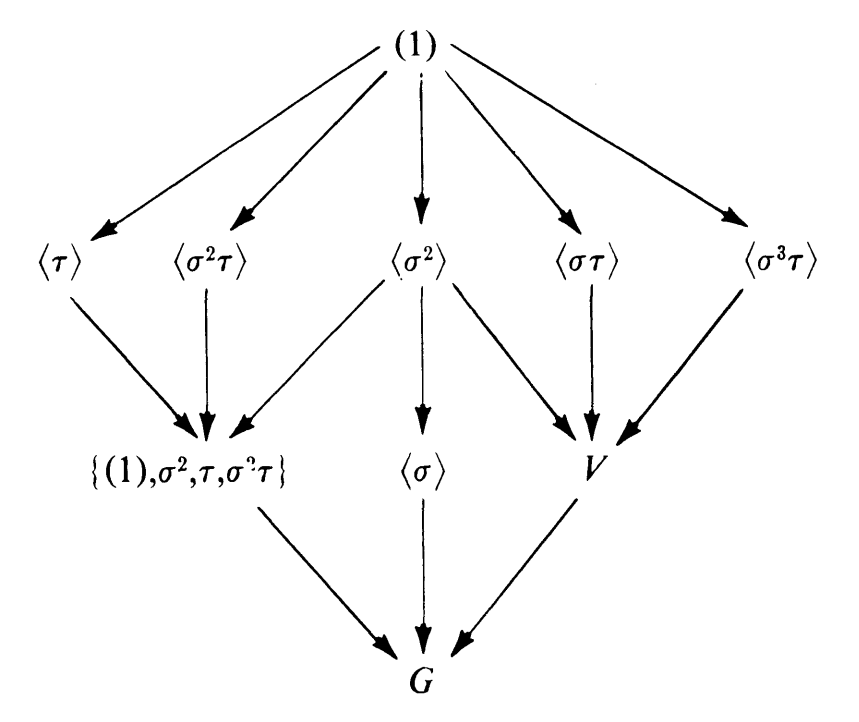
\includegraphics[scale=0.29]{Images/Subgroups.png}
    \caption{Subgroup lattice, where $H\to K$ means $H<K$}
\end{figure}
\begin{figure}[htbp]
    \center
    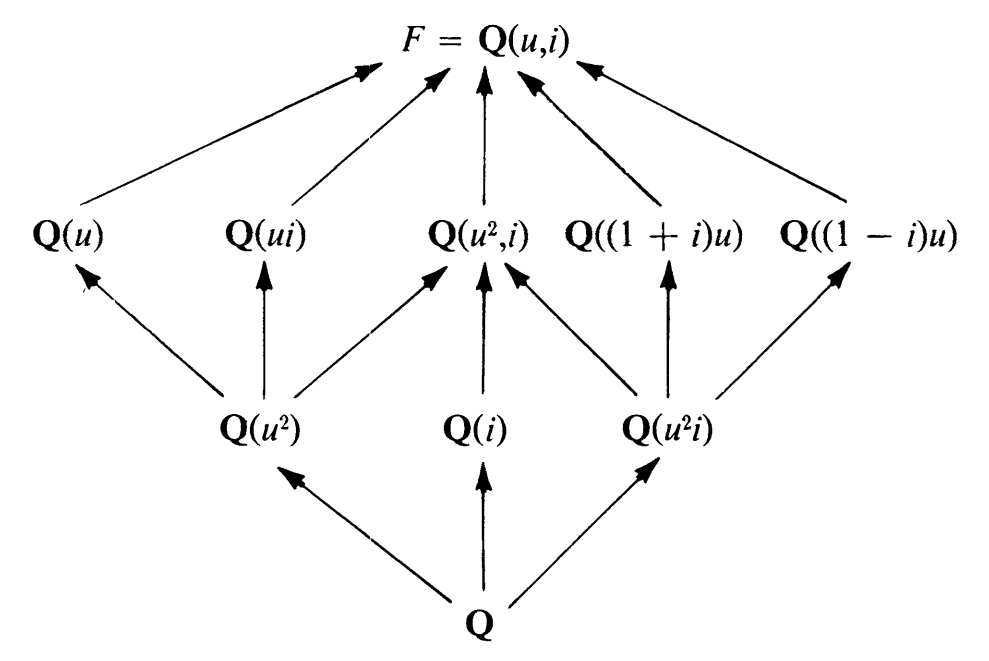
\includegraphics[scale=0.29]{Images/Intermediate Fields.png}
    \caption{Intermediate field lattice, where $M\to N$ means $M\subset N$}
\end{figure}
\end{example}
Specific techniques for computing Galois groups of polynomials of degree greater than $4$ are rather scarce. We shall we content with a very special case.
\begin{theorem}
If $p$ is prime and $f$ is an irreducible polynomial of degree $p$ over the field of rational numbers which has precisely two non-real roots in the field of complex numbers, then the Galois group of $f$ is (isomorphic to) $S_p$.
\end{theorem}
\begin{proof}
Let $G$ be the Galois group of $f$, then $p\mid |G|$. Therefore by Cauchy's theorem there exists some $\sigma\in G$ such that $\sigma$ is of order $p$. Since $\sigma\in S_n$, $\sigma$ is a $p$-cycle. Now complex conjugation is an $\mathbb{R}$-automorphism of $\mathbb{C}$ that moves every non-real elements. Therefore it interchanges the two non-real roots of $f$ and fix all others. This implies $G$ contains a transportation $\tau=(ab)$. We may suppose, by changing notation if necessary, that $\tau=(12)$ and $\sigma^k=(12\cdots p)$ for some $k$. However $\tau$ and $\sigma$ together generate $S_p$, hence $G=S_p$.
\end{proof}
\begin{center}
\begin{large}
    \textbf{Exercises for 6.4}
\end{large}
\end{center}
Unless stated otherwise $K$ is a field, $f\in K[x]$ and $F$ is a splitting field of $f$ over $K$.
\begin{problem}\em
Suppose $f\in K[x]$ splits in $F$ as $f=(x-u_1)^{n_1}\cdots (x-u_k)^{n_k}$ ($u_i$ distinct; $n_i\geq 1$). Let $v_0, ..., v_k$ be the coefficients of the polynomial $g=(x-u_1)(x-u_2)\cdots (x-u_k)$ and let $E=K(v_0, ..., v_k)$. Then \par
(i) $F$ is a splitting field of $g$ over $E$.\par
(ii) $F$ is Galois over $E$.\par
(iii) $\mathrm{Gal}(F/E)=\mathrm{Gal}(F/K)$.
\end{problem}
\begin{proof}
(i) Since $f$ splits in $F$ and $f$ and $g$ has the same roots (without counting the multiples), we have $g$ splits in $F$ and hence $F$ is a splitting field of $g$ over $E$.\par
(ii) Let $h\in E[x]$ be a polynomial in $E[x]$ that has a root in $F$. Then since $F$ is the splitting field over $E$, we have $h$ splits in $F$ and hence  $F/E$ is normal. By the definition of $E$ we have $h$ separable and hence $F/E$ is Galois.\par
(iii) Suppose $\sigma\in\mathrm{Aut}(F/K)$. Then $\sigma$ is a permutation of $\{u_1,\cdots,u_n\}$, where $u_i$ are the roots of a polynomial $g\in E[x]$. Therefore $\sigma$ actually fix $g$ and hence fix $E$. This implies $\sigma\in\mathrm{Gal}(F/E)$.
\end{proof}
\begin{problem}\em
Suppose $K$ is a subfield of $\mathbb{R}$ (so that $F$ may be taken to be a subfield of $\mathbb{C}$) and that $f$ is irreducible of degree $3$. Let $D$ be the discriminant of $f$. Then \par
(i) $D>0$ if and only if $f$ has three real roots.\par
(ii) $D<0$ if and only if $f$ has precisely one real root.
\end{problem}
\begin{proof}
We first show that if $\Delta^2>0$, then $\Delta\in\mathbb{R}$. Suppose $\Delta=a+b\mathrm{i}$, then $\Delta^2=a^2-b^2+2ab\mathrm{i}$. If $\Delta^2\in\mathbb{R}$, then $ab=0$. If $a=0$, then $\Delta^2=-b^2\le 0$, a contradiction! Therefore $\Delta=a\in\mathbb{R}$.\par
(i) Since $D=\Delta^2>0$, we have $\Delta\in\mathbb{R}$. Hence $\prod(u_i-u_j)\in\mathbb{R}$, which implies $u_i\in\mathbb{R}$.\par
(ii) Since $D=\Delta^2<0$, we have $\Delta\in\mathbb{C}-\mathbb{R}$. Hence $\prod(u_i-u_j)\in\mathbb{C}-\mathbb{R}$, which implies there exists at least one $u_i$ such that $u_i\in\mathbb{C}-\mathbb{R}$. However if there is only one such $u_i$, the square of $\Delta$ is either in $\mathbb{C}-\mathbb{R}$ or positive. Therefore there are two roots in $\mathbb{C}-\mathbb{R}$.
\end{proof}
\begin{problem}\em
Let $f$ be a separable cubic with Galois group $S_3$ and roots $u_1, u_2, u_3\in F$. Then the distinct intermediate fields of the extension of $K$ by $F$ are $F, K(\Delta), K(u_1), K(u_2), K(u_3), K$. The corresponding subgroups of the Galois group are $1, A_3, T_1, T_2, T_3$ and $S_3$ where $T_i=\{(1), (jk)\mid j\neq i\neq k\}$.
\end{problem}
\begin{proof}
Since the Galois group of $f$ is $S_3$, we have $\Delta\notin K$. Therefore we have the following Galois correspondence 
\begin{center}


\tikzset{every picture/.style={line width=0.75pt}} %set default line width to 0.75pt        

\begin{tikzpicture}[x=0.75pt,y=0.75pt,yscale=-1,xscale=1]
%uncomment if require: \path (0,476); %set diagram left start at 0, and has height of 476

%Straight Lines [id:da032329933164278346] 
\draw    (272,112) -- (272,158) ;
\draw [shift={(272,160)}, rotate = 270] [color={rgb, 255:red, 0; green, 0; blue, 0 }  ][line width=0.75]    (10.93,-3.29) .. controls (6.95,-1.4) and (3.31,-0.3) .. (0,0) .. controls (3.31,0.3) and (6.95,1.4) .. (10.93,3.29)   ;
%Straight Lines [id:da9414101801961103] 
\draw    (256,184) -- (201.74,215.01) ;
\draw [shift={(200,216)}, rotate = 330.26] [color={rgb, 255:red, 0; green, 0; blue, 0 }  ][line width=0.75]    (10.93,-3.29) .. controls (6.95,-1.4) and (3.31,-0.3) .. (0,0) .. controls (3.31,0.3) and (6.95,1.4) .. (10.93,3.29)   ;
%Straight Lines [id:da03991259947222936] 
\draw    (272,184) -- (272,214) ;
\draw [shift={(272,216)}, rotate = 270] [color={rgb, 255:red, 0; green, 0; blue, 0 }  ][line width=0.75]    (10.93,-3.29) .. controls (6.95,-1.4) and (3.31,-0.3) .. (0,0) .. controls (3.31,0.3) and (6.95,1.4) .. (10.93,3.29)   ;
%Straight Lines [id:da21039231506414402] 
\draw    (288,184) -- (342.26,215.01) ;
\draw [shift={(344,216)}, rotate = 209.74] [color={rgb, 255:red, 0; green, 0; blue, 0 }  ][line width=0.75]    (10.93,-3.29) .. controls (6.95,-1.4) and (3.31,-0.3) .. (0,0) .. controls (3.31,0.3) and (6.95,1.4) .. (10.93,3.29)   ;
%Straight Lines [id:da08651726223892764] 
\draw    (200,240) -- (262.3,278.94) ;
\draw [shift={(264,280)}, rotate = 212.01] [color={rgb, 255:red, 0; green, 0; blue, 0 }  ][line width=0.75]    (10.93,-3.29) .. controls (6.95,-1.4) and (3.31,-0.3) .. (0,0) .. controls (3.31,0.3) and (6.95,1.4) .. (10.93,3.29)   ;
%Straight Lines [id:da4999449076953608] 
\draw    (272,240) -- (272,278) ;
\draw [shift={(272,280)}, rotate = 270] [color={rgb, 255:red, 0; green, 0; blue, 0 }  ][line width=0.75]    (10.93,-3.29) .. controls (6.95,-1.4) and (3.31,-0.3) .. (0,0) .. controls (3.31,0.3) and (6.95,1.4) .. (10.93,3.29)   ;
%Straight Lines [id:da30117976366070653] 
\draw    (344,240) -- (281.7,278.94) ;
\draw [shift={(280,280)}, rotate = 327.99] [color={rgb, 255:red, 0; green, 0; blue, 0 }  ][line width=0.75]    (10.93,-3.29) .. controls (6.95,-1.4) and (3.31,-0.3) .. (0,0) .. controls (3.31,0.3) and (6.95,1.4) .. (10.93,3.29)   ;

% Text Node
\draw (267,95.4) node [anchor=north west][inner sep=0.75pt]    {$F$};
% Text Node
\draw (257,161.4) node [anchor=north west][inner sep=0.75pt]    {$K( \Delta )$};
% Text Node
\draw (177,220.4) node [anchor=north west][inner sep=0.75pt]    {$K( u_{1})$};
% Text Node
\draw (254,220.4) node [anchor=north west][inner sep=0.75pt]    {$K( u_{2})$};
% Text Node
\draw (329,220.4) node [anchor=north west][inner sep=0.75pt]    {$K( u_{3})$};
% Text Node
\draw (266,283.4) node [anchor=north west][inner sep=0.75pt]    {$K$};


\end{tikzpicture}
\end{center}
and the subgroups 
\begin{center}


\tikzset{every picture/.style={line width=0.75pt}} %set default line width to 0.75pt        

\begin{tikzpicture}[x=0.75pt,y=0.75pt,yscale=-1,xscale=1]
%uncomment if require: \path (0,476); %set diagram left start at 0, and has height of 476

%Straight Lines [id:da9414101801961103] 
\draw    (264,176) -- (201.7,214.94) ;
\draw [shift={(200,216)}, rotate = 327.99] [color={rgb, 255:red, 0; green, 0; blue, 0 }  ][line width=0.75]    (10.93,-3.29) .. controls (6.95,-1.4) and (3.31,-0.3) .. (0,0) .. controls (3.31,0.3) and (6.95,1.4) .. (10.93,3.29)   ;
%Straight Lines [id:da03991259947222936] 
\draw    (272,176) -- (272,214) ;
\draw [shift={(272,216)}, rotate = 270] [color={rgb, 255:red, 0; green, 0; blue, 0 }  ][line width=0.75]    (10.93,-3.29) .. controls (6.95,-1.4) and (3.31,-0.3) .. (0,0) .. controls (3.31,0.3) and (6.95,1.4) .. (10.93,3.29)   ;
%Straight Lines [id:da21039231506414402] 
\draw    (280,176) -- (342.3,214.94) ;
\draw [shift={(344,216)}, rotate = 212.01] [color={rgb, 255:red, 0; green, 0; blue, 0 }  ][line width=0.75]    (10.93,-3.29) .. controls (6.95,-1.4) and (3.31,-0.3) .. (0,0) .. controls (3.31,0.3) and (6.95,1.4) .. (10.93,3.29)   ;
%Straight Lines [id:da08651726223892764] 
\draw    (200,240) -- (262.3,278.94) ;
\draw [shift={(264,280)}, rotate = 212.01] [color={rgb, 255:red, 0; green, 0; blue, 0 }  ][line width=0.75]    (10.93,-3.29) .. controls (6.95,-1.4) and (3.31,-0.3) .. (0,0) .. controls (3.31,0.3) and (6.95,1.4) .. (10.93,3.29)   ;
%Straight Lines [id:da4999449076953608] 
\draw    (272,240) -- (272,278) ;
\draw [shift={(272,280)}, rotate = 270] [color={rgb, 255:red, 0; green, 0; blue, 0 }  ][line width=0.75]    (10.93,-3.29) .. controls (6.95,-1.4) and (3.31,-0.3) .. (0,0) .. controls (3.31,0.3) and (6.95,1.4) .. (10.93,3.29)   ;
%Straight Lines [id:da30117976366070653] 
\draw    (344,240) -- (281.7,278.94) ;
\draw [shift={(280,280)}, rotate = 327.99] [color={rgb, 255:red, 0; green, 0; blue, 0 }  ][line width=0.75]    (10.93,-3.29) .. controls (6.95,-1.4) and (3.31,-0.3) .. (0,0) .. controls (3.31,0.3) and (6.95,1.4) .. (10.93,3.29)   ;
%Straight Lines [id:da6118594202844929] 
\draw    (272,304) -- (272,342) ;
\draw [shift={(272,344)}, rotate = 270] [color={rgb, 255:red, 0; green, 0; blue, 0 }  ][line width=0.75]    (10.93,-3.29) .. controls (6.95,-1.4) and (3.31,-0.3) .. (0,0) .. controls (3.31,0.3) and (6.95,1.4) .. (10.93,3.29)   ;

% Text Node
\draw (262,158.4) node [anchor=north west][inner sep=0.75pt]    {$\left<1\right>$};
% Text Node
\draw (188,220.4) node [anchor=north west][inner sep=0.75pt]    {$T_{1}$};
% Text Node
\draw (262,220.4) node [anchor=north west][inner sep=0.75pt]    {$T_{2}$};
% Text Node
\draw (337,220.4) node [anchor=north west][inner sep=0.75pt]    {$T_{3}$};
% Text Node
\draw (261,284.4) node [anchor=north west][inner sep=0.75pt]    {$A_{3}$};
% Text Node
\draw (263,347.4) node [anchor=north west][inner sep=0.75pt]    {$S_{3}$};


\end{tikzpicture}
\end{center}
\end{proof}
\begin{problem}\em
If $\mathrm{char }K\neq 2, 3$ then the discriminant of $x^3+bx^2+cx+d$ is $-4c^3-27d^2+b^2(c^2-4bd)+18bcd$.
\end{problem}
\begin{proof}
This follows from a direct computation. Note that $\mathrm{char}K\ne 2,3$, hence the coefficients in the discriminant is valid.
\end{proof}
\begin{problem}\em
If $\mathrm{char }K\neq 2$ and $f\in K[x]$ is a cubic whose discriminant is a square in $K$, then $f$ is either irreducible or factors completely in $K$.
\end{problem}
\begin{proof}
Suppose $f$ is reducible in $K[x]$. Then there exists some $u\in K$ such that $u$ is a root of $f$. Note that the discriminant of $f$ is a square of $K$, therefore the Galois group of $f$ is $S_4$, hence there exists some permutations $\sigma$ such that $\sigma^k(u)$ consists of all root of $f$ when $k$ run over integers. Therefore $f$ splits in $K$ and hence factors completely in $K$.
\end{proof}
\begin{problem}\em
Over any base field $K$, $x^3-3x+1$ is either irreducible or splits over $K$.
\end{problem}
\begin{proof}
We compute the discriminant of the polynomial as follows: 
$$
D=\Delta ^2=-4\left( -3 \right) ^3-27=81=9^2,
$$
and since $\mathbb{Q}$ is the smallest number field we have $\mathbb{Q}\subset K$, hence $\Delta\in K$. Therefore by Exercise 6.51 we have $x^3-3x+1$ is either irreducible or splits over $K$.
\end{proof}
\begin{problem}\em
$S_4$ has no transitive subgroup of order $6$.
\end{problem}
\begin{proof}
We characterize the subgroups of order $6$ of $S_4$. Since the group of order $6$ must contain s Sylow $3$-subgroup, it is generated by a $3$-cycle and a $2$-cycle. Therefore all subgroups of $S_4$ of order $6$ is of the form $\{(ij)(ijk)\}$, where $\{i,j,k\}\subset\{1,2,3,4\}$. No such subgroups are transitive.
\end{proof}
\begin{problem}\em
Let $f$ be an (irreducible) separable quartic over $K$ and $u$ a root of $f$. There is no field properly between $K$ and $K(u)$ if and only if the Galois group of $f$ is either $A_4$ or $S_4$.
\end{problem}
\begin{proof}
Note that $[K(u):K]=4$. If there is a proper intermediate field $E$, then $[K(u):E]=[E:K]=2$. Therefore we have the following correspondence: 
$$
\begin{matrix}
	K&		\mapsto&		G\\
	\cap&		&		\land\\
	E&		\mapsto&		H\\
	\cap&		&		\land\\
	K\left( u \right)&		\mapsto&		L\\
	\cap&		&		\land\\
	K&		\mapsto&		1\\
\end{matrix}
$$
If $m=1$, then $G\cong V\cong\mathbb{Z}_2\oplus\mathbb{Z}_2$. Take $H=\mathbb{Z}_2\oplus\{0\}$ and $L=\{0\}$.\par
If $m=2$, then $G\cong D_4$ or $G\cong\mathbb{Z}_4$. If $G\cong D_4$, then take $H=\left<(ij)\right>$ and $L=\{0\}$. Otherwise take $H=\mathbb{Z}_2$ and $L=\{0\}$.\par
If $m=3$, then $G\cong A_4$. However there are no subgroups of $A_4$ of order $2$.\par
If $m=6$, then $G\cong S_4$. Then the only possible $H$ is $A_4$, however $A_4$ has no subgroups of order $2$.\par
Therefore if there exists some such intermediate fields, we have $m=1$ or $m=2$. Therefore there are no field properly between $K$ and $K(u)$ if and only if $m=3$ or $m=6$, i.e. the Galois group of $f$ is either $A_4$ or $S_4$.
\end{proof}
\begin{problem}\em
Let $x^4+ax^2+b\in K[x]$ (with $\mathrm{char }K\neq 2$) be irreducible with Galois group $G$.\par
(i) If $b$ is a square in $K$, then $G=V$.\par
(ii) If $b$ is not a square in $K$ and $b(a^2-4b)$ is a square in $K$, then $G\cong \mathbb{Z}_4$.\par
(iii) If neither $b$ nor $b(a^2-4b)$ is a square in $K$, then $G\cong D_4$.
\end{problem}
\begin{proof}
Note that the resolvant cubic of the polynomial $x^4+ax^2+b$ is $x^3-ax^2-4bx+4ab=(x-a)(x+2\sqrt{b})(x-2\sqrt{b})$. \par
(i) If $b$ is a square in $K$, then $m=1$, hence $G=V$.\par
(ii) If $b$ is not a square in $K$, note that $K(\alpha,\beta,\gamma)=K(\sqrt{b})$, we have $m=2$. Also note that 
$$
\begin{aligned}
x^4+ax^2+b&=\left( x^2-\frac{-a+\sqrt{a^2-4b}}{2} \right) \left( x^2-\frac{-a-\sqrt{a^2-4b}}{2} \right) 
\\
&=\left( x+\sqrt{\frac{-a+\sqrt{a^2-4b}}{2}} \right) \left( x-\sqrt{\frac{-a+\sqrt{a^2-4b}}{2}} \right) \left( x+\sqrt{\frac{-a-\sqrt{a^2-4b}}{2}} \right) \left( x-\frac{-a-\sqrt{a^2-4b}}{2} \right) ,
\end{aligned}
$$
it suffices to show that the four root actually lie in $K(\sqrt{b})$. Since $b(a^2-4b)$ is a square in $K$, we may suppose $\sqrt{a^2-4b}=t\sqrt{b}$ for some $t\in K$. Therefore 
$$
\sqrt{\frac{-a+\sqrt{a^2-4b}}{2}}=\sqrt{-\frac{a}{2}+\frac{t}{2}\sqrt{b}}=m+n\sqrt{b}
$$
for some $m,n\in K$, hence $x^4+ax^2+b$ is factored in $K(\sqrt{b})$, therefore $G=\mathbb{Z}_4$.\par
(iii) If $b(a^2-4b)$ is not a square in $K$, then $x^4+ax^2+b$ can't be factored in $K(\sqrt{b})$ and hence $G\cong D_4$.
\end{proof}
\begin{problem}\em
Determine all the subgroups of the Galois group and all of the intermediate fields of the splitting field (over $\mathbb{Q}$) of the polynomial $x^4-5\in \mathbb{Q}[x]$.
\end{problem}
\begin{proof}
Trivially the splitting field over $\mathbb{Q}$ of the polynomial $x^4-5$ is $\mathbb{Q}(\mathrm{i},\sqrt[4]{5})$. Let $\tau$ be the complex conjugation and $\sigma$ the rotation given by $z\mapsto\mathrm{i}z$, then we have the following diagram of intermediate fields 
$$
\begin{matrix}
	&		&		&		&		\mathbb{Q} (\mathrm{i},\sqrt[4]{5})&		&		\\
	&		&		&		\swarrow&		\downarrow&		\searrow&		\\
	&		&		\mathbb{Q} (\mathrm{i},\sqrt{5})&		&		\mathbb{Q} (\sqrt[4]{5})&		&		\mathbb{Q} (\mathrm{i}\sqrt[4]{5})\\
	&		\swarrow&		\downarrow&		\searrow&		\downarrow&		\swarrow&		\\
	\mathbb{Q} (\mathrm{i)}&		&		\mathbb{Q} (\mathrm{i}\sqrt{5})&		&		\mathbb{Q} (\sqrt{5})&		&		\\
	&		\searrow&		\downarrow&		\swarrow&		&		&		\\
	&		&		\mathbb{Q}&		&		&		&		\\
\end{matrix}
$$
and subgroups 
$$
\begin{matrix}
	&		&		&		&		\{1\}&		&		\\
	&		&		&		\swarrow&		\downarrow&		\searrow&		\\
	&		&		\langle \sigma ^2\rangle&		&		\langle \tau \rangle&		&		\langle \tau \sigma ^2\rangle\\
	&		\swarrow&		\downarrow&		\searrow&		\downarrow&		\swarrow&		\\
	\langle \sigma \rangle \cong \mathbb{Z} _4&		&		\langle \tau \sigma ,\sigma ^2\rangle \cong V&		&		\langle \tau ,\sigma ^2\rangle \cong V&		&		\\
	&		\searrow&		\downarrow&		\swarrow&		&		&		\\
	&		&		\langle \tau ,\sigma \rangle \cong D_4&		&		&		&		\\
\end{matrix}
$$
\end{proof}
\begin{problem}\em
Let $K$ be a subfield of the real numbers and $f\in K[x]$ an irreducible quartic. If $f$ has exactly two real roots, the Galois group of $f$ is $S_4$ or $D_4$.
\end{problem}
\begin{proof}
Since the polynomial has two real roots, the complex conjugation $\sigma$ lies in the Galois group of $f$. Note that $f$ is irreducible, the Galois group of $f$ is transitive. Hence the only candidates are $S_4$, $A_4$, $D_4$, $\mathbb{Z}_4$ and $\mathbb{Z}_2\oplus\mathbb{Z}_2$. However $\sigma$ is an odd permutation, therefore $\sigma\notin A_4$, so not in the subgroup $\mathbb{Z}_4$ of $A_4$. For $\mathbb{Z}_2\oplus\mathbb{Z}_2$, note that $\mathbb{Z}_2\oplus\mathbb{Z}_2=\{e,(12)(34),(13)(24),(14)(23)\}$, which does not contain a transposition.
\end{proof}
\subsection{Finite Fields}
In this section finite fields (sometimes called \textbf{Galois fields}) are characterized in terms of splitting fields and their structure completely determined. We begin with two theorems and a lemma that apply to fields which need not be finite. In each case, of course, we are interested primarily in the implications for finite fields.
\begin{theorem}
Let $F$ be a field and let $P$ be the intersection of all subfields of $F$. Then $P$ is a field with no proper subfields. If $\mathrm{char}F=p$ is a prime, then $P\cong\mathbb{Z}_p$. If $\mathrm{char}F=0$, then $P\cong\mathbb{Q}$, the field of rational numbers.
\end{theorem}
\begin{note}\em
The field $P$ is called the \textbf{prime subfield} of $F$.
\end{note}
\begin{proof}
We first show that $P$ is a subfield of $F$. Since $0$ and $1_F$ must lie in $P$, $P$ is nonempty. Suppose $x,y\in P$, then $x,y\in E$ for all $E$ a subfield of $F$. Therefore $x-y\in E$ and $x^{-1}y\in E$ for all $E\subset F$, hence $P=\bigcap E$ is also a field. Now if $E$ is a subfield of $F$, then by definition of $P$ we have $E\cap P=E$, hence $E=P$ and $P$ is the smallest subfield of $F$.\par
Now suppose $\mathrm{char}F=p$. Consider the map $\varphi:\mathbb{Z}\to P$ given by $m\mapsto m1_F$, then $\mathrm{Ker}\varphi=(p)$ and hence $\mathrm{Im}\varphi\cong\mathbb{Z}/(p)=\mathbb{Z}_p$. Since $\mathrm{Im}\varphi$ is a subfield of $P$, we have $\mathrm{Im}\varphi=P$ and hence $P\cong\mathbb{Z}_p$. Similarly we may prove $P\cong\mathbb{Q}$ when $\mathrm{char}F=0$.
\end{proof}
\begin{corollary}
If $F$ is a finite field, then $\mathrm{char}F=p\ne 0$ for some prime $p$, and $|F|=p^n$ for some integer $n\ge 1$.
\end{corollary}
\begin{proof}
Since $F$ is finite, the prime subfield of $F$ is finite and hence not isomorphic to $\mathbb{Q}$. Therefore $\mathrm{char}F\ne 0$. Since $F$ is a field, we therefore conclude that $\mathrm{char}F=p$ for some prime $p$. Now since $F$ is a finite dimensional vector space over $\mathbb{Z}_p$, we have $F\cong\mathbb{Z}_p\oplus\cdots\oplus\mathbb{Z}_p$ and hence $|F|=p^n$ for some $n\ge 1$.
\end{proof}
In the sequel we shall always identity the prime subfield of a field as $\mathbb{Z}_p$ or $\mathbb{Q}$ under the isomorphism given in Theorem 6.52. For instance, we shall write $\mathbb{Z}_p\subset F$, and $1_F=1\in\mathbb{Z}_p$.
\begin{theorem}
If $F$ is a field and $G$ is a finite subgroup of the multiplicative group of nonzero elements of $F$, then $G$ is a cyclic group. In particular, the multiplicative group of all nonzero elements of finite fields is cyclic.
\end{theorem}
\begin{proof}
Suppose $G\cong\mathbb{Z}_{m_1}\oplus\mathbb{Z}_{m_2}\oplus\cdots\oplus\mathbb{Z}_{m_k}$ and $m_1\mid m_2\mid\cdots\mid m_k$, or otherwise the condition is trivial. Therefore $m_k\left(\bigoplus_{i=1}^k\mathbb{Z}_{m_i}\right)=0$, it follows that every $u\in G$ is a root of $x^{m_k}-1_F\in F[x]$. Note that the polynomial has at most $m_k$ distinct roots in $F$, we have $G\cong\mathbb{Z}_{m_k}$.
\end{proof}
\begin{corollary}
If $F$ is a finite field, then $F$ is a simple extension of its prime subfield $\mathbb{Z}_p$, that is, $F=\mathbb{Z}_p(u)$ for some $u\in F$.
\end{corollary}
\begin{proof}
Let $u$ be the generator of the multiplicative group of nonzero elements of $F$.
\end{proof}
\begin{lemma}\em
If $F$ is a field of characteristic $p$ and $r\ge 1$ is an integer, then the map $\varphi:F\to F$ given by $u\mapsto u^{p^r}$ is a $\mathbb{Z}_p$-monomorphism of fields. If $F$ is finite, then $\varphi$ is a $\mathbb{Z}_p$-automorphism of $F$.
\end{lemma}
\begin{proof}
Note that in the field of characteristic $p$ we have $(u+v)^p=u^p+v^p$, therefore if $u^{p^r}=v^{p^r}$, we have $u^{p^r}-v^{p^r}=(u-v)^{p^r}=0$, hence $u-v=0$ and $u=v$. Therefore $\varphi$ is a monomorphism. Now if $k\in\mathbb{Z}_p$, we have $k^{p^r}=k$ and hence $\varphi$ fix $\mathbb{Z}_p$.
\end{proof}
We can now give a useful characterization of finite fields.
\begin{proposition}
Let $p$ be a prime and $n\ge 1$ an integer. Then $F$ is a finite field with $p^n$ elements if and only if $F$ is a splitting field of $x^{p^n}-x$ over $\mathbb{Z}_p$.
\end{proposition}
\begin{proof}
If $|F|=p^n$, then the multiplicative group of nonzero elements of $F$ has order $p^n-1$ and hence every nonzero element $u\in F$ satisfies $u^{p^n-1}=1_F$. Therefore $u$ is a root of $x^{p^n-1}-1_F$ and therefore a root of $x(x^{p^n-1}-1_F)=x^{p^n}-x$. Since $0\in F$ is also a root of $x^{p^n}-x$, we have $x^{p^n}-x$ splits in $F$ and hence $F$ is a splitting field over $\mathbb{Z}_p$ of the polynomial $x^{p^n}-x$.\par
Conversely, suppose $x^{p^n}-x$ splits in $F$. Note that $x^{p^n}-x$ has $p^n$ distinct elements in $F$. If $\varphi$ is the monomorphism as defined in Lemma 6.15, we have $u$ is a root of $x^{p^n}-x$ if and only if $\varphi(u)=u$. Let $E$ be the set of all $u\in F$ such that $\varphi(u)=u$. Therefore suppose $u$ and $v\in E$ , we have $(u+v)^{p^n}=u+v$, $(uv)^{p^n}=uv$ and $(u^{-1})^{p^n}=u^{-1}$, therefore the set of all such $u$ that $\varphi(u)=u$ is a field of order $p^n$, and hence $F=\mathbb{Z}_p(E)=E$.
\end{proof}
\begin{corollary}
If $p$ is a prime and $n\ge 1$ an integer, then there exists a field with $p^n$ elements. Any two finite fields with the same number of elements are isomorphic.
\end{corollary}
\begin{proof}
To show the existence, consider a splitting field over $\mathbb{Z}_p$ of the polynomial $x^{p^n}-x$. Note that any field of order $p^n$ is a splitting field over $\mathbb{Z}_p$ of the polynomial $x^{p^n}-x$, we have any two finite fields with the same number of elements are isomorphic.
\end{proof}
\begin{corollary}
If $K$ is a finite field and $n\ge 1$ is an integer, then there exists a simple extension field $F=K(u)$ of $K$ such that $F$ is finite and $[F:K]=n$. Any two $n$-dimensional extension fields of $K$ are $K$-isomorphic.
\end{corollary}
\begin{proof}
Given $K$ of order $p^r$. Let $F$ be a splitting field over $K$ of $f=x^{p^{nr}}-x$. Note that for all $u\in K$, we have $u^{p^r}=u$, hence by induction we have $u^{p^{rn}}=u$. Therefore $K$ is the field of $\mathbb{Z}_p$ adjoined with \textit{some} roots of $f$. Therefore by Exercise 6.31 we have $F/\mathbb{Z}_p$ is a splitting field of $f$. Hence $F$ consists of precisely the $p^{nr}$ roots of $f$. Therefore $p^{nr}=\left| F \right|=\left| K \right|^{\left[ F:K \right]}=\left( p^r \right) ^{\left[ F:K \right]}$, hence $[F:K]=n$. By Corollary 6.55 we know that $F$ is a simple extension of $K$.\par
Now if there is another extension field $F_1$ such that $[F_1:K]=n$, then $[F_1:\mathbb{Z}_p]=[F_1:K][K:\mathbb{Z}_p]=p^{nr}$, hence $F_1$ is a splitting field over $\mathbb{Z}_p$ of $f$ and hence $F_1\cong F$.
\end{proof}
\begin{corollary}
If $K$ is a finite field and $n\ge 1$ an integer, then there exists an irreducible polynomial of degree $n$ in $K[x]$.
\end{corollary}
\begin{proof}
If there were no such irreducible polynomials, then for all $u\in\overline{K}$ we have $[K(u):K]\ne n$. However by Corollary 6.28 there exists some $u$ such that $[K(u):K]=n$, a contradiction!
\end{proof}
\begin{proposition}
If $F$ is a finite dimensional extension field of a finite field $K$, then $F$ is finite and is Galois over $K$. The Galois group $\mathrm{Gal}(F/K)$ is cyclic.
\end{proposition}
\begin{proof}
Let $\mathbb{Z}_p$ be the prime subfield of $K$. Then $F$ is a finite dimensional over $\mathbb{Z}_p$. Suppose $[F:\mathbb{Z}_p]=n$, then $|F|=p^n$. By Proposition 6.56 $F$ is a splitting field over $\mathbb{Z}_p$ of the polynomial $x^{p^n}-x$, hence a splitting field over $K$. Since the zeros of the polynomial $x^{p^n}-x$ are distinct, we have $F/K$ is separable and hence $F/K$ a Galois extension. By Lemma 6.15 the map $\varphi:F\to F$ given by $u\mapsto u^p$ is a $\mathbb{Z}_p$-automorphism. Clearly $\varphi^n$ is the identity map and $n$ is the least positive integer $k$ such that $\varphi^k$ is an identity. Since $|\mathrm{Aut}(G/\mathbb{Z}_p)|=n$ by the Fundamental theorem, we have $|\mathrm{Aut}(G/\mathbb{Z}_p)|$ is generated by $\varphi$, which is cyclic. Note that the subgroup of a cyclic group is cyclic, we have $\mathrm{Gal}(F/K)$ cyclic.
\end{proof}
\begin{center}
\begin{large}
    \textbf{Exercises for 6.5}
\end{large}
\end{center}
$F$ always denotes an extension field of a field $K$.
\begin{problem}\em
If $K$ is a finite field of characteristic $p$, describe the structure of the additive group of $K$.
\end{problem}
\begin{proof}
Since $K$ is a finite field of characteristic $p$, we have $|K|=p^m$ for some $m=[K:\mathbb{Z}_p]$. Therefore $K$ may be seen as a $m$-dimensional vector space over $\mathbb{Z}_p$, hence we have $K\cong\mathbb{Z}_p\oplus\mathbb{Z}_p\oplus\cdots\oplus\mathbb{Z}_p$ ($m$ summonds). Therefore we obtain the structure of the additive group $(K,+)=(\mathbb{Z}_p^m,+)$.
\end{proof}
\begin{problem}\em
(Fermat) If $p\in \mathbb{Z}$ is prime, then $a^p=a$ for all $a\in \mathbb{Z}_p$ or equivalently, $c^p\equiv c\pmod{p}$ for all $c\in \mathbb{Z}$.
\end{problem}
\begin{proof}
Consider $\mathbb{Z}_p$ as the splitting field of the polynomial $x^p-x$. Therefore we have for all $a\in\mathbb{Z}_p$ we have $a^p-a=0$. Therefore $a^p=a$ in $\mathbb{Z}_p$ and $c^p\equiv c(\mathrm{mod}\ p)$ for all $c\in\mathbb{Z}$.
\end{proof}
\begin{problem}\em
If $|K|=p^n$, then every element of $K$ has a unique $p$th root in $K$.
\end{problem}
\begin{proof}
Suppose $\alpha\in K$. We consider the polynomial $x^p-\alpha$. Since the derivative of $x^p-\alpha$ is zero, it has multiple roots. Indeed suppose $\beta$ is a root of $x^p-\alpha$, we have $(x-\beta)^p=x^p-\beta^p=x^p-\alpha$, hence $\beta$ is the only root of $x^p-\alpha$ without counting multiples. Now we show that $\beta\in K$. Consider the mapping $\alpha\mapsto\alpha^p$, by Lemma 6.15 and the fact that $K$ is a finite field we have the mapping is an automorphism, hence $\alpha^p\in K$.
\end{proof}
\begin{problem}\em
If the roots of a monic polynomial $f\in K[x]$ (in some splitting field of $f$ over $K$) are distinct and form a field, then $\mathrm{char}K=p$ and $f=x^{p^n}-x$ for some $n\geq 1$.
\end{problem}
\begin{proof}
Suppose $F$ is a splitting field over $K$ of $f$. Then $F\supset E\supset K$, where $E$ is the set of all root of $f$. Now since $F/E$ is a splitting field over $E$, we have $F=E$. Since $E$ is a finite field, we may suppose $|E|=p^n$ for some prime $p$ and $n\in\mathbb{N}$. Therefore $|E|=|K|^{[E:K]}$ implies $|K|=p$ and $[E:K]=n$. This gives $\mathrm{char}K=p$, $K=\mathbb{Z}_p$ and $f=x^{p^n}-x$, $n\ge 1$.
\end{proof}
\begin{problem}\em
Construct a field with $9$ elements and give its addition and multiplication tables.
\end{problem}
\begin{proof}
An example of a field with $9$ elements is $\mathbb{Z}_3\oplus\mathbb{Z}_3\oplus\mathbb{Z}_3$. We omit the addition and multiplication tables.
\end{proof}
\begin{problem}\em
If $|K|=q$ and $\gcd{(n, q)}=1$ and $F$ is a splitting field of $x^n-1_K$ over $K$, then $[F:K]$ is the least positive integer $k$ such that $n\mid (q^k-1)$.
\end{problem}
\begin{proof}
We first show that $n\mid(q^k-1)$. Since $F$ is a splitting field of the polynomial $x^n-1_K$ over $K$, we have $|F|=|K|^{[F:K]}=q^k$. Consider $F^\times=F-\{0\}$, then $|F^\times|=q^k-1$. Note that there exists some $u\in F^\times$ such that $u^n=1_K$, hence $u$ is an element of order $n$. Therefore by Cauchy's theorem we have $n\mid|F^\times|=q^k-1$.\par
To show that $k$ is the least element such that $n\mid(q^k-1)$, suppose there exists another $j<k$ satisfy $n\mid(q^j-1)$. Then there exists a finite field $E$ of order $q^j$ that contain an element $v$ of order $n$. Therefore $v$ is a root of $x^n-1_K$ and hence $E$ a splitting field of $x^n-1$ over $K$. However by the uniqueness of splitting fields, we have $j=k$, a contradiction!
\end{proof}
\begin{problem}\em
If $|K|=q$ and $f\in K[x]$ is irreducible, then $f$ divides $x^{q^n}-x$ if and only if $\deg{f}$ divides $n$.
\end{problem}
\begin{proof}
Suppose first $f\mid h$, where $h=x^{q^n}-x$. We suppose $\mathrm{deg}f=d$. Since $h$ splits in $\mathbb{Z}_{q^n}$, we have $f$ splits in $\mathbb{Z}_{q^n}$. Suppose $\alpha$ is a root of $f$, then $\alpha\in\mathbb{Z}_{q^n}$ and $\mathbb{Z}_q(\alpha):\mathbb{Z}_q]=d$. Therefore $n=[\mathbb{Z}_{q^n}:\mathbb{Z}_q]=[\mathbb{Z}_{q^n}:\mathbb{Z}_q(\alpha)][\mathbb{Z}_{q}(\alpha):\mathbb{Z}_q]=[\mathbb{Z}_{q^n}:\mathbb{Z}_q(\alpha)]d$, hence $d\mid n$. Conversely, suppose $d\mid n$. Say $n=pd$ for some $p$. We consider the quotient field (it is a field since $f$ is irreducible over $\mathbb{Z}_q$) $\mathbb{Z}_q[x]/(f)\cong\mathbb{Z}_{q^d}$, where the isomorphism follows from identifying $\mathbb{Z}_{p^d}$ as a simple extension of $\mathbb{Z}_p$ adjoining a root of $h$. Therefore suppose $x+(f)\in\mathbb{Z}_q[x]/(f)$, we have $(x+(f))^{q^n}=(x+(f))^{q^{pd}}=x+(f)$. Hence $x^{q^n}-x\in (f)$ and $f\mid h$.
\end{proof}
\begin{problem}\em
If $|K|=p^r$ and $|F|=p^n$, then $r\mid n$ and $\mathrm{Aut}_K F$ is cyclic with generator $\varphi$ given by $u\mapsto u^{p^r}$.
\end{problem}
\begin{proof}
Note that $[F:\mathbb{Z}_p]=n$ and $[K:\mathbb{Z}_p]=r$, we have $[F:K]=n/r\in\mathbb{Z}$, whence $r\mid n$. Now since any finite extension of finite fields are Galois, we have $|\mathrm{Gal}(F/K)|=[F:K]$ is a cyclic group as a subgroup of $\left<\phi\right>$, where $\phi:u\mapsto u^p$. Therefore $\mathrm{Gal}(F/K)=\left<\varphi\right>$ with $\varphi:u\mapsto u^{p^r}$.
\end{proof}
\begin{problem}\em
If $n\geq 3$, then $x^{2^n}+x+1$ is reducible over $\mathbb{Z}_2$.
\end{problem}
\begin{proof}
We observe that 
$$
\begin{aligned}
x^{2^n}+x+1&=\left( x^{2^n}+x^{2^{n-1}}+1 \right) +\left( x^{2^{n-1}}+x^{2^{n-2}}+1 \right) +\cdots +\left( x^2+x+1 \right) 
\\
&=\sum_{k=0}^{n-1}{\left( x^{2^{k+1}}+x^{2^k}+1 \right)}=\sum_{k=0}^{n-1}{\left( x^2+x+1 \right) ^{2^k}}
\\
&=\left( x^2+x+1 \right) \left( \sum_{k=0}^{n-1}{\left( x^2+x+1 \right) ^{2^k-1}} \right) ,
\end{aligned}
$$
therefore $x^2+x+1\mid x^{2^n}+x+1$ in $\mathbb{Z}_2$.
\end{proof}
\begin{problem}\em
Every element in a finite field may be written as the sum of two squares.
\end{problem}
Since any finite field has order $p^n$ with $p$ prime. Since $\mathbb{Z}_{p^n}\cong\mathbb{Z}\oplus\cdots\oplus\mathbb{Z}$ ($n$ summands), it suffices to prove for $\mathbb{Z}_p$. If $p=2$, trivial. We now prove the condition of $p\ge 3$.\par
Consider $S=\{x^2:x\in\mathbb{Z}_p\}$. For $k\in\mathbb{Z}_p$, we define $S(k)=\{k-x^2:x\in\mathbb{Z}_p\}$. Note that the map $x\mapsto x^2$ is a two-to-one endomorphism of $\mathbb{Z}_p^\times$ (since for all $x\in\mathbb{Z}_p$, we have $(p-x)^2=p^2-2px+x^2=x^2$ and hence the image of $x$ and $p-x$ coincide), we have $|S|=\frac{p+1}{2}$. Therefore there exists some $x^2\in S$ and $k-y^2\in S(k)$ such that $x^2=k-y^2$, which is $x^2+y^2=k$.
\subsection{Separability}
Our study of separability will be greatly facilitated by the simultaneous consideration of an concept that is, in a sense, the complete opposite of separability.
\begin{definition}
Let $F$ be an extension field of $K$. An algebraic element $u\in F$ is \textbf{purely inseparable} over $K$ if its irreducible polynomial $f$ in $K[x]$ factors in $F[x]$ as $f=(x-u)^m$. $F$ is a \textbf{purely inseparable extension} of $K$ if every element of $F$ is purely inseparable over $K$.
\end{definition}
Thus $u$ is separable over $K$ if its irreducible polynomial $f$ of degree $n$ has $n$ distinct roots in some splitting field of $K$, and purely inseparable over $K$ if $f$ has precisely one root. It is clearly possible that an element is either separable and purely inseparable over $K$.
\begin{theorem}
Let $F$ be an extension field of $K$. Then $u\in F$ is both separable and purely inseparable over $K$ if and only if $u\in K$.
\end{theorem}
\begin{proof}
Suppose $u\in F$ is both separable and purely inseparable. Then the irreducible polynomial of $u$ is of the form 
$$
f\left( x \right) =\prod_{i=1}^n{\left( x-u_i \right)}=\left( x-u \right) ^m.
$$
Therefore $f(x)=x-u$ and hence $u\in K$. Conversely, if $u\in K$, then the irreducible polynomial of $f=x-u\in K[x]$. Hence $u$ is both separable and purely inseparable.
\end{proof}
If $\mathrm{char}K=0$, then every irreducible polynomial over $K$ is separable. Therefore the only elements that are purely inseparable over $K$ are the elements of $K$ itself. Consequently we shall now consider the condition $\mathrm{char}K=p$. In order to characterize purely inseparable extensions we need 
\begin{lemma}\em
Let $F$ be an extension field of $K$ with $\mathrm{char}K=p\ne 0$. If $u\in F$ is separable over $K$, then $u^{p^n}$ is separable over $K$ for some $n\ge 0$.
\end{lemma}
\begin{proof}
We prove by induction. Suppose $u\in F$ is of degree one, then the conclusion follows trivially. Now suppose $\mathrm{deg}u=n>1$. Then the irreducible polynomial $f$ of $u$ has degree greater than one and $f^\prime(u)=0$, which implies that $f$ is a polynomial of $x^p$, whence we may regard $f$ as a polynomial of $x^p$ of degree less than $n$. Therefore by our induction hypothesis we have $(u^p)^{p^m}$ is separable over $K$ for some $m\ge 0$.
\end{proof}
\begin{theorem}
If $F$ is an algebraic extension field of a field $K$ of characteristic $p\ne 0$, then the following statements are equivalent:\par
(i) $F$ is purely inseparable over $K$;\par
(ii) The irreducible polynomial of any $u\in F$ is of the form $x^{p^n}-a\in K[x]$;\par
(iii) If $u\in F$, then $u^{p^n}\in K$ for some $n\ge 0$;\par
(iv) The only elements of $F$ which are separable over $K$ are the elements of $K$ itself;\par
(v) $F$ is generated over $K$ by a set of purely inseparable elements.
\end{theorem}
\begin{proof}
We first show that the first three statements are equivalent.\par
(i)$\Rightarrow$(ii): This is the most tricky part. The rest proof of this theorem is rather trivial. Suppose $u\in F$. Since $F$ is a purely inseparable extension field of $K$, we have the irreducible polynomial of $u$ is $f=(x-u)^m$. Suppose $m=np^r$, where $(n,p)=1$. Then $f=(x^{p^r}-u^{p^r})^n$. Since $f\in K[x]$, the coefficient of $x^{p^r(n-1)}$ lies in $K$, and hence $\pm nu^{p^r}\in K$. We claim that $u^{p^r}\in K$. Suppose $u^{p^r}=v$. Since $(p,n)=1$, by Bezout's theorem we have $kp+ln=1$ for some $k,l\in\mathbb{Z}$. Therefore $kpv+lnv=v$. Now $lnv\in K$ and $kpv=0$ since $\mathrm{char}K=p$, hence $v\in K$. Therefore $f=(x^{p^r}-v)^n$ and $u$ is purely inseparable, this is to say $n=1$ and hence $f=x^{p^r}-v$.\par
(ii)$\Rightarrow$(iii): Suppose $u\in F$, then the irreducible polynomial of $u$ is $x^{p^n}-a$ for some $a\in K$. Therefore $u^{p^n}\in K$ for some $n$.\par
(iii)$\Rightarrow$(i): Suppose $u\in F$, then there exists some $n\in\mathbb{Z}_+$ such that $u^{p^n}\in K$. Therefore $f=(x-u)^{p^n}$ has a root $u$. We may select the least $n$ such that $u^{p^n}\in K$, and hence such $f$ is irreducible and the irreducible polynomial of $f$. Therefore $u$ is purely inseparable over $K$.\par
(i)$\Rightarrow$(iv): Suppose $u\in F$. Then $u$ is purely inseparable over $K$. Now if $u$ is separable over $K$, we have $u$ being both purely inseparable and separable over $K$, hence $u\in K$.\par
(iv)$\Rightarrow$(iii): Suppose $u\in F$. By Lemma 6.16 we know that there exists some $n\ge 0$ such that $u^{p^n}$ is separable over $K$. However the only elements that are separable over $K$ are the elements of $K$ itself, hence $u^{p^n}\in K$.\par
(i)$\Rightarrow$(v): Let $X$ be the set of all purely inseparable elements in $F$ over $K$, then $F=K(X)$.\par
(v)$\Rightarrow$(iii): If $u$ is purely inseparable over $K$, then $u\in K(x_1,\cdots,x_m)$ for some $x_i$ purely inseparable over $K$, therefore $u=\sum k_ix_i$ and hence $u$ is also inseparable.
\end{proof}
\begin{corollary}
If $F$ is a finite dimensional purely inseparable extension field of $K$ and $\mathrm{char}K=p\ne 0$, then $[F:K]=p^n$ for some $n\ge 0$.
\end{corollary}
\begin{proof}
Suppose $F=K(u_1,\cdots,u_m)$, where each $u_i$ is purely inseparable over $K$. Then $u_i$ is purely inseparable over $K(u_1,\cdots,u_{i-1})$ by definition of purely inseparable elements. Therefore we may consider the tower of field extensions: 
$$
K\subset K\left( u_1 \right) \subset K\left( u_1,u_2 \right) \subset \cdots K\left( u_1,\cdots ,u_n \right) =F.
$$
Notice that by Lemma 6.16 we have each $[K(u_1,\cdots,u_i):K(u_1,\cdots,u_{i-1})]$ is a power of $p$, and hence $[F:K]=p^n$ for some $n\ge 0$.
\end{proof}
One more preliminary is needed for the principal theorem on separability.
\begin{lemma}\em
If $F$ is an extension field of $K$, $X$ is a subset of $F$ such that $F=K(X)$, and every element of $X$ is separable over $K$, then $F$ is a separable extension of $K$.
\end{lemma}
\begin{proof}
Suppose $v\in F$, then $v\in K(u_1,\cdots,u_n)$ for some $u_i\in X$. Suppose $f_i$ is the irreducible polynomial of $u_i$ in $K$, then by the definition of $X$ we have $f_i$ is separable over $K$. Now suppose $E$ is a splitting field over $K(u_1,\cdots,u_n)$ of $\{f_1,\cdots,f_n\}$. Then $E$ is also a splitting field over $K$ of $\{f_1,\cdots,f_n\}$. Therefore $E$ is Galois over $K$, and hence separable over $K$.
\end{proof}
\begin{theorem}
Let $F$ be an algebraic extension field of $K$, $S$ be the set of all elements of $F$ which are separable over $K$, and $P$ the set of all elements of $F$ which are purely inseparable over $K$.\par
(i) $S$ is a separable extension field of $K$.\par
(ii) $F$ is a purely inseparable over $S$.\par
(iii) $P$ is purely inseparable extension field of $K$.\par
(iv) $P\cap S=K$.\par
(v) $F$ is separable over $P$ if and only if $F=SP$.\par
(vi) If $F$ is normal over $K$, then $S$ is Galois over $K$, $F$ is Galois over $P$ and $\mathrm{Gal}(S/K)\cong\mathrm{Gal}(F/P)\cong\mathrm{Aut}(F/K)$.
\end{theorem}
\begin{proof}
(i) Clearly every element of $S$ is separable over $K$. It suffices to show that $S$ is a field. Indeed, suppose $u,v\in S$, then consider the field $K(u,v)$, by Lemma 6.17 we have it is a separable extension of $K$. Therefore $u-v\in S$ and $uv^{-1}\in S$ provided $v\ne 0$. This proved that $S$ is a field.\par
(ii) Suppose first that $\mathrm{char}K=0$. Then every element over $K$ is separable and hence $S=F$. Therefore the extension $F/S$ is trivial and hence purely inseparable. Now if $\mathrm{char}K=p$, for an arbitrarily chosen $u\in F$ we have $u^{p^n}$ is separable over $K$ for some $n\ge 0$. Therefore $u^{p^n}\in S$ for some $n\ge 0$ and hence $F/S$ is purely inseparable by Theorem 6.63.\par
(iii) The prove goes similar to (i) and we omit the details.\par
(iv) Suppose $u\in P\cap S$, then $u$ is purely inseparable and separable over $K$, therefore $u\in K$. Conversely, if $u\in K$, then $u\in P$ and $u\in S$, therefore $K=P\cap S$.\par
(v) Suppose $F$ is separable over $P$. Then $F$ is also separable over $SP$. However since $F$ is purely inseparable over $S$, we have $F$ purely inseparable over $SP$ and hence $F/SP$ is purely inseparable and separable. This could only happen when $F=SP$. Conversely, suppose $F=SP$, then $F=P(S)$. By Lemma 6.17 we have $F$ is separable over $P$.\par
(vi) We first show that the fix field of $\mathrm{Aut}(F/K)$ is $P$, which implies that $F/P$ is Galois and $\mathrm{Aut}(F/K)\cong\mathrm{Gal}(F/P)$. Now suppose the fixed field of $\mathrm{Aut}(F/K)=K_0$. Suppose first $u\in P$ and $\sigma\in\mathrm{Aut}(F/K)$. Then since $u$ is purely inseparable over $K$, we have $\sigma(u)=u$ since $\sigma$ is also a root of the irreducible polynomial of $u$. Therefore $u$ is fixed by $\sigma$ and hence $u\in K_0$. To prove the converse inclusion, suppose $u\in K_0$. Now suppose $v\in F$ is another root of the irreducible polynomial $f$ of $u$, we have an isomorphism $\tau:K(u)\to K(v)$ such that $\tau(u)=v$. Now since the extension $F/K$ is normal, we have $F$ a splitting field over $K$ of $f$, and hence there exists an extension of $\tau$ (we shall continue to denote the extension isomorphism as $\tau$) that is an automorphism of $F$. Therefore since $\tau(u)=v$, we have $u=\tau(u)=v$ and hence $f=(x-u)^m$ for some $m$. Therefore $u\in P$ and $P\supset K_0$. This implies $P=K_0$ and hence we have shown that $F/P$ is Galois and $\mathrm{Gal}(F/P)=\mathrm{Aut}(F/K)$.\par
To prove the rest part of the theorem, we note that every $\sigma\in\mathrm{Gal}(F/P)$ must send separable elements into separable elements. Therefore $\theta:\mathrm{Gal}(F/P)\to\mathrm{Aut}(S/K)$ given by $\sigma\mapsto\sigma\mid_S$ defines a homomorphism. It suffices to show that $\theta$ is an isomorphism. First note that $F/K$ is normal, therefore $F$ is a splitting field of $K$. Now for each $\sigma\in\mathrm{Aut}(S/K)$ we may extend $\sigma$ onto $F$ (denoted as $\widetilde{\sigma}$), and hence $\theta(\widetilde{\sigma})=\sigma$. Therefore $\theta$ is an epimorphism. Now since $F$ is Galois over $P$, we have $F/P$ is separable. Therefore by (v) we have $F=SP$ and hence $\theta$ is a monomorphism. This implies $\theta$ is indeed an isomorphism and hence $\mathrm{Gal}(F/P)\cong\mathrm{Aut}(S/K)$. Finally suppose $u\in S$ that is fixed by all $\sigma\in\mathrm{Aut}(S/K)$, we have $u$ is also in the fixed field $P$ of $\mathrm{Gal}(F/P)$ since $\theta$ is an epimorphism. Therefore $u\in S\cap P=K$ and hence $S/K$ is Galois. Combine the preceding discussion we conclude that $\mathrm{Gal}(F/P)\cong\mathrm{Gal}(S/K)\cong\mathrm{Aut}(F/K)$.
\end{proof}
\begin{corollary}
If $F$ is a separable extension field of $E$ and $E$ is a separable extension field of $K$, then $F$ is separable over $K$.
\end{corollary}
\begin{proof}
Let $S$ as defined in Theorem 6.65. Then $E\subset S$ and $F$ is purely inseparable over $S$. But $F$ is separable over $E$ and hence over $S$, hence $F=S$ and $F$ is separable over $K$.
\end{proof}
\begin{corollary}
Let $F$ be an algebraic extension field of $K$, with $\mathrm{char}K=p\ne 0$. If $F$ is separable over $K$, then $F=KF^{p^n}$ for each $n\ge 1$. If $[F:K]$ is finite and $F=KF^p$, then $F$ is separable over $K$. In particular, $u\in F$ is separable over $K$ if and only if $K(u^p)=K(u)$.
\end{corollary}
\begin{proof}
We first suppose $F$ is separable over $K$, then $F$ is separable over $KF^{p^n}$. However $F$ is purely inseparable over $KF^{p^n}$ by Theorem 6.63, hence the only possibility is that $F=KF^{p^n}$.\par
Now suppose $[F:K]$ is finite. Then there exists some $u_1,\cdots,u_m$ such that $F=K(u_1,\cdots,u_m)=S(u_1,\cdots,u_m)$. Since each $u_i$ is purely inseparable over $S$, there exists some $n\ge 0$ such that $u_i^{p^n}\in S$ for every $i$. Since $F=S(u_1,\cdots,u_m)$ we have $F^{p^n}\subset S$. Clearly every element of $S$ is purely inseparable over $F^{p^n}$, therefore $S$ is purely inseparable over $KF^{p^n}$. However by definition of $S$ we have $S$ is separable over $K$, hence $S$ is separable over $KF^{p^n}$, this implies $S=KF^{p^n}$. Now since $\mathrm{char}K=p$, we have that for any $t\ge 1$, 
$$
F^{p^t}=\left[ K\left( u_1,\cdots ,u_m \right) \right] ^{p^t}=K^{p^t}\left( u_{1}^{p^t},\cdots ,u_{m}^{p^t} \right) .
$$
Consequently for any $t\ge 1$ we have 
$$
KF^{p^t}=K\left[ K\left( u_1,\cdots ,u_m \right) \right] ^{p^t}=K\left[ K^{p^t}\left( u_{1}^{p^t},\cdots ,u_{m}^{p^t} \right) \right] =K\left( u_{1}^{p^t},\cdots ,u_{m}^{p^t} \right) .
$$
Now if $F=KF^p$, we may select generators $u_i^{p^t}$ in place of $u_i$ and therefore we obtain 
$$
F=KF^p=K\left( u_{1}^{p^n},\cdots ,u_{m}^{p^n} \right) =KF^{p^n}=S.
$$
Therefore $F$ is separable over $K$, and the proof is finished.
\end{proof}
Next we consider separability from a different point of view. All that is essential for understanding the sequel is Definition 6.68 and the subsequent remarks.
\begin{definition}
Let $F$ be an algebraic extension field of $K$ and $S$ the largest subfield of $F$ separable over $K$. The dimension $[S:K]$ is called the \textbf{separable degree} of $F$ over $K$ and is denoted $[F:K]_s$. The dimension $[F:S]$ is called the \textbf{inseparable degree} (or \textbf{degree of inseparability}) of $F$ over $K$ and is denoted $[F:K]_i$.
\end{definition}
\begin{note}\em
By definition it is trivial that $[F:K]_s=[F:K]$ and $[F:K]_i=1$ if and only if $F$ is separable over $K$, while $[F:K]_s=1$ and $[F:K]_i=[F:K]$ if and only if $F$ is purely inseparable over $K$. In any case, we have 
$$
\left[ F:K \right] =\left[ F:S \right] \left[ S:K \right] =\left[ F:K \right] _i\cdot \left[ F:K \right] _s.
$$
If $[F:K]$ is finite and $\mathrm{char}K=p\ne 0$, then $[F:K]_i$ is a power of $p$, since $F$ is a purely inseparable extension of $S$ and such finite dimensional extensions are of dimension a power of $p$ by Corollary 6.64.
\end{note}
The following lemma will enable us to give an alternate description of $[F:K]_s$ and to show that for any intermediate field $E$, we have $[F:E]_s[E:K]_s=[F:K]_s$.
\begin{lemma}\em
Let $F$ be an extension field of $E$, $E$ an extension field of $K$ and $N$ a normal extension field of $K$ containing $F$. If $r$ is the cardinal number of distinct $E$-monomorphisms $F\to N$ and $t$ is the canonical number of distinct $K$-monomorphisms $E\to N$, then $rt$ is the cardinal number of distinct $K$-monomorphisms $F\to N$.
\end{lemma}
\begin{proof}
For convenience we shall assume that $r$ and $t$ are finite. The same proof will work in general case with only slight modifications of notation. Let $\tau_1,\cdots,\tau_r$ be all distinct $E$-monomorphisms $F\to N$ and $\sigma_1,\cdots,\sigma_t$ be all distinct $K$-monomorphisms $E\to N$. Since $N$ is a normal extension field of $K$, we may extend each $\sigma_i$ onto an $K$-automorphism of $N$, which we shall still denote as $\sigma_i$. We claim that all distinct $K$-monomorphisms of $F\to N$ are of the form $\sigma_i\tau_j$. Trivially $\sigma_i\tau_j:F\to N$ is a $K$-monomorphism. Now we show that each $\sigma_i\tau_j$ are distinct. Suppose $\sigma_i\tau_j=\sigma_k\tau_l$, then $\sigma_k^{-1}\sigma_i\tau_j=\tau_l$ and hence $\sigma_k^{-1}\sigma_i\mid_E=1_E$. Therefore $\sigma_i=\sigma_k$ and hence $\tau_j=\tau_l$. Now suppose $\delta:F\to N$ is a $K$-monomorphism, we shall show that $\delta=\sigma_i\tau_j$ for some $i,j$. Note that $\delta\mid_E=\sigma_i$ for some $i$, therefore $\sigma_i^{-1}\delta=\tau_j$ for some $j$, and hence $\delta=\sigma_i\tau_j$. This proved that $\sigma_i\tau_j$ are all of the distinct $K$-monomorphisms $F\to N$, and hence of cardinality $rt$.
\end{proof}
\begin{proposition}
Let $F$ be a finite dimensional extension field of $K$ and $N$ a normal extension field of $K$ containing $F$. The number of distinct $K$-monomorphisms $F\to N$ is precisely $[F:K]_s$, the separable degree of $F$ over $K$.
\end{proposition}
\begin{proof}
Let $S$ be the maximal subfield of $F$ consisting of all separable elements of $F$ over $K$. Then every $K$-monomorphism $S\to N$ may be extended to a $K$-automorphism of $N$ since $N$ is normal over $K$, and hence a splitting field over $K$. We claim that the number of distinct $K$-monomorphisms $F\to N$ is the same as the number of distinct $K$-monomorphisms $S\to N$. If $\mathrm{char}K=0$, this follows trivially since $S=F$ in such case. Therefore we shall now focus on the condition of $\mathrm{char}K=p\ne 0$.\par
Suppose $\sigma$ and $\tau$ are two $K$-monomorphisms $F\to N$ such that $\sigma\mid_S=\tau\mid_S$. We claim that $\sigma=\tau$. Suppose $u\in F$, then there exists some $n\ge 0$ such that $u^{p^n}\in S$. Therefore we have 
$$
\sigma ^{p^n}\left( u \right) =\sigma \left( u^{p^n} \right) =\tau \left( u^{p^n} \right) =\tau ^{p^n}\left( u \right) ,
$$
hence $\sigma(u)=\tau(u)$. Since $u$ is arbitrarily chosen, we may conclude that $\sigma=\tau$. Now it suffices to assume that $F$ is separable over $K$, in which case $[F:K]_s=[F:K]$, and by the property of separability, for any intermediate field $E$ of the field extension $F/K$, we have $[F:E]_s=[F:E]$ and $[E:K]_s=[E:K]$.\par
Now we show $[F:K]$ equals to the number of distinct $K$-monomorphisms $F\to N$ by induction. If $n=1$, then $F=K$ and the only $K$-monomorphisms $F\to N$ is the trivial injection, since such monomorphisms extends to an automorphism of $N$. If $n>1$, choose $u\in F-K$. Then $[K(u):K]=r>1$. If $r<n$, then $K(u)$ is an intermediate field of the separable extension $F/K$ and hence $[F:K]_s=[F:K(u)]_s\cdot[K(u):K]_s$. Now the statement follows from the induction hypothesis and Lemma 6.18. If $r=n$, then $F=K(u)$ and every $K$-monomorphism $\sigma:F\to N$ is determined by $\sigma(u)=v$. Since $v$ is a root of the irreducible polynomial of $u$, there are at most $\mathrm{deg}f=n$ distinct such monomorphisms. However note that the extension $N$ of $K$ is normal and separable, we have $f$ splits in $N$ and has $n$ distinct roots. Therefore there are $n=[F:K]_s$ distinct $K$-monomorphisms $F\to N$, and the proof is finished.
\end{proof}
\begin{corollary}
If $F$ is an extension field of $E$ and $E$ is an extension field of $K$, then $[F:E]_s[E:K]_s=[F:K]$ and $[F:E]_i[E:K]_i=[F:K]$.
\end{corollary}
\begin{proof}
It suffices to prove the first part of the corollary and the rest follows analogously. If one of the extensions here is of infinite degree, then trivially we have $\infty=\infty$. Otherwise by Proposition 6.69 we have $[F:E]_s$ equals to the number of distinct $E$-monomorphisms $F\to N$ and $[E:K]_s$ equals to the number of distinct $K$-monomorphisms $E\to N$, where $N$ is a normal extension field of $K$ containing $F$. Then by Lemma 6.18 we have $[F:E]_s[E:K]_s$ equals to the number of distinct $K$-monomorphisms $F\to N$, which is $[F:K]_s$ by Proposition 6.69.
\end{proof}
\begin{corollary}
Let $f\in K[x]$ be an irreducible monic polynomial over a field $K$, $F$ a splitting field of $f$ over $K$ and $u_1$ a root of $f$ in $F$. Then \par
(i) Every root of $f$ has multiplicity $[K(u_1):K]_i$ so that in $F[x]$, so that 
$$
f=\prod_{i=1}^n{\left( x-u_i \right) ^{\left[ K\left( u_1 \right) :K \right]}}.
$$\par
(ii) $u_1^{[K(u_1):K]_i}$ is separable over $K$.
\end{corollary}
\begin{proof}
(i) We shall assume that $\mathrm{char}K=p\ne 0$ since the case $\mathrm{char}K=0$ is trivial. Suppose for any $i>1$ there exists an isomorphism $\sigma:K(u_1)\to K(u_i)$ with $\sigma(u_1)=u_i$ that extends to a $K$-isomorphism $\sigma$ of $F$. Since $f\in K[x]$ we therefore have 
$$
\prod_{i=1}^n{\left( x-u_i \right) ^{r_i}}=f=\sigma f=\prod_{i=1}^n{\left( x-\sigma \left( u_i \right) \right) ^{r_i}}.
$$
Therefore by the unique factorization we have $(x-u_i)^{r_i}=(x-\sigma(u_1))^{r_1}$, whence $r_i=r_1$. This implies 
$$
f=\prod_{i=1}^n{\left( x-u_i \right) ^{r_1}}=\left[ \prod_{i=1}^n{\left( x-u_i \right)} \right] ^r
$$
and hence $\mathrm{deg}f=[k(u_1):K]=nr$. Now that there are $n$ distinct $K$-monomorphisms $K(u_1)\to F$ since there are $n$ distinct roots, and each root corresponds to a monomorphism. Therefore 
$$
\left[ K\left( u_1 \right) :K \right] _i=\frac{\left[ K\left( u_1 \right) :K \right]}{\left[ K\left( u_1 \right) :K \right] _s}=\frac{nr}{n}=r.
$$
This proved (i).\par
(ii) Since $r$ is a power of $p$, we therefore have 
$$
f=\prod_{i=1}^n{\left( x-u_i \right) ^r}=\prod_{i=1}^n{\left( x^r-u_{i}^{r} \right)}.
$$
Thus $f$ is a polynomial in $x^r$ with coefficients in $K$, say $f=\sum a_ix^{ri}$. Consequently, $u_1^r$ is a root of 
$$
g\left( x \right) =\sum_{i=1}^n{a_ix^i}=\prod_{i=1}^n{\left( x-u_{i}^{r} \right)}\in K\left[ x \right] .
$$
Since $u_i$ are distinct, $g\in K[x]$ is separable. Therefore $u_1^r=u_1^{[K(u_1):K]_i}$ over $K$.` 
\end{proof}
We conclude this section with the \textbf{primitive element theorem}.
\begin{proposition}
Let $F$ be a finite dimensional extension field of $K$.\par
(i) If $F$ is separable over $K$, then $F$ is a simple extension of $K$.\par
(ii) $F$ is a simple extension of $K$ if and only if there are only finitely many intermediate fields.
\end{proposition}
\begin{note}\em
An element $u$ such that $F=K(u)$ is said to be \textbf{primitive}.
\end{note}
\begin{proof}
Since $F$ is Galois over $K$, there exists some $\overline{N}$ being the normal closure of $K$ such that $\overline{N}/K$ is Galois. Since $[F:K]$ is finite, we have $[\overline{N}:K]$ finite and hence $|\mathrm{Gal}(\overline{N}/K)|=[\overline{N}:K]<\infty$. Therefore (i) is a consequence of (ii). We shall now prove (ii).\par
Suppose $K$ is finite, then by the characterization of finite fields we have (ii) trivially holds. Therefore we suppose $K$ is an infinite field. If there are only finitely many intermediate fields, then $F=K(u)$ for some $u\in F$ by the proof of Lemma 6.12. Conversely, suppose $F=K(u)$ with $u$ algebraic over $K$. Let $E$ be an intermediate field and $g\in E[x]$ the irreducible polynomial of $u$ over $E$. Suppose $g=x^n+a_{n-1}x^{n-1}+\cdots+a_0$, then $[F:E]=n$. Note also that $[F:K(a_0,\cdots,a_{n-1})]=n$ since $\{1_K,x,\cdots,x^{n-1}\}$ is a basis of $F$ over $K(a_0,\cdots,a_{n-1})$. Therefore $E=K(a_0,\cdots,a_{n-1})$. Thus every intermediate field $E$ is uniquely determined by the irreducible polynomial of $u$ over $K$, then $g\mid f$. Since $f$ can only have a finite number of distinct monic divisors, there are only finitely many intermediate fields.
\end{proof}
\begin{center}
\begin{large}
    \textbf{Exercises for 6.6}
\end{large}
\end{center}
Unless stated otherwise $F$ is always an extension field of a field $K$.
\begin{problem}\em
Let $\mathrm{char}K=p\neq 0$ and let $n\geq 1$ be an integer such that $\gcd{(p, n)}=1$. If $v\in F$ and $nv\in K$, then $v\in K$.
\end{problem}
\begin{proof}
Since $\gcd{(p,n)}=1$, by Bezout's theorem we know that there exists some $k,l\in\mathbb{Z}$ such that $kp+ln=1$. Therefore $kpv+lnv=lnv=v\in K$. This finished the proof.
\end{proof}
\begin{problem}\em
If $u\in F$ is purely inseparable over $K$, then $u$ is purely inseparable over any intermediate field $E$. Hence if $F$ is purely inseparable over $K$, then $F$ is purely inseparable over $E$.
\end{problem}
\begin{proof}
Let $u\in F$ purely inseparable over $K$, then the irreducible polynomial of $u$ in $K[x]$ is $f=(x-u)^m$ for some $m\ge 1$. Since $E\supset K$, we have $f\in E[x]$. Hence $u$ is purely inseparable over $E$.
\end{proof}
\begin{problem}\em
If $F$ is purely inseparable over an intermediate field $E$ and $E$ is purely inseparable over $K$, then $F$ is purely inseparable over $K$.
\end{problem}
\begin{proof}
Since $F/E$ and $E/K$ are both purely inseparable, we have $[F:E]_i=[F:E]$ and $[E:K]_i=[E:K]$. Therefore 
$$
\left[ F:K \right] _i=\left[ F:E \right] _i\left[ E:K \right] _i=\left[ F:E \right] \left[ E:K \right] =\left[ F:K \right] ,
$$
hence $F/K$ is purely inseparable.
\end{proof}
\begin{problem}\em
If $u\in F$ is separable over $K$ and $v\in F$ is purely inseparable over $K$,
then $K(u, v)=K(u+v)$. If $u\neq 0, v\neq 0$, then $K(u, v)=K(uv)$.
\end{problem}
\begin{proof}
If $\mathrm{char}K=0$, then every algebraic element over $K$ is separable. Therefore the statement is trivial. Now we suppose $\mathrm{char}K=p\ne 0$.\par
Since $v\in F$ is purely inseparable over $K$, we have $v^{p^m}\in K$ for some $m\in\mathbb{Z}_+$. Therefore $u^{p^m}=[(u+v)-v]^{p^m}\in K(u+v)$ and hence $u$ is purely inseparable over $K(u+v)$. However note that $u$ is separable over $K$, we have $u$ is also separable over $K(u+v)$. This implies $u\in K(u+v)$. Therefore $v=(u+v)-u\in K(u+v)$ and hence $K(u,v)\subset K(u+v)$. The converse inclusion is trivial.\par
Now if $u\ne 0$ and $v\ne 0$, substitute the addition into multiplication and substitute subtraction with multiplication of an inverse element, we may proof that $K(u,v)=K(uv)$ in an analogous way. 
\end{proof}
\begin{problem}\em
If $\mathrm{char}K=p\neq 0$ and $a\in K$ but $a\notin K^p$, then $x^{p^n}-a\in K[x]$ is irreducible for every $n>1$.
\end{problem}
\begin{proof}
Let $f=x^{p^n}-a\in K[x]$. Suppose there exists some $u\in\overline{K}$ such that $f(u)=0$, then $u^{p^n}=a\in K$ and hence $u$ is purely inseparable over $K$. Therefore $f=(x-u)^{p^k}$ for some $k$. This implies the only possible factors of $f$ are of the form $(x-u)^m$. We may select a smallest $n\in\mathbb{Z}_+$ such that such $u\in\overline{K}$ exists. Then the only possible factor of $f$ is $x-u$, however $u=a^{p^k}\in K^p$ while $a\notin K^p$, a contradiction!
\end{proof}
\begin{problem}\em
If $f\in K[x]$ is monic irreducible, $\deg{f}\geq 2$, and $f$ has all its roots equal (in a splitting field), then $\mathrm{char}K=p\neq 0$ and $f=x^{p^n}-a$ for some $n\geq 1$ and $a\in K$.
\end{problem}
\begin{proof}
Suppose $f=(x-u)^m$ for some $m\ge 2$. If $\mathrm{char}K=0$, then $m$ is separable over $K$ and hence $m=1$, a contradiction! Therefore $\mathrm{char}K=p\ne 0$. Now $f$ is the irreducible polynomial of a purely inseparable element $u\in\overline{K}$, therefore $f=x^{p^n}-a$ for some $a\in K$.
\end{proof}
\begin{problem}\em
Let $F, K, S, P$ be as in Theorem 6.65 and suppose $E$ is an intermediate field.\par
Then
(i) $F$ is purely inseparable over $E$ if and only if $S\subseteq E$.\par
(ii) If $F$ is separable over $E$, then $P\subseteq E$.\par
(iii) If $E\cap S=K$, then $E\subseteq P$.
\end{problem}
\begin{proof}
(i) Suppose $F$ is purely inseparable over $E$. If there exists some $u\in F$ such that $u\in S-E$, then $u$ is separable over $E$, a contradiction! Conversely, suppose $S\subset E$, then since $F$ is purely inseparable over $S$, we have $F$ is purely inseparable over $E$.\par
(ii) follows with an analogous discussion as (i) and we omit the details.\par
(iii) Suppose $u\in E$. Then the irreducible polynomial of $u$ is $g(x^{p^r})$ with $g$ irreducible and separable, $r>0$ since $\mathrm{char}K=p\ne 0$. Therefore $u^{p^r}$ is a root of $g$ and hence $u^{p^r}$ is separable over $K$. This implies $u$ is purely inseparable over $K$ and hence $u\in P$. Therefore $E\subset P$.
\end{proof}
\begin{problem}\em
If $\mathrm{char}K=p\neq 0$ and $[F:K]$ is finite and not divisible by $p$, then $F$ is separable over $K$.
\end{problem}
\begin{proof}
Suppose there exists some $u\in K$ such that $K(u)$ is inseparable over $K$, then the irreducible polynomial $f$ of $u$ in $K[x]$ satisfies $f(u)=f^\prime(u)=0$. Therefore $\gcd(f,f^\prime)\ne 1$. Now $\gcd(f,f^\prime)=f$ since $f$ is irreducible and hence $f^\prime\equiv 0$. Therefore $f\in K[x^p]$, which is reducible, a contradiction!
\end{proof}
\begin{problem}\em
Let $\mathrm{char}K=p\neq 0$. Then an algebraic element $u\in F$ is separable over $K$ if and only if $K(u)=K(u^{p^n})$ for all $n\geq 1$.
\end{problem}
\begin{proof}
Suppose $u\in F$ is separable over $K$. Then $K(u)$ is separable over $K$ and hence $K(u)=K[K(u)]^{p^n}=K(u^{p^n})$ for all $n\ge 1$. Conversely, suppose $K(u)=K(u^p)$, then $K(u)=K[K(u)]^p$. Since $u$ is algebraic over $K$, we have $[K(u):K]<\infty$ and hence $K(u)$ is a separable extension over $K$.
\end{proof}
\begin{problem}\em
Let $\mathrm{char}K=p\neq 0$ and let $f\in K[x]$ be irreducible of degree $n$.
Let $m$ be the largest nonnegative integer such that $f$ is a polynomial in $x^{p^m}$ but is not a polynomial in $x^{p^{m+1}}$. Then $n=n_0 p^m$. If $u$ is a root of $f$, then $[K(u):K]_s=n_0$ and $[K(u):K]_i=p^m$.
\end{problem}
\begin{proof}
We may suppose $f$ is monic. Then suppose $u$ is a root of $f$, say $u_1=u$, we have 
$$
f=\left( \prod_{i=1}^{\left[ K\left( u \right) :K \right] _s}{\left( x-u_i \right)} \right) ^{\left[ K\left( u \right) :K \right] _i}.
$$
Therefore by a comparison of degree, we have $n_0=[K(u):K]_s$ and $p^m=[K(u):K]_i$, which finished the proof.
\end{proof}
\begin{problem}\em
If $f\in K[x]$ is irreducible of degree $m>0$, and $\mathrm{char}K$ does not divide $m$, then $f$ is separable.
\end{problem}
\begin{proof}
If $\mathrm{char}K=0$, then the condition is trivial. If $\mathrm{char}K=p\ne 0$, then $p\nmid m$, therefore $f^\prime\ne 0$ and hence $\gcd(f,f^\prime)=1$. This implies $f$ is irreducible.
\end{proof}
\begin{problem}\em
$F$ is purely inseparable over $K$ if and only if $F$ is algebraic over $K$ and for any extension field $E$ of $F$, the only $K$-monomorphism $F\to E$ is the inclusion map.
\end{problem}
\begin{proof}
Suppose $F$ is purely inseparable over $K$. Then trivially $F$ is algebraic over $K$, and the number of $K$-monomorphisms $\sigma:N\to E$ is $[E:K]_s=1$, where $N$ is the normal closure of $K$. Therefore there are only one $\tau:\sigma\mid_F$ is a $K$-monomorphism $F\to E$.\par
Conversely, by our hypothesis there are only one $K$-monomorphism $\sigma:F\to E$, whence $[F:k]_s=1$ and hence $F$ is purely inseparable over $K$.
\end{proof}
\begin{problem}\em
The following conditions on a field $K$ are equivalent:\par
(i) every irreducible polynomial in $K[x]$ is separable;\par
(ii) every algebraic closure $\overline{K}$ of $K$ is Galois over $K$;\par
(iii) every algebraic extension field of $K$ is separable over $K$;\par
(iv) either $\mathrm{char}K=0$ or $\text{char }K=p$ and $K=K^p$.\par
A field $K$ that satisfies (i)-(iv) is said to be perfect. Show that every finite field is perfect.
\end{problem}
\begin{proof}
We shall first show that every finite field is a perfect field. Note that if $K$ is a finite field, then $K=\bigoplus\mathbb{Z}_p$. Therefore 
$$
K^p=\left( \bigoplus{\mathbb{Z} _p} \right) ^p\cong \bigoplus{\mathbb{Z} _{p}^{p}}\cong \bigoplus{\mathbb{Z} _p}=K,
$$
which is (iv).\par
Now we show that the first four statements are equivalent.\par
(i)$\Rightarrow$(ii): Let $u\in\overline{K}$, then the irreducible polynomial $f$ of $u$ in $K[x]$ is separable. Hence $\overline{K}$ is a normal separable extension field of $K$, hence Galois over $K$.\par
(ii)$\Rightarrow$(iii): Suppose $u$ is algebraic over $K$. Then $u\in\overline{K}$. Therefore the irreducible polynomial $f\in K[x]$ of $u$ is separable over $K$. Hence $K(u)$ is separable over $K$.\par
(iii)$\Rightarrow$(iv): Suppose $\mathrm{char}K\ne 0$. Then $\mathrm{char}K=p\ne 0$. Consider $\sigma:u\mapsto u^p$, which is a $\mathbb{Z}_p$-monomorphism. We claim that it is an epimorphism. To see this, suppose $v\in K$ such that for all $u\in K$, we have $u^p\ne v$. Then we claim that $f=x^p-v$ is irreducible and inseparable. If $\alpha$ is a root of $f$, then $f=(x-\alpha)^p$ and hence purely inseparable. Note that $\alpha^p\notin K$, or otherwise $\alpha^p=u$, a contradiction! Therefore the only possible irreducible factor of $f$ is $(x-\alpha)^k$, however 
$$
\left( x-\alpha \right) ^k=\sum_{i=0}^k{C_{k}^{i}x^i\left( -\alpha \right) ^{k-i}}=x^k+k\alpha \cdot x^{k-1}+\cdots +\alpha ^k\in K\left[ x \right] ,
$$
whence $k\alpha\in K$. This implies $k=p$, hence $f$ is irreducible, a contradiction!\par
(iv)$\Rightarrow$(i): If $\mathrm{char}K=0$, trivial. Hence we may suppose $\mathrm{char}K=p\ne 0$. Then $K=K^p$. Suppose we now have an irreducible polynomial $g\in K[x]$. If $g$ is inseparable, then $g^\prime\equiv 0$, hence $g\in K[x^p]$. However 
$$
g=\sum_{i=1}^n{a_k\left( x^p \right) ^k}=\sum_{i=1}^n{a_k\left( x^k \right) ^p}=\sum_{i=1}^n{\left( b_kx^k \right) ^p}=\left( \sum_{i=1}^n{b_kx^k} \right) ^p,
$$
which contradict to the fact that $g$ is irreducible.
\end{proof}
\begin{problem}\em
If $F=K(u, v)$ with $u, v$ algebraic over $K$ and $u$ separable over $K$, then $F$ is a simple extension of $K$.
\end{problem}
\begin{proof}
If $K$ is a finite field, then the statement is trivial. Now we shall suppose $K$ is an infinite field. Let $w=u+\lambda v$ for some $\lambda\in K$. We claim that for all but a finite number of $\lambda\in K$, we have $K(u,v)=K(w)$. To see this, it suffices to show that $u\in K(w)$ and $v\in K(w)$. In order to prove $v\in K(w)$, it suffices to show that the irreducible polynomial of $v$ in $K(w)$ is of degree one. Now suppose $f$ and $g$ are the irreducible polynomials of $u$ and $v$. Then $f(u)=f(w-\lambda v)=0$. Hence $v$ is a root of the polynomial $h(x)=f(w-\lambda x)\in K(w)[x]$. Therefore the irreducible polynomial of $v$ in $K(w)$ must divide both $g$ and $h$. We suppose now $\gcd(g,h)$ is a polynomial of order $\ge 2$. Take $L$ be a splitting field of $g$ and $h$ over $K$. Then there exists some $v^\prime\in L$ such that $f(w-\lambda v^\prime)=0$. Since $v$ is separable, we may suppose $v^\prime\ne v$. Therefore we have $u^\prime=w-\lambda v^\prime$ is also a root of $f$. Substitute $w=u+\lambda v$, we obtain $\lambda=(v^\prime-v)/(u-u^\prime)\in L$. Note that there are only finitely many such $\lambda$, therefore for all but a finite number of elements in $K$ we have the irreducible polynomial of $v$ in $K(w)$ is of degree one, hence $v\in K(w)$ for such $w=u+\lambda v$. Therefore $u=w-\lambda v\in K(w)$ and hence $K(w)=K(u,v)$ is a simple extension of $K$.
\end{proof}
\subsection{Cyclic Extensions}
The basic idea of the following sections is to analyze Galois field extensions whose Galois group has a prescribed structure. In this section we shall characterize most finite dimensional Galois extensions with cyclic Galois groups. In order to do this we shall first need to introduce some concepts.
\begin{definition}
Let $F$ be a finite dimensional extension field of $K$ and $\overline{K}$ an algebraic closure of $K$ containing $F$. Let $\sigma_1,\cdots,\sigma_r$ be all the distinct $K$-monomorphisms $F\to\overline{K}$. If $u\in F$, the \textbf{norm} of $u$, denoted $N_K^F(u)$, is defined to be 
$$
N_{K}^{F}\left( u \right) =\left( \sigma _1\left( u \right) \sigma _2\left( u \right) \cdots \sigma _r\left( u \right) \right) ^{\left[ F:K \right] _i}=\left( \prod_{i=1}^r{\sigma _i\left( u \right)} \right) ^{\left[ F:K \right] _i}.
$$
We define the \textbf{trace} of $u$, denoted $T_K^F(u)$, to be the element 
$$
T_{K}^{F}\left( u \right) =\left[ F:K \right] _i\left( \sigma _1\left( u \right) +\sigma _2\left( u \right) +\cdots +\sigma _r\left( u \right) \right) =\left[ F:K \right] _i\cdot \sum_{i=1}^r{\sigma _i\left( u \right)}.
$$
\end{definition}
Note that the trace is essentially the additive analogue of the norm. In many instances this means a proof involving the one will translate into a proof of the analogous fact for another. We shall write $N_K^F(u)=N(u)$ when no confusion will be made.
\begin{example}\em
Consider $F=\mathbb{C}$ and $K=\mathbb{R}$. Then the only $\mathbb{R}$-monomorphisms $\mathbb{C}\to\mathbb{C}$ are the identity and the complex conjugation. Consequently $N(a+b\mathrm{i})=a^2+b^2$ and $T(a+b\mathrm{i})=2a$.
\end{example}
The principal applications to be given here of the norm and trace occur when $F$ is Galois over $K$. In this case the Galois group is finite and there is a more convenient description of the norm and trace, which is sometimes taken as a definition.
\begin{theorem}
If $F$ is a finite dimensional Galois extension of $K$, then for any $u\in F$ we have 
$$
N_{K}^{F}\left( u \right) =\prod_{\sigma \in \mathrm{Gal}\left( F/K \right)}{\sigma \left( u \right)},\hspace{0.5cm}T_{K}^{F}\left( u \right) =\sum_{\sigma \in \mathrm{Gal}\left( F/K \right)}{\sigma \left( u \right)}.
$$
\end{theorem}
\begin{proof}
Let $\overline{K}$ be an algebraic closure of $K$. Then since $F$ is Galois over $K$, we have $F$ normal over $K$. Hence the $K$-monomorphisms $F\to\overline{K}$ are precisely the elements in $\mathrm{Gal}(F/K)$. Since $F$ is separable over $K$, we have $[F:K]_i=1$ and hence the proof is finished by definitions of norm and trace.
\end{proof}
Suppose $F$ is Galois over $K$ and $\mathrm{Gal}(F/K)=\{\sigma_1,\cdots,\sigma_n\}$. Then since $\mathrm{Gal}(F/K)$ is a group, the elements $\sigma_i\sigma_1,\sigma_i\sigma_2,\cdots,\sigma_i\sigma_n$ are simply a rearrangement of elements in $\mathrm{Gal}(F/K)$ for all $\sigma_i\in\mathrm{Gal}(F/K)$. Therefore $N_K^F(u)\in K$ and $T_K^F(u)\in K$. The following theorem asserts that this is also true even when $F/K$ is not Galois.
\begin{theorem}
Let $F$ be a finite dimensional extension field of $K$, then for all $u,v\in F$ we have \par
(i) $N_K^F(u)N_K^F(v)=N_K^F(uv)$ and $T_K^F(u)+T_K^F(v)=T_K^F(u+v)$;\par
(ii) If $u\in K$, then $N_K^F(u)=u^{[F:K]}$ and $T_K^F(u)=[F:K]u$;\par
(iii) $N_K^F(u)$ and $T_K^F(u)$ are elements of $K$. More precisely we have 
$$
N_{K}^{F}\left( u \right) =\left[ \left( -1 \right) ^na_0 \right] ^{\left[ F:K\left( u \right) \right]}\in K,\hspace{0.5cm}T_{K}^{F}\left( u \right) =-\left[ F:K\left( u \right) \right] a_{n-1}\in K,
$$
where $f=x^n+a_{n-1}x^{n-1}+\cdots+a_1x+a_0\in K[x]$ is the irreducible polynomial of $u\in F$.\par
(iv) If $E$ is an intermediate field, then 
$$
N_{K}^{E}\left( N_{E}^{F}\left( u \right) \right) =N_{K}^{F}\left( u \right) ,\hspace{0.5cm}T_{K}^{E}\left( u \right) +T_{E}^{F}\left( u \right) =T_{K}^{F}\left( u \right) .
$$
\end{theorem}
\begin{proof}
(i) For the norm, we observe that 
$$
\begin{aligned}
N_{K}^{F}\left( u \right) N_{K}^{F}\left( v \right) &=\left( \prod_{i=1}^n{\sigma _i\left( u \right)} \right) ^{\left[ F:K \right] _i}\cdot \left( \prod_{i=1}^n{\sigma _i\left( v \right)} \right) ^{\left[ F:K \right] _i}
\\
&=\left( \prod_{i=1}^n{\sigma _i\left( u \right) \sigma _i\left( v \right)} \right) ^{\left[ F:K \right] _i}=\left( \prod_{i=1}^n{\sigma _i\left( uv \right)} \right) ^{\left[ F:K \right] _i}=N_{K}^{F}\left( uv \right) .
\end{aligned}
$$
Now for trace, we observe that 
$$
\begin{aligned}
T_{K}^{F}\left( u \right) +T_{K}^{F}\left( v \right) &=\left[ F:K \right] _i\left( \sum_{i=1}^n{\sigma _i\left( u \right)} \right) +\left[ F:K \right] _i\left( \sum_{i=1}^n{\sigma _i\left( v \right)} \right) 
\\
&=\left[ F:K \right] _i\left( \sum_{i=1}^n{\left( \sigma _i\left( u \right) +\sigma _i\left( v \right) \right)} \right) =\left[ F:K \right] _i\left( \sum_{i=1}^n{\sigma _i\left( u+v \right)} \right) =T_{K}^{F}\left( u+v \right) .
\end{aligned}
$$\par
(ii) If $u\in K$, then $u$ is fixed by all $\sigma_i$'s, and hence 
$$
N_{K}^{F}\left( u \right) =\left( \prod_{i=1}^n{\sigma _i\left( u \right)} \right) ^{\left[ F:K \right] _i}=u^{\left[ F:K \right] _s\left[ F:K \right] _i}=u^{\left[ F:K \right]}
$$
and 
$$
T_{K}^{F}\left( u \right) =\left[ F:K \right] _i\cdot \sum_{i=1}^n{\sigma _i\left( u \right)}=\left[ F:K \right] _i\left[ F:K \right] _s\cdot u=\left[ F:K \right] u.
$$\par
(iii) Let $E=K(u)$. An algebraic closure which contains $F$ is also an algebraic closure of $E$. Recall that the distinct $K$-monomorphisms $F\to\overline{K}$ is characterized in the form of $\sigma_k\tau_j$, where $1\le k\le t$ and $1\le j\le r$, $t=[E:K]_s$. Now we have 
$$
N_{K}^{F}\left( u \right) =N_{K}^{E}\left( N_{E}^{F}\left( u \right) \right) =N_{K}^{E}\left( u^{\left[ F:E \right]} \right) =\left( \prod_{k=1}^t{\sigma _k\left( u \right)} \right) ^{\left[ F:E \right] \left[ E:K \right] _i}
$$
and 
$$
T_{K}^{F}\left( u \right) =T_{K}^{E}\left( T_{E}^{F}\left( u \right) \right) =T_{K}^{E}\left( \left[ F:E \right] u \right) =\left[ F:E \right] \left[ E:K \right] _i\cdot \sum_{k=1}^t{\sigma _k\left( u \right)},
$$
where the result of (iv) is used here. Since $\sigma_i:K(u)\to K(\sigma_i(u))$ is an isomorphism, $\sigma_1(u)$, $\cdots$, $\sigma_t(u)$ are the distinct roots of $f$. Therefore 
$$
f=\left( \prod_{k=1}^t{\left( x-\sigma _i\left( u \right) \right)} \right) ^{\left[ E:K \right] _i}=\left[ x^t-\left( \sum_{k=1}^t{\sigma _k\left( u \right)} \right) x^{t-1}+\cdots +\left( \left( -1 \right) ^t\prod_{k=1}^t{\sigma _k\left( u \right)} \right) \right] ^{\left[ E:K \right] _i},
$$
now if $[E:K]_i=1$, the condition is trivial. If $[E:K]_i>1$, then $[E:K]_i$ is a positive power of $p=\mathrm{char}K$, and then the conclusion follows from a simple calculation.\par
(iv) We adopt the notations in (iii), with $E$ any intermediate field. Then by an analogous argument toward Corollary 6.70 we finished the proof.
\end{proof}
In addition to the norm we shall also need the following definition.
\begin{definition}
Let $S$ be a nonempty set of automorphisms of a field $F$. $S$ is \textbf{linearly independent} provided that for any $a_1,\cdots,a_n\in F$ and $\sigma_1,\cdots,\sigma_n\in S$, $\sum a_i\sigma_i(u)=0$ for all $u\in F$ implies $a_i=0$ for every $i$.
\end{definition}
We have the following lemma: 
\begin{lemma}\em
If $S$ is a set of distinct automorphisms of a field $F$, then $S$ is linearly independent.
\end{lemma}
\begin{proof}
If $S$ is not linearly independent, then there exist nonzero $a_i\in F$ and distinct $\sigma_i\in S$ such that for all $u\in F$, we have 
$$
a_1\sigma _1\left( u \right) +a_2\sigma _2\left( u \right) +\cdots +a_n\sigma _n\left( u \right) =0.
$$
Among all such relations we may choose a minimal $n$. Trivially $n>1$. Now since $\sigma_1$ and $\sigma_2$ are distinct, we may choose $v\in F$ such that $\sigma_1(v)\ne\sigma_2(v)$, and hence 
$$
\sum_{i=2}^n{a_i\left[ \sigma _i\left( v \right) -\sigma _1\left( v \right) \right]}=\sum_{i=1}^n{a_i\sigma _i\left( u \right) \sigma _i\left( v \right)}-\sum_{i=1}^n{a_i\sigma _i\left( u \right) \sigma _1\left( v \right)}=\sum_{i=1}^n{a_i\sigma _i\left( uv \right)}-\sigma \left( v \right) \sum_{i=1}^n{a_i\sigma _i\left( u \right)}=0.
$$
However this contradict to the minimality of $n$.
\end{proof}
An extension field $F$ of a field $K$ is said to be \textbf{cyclic} if $F$ is algebraic and Galois over $K$, and the Galois group $\mathrm{Gal}(F/K)$ is cyclic. If $|\mathrm{Gal}(F/K)|=n<\infty$, then $F$ is said to be a \textbf{cyclic extension of degree $n$} and $[F:K]=n$ by properties of Galois extension. The following theorem (often called \textbf{Hilbert 90} or \textbf{Satz 90}) is the crucial link between cyclic extensions and the norm and trace.
\begin{theorem}
Let $F$ be a cyclic extension field of $K$ of degree $n$, $\sigma$ a generator of $\mathrm{Gal}(F/K)$ and $u\in F$. Then \par
(i) $T(u)=0$ if and only if $u=v-\sigma(v)$ for some $v\in F$;\par
(ii) $N(u)=0$ if and only if $u=v\sigma(v)^{-1}$ for some nonzero $v\in F$.
\end{theorem}
\begin{proof}
For convenience we shall sometimes denote $\sigma(u)=\sigma u$. Since $\sigma$ generated whole $\mathrm{Gal}(F/K)$, we have $\sigma^n=1_F$ and $\sigma,\sigma^2,\cdots,\sigma^{n-1}$ distinct automorphisms of $F$. Therefore we have $T(u)=\sum_{i=0}^{n-1}\sigma(u)$ and $N(u)=\prod_{i=0}^{n-1}\sigma(u)$.\par
(i) If $u=v-\sigma v$, then 
$$
T\left( v-\sigma v \right) =T\left( v \right) -T\left( \sigma v \right) =\sum_{i=0}^{n-1}{\sigma v}-\sum_{i=1}^n{\sigma v}=0.
$$
Conversely, we assume $T(u)=0$. We shall first choose $w\in F$ such that $T(w)=1_K$ as follows. By Lemma 6.19 there exists some $z\in F$ such that $0\ne\sum_{i=0}^{n-1}\sigma^iz=T(z)$. Since $T(z)\in K$, we have $\sigma[T(z)^{-1}z]=T(z)^{-1}\sigma(z)$. Therefore if we take $w=T(z)^{-1}z$, we have 
$$
T\left( w \right) =T\left( T\left( z \right) ^{-1}z \right) =\sum_{i=0}^{n-1}{\sigma ^i\left( T\left( z \right) ^{-1}z \right)}=T\left( z \right) ^{-1}\sum_{i=0}^{n-1}{\sigma ^iz}=T\left( z \right) ^{-1}T\left( z \right) =1_K.
$$
Now define $v=\sum_{i=0}^{n-2}{\sum_{j=0}^i{\sigma ^ju}\sigma ^iw}$, we therefore have 
$$
\begin{aligned}
v-\sigma v&=\sum_{i=0}^{n-2}{\sum_{j=0}^i{\sigma ^ju}\sigma ^iw}-\sigma \left( \sum_{i=0}^{n-2}{\sum_{j=0}^i{\sigma ^ju}\sigma ^iw} \right) 
\\
&=\sum_{i=0}^{n-2}{\sum_{j=0}^i{\sigma ^ju}\sigma ^iw}-\sum_{i=0}^{n-2}{\sum_{j=0}^i{\sigma ^{j+1}u}\sigma ^{i+1}w}=u\sum_{i=0}^{n-1}{\sigma ^iw}=uT\left( w \right) =u,
\end{aligned}
$$
which finished the proof.\par
(ii) If $u=v\sigma(v)^{-1}$, then 
$$
N\left( u \right) =\prod_{i=0}^{n-1}{\sigma ^i\left( v\sigma \left( v \right) ^{-1} \right)}=\prod_{i=0}^{n-1}{\sigma ^i\left( v \right) \sigma ^{i+1}\left( v \right) ^{-1}}=v\sigma ^n\left( v \right) ^{-1}=1_K.
$$
Conversely suppose $N(u)=1_K$, we have $u\ne 0$. By Lemma 6.19 there exists some $y\in F$ such that the element $v=\sum_{i=0}^{n-1}{\prod_{j=0}^i{\sigma ^ju}\sigma ^iy}$ is nonzero. Therefore 
$$
u^{-1}v=u^{-1}\sum_{i=0}^{n-1}{\prod_{j=0}^i{\sigma ^ju}\sigma ^iy}=y+\sum_{i=1}^{n-1}{\prod_{j=1}^i{\sigma ^ju\sigma ^iy}}=\sum_{i=1}^n{\prod_{j=1}^n{\sigma ^ju\sigma ^iy}}=\sigma \left( \sum_{i=0}^{n-1}{\prod_{j=0}^i{\sigma ^ju}\sigma ^iy} \right) =\sigma \left( v \right) ,
$$
hence $u=v\sigma(v)^{-1}$ and the proof is finished.
\end{proof}
We now have in hand all the necessary equipment for an analysis of cyclic extensions. We begin by reducing the problem to simpler form.
\begin{proposition}
Let $F$ be a cyclic extension field of $K$ of degree $n$ and suppose $n=mp^t$ where $0\ne p=\mathrm{char}K$ and $(m,p)=1$. Then there exists a chain of intermediate fields 
$$
F\supset E_0\supset E_1\supset \cdots \supset E_{t-1}\supset E_t=K
$$
such that $F$ is a cyclic extension of $E_0$ of degree $m$ and $E_i$ is a cyclic extension of $E_{i-1}$ of degree $p$ for all $0\le i\le t$.
\end{proposition}
\begin{proof}
Since $\mathrm{Gal}(F/K)$ is cyclic, every subgroup of $\mathrm{Gal}(F/K)$ is cyclic and normal, hence by the Fundamental theorem we know that for every intermediate field $E$ of $F/K$, $F$ is cyclic over $E$ and $E$ is cyclic over $K$. Now since $m\mid|\mathrm{Gal}(F/K)|$, there exists a unique subgroup $H$ of $\mathrm{Gal}(F/K)$ of order $m$. Let $E_0$ be the fixed field of $H$, then $F$ is cyclic over $E_0$ of degree $m$ and $E_0$ is cyclic over $K$ of degree $p^t$. Choose subgroups of $\mathrm{Gal}(F/K)$ of order $p^i$ inductively to obtain a chain of subgroups 
$$
1=G_0<G_1<G_2<\cdots <G_{t-1}<G_t=\mathrm{Gal}\left( F/E_0 \right) ,
$$
where $|G_i|=p^i$, $[G_i:G_{i-1}]=p$ and $G_i/G_{i-1}$ cyclic of order $p$. For each $G_i$ corresponds a fixed field $E_i$ satisfies 
$$
E_0\supset E_1\supset \cdots \supset E_{t-1}\supset E_t=K
$$
and $[E_i:E_{i-1}]=[G_i:G_{i-1}]=p$, $\mathrm{Gal}(E_i/E_{i-1})\cong G_i/G_{i-1}$. This finished the proof.
\end{proof}
By the result of Proposition 6.78 we may, in principle, restrict our attention on two cases: $n=\mathrm{char}K=p\ne 0$ and $\mathrm{char}K=0$ or $\mathrm{char}K=p$ which satisfies $(p,n)=1$. The first case is treated as follows: 
\begin{proposition}
Let $K$ be a field of characteristic $p\ne 0$. $F$ is a cyclic extension field of $K$ of degree $p$ if and only if $F$ is the splitting field over $K$ of the irreducible polynomial $x^p-x-a\in K[x]$. In this case $F=K(u)$ with $u$ a root of the polynomial $x^p-x-a$.
\end{proposition}
\begin{proof}
Suppose first $F$ is a cyclic extension field of $K$ of degree $p$. Let $\sigma$ be the generating element of $\mathrm{Gal}(F/K)$. Then note that 
$$
T_{K}^{F}\left( 1_K \right) =\left[ F:K \right] \cdot 1_K=p\cdot 1_K=0,
$$
by Hilbert 90 there exists some $v\in F$ such that $1_K=v-\sigma(v)$. If $u=-v$, then $\sigma(u)=u+1_K\ne u$, therefore $u\notin K$. Since $[F:K]=p$ there are no intermediate fields, hence the only possible case is $F=K(u)$. Note that 
$$
\sigma \left( u^p-u \right) =\sigma \left( u^p \right) -\sigma \left( u \right) =\left( u+1_K \right) ^p-\left( u+1_K \right) =u^p-u,
$$
we therefore conclude that $u^p-u\in K$. Suppose $u^p-u=a$, therefore $u$ is a root of the polynomial $x^p-x-a\in K[x]$. Recall that the prime subfield of $K$ is $\mathbb{Z}_p$, therefore since $u$ is a root of $x^p-x-a$, for any $i\in\mathbb{Z}_p$ we have 
$$
\left( u+i \right) ^p-\left( u+i \right) -a=u^p+i^p-u-i-a=u^p-u-a=0,
$$
whence $u+i$ is also a root of $x^p-x-a$. There are $p$ distinct $u+i$'s in $F$, hence $F$ is a splitting field of $x^p-x-a$, which finished the proof.\par
Conversely, suppose $F$ is a splitting field of $x^p-x-a$ and $x^p-x-a$ irreducible in $K[x]$. If $u$ is a root of $x^p-x-a$, then the preceding paragraph shows that $u+i$ also a root of $x^p-x-a$, where $i\in\mathbb{Z}_p$ and hence $K(u)$ is a spitting field of $x^p-x-a$. Since $x^p-x-a$ is of degree $p$, hence $F=K(u)$, $F$ is separable over $K$ and hence $F$ Galois over $K$. Suppose $\tau\in\mathrm{Gal}(F/K)$, then $\tau$ is completely determined by $\tau(u)$. The only possible choices are $\tau(u)=u+i$, where $i\in\mathbb{Z}_p$. Therefore it defines a homomorphism $\phi:\mathrm{Gal}(F/K)\to\mathbb{Z}_p$ given by $\tau\mapsto i$ if $\tau(u)=u+i$. Trivially $\mathrm{Ker}\phi=0$ and hence $\mathrm{Gal}(F/K)\cong\mathrm{Im}\phi$ is either $1$ or $\mathbb{Z}_p$. If $\mathrm{Gal}(F/K)=1$, then $F=K$ and hence $x^p-x-a$ is reducible over $K$, a contradiction! Therefore $\mathrm{Gal}(F/K)\cong\mathbb{Z}_p$ is cyclic.
\end{proof}
\begin{corollary}
If $K$ is a field of characteristic $p\ne 0$ and $x^p-x-a\in K[x]$, then $x^p-x-a$ is either irreducible or splits in $K[x]$.
\end{corollary}
\begin{proof}
Let $F$ be the splitting field of $x^p-x-a$ over $K$. Then by the proof of Proposition 6.79, we have either $\mathrm{Gal}(F/K)=1$ or $\mathrm{Gal}(F/K)=\mathbb{Z}_p$, which corresponds to the condition of $x^p-x-a$ being splits in $K$ and irreducible.
\end{proof}
Proposition 6.79 completely characterized the structure of a cyclic extension field of the first type. In order to determine the structure of a cyclic extension of degree $n$ we shall need to introduce an additional assumption on the ground field $K$.\par
Let $K$ be a field and $n$ a positive integer. An element $\zeta\in K$ is said to be an \textbf{$n$-th root of unity} provided $\zeta^n=1_K$. It is easy to see that the set of all $n$-th roots of unity in $K$ forms a multiplicative subgroup of the multiplicative group of nonzero elements in $K$. This subgroup is trivially cyclic and has order at most $n$. An element $\zeta\in K$ is said to be a \textbf{primitive $n$-th root of unity} provided $\zeta$ is an $n$-th root of unity and $\zeta$ has order $n$ in the multiplicative group of $n$-th roots of unity. In particular, a primitive $n$-th root of unity generates the cyclic group of all $n$-th roots of unity.
\begin{example}\em
$1_K$ is an $n$-th root of unity in the field $K$ for all $n\ge 1$. If $\mathrm{char}K=p\ne 0$ and $n=p^k$, then $1_K$ is the only $n$-th root of unity in $K$. The subfield $\mathbb{Q}(\mathrm{i})$ of $\mathbb{C}$ contains both primitive forth roots of unity but no cubic roots of unity except $1$. For each $n>0$, $e^{2\pi\mathrm{i}/n}\in\mathbb{C}$ is a primitive $n$-th root of unity.
\begin{figure}[htbp]
    \center
    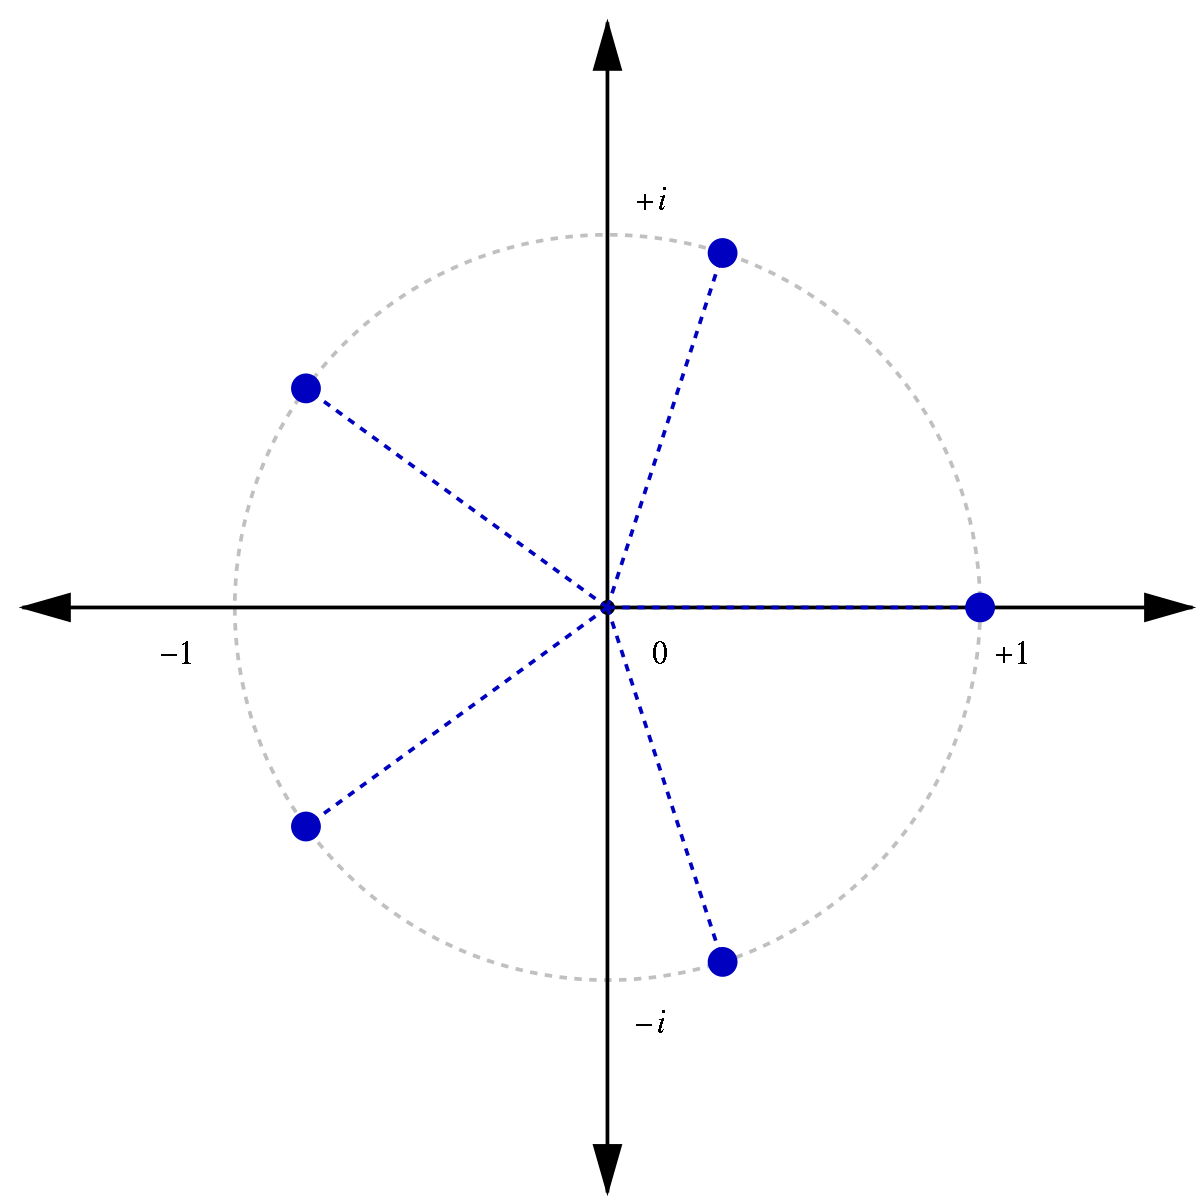
\includegraphics[scale=0.19]{Images/1200px-One5Root.svg.png}
    \caption{Fifth roots of unity}
\end{figure}
\end{example}
In order to finish our characterization of cyclic extensions we need the following lemma.
\begin{lemma}\em
Let $n$ be a positive integer and $K$ a field which contains a primitive $n$-th root of unity $\zeta$.\par
(i) If $d\mid n$, then $\zeta^{n/d}=\eta$ is a primitive $d$-th root of unity in $K$.\par
(ii) If $d\mid n$ and $u$ is a nonzero root of $x^d-a\in K[x]$, then $x^d-a$ has $d$ distinct roots, namely $u$, $\eta u$, $\cdots$, $\eta^{d-1}u$, where $\eta\in K$ is a primitive $d$-th root of unity. Furthermore $K(u)$ is a splitting field of $x^d-a$ over $K$ and is Galois over $K$.
\end{lemma}
\begin{proof}
(i) Suppose $d\mid n$, note that $\eta^d=(\zeta^{n/d})^d=\zeta^n=1_K$, therefore $\eta$ is the $d$-th primitive root of unity.\par
(ii) We first show that $\eta^iu$ is a root of the polynomial $x^d-a\in K[x]$. Note that 
$$
\left( \eta ^iu \right) ^d=\eta ^{id}u^d=\left( \eta ^d \right) ^iu^d=1_{K}^{i}u^d=u^d=a,
$$
whence $u,\eta u,\cdots,\eta^{n-1}u$ are distinct roots of the polynomial $x^d-a$. Now suppose $F=K(u)$, trivially $K(\eta^iu)=K(u)$ since $\zeta\in K$, therefore $K(u)$ is a splitting field of $x^d-a$ over $K$. Note also $F/K$ is separable, we therefore conclude that $F/K$ is a Galois extension.
\end{proof}
\begin{theorem}
Let $n$ be a positive integer and $K$ a field which contains a primitive $n$-th root of unity $\zeta$. Then the following statements are equivalent: \par
(i) $F$ is cyclic over $K$ of degree $d\mid n$;\par
(ii) $F$ is a splitting field over $K$ of a polynomial of the form $x^n-a\in K[x]$. Under which circumstances we have $F=K(u)$, where $u$ is a root of $x^n-a$;\par
(iii) $F$ is a splitting field over $K$ of an irreducible polynomial $x^d-b\in K[x]$. Under which circumstances we have $F=K(v)$, where $v$ is a root of $x^d-b$.
\end{theorem}
\begin{proof}
(ii)$\Rightarrow$(i): Suppose $F$ is a splitting field over $K$ of a polynomial of the form $x^n-a\in K[x]$. By Lemma 6.20 we have $F=K(u)$, where $u$ is a root of $x^n-a$, and $F/K$ is a Galois extension. Now suppose $\sigma\in\mathrm{Gal}(F/K)$, then $\sigma$ is completely determined by $\sigma(u)=\zeta^iu$, where $\zeta$ is the primitive $n$-th unit root. Therefore we may define a homomorphism $\theta:\mathrm{Gal}(F/K)\to\mathbb{Z}_n$ given by $\sigma\mapsto\zeta^i$ provided $\sigma(u)=\zeta^iu$. It is routine to verify $\theta$ is well-defined and a monomorphism. Therefore $\mathrm{Gal}(F/K)$ is a subgroup of $\mathbb{Z}_n$, whence a cyclic group of order $d\mid n$.\par
(i)$\Rightarrow$(iii): Suppose $F$ is cyclic over $K$ of degree $d\mid n$. Then $\mathrm{Gal}(F/K)$ is cyclic. Suppose $\mathrm{Gal}(F/K)=\left<\sigma\right>$. Let $\eta=\zeta^{n/d}$ be the primitive $d$-th root of unity. Note that 
$$
N_{K}^{F}\left( \eta \right) =\eta ^{\left[ F:K \right]}=\left( \zeta ^{n/d} \right) ^d=\zeta ^n=1_K,
$$
we therefore by Hilbert 90 to conclude that there exists some $w\in F$ such that $\eta=w\sigma(w)^{-1}$. Suppose $v=w^{-1}$, we claim that $v^d\in K$. To see this, note that 
$$
\sigma \left( v^d \right) =\sigma \left( v \right) ^d=\left( \eta v \right) ^d=\eta ^dv^d=1_Kv^d=v^d,
$$
whence $v^d$ is fixed by $\sigma$ and hence in $K$. Now suppose $b=v^d$, we have $v$ a root of $x^d-b\in K[x]$, and $K(v)$ is a splitting field over $K$ of $x^d-b$. We further show that $x^d-b$ is irreducible. Consider $\sigma^i:K(u)\to K(\eta^iu)$. Since $\eta^i\in K$, we have $K(u)\cong K(\eta^iu)$ for all $i\in\mathbb{Z}_d$ and hence $x^d-b$ is irreducible. Now it suffices to show that $F=K(v)$. To see this, note that $[K(v):K]=[F:K]=d$, hence $K(v)=F$.\par
(iii)$\Rightarrow$(ii): If $v\in F$ is a root of $x^d-b\in K[x]$, then $F=K(v)$ by Lemma 6.20. Now note that 
$$
\left( \zeta v \right) ^n=\zeta ^nv^n=1_Kv^{d\left( n/d \right)}=b^{n/d}\in K,
$$
therefore $\zeta v$ is a root of $x^n-a\in K[x]$, where $a=b^{n/d}$. By Lemma 6.20 we have $F=K(\zeta v)$ a splitting field of $x^n-a\in K[x]$. However $F=K(v)=K(\zeta v)$ since $\zeta\in K$, which finished the proof.
\end{proof}
It is clear that the primitive $n$-th root of unity plays an important role in the proof of the preceding results. Characterization of the splitting fields of polynomials of the form $x^n-a\in K[x]$ is considerably more difficult when $K$ does not contain a primitive $n$-th root of unity. The case when $a=1_K$ is considered in the next section.
\begin{center}
\begin{large}
    \textbf{Exercises for 6.7}
\end{large}
\end{center}
\begin{problem}\em
If $\overline{K}$ is replaced by any normal extension $N$ of $K$ containing $F$, then this new definition of norm and trace is equivalent to the original one. In particular, the new definition does not depend on the choice of $N$.
\end{problem}
\begin{proof}
Note that if $\overline{K}$ is substituted with $N$, a homomorphism $\sigma:K\to N$ must be a homomorphism $\sigma:K\to\overline{K}$. Therefore it suffices to show that the number of different homomorphisms of $K\to\overline{K}$ and $K\to N$ are the same. Since $\overline{K}$ is normal over $K$ and $\overline{K}\supset F$, then the number of different $\sigma:F\to\overline{K}$ equals to $[F:K]_s$. Similarly we have number of different $\sigma:F\to N$, where $N$ is a normal extension field over $K$ that contains $F$, equals to $[F:K]_s$. Therefore two definitions are equivalent.
\end{proof}
\begin{problem}\em
Let $F$ be a finite dimensional extension of a finite field $K$. The norm ${N_K}^F$ and the trace ${T_K}^F$ (considered as maps $F\to K$) are surjective.
\end{problem}
\begin{proof}
We shall first consider the trace condition. Note that $T_K^F$ is a linear functional, therefore it is either trivial or surjective. Note that if $F$ is a finite dimensional extension of a finite field $K$, then $F/K$ is separable and hence 
$$
T_{K}^{F}\left( u \right) =\left[ F:K \right] _i\cdot \sum_{i=1}^n{\sigma _i\left( u \right)},\hspace{0.5cm}u\in F
$$
is nontrivial, therefore $T_K^F$ is surjective. Note also $N_K^F$ is a linear functional with respect to multiplication, we finished the proof.
\end{proof}
\begin{problem}\em
Let $\overline{\mathbb{Q}}$ be a (fixed) algebraic closure of $\mathbb{Q}$ and $v\in \overline{\mathbb{Q}}, v\notin \mathbb{Q}$. Let $E$ be a subfield of $\overline{\mathbb{Q}}$ maximal with respect to the condition $v\notin E$. Prove that every finite dimensional extension of $E$ is cyclic.
\end{problem}
\begin{proof}
Let $F$ be an extension field of $E$ of finite dimension. We may suppose $F$ is a normal extension field of $E$, or otherwise take the normal closure of $F$ in $E$. Now by definition of $E$ we have $F\supset E(v)$. If $\mathrm{Gal}(F/E)=G$, and the group fixing $E(v)$ is $H$, then $H\subset G$, and any proper subgroup of $G$ is contained in $H$, since for any $E\subset L\subset F$, $L\ne E$, we have $L\supset E(v)$. Therefore if $g\in G$, $g\notin H$, we have the cyclic group $\left<g\right>$ must equal to $G$, hence $G$ is cyclic. This finished the proof.
\end{proof}
\begin{problem}\em
Let $K$ be a field,
$\overline{K}$ an algebraic closure of $K$ and $\sigma\in \mathrm{Gal}(\overline{K}/K)$. Let 
$$F=\{u\in \overline{K}: \sigma(u)=u\}.$$
Then $F$ is a field and every finite dimensional extension of $F$ is cyclic.
\end{problem}
\begin{proof}
$F$ is trivially a field. We now show that if $E/F$ finite dimensional, then $E/F$ is cyclic. Suppose $N/F$ is a normal extension such that $[N:F]<\infty$. It suffices to show that $N/F$ is cyclic. Take $\sigma\in G=\mathrm{Gal}(N/F)$, and let $H=\left<\sigma\right>$ a subgroup of $G$. We now show that $H=G$. Let $N^H$ be the fixed field of $H$, therefore if $x\in H$, then $x$ is fixed by elements in $H$, whence fixed by $\sigma$, hence $x\in F$. Therefore $[N^H:F]=1$, which implies $[G:H]=1$ and hence $G=H$ is cyclic.
\end{proof}
\begin{problem}\em
If $F$ is a cyclic extension of $K$ of degree $p^n$ ($p$ prime) and $L$ is an intermediate field such that $F=L(u)$ and $L$ is cyclic over $K$ of degree $p^{n-1}$, then $F=K(u)$.
\end{problem}
\begin{proof}
Suppose $\mathrm{Gal}(F/K)=\left<\sigma\right>\cong\mathbb{Z}_{p^n}$. Therefore we have $\mathrm{Gal}(F/L)=\left<\sigma^{p^{n-1}}\right>$. Now suppose $\sigma^{p^i}\in\mathrm{Gal}(F/K(u))$, then $\sigma^{p^i}(u)=u$, and hence the only possibility would be $i=n$, which implies $\mathrm{Gal}(F/K(u))$ is trivial. Therefore $F=K(u)$.
\end{proof}
\begin{problem}\em
If $\mathrm{char}F=p\neq 0$, let $K_p=\{u^p-u: u\in K\}$.\par
(i) A cyclic extension field $F$ of $K$ of degree $p$ exists if and only if $K\neq K_p$.\par
(ii) If there exists a cyclic extension of degree $p$ of $K$, then there exists a cyclic extension of degree $p^n$ for every $n\geq 1$.
\end{problem}
\begin{proof}
(i) Suppose there exists an extension field $F$ of $K$ of degree $p$, we prove by contradiction. Suppose $K_p=K$, then $F$ is the splitting field over $K$ of the irreducible polynomial $x^p-x-a\in K[x]$. However since $a\in K$, there exists some $u\in K$ such that $u^p-u=a$, which implies $u$ is a root of $x^p-x-a\in K[x]$, whence the polynomial is not irreducible, a contradiction! Conversely, suppose $K=K_p$, then every polynomial of the form $x^p-x-a\in K[x]$ splits in $K$, whence the only splitting field of $x^p-x-a$ over $K$ are trivial. Hence there are no cyclic extensions of degree $p$ of $K$.\par
(ii) We proof by induction. Suppose $n=1$, then the proposition is trivial. Now if $n>1$, suppose $E/K$ is a cyclic extension of degree $p^{n-1}$ with $\mathrm{Gal}(E/K)=\left<\sigma\right>\cong\mathbb{Z}_{p^{n-1}}$. Now take $z\in E$ such that $T_K^E(z)\ne 0$, define $v=T_K^E(z)^{-1}z$, we have $T_K^E(v)=1_K$ and $v\in E$. Therefore by Hilbert 90 there exists some $u\in E$ such that $\sigma(u)-u=v^p-v$. Now $x^p-x-u\in E[x]$ is irreducible and suppose $w$ is a root of $x^p-x-u$, we have $K(w)$ a desired extension field.
\end{proof}
\begin{problem}\em
If $n$ is an odd integer such that $K$ contains a primitive $n$th root of unity and $\mathrm{char}K\neq 2$, then $K$ also contains a primitive $2n$th root of unity.
\end{problem}
\begin{proof}
Let $\zeta$ be the primitive $n$-th root of unity in $K$. Then consider $-\zeta^2$, which generates a cyclic group of order $2n$ since 
$$
\left( -\zeta ^2 \right) ^{2n}=\left( -1 \right) ^{2n}\left( \zeta ^2 \right) ^{2n}=\zeta ^{4n}=\left( \zeta ^n \right) ^4=1_K,
$$
which finished the proof.
\end{proof}
\begin{problem}\em
Which roots of unity are contained in the following fields: $\mathbb{Q}(\mathrm{i})$, $\mathbb{Q}(\sqrt{2})$, $\mathbb{Q}(\sqrt{3})$, $\mathbb{Q}(\sqrt{5})$, $\mathbb{Q}(\sqrt{-2})$, $\mathbb{Q}(\sqrt{-3})$?
\end{problem}
\begin{proof}
We shall denote $\zeta_n$ the primitive $n$-th root of unity. Note first $\mathbb{Q}(\mathrm{i})$ contains $\zeta_2$ and $\zeta_4$, and $\mathbb{Q}(\sqrt{2})$, $\mathbb{Q}(\sqrt{3})$, $\mathbb{Q}(\sqrt{5})$, as subspaces of $\mathbb{R}$, contains $\zeta_2$. Now we analyze $\mathbb{Q}(\sqrt{-2})$ and $\mathbb{Q}(\sqrt{-3})$. Note first $\mathbb{Q}(\zeta_n)/\mathbb{Q}$ is a cyclic extension field of order $\varphi(n)$, where $\varphi(n)$ is the Euler totient function, and $[\mathbb{Q}(\sqrt{-3}):\mathbb{Q}]=[\mathbb{Q}(\sqrt{-2}):\mathbb{Q}]=2$, we have $\varphi(n)=2$ and hence $n=2,3,4,6$. Note 
$$
\zeta _2=-1,\hspace{0.5cm}\zeta _3=-\frac{1}{2}-\frac{\sqrt{3}}{2}\mathrm{i},\hspace{0.5cm}\zeta _4=\mathrm{i},\hspace{0.5cm}\zeta _6=\frac{1}{2}+\frac{\sqrt{3}}{2}\mathrm{i},
$$
we have $\mathbb{Q}(\sqrt{-2})$ contains $\zeta_2$ and $\mathbb{Q}(\sqrt{-3})$ contains $\zeta_2$, $\zeta_3$ and $\zeta_6$.
\end{proof}
\subsection{Cyclotomic Extensions}
We shall examine splitting fields of the polynomial $x^n-1_K$ in this section, with special attention to the case $K=\mathbb{Q}$.\par
A splitting field $F$ over a field $K$ of $x^n-1_K\in K[x]$ (where $n\ge 1$) is called a \textbf{cyclotomic extension} of order $n$. If $\mathrm{char}K=p\ne 0$ and $n=mp^t$ with $(p,m)=1$, then $x^n-1_K=(x^m-1_K)^{p^t}$ and hence the cyclotomic extension of order $n$ coincides with the one of order $m$. Thus we shall usually assume that $\mathrm{char}K$ does not divide $n$, i.e. $\mathrm{char}K=0$ or $\mathrm{char}K$ is relatively prime to $n$.\par
The dimension of a cyclotomic extension field of order $n$ is related to the \textbf{Euler function} $\varphi(n)$ of elementary number theory, which assigns to each positive integer $n$ the number $\varphi(n)$ of integers $i$ such that $1\le i\le n$ and $(i,n)=1$. For example, $\varphi(6)=2$ and $\varphi(p)=p-1$ provided $p$ is a prime.
\begin{theorem}
Let $n$ be a positive integer, $K$ a field such that $\mathrm{char}K$ does not divide $n$ and $F$ a cyclotomic extension of $K$ of order $n$.\par
(i) $F=K(\zeta)$, where $\zeta\in F$ is a primitive $n$-th root of unity;\par
(ii) $F$ is an abelian extension of dimension $d$, i.e. the $F$ is an algebraic Galois extension of $K$ with $\mathrm{Gal}(F/K)$ abelian, and $d\mid \varphi(n)$, here $\varphi(n)$ is the Euler function. If $n$ is a prime then $F/K$ is a cyclic extension.\par
(iii) $\mathrm{Gal}(F/K)$ is isomorphic to a subgroup of order $d$ of the multiplicative group of units $\mathbb{Z}_n$.
\end{theorem}
\begin{proof}
(i) Note that $F$ contains a primitive $n$-th root of unity $\zeta$. By definition $1_K$, $\zeta$, $\cdots$, $\zeta^{n-1}\in K(\zeta)$ are the $n$ roots of the polynomial $x^n-1_K\in K[x]$, whence $F=K(\zeta)$.\par
(ii) Trivially the polynomial $x^n-1_K$ is separable over $K$, hence $F/K$ is a Galois extension. Suppose $\sigma\in\mathrm{Gal}(F/K)$, then $\sigma$ is completely determined by $\sigma(\zeta)$. For some $i$, we have $\sigma(\zeta)=\zeta^i$ and for some $j$ we have $\sigma^{-1}(\zeta)=\zeta^j$, whence $\zeta=\sigma^{-1}\sigma(\zeta)=\zeta^{ij}$, hence $ij\equiv 1\pmod{n}$. Note that this implies $i$ a unit in $\mathbb{Z}_n$. Consider the homomorphism $\mathrm{Gal}(F/K)\to G$ given by $\sigma\mapsto\overline{\iota}$, where $\overline{\iota}$ is the image of $i$ such that $\sigma(\zeta)=\zeta^i$ in $G$ and $G$ is the multiplicative subgroup of $\mathbb{Z}_n$ consists of all units in $\mathbb{Z}_n$. It is routine to show that the homomorphism is well-defined and a monomorphism. Therefore $\mathrm{Gal}(F/K)\cong\mathrm{Im}f$ is abelian with order $d$ dividing $\varphi(n)$, since $|G|=\varphi(n)$.\par
(iii) has already been proved in (ii). Note that if $n$ is a prime, then $\mathbb{Z}_n$ is a field, and hence $\mathrm{Gal}(F/K)$ is cyclic by Theorem 6.54.
\end{proof}
Let $n$ be a positive integer, $K$ a field such that $\mathrm{char}K$ does not divide $n$, and $F$ a cyclotomic extension of order $n$ of $K$. The \textbf{$n$-th cyclotomic polynomial} over $K$ is the monic polynomial $\Phi_n(x)=(x-\zeta_1)(x-\zeta_2)\cdots(x-\zeta_r)$, where $\zeta_r$ are distinct primitive $n$-th roots of unity in $F$.
\begin{example}\em
It is easily computed some cyclotomic polynomials when $n$ is small. For instance, we have $\Phi_1(x)=x-1_K$, $\Phi_2(x)=(x-(-1_K))=x+1_K$. If $K=\mathbb{Q}$, then we have 
$$
\Phi _3\left( x \right) =\left( x-\left( -\frac{1}{2}+\frac{\sqrt{3}}{2}\mathrm{i} \right) \right) \left( x-\left( -\frac{1}{2}-\frac{\sqrt{3}}{2}\mathrm{i} \right) \right) =x^2+x+1
$$
and 
$$
\Phi _4\left( x \right) =\left( x-\mathrm{i} \right) \left( x+\mathrm{i} \right) =x^2+1.
$$
\end{example}
These examples suggests the following properties of cyclotomic polynomials.
\begin{proposition}
Let $n$ be a positive integer, $K$ a field such that $\mathrm{char}K$ does not divide $n$ and $\Phi_n(x)$ the $n$-th cyclotomic polynomial of $K$.\par
(i) $x^n-1_K=\prod_{d\mid n}\Phi_d(x)$;\par
(ii) The coefficients of $\Phi_n(x)$ lie in the prime subfield $P$ of $K$. If $\mathrm{char}K=0$ and $P$ is identified with the field $\mathbb{Q}$ of rationals, then the coefficients are actually integers.\par
(iii) $\mathrm{deg}\Phi_n(x)=\varphi(n)$, where $\varphi$ is the Euler function.
\end{proposition}
\begin{proof}
(i) Suppose $F/K$ is a cyclotomic extension of order $n$, then $\mathrm{Gal}(F/K)=\left<\zeta\right>$ and hence 
$$
x^n-1_K=\prod_{\eta \in \mathrm{Gal}\left( F/K \right)}{\left( x-\eta \right)}=\prod_{d\mid n}{\prod_{\substack{\eta \in \mathrm{Gal}\left( F/K \right) \\ \left| \eta \right|=d}}{\left( x-\eta \right)}}=\prod_{d\mid n}{\Phi _d\left( x \right)},
$$
which finished the proof.\par
(ii) We proof by induction. For $n=1$, we have $\Phi_1(x)=x-1_K$ and the statement is trivial. Now suppose the statement is true for all $k<n$. Define $f(x)=\prod_{\substack{d\mid n \\ d<n}}\Phi_d(x)$, we therefore have $x^n-1_K=f(x)\Phi_n(x)$ by (i). On the other hand $f(x)$ is monic, and $f\in P[x]$. By the division algorithm over $P[x]$ we have $x^n-1_K=f(x)k(x)+r(x)$, where $k,r\in P[x]\subset F[x]$. However by the uniqueness of division algorithm (over $F[x]$) we must have $r=0$ and $k=\Phi_n$, whence $\Phi_n=k\in P[x]$, which finished the proof. For $K=\mathbb{Q}$, the proof is analogous with $P$ replaced by $\mathbb{Z}$.\par
(iii) Trivially $\mathrm{deg}\Phi_n$ equals to the number of distinct primitive $n$-th roots of unity. Note that if $\zeta$ is a primitive $n$-th root of unity, then $\zeta^k$ is also a primitive $n$-th root of unity if and only if $(k,n)=1$, hence $\mathrm{deg}\Phi_n$ equals to the number of elements in $\{k\in\mathbb{Z}:(k,n)=1\}$, which is precisely $\varphi(n)$.
\end{proof}
\begin{note}\em
Proposition 6.83 offered a recursive method to determine the cyclotomic polynomials. Suppose we would like to calculate $\Phi_6$ over $\mathbb{Q}$. Then since we have already known $\Phi_1$, $\Phi_2$ and $\Phi_3$, we have 
$$
\Phi _6\left( x \right) =\frac{x^n-1}{\prod_{\substack{d\mid n \\ d<n}}{\Phi _d\left( x \right)}}=\frac{x^6-1}{\left( x-1 \right) \left( x+1 \right) \left( x^2+x+1 \right)}=x^2-x+1.
$$
Furthermore, we have 
$$
\Phi _{12}\left( x \right) =\frac{x^{12}-1}{\Phi _1\left( x \right) \Phi _2\left( x \right) \Phi _3\left( x \right) \Phi _6\left( x \right)}=x^4-x^2+1.
$$
\end{note}
We now investigate the cyclotomic polynomials over $\mathbb{Q}$.
\begin{proposition}
Suppose $F$ is a cyclotomic extension field of $\mathbb{Q}$ and $\Phi_n$ the $n$-th cyclotomic polynomial over $\mathbb{Q}$.\par
(i) $\Phi_n(x)$ is irreducible over $\mathbb{Q}[x]$.\par
(ii) $[F:\mathbb{Q}]=\varphi(n)$, where $\varphi$ is the Euler function.\par
(iii) $\mathrm{Gal}(F/\mathbb{Q})$ is isomorphic to the multiplicative group of units in $\mathbb{Z}_n$.
\end{proposition}
\begin{proof}
(i) It suffices to show that $\Phi_n(x)$ is an irreducible monic polynomial over $\mathbb{Z}[x]$. Suppose $h(x)$ is an irreducible factor of $\Phi_n(x)$ over $\mathbb{Z}$, then there exists some $f\in\mathbb{Z}[x]$ such that $\Phi_n(x)=f(x)h(x)$. Suppose $\mathrm{deg}f\ge 1$. Let $\zeta$ be a root of $h$ and $p$ a prime number such that $(p,n)=1$. Since $h$ is an irreducible factor of $\Phi_n$, we have $\zeta$ a primitive $n$-th root of unity. We now claim that $\zeta^p$ is also a root of $h$. Since $\zeta^p$ is also a primitive $n$-th root of unity by $(p,n)=1$, we have $\zeta^p$ either a root of $h$ or a root of $f$. Suppose $\zeta^p$ is a root of $f$, then $\zeta$ is a root of $f(x^p)$. Since $h(x)$ is irreducible over $\mathbb{Q}[x]$, we have $h(x)\mid f(x^p)$ and hence $f(x^p)=h(x)k(x)$ for some $k(x)\in\mathbb{Q}[x]$. Consider the division algorithm in $\mathbb{Z}[x]$ which states $f(x^p)=h(x)k_1(x)+r(x)$, we therefore have $k_1(x)=k(x)\in\mathbb{Z}[x]$. Now we $\bmod{p}$ on both side of $f(x^p)=h(x)k(x)$ and obtain $\overline{f}(x^p)=\overline{f}(x)^p=\overline{h}(x)\overline{k}(x)$, with $\overline{f}\equiv f\pmod{p}$. Now suppose $\overline{l}(x)$ is a irreducible factor of $\overline{h}(x)$, then $\mathrm{l}(x)\mid \overline{f}(x)^p$, whence $\mathrm{l}\mid\overline{f}$ by the unique factorization over $\mathbb{Z}_p[x]$. Now note that $x^n-1_K=\Phi_n(x)m(x)=f(x)h(x)m(x)$, we therefore by $\bmod{p}$ have 
$$
x^n-\overline{1_K}=\overline{x^n-1_K}=\overline{f}\left( x \right) \overline{h}\left( x \right) \overline{m}\left( x \right) .
$$
Note that $\overline{h}(x)$ and $\overline{f}(x)$ have a common divisor $\overline{l}(x)$, which states that $\overline{x^n-1_K}$ has a multiplicative root, a contradiction! Therefore $\zeta^p$ is a root of $h(x)$. Now suppose $r\in\mathbb{Z}$ with $(r,n)=1$, then suppose $r=p_1^{k_1}p_2^{k_2}\cdots p_s^{k_s}$ with $p_i$ prime and $k_i\in\mathbb{Z}_+$, then $(p_i,n)=1$ and hence, using the preceding result repeatedly, $\zeta^r$ is a root of $h$. However this implies $\prod_{\substack{1\le r\le n \\ r\mid n}}(x-\zeta^r)=\Phi_n(x)$ divides $h(x)$, which implies $\Phi_n(x)=h(x)$ and the proof is finished.\par
(ii) Note that 
$$
\left[ F:\mathbb{Q} \right] =\left[ \mathbb{Q} \left( \zeta \right) :\mathbb{Q} \right] =\mathrm{deg}\Phi _n=\varphi \left( n \right) .
$$\par
(iii) Since the multiplicative group of units in $\mathbb{Z}_n$ is of order $\varphi(n)$, and $|\mathrm{Gal}(F/\mathbb{Q})|=\varphi(n)$, we therefore have $\mathrm{Gal}(F/\mathbb{Q})$ is isomorphic to the multiplicative group of units in $\mathbb{Z}_n$.
\end{proof}
A nontrivial theorem of Kronecker states that every abelian extension of $\mathbb{Q}$ is contained in a cyclotomic extension, which we only mention but not proof this result here.
\begin{center}
\begin{large}
    \textbf{Exercises for 6.8}
\end{large}
\end{center}
\begin{problem}\em
If $i\in \mathbb{Z}$, let $\overline{i}$ denote the image of $i$ in $\mathbb{Z}_n$ under the canonical projection $\mathbb{Z}\to \mathbb{Z}_n$. Prove that $\overline{i}$ is a unit in the ring $\mathbb{Z}_n$ if and only if $\gcd{(i, n)}=1$. Therefore the multiplicative group of units in $\mathbb{Z}_n$ has order $\varphi(n)$.
\end{problem}
\begin{problem}\em
Establish the following properties of the Euler function $\varphi$.\par
(a) If $p$ is prime and $n>0$, then $\varphi(p^n)=p^n(1-1/p)=p^{n-1}(p-1)$.\par
(b) If $\gcd{(m, n)}=1$, then $\varphi(mn)=\varphi(m)\varphi(n)$.\par
(c) If $n=p_1^{k_1}\cdots p_r^{k_r}$ ($p_i$ distinct primes; $k_i>0$), then $\varphi(n)=n(1-1/p_1)(1-1/p_2)\cdots (1-1/p_r)$.\par
(d) $\sum_{d\mid n}\varphi(d)=n$.\par
(e) $\varphi(n)=\sum_{d\mid n}d\mu(n/d)$, where $\mu$ is the Moebius function defined by
$$\mu(n)=
\left\{\begin{array}{ll}
1 & \text{if }n=1 \\
(-1)^t & \text{if }n \text{ is a product of }t\text{ distinct primes}\\
0 & \text{if }p^2\text{ divides }n\text{ for some prime }p.
\end{array}\right.
$$
\end{problem}
\begin{problem}\em
Let $\varphi$ be the Euler function.\par
(a) $\varphi(n)$ is even for $n>2$.\par
(b) Find all $n>0$ such that $\varphi(n)=2$.\par
(c) Find all pairs $(n, p)$ (where $n, p>0$, and $p$ is prime) such that $\varphi(n)=n/p$.
\end{problem}
\begin{problem}\em
(a) If $p$ is an odd prime and $n>0$, then the multiplicative group of units in the ring $\mathbb{Z}_{p^n}$ is cyclic of order $p^{n-1}(p-1)$.\par
(b) Part (a) is also true if $p=2$ and $1\leq n\leq 2$.\par
(c) If $n\geq 3$, then the multiplicative group of units in $\mathbb{Z}_{2^n}$ is isomorphic to $\mathbb{Z}_2\oplus \mathbb{Z}_{2^{n-2}}$.
\end{problem}
\begin{problem}\em

\end{problem}
\newpage
\part{Commutative Algebra}
In this part, we shall mainly deal with commutative rings. If stated otherwise, all rings $R$ here are commutative and with an identity. The main reference for this part is Atiyah and MacDonald \textit{An Introduction to Commutative Algebra}. Some other  references are listed below for readers to consult: \par
(a) 
\newpage
\section{More about Rings and Modules}
In this section, we shall introduce some more concepts and properties about rings and ideals.
\subsection{Further Topics on Rings and Ideals}
This section mainly deal with rings. As mentioned in the preface of this part, we only deal with commutative rings unless stated otherwise.
\begin{center}
\begin{large}
    \textbf{Nilradical and Jacobson Radical}
\end{large}
\end{center}
We begin by considering the following proposition: 
\begin{proposition}
The set $\mathfrak{N}$ of all nilpotent elements in a ring $A$ is an ideal, and $A/\mathfrak{N}$ has no nilpotent element $\ne 0$.
\end{proposition}
\begin{proof}
If $x\in\mathfrak{N}$, then there exists some $n\in\mathbb{Z}$ such that $x^n=0$. Therefore for all $a\in A$ we have $(ax)^n=0$. Now it suffices to show that if $x,y\in\mathfrak{N}$, we have $x^m=0$ and $y^n=0$ for some $m,n\in\mathbb{Z}$. Consider $(x+y)^{m+n+1}$, by the binomial theorem (which is valid for commutative rings), we know that $(x+y)^{m+n+1}$ is a sum of $x^sy^t$ with $s+t=m+n+1$. Therefore there must exists $s>m$ or $t>n$, which implies $x+y\in\mathfrak{N}$ and hence $\mathfrak{N}$ an ideal of $A$.\par
Now we show that there are no nilpotent elements in $A/\mathfrak{N}$. Let $a+\mathfrak{N}\in A/\mathfrak{N}$. Suppose there exists some $n\in\mathbb{Z}$ such that $a^n+\mathfrak{N}=0$, then $a^n\in\mathfrak{N}$, whence $a^{nk}=0$ for some $k\in\mathbb{Z}$. This implies $a\in\mathfrak{N}$ and hence the only nilpotent element in $A/\mathfrak{N}$ is $0$.
\end{proof}
The ideal $\mathfrak{N}$ as defined in Proposition 7.1 is called the \textbf{nilradical} of $A$. The following proposition gives an alternative definition of $\mathfrak{N}$:
\begin{proposition}
The nilradical of $A$ is the intersection of all the prime ideals of $A$.
\end{proposition}
\begin{proof}
Let $\mathfrak{P}$ be the set of all prime ideals of $A$ and $\mathfrak{N}=\bigcap_{\mathfrak{p}\in\mathfrak{P}}\mathfrak{p}$. Let $f\in\mathfrak{N}$, then there exists some $n\in\mathbb{Z}$ such that $f^m=0\in\mathfrak{p}$. Since $\mathfrak{p}$ is prime, we have $f\in\mathfrak{p}$. Note that this is true for all $\mathfrak{p}\in\mathfrak{P}$, we have proved $\mathfrak{N}\subset\mathfrak{N}^\prime$. To prove another direction, let $f\notin\mathfrak{N}$. Then for all $n\in\mathbb{Z}$ we have $f^n\ne 0$. Define $\Sigma$ be the set of all ideals $\mathfrak{a}$ of $A$ such that for all $n>0$, $f^n\notin\mathfrak{a}$. Consider $(\Sigma,\subset)$, which by Zorn's lemma, has a maximal element, denote as $\mathfrak{p}$. We shall show $\mathfrak{p}$ is a prime ideal. If not, then there exists some $x,y\notin\mathfrak{p}$ while $xy\in\mathfrak{p}$. Consider the ideals $\mathfrak{p}+(x)$ and $\mathfrak{p}+(y)$, which strictly include the ideal $\mathfrak{p}$ and hence not in $\Sigma$. Therefore there exists $m,n\in\mathbb{Z}$ such that $f^m\in\mathfrak{p}+(x)$ and $f^n\in\mathfrak{p}+(y)$. This implies $f^{m+n}\in\mathfrak{p}+(xy)$, hence the ideal $\mathfrak{p}+(xy)$ is not in $\Sigma$ and $xy\notin\mathcal{p}$, a contradiction! Therefore $\mathfrak{p}$ is a prime ideal and $f\notin\mathfrak{p}$. Therefore for all $f\notin\mathfrak{N}$ we have $f\notin\mathfrak{N}^\prime$, therefore $\mathfrak{N}^\prime\subset\mathfrak{N}$ and hence $\mathfrak{N}=\mathfrak{N}^\prime$.
\end{proof}
The \textbf{Jacobson radical} $\mathfrak{R}$ is defined to be the intersection of all the maximal ideals of $A$. It can be characterized as follows:
\begin{proposition}
Let $\mathfrak{R}$ be the Jacobson radical of the ring $A$, then $x\in\mathfrak{R}$ if and only if $1-xy$ is a unit in $A$ for all $y\in A$.
\end{proposition}
\begin{proof}
Suppose $x\in\mathfrak{R}$. Then if $1-xy$ is not a unit, we have $1-xy\in\mathfrak{m}$ for some maximal ideals $\mathfrak{m}$. Note that $x\in\mathfrak{m}$, therefore $xy\in\mathfrak{m}$ and hence $1\in\mathfrak{m}$, a contradiction! Conversely, if $x\notin\mathfrak{m}$ for some maximal ideal $\mathfrak{m}$. Then the ideal generated by $\mathfrak{m}$ and $x$ is the unit ideal $(1)$. Therefore there exists some $u\in\mathfrak{m}$ and $y\in A$ such that $u+xy=1$, whence $1-xy=u\in\mathfrak{m}$, and hence $1-xy$ is not a unit.
\end{proof}
\begin{center}
\begin{large}
    \textbf{Operations on Ideals}
\end{large}
\end{center}
Recall that the intersection of any family of ideals is an ideal, the product of any family of ideals, which, when there are only two ideals $\mathfrak{a}$ and $\mathfrak{b}$, is defined to be the set of all finite sums $\sum x_iy_i$ with $x_i\in\mathfrak{a}$ and $y_i\in\mathfrak{b}$. The general case may be defined by (possibly transfinite) induction. In particular, if $\mathfrak{a}$ is an ideal, then $\mathfrak{a}^n$ is defined to be the ideal generated by all elements of the form $x_1x_2\cdots x_n$ with each $x_i\in\mathfrak{a}$. Conventionally we denote $\mathfrak{a}^0=1$.
\begin{example}\em
(i) If $A=\mathbb{Z}$, $\mathfrak{a}=(m)$ and $\mathfrak{b}=(n)$, then $\mathfrak{a}\cap\mathfrak{b}$ is the ideal generated by the l.c.m. of $a$ and $b$, and $\mathfrak{a}\mathfrak{b}=(mn)$. Thus in this case $\mathfrak{a}\mathfrak{b}=\mathfrak{a}\cap\mathfrak{b}$ if and only if $m$ and $n$ are coprime.\par
(ii) Let $A=k[x_1,\cdots,x_n]$ and $\mathfrak{a}=(x_1,\cdots,x_n)$ be the ideal generated by $x_1,\cdots,x_n$. Then $\mathfrak{a}^m$ is the set of all polynomials with no terms of degree $<m$.
\end{example}
Two ideals are said to be \textbf{coprime} if $\mathfrak{a}+\mathfrak{b}=(1)$. Therefore for coprime ideals we have $\mathfrak{a}\cap\mathfrak{b}=\mathfrak{a}\mathfrak{b}$. Clearly two ideals $\mathfrak{a}$, $\mathfrak{b}$ are coprime if and only if there exist $x\in\mathfrak{a}$ and $y\in\mathfrak{b}$ such that $x+y=1$. In general, we have the following: 
\begin{proposition}
Let $A$ be a ring and $\mathfrak{a}_1,\cdots,\mathfrak{a}_n$ are ideals of $A$.Define a homomorphism 
$$
\phi :A\rightarrow \bigoplus_{i=1}^n{\left( A/\mathfrak{a} _i \right)}
$$
by the rule $x\mapsto (x+\mathfrak{a}_1,\cdots,x+\mathfrak{a}_n$.\par
(i) If $\mathfrak{a}_i$ and $\mathfrak{a}_j$ are coprime when $i\ne j$, then $\prod\mathfrak{a}_i=\bigcap\mathfrak{a}_i$.\par
(ii) $\phi$ is surjective if and only if $\mathfrak{a}_i$ and $\mathfrak{a}_j$ are coprime when $i\ne j$, and $\phi$ is injective if and only if $\bigcap\mathfrak{a}_i=(0)$.
\end{proposition}
\begin{proof}
(i) We prove by induction. Suppose $\mathfrak{a}_i$ and $\mathfrak{a}_j$ coprime, we first show that $\mathfrak{a}_i\mathfrak{a}_j=\mathfrak{a}_i\cap\mathfrak{a}_j$. Trivially $\mathfrak{a}_i\mathfrak{a}_j\subset\mathfrak{a}_i\mathfrak{a}_j$. For the converse inclusion, let $x_i\in\mathfrak{a}_i$ and $x_j\in\mathfrak{a}_j$ such that $x_i+x_j=1$. Then $x=xx_i+xx_j\in\mathfrak{a}_i\mathfrak{a}_j$. To prove the general case, suppose the result is true for $k<n$. Therefore suppose $\mathfrak{a}_1,\cdots,\mathfrak{a}_k$ are pairwise coprime, define $\mathfrak{b}=\prod_{i=1}^k\mathfrak{a}_i=\bigcap_{i=1}^k\mathfrak{a}_i$. Since $\mathfrak{a}_i+\mathfrak{a}_k=(1)$ we have $x_i\in\mathfrak{a}_i,y_i\in\mathfrak{a}_k$ such that $x_i+y_i=1$. Therefore 
$$
\prod_{i=1}^{k-1}{x_i}=\prod_{i=1}^{k-1}{\left( 1-y_i \right)}\equiv 1\left( \mathrm{mod}\ \mathfrak{a} _k \right) .
$$
Hence $x=\prod_{i=1}^{k-1}x_i-1\in\mathfrak{a}_k$, whence there exists some $-y\in\mathfrak{a}_k$ such that $x-1=-y$, therefore $x+y=1$ and hence $\mathfrak{a}_k$ and $\mathfrak{b}$ coprime. Therefore 
$$
\mathfrak{b} \mathfrak{a} _k=\left( \prod_{i=1}^{k-1}{\mathfrak{a} _i} \right) \mathfrak{a} _k=\prod_{i=1}^k{\mathfrak{a} _i}=\left( \bigcap_{i=1}^{k-1}{\mathfrak{a} _i} \right) \cap \mathfrak{a} _k=\bigcap_{i=1}^k{\mathfrak{a} _k}.
$$
The proof is therefore finished via induction.\par
(ii) We first note that $\mathrm{Ker}\phi=\bigcap\mathfrak{a}_i$, therefore $\bigcap\mathfrak{a}_i=(0)$ if and only if $\phi$ is surjective. To prove the last condition, we first suppose $\phi$ surjective. We show that $\mathfrak{a}_i$ and $\mathfrak{a}_j$ are coprime. Let $x\in A$ such that 
$$
\phi \left( x \right) =\left( 0,\cdots ,1+\mathfrak{a} _i,\cdots ,0 \right) ,
$$
then $1-x\in\mathfrak{a}_i$ and $x\in\mathfrak{a}_j$. Therefore $1=1-x+x\in\mathfrak{a}_i+\mathfrak{a}_j$. Conversely, suppose $\mathfrak{a}_i$ and $\mathfrak{a}_j$ coprime when $i\ne j$. Then $\mathfrak{a}_i$ is coprime with $\prod_{j\ne i}\mathfrak{a}_j$. Let $x_i\in\mathfrak{a}_i$ and $y_i\in\prod_{j\ne i}\mathfrak{a}_j$ such that $x_i+y_i=1$, therefore $y_i\equiv 1(\mathrm{mod}\mathfrak{a}_i)$. Now for each $(r_1+\mathfrak{a}_1,\cdots,r_n+\mathfrak{a}_n)$, let $x=\sum r_iy_i$.
\end{proof}
\begin{note}\em
Such a homomorphism $\phi$ is called the \textbf{standard homomorphism} with respect to the ideal $\mathfrak{a}$ in $A$.
\end{note}
In general, $\mathfrak{a}\cup\mathfrak{b}$ is not an ideal.
\begin{proposition}
(i) Let $\mathfrak{p}_1,\cdots,\mathfrak{p}_n$ be prime ideals and let $\mathfrak{a}$ be an ideal contained in $\bigcup_{i=1}^n\mathfrak{p}_i$. Then $\mathfrak{a}\subset\mathfrak{p}_i$ for some $i$.\par
(ii) Let $\mathfrak{a}_1,\cdots,\mathfrak{a}_n$ be ideals and let $\mathfrak{p}$ be a prime ideal containing $\bigcap_{i=1}^n\mathfrak{a}_i$, then $\mathfrak{p}\supset\mathfrak{a}_i$ for some $i$. If $\mathfrak{p}=\bigcap\mathfrak{a}_i$, then $\mathfrak{p}=\mathfrak{a}_i$ for some $i$.
\end{proposition}
\begin{proof}
(i) It suffices to show that if $\mathfrak{a}\not\subset\mathfrak{p}_i$ for all $i$, then $\mathfrak{a}$ is not contained in $\bigcup_{i=1}^n\mathfrak{p}_i$.
We prove by induction. Suppose $i=1$, then the condition is trivial. Now if the statement is true when $k=n-1$, then we may take $x_i\in\mathfrak{a}$ such that $x_i\notin\mathfrak{p}_j$ for all $j\ne i$. Now if each $x_i\notin\mathfrak{p}_i$, then the proof is done. Otherwise consider 
$$
x=\sum_{i=1}^n{\prod_{j\ne i}{x_j}},
$$
therefore $x\in\mathfrak{a}$ and $x\notin\mathfrak{p}_i$, this finished the proof.\par
(ii) Suppose $\mathfrak{p}\not\supset\mathfrak{a}_i$ for all $i$. Therefore there exists $x_i\in\mathfrak{a}_i$ such that $x_i\in\mathfrak{a}_i$ and $x_i\notin\mathfrak{p}$. Since $\mathfrak{p}$ is prime, $\prod_{i=1}^nx_i\notin\inf{p}$. However $\prod_{i=1}^nx_i\in\bigcap_{i=1}^n\mathfrak{a}_i$, a contradiction! If $\mathfrak{p}=\bigcap\mathfrak{a}_i$, then $\mathfrak{p}\supset\mathfrak{a}_i$ for some $i$ by previous discussion. However $\mathfrak{p}\subset\mathfrak{a}_i$ by the hypothesis, which implies $\mathfrak{p}=\mathfrak{a}_i$ for some $i$.
\end{proof}
If $\mathfrak{a}$ and $\mathfrak{b}$ are two ideals in a ring $A$, then their \textbf{ideal quotient} is defined to be 
$$(\mathfrak{a}:\mathfrak{b})=\{x\in A:x\mathfrak{b}\subset\mathfrak{a}\}$$
which is an ideal. In particular, $(0:\mathfrak{b})$ is called the \textbf{annihilator} of $\mathfrak{b}$ and is also denoted by $\mathrm{Ann}(\mathfrak{b})$. If $(x)$ is a principal ideal, then we will write $(\mathfrak{a}:x)$ instead of $(\mathfrak{a}:(x))$. In this notation, the set of all zero-divisors of a ring $A$ is 
$$
D=\bigcap_{x\ne 0}{\mathrm{Ann}\left( x \right)}.
$$
We define the \textbf{radical} of an ideal $\mathfrak{a}$ as 
$$r(\mathfrak{a})=\{x\in A:x^n\in\mathfrak{a}\ \text{for some}\ n>0\}.$$
Clearly $r(\mathfrak{a})$ is still an ideal of $A$. Consider $\phi^{-1}(\mathfrak{N}_{A/\mathfrak{a}})$, where $\phi$ is the standard homomorphism.
\begin{center}
\begin{large}
    \textbf{Extension and Contraction}
\end{large}
\end{center}
Let $f:A\to B$ be a ring homomorphism. If $\mathfrak{a}$ is an ideal in $A$, the set $f(\mathfrak{a})$ need not be an ideal. For example, consider $f:\mathbb{Z}\to\mathbb{Q}$ canonical injection, and take $\mathfrak{a}$ be a nonzero ideal of $\mathbb{Z}$. We define the \textbf{extension} $\mathfrak{a}^e$ of $\mathfrak{a}$ to be the ideal $Bf(\mathfrak{a})$ generated by $f(\mathfrak{a})$, i.e. $\mathfrak{a}^e$ is the set of all elements of the form $\sum y_if(x_i)$ where $y_i\in B$ and $x_i\in\mathfrak{a}$.\par
If $\mathfrak{b}$ is an ideal, then $f^{-1}(\mathfrak{b})$ is always an ideal of $A$, called the \textbf{contraction} $\mathfrak{b}^c$ of $\mathfrak{b}$. If $\mathfrak{b}$ is prime, then $\mathfrak{b}^c$ is also a prime. However this is generally not true for extensions.\par
We can factorize $f$ as follows: 
$$
A\overset{p}{\longrightarrow}f\left( A \right) \overset{j}{\longrightarrow}B,
$$
where $p$ is projective and $j$ is injective. For $p$ the condition is very simple, there is a one-to-one correspondence between ideals of $f(A)$ and ideals of $A$ that contains $\mathrm{Ker}f$. For $j$, the condition is very complicated. The classical example is from algebraic number theory.
\begin{example}\em
Consider $\mathbb{Z}\to\mathbb{Z}[\mathrm{i}]$, where $\mathrm{i}=\sqrt{-1}$. A prime ideal $(p)$ in $\mathbb{Z}$ may or may not stay prime when extended to $\mathbb{Z}[\mathrm{i}]$. Since $\mathbb{Z}[\mathrm{i}]$ is a principal ideal domain, we have the following facts: \par
(i) $(2)^e=((1+\mathrm{i})^2)$, which is a square of a prime ideal in $\mathbb{Z}[\mathrm{i}]$.\par
(ii) If $p\equiv 1(\mathrm{mod}4)$ then $(p)^e$ is the product of two distinct prime ideals. For example, $(5)=(2+\mathrm{i})(2-\mathrm{i})$ in $\mathbb{Z}[\mathrm{i}]$.\par
(iii) If $p\equiv 3(\mathrm{mod}4)$ then $(p)^e$ is a prime in $\mathbb{Z}[\mathrm{i}]$.
\end{example}
\begin{note}\em
The proof of these consequences are not trivial. In fact the behavior of prime ideals under extensions of this sort is one of the central problems of algebraic number theory.
\end{note}
\begin{proposition}
Let $f:A\to B$, $\mathfrak{a}$ and $\mathfrak{b}$ be as before. Then \par
(i) $\mathfrak{a}\subset\mathfrak{a}^{ec}$, $\mathfrak{b}\supset\mathfrak{b}^{ce}$.\par
(ii) $\mathfrak{b}^c=\mathfrak{b}^{cec}$, $\mathfrak{a}^e=\mathfrak{a}^{ece}$.\par
(iii) If $C$ is the set of contracted ideals in $A$ and if $E$ is the set of extended ideals in $B$, then $C=\{\mathfrak{a}:\mathfrak{a}^{ec}=\mathfrak{a}\}$, $E=\{\mathfrak{b}:\mathfrak{b}^{ce}=\mathfrak{b}\}$, and $\mathfrak{a}\mapsto\mathfrak{a}^e$ is a bijective map of $C$ onto $E$, whose inverse is $\mathfrak{b}\mapsto\mathfrak{b}^c$.
\end{proposition}
\begin{proof}
(i) Suppose $a\in\mathfrak{a}$, then $f(a)\in\mathfrak{a}^e$, and $a=f^{-1}(f(a))\in\mathfrak{a}^{ec}$, therefore $\mathfrak{a}\subset\mathfrak{a}^{ec}$. The proof is similar for $\mathfrak{b}$.\par
(ii) Note that $\mathfrak{b}^c\subset\mathfrak{b}^{cec}\subset\mathfrak{b}^c$, therefore $\mathfrak{b}^c=\mathfrak{b}^{cec}$. The proof is similar for $\mathfrak{a}$.\par
(iii) Suppose $\mathfrak{a}\in C$. Then there exists some $\mathfrak{b}$ such that $\mathfrak{b}^c=\mathfrak{a}$. Therefore $\mathfrak{a}=\mathfrak{b}^c=\mathfrak{b}^{cec}=\mathfrak{a}^ec$. The proof is similar to $E$.
\end{proof}
\subsection{Exercises about Rings}
In this section we give further information on rings in the form of exercises (with solutions). Each group of exercises is devoted to proof or introduce one theme exclude miscellaneous problems.
\begin{center}
\begin{large}
    \textbf{The Prime Spectrum of a Ring}
\end{large}
\end{center}
\begin{problem}\em
Let $A$ be a ring and let $X$ be the set of all prime ideals of $A$. For each subset $E$ of $A$, let $V(E)$ denote the set of all prime ideals of $A$ which contain $E$. Prove that \par
(i) If $\mathfrak{a}$ is a prime ideal generated by $E$, then $V(E)=V(\mathfrak{a})=V(r(\mathfrak{a}))$.\par
(ii) $V(0)=X$, $V(1)=\emptyset$.\par
(iii) If $\{E_i\}_{i\in I}$ is a family of subsets of $A$, then 
$$
V\left( \bigcup_{i\in I}{E_i} \right) =\bigcap_{i\in I}{V\left( E_i \right)}.
$$\par
(iv) $V(\mathfrak{a}\cap\mathfrak{b})=V(\mathfrak{a}\mathfrak{b})=V(\mathfrak{a})\cup V(\mathfrak{b})$ for any ideals $\mathfrak{a},\mathfrak{b}\in A$.
\end{problem}
\begin{proof}
(i) Note that $E\subset\mathfrak{a}$, therefore $V(E)\supset V(\mathfrak{a})$. For the converse inclusion, suppose $\mathfrak{p}\in V(E)$. Then $E\subset\mathfrak{p}$. Since $\mathfrak{p}$ is an ideal, we have $(E)=\mathfrak{a}\subset\mathfrak{p}$, hence $\mathfrak{p}\in V(\mathfrak{a})$. This gives $V(E)=V(\mathfrak{a})$.\par
For the second equality, note that $\mathfrak{a}\subset r(\mathfrak{a})$, therefore $V(r(\mathfrak{a}))\subset V(\mathfrak{a})$. For the converse inclusion, suppose $\mathfrak{p}\in V(\mathfrak{a})$. Then $\mathfrak{p}\supset\mathfrak{a}$ and hence $r(\mathfrak{p})=\mathfrak{p}\supset r(\mathfrak{a})$. Therefore $\mathfrak{p}\in V(r(\mathfrak{a}))$ and hence $V(\mathfrak{a})=V(r(\mathfrak{a}))$.\par
(ii) This is trivial by definition.\par
(iii) Suppose $\mathfrak{p}\in V\left(\bigcup_{i\in I}E_i\right)$. Then $\mathfrak{p}\supset\bigcup_{i\in I}E_i$, and hence $\mathfrak{p}\supset E_i$ for all $i\in I$. This implies $\mathfrak{p}\in V(E_i)$ for all $i\in I$, which is $\mathfrak{p}\in\bigcap_{i\in I}V(E_i)$. For the converse inclusion, suppose $\mathfrak{p}\in\bigcap_{i\in I}V(E_i)$. Then by an analogous discussion we have 
$$
V\left( \bigcup_{i\in I}{E_i} \right) =\bigcap_{i\in I}{V\left( E_i \right)}.
$$\par
(iv) It suffices to note that 
$$
V\left( \mathfrak{a} \mathfrak{b} \right) =\left\{ \mathfrak{p} \in X:\mathfrak{a} \mathfrak{b} \subset \mathfrak{p} \right\} =\left\{ \mathfrak{p} \in X:\mathfrak{a} \subset \mathfrak{p} \right\} \cup \left\{ \mathfrak{p} \in X:\mathfrak{b} \subset \mathfrak{p} \right\} =V\left( \mathfrak{a} \right) \cup V\left( \mathfrak{b} \right) ,
$$
where the second equality follows from the fact that $\mathfrak{p}$ is prime.
\end{proof}
\begin{note}\em
The result of the preceding exercise shows that the sets $V(E)$ satisfy the axioms for closed sets in a topological space. The resulting topology is called the \textbf{Zariski topology}. The topological space $X$ is called the \textbf{prime spectrum} of $A$, and is written $\mathrm{Spec}(A)$.
\end{note}
\begin{problem}\em
Draw pictures of $\mathrm{Spec}(\mathbb{Z})$, $\mathrm{Spec}(\mathbb{R})$, $\mathrm{Spec}(\mathbb{C}[x])$, $\mathrm{Spec}(\mathbb{R}[x])$ and $\mathrm{Spec}(\mathbb{Z}(x))$.
\end{problem}
\begin{proof}
For $\mathrm{Spec}(\mathbb{Z})$, we have 
$$
\mathrm{Spec}(\mathbb{Z})=\{(p): p\ \text{is a prime number in}\ \mathbb{Z}\}\cup\{0\}.
$$
The closed sets in $\mathrm{Spec}(\mathbb{Z})$ are $0$ and finite sets of prime ideals.\par
For $\mathrm{Spec}(\mathbb{R})$, since $\mathbb{R}$ is a field, the only ideal of $\mathbb{R}$ is $0$. Therefore $\mathrm{Spec}(\mathbb{R})=0$ and the topology on $\mathrm{Spec}(\mathbb{R})$ is discrete.\par
For $\mathrm{Spec}(\mathbb{C}[x])$, since $\mathbb{C}$ is algebraically closed, every polynomial splits in $\mathbb{C}$. Therefore 
$$
\mathrm{Spec}(\mathrm{C}[x])=\{(x-a):a\in\mathbb{C}\}\cup\{0\}.
$$
The closed sets in $\mathrm{Spec}(\mathbb{C}[x])$ are $0$ and finite sets of prime ideals.\par
For $\mathrm{Spec}(\mathbb{R}[x])$, since every polynomial in $\mathbb{R}[x]$ can be break into parts with degree less than $2$, and the parts of degree $2$ may be factored as $(x-a)(x+a)$ with $a\in\mathbb{C}_+$, where $\mathbb{C}_+$ denote elements $z$ of positive imaginary parts, we have 
$$
\mathrm{Spec}(\mathbb{R}[x])=\{(x-a):a\in\mathbb{R}\}\cup\{(x-a)(x+a):a\in\mathbb{C}_+\}\cup\{0\}.
$$
The closed sets in $\mathrm{Spec}(\mathbb{R}[x])$ are $0$ and finite sets of irreducible polynomials in $\mathbb{R}[x]$.\par
For $\mathrm{Spec}(\mathbb{Z}[x])$, we claim that 
$$
\begin{aligned}
&\mathrm{Spec}(\mathbb{Z}[x])=
\\
&\{(p(x)):p(x)\ \text{is irreducible on}\ \mathbb{Z}[x]\}\cup\{(p,p(x)):p\ \text{prime in}\ \mathbb{Z}, p(x)\ \text{is irreducible on}\ \mathbb{Z}[x]\}\cup\{0\}.
\end{aligned}
$$
To prove this, we consider the morphism $\mathrm{Spec}(\mathbb{Z}[x])\to\mathrm{Spec}(\mathbb{X})$ defined by the inclusion map $\mathbb{Z}\to\mathbb{Z}[x]$, it suffices to determine the fiber of this map. Now for $(p)\subset\mathbb{Z}$ a prime ideal, we consider the pullback given by the following commutative diagram: 
\begin{center}


\tikzset{every picture/.style={line width=0.75pt}} %set default line width to 0.75pt        

\begin{tikzpicture}[x=0.75pt,y=0.75pt,yscale=-1,xscale=1]
%uncomment if require: \path (0,476); %set diagram left start at 0, and has height of 476

%Straight Lines [id:da4576996492347125] 
\draw    (248,192) -- (334,192) ;
\draw [shift={(336,192)}, rotate = 180] [color={rgb, 255:red, 0; green, 0; blue, 0 }  ][line width=0.75]    (10.93,-3.29) .. controls (6.95,-1.4) and (3.31,-0.3) .. (0,0) .. controls (3.31,0.3) and (6.95,1.4) .. (10.93,3.29)   ;
%Straight Lines [id:da088557734678675] 
\draw    (216,208) -- (216,262) ;
\draw [shift={(216,264)}, rotate = 270] [color={rgb, 255:red, 0; green, 0; blue, 0 }  ][line width=0.75]    (10.93,-3.29) .. controls (6.95,-1.4) and (3.31,-0.3) .. (0,0) .. controls (3.31,0.3) and (6.95,1.4) .. (10.93,3.29)   ;
%Straight Lines [id:da7521559935110449] 
\draw    (384,208) -- (384,262) ;
\draw [shift={(384,264)}, rotate = 270] [color={rgb, 255:red, 0; green, 0; blue, 0 }  ][line width=0.75]    (10.93,-3.29) .. controls (6.95,-1.4) and (3.31,-0.3) .. (0,0) .. controls (3.31,0.3) and (6.95,1.4) .. (10.93,3.29)   ;
%Straight Lines [id:da9763436140563071] 
\draw    (240,272) -- (350,272) ;
\draw [shift={(352,272)}, rotate = 180] [color={rgb, 255:red, 0; green, 0; blue, 0 }  ][line width=0.75]    (10.93,-3.29) .. controls (6.95,-1.4) and (3.31,-0.3) .. (0,0) .. controls (3.31,0.3) and (6.95,1.4) .. (10.93,3.29)   ;

% Text Node
\draw (174,264.4) node [anchor=north west][inner sep=0.75pt]    {$\text{Spec}(\mathbb{Z}[ x])$};
% Text Node
\draw (352,264.4) node [anchor=north west][inner sep=0.75pt]    {$\text{Spec}(\mathbb{Z})$};
% Text Node
\draw (170,184.4) node [anchor=north west][inner sep=0.75pt]    {$\text{Spec}( \kappa ( p)[ x])$};
% Text Node
\draw (336,184.4) node [anchor=north west][inner sep=0.75pt]    {$\text{Spec}(\mathbb{Z} /( p))$};


\end{tikzpicture}
\end{center}
Therefore for $(0)$, the fiber over it is $\mathrm{Spec}(\mathbb{Q}\otimes_{\mathbb{Z}}\mathbb{Z}[x])=\mathrm{Spec}(\mathbb{Q}(x))$, which consists of irreducible polynomials in $\mathbb{Q}[x]$. For $(p)$, on the other hand, the fiber over it is $\mathrm{Spec}(\mathbb{Z}_p[x])$, which is just irreducible polynomials over $\mathbb{Z}_p[x]$ and the zero ideal (corresponds to those in $\mathbb{Z}$).
\end{proof}
\begin{note}\em
We used the language of Algebraic Geometry to characterize $\mathrm{Spec}(\mathbb{Z}[x])$. Indeed one may use only Abstract Algebra to solve this. One may consider a prime ideal $\mathfrak{p}$ intersect with $\mathbb{Z}$, and transform the language of Algebraic Geometry into Abstract Algebra, which is more elementary but with cumbersome details.
\end{note}
\begin{problem}\em
For each $f\in A$, let $X_f$ denote the complement of $V(f)$ in $X=\mathrm{Spec}(A)$. The sets $X_f$ are open. Show that they form a basis of open sets for the Zariski topology, and that \par
(i) $X_f\cap X_g=X_{fg}$;\par
(ii) $X_f=\emptyset$ if and only if $f$ is nilpotent;\par
(iii) $X_f=X$ if and only if $f$ is a unit;\par
(iv) $X_f=X_g$ if and only if $r((f))=r((g))$;\par
(v) $X$ is quasi-compact;\par
(vi) More generally, each $X_f$ is quasi-compact;\par
(vii) An open subset of $X$ is quasi-compact if and only if it is a finite union of sets $X_f$.
\end{problem}
\begin{proof}
Trivially $\emptyset$ and $\mathrm{Spec}(A)\in\{X_f\}_{f\in A}$. The fact that every prime ideal $\mathfrak{p}$ in the intersection of two elements has a neighborhood in $\{X_f\}_{f\in A}$ follows from (i) below.\par
(i) This is trivial once observe that $X_f\cap X_g=(V(f)\cup V(g))^c=(V(fg))^c=X_{fg}$.\par
(ii) Suppose $X_f=\emptyset$, then $V(f)=\mathrm{Spec}(A)$. Hence for all $\mathfrak{p}\in\mathrm{Spec}(A)$ we have $f\subset\mathfrak{p}$, therefore 
$$
f\in \bigcap_{\mathfrak{p} \in \mathrm{Spec}\left( A \right)}{\mathfrak{p}}=\mathfrak{N} .
$$
Therefore $f$ is nilpotent. Conversely, if $f$ is nilpotent, then $f\in\mathfrak{N}$ and hence $f$ lies in every prime ideal of $A$, hence $V(f)=\mathrm{Spec}(A)$.\par
(iii) Suppose $X_f=X$, then $V(f)=\emptyset$. Therefore $f$ does not lie in any prime ideal, which includes maximal ideals. Therefore $f$ is a unit. Conversely if $f$ is a unit, then $V(f)$ is the set of all prime ideals that contain the whole space, which is the null set.\par
(iv) Suppose $X_f=X_g$. We may also suppose that both $f$ and $g$ are ideals. Therefore 
$$
r\left( f \right) =\bigcap{\left\{ \mathfrak{p} \in \mathrm{Spec}\left( A \right) :f\subset \mathfrak{p} \right\}}\subset \bigcap{\left\{ \mathfrak{p} \in \mathrm{Spec}\left( A \right) :g\subset \mathfrak{p} \right\}}=r\left( g \right) .
$$
Therefore $r(f)\subset r(g)$. However the converse inclusion is also true by a symmetric procedure, hence $r(f)=r(g)$. Now for another direction, if $r(f)=r(g)$, then 
$$
\bigcap{\left\{ \mathfrak{p} \in \mathrm{Spec}\left( A \right) :f\subset \mathfrak{p} \right\}}=\bigcap{\left\{ \mathfrak{p} \in \mathrm{Spec}\left( A \right) :g\subset \mathfrak{p} \right\}},
$$
which implies that the prime ideals $\mathfrak{p}$ of $A$ that containing $f$ coincide with those containing $g$, whence $X_f=X_g$.\par
(v) Suppose $\{X_f\}_{f\in I}$ is a cover of $\mathrm{Spec}(A)$. Then 
$$
\bigcup_{f\in I}{X_f}=\bigcup_{f\in I}{\left( V\left( f \right) \right) ^c}=\left( \bigcap_{f\in I}{V\left( f \right)} \right) ^c.
$$
Therefore 
$$
\bigcap_{f\in I}{V\left( f \right)}=\emptyset .
$$
We claim that $1\in I$. Suppose not, then there exists some maximal ideal $\mathfrak{m}$ such that $\mathfrak{m}\in\bigcap_fV(f)$, a contradiction. Hence $1=\sum_{j=1}^na_jf_j$ for a linear combination of a finite many elements in $I$. Hence 
$$
\mathrm{Spec}\left( A \right) =\left( \bigcap_{i=1}^n{V\left( f_i \right)} \right) ^c=\bigcup_{i=1}^n{X_{f_i}}
$$
is a subcover of $\mathrm{Spec}(A)$, whence $\mathrm{Spec}(A)$ is quasi-compact.\par
(vi) Suppose $\{X_{f_i}\}_{i\in I}$ is a cover of $X_f$. Then 
$$
X_f=\bigcup_{i\in I}{\left( X_{f_i}\cap X_f \right)}=\bigcup_{i\in I}{X_{ff_i}}.
$$
To simplify the notations, we shall write $ff_i$ as $f_i$. Now 
$$
X_f=\left( V\left( f \right) \right) ^c=\bigcup_{i\in I}{\left( V\left( f_i \right) \right) ^c}=\left( \bigcap_{i\in I}{V\left( f_i \right)} \right) ^c,
$$
hence 
$$
V\left( f \right) =\bigcap_{i\in I}{V\left( f_i \right)}.
$$
Therefore $r(f)=r(\{f_i\}_{i\in I})$ and hence $f^n=\sum_{j=1}^ma_jf_j$ for a finite many elements in $I$. Therefore 
$$
f^n=\sum_{j=1}^m{a_jf_j}\in \bigcap_{i\in I}{V\left( f_i \right)}=V\left( f \right) .
$$
Note that if $f^n\in\mathfrak{p}$, then $f\in\mathfrak{p}$ since $\mathfrak{p}$ is prime. Hence 
$$
V\left( f \right) \supset \bigcap_{j=1}^m{V\left( f_j \right)}=V\left( \bigcup_{j=1}^m{f_j} \right) .
$$
Hence $\{x_{f_j}\}_{j=1}^m$ is a subcover of $X_f$ and hence $X_f$ is quasi-compact.\par
(vii) If an open set $O$ is a finite union of sets $X_f$, then clearly it is quasi-compact. Now we prove the converse. Since $\{X_f\}_{f\in A}$ is an open basis of $\mathrm{Spec}(A)$, we may choose (maybe infinitely many) $\{X_{f_i}\}_{i\in I}$ to be an open cover of $O$ such that $O=\bigcup_iX_{f_i}$. Since $O$ is quasi-compact, there are finitely many $\{X_{f_j}\}_{j=1}^n$ that forms a subcover. Therefore 
$$
O\subset \bigcup_{j=1}^n{X_{f_j}}\subset \bigcup_{i\in I}{X_{f_i}}=O,
$$
which finished the proof.
\end{proof}
\begin{note}\em
The sets $X_f$ are called \textbf{basic open sets} of $X=\mathrm{Spec}(A)$.
\end{note}
\begin{problem}\em
It is sometimes convenient to denote a prime ideal of $A$ by a letter such as $x$ or $y$ when thinking of it as a point of $X=\mathrm{Spec}(A)$. When thinking of $x$ as a prime ideal of $A$, we denote it by $\mathfrak{p}_x$. Show that \par
(i) The set $\{x\}$ is closed (we say $x$ a closed point) in $\mathrm{Spec}(A)$ if and only if $\mathfrak{p}_x$ is maximal;\par
(ii) $\overline{\{x\}}=V(\mathfrak{p}_x)$;\par
(iii) $y\in\overline{\{x\}}$ if and only if $\mathfrak{p}_x\subset\mathfrak{p}_y$;\par
(iv) $X$ is a $T_0$-space.
\end{problem}
\begin{proof}
(i) Suppose $\{x\}$ is closed. Then the set $V(\mathfrak{p})=\{x\}$ for some $\mathfrak{p}$. This is possible only if $\mathfrak{p}=\mathfrak{p}_x$ is a maximal ideal. Conversely, if $\mathfrak{p}_x$ is a maximal ideal, then $\{x\}=V(\mathfrak{p}_x)$ is closed.\par
(ii) By definition of a closure, we have 
$$
\overline{\left\{ x \right\} }=\bigcap{\left\{ \mathfrak{p} \in \mathrm{Spec}\left( A \right) :\mathfrak{p} _x\in V\left( \mathfrak{p} \right) \right\}}=\bigcap{\left\{ V\left( \mathfrak{p} \right) :\mathfrak{p} \subset \mathfrak{p} _x \right\}}=V\left( \mathfrak{p} _x \right) .
$$\par
(iii) Suppose $y\in\overline{\{x\}}$, then $\mathfrak{p}_y\in V(\mathfrak{p}_x)$ and hence $\mathfrak{p}_x\subset\mathfrak{p}_y$.\par
(iv) Suppose $x$ and $y$ are distinct points in $\mathrm{Spec}(A)$. Then if $y$ lies in every neighborhood of $x$ and vice versa, we have $\mathfrak{p}_x\subset\mathfrak{p}_y\subset\mathfrak{p}_x$, hence $x=y$, a contradiction.
\end{proof}
\begin{problem}\em
A topological space $X$ is said to be \textbf{irreducible} if $X\ne\emptyset$ and if every pair of non-empty open sets in $X$ intersect, or equivalently if every non-empty open set is dense in $X$. Show that $\mathrm{Spec}(A)$ is irreducible if and only if the nilradical of $A$ is a prime ideal.
\end{problem}
\begin{proof}
Suppose $\mathrm{Spec}(A)$ is irreducible, then for arbitrary nonempty two open sets, say $O_1$ and $O_2$, there intersection is nonempty. Since $\{X_f\}_{f\in A}$ is a basis of $\mathrm{Spec}(A)$, we may suppose $O_1=X_f$ and $O_2=X_g$. Therefore $X_f\cap X_g=X_{fg}$ is nonempty. Therefore $f,g\notin\mathfrak{N}$ implies $fg\notin\mathfrak{N}$, whence $\mathfrak{N}$ is a prime ideal. Conversely, if $\mathfrak{N}$ is a prime ideal, then if $fg\in\mathfrak{N}$, we have $f\in\mathfrak{N}$ or $g\in\mathfrak{N}$. Therefore suppose $X_f$ and $X_g$ are two nonempty open set, then $f$ and $g\notin\mathfrak{N}$. This implies $fg\notin\mathfrak{N}$ and hence $X_{fg}$ nonempty.
\end{proof}
\begin{problem}\em
Let $X$ be a topological space.\par
(i) If $Y$ is irreducible subspace of $X$, then the closure $\overline{Y}$ of $Y$ in $X$ is irreducible. \par
(ii) Every irreducible subspace of $X$ is contained in a maximal irreducible subspace. \par
(iii) The maximal irreducible subspaces of $X$ are closed and cover $X$. They are called the \textbf{irreducible components} of $X$. What are the irreducible components of a Hausdorff space?\par
(iv) If $A$ is a ring and $X=\mathrm{Spec}(A)$, then the irreducible components of $X$ are the closed sets $V(\mathfrak{p})$, where $\mathfrak{p}$ is a minimal prime ideal of $A$.
\end{problem}
\begin{proof}
(i) Suppose $U$ and $V$ are open sets in $\overline{Y}$, then $U\cap Y\ne\emptyset$, $V\cap Y\ne\emptyset$. Therefore $U\cap V\cap Y\ne\emptyset$ since $Y$ is irreducible. This implies $U\cap V\ne\emptyset$ and hence $\overline{Y}$ is irreducible.\par
(ii) We proof by Zorn's lemma. Define an order on the set of irreducible subspaces of a space, and suppose $\{X_{\alpha}\}_{\alpha\in A}$ is a chain.  Let $X=\bigcup_{\alpha\in A}X_\alpha$, then by Zorn's lemma it suffices to show that $X$ is irreducible. Suppose $U$ and $V$ are open sets in $X$, then there exists some $X_\alpha$ and $X_\beta$ such that $U\cap X_\alpha\ne\emptyset$, $V\cap X_\beta\ne\emptyset$. Suppose $X_\alpha\subset X_\beta$, then $U\cap X_\beta\ne\emptyset$. Since $X_\beta$ is irreducible, we have $U\cap V\ne\emptyset$ and hence $X$ is irreducible.\par
(iii) Since the closure of an irreducible subspace is irreducible, we have the maximal irreducible subspaces of $X$ are closed. To see $X$ is covered by its maximal irreducible subspaces, suppose $x$ is not contained in any maximal irreducible subspaces. Then since $x$ itself is an irreducible subspace of $X$, we have $x$ maximal.\par
Now for a Hausdorff space $H$, since for any two distinct element in $H$, there exists two open neighborhoods of each point such that does not intersect. Therefore the only irreducible components in $H$ are singletons.\par
(iv) We first show that $V(I)$ is irreducible if and only if $r(I)$ is prime. To see this, suppose $I$ is an ideal of $A$ and $V(I)$ a closed set in $\mathrm{Spec}(A)$. Then there is a correspondence of closed sets generated by ideals that contain $I$ of the space $\mathrm{Spec}(A)$ and $\mathrm{Spec}(A/I)$. Note that $V(I)$ in $\mathrm{Spec}(A)$ corresponds $V(\mathfrak{N})$ in $\mathrm{Spec}(A/I)$, and $V(\mathfrak{N})$ is irreducible if and only if $\mathfrak{N}$ is prime, we have $r(I)$ a prime ideal in $A$. Conversely, suppose $r(I)$ is prime, then $\mathfrak{N}$ is prime in $A/I$. Therefore $V(\mathfrak{N})$ is irreducible in $\mathrm{Spec}(A/I)$ and hence $V(I)$ irreducible in $\mathrm{Spec}(A)$.\par
Now by the preceding discussion we have $V(\mathfrak{p})$ is irreducible when $\mathfrak{p}$ is prime. Therefore it suffices to find the largest $V(\mathfrak{p})$, which is the case when $\mathfrak{p}$ is the minimal prime ideal.
\end{proof}
\begin{problem}\em
Let $\phi$ be a ring homomorphism. Let $X=\mathrm{Spec}(A)$ and $Y=\mathrm{Spec}(B)$. If $\mathfrak{q}\in Y$, then $\phi^{-1}(\mathfrak{q})$ is a prime ideal of $A$, i.e. a point of $X$. Hence $\phi$ induces a mapping $\phi^*:Y\to X$. Show that \par
(i) If $f\in A$ then $\phi^{*-1}(X_f)=Y_{\phi(f)}$, and hence $\phi^*$ is continuous.\par
(ii) If $\mathfrak{a}$ is an ideal of $A$, then $\phi^{*-1}(V(\mathfrak{a}))=V(\mathfrak{a}^e)$.\par
(iii) If $\mathfrak{b}$ is an ideal of $B$, then $\overline{\phi^*(V(\mathfrak{b}))}=V(\mathfrak{b}^c)$.\par
(iv) If $\phi$ is surjective, then $\phi^*$ is a homeomorphism of $Y$ onto the closed subset $V(\mathrm{Ker}\phi)$ of $X$. In particular, $\mathrm{Spec}(A)$ and $\mathrm{Spec}(A/\mathfrak{N})$ are naturally homeomorphic.\par
(v) If $\phi$ is injective, then $\phi^*(Y)$ is dense in $X$. More precisely, $\phi^*(Y)$ is dense in $X$ if and only if $\mathrm{Ker}\phi\subset\mathfrak{N}$.\par
(vi) Let $\psi:B\to C$ be another ring homomorphism. Then $(\psi\circ\phi)^*=\phi^*\circ\psi^*$.\par
(vii) Let $A$ be an integral domain with just one non-zero prime ideal $\mathfrak{p}$, and let $K$ be the field of fractions of $A$. Let $B=(A/\mathfrak{p})\times K$. Define $\phi:A\to B$ by $\phi(x)=(\overline{x},x)$, where $\overline{x}$ is the image of $x$ in $A/\mathfrak{p}$. Show that $\phi^*$ is bijective but not a homeomorphism.
\end{problem}
\begin{proof}
(i) Suppose $\mathfrak{q}\in Y_{\phi(f)}$. Then $\mathfrak{q}\subset\phi(f)$ and hence $\phi^{-1}(\mathfrak{q})\subset f$. This implies $\phi^{-1}(\mathfrak{q})\in X_f$ and hence $\mathfrak{q}\in\phi^{*-1}(X_f)$. Conversely, suppose $\mathfrak{q}\in\phi^{*-1}(X_f)$. Then $\phi^{-1}(\mathfrak{q})\subset f$ and hence $\mathfrak{q}\subset\phi(f)$. This implies $\mathfrak{q}\in Y_{\phi(f)}$. \par
(ii) Suppose $\mathfrak{q}\in V(\mathfrak{a}^e)$. Then $\mathfrak{a}^e\subset\mathfrak{q}$ and hence $\mathfrak{a}\subset\phi^{-1}(\mathfrak{q})$. Hence $\mathfrak{q}\in\phi^{*-1}(\mathfrak{a})$. Conversely, suppose $\mathfrak{q}\in\phi^{*-1}(V(\mathfrak{a}))$, then $\mathfrak{a}\subset\phi^{-1}(\mathfrak{q})$ and hence $\mathfrak{a}^e\subset\mathfrak{q}$. This implies $\mathfrak{q}\in V(\mathfrak{a}^e)$ and hence $\phi^{*-1}(V(\mathfrak{a}))\subset V(\mathfrak{a}^e)$.\par
(iii) We first prove a lemma. Suppose $I$ is an ideal of $A$, then $V(I)=V(r(I))$. Since $I\subset r(I)$, trivially we have $V(r(I))\subset V(I)$. Conversely, suppose $x\in V(I)$, then $I\subset x$. Now suppose $f\in r(I)$, then $f^n\in I$ for some $n$. Since $\mathfrak{p}$ is prime, we have $f\in\mathfrak{p}$ and hence $r(I)\subset\mathfrak{p}$.\par
Now suppose $\mathfrak{p}\in V(\mathfrak{b}^c)$. Then $\mathfrak{b}^c\subset\mathfrak{p}$ and hence $\mathfrak{b}\subset\phi(\mathfrak{p})$. Therefore $\mathfrak{p}\in\phi^*(V(\mathfrak{b}))$. Since $V(\mathfrak{b}^c)$ is closed, we may take a closure over $\phi^*(V(\mathfrak{b}))$ and the inclusion relation does not change. Conversely, since $\overline{\phi^*(V(\mathfrak{b}))}$ is closed, there exists some $\mathfrak{a}$ such that $\overline{\phi^*(V(\mathfrak{b}))}=V(\mathfrak{a})$. Therefore 
$$
V\left( \mathfrak{a} ^e \right) =\phi ^{*-1}V\left( \mathfrak{a} \right) =\phi ^{*-1}\overline{\phi ^*\left( V\left( \mathfrak{b} \right) \right) }\supset V\left( \mathfrak{b} \right) ,
$$
hence $\mathfrak{a} ^e\subset \sqrt{\mathfrak{b}}$. Therefore by the lemma we have 
$$
\overline{\phi ^*\left( V\left( \mathfrak{b} \right) \right) }=V\left( \mathfrak{a} \right) \supset V\left( r\left( \mathfrak{b} ^c \right) \right) =V\left( \mathfrak{b} ^c \right) ,
$$
which finished the proof.\par
(iv) We first claim that if $\phi:A\to B$ is an isomorphism, then $\phi^*$ is a homeomorphism. By (i) we have $\phi^*$ is continuous. Since $\phi$ is an isomorphism, there exists some $\psi$ that is the inverse map of $\phi$. Therefore $\psi^*$ is the inverse of $\phi^*$ and hence $\phi^*$ a homeomorphism between $\mathrm{Spec}(B)$ and $\mathrm{Spec}(A)$.\par
Now suppose $\phi$ is a monomorphism. Since $A/\mathrm{Ker}\phi\cong B$, we have $\phi^*$ induces a homeomorphism between $\mathrm{Spec}(B)$ and $\mathrm{Spec}(A/\mathrm{Ker}\phi)$. Now it suffices to show that there is a homeomorphism between elements of $\mathrm{Spec}(A/\mathrm{Ker}\phi)$ and $V(\mathrm{Ker}\phi)$. Note that there is a one-to-one correspondence given by the canonical projection $A\to A/\mathrm{Ker}\phi$, it suffices to show that $\pi^*(V(\mathfrak{a}+\mathrm{Ker}\phi))=V(\mathfrak{a})$, where $\mathfrak{a}$ is an ideal of $A$ that contains $\mathrm{Ker}\phi$. This follows from an easy inclusion discussion. (See the diagram below)
\begin{center}


\tikzset{every picture/.style={line width=0.75pt}} %set default line width to 0.75pt        

\begin{tikzpicture}[x=0.75pt,y=0.75pt,yscale=-1,xscale=1]
%uncomment if require: \path (0,476); %set diagram left start at 0, and has height of 476

%Straight Lines [id:da3464817478310078] 
\draw    (221,189) -- (286,189) ;
\draw [shift={(288,189)}, rotate = 180] [color={rgb, 255:red, 0; green, 0; blue, 0 }  ][line width=0.75]    (10.93,-3.29) .. controls (6.95,-1.4) and (3.31,-0.3) .. (0,0) .. controls (3.31,0.3) and (6.95,1.4) .. (10.93,3.29)   ;
%Straight Lines [id:da599396113938103] 
\draw    (368,189) -- (462,189) ;
\draw [shift={(464,189)}, rotate = 180] [color={rgb, 255:red, 0; green, 0; blue, 0 }  ][line width=0.75]    (10.93,-3.29) .. controls (6.95,-1.4) and (3.31,-0.3) .. (0,0) .. controls (3.31,0.3) and (6.95,1.4) .. (10.93,3.29)   ;
%Curve Lines [id:da51919648788218] 
\draw    (192,200) .. controls (240.16,254.86) and (446.32,256.32) .. (499.21,200.84) ;
\draw [shift={(500,200)}, rotate = 132.49] [color={rgb, 255:red, 0; green, 0; blue, 0 }  ][line width=0.75]    (10.93,-3.29) .. controls (6.95,-1.4) and (3.31,-0.3) .. (0,0) .. controls (3.31,0.3) and (6.95,1.4) .. (10.93,3.29)   ;

% Text Node
\draw (169,182.4) node [anchor=north west][inner sep=0.75pt]    {$\text{Spec}( B)$};
% Text Node
\draw (241,177.4) node [anchor=north west][inner sep=0.75pt]    {$\sim $};
% Text Node
\draw (242,192.4) node [anchor=north west][inner sep=0.75pt]    {$\phi ^{*}$};
% Text Node
\draw (289,182.4) node [anchor=north west][inner sep=0.75pt]    {$\text{Spec}( A/\mathrm{Ker} \phi )$};
% Text Node
\draw (407,177.4) node [anchor=north west][inner sep=0.75pt]    {$\sim $};
% Text Node
\draw (408,192.4) node [anchor=north west][inner sep=0.75pt]    {$\pi ^{*}$};
% Text Node
\draw (464,182.4) node [anchor=north west][inner sep=0.75pt]    {$V(\mathrm{Ker} \phi )$};
% Text Node
\draw (336,229.4) node [anchor=north west][inner sep=0.75pt]    {$\sim $};
% Text Node
\draw (321,242.4) node [anchor=north west][inner sep=0.75pt]    {$\pi ^{*} \circ \phi ^{*}$};


\end{tikzpicture}
\end{center}
Note that $V(\mathfrak{N})=\mathrm{Spec}(A)$, hence there is a natural homeomorphism between $\mathrm{Spec}(A)$ and $\mathrm{Spec}(A/\mathfrak{N})$.
\par
(v) Suppose $\phi^*$ is dense in $X$, then 
$$
X=\overline{\phi ^*\left( Y \right) }=\overline{\phi ^*\left( V\left( 0 \right) \right) }=V\left( 0^c \right) =V\left( \mathrm{Ker}\phi \right) .
$$
Therefore $\mathrm{Ker}\phi\subset\mathfrak{p}$ for all $\mathfrak{p}\in\mathrm{Spec}(A)$, which implies $\mathrm{Ker}\phi\subset\mathfrak{N}$. Conversely, if $\mathrm{Ker}\phi\subset\mathfrak{N}$, then 
$$
\overline{\phi ^*\left( Y \right) }=\overline{\phi ^*\left( V\left( 0 \right) \right) }=V\left( 0^c \right) =V\left( \mathrm{Ker}\phi \right) =X,
$$
which implies $\phi^*(Y)$ is dense in $X$.\par
(vi) Note that 
$$
a\in \left( \psi \circ \phi \right) ^*\left( X \right) \Longleftrightarrow \left( \psi \circ \phi \right) \left( a \right) \in X\Longleftrightarrow \phi \left( a \right) \in \psi ^*\left( X \right) \Longleftrightarrow a\in \left( \phi ^*\circ \psi ^* \right) \left( X \right) .
$$\par
(vii) We first show that $\phi^*$ is bijective. To do this, we need to characterize the prime ideals in $B$. First note that the ideals of $A$ are $0$ and $\mathfrak{p}$, whence the ideals of $A/\mathfrak{p}$ are $\overline{0}$ and $\overline{1}$. Since $K$ is a field, the only ideals of it is $0$ and $K$. Therefore there are four ideals of $B$: 
$$
\overline{0}\times 0,\hspace{0.5cm}\overline{0}\times K,\hspace{0.5cm}\overline{1}\times 0,\hspace{0.5cm}\overline{1}\times K.
$$
Verify by definition we obtain 
$$
\mathrm{Spec}\left( B \right) =\left\{ \overline{0}\times K,\overline{1}\times 0 \right\} =\left\{ \mathfrak{q} _1,\mathfrak{q} _2 \right\} .
$$
By definition we have $\phi ^{-1}\left( \mathfrak{q} _1 \right) =\mathfrak{p} ,\phi ^{-1}\left( \mathfrak{q} _2 \right) =0$, hence $\phi$ is a bijection. However there are three distinct closed sets on $\mathrm{Spec}(A)$, but $\mathrm{Spec}(B)$ is equipped with the discrete topology. Therefore $\mathrm{Spec}(A)\not\simeq\mathrm{Spec}(B)$ and hence $\phi^*$ is not a homeomorphism.
\end{proof}
\begin{problem}\em
Let $A=\oplus_{i=1}^nA_i$ be the direct product of rings $A_i$. Show that $\mathrm{Spec}(A)$ is the disjoint union of open (and closed) subspaces $X_i$, where $X_i$ is canonically homeomorphic with $\mathrm{Spec}(A_i)$.\par
Conversely, let $A$ be a ring. Show that the following statements are equivalent:\par
(i) $X=\mathrm{Spec}(A)$ is disconnected.\par
(ii) $A\cong A_1\times A_2$ where neither of the rings $A_1$ and $A_2$ is the zero ring.\par
(iii) $A$ contains an idempotent $0$, $1$.\par
In particular, the spectrum of a local ring is always connected.
\end{problem}
\begin{proof}
We first prove the first assertion. Consider the canonical projections $\pi _i:A=\bigoplus_{i=1}^n{A_i}\rightarrow A_i$ whose kernel is $\bigoplus_{j\ne i}A_j$. Therefore by Exercise 7.7(iv) we have 
$$
\mathrm{Spec}\left( A/\bigoplus_{j\ne i}{A_j} \right) \simeq V\left( \bigoplus_{j\ne i}{A_j} \right) 
$$
for all $j$. Now we consider $\left\{V\left(\bigoplus_{j\ne i}A_j\right)\right\}_{j=1}^n$. We first show that it is a cover of $\mathrm{Spec}(A)$, which suffices to note that 
$$
\bigcup_{j=1}^n{V\left( \bigoplus_{j\ne i}{A_j} \right)}=V\left( \bigcap_{j=1}^n{\bigoplus_{j\ne i}{A_j}} \right) =V\left( 0 \right) =\mathrm{Spec}\left( A \right) .
$$
Now for the disjoint property, we note that 
$$
V\left( \bigoplus_{j\ne i_1}{A_j} \right) \cap V\left( \bigoplus_{j\ne i_2}{A_j} \right) =V\left( \bigoplus_{j\ne i_1}{A_j}\cup \bigoplus_{j\ne i_2}{A_j} \right) =V\left( \mathrm{Spec}\left( A \right) \right) =\emptyset .
$$
Therefore 
$$
\mathrm{Spec}\left( A \right) =\bigsqcup_{j=1}^n{V\left( \bigoplus_{j\ne i}{A_j} \right)}\simeq \bigsqcup_{j=1}^n{\mathrm{Spec}\left( A_i \right)},
$$
which finished the proof.\par
For the particular case, we proof that in a local ring the only idempotent elements are $0$ and $1$. Suppose $e^2=e\ne 0,1$ in a local ring $A$. Then $e$ is not a unit, and hence contained in some maximal ideals $\mathfrak{m}$. Note that the only maximal ideal in $A$ is the Jacobson radical $\mathfrak{R}$, hence $1-e$ is a unit, contradiction.
\end{proof}
\begin{problem}\em
Let $A$ be a Boolean ring, and let $X=\mathrm{Spec}(A)$.\par
(i) For each $f\in A$, the set $X_f$ is both open and closed in $X$.\par
(ii) Let $f_1,\cdots,f_n\in A$. Show that $X_{f_1}\cup\cdots\cup X_{f_n}=X_f$ for some $f\in A$.\par
(iii) The sets $X_f$ are the only subsets of $X$ which are both open and closed.\par
(iv) $X$ is a compact Hausdorff space.
\end{problem}
\begin{proof}
(i) $X_f$ is trivially open in $X$. We now show that $X_f$ is closed. Indeed, we observe that $X=X_f\sqcup X_{1-f}$, therefore $X_f=V(1-f)$. To show this, we first show that $X_f$ and $X_{1-f}$ are disjoint. It suffices to notice that 
$$
X_f\cap X_{1-f}=X_{f\left( 1-f \right)}=X_0=\emptyset .
$$
To show that $X=X_f\cup X_{1-f}$, we notice that 
$$
X_f\cup X_{1-f}=\left( V\left( f \right) \cap V\left( 1-f \right) \right) ^c=X_{\left( f \right) \cup \left( 1-f \right)}=X_{\left( 1 \right)}=\mathrm{Spec}\left( A \right) .
$$
Hence $X_f=V(1-f)$ is closed.\par
(ii) We first show that in a Boolean ring, every finitely generated ideal is principal. We show this by induction. For $n=1$, trivial. Now suppose this is true for all $k\le n$. Suppose $(x_1,\cdots,x_n,y)$ is an ideal, then there exists some $x$ such that $(x)=(x_1,\cdots,x_n)$. Note that $(x,y)=(x+y-xy)$, we finished the proof. Now notice that 
$$
\bigcup_{i=1}^n{X_{f_i}}=\left( \bigcap_{i=1}^n{V\left( f_i \right)} \right) ^c=\left( V\left( \sum_{i=1}^n{\left( f_i \right)} \right) \right) ^c=X_{\left( f_1,\cdots ,f_n \right)}=X_f
$$
for some $f\in A$, where the last equality follows from the preceding remarks.\par
(iii) Suppose $Y$ is an open set in $X$. Then since $\{X_f\}_{f\in A}$ is an open basis of $X$, we may suppose that $Y=\bigcup_{i\in I}X_{f_i}$. If $Y$ is also closed, then $Y$ is quasi-compact in $X$. Therefore 
$$
Y=\bigcup_{i\in I}{X_{f_i}}=\bigcup_{j=1}^n{X_{f_j}}=X_f
$$
for some $f$ and hence $Y=X_f$.\par
(iv) We have shown that $X$ is quasi-compact. Now it suffices to show that $X$ is Hausdorff. Suppose $x,y\in X$ and $x\ne y$. We show that there exists some $f\in A$ such that $x\in X_f$ and $y\in X_{1-f}$, which are two disjoint open sets. Note that $x\in X_f$ implies $f\notin\mathfrak{p}_x$ and $y\in X_{1-f}$ implies $1-f\notin\mathfrak{p}_y$, which is $f\in\mathfrak{p}_y$. If for all $f\in A$ the two statement cannot be true at the same time, we have $\mathfrak{p}_x\subset\mathfrak{p}_y$. However in a Boolean ring, every prime ideal is maximal, therefore $\mathfrak{p}_x=\mathfrak{p}_y$ and hence $x=y$, a contradiction!
\end{proof}
\begin{problem}\em
Let $L$ be a lattice, in which the sup and inf of two elements $a$, $b$ are denoted by $a\vee b$ and $a\wedge b$ respectively. $L$ is a \textbf{Boolean lattice} or (\textbf{Boolean algebra}) if \par
(a) $L$ has a least element and a greatest element (denoted by $0$, $1$ respectively);\par
(b) Each of $\vee$, $\wedge$ in distributive over another;\par
(c) Each $a\in L$ has a unique "complement" $a^\prime\in L$ such that $a\vee a^\prime=1$ and $a\wedge a^\prime=0$.\par
For example, the set of all subsets of a set, ordered by inclusion, is a Boolean lattice.\par
Let $L$ be a Boolean lattice. Define additive and multiplication in $L$ by the rules 
$$
a+b=\left( a\land b^{\prime} \right) \lor \left( a^{\prime}\land b \right) ,\hspace{0.5cm}ab=a\land b.
$$
Verify that in this way $L$ becomes a Boolean ring, say $A(L)$.\par
Conversely, starting from a Boolean ring $A$, define an ordering on $A$ as follows: $a\le b$ means that $a=ab$. Show that, which respect to this ordering, $A$ is a Boolean lattice. In this way we obtain a one-to-one correspondence between (isomorphism classes of) Boolean rings and (isomorphism classes of) Boolean lattices.
\end{problem}
\begin{proof}
This exercise is proved via boring definition checking. We shall omit the easy but annoying details.
\end{proof}
\begin{problem}\em
From the last two exercises deduce \textbf{Stone's Theorem}, that every Boolean lattice is isomorphic to the lattice to open-and-closed subsets of some compact-Hausdorff topological spaces.
\end{problem}
\begin{proof}
Let $L$ be a Boolean algebra, and $A$ the corresponding Boolean ring. Therefore $\mathrm{Spec}(A)$ is a compact Hausdorff space. Let $B$ be the algebra of simultaneously open and closed sets in $X$. By the definition of open and closed, it is closed under binary union and intersection, so it is a sublattice of the power set $\mathcal{P}(\mathrm{Spec}(A)),\subset$ under inclusion. By the definition of a topology, $\emptyset$, $\mathrm{Spec}(A)\in B$. By set algebra, $\cup$ and $\cap$ each distribute over the other. The complement $V$ of an open and closed set $U$ is open and closed, and is the unique $V\subset\mathcal{P}(\mathrm{Spec}(A))$ with $U\cup V=\mathrm{Spec}(A)$ and $U\cap V=\emptyset$. Thus $B$ is a Boolean algebra.\par
Now note that $B$ is the set of $X_f$ for $f\in A$, define the correspondence $\phi:L\to B$ by $f\mapsto X_f$, then it is routine to check $\phi$ is an isomorphism, which finished the proof.
\end{proof}
\begin{problem}\em
Let $A$ be a ring. The subspace of $\mathrm{Spec}(A)$ consisting of the maximal ideals of $A$, with the induced topology, is called the \textbf{maximum spectrum} of $A$ and is denoted by $\mathrm{Max}(A)$. For arbitrary commutative rings it does not have the nice functorial properties of $\mathrm{Spec}(A)$, since the inverse under a ring homomorphism of a maximal ideal need not be maximal.\par
Let $X$ be a compact Hausdorff space and let $C(X)$ denote the ring of all real-valued continuous functions on $X$. For each $x\in X$, let $\mathfrak{m}_x$ be the set of all $f\in C(X)$ such that $f(x)=0$. The ideal $\mathfrak{m}_x$ is maximal, because it is the kernel of the (surjective) homomorphism $C(X)\to\mathbb{R}$ which takes $f$ to $f(x)$. If $\widetilde{X}=\mathrm{Max}(C(X))$, we have therefore defined a mapping $\mu:X\to\widetilde{X}$, namely $x\mapsto\widetilde{x}$.\par
We shall show that $\mu$ is a homeomorphism of $X$ onto $\widetilde{X}$.\par
(i) Let $\mathfrak{m}$ be any maximal ideal of $C(X)$, and let $V=V(\mathfrak{m})$ be the set of common zeros of the functions in $\mathfrak{m}$, that is, 
$$V(\mathfrak{m})=\{x\in X:f(x)=0\ \text{for all}\ f\in\mathfrak{m}\}.$$
Show that $V$ is nonempty, and $\mu$ is surjective.\par
(ii) Show by Urysorn's lemma that $\mu$ is injective.\par
(iii) Let $f\in C(X)$; let 
$$U_f=\{x\in X:f(x)\ne 0\}$$
and let 
$$\widetilde{U_f}=\{\mathfrak{m}\in\widetilde{X}:f\notin\mathfrak{m}\}.$$
Show that $\mu(U_f)=\widetilde{U_f}$. The open sets $U_f$ [resp. $\widetilde{U_f}$] form a basis of the topology of $X$ [resp. $\widetilde{X}$] and therefore $\mu$ is a homeomorphism.\par
Thus $X$ can be reconstructed from the ring of functions $C(X)$.
\end{problem}
\begin{proof}
(i) We first show that $V$ is nonempty. Suppose $V$ is empty, then for each $x\in X$, there exists some $f_x$ such that $f_x(x)\ne 0$. Therefore there exists a neighborhood of $x$ such that $f_x(U_x)\ne 0$ since $f\in C(X)$. Note that $X$ is compact, therefore there exists a finite open subcover $\{U_i\}_{i=1}^n$ such that $f_i(U_i)\ne 0$ for some $f_i\in C(X)$. Now define $f=\sum_{i=1}^nf_i$, therefore $f\ne 0$. Hence $f\in\mathfrak{m}$ implies $\mathfrak{m}=C(X)$, a contradiction!\par
Now we show that $\mu$ is surjective. Suppose $x\in X$. We first show that $x\in V(\mathfrak{m})$ for some $\mathfrak{m}$. Since there exists some $f\in C(X)$ such that $f(x)=0$, $f$ is not a unit. Therefore $f$ is contained in some maximal ideals $\mathfrak{m}$. Therefore we may suppose $x\in V(\mathfrak{m})$ for some $\mathfrak{m}$. Then $\mathfrak{m}\subset\mathfrak{m}_x$, hence $\mathfrak{m}=\mathfrak{m}_x$ since $\mathfrak{m}$ is maximal.\par
(ii) Suppose $x\ne y$. Since $X$ is a compact Hausdorff space, we may apply Urysorn's lemma to obtain two functions $f_x$ and $f_y$ such that $f_x(x)=f_y(y)=0$ and $f_x(y),f_y(x)\ne 0$. Then $f_y\notin\mathfrak{m}_x$ and $f_x\notin\mathfrak{m}_y$, but $f_x\in\mathfrak{m}_x$ and $f_y\in\mathfrak{m}_y$. This implies $\mathfrak{m}_x\ne\mathfrak{m}_y$ and hence $\mu$ is injective.\par
(iii) We first show that $\mu(U_f)=\widetilde{U_f}$. It suffices to note that 
$$
x\in U_f\Longleftrightarrow f\left( x \right) \ne 0\Longleftrightarrow f\notin \mathfrak{m} _x\Longleftrightarrow \mathfrak{m} _x\in \widetilde{U_f}.
$$
Now we show $\{U_f\}$ form a basis of $X$. Clearly $U_f$ are open. Now suppose $W$ is an open set and $x\in W$, it suffices to show that there exists some $f\in C(X)$ such that $x\in U_f\subset W$. We again apply Urysorn's lemma. Since $W$ is open, we have $X-W$ closed. Therefore there exists some $f\in C(X)$ such that $f(X-W)=0$ and $f(x)=1$. Therefore $x\in U_f\subset W$, finishing the proof.\par
The condition for $\widetilde{X}$ and $\{\widetilde{U_f}\}$ are similar and we skip the proof.
\end{proof}
\begin{center}
\begin{large}
    \textbf{Affine Algebraic Varieties}
\end{large}
\end{center}
\begin{problem}\em
Let $k$ be an algebraic closed field, and let $f_\alpha(t_1,\cdots,t_n)=0$ be a set of polynomial equations in $n$ variables with coefficients in $k$. The set $X$ of all points $x=(x_1,\cdots,x_n)\in k^n$ which satisfy these equations is an \textbf{affine algebraic variety}.\par
Consider the set of all polynomials $g\in k[t_1,\cdots,t_n]$ with the property that $g(x)=0$ for all $x\in X$. This set is an ideal $I(X)$ in the polynomial ring, and is called the \textbf{ideal of the variety $X$}. The quotient ring 
$$P(X)=k[t_1,\cdots,t_n]/I(X)$$
is the ring of polynomial functions on $X$, because two polynomials $g$, $h$ define the same polynomial equation on $X$ if and only if $g-h$ vanishes at every point of $X$, that is, if and only if $g-h\in I(X)$.\par
Let $\xi_i$ be the image of $t_i$ in $P(X)$. The $\xi_i$ $(1\le i\le n)$ are the \textbf{coordinate functions} on $X$: if $x\in X$, then $\xi_i(x)$ is the $i$th coordinate of $x$. $P(X)$ us generated as a $k$-algebra by the coordinate functions, and is called the \textbf{coordinate ring} (or \textbf{affine algebra}) of $X$.\par
As in Exercise 7.12, for each $x\in X$ let $\mathfrak{m}_x$ be the ideal of all $f\in P(X)$ such that $f(x)=0$. It is a maximal ideal of $P(X)$. Hence if $\widetilde{X}=\mathrm{Max}(P(X))$, we have defined a mapping $\mu:X\to\widetilde{X}$, namely $x\mapsto\mathfrak{m}_x$.\par
Show that $\mu$ is both injective and bijective. This is one form of \textbf{Hilbert's Nullstellensatz}.
\end{problem}
\begin{proof}
We only show that $\mu$ is injective. The surjective part will be dealt with when introducing Norther rings.\par
Suppose $x\ne y$, then $x_i\ne y_i$ for some $i$. Consider the coordinate function $\xi_i$, we have $\xi_i-x_i\in\mathfrak{m}_x$, however $\xi_i-x_i\notin\mathfrak{m}_y$. This implies $\mathfrak{m}_x\ne\mathfrak{m}_y$ and hence $\mu$ is injective.
\end{proof}
\begin{problem}\em
Let $f_1,\cdots,f_m$ be elements of $k[t_1,\cdots,t_n]$. They determine a polynomial mapping $\phi:k^n\to k^m$: if $x\in k^n$, the coordinates of $\phi(x)$ are $f_1(x),\cdots,f_m(x)$.\par
Let $X$ and $Y$ be affine algebraic varieties in $k^n$, $k^m$ respectively. A mapping $\phi:X\to Y$ is said to be \textbf{regular} if $\phi$ is the restriction to $X$ of a polynomial mapping from $k^n$ to $k^m$.\par
If $\eta$ is a polynomial function on $Y$, then $\eta\circ\phi$ is a polynomial function on $X$. Hence $\phi$ induces a $k$-algebra homomorphism $\phi^\sharp:P(Y)\to P(X)$, given by $\eta\mapsto\eta\circ\phi$. Show that in this way we obtain a one-to-one correspondence between the regular mappings $X\to Y$ and the $k$-algebra homomorphisms $P(Y)\to P(X)$.
\end{problem}
\begin{proof}
We first show that $\phi^\sharp$ is a homomorphism. Suppose $r\in k$ and $f,g\in P(Y)$. Then we have 
$$
\phi ^{\sharp}\left( rf \right) =rf\circ \phi =r\left( f\circ \phi \right) =r\phi ^{\sharp}\left( f \right) ,
$$
$$
\phi ^{\sharp}\left( f+g \right) =\left( f+g \right) \circ \phi =f\circ \phi +g\circ \phi =\phi ^{\sharp}\left( f \right) +\phi ^{\sharp}\left( g \right) ,
$$
and 
$$
\phi ^{\sharp}\left( fg \right) =fg\circ \phi =\left( f\circ \phi \right) \left( g\circ \phi \right) =\phi ^{\sharp}\left( f \right) \phi ^{\sharp}\left( g \right) .
$$
Therefore $\phi^\sharp$ is a homomorphism.\par
Now we show the correspondence is injective. Suppose $\phi^\sharp=\psi^\sharp$. It suffices to show that $\phi=\psi$. To to this, suppose $\phi_i:k^n\to k$ is the $i$-th coordinate of $\phi$, and similarly define $\psi$. Observe that 
$$
\phi _i=\xi _i\circ \phi =\phi ^{\sharp}\left( \xi _i \right) =\psi ^{\sharp}\left( \xi _i \right) =\xi _i\circ \psi =\psi _i,
$$
we have $\phi_i=\psi_i$ for all $i$, hence $\phi=\psi$.\par
Now we show that $\phi^\sharp$ is surjective. Let $\lambda\in\mathrm{Hom}_k(P(Y),P(X))$. It suffices to find some $\phi\in\mathrm{Hom}(X,Y)$ such that $\phi^\sharp=\lambda$. Define $\kappa=\lambda\circ\pi:k[t_1,\cdots,t_m]\to P(X)$, where $\pi:k[t_1,\cdots,t_m]\to P(Y)$ is the canonical projection, since $P(Y)$ is the quotient ring $k[t_1,\cdots,t_m]/I(Y)$. Then $\phi_i=\lambda\circ\pi_i$ is a regular function, since its preimage lies in $k[t_1,\cdots,t_m]$ and maps to $P(X)=k[t_1,\cdots,t_n]/I(X)$. Now define $\phi$ with coordinates $\phi_i$, $1\le i\le m$. Then 
$$
\lambda \circ \pi \left( \eta \right) =\eta \left( \kappa \left( t_1 \right) ,\cdots ,\kappa \left( t_m \right) \right) =\eta \left( \phi _1\cdots ,\phi _m \right) =\eta \circ \phi =\phi ^{\sharp}\left( \eta \right) .
$$
Now it suffices to show that for all $\eta^\prime=\eta+I(X)$, $\eta\circ\phi=\eta^\prime\circ\phi$. Note that this is equivalent to say that for all $\psi\in I(Y)$, we have $\psi\circ\phi=0$, and 
$$
\psi \circ \phi =\psi \left( \phi _1\cdots ,\phi _m \right) =\psi \left( \kappa \left( t_1 \right) ,\cdots ,\kappa \left( t_m \right) \right) =\kappa \left( \psi \right) =\lambda \circ \pi \left( \psi \right) =\lambda \left( 0 \right) =0,
$$
hence $\lambda=\phi^\sharp$ and the correspondence is injective.\par
Eventually, suppose given $\phi:X\to Y$ and $\psi:Y\to Z$, we have 
$$
\left( \psi \circ \phi \right) ^{\sharp}\left( \zeta \right) =\zeta \circ \psi \circ \phi =\phi ^{\sharp}\left( \zeta \circ \psi \right) =\left( \phi ^{\sharp}\circ \psi ^{\sharp} \right) \left( \zeta \right) ,
$$
hence the coordinate rig is a contravariant functor from the category of affine algebraic varieties and regular maps to the category of finitely generated $k$-algebras and $k$-algebra homomorphisms.
\end{proof}
\begin{center}
\begin{large}
    \textbf{Miscellaneous Problems}
\end{large}
\end{center}
\begin{problem}\em
A ring $A$ is such that every ideal not contained in the nilradical contains a nonzero idempotent. Prove that the nilradical and Jacobson radical of $A$ are equal.
\end{problem}
\begin{proof}
Since every maximal ideal is prime, trivially we have $\mathfrak{N}\subset\mathfrak{R}$. To prove the inverse inclusion, suppose $a\notin\mathfrak{N}$. Therefore $(a)\notin\mathfrak{N}$ and hence $ax=e$ for some $x\in A$, where $e$ is an idempotent. Since $(1-e)e=0$, $1-e=1-ax$ is not a unit. Therefore $a\notin\mathfrak{R}$ and hence $\mathfrak{N}=\mathfrak{R}$.
\end{proof}
\begin{problem}\em
Let $A$ be a ring in which every element $x$ satisfies $x^n=x$ for some $n>1$ depending on $x$. Show that every prime ideal in $A$ is maximal.
\end{problem}
\begin{proof}
Let $\mathfrak{p}$ be a prime ideal of $A$. Consider $A/\mathfrak{p}$, which is an integral domain. Since $x^n=x$, we have $\overline{x}^n=\overline{x}$, where $\overline{x}$ denote the equivalent class of $x$ in $A/\mathfrak{p}$. Since $A/\mathfrak{p}$ is an integral domain, we may cancel $\overline{x}$ to obtain $\overline{x}^{-1}=\overline{x}^{n-2}$ for all $\overline{x}\in A/\mathfrak{p}$, therefore $A/\mathfrak{p}$ is a field. This implies $\mathfrak{p}$ a maximal ideal.
\end{proof}
\begin{problem}\em
Let $\mathfrak{a}$ be an ideal $\ne (1)$ in a ring $A$. Show that $\mathfrak{a}=r(\mathfrak{a})$ if and only if $\mathfrak{a}$ is the intersection of prime ideals.
\end{problem}
\begin{proof}
Suppose $\mathfrak{a}=r(\mathfrak{a})$. Then 
$$
\mathfrak{a} =r\left( \mathfrak{a} \right) =\bigcap{\left\{ \mathfrak{p} \in \mathrm{Spec}\left( A \right) :\mathfrak{a} \subset \mathfrak{p} \right\}}
$$
is an intersection of some prime ideals. Conversely, $\mathfrak{a}=\bigcap_i\mathfrak{p}_i$ for some $i$, then $x^n\in\mathfrak{a}$ implies $x^n\in\bigcap_i\mathfrak{p}_i$, hence $x\in\bigcap_i\mathfrak{p}_i=\mathfrak{a}$. This implies $\mathfrak{a}=r(\mathfrak{a})$.
\end{proof}
\begin{problem}\em
Let $A$ be a ring, $\mathfrak{N}$ its nilradical. Show that the following are equivalent: \par
(i) $A$ has exactly one prime ideal;\par
(ii) Every element of $A$ is either a unit or nilpotent;\par
(iii) $A/\mathfrak{N}$ is a field.
\end{problem}
\begin{proof}
(i)$\Rightarrow$(ii): Suppose $a\in A$. Then there are two conditions: $a\in\mathfrak{N}$ and $a\notin\mathfrak{N}$. If $a\in\mathfrak{N}$, then $a$ is nilradical by the definition of $\mathfrak{N}$. Otherwise $0\ne\overline{a}\in A/\mathfrak{N}$ is an integral domain, hence $a$ is a unit.\par
(ii)$\Rightarrow$(iii): If $a\in A$ is nilpotent, then $a\in\mathfrak{N}$ and hence $\overline{a}=\overline{0}$. Otherwise $a$ is a unit, hence $\overline{a}\in A/\mathfrak{N}$ has an inverse, this implies $A/\mathfrak{N}$ a field.\par
(iii)$\Rightarrow$(i): Since $A/\mathfrak{N}$ is a field, then $\mathfrak{N}$ is a maximal ideal. Now if 
$$
\mathfrak{N} =\bigcap_{\mathfrak{p} \in \mathrm{Spec}\left( A \right)}{\mathfrak{p}},
$$
we have every $\mathfrak{p}\in\mathrm{Spec}(A)$ coincide, i.e. there is only one prime ideal of $A$.
\end{proof}
\subsection{Further Topics on Modules}
One of the things which distinguishes the modern approach to Commutative Algebra is the greater emphasis on modules, rather than just on ideals. The extra "elbow-room" that this gives makes for greater clarity and simplicity. For instance, an ideal $\mathfrak{a}$ and its quotient ring $A/\mathfrak{a}$ are both examples of modules and so, to a certain extent, can be treated on an equal footing. In this section we discuss modules and tensor products further.
\begin{center}
\begin{large}
    \textbf{Finite Generated Modules}
\end{large}
\end{center}
A \textbf{free} module is one which is isomorphic to an $A$-module of the form $\bigoplus_{i\in I}M_i$, where each $M_i\cong A$. We shall sometimes adopt the notation $M^{(I)}$. A finitely generated free $A$-module is therefore isomorphic to $A\oplus A\oplus\cdots\oplus A$ ($n$ summonds), which is denoted by $A^n$.\par
\begin{proposition}
$M$ is a finitely generated $A$-module if and only if $M$ is isomorphic to a quotient of $A^n$ for some integer $n>0$.
\end{proposition}
\begin{proof}
Suppose $M$ is finitely generated, say generated by $x_1,\cdots,x_n$. Then we may define $\phi:A^n\to M$ given by $\phi(a_1,\cdots,a_n)=a_1x_1+\cdots+a_nx_n$. Note that $\phi$ maps onto $M$, hence $M\cong A^n/\mathrm{Ker}\phi$. Conversely, we have a monomorphism $\phi:A^n\to M$. Suppose $e_i=(0,\cdots,1,\cdots,0)$ ($1$ on the $i$th position), then $e_1,\cdots,e_n$ generates $M$ and hence $M$ is finitely generated.
\end{proof}
\begin{proposition}
Let $M$ be a finitely generated $A$-module, let $\mathfrak{a}$ be an ideal of $A$, and let $\phi$ be an $A$-module endomorphism of $M$ such that $\phi(M)\subset\mathfrak{a}M$. Then $\phi$ satisfies an equation of the form 
$$\phi^n+a_1\phi^{n-1}+\cdots+a_n=0$$
where $a_i\in\mathfrak{a}$.
\end{proposition}
\begin{proof}
Let $x_1,\cdots,x_n$ be a set of generators of $M$. Then each $\phi(x_i)\in \mathfrak{a}M$, hence we may suppose $\phi(x_i)=\sum_{j=1}^na_{ij}x_j$. Therefore we have 
$$\sum_{j=1}^n(\delta_{ij}\phi-a_{ij})x_j=0$$
where $\delta_{ij}$ is the Kronecker delta. Now we may see the sum as a product of a matrix $I\phi-A$ multiplying a vector $X=(x_1,\cdots,x_n)^\mathrm{T}$, therefore the determinant of $I\phi-A$ is zero. Note that the characteristic polynomial of $\phi^n+a_{1}\phi^{n-1}+\cdots+a_{n}$ (with respect to $\phi$) is $\mathrm{det}(I\phi-A)$, we have $\phi^n+a_1\phi^{n-1}+\cdots+a_n=0$.
\end{proof}
\begin{corollary}
Let $M$ be a finitely generated $A$-module and let $\mathfrak{a}$ be an ideal of $A$ such that $\mathfrak{a}M=M$. Then there exists $x\equiv 1\pmod{\mathfrak{a}}$ such that $xM=0$.
\end{corollary}
\begin{proof}
Take $\phi$ be the identity, then by Proposition 7.8 we have $x=1+a_1+\cdots+a_n$, and hence $x\equiv 1\pmod{\mathfrak{a}}$.
\end{proof}
\begin{proposition}{\textbf{(Nakayama's Lemma)}}
Let $M$ be a finitely generated $A$-module and let $\mathfrak{a}$ an ideal of $A$ contained in the Jacobson radical $\mathfrak{R}$ of $A$. Then $\mathfrak{a}M=M$ implies $M=0$.
\end{proposition}
\begin{proof}
By Corollary 7.9 we have $xM=0$ for some $x\equiv 1\pmod{\mathfrak{R}}$. Therefore $x$ is a unit by the property of Jacobson radical and hence $M=x^{-1}xM=0$. This finished the proof.
\end{proof}
\begin{note}\em
The essential part of the proof is that if $x\in\mathfrak{R}$, then $1-x$ is a unit in $A$. We may provide a proof omit using Corollary 7.9. Suppose $M\ne 0$, then there exists some $u_1,\cdots,u_m$ that generates $M$. Suppose $n$ is the least integer such that $x_1,\cdots,x_n$ is a generator of $M$, then $x_n\in\mathfrak{a}M$. Hence we may write $x_n=\sum_{i=1}^na_ix_i$ and therefore $(1-a_n)x_n=\sum_{i=1}^{n-1}a_ix_i$. Note that $a_n\in\mathfrak{R}$, we have $1-a_n$ a unit in $M$ and hence $x_n$ may be linearly represented by $x_1,\cdots,x_{n-1}$, a contradiction!
\end{note}
\begin{corollary}
Let $M$ be a finitely generated $A$-module, $N$ is a submodule of $M$, $\mathfrak{a}\subset\mathfrak{R}$ an ideal. Then $M=\mathfrak{a}M+N$ implies $M=N$.
\end{corollary}
\begin{proof}
We show that $\mathfrak{a}(M/N)=M/N$. Indeed it suffices to show that $\mathfrak{a}(M/N)=(\mathfrak{a}M+N)/N$. Note that for one direction suppose $\sum_{i=1}^na_i(m_i+N)\in\mathfrak{a}(M/N)$. Then 
$$
\sum_{i=1}^n{a_i\left( m_i+N \right)}=\sum_{i=1}^n{\left( a_im_i+N \right)}=\sum_{i=1}^n{a_im_i}+N\in \left( \mathfrak{a} M+N \right) /N.
$$
Conversely, suppose $\sum_{i=1}^n(a_im_i+p)+N\in(\mathfrak{a}M+N)/N$. Then 
$$
\sum_{i=1}^n{a_im_i+p}+N=\sum_{i=1}^n{a_im_i}+\left( p+N \right) =\sum_{i=1}^n{a_im_i}+N\in \mathfrak{a} \left( M/N \right) .
$$
Therefore by Nakayama's lemma we have $M/N=0$ and hence $M=N$.
\end{proof}
Before introducing the next proposition, we introduce some notations. Suppose $N$ and $P$ are submodules of an $A$-module $M$, we define $(N:P)$ to be the set of all $a\in A$ such that $aP\subset N$. It is easily verified to be an ideal of $A$. In particular, we define the \textbf{annihilator} $\mathrm{Ann}(M)$ of $M$ as $(0:M)$. If $\mathfrak{a}\subset\mathrm{Ann}(M)$ is an ideal of $A$, we may regard $M$ as an $A/\mathfrak{a}$-module as follows: suppose $\overline{x}\in A/a$, then we define $\overline{a}m=am$, since $\mathfrak{a}M=0$.\par
We say an $A$-module $M$ is \textbf{faithful} if $\mathrm{Ann}(M)=0$. If $\mathrm{Ann}(M)=\mathfrak{a}$, then $M$ is a faithful $A/\mathfrak{a}$-module.\par
Now let $A$ be a local ring, $\mathfrak{m}$ its maximal ideal, $k=A/\mathfrak{m}$ its residue field. Let $M$ be a finitely generated $A$-module. $M/\mathfrak{m}M$ is annihilated by $\mathfrak{m}$, hence is naturally an $A/\mathfrak{m}$-module, i.e. a $k$-vector space, and as such is finite dimensional.
\begin{proposition}
Let $x_i$ ($1\le i\le n$) be elements of $M$ whose images in $M/\mathfrak{m}M$ form a basis of this vector space. Then the $x_i$ generates $M$.
\end{proposition}
\begin{proof}
Let $N$ be the submodule of $M$ generated by the $x_i$. Then we have $N\longrightarrow M\longrightarrow M/\mathfrak{m}M$ maps $N$ onto $M/\mathfrak{m}M$. Now we claim that $N+\mathfrak{m}M=M$. Indeed since $N$ and $\mathfrak{m}M$ are submodules of $M$, we have $N+\mathfrak{m}M\subset N$ trivially. For the converse inclusion, we suppose $x+\mathfrak{m}M\in M/\mathfrak{m}M$. Therefore since $x_i$ generates $M/\mathfrak{m}M$, which is a $A/\mathfrak{m}$-vector space, we have 
$$
x+\mathfrak{m} M=\sum_{i=1}^n{\left( a_i+\mathfrak{m} \right) \left( x_i+\mathfrak{m} M \right)}=\sum_{i=1}^n{\left( a_ix_i+\mathfrak{m} M \right)}=\sum_{i=1}^n{a_ix_i}+\mathfrak{m} M.
$$
Hence 
$$
x-\sum_{i=1}^n{a_ix_i}=z\in \mathfrak{m} M,
$$
and therefore 
$$
x=\sum_{i=1}^n{a_ix_i}+z\in N+\mathfrak{m} M.
$$
This implies $M\subset N+\mathfrak{m}M$. Therefore $M=N+\mathfrak{m}M$ and by Corollary 7.11 we have $M=N$.
\end{proof}
\begin{center}
\begin{large}
    \textbf{Exact Sequences}
\end{large}
\end{center}
Recall that if $$
0\longrightarrow M^{\prime}\overset{f}{\longrightarrow}M\overset{g}{\longrightarrow}M^{\prime\prime}\longrightarrow 0
$$
is exact, we have 
$$
M^{\prime\prime}\cong M/\mathrm{Ker}g=M/\mathrm{Im}f=M/f\left( M^{\prime} \right) =\mathrm{CoKer}f.
$$
Here we introduce the following \textbf{snake lemma}:
\begin{proposition}
Let 
$$
\begin{matrix}
	0&		\longrightarrow&		M^{\prime}&		\overset{u}{\longrightarrow}&		M&		\overset{v}{\longrightarrow}&		M^{\prime\prime}&		\longrightarrow&		0\\
	&		&		\downarrow _{f^{\prime}}&		&		\downarrow _f&		&		\downarrow _{f^{\prime\prime}}&		&		\\
	0&		\longrightarrow&		N^{\prime}&		\underset{u^{\prime}}{\longrightarrow}&		N&		\underset{v^{\prime}}{\longrightarrow}&		N^{\prime\prime}&		\longrightarrow&		0\\
\end{matrix}
$$
be a commutative diagram of $A$-modules and homomorphisms, with rows exact. Then we have an exact sequence 
$$
0\longrightarrow \mathrm{Ker}f^{\prime}\longrightarrow \mathrm{Ker}f\longrightarrow \mathrm{Ker}f^{\prime\prime}\overset{d}{\longrightarrow}\mathrm{CoKer}f^{\prime}\longrightarrow \mathrm{CoKer}f\longrightarrow \mathrm{CoKer}f^{\prime\prime}\longrightarrow 0,
$$
where the boundary homomorphism is defined as follows: Suppose $x^{\prime\prime}\in\mathrm{Ker}f^{\prime\prime}$, then there exists some $x\in M$ such that $x^{\prime\prime}=v(x)$. By commutative property of the diagram we have $v^\prime(f(x))=f^{\prime\prime}(v(x))=0$, hence $f(x)\in\mathrm{Ker}v^\prime=\mathrm{Im}u^\prime$, so that $f(x)=u^\prime(y^\prime)$ for some $y^\prime\in N^\prime$. Define $d(x^{\prime\prime})=y^\prime$.
\end{proposition}
\begin{proof}
Clearly the only tricky part is to show the exactness at the homomorphism $d$ (the verification of the fact that $d$ is a homomorphism is easy). We show that $\mathrm{Im}\overline{v}=\mathrm{Ker}d$ and we shall only show one-way inclusion (another way and another situation may be proved in an analogous way). Suppose $x^{\prime\prime}\in\mathrm{Im}\overline{v}$. Then there exists some $x\in\mathrm{Ker}f$ such that $f^{\prime\prime}(\overline{v}(x))=v^\prime(f(x))=0$. Therefore $f(x)\in\mathrm{Ker}v^\prime$ and hence $d(x^\prime\prime)=f(x)=0$, which implies $x^{\prime\prime}\in\mathrm{Ker}d$.
\end{proof}
\begin{note}\em
Proposition 7.13 is a special case of the exact homology sequence of homological algebra.
\end{note}
Let $C$ be a class of $A$-modules and let $\lambda$ be a function on $C$ with values in $\mathbb{Z}$. The function $\lambda$ is \textbf{additive}, if for each short exact sequence in which all terms belong to $C$, we have $\lambda(M^\prime)-\lambda(M)+\lambda(M^{\prime\prime})=0$.
\begin{example}\em
Let $A$ be a field $k$, and let $C$ be the class of all finite-dimensional $k$-vector spaces $V$. Then $V\mapsto\mathrm{dim}V$ is an additive function on $C$.
\end{example}
\begin{proposition}
Let 
$$
0\longrightarrow M_0\longrightarrow M_1\longrightarrow \cdots \longrightarrow M_n\longrightarrow 0
$$
be an exact sequence of $A$-modules in which all the modules $M_i$ and the kernels of all the homomorphisms belong to $C$. Then for any additive function $\lambda$ on $C$ we have 
$$\sum_{i=0}^n(-1)^i\lambda(M_i)=0.$$
\end{proposition}
\begin{proof}
Split up the sequence into short exact sequences 
$$
0\longrightarrow M_{i-1}\longrightarrow M_i\longrightarrow M_{i+1}\longrightarrow 0,
$$
where $M_{-1}=M_{n+1}=0$. Then we have $\lambda(M_i)=\lambda(M_{i-1})+\lambda(M_{i+1})$. Therefore 
$$
\sum_{i=0}^n{\left( -1 \right) ^i\lambda \left( M_i \right)}=\sum_{i=0}^n{\left( -1 \right) ^i\left( \lambda \left( M_{i-1} \right) +\lambda \left( M_{i+1} \right) \right)}=\lambda \left( M_{-1} \right) +\lambda \left( M_{n+1} \right) =0.
$$
This finished the proof.
\end{proof}
\begin{center}
\begin{large}
    \textbf{Flat Modules}
\end{large}
\end{center}
Recall the canonical isomorphism 
$$\mathrm{Hom}(M\otimes N,P)\cong\mathrm{Hom}(M,\mathrm{Hom}(N,P)),$$
where $M$, $N$ and $P$ are $A$-modules. Let $T_N(M)=M\otimes N$ and $U_N(P)=\mathrm{Hom}(N,P)$, then in the language of abstract nonsense, the functor $T$ is the left adjoint of $U$, and $U$ is the right adjoint of $T$. Now if 
$$
M^{\prime}\overset{f}{\longrightarrow}M\overset{g}{\longrightarrow}M^{\prime\prime}\longrightarrow 0
$$
is an exact sequence of $A$-modules and homomorphisms, then the sequence 
$$
M^{\prime}\otimes N\overset{f\otimes 1}{\longrightarrow}M\otimes N\overset{g\otimes 1}{\longrightarrow}M^{\prime\prime}\otimes N\longrightarrow 0
$$
is also exact. This implies that any functor which is a left adjoint is right exact. Likewise any functor which is a right adjoint is a left exact.\par
We have shown in abstract algebra that the functor $T_N$ does not always map exact sequences into exact sequences. We say a module $N$ is \textbf{flat} provided $T_N$ transforms all exact sequences into exact sequences.
\begin{proposition}
The following are equivalent for an $A$-module $N$:\par
(i) $N$ is flat.\par
(ii) If 
$$0\longrightarrow M^\prime\longrightarrow M\longrightarrow M^{\prime\prime}\longrightarrow 0$$
is any exact sequences of $A$-modules, the tensored sequence 
$$
0\longrightarrow M^{\prime}\otimes N\longrightarrow M\otimes N\longrightarrow M^{\prime\prime}\otimes N\longrightarrow 0
$$
is exact.\par
(iii) If $f:M^\prime\to M$ is injective, then $f\otimes 1:M^\prime\otimes N\to M\otimes N$ is injective.\par
(iv) If $f:M^\prime\to M$ is injective and $M$, $M^\prime$ are finitely generated, then $f\otimes 1:M^\prime\otimes N\to M\otimes N$ is injective.
\end{proposition}
\begin{proof}
The only tricky part is to show that (iv) implies (iii). To do this, suppose $u=\sum x_i\otimes y_i\in\mathrm{Ker}(f\otimes 1)$. Then $\sum f(x_i^\prime)\otimes y_i=0$. Suppose $M_0^\prime$ is a submodule generated by elements $\{x_i^\prime\}$ and suppose $u_0=\sum x_i^\prime\otimes y_i$ be an element of $M_0^\prime\otimes N$. Then there exists a submodule $M_0$ of $M$ that containing $f(M_0^\prime)$ and such that $\sum f(x_i^\prime)\otimes y_i\in M_0\otimes N$. Therefore suppose $f_0$ is the restriction of $f$ to $M_0^\prime$, we have $f_0(u_0)=0$. Note that by our restriction $f_0$ is an injection, therefore $u_0=0$ and hence $u=0$.
\end{proof}
\subsection{Exercises about Modules}
\begin{problem}\em
Show that $(\mathbb{Z}/m\mathbb{Z})\otimes_\mathbb{Z}(\mathbb{Z}/n\mathbb{Z})=0$ if $m$ and $n$ are coprime.
\end{problem}
\begin{proof}
We consider the canonical projection $\pi:(\mathbb{Z}/m\mathbb{Z})\otimes_\mathbb{Z}\mathbb{Z}\to(\mathbb{Z}/m\mathbb{Z})\otimes_\mathbb{Z}(\mathbb{Z}/n\mathbb{Z})$. Then $\mathrm{Ker}\pi=(\mathbb{Z}/m\mathbb{Z})\otimes_\mathbb{Z}n\mathbb{Z}$. Therefore we have 
$$
\left( \mathbb{Z} /m\mathbb{Z} \right) \otimes _{\mathbb{Z}}\left( \mathbb{Z} /n\mathbb{Z} \right) \cong \left( \mathbb{Z} /m\mathbb{Z} \otimes _{\mathbb{Z}}\mathbb{Z} \right) /\left( \mathbb{Z} /m\mathbb{Z} \otimes _{\mathbb{Z}}\,\,n\mathbb{Z} \right) \cong \left( \mathbb{Z} /m\mathbb{Z} \right) /n\left( \mathbb{Z} /m\mathbb{Z} \right) =0
$$
provided $(m,n)=1$.
\end{proof}
\begin{problem}\em
Let $A$ be a ring, $\mathfrak{a}$ an ideal, $M$ an flat $A$-module. Show that $(A/\mathfrak{a})\otimes_AM$ is isomorphic to $M/\mathfrak{a}M$.
\end{problem}
\begin{proof}
Consider the exact sequence 
$$
0\longrightarrow \mathfrak{a} \longrightarrow A\longrightarrow A/\mathfrak{a} \longrightarrow 0,
$$
right tensor with $M$ to obtain the exact sequence 
$$
\mathfrak{a} \otimes _AM\longrightarrow A\otimes _AM\longrightarrow \left( A/\mathfrak{a} \right) \otimes _AM\longrightarrow 0,
$$
therefore we have 
$$
\left( A/\mathfrak{a} \right) \otimes _AM\cong \left( A\otimes _AM \right) /\mathrm{Ker}\iota \cong \left( A\otimes _AM \right) /\mathfrak{a} M\cong M/\mathfrak{a} M.
$$
This finished the proof.
\end{proof}
\begin{problem}\em
Let $A$ be a local ring, $M$ and $N$ are finitely generated modules. Prove that if $M\otimes N=0$, then $M=0$ or $N=0$.
\end{problem}
\begin{proof}
If $M\otimes N=0$, we define the residue field $\kappa=A/\mathfrak{m}$, where $\mathfrak{m}$ is the maximal ideal of $A$. Let $M_\kappa=\kappa\otimes_AM$, then we have $M_\kappa\cong M/\mathfrak{m}M$. Now if $M_\kappa=0$, by Nakayama's lemma we have $M=0$. However note that $M\otimes_AN=0$ implies $(M\otimes_AN)_\kappa=0$, which is 
$$
\kappa \otimes _AM\otimes _AN\cong \left( \kappa \otimes _AM \right) \otimes _{\kappa}\left( \kappa \otimes _AN \right) \cong M_{\kappa}\otimes _{\kappa}N_{\kappa}=0.
$$
However $M_\kappa$ and $N_\kappa$ are both vector spaces over $A$, therefore 
$$
\mathrm{dim}\left( M_{\kappa}\otimes _{\kappa}N_{\kappa} \right) =\mathrm{dim}M_{\kappa}\cdot \mathrm{dim}N_{\kappa}=0,
$$
therefore either $M_\kappa=0$ or $N_\kappa=0$, hence either $M=0$ or $N=0$.
\end{proof}
\begin{problem}\em
Let $M_i$ be any family of $A$-modules, and let $M$ be their direct sum. Prove that $M$ is flat if and only if each $M_i$ is flat.
\end{problem}
\begin{proof}
Suppose $M$ is flat. Then suppose 
$$
0\longrightarrow N^{\prime}\longrightarrow N\longrightarrow N^{\prime\prime}\longrightarrow 0
$$
is an exact sequence. Therefore we have 
$$
0\longrightarrow N^{\prime}\otimes M\longrightarrow N\otimes M\longrightarrow N^{\prime\prime}\otimes M\longrightarrow 0
$$
is also exact. Hence the map 
$$
N^{\prime}\otimes M=N^{\prime}\otimes \left( \bigoplus_{i\in I}{M_i} \right) \cong \bigoplus_{i\in I}{\left( N^{\prime}\otimes M_i \right)}\rightarrow \bigoplus_{i\in I}{\left( N\otimes M_i \right)}\cong N\otimes \left( \bigoplus_{i\in I}{M_i} \right) =N\otimes M
$$
is also injective. Take the restriction to each component to deduce that each $N^\prime\to M_i$ is also injective. The map $M\to N^{\prime\prime}$ is surjective follows in an analogous way. Therefore $M_i$ is flat. The converse may be proved similarly and we omit the details.
\end{proof}
\begin{problem}\em
Let $A[x]$ be the ring of polynomials in one indeterminate over a ring $A$. Prove that $A[x]$ is a flat $A$-algebra.
\end{problem}
\begin{proof}
By definition we have $A[x]$ is an algebra. We now show that $A[x]$ is a flat $A$-module. Suppose $A_0=A$, and define $A_i=Ax^i\cong A$. Since $A$ is trivially flat as an $A$-module, we have 
$$
A\left[ x \right] \cong \bigoplus_{n=0}^{\infty}{Ax^n}=\bigoplus_{n=0}^{\infty}{A_n}
$$
is the direct sum of flat modules, and hence a flat module.
\end{proof}
\begin{problem}\em
For any $A$-module $M$, let $M[x]$ denote the set of all polynomials in $x$ with coefficients in $M$. Defining the product of an element of $A[x]$ and as element of $M[x]$ in the obvious way. Show first $M[x]$ is an $A[x]$-module, and $M[x]\cong A[x]\otimes_AM$.
\end{problem}
\newpage
\section{Rings and Modules of Fractions}
The formation of rings of fractions and the associated process of localization are perhaps the most important technical tools in commutative algebra. They correspond in the algebro-geometric picture to concentrating attention on an open set or near a point, and the importance of these notions should be self-evident. This section gives the definitions and simple properties of the formation of fractions.
\subsection{Basic Concepts}
In this section we shall sketch a brief review of the fraction of a ring. Most results presented here have been introduced in Section 4.4.\par
Recall the construction of the ring of fractions as developed in Section 34.4. Let $A$ be any ring. A \textbf{multiplicative subset} $S$ of $A$ is defined to be a subset of $A$ such that $1\in S$, and $S$ is closed under multiplication. Therefore $S$ is indeed a sub-semigroup of $A$. Define a relation $\sim$ on $A\times S$ as follows: 
$$(a,s)\sim (b,t)\iff (at-bs)u=0\ \text{for some}\ u\in S.$$
Clearly this is an equivalent relation. Let $a/s$ denote the equivalence class of $(a,s)$ and let $S^{-1}A$ denote the set of equivalence classes. We put a ring structure on $S^{-1}A$ by defining addition and multiplication of these "fractions" $a/s$ in the same way as in elementary algebra.\par
The ring of fractions $S^{-1}A$ may be characterized by the following universal property. Let $g:A\to B$ be a ring homomorphism such that $g(s)$ is a unit in $B$ for all $s\in S$. Then there exists a unique ring homomorphism $h:S^{-1}A\to B$ such that $g=h\circ f$. Here is a Corollary of the universal property of the ring of fractions that may be useful: 
\begin{corollary}
If $g:A\to B$ is a ring homomorphism such that \par
(i) $s\in S$ implies $g(s)$ is a unit in $B$;\par
(ii) $g(a)=0$ implies $as=0$ for some $s\in S$;\par
(iii) Every element of $B$ is of the form $g(a)g(s)^{-1}$,\par
then there is a unique isomorphism $g:S^{-1}A\to B$ such that $g=h\circ f$.
\end{corollary}
\begin{proof}
By the universal property of $S^{-1}A$ we know that there exists a homomorphism $h:S^{-1}A\to B$ such that $g=g\circ f$. Now it suffices to show that $h$ is indeed an isomorphism. Note that $h\left( a/s \right) =g\left( a \right) g\left( s \right) ^{-1}$, we have $h$ is surjective by (iii). Now if $h(a/s)=0$, then $g(a)=0$, which implies $at=0$ for some $t\in S$ and hence $a/s=0$ in $S^{-1}A$.
\end{proof}
Now we offer some examples.
\begin{example}\em
(i) Let $\mathfrak{p}$ be a prime ideal of $A$. Then $S=A-\mathfrak{p}$ is a multiplicative subset. We write $A_\mathfrak{p}$ for $S^{-1}A$ in this case. The elements $a/s$ with $a\in\mathfrak{p}$ form an ideal $\mathfrak{m}$ in $A_\mathfrak{p}$. It is the unique maximal ideal of $A_\mathfrak{p}$; in other words, $A_\mathfrak{p}$ is a local ring. Such process of passing $A$ to $A_\mathfrak{p}$ is called \textbf{localization} at $\mathfrak{p}$.\par
(ii) $S^{-1}A$ is the zero ring if and only if $0\in S$. To see this, suppose $S^{-1}A$ is the zero ring, therefore $(a,s)\sim(0,t)$ for some $t\in S$. Therefore $atu=0$ for some $u$ and hence $t=0$. Conversely, suppose $s=0\in S$, then for all $a\in A$ and $t\in S$ we have $(a,s)\sim (0,t)$ and hence $a/s=0$.\par
(iii) Let $f\in A$ and $S=\{f^n\}_{n\ge 0}$. Then $S$ is a multiplicative subset of $A$ and we shall denote $S^{-1}A$ as $A_f$.\par
(iv) Let $\mathfrak{a}$ be an ideal of $A$ and let $S=1+\mathfrak{a}$. Then $S$ is a multiplicative subset of $A$ and we may define $S^{-1}A$.\par
For some special cases, see\par
(v) Consider the ring $\mathbb{Z}$. $(p)$ is a prime ideal of $\mathbb{Z}$ if $p$ is a prime number. Then the ring $\mathbb{Z}_{(p)}$ is the ring of all fractions $m/n$ with $n$ prime to $p$. If $f\in\mathbb{Z}$ and $f\ne 0$, then $\mathbb{Z}_f$ is the set of all rational numbers whose denominator is a power of $f$.\par
(vi) Consider the ring $k[t_1,\cdots,t_n]$, where $k$ is a field. Suppose $\mathfrak{p}$ is a prime ideal of $k$, then if we denote $A=k[t_1,\cdots,t_n]$, $A_\mathfrak{p}$ is the ring consists of all rational functions $f/g$ such that $g\notin\mathfrak{p}$. Let $V=\{x=(x_1,\cdots,x_n)\in k^n: f(x)=0, f\in\mathfrak{p}\}$ be the variety defined by the prime ideal $\mathfrak{p}$, then (provided $k$ is infinite) $A\mathfrak{p}$ can be identified with the ring of all rational functions on $k^n$ which are defined at almost all points of $V$; it is the local ring of $k^n$ \textbf{along the variety $V$}. This is the prototype of the local rings which arise in algebraic geometry.
\end{example}
The construction of $S^{-1}A$ may be carried through with an $A$-module $M$ in place of the ring $A$. Define a relation $\sim$ on $M\times S$ as follows: 
$$(m,s)\sim (m^\prime,s^\prime)\iff t(sm^\prime-s^\prime m)=0\ \text{for some}\ t\in S.$$
As before, this is an equivalence relation. Let $m/s$ denote the equivalence class of the pair $(m,s)$, let $S^{-1}M$ be the set of such fractions, then we may make $S^{-1}M$ into an $S^{-1}A$-module with obvious definitions of addition and scalar multiplication. As in Example 8.1 (i) and (iii), we shall write $M_\mathfrak{p}$ when $S=A-\mathfrak{p}$ and $M_f$ when $S=\{f^n\}_{n\ge 0}$.\par
Let $u:M\to N$ be a homomorphism of $A$-modules. Then it give rise to an $S^{-1}A$-module homomorphism $S^{-1}u\to S^{-1}M\to S^{-1}N$, namely $S^{-1}u$ maps $m/s$ to $u(m)/s$. We have immediately by definition that $S^{-1}(N+P)=S^{-1}N+S^{-1}P$, $S^{-1}(N\cap P)=(S^{-1}N)\cap(S^{-1}P)$, and $S^{-1}(u\circ v)=(S^{-1}u)\circ(S^{-1}v)$.
\begin{proposition}
The operation $S^{-1}$ is exact, i.e. if $M^{\prime}\overset{f}{\longrightarrow}M\overset{g}{\longrightarrow}M^{\prime\prime}$ is exact at $M$, then $S^{-1}M^{\prime}\overset{S^{-1}f}{\longrightarrow}S^{-1}M\overset{S^{-1}g}{\longrightarrow}S^{-1}M^{\prime\prime}$ is exact at $S^{-1}M$.
\end{proposition}
\begin{proof}
First note that $g\circ f=0$. Therefore $s^{-1}(g\circ f)=(S^{-1}g)\circ(S^{-1}f)=0$ and hence $\mathrm{Im}(S^{-1}f)\subset\mathrm{Ker}(S^{-1}g)$. To prove the reverse inclusion, let $m/s\in\mathrm{Ker}(S^{-1}g)$, then $g(m/s)=g(m)/s=0$, hence there exists some $t\in S$ such that $tg(m)=g(tm)=0$, whence $tm\in\mathrm{Ker}g=\mathrm{Im}f$. Suppose $f(m^\prime)=tm$, consider $S^{-1}f(m^\prime/ts)=f(m^\prime)/ts=tm/ts=m/s$, hence $m/s\in\mathrm{Im}(S^{-1}g)$, which finished the proof.
\end{proof}
In particular, it follows that if $M^\prime$ is a submodule of $M$, the mapping $S^{-1}M^\prime\to S^{-1}M$ is injective and therefore $S^{-1}M^\prime$ can be regarded as a submodule of $S^{-1}M$.
\begin{corollary}
Suppose $M$ is an $A$-module and $N$ a submodule of $M$, then we have the isomorphism $S^{-1}(M/N)\cong(S^{-1}M)/(S^{-1}N)$.
\end{corollary}
\begin{proof}
Consider the short exact sequence 
$$
0\longrightarrow N\overset{\iota}{\longrightarrow}M\overset{\pi}{\longrightarrow}M/N\longrightarrow 0,
$$
apply $S^{-1}$ operator to obtain 
$$
0\longrightarrow S^{-1}N\overset{S^{-1}\iota}{\longrightarrow}S^{-1}M\overset{S^{-1}\pi}{\longrightarrow}S^{-1}\left( M/N \right) \longrightarrow 0,
$$
note that $\mathrm{Ker}(S^{-1}\pi)=\mathrm{Im}(S^{-1}\iota)=S^{-1}N$, we therefore have 
$$
S^{-1}\left( M/N \right) \cong \left( S^{-1}M \right) /\mathrm{Ker}\left( S^{-1}\pi \right) =\left( S^{-1}M \right) /\mathrm{Im}\left( S^{-1}\iota \right) \cong \left( S^{-1}M \right) /\left( S^{-1}N \right) ,
$$
which finished the proof.
\end{proof}
\begin{proposition}
Let $M$ be an $A$-module. Then the $S^{-1}$-modules $S^{-1}M$ and $S^{-1}A\otimes_AM$ are isomorphic under the isomorphism $f:S^{-1}A\otimes_AM\to S^{-1}M$ given by $(a/s)\otimes m\mapsto am/s$ for all $a\in A$, $m\in M$ and $s\in S$.
\end{proposition}
\begin{proof}
We first show that $f$ is well-defined. Indeed, observe that the map $((a/s),m)\mapsto am/s$ is a bilinear map, we therefore conclude that $f$ is well-defined by the universal property of tensor products. Trivially $f$ is surjective, we now show that $f$ is injective. First we show that every element in $S^{-1}A\otimes_AM$ is of the form $(1/s)\otimes m$. To see this, suppose $\sum_i(a_i/s_i)\otimes m_i$ be any element of $S^{-1}A\otimes_AM$. If $s=\prod_is_i\in S$, $t=\prod_{j\ne i}s_j$, we have 
$$
\sum_i{\frac{a_i}{s_i}\otimes m_i}=\sum_i{\frac{a_it_i}{s}\otimes m_i}=\sum_i{\frac{1}{s}\otimes a_it_im_i}=\frac{1}{s}\otimes \sum_i{a_it_im_i}=\frac{1}{s}\otimes m.
$$
Now suppose $(1/s)\otimes m\in\mathrm{Ker}f$. Then $m/s=0$, hence there exists some $t\in S$ such that $mt=0$, and hence 
$$
\frac{1}{s}\otimes m=\frac{t}{st}\otimes m=\frac{1}{st}\otimes tm=\frac{1}{st}\otimes 0=0,
$$
whence $(1/s)\otimes m=0$ and $f$ is an isomorphism.
\end{proof}
\begin{corollary}
$S^{-1}A$ is a flat $A$-module.
\end{corollary}
\begin{proof}
Suppose $0\longrightarrow M^{\prime}\longrightarrow M\longrightarrow M^{\prime\prime}\longrightarrow 0$ is a short exact sequence of $A$-modules, then $0\longrightarrow S^{-1}M^{\prime}\longrightarrow S^{-1}M\longrightarrow S^{-1}M^{\prime\prime}\longrightarrow 0$ is also a short exact sequence by Proposition 8.2. However by Proposition 8.4 we have the short exact sequence is equivalent to 
$$
0\longrightarrow S^{-1}A\otimes M^{\prime}\longrightarrow S^{-1}A\otimes M\longrightarrow S^{-1}A\otimes M^{\prime\prime}\longrightarrow 0
$$
which implies $S^{-1}A$ a flat $A$-module.
\end{proof}
\begin{proposition}
If $M$ and $N$ are $A$-modules, there is a unique isomorphism of $S^{-1}A$-modules $f:S^{-1}M\otimes_{S^{-1}A}S^{-1}N\to S^{-1}(M\otimes N)$ such that $(m/s)\otimes(n/t)\mapsto(m\otimes n)/st$. In particular, if $\mathfrak{p}$ is a prime ideal, then 
$$
M_{\mathfrak{p}}\otimes _{A_{\mathfrak{p}}}N_{\mathfrak{p}}\cong \left( M\otimes _AN \right) _{\mathfrak{p}}.
$$
\end{proposition}
\begin{proof}
We observe by Proposition 8.4 that 
$$
\begin{aligned}
S^{-1}M\otimes _{S^{-1}A}S^{-1}N&\cong \left( S^{-1}A\otimes _AM \right) \otimes _{S^{-1}A}\left( S^{-1}A\otimes _AN \right) =S^{-1}A\otimes _A\left( M\otimes _{S^{-1}A}S^{-1}A \right) \otimes _AN
\\
&\cong S^{-1}A\otimes _AM\otimes _AN=S^{-1}A\otimes _A\left( M\otimes _AN \right) =S^{-1}\left( M\otimes _AN \right) ,
\end{aligned}
$$
which finished the proof.
\end{proof}
\subsection{Local Properties}
A property $P$ of a ring $A$ is said to be a \textbf{local property} if $A$ (or $M$) has $P$ if and only if $A_\mathfrak{p}$ (or $M_\mathfrak{p}$) has $P$ for each prime ideal $\mathfrak{p}$ of $A$. In this section we shall introduce some local properties of a ring.
\begin{proposition}
Let $M$ be an $A$-module. Then the following are equivalent.\par
(i) $M=0$;\par
(ii) $M_\mathfrak{p}=0$ for all prime ideals $\mathfrak{p}$ of $A$;\par
(iii) $M_\mathfrak{m}=0$ for all maximal ideals $\mathfrak{m}$ of $A$.
\end{proposition}
\begin{proof}
The implication (i)$\Rightarrow$(ii)$\Rightarrow$(iii) are trivial. It suffices to show that (iii)$\Rightarrow$(i). To see this, note that if $M\ne 0$, there exists some $m\in M$ such that $m\ne 0$. Consider the ideal $\mathrm{Ann}(m)$, which is contained in some maximal ideal $\mathfrak{m}$. However $M_\mathfrak{m}=0$, h=therefore $m$ is killed by some elements $t\in A-\mathfrak{m}$, a contradiction!
\end{proof}
\begin{proposition}
Let $\phi$ be an $A$-module homomorphism. Then the following are equivalent: \par
(i) $\phi$ is injective;\par
(ii) $\phi_\mathfrak{p}:M_\mathfrak{p}\to N_\mathfrak{p}$ is injective for every prime ideal $\mathfrak{p}$;\par
(iii) $\phi_\mathfrak{m}:M_\mathfrak{m}\to N_\mathfrak{m}$ is injective for every maximal ideal $\mathfrak{m}$.\par
The statement is true with \textit{injective} replaced by \textit{surjective} throughout.
\end{proposition}
\begin{proof}
(i)$\Rightarrow$(ii): Suppose $0\longrightarrow M\longrightarrow N$ is exact, then $0\longrightarrow M_\mathfrak{p}\longrightarrow N_\mathfrak{p}$ is exact, whence $\phi_\mathfrak{p}$ is injective.\par
(ii)$\Rightarrow$(iii): Note that every maximal ideal is a prime ideal.\par
(iii)$\Rightarrow$(i): Consider the following exact sequence: 
$$
0\longrightarrow \mathrm{Ker}\phi \overset{\subset}{\longrightarrow}M\overset{\phi}{\longrightarrow}N.
$$
Now since $\mathfrak{m}$ is a maximal ideal, it is prime and hence 
$$
0\longrightarrow \mathrm{Ker}\phi _{\mathfrak{m}}\overset{\subset}{\longrightarrow}M_{\mathfrak{m}}\overset{\phi _{\mathfrak{m}}}{\longrightarrow}N_{\mathfrak{m}}
$$
is exact. Therefore $\mathrm{Ker}\phi_\mathfrak{m}=0$ since $\phi_\mathfrak{m}$ is injective by the hypothesis. This implies $\mathrm{Ker}\phi=0$ since $\mathrm{Ker}\phi_\mathfrak{m}=(\mathrm{Ker}\phi)_\mathfrak{m}$ and Proposition 8.7. Hence $\phi$ is injective.\par
To prove the surjective case, just reverse all the arrows in the proof above.
\end{proof}
Flatness is a local property: 
\begin{proposition}
For any $A$-module $M$, the following statements are equivalent: \par
(i) $M$ is a flat $A$-module;\par
(ii) $M_\mathfrak{p}$ is a flat $M_\mathfrak{p}$-module for each prime ideal $\mathfrak{p}$;\par
(iii) $M_\mathfrak{m}$ is a flat $M_\mathfrak{m}$-module for each maximal ideal $\mathfrak{m}$.
\end{proposition}
\begin{proof}
(i)$\Rightarrow$(ii): Suppose 
$$
0\longrightarrow N^{\prime}\longrightarrow N\longrightarrow N^{\prime\prime}\longrightarrow 0
$$
is a short exact sequence. Then 
$$
0\longrightarrow N^{\prime}\otimes _AM\longrightarrow N\otimes _AM\longrightarrow N^{\prime\prime}\otimes _AM\longrightarrow 0
$$
is a short exact sequence since $M$ is flat. Now note that $\left( N^{\prime}\otimes _AM \right) _{\mathfrak{p}}\cong N_{\mathfrak{p}}^{\prime}\otimes _{A_{\mathfrak{p}}}M_{\mathfrak{p}}$, we therefore have 
$$
0\longrightarrow N_{\mathfrak{p}}^{\prime}\otimes _{A_{\mathfrak{p}}}M_{\mathfrak{p}}\longrightarrow N_{\mathfrak{p}}\otimes _{A_{\mathfrak{p}}}M_{\mathfrak{p}}\longrightarrow N_{\mathfrak{p}}^{\prime\prime}\otimes _{A_{\mathfrak{p}}}M_{\mathfrak{p}}\longrightarrow 0
$$
a short exact sequence. Therefore $M_\mathfrak{p}$ is a flat $A_\mathfrak{p}$ module.\par
(ii)$\Rightarrow$(iii): Note that every maximal ideal is a prime ideal.\par
(iii)$\Rightarrow$(i): Suppose $N\to P$ is injective. Then $N_\mathfrak{m}\to P_\mathfrak{m}$ is injective by Proposition 8.8. Since $M_\mathfrak{m}$ is a flat $A_\mathfrak{m}$-module, we have 
$$
N_{\mathfrak{m}}\otimes _{A_{\mathfrak{m}}}M_{\mathfrak{m}}\cong \left( N\otimes _AM \right) _{\mathfrak{m}}\rightarrow \left( P\otimes _AM \right) _{\mathfrak{m}}\cong P_{\mathfrak{m}}\otimes _{A_{\mathfrak{m}}}M_{\mathfrak{m}}
$$
is injective, whence $\otimes _AM\rightarrow P\otimes _AM$ is injective. Note that an analogous argument shows that this is also true if $N\to P$ is surjective. Therefore $M$ is a flat $A$-module.
\end{proof}
\subsection{Extended and Contracted Ideals in Rings of Fractions}
Let $A$ be a ring, $S$ a multiplicatively closed subset of $A$ and $f:A\to S^{-1}A$ the natural homomorphism, defined by $f(a)=a/1$. Let $C$ be the set of concentrated ideals in $A$, and let $E$ be the set of extended ideals in $S^{-1}A$. If $\mathfrak{a}$ is an ideal in $A$, its extension $\mathfrak{a}^e$ is $S^{-1}\mathfrak{a}$, whose elements are of the form $\sum a_i/s_i$, where $a_i\in\mathfrak{a}$ and $s_i\in S$.
\begin{proposition}
(i) Every ideal in $S^{-1}A$ is an extended ideal.\par
(ii) If $\mathfrak{a}$ is an ideal of $A$, then $\mathfrak{a}^{ec}=\bigcup_{s\in S}(\mathfrak{a}:s)$. Hence $\mathfrak{a}^e=(1)$ if and only if $\mathfrak{a}$ meets $S$.\par
(iii) $\mathfrak{a}\in C$ if and only if $S$ is a zero-divisor in $A/\mathfrak{a}$.\par
(iv) The prime ideals of $S^{-1}A$ are in one-to-one correspondence $\mathfrak{p}\to S^{-1}\mathfrak{p}$ with the prime ideals of $A$ which don't meet $S$.\par
(v) The operation $S^{-1}$ commutes with formation of finite sums, products, intersections and radicals.
\end{proposition}
\begin{proof}
(i) Let $\mathfrak{b}$ be an ideal in $S^{-1}A$. Suppose $x/s\in\mathfrak{b}$, then $x/1\in\mathfrak{b}$, and hence $x\in\mathfrak{b}^c$. Therefore $x/s\in\mathfrak{b}^{ce}$, which implies $\mathfrak{b}\subset\mathfrak{b}^{ce}$. However $\mathfrak{b}\supset\mathfrak{b}^{ce}$ by Proposition 7.6, which implies $\mathfrak{b}=\mathfrak{b}^{ce}$, hence $\mathfrak{b}$ is an extended ideal of $\mathfrak{b}^{c}$.\par
(ii) Suppose $x\in\mathfrak{a}^{ec}$, then $x\in(S^{-1}\mathfrak{a})^c$ and hence $x/1=a/s$ for some $a\in\mathfrak{a}$ and $s\in S$. This implies $(sx-a)t=0$ for some $t\in S$, hence $xts=at\in\mathfrak{a}$ and $x\in\bigcup_{s\in S}(\mathfrak{a}:s)$. Note that each step in the preceding arguments are equivalent, therefore the proof is finished.\par
(iii) Suppose $x\in\mathfrak{a}^{ec}$, then since $\mathfrak{a}$ is a contracted ideal, we have $\mathfrak{a}=\mathfrak{a}^{ec}$ and hence if $sx\in\mathfrak{a}$ for some $s\in S$, we therefore have $x/s^{-1}=x/t\in\mathfrak{a}^e$ and hence $x\in\mathfrak{a}$, which implies that no $s\in S$ is a zero divisor of $A/\mathfrak{a}$. Conversely, it suffices to show that $sx\in\mathfrak{a}$ for some $s\in S$ implies $x\in\mathfrak{a}$ implies $\mathfrak{a}^{ec}\subset\mathfrak{a}$, whence $\mathfrak{a}^{ec}=\mathfrak{a}$ and hence $\mathfrak{a}\in C$. To see this, note that suppose $x\in\mathfrak{a}^{ec}$, we have $y/s=x/1$ for some $y\in\mathfrak{a}$ and $s\in S$. Therefore $(y-sx)t=0$ for some $t\in S$ and hence $stx=ty\in\mathfrak{a}$, which implies, by our assumption, $x\in\mathfrak{a}$.\par
(iv) If $\mathfrak{q}$ is prime ideal in $S^{-1}A$, then trivially $\mathfrak{q}^c$ is an ideal in $A$. Conversely, suppose $\mathfrak{p}$ is a prime ideal in $A$, then $A/\mathfrak{p}$ is an integral domain. Suppose the image of $S$ in $A/\mathfrak{p}$ is $\overline{S}$, then we have $(S^{-1}A)/(S^{-1}\mathfrak{p})\cong\overline{S}^{-1}(A/\mathfrak{p})$, which is a either zero or a subring of a field and hence an integral domain. Note by (i) that the first case follows if and only if $\mathfrak{p}$ meets $S$. This implies $S^{-1}\mathfrak{p}$ a prime ideal in $S^{-1}A$.\par
(v) It suffices to show that $S^{-1}$ commutes with radicals. Suppose $\mathfrak{a}$ is an ideal. Then trivially we have $S^{-1}r(\mathfrak{a})\subset r(S^{-1}(\mathfrak{a}))$. The converse condition is a direct verification of definitions and we omit the details.
\end{proof}
\begin{note}\em
Note that in the proof of the nilradical is the intersection of all prime ideals of the ring, we claimed that if $f$ is not nilpotent, then the set $\{f^n\}_{n\ge 0}$ contains no zero. Therefore the ring $A_f$ is nonzero and hence has a maximal ideal. The contraction $\mathfrak{p}$ of this maximal ideal does not meet $S=\{f^n\}_{n\ge 0}$, hence $f$ is not contained in this prime ideal $\mathfrak{p}$.
\end{note}
\begin{corollary}
If $\mathfrak{N}$ is the nilradical of $A$, the nilradical of $S^{-1}A$ is $S^{-1}\mathfrak{N}$.
\end{corollary}
\begin{proof}
Note that $\mathfrak{N}=r(\{0\})$, therefore $S^{-1}\mathfrak{N}=S^{-1}r(\{0\})=r(S^{-1}\{0\})$ and hence the nilradical of $S^{-1}A$.
\end{proof}
\begin{corollary}
If $\mathfrak{p}$ is a prime ideal of $A$, the prime ideals of the local ring $A_\mathfrak{p}$ are in one-to-one correspondence with the prime ideals of $A$ contained in $\mathfrak{p}$.
\end{corollary}
\begin{proof}
This follows by Proposition 8.10 with $S=A-\mathfrak{p}$.
\end{proof}
\begin{note}\em
By Corollary 8.12 we know that the passage from $A$ to $A_\mathfrak{p}$ cuts out all prime ideals except those contained in $\mathfrak{p}$. Recall that the passage from $A$ to $A/\mathfrak{p}$ cuts out all prime ideals except those containing $\mathfrak{p}$. Therefore suppose $\mathfrak{p}$ and $\mathfrak{q}$ are two prime ideals with $\mathfrak{p}\subset\mathfrak{q}$, then we first localize the ring with respect to $\mathfrak{q}$ and take quotient mod $\mathfrak{p}$, we restrict our attention to those prime ideals lies between $\mathfrak{p}$ and $\mathfrak{q}$. In particular, if $\mathfrak{p}=\mathfrak{q}$, we therefore ended up with a field, which is called the \textbf{residue field at $\mathfrak{p}$}, and can be obtained either as the field of fractions of the integral domain $A/\mathfrak{p}$ or as the residue field of the local ring $A_\mathfrak{p}$.
\end{note}
\begin{proposition}
Let $M$ be a finitely generated $A$-module, $S$ a multiplicatively closed subset of $A$. Then $S^{-1}(\mathrm{Ann}(M))=\mathrm{Ann}(S^{-1}M)$.
\end{proposition}
\begin{proof}
Suppose this is true for two modules $M$ and $N$. Then note that 
$$
\begin{aligned}
S^{-1}\left( \mathrm{Ann}\left( M+N \right) \right) &=S^{-1}\left( \mathrm{Ann}M\cap \mathrm{Ann}N \right) =S^{-1}\left( \mathrm{Ann}M \right) \cap S^{-1}\left( \mathrm{Ann}N \right) 
\\
&=\mathrm{Ann}\left( S^{-1}M \right) \cap \mathrm{Ann}\left( S^{-1}N \right) =\mathrm{Ann}\left( S^{-1}M+S^{-1}N \right) =\mathrm{Ann}\left( S^{-1}\left( M+N \right) \right) ,
\end{aligned}
$$
the proof is finished. Therefore for finitely generated modules, we may suppose $M$ is generated by a single element $x$. Therefore $M\cong A/\mathrm{Ann}(x)$ and hence 
$$
\mathrm{Ann}\left( S^{-1}M \right) \cong \mathrm{Ann}\left( S^{-1}\left( A/\mathrm{Ann}M \right) \right) =\mathrm{Ann}\left( \left( S^{-1}A \right) /\left( S^{-1}\mathrm{Ann}M \right) \right) \cong S^{-1}\mathrm{Ann}M,
$$
which finished the proof.
\end{proof}
\begin{corollary}
If $N$ and $P$ are submodules of an $A$-module $M$ and id $P$ is finitely generated, then $S^{-1}(N:P)=(S^{-1}N:S^{-1}P)$.
\end{corollary}
\begin{proof}
Note that $(N:P)=\mathrm{Ann}(N+P/N)$. Now by Proposition 8.13 we have 
$$
\begin{aligned}
S^{-1}\left( N:P \right) &=S^{-1}\left( \mathrm{Ann}\left( N+P \right) /N \right) =\mathrm{Ann}\left( S^{-1}\left( \left( N+P \right) /N \right) \right) 
\\
&=\mathrm{Ann}\left( \left( S^{-1}N+S^{-1}P \right) /S^{-1}N \right) =\left( S^{-1}N:S^{-1}P \right) ,
\end{aligned}
$$
which finished the proof.
\end{proof}
\begin{proposition}
Let $A\to B$ be a ring homomorphism and let $\mathfrak{p}$ be a prime ideal of $A$. Then $\mathfrak{p}$ is the contraction of a prime ideal of $B$ if and only if $\mathfrak{p}^{ec}=\mathfrak{p}$.
\end{proposition}
\begin{proof}
Suppose $\mathfrak{p}=\mathfrak{q}^c$ for some prime ideal $\mathfrak{q}$ of $B$, then we have $\mathfrak{p}^{ec}=\mathfrak{q}^{cec}=\mathfrak{q}$ and hence $\mathfrak{p}^{ec}=\mathfrak{p}$. Conversely, if $\mathfrak{p}^{ec}=\mathfrak{p}$, let $S$ be the image of $A-\mathfrak{p}$ in $B$. Then $\mathfrak{p}^e$ does not meet $S$, and hence its extension in $S^{-1}B$ is properly contained in some maximal ideal $\mathfrak{m}$ of $S^{-1}B$. If $\mathfrak{q}=\mathfrak{m}^c$, then $\mathfrak{q}$ is prime, and $\mathfrak{q}\supset\mathfrak{p}^e$, $\mathfrak{q}\cap S=\emptyset$. Therefore $\mathfrak{q}^c=\mathfrak{p}$.
\end{proof}
\subsection{Exercises}
\begin{problem}\em
Let $S$ be a multiplicatively closed subset of a ring $A$, and let $M$ be a finitely generated $A$-module. Prove that $S^{-1}M=0$ if and only if there exists $s\in S$ such that $sM=0$.
\end{problem}
\begin{proof}
Suppose $S^{-1}M=0$. Then since $M$ is finitely generated, we may suppose $M$ is generated by elements $x_1,\cdots,x_n$, and in particular we have $x_i/s=0/s^\prime$ for some $x_i/s\in S^{-1}M$. Therefore there exists some $s_i$ such that $x_is^\prime s_i=0$. We may suppose $s^\prime=1$ and hence $s_ix_i=0$. Suppose $s=\prod_{i=1}^ns_i$, we therefore have $sM=0$. Conversely, suppose $sM=0$ for some $s\in S$. Then $m/s^\prime=0/s$ for all $m/s\in S^{-1}M$ and hence $S^{-1}M=0$.
\end{proof}
\begin{problem}\em
Let $\mathfrak{a}$ be an ideal of a ring $A$, and let $S=1+\mathfrak{a}$. Show that $S^{-1}\mathfrak{a}$ is contained in the Jacobson radical of $S^{-1}A$. Use this result and Nakayama's lemma to give a proof of Corollary 7.9 without using determinants.
\end{problem}
\begin{proof}
We first show that $S$ is multiplicatively closed. Trivially $1\in S$. If $s_1,s_2\in S$, we have $s_1=1+x$ and $s_2=1+y$, where $x,y\in\mathfrak{a}$. Hence $(1+x)(1+y)=1+x+y+xy\in 1+\mathfrak{a}$ and whence $S$ is multiplicatively closed. Now we show that for all $a/(1+b)\in S^{-1}M$, it suffices to note that for all $x/(1+c)\in S^{-1}A$, we have 
$$
1-\frac{a}{1+b}\frac{x}{1+c}=1-\frac{ax}{1+b+c+bc}=\frac{1+b+c+bc-ax}{1+b+c+bc}\in S^{-1}\mathfrak{a} 
$$
has an inverse element $\frac{1+b+c+bc}{1+b+c+bc-ax}$ in $S^{-1}\mathfrak{a}$, which implies $a/(1+b)\in\mathfrak{R}(S^{-1}A)$.\par
Now suppose $M$ is finitely generated, and $M=\mathfrak{a}M$. Define $S=1+\mathfrak{a}$, then $S$ is a multiplicatively closed subset of $A$ and hence we may localize by $S$ to obtain $S^{-1}M=S^{-1}(\mathfrak{a}M)=(S^{-1}\mathfrak{a})(S^{-1}M)$. Now apply Nakayama's lemma we have $S^{-1}M=0$. By Exercise 8.1 we have $sM=0$ for some $s\in S$, which finished the proof.
\end{proof}
\begin{problem}\em
Let $A$ be a ring, let $S$ and $T$ be two multiplicatively closed subsets of $A$, and let $U$ be the image of $T$ in $S^{-1}A$. Show that the rings $(ST)^{-1}A$ and $U^{-1}(S^{-1}A)$ are isomorphic.
\end{problem}
\begin{proof}
Suppose $\pi:A\to S^{-1}A$ is the canonical injection. Then for all $u\in U$, we may associate to some $t\in T$ such that $\pi(t)=u$. Now define $\phi:(ST)^{-1}A\to U^{-1}(S^{-1}A)$ given by $a/st\mapsto(a/s)/\pi(t)$. Then it is routine to verify that $\phi$ is a well-defined homomorphism, and an isomorphism.
\end{proof}
\begin{problem}\em
Let $f:A\to B$ be a homomorphism of rings and let $S$ be a multiplicatively closed subset of $A$. Let $T=f(S)$. Show that $S^{-1}B$ and $T^{-1}B$ are isomorphic as $S^{-1}A$-modules.
\end{problem}
\begin{proof}
Define $\phi:S^{-1}B\to T^{-1}B$ given by $b/s\mapsto b/f(s)$, then it is routine to verify that $\phi$ is a well-defined homomorphism, and an isomorphism.
\end{proof}
\begin{problem}\em
Let $A$ be a ring. Suppose that, for each prime ideal $\mathfrak{p}$, the local ring $A_\mathfrak{p}$ has no nilpotent element $\ne 0$. Show that $A$ has no nilpotent element $\ne 0$. If each $A_\mathfrak{p}$ is an integral domain, is $A$ necessarily an integral domain?
\end{problem}
\begin{proof}
We first show that $A$ has no nilpotent element $\ne 0$. To do this, suppose $a\in\mathfrak{N}(A)$, it suffices to show that $a/s\in A_\mathfrak{p}$ is also a nilpotent element. Suppose $a^n=0$ for some $n\in\mathbb{Z}$, then $(a/s)^n=a^n/s^n=0/s^n=0$, hence $a/s\in\mathfrak{N}(A_\mathfrak{p})$, which is trivial and hence $a/s=0$. This implies $a=0$.\par
We claim that $A$ may not be an integral domain even if $A_\mathfrak{p}$ is an integral domain for all prime ideals $\mathfrak{p}\in A$. To offer a counter-example, suppose $k_i$ are fields with $1\le i\le n$. Let $K=\bigoplus_{i=1}^nk_i$, we claim that $K$ is not an integral domain, however every localization of $K$ is an integral domain. We first show that $K$ is not an integral domain. It suffices to see that $(0,1,0,\cdots)\cdot(1,0,0,\cdots)=0$.\par
Now we show that every localization of $K$ is an integral domain. Observe that every prime ideal in $K$ is of the form $\mathfrak{p}_i=\bigoplus_{j\ne i}k_j$, hence $S_i=k_i^\times\bigoplus_{j\ne i}k_j^\times$. Therefore 
$$
A_{\mathfrak{p} _i}=S_{i}^{-1}A=S_{i}^{-1}\left( k_{i}^{\times}\oplus \bigoplus_{j\ne i}{k_j} \right) =S_{i}^{-1}k_{i}^{\times}\oplus \left( \bigoplus_{j\ne i}{S_{i}^{-1}k_j} \right) \cong S_{i}^{-1}k_{i}^{\times}=k_{i}^{\times},
$$
which is a field.
\end{proof}
\begin{problem}\em
Let $A$ be a ring $\ne 0$ and let $\Sigma$ be the set of all multiplicatively closed subsets $S$ of $A$ such that $0\notin S$. Show that $\Sigma$ has maximal elements, and that $S\in\Sigma$ is maximal if and only if $A-S$ is a minimal prime ideal of $A$.
\end{problem}
\begin{proof}
We first show that $\Sigma$ has maximal elements. Partially order $\Sigma$ with inclusion, then by Zorn's lemma it suffices to show that for each chain $\{S_\alpha\}_{\alpha\in A}$, there exists some maximal element in the chain. Consider $S_M=\bigcup_{\alpha\in A}S_\alpha$, which is also a multiplicative subset of $A$ and hence an element of $\Sigma$. Clearly every element $S_\alpha$ is contained in $S_M$, hence $S_M$ is a maximal element of the chain $\{S_\alpha\}_{\alpha\in A}$ and hence the statement follows from Zorn's lemma.\par
Now we show that if $S\in\Sigma$ is maximal, then $A-S$ is a minimal prime ideal of $A$. Let's first show that $A-S$ is a prime ideal. Suppose $a\in A-S$ and $b\in A$. Then since $S$ is maximal in $\Sigma$, we must have $ab\in A-s$, or otherwise the multiplicative subset of $A$ containing $S\cup\{a\}$ is an element in $\Sigma$ larger than $S$. This implies $A-S$ is an ideal. To see the prime property, note that if $a,b\notin A-S$, then $a,b\in S$. Since $S$ is a multiplicative subset of $A$, we have $ab\in S$ and hence $ab\notin A-S$, which implies $A-S$ is a prime ideal. Now $A-S$ is a minimal prime ideal since if $\mathfrak{p}\subset A-S$ is a smaller prime ideal, then $T=A-\mathfrak{p}$ is an element in $\Sigma$ such that $S\subset T$, which contradict to the maximality of $S$.\par
Conversely, suppose $A-S$ is a minimal prime ideal. Then there exists some maximal elements $T\in\Sigma$ such that $S\subset T$. However by the preceding argument, we have $A-T$ a prime ideal and hence is contained in $A-S$. But $A-S$ is a minimal prime ideal, so the only possible situation is $S=T$, whence $S$ is a maximal element in $\Sigma$.
\end{proof}
\begin{problem}\em
A multiplicatively closed subset $S$ of a ring $A$ is said to be \textbf{saturated} if $xy\in S$ if and only if $x\in S$ and $y\in S$. Prove that \par
(i) $S$ is saturated if and only if $A-S$ is a union of prime ideals.\par
(ii) If $S$ is any multiplicatively closed subset of $A$, there is a unique smallest saturated multiplicatively closed subset $\overline{S}$ containing $S$, and that $\overline{S}$ is the complement in $A$ of the union of the prime ideals which do not meet $S$. We call $\overline{S}$ the \textbf{saturation} of $S$.\par
(iii) If $S=1+\mathfrak{a}$, where $\mathfrak{a}$ is an ideal of $A$, find $\overline{S}$.
\end{problem}
\begin{proof}
(i) Suppose $S$ is saturated, we claim that for all $a\in A$ there exists a prime ideal $\mathfrak{p}$ of $A$ containing $a$ disjoint from $S$. Note that $S$ is saturated, we have $ab\notin S$ for all $b\in S$. Therefore $a$ is contained in some ideals. We denote the set of the collection of such ideals $\Sigma$, and by Exercise 8.6 we know that $\Sigma$ has a maximal element $\mathfrak{p}$. Now it suffices to show that $\mathfrak{p}$ is prime. Suppose $x,y\notin\mathfrak{p}$, we claim that $xy\notin\mathfrak{p}$. To see this, we note that since $\mathfrak{p}$ is a maximal element of $\Sigma$, we have $(x)+\mathfrak{p}\cap S\ne\emptyset$, $(y)+\mathfrak{p}\cap S\ne\emptyset$. Suppose $s\in ((x)+\mathfrak{p})\cap S$, $t\in ((y)+\mathfrak{p})\cap S$, then $st\in ((x)+\mathfrak{p})((y)+\mathfrak{p})\subset(xy)+\mathfrak{p}$. However $st\notin\mathfrak{p}$ since $\mathfrak{p}$ is disjoint from $S$, we have $xy\notin\mathfrak{p}$ and hence $\mathfrak{p}$ a prime ideal. Conversely, let $A-S=\bigcup_{\alpha\in A}\mathfrak{p}_\alpha$, then $1\notin\mathfrak{p}_\alpha$ implies $1\in S$. Now suppose $x,y\in S$, then $x,y\notin\mathfrak{p}_\alpha$ for all $\alpha\in A$. Since each $\mathfrak{p}_\alpha$ is prime, we have $xy\notin\mathfrak{p}_\alpha$ for all $\alpha\in A$ and hence $xy\in S$. Therefore $S$ is a multiplicative subset of $A$. Now if $xy\in S$, then $xy\notin\mathfrak{p}_\alpha$ for all $\alpha\in A$ and hence $x\notin\mathfrak{p}_\alpha$, $y\notin\mathfrak{p}_\alpha$ since $\mathfrak{p}_\alpha$ is a prime ideal, which implies $x,y\in S$ and hence $S$ saturated.\par
(ii) Define 
$$
\overline{S}=\bigcup{\left\{ \mathfrak{p} \in \mathrm{Spec}\left( A \right) :\mathfrak{p} \cap S=\emptyset \right\}},
$$
then trivially $\overline{S}$ is the smallest saturated multiplicatively closed subset which contains $S$. By definition of $\overline{S}$ we also have $\overline{S}$ is the complement in $A$ of the union of the prime ideals which do not meet $S$.\par
(iii) Suppose $\mathfrak{p}$ is a prime ideal meets $S$, then $1+a=x$ for some $x\in\
{p}$ and $a\in\mathfrak{a}$, therefore $1=x-a$ and hence $(1)=\mathfrak{a}+\mathfrak{p}$. This implies $\overline{S}$ the union of all prime ideals that does not coprime with $S$ and hence 
$$
\overline{S}=\bigcup{\left\{ \mathfrak{p} \in \mathrm{Spec}\left( A \right) :\left( 1 \right) \ne \mathfrak{p} +\mathfrak{a} \right\}}.
$$
This finished the analysis of the problem.
\end{proof}
\begin{problem}\em
Let $S,T$ be multiplicatively closed subsets of $A$ such that $S\subset T$. Let $\phi:S^{-1}A\to T^{-1}A$ be the homomorphism which maps each $a/s\in S^{-1}A$ to $a/s$ considered as an element in $T^{-1}A$. Show that the following statements are equivalent:\par
(i) $\phi$ is bijective;\par
(ii) For each $t\in T$, $t/1$ is a unit in $S^{-1}A$;\par
(iii) For each $t\in T$ there exists $x\in A$ such that $xt\in S$;\par
(iv) $T$ is contained in the saturation of $S$;\par
(v) Every prime ideal which meets $T$ also meets $S$.
\end{problem}
\begin{proof}
(i)$\Rightarrow$(ii): Suppose $\phi$ is bijective, then $\phi$ is an isomorphism. Now for each $t/1$ we have $1/t\in T^{-1}A\cong S^{-1}A$ is an inverse of $t/1$, hence $t/1$ is a unit in $S^{-1}A$.\par
(ii)$\Rightarrow$(iii): Since $t/1$ is a unit in $S^{-1}A$, there exists some $a/s\in S^{-1}A$ such that $at/s=1/s^\prime$, which implies $(ats^\prime-s)t^\prime=0$ for some $t^\prime\in S$ and hence, if we denote $as^\prime t^\prime=x$, we therefore have $xt=st^\prime\in S$.\par
(iii)$\Rightarrow$(iv): Denote the saturation of $S$ as $\overline{S}$. Then there exists some $x\in A$ such that $xt\in S\subset\overline{S}$, whence $x\in\overline{S}$ and $t\in\overline{S}$. Note that this is true for all $t\in T$, we therefore conclude that $T\subset S$.\par
(iv)$\Rightarrow$(v): Suppose $\mathfrak{p}$ is a prime ideal that does not meet $S$, then it does not meet $\overline{S}$ by definition of saturation. Since $T\subset\overline{S}$, we have $\mathfrak{p}$ does not meet $T$.\par
(v)$\Rightarrow$(i): Suppose every prime ideal $\mathfrak{p}$ which meets $T$ also meets $S$, then by definition $T$ is contained in the saturation of $S$, denoted as $\overline{S}$. We now claim that (iv) implies (iii). Denote $S^\prime$ be the set of all $a\in A$ such that there exists some $x\in A$ such that $ax\in S$, we claim $S^\prime=\overline{S}$. Trivially $S^\prime\subset\overline{S}$. To prove the converse implication, we suppose $s_1s_2\in S^\prime$, then there exists some $a\in A$ such that $as_1s_2\in T$. Regard $as_1=a^\prime$, then $s_2\in S^\prime$. Similarly we have $s_1\in S$ and hence $S^\prime$ is saturated. However $\overline{S}$ is the smallest saturation of $S$, we have $S^\prime\supset\overline{S}$ and hence $S^\prime=\overline{S}$. Now for each $t\in T$, we have $t\in S^\prime$ by (iv) and hence $t\in S^\prime$, which is $T\subset\overline{S}$. To conclude the final result, we further show that (iii) implies (i). Suppose $a/t\in T^{-1}A$, we need to find an element in $S^{-1}A$ being the preimage of $a/t$. Consider $xa/xt\in S^{-1}A$, where $st\in S$ by (iii). We have $\phi(xa/xt)=xa/xt=a/t$ and hence $\phi$ is bijective. This finished the proof of the statement.
\end{proof}
\begin{problem}\em
The set $S_0$ of all non-zero-divisors in $A$ is saturated multiplicatively closed subset of $A$. Hence the set $D$ of zero-divisors in $A$ is a union of prime ideals. Show that every minimal prime ideal of $A$ is contained in $D$. The ring $S_0^{-1}A$ is called the \textbf{total ring of fractions} of $A$. Prove further\par
(i) $S_0$ is the largest multiplicatively closed subset of $A$ for which the homomorphism $A\to S_0^{-1}A$ is injective.\par
(ii) Every element in $S_0^{-1}A$ is either a zero-divisor or a unit.\par
(iii) Every ring in which every non-unit is a non-divisor is equal to its total ring of fractions, i.e. $A\to S_0^{-1}A$ is bijective.
\end{problem}
\begin{proof}
We shall first show that the set $S_0$ of all non-zero-divisors in $A$ is saturated multiplicatively closed subset of $A$. To see this, suppose $x,y\in S_0$. If $xy\notin S_0$, then there exists some $a\in A$ such that $xya=0$. Therefore $x(ya)=0$ and hence $x$ is a zero-divisor, a contradiction! To show that $S_0$ is saturated, suppose $xy\in S_0$, then we claim that both $x$ and $y\in S_0$. Suppose not, then $x\notin S_0$ implies $xa=0$ for some $a\in A$, hence $xya=0$, again a contradiction. Therefore $A-S_0$, i.e $D$ is a union of prime ideals.\par
Suppose $\Sigma$ is the set of multiplicative subsets of $A$ such that consists of only zero-divisors, partially ordered by inclusion. Then $S_0$ is a maximal elements in $\Sigma$ and hence by Exercise 8.6 we have every minimal prime ideal of $A$ is contained in $A-S_0=D$.\par
(i) We first show that $\phi:A\to S_0^{-1}A$ is injective. Suppose $\phi(a)=0$, then $a/1=0/1$, which implies $as=0$ for some $s\in S_0$. However $S_0$ consists of only non-zero-divisors, hence $a=0$ and $\phi$ is injective. Now suppose $S\supset S_0$ is a larger multiplicative subset of $A$, then there exists some $s\in S$ such that is a zero-divisor, say $as=0$ for some $a\in A$. Now suppose $a^\prime-a^{\prime\prime}=a$, we therefore have $\phi(a^\prime)=\phi^{\prime\prime}$, whence $\phi$ is not an injection.\par
(ii) Suppose $a/s\in S_0^{-1}A$ is not a zero-divisor. We claim that $a\in S_0$. If not, then there exists some $a^\prime\in A$ such that $aa^\prime=0$, hence $a^\prime/1\cdot a/s=0$, a contradiction. Therefore $s/a$ is an inverse element of $a/s$ and hence a unit.\par
(iii) We have shown that $\phi$ is injective in (i). To see $\phi$ is surjective, note that $\phi(as^{-1})=a/s$. The operation is well-defined by the assumption made to $A$.
\end{proof}
\end{document}